\documentclass[twoside]{book}

% Packages required by doxygen
\usepackage{fixltx2e}
\usepackage{calc}
\usepackage{doxygen}
\usepackage[export]{adjustbox} % also loads graphicx
\usepackage{graphicx}
\usepackage[utf8]{inputenc}
\usepackage{makeidx}
\usepackage{multicol}
\usepackage{multirow}
\PassOptionsToPackage{warn}{textcomp}
\usepackage{textcomp}
\usepackage[nointegrals]{wasysym}
\usepackage[table]{xcolor}

% Font selection
\usepackage[T1]{fontenc}
\usepackage[scaled=.90]{helvet}
\usepackage{courier}
\usepackage{amssymb}
\usepackage{sectsty}
\renewcommand{\familydefault}{\sfdefault}
\allsectionsfont{%
  \fontseries{bc}\selectfont%
  \color{darkgray}%
}
\renewcommand{\DoxyLabelFont}{%
  \fontseries{bc}\selectfont%
  \color{darkgray}%
}
\newcommand{\+}{\discretionary{\mbox{\scriptsize$\hookleftarrow$}}{}{}}

% Page & text layout
\usepackage{geometry}
\geometry{%
  a4paper,%
  top=2.5cm,%
  bottom=2.5cm,%
  left=2.5cm,%
  right=2.5cm%
}
\tolerance=750
\hfuzz=15pt
\hbadness=750
\setlength{\emergencystretch}{15pt}
\setlength{\parindent}{0cm}
\setlength{\parskip}{3ex plus 2ex minus 2ex}
\makeatletter
\renewcommand{\paragraph}{%
  \@startsection{paragraph}{4}{0ex}{-1.0ex}{1.0ex}{%
    \normalfont\normalsize\bfseries\SS@parafont%
  }%
}
\renewcommand{\subparagraph}{%
  \@startsection{subparagraph}{5}{0ex}{-1.0ex}{1.0ex}{%
    \normalfont\normalsize\bfseries\SS@subparafont%
  }%
}
\makeatother

% Headers & footers
\usepackage{fancyhdr}
\pagestyle{fancyplain}
\fancyhead[LE]{\fancyplain{}{\bfseries\thepage}}
\fancyhead[CE]{\fancyplain{}{}}
\fancyhead[RE]{\fancyplain{}{\bfseries\leftmark}}
\fancyhead[LO]{\fancyplain{}{\bfseries\rightmark}}
\fancyhead[CO]{\fancyplain{}{}}
\fancyhead[RO]{\fancyplain{}{\bfseries\thepage}}
\fancyfoot[LE]{\fancyplain{}{}}
\fancyfoot[CE]{\fancyplain{}{}}
\fancyfoot[RE]{\fancyplain{}{\bfseries\scriptsize Generated by Doxygen }}
\fancyfoot[LO]{\fancyplain{}{\bfseries\scriptsize Generated by Doxygen }}
\fancyfoot[CO]{\fancyplain{}{}}
\fancyfoot[RO]{\fancyplain{}{}}
\renewcommand{\footrulewidth}{0.4pt}
\renewcommand{\chaptermark}[1]{%
  \markboth{#1}{}%
}
\renewcommand{\sectionmark}[1]{%
  \markright{\thesection\ #1}%
}

% Indices & bibliography
\usepackage{natbib}
\usepackage[titles]{tocloft}
\setcounter{tocdepth}{3}
\setcounter{secnumdepth}{5}
\makeindex

% Hyperlinks (required, but should be loaded last)
\usepackage{ifpdf}
\ifpdf
  \usepackage[pdftex,pagebackref=true]{hyperref}
\else
  \usepackage[ps2pdf,pagebackref=true]{hyperref}
\fi
\hypersetup{%
  colorlinks=true,%
  linkcolor=blue,%
  citecolor=blue,%
  unicode%
}

% Custom commands
\newcommand{\clearemptydoublepage}{%
  \newpage{\pagestyle{empty}\cleardoublepage}%
}

\usepackage{caption}
\captionsetup{labelsep=space,justification=centering,font={bf},singlelinecheck=off,skip=4pt,position=top}

%===== C O N T E N T S =====

\begin{document}

% Titlepage & ToC
\hypersetup{pageanchor=false,
             bookmarksnumbered=true,
             pdfencoding=unicode
            }
\pagenumbering{roman}
\begin{titlepage}
\vspace*{7cm}
\begin{center}%
{\Large K\+F\+PF }\\
\vspace*{1cm}
{\large Generated by Doxygen 1.8.11}\\
\end{center}
\end{titlepage}
\clearemptydoublepage
\tableofcontents
\clearemptydoublepage
\pagenumbering{arabic}
\hypersetup{pageanchor=true}

%--- Begin generated contents ---
\chapter{K\+F\+Particle Simple Finder (K\+F\+PS)}
\label{md__home_user_cbmdir_kfpf_KFParticle_README}
\hypertarget{md__home_user_cbmdir_kfpf_KFParticle_README}{}
\subsection*{General information}

K\+F\+PS package is a simplified version of \hyperlink{classKFParticle}{K\+F\+Particle} Finder. At the current moment it is developed to reconstruct the only decay channel\+: \${\ttfamily \textbackslash{}Lambda} {\ttfamily \textbackslash{}rightarrow} {\ttfamily \textbackslash{}pi$^\wedge$-\/} {\ttfamily p$^\wedge$+}\$. K\+FP Simple is based on \hyperlink{classKFParticle}{K\+F\+Particle} Finder, it uses mathematical apparatus implemented in K\+F\+PF. The basic idea and reconstruction algorithm also reproduce the \char`\"{}\+Usual\char`\"{} \hyperlink{classKFParticle}{K\+F\+Particle} Finder, but K\+FP Simple is free of overloading of too complicated procedure as in \hyperlink{classKFParticle}{K\+F\+Particle} Finder. Also the advantage of K\+F\+PS is that reconstruction procedure is clear and under full control of user, almost in the \char`\"{}hand mode\char`\"{}. It gives a possibility of detailed analysis of V0 reconstruction, in particular of decay parameters distributions in order to optomize selection criterias (cuts).

In future K\+F\+PS can be developed for another decay channels.

\subsection*{Pre-\/requirements}

\subsubsection*{Root}

R\+O\+O\+T6 is needed for installation\+:

\href{https://root.cern.ch/building-root}{\tt https\+://root.\+cern.\+ch/building-\/root}

\subsubsection*{Vc library}

\hyperlink{classKFParticle}{K\+F\+Particle} Finder is S\+I\+MD\textquotesingle{}ized (vectorized) package. Vc library is needed for installation

\href{https://github.com/VcDevel/Vc}{\tt https\+://github.\+com/\+Vc\+Devel/\+Vc} \begin{DoxyVerb}export Vc_DIR=PATH_TO_YOUR_VC_DIR
git clone https://github.com/VcDevel/Vc
cd "$Vc_DIR"
mkdir build install
cd build
cmake -DCMAKE_INSTALL_PREFIX=../install -DBUILD_TESTING=OFF ..
make -j
make install
\end{DoxyVerb}


\subsubsection*{\hyperlink{classKFParticle}{K\+F\+Particle} Finder}

\char`\"{}\+Usual\char`\"{} \hyperlink{classKFParticle}{K\+F\+Particle} Finder is used in Simple package.

\href{https://git.cbm.gsi.de/pwg-c2f/analysis/KFParticle}{\tt https\+://git.\+cbm.\+gsi.\+de/pwg-\/c2f/analysis/\+K\+F\+Particle} \begin{DoxyVerb}git clone
mkdir build install
cd build
cmake -DCMAKE_INSTALL_PREFIX=../install ../
make -j
make install                              TODO Fix this part
\end{DoxyVerb}


\subsection*{Installation}

\subsubsection*{Interface}

\hyperlink{classKFParticle}{K\+F\+Particle} Simple Interface provides universal objects for input information, output candidates and selection cuts. \begin{DoxyVerb}                                          TODO Write the instruction after formation
\end{DoxyVerb}


\subsubsection*{K\+F\+P\+Simple}

\begin{DoxyVerb}                                          TODO Write the instruction after formation
\end{DoxyVerb}


\subsection*{Run K\+F\+P\+Simple}

You can run K\+F\+P\+Simple with macro ...T\+O\+DO with input file situated in input directory. 
\chapter{Hierarchical Index}
\section{Class Hierarchy}
This inheritance list is sorted roughly, but not completely, alphabetically\+:\begin{DoxyCompactList}
\item \contentsline{section}{Cuts\+Container}{\pageref{classCutsContainer}}{}
\item \contentsline{section}{Input\+Container}{\pageref{classInputContainer}}{}
\item \contentsline{section}{K\+F\+Efficiency\+Particle\+Info}{\pageref{classKFEfficiencyParticleInfo}}{}
\item \contentsline{section}{K\+F\+M\+C\+Counter$<$ T $>$}{\pageref{structKFMCCounter}}{}
\item \contentsline{section}{K\+F\+M\+C\+Counter$<$ double $>$}{\pageref{structKFMCCounter}}{}
\item \contentsline{section}{K\+F\+M\+C\+Counter$<$ int $>$}{\pageref{structKFMCCounter}}{}
\item \contentsline{section}{K\+F\+M\+C\+Track}{\pageref{classKFMCTrack}}{}
\item \contentsline{section}{K\+F\+M\+C\+Vertex}{\pageref{classKFMCVertex}}{}
\item \contentsline{section}{K\+F\+Particle\+Base\+S\+I\+MD}{\pageref{classKFParticleBaseSIMD}}{}
\begin{DoxyCompactList}
\item \contentsline{section}{K\+F\+Particle\+S\+I\+MD}{\pageref{classKFParticleSIMD}}{}
\end{DoxyCompactList}
\item \contentsline{section}{K\+F\+Particle\+Database}{\pageref{classKFParticleDatabase}}{}
\item \contentsline{section}{K\+F\+Particle\+Field\+Region}{\pageref{classKFParticleFieldRegion}}{}
\item \contentsline{section}{K\+F\+Particle\+Field\+Value}{\pageref{classKFParticleFieldValue}}{}
\item \contentsline{section}{K\+F\+Particle\+Finder}{\pageref{classKFParticleFinder}}{}
\item \contentsline{section}{K\+F\+Particle\+P\+V\+Reconstructor}{\pageref{classKFParticlePVReconstructor}}{}
\item \contentsline{section}{K\+F\+Particle\+Test}{\pageref{classKFParticleTest}}{}
\item \contentsline{section}{K\+F\+Particle\+Topo\+Reconstructor}{\pageref{classKFParticleTopoReconstructor}}{}
\item \contentsline{section}{K\+F\+Part\+Match}{\pageref{structKFPartMatch}}{}
\item \contentsline{section}{K\+F\+P\+Emc\+Cluster}{\pageref{classKFPEmcCluster}}{}
\item \contentsline{section}{K\+F\+P\+Input\+Data}{\pageref{classKFPInputData}}{}
\item \contentsline{section}{K\+F\+P\+Input\+Data\+Array}{\pageref{structKFPInputDataArray}}{}
\item \contentsline{section}{K\+F\+P\+Linked\+List}{\pageref{structKFPLinkedList}}{}
\item \contentsline{section}{K\+F\+P\+Simd\+Allocator$<$ T $>$}{\pageref{classKFPSimdAllocator}}{}
\item \contentsline{section}{K\+F\+P\+Track}{\pageref{classKFPTrack}}{}
\item \contentsline{section}{K\+F\+P\+Track\+Index}{\pageref{structKFPTrackIndex}}{}
\item \contentsline{section}{K\+F\+P\+Track\+Vector}{\pageref{classKFPTrackVector}}{}
\item \contentsline{section}{K\+F\+P\+Vertex}{\pageref{classKFPVertex}}{}
\item \contentsline{section}{Output\+Container}{\pageref{classOutputContainer}}{}
\item \contentsline{section}{Particle\+Info}{\pageref{structParticleInfo}}{}
\item \contentsline{section}{K\+F\+P\+Simd\+Allocator$<$ T $>$\+:\+:rebind$<$ U $>$}{\pageref{structKFPSimdAllocator_1_1rebind}}{}
\item \contentsline{section}{Simple\+Finder}{\pageref{classSimpleFinder}}{}
\item T\+Named\begin{DoxyCompactList}
\item \contentsline{section}{K\+F\+P\+V\+Efficiencies}{\pageref{classKFPVEfficiencies}}{}
\end{DoxyCompactList}
\item T\+Object\begin{DoxyCompactList}
\item \contentsline{section}{K\+F\+M\+C\+Particle}{\pageref{classKFMCParticle}}{}
\item \contentsline{section}{K\+F\+Part\+Efficiencies}{\pageref{classKFPartEfficiencies}}{}
\item \contentsline{section}{K\+F\+Particle\+Base}{\pageref{classKFParticleBase}}{}
\begin{DoxyCompactList}
\item \contentsline{section}{K\+F\+Particle}{\pageref{classKFParticle}}{}
\begin{DoxyCompactList}
\item \contentsline{section}{K\+F\+Vertex}{\pageref{classKFVertex}}{}
\end{DoxyCompactList}
\end{DoxyCompactList}
\end{DoxyCompactList}
\end{DoxyCompactList}

\chapter{Class Index}
\section{Class List}
Here are the classes, structs, unions and interfaces with brief descriptions\+:\begin{DoxyCompactList}
\item\contentsline{section}{\hyperlink{classCutsContainer}{Cuts\+Container} \\*Container with values of cuts }{\pageref{classCutsContainer}}{}
\item\contentsline{section}{\hyperlink{classInputContainer}{Input\+Container} \\*Container with input information about event (vertex and tracks) and cuts used in the certain event }{\pageref{classInputContainer}}{}
\item\contentsline{section}{\hyperlink{classKFEfficiencyParticleInfo}{K\+F\+Efficiency\+Particle\+Info} \\*A helper class to define parameters of the decay list in \hyperlink{classKFPartEfficiencies}{K\+F\+Part\+Efficiencies} }{\pageref{classKFEfficiencyParticleInfo}}{}
\item\contentsline{section}{\hyperlink{structKFMCCounter}{K\+F\+M\+C\+Counter$<$ T $>$} \\*A helper structure to store information on the number of reconstructed and Monte Carlo particles for efficiency calculation }{\pageref{structKFMCCounter}}{}
\item\contentsline{section}{\hyperlink{classKFMCParticle}{K\+F\+M\+C\+Particle} \\*A class to store relations between mother and daughter Monte Carlo simulated particles }{\pageref{classKFMCParticle}}{}
\item\contentsline{section}{\hyperlink{classKFMCTrack}{K\+F\+M\+C\+Track} \\*A class for storage of the Monte Carlo simulated track in the cartesian parametrisation }{\pageref{classKFMCTrack}}{}
\item\contentsline{section}{\hyperlink{classKFMCVertex}{K\+F\+M\+C\+Vertex} \\*A class to store information about simulated Monte Carlo primary vertices }{\pageref{classKFMCVertex}}{}
\item\contentsline{section}{\hyperlink{classKFPartEfficiencies}{K\+F\+Part\+Efficiencies} \\*Class to calculate efficiency of KF Particle Finder }{\pageref{classKFPartEfficiencies}}{}
\item\contentsline{section}{\hyperlink{classKFParticle}{K\+F\+Particle} \\*The main scalar class of KF Particle package, describes particle objects }{\pageref{classKFParticle}}{}
\item\contentsline{section}{\hyperlink{classKFParticleBase}{K\+F\+Particle\+Base} \\*The base of \hyperlink{classKFParticle}{K\+F\+Particle} class, describes particle objects }{\pageref{classKFParticleBase}}{}
\item\contentsline{section}{\hyperlink{classKFParticleBaseSIMD}{K\+F\+Particle\+Base\+S\+I\+MD} \\*The base of \hyperlink{classKFParticleSIMD}{K\+F\+Particle\+S\+I\+MD} class }{\pageref{classKFParticleBaseSIMD}}{}
\item\contentsline{section}{\hyperlink{classKFParticleDatabase}{K\+F\+Particle\+Database} \\*The class stores information about particle masses and expected width of the peacks }{\pageref{classKFParticleDatabase}}{}
\item\contentsline{section}{\hyperlink{classKFParticleFieldRegion}{K\+F\+Particle\+Field\+Region} \\*A class to store an approximation of the magnetic field along the particle trajectory. Is used for nonhomogeneous field }{\pageref{classKFParticleFieldRegion}}{}
\item\contentsline{section}{\hyperlink{classKFParticleFieldValue}{K\+F\+Particle\+Field\+Value} \\*A class to store a vector with the magnetic field values \{Bx, By, Bz\} at the certain point }{\pageref{classKFParticleFieldValue}}{}
\item\contentsline{section}{\hyperlink{classKFParticleFinder}{K\+F\+Particle\+Finder} \\*Class for reconstruction short-\/lived particles }{\pageref{classKFParticleFinder}}{}
\item\contentsline{section}{\hyperlink{classKFParticlePVReconstructor}{K\+F\+Particle\+P\+V\+Reconstructor} \\*Class for reconstruction of primary vertices }{\pageref{classKFParticlePVReconstructor}}{}
\item\contentsline{section}{\hyperlink{classKFParticleSIMD}{K\+F\+Particle\+S\+I\+MD} \\*The main vectorised class of KF Particle pacakge, describes particle objects }{\pageref{classKFParticleSIMD}}{}
\item\contentsline{section}{\hyperlink{classKFParticleTest}{K\+F\+Particle\+Test} }{\pageref{classKFParticleTest}}{}
\item\contentsline{section}{\hyperlink{classKFParticleTopoReconstructor}{K\+F\+Particle\+Topo\+Reconstructor} \\*Class for reconstruction of the full event topology including primary vertices and short-\/lived particles }{\pageref{classKFParticleTopoReconstructor}}{}
\item\contentsline{section}{\hyperlink{structKFPartMatch}{K\+F\+Part\+Match} \\*A structure to store matching information between simulated Monte Carlo and reconstructed particles }{\pageref{structKFPartMatch}}{}
\item\contentsline{section}{\hyperlink{classKFPEmcCluster}{K\+F\+P\+Emc\+Cluster} \\*A class to store vectors of input cluster from the electro-\/magnetic calorimeter }{\pageref{classKFPEmcCluster}}{}
\item\contentsline{section}{\hyperlink{classKFPInputData}{K\+F\+P\+Input\+Data} \\*Class with the input data for KF Particle Finder\+: tracks, primary vertex and magnetic field }{\pageref{classKFPInputData}}{}
\item\contentsline{section}{\hyperlink{structKFPInputDataArray}{K\+F\+P\+Input\+Data\+Array} \\*Structure with the set of the input data for KF Particle Finder }{\pageref{structKFPInputDataArray}}{}
\item\contentsline{section}{\hyperlink{structKFPLinkedList}{K\+F\+P\+Linked\+List} \\*Structure to creat a linked list of the input data }{\pageref{structKFPLinkedList}}{}
\item\contentsline{section}{\hyperlink{classKFPSimdAllocator}{K\+F\+P\+Simd\+Allocator$<$ T $>$} \\*Allocator which is needed to allocate memory in std\+::vector aligned by the size of S\+I\+MD vectors }{\pageref{classKFPSimdAllocator}}{}
\item\contentsline{section}{\hyperlink{classKFPTrack}{K\+F\+P\+Track} \\*A scalar class for storage of the track in the cartesian parametrisation }{\pageref{classKFPTrack}}{}
\item\contentsline{section}{\hyperlink{structKFPTrackIndex}{K\+F\+P\+Track\+Index} \\*Helper structure to sort tracks in the \hyperlink{classKFPTrackVector}{K\+F\+P\+Track\+Vector} object }{\pageref{structKFPTrackIndex}}{}
\item\contentsline{section}{\hyperlink{classKFPTrackVector}{K\+F\+P\+Track\+Vector} \\*A class to store vectors of input tracks in the cartesian parametrisation }{\pageref{classKFPTrackVector}}{}
\item\contentsline{section}{\hyperlink{classKFPVEfficiencies}{K\+F\+P\+V\+Efficiencies} \\*Class to calculate efficiency of KF Particle Finder }{\pageref{classKFPVEfficiencies}}{}
\item\contentsline{section}{\hyperlink{classKFPVertex}{K\+F\+P\+Vertex} \\*A scalar class for storage of the vertex in the cartesian parametrisation }{\pageref{classKFPVertex}}{}
\item\contentsline{section}{\hyperlink{classKFVertex}{K\+F\+Vertex} \\*Mathematics for reconstruction of primary vertices based on \hyperlink{classKFParticle}{K\+F\+Particle} }{\pageref{classKFVertex}}{}
\item\contentsline{section}{\hyperlink{classOutputContainer}{Output\+Container} \\*Container with output information about reconstructed particles and geometrical decay parameters (quantities to be cut in order to select particles) }{\pageref{classOutputContainer}}{}
\item\contentsline{section}{\hyperlink{structParticleInfo}{Particle\+Info} \\*Helper structure to clean particle spectra by competition of P\+DG hypothesis }{\pageref{structParticleInfo}}{}
\item\contentsline{section}{\hyperlink{structKFPSimdAllocator_1_1rebind}{K\+F\+P\+Simd\+Allocator$<$ T $>$\+::rebind$<$ U $>$} \\*Rebind allocator to type U of the S\+I\+MD allocator }{\pageref{structKFPSimdAllocator_1_1rebind}}{}
\item\contentsline{section}{\hyperlink{classSimpleFinder}{Simple\+Finder} }{\pageref{classSimpleFinder}}{}
\end{DoxyCompactList}

\chapter{Class Documentation}
\hypertarget{classCutsContainer}{}\section{Cuts\+Container Class Reference}
\label{classCutsContainer}\index{Cuts\+Container@{Cuts\+Container}}


Container with values of cuts.  




{\ttfamily \#include $<$Cuts\+Container.\+h$>$}

\subsection*{Public Member Functions}
\begin{DoxyCompactItemize}
\item 
void {\bfseries Set\+Cut\+Chi2\+Prim\+Pos} (float value)\hypertarget{classCutsContainer_a2d97b84d79e61e4f51809d6ea70a56e2}{}\label{classCutsContainer_a2d97b84d79e61e4f51809d6ea70a56e2}

\item 
void {\bfseries Set\+Cut\+Chi2\+Prim\+Neg} (float value)\hypertarget{classCutsContainer_af6b11dffbdd5c07e5f02a3307ed38722}{}\label{classCutsContainer_af6b11dffbdd5c07e5f02a3307ed38722}

\item 
void {\bfseries Set\+Cut\+Distance} (float value)\hypertarget{classCutsContainer_aaf10c92b70c8856a7299c6edc9a87189}{}\label{classCutsContainer_aaf10c92b70c8856a7299c6edc9a87189}

\item 
void {\bfseries Set\+Cut\+Cosine\+Daughter\+Pos} (float value)\hypertarget{classCutsContainer_a08bb845205b03be7033b660352f478c8}{}\label{classCutsContainer_a08bb845205b03be7033b660352f478c8}

\item 
void {\bfseries Set\+Cut\+Cosine\+Daughter\+Neg} (float value)\hypertarget{classCutsContainer_a3527c1efe67996811604eb77a39cda01}{}\label{classCutsContainer_a3527c1efe67996811604eb77a39cda01}

\item 
void {\bfseries Set\+Cut\+Chi2\+Geo} (float value)\hypertarget{classCutsContainer_ad4af169e5ceb1dde30d3afdd6f3ffd25}{}\label{classCutsContainer_ad4af169e5ceb1dde30d3afdd6f3ffd25}

\item 
void {\bfseries Set\+Cut\+L\+Up} (float value)\hypertarget{classCutsContainer_ab0ec45fbcc4a2bf001728a0a4688a3f9}{}\label{classCutsContainer_ab0ec45fbcc4a2bf001728a0a4688a3f9}

\item 
void {\bfseries Set\+Cut\+L\+Down} (float value)\hypertarget{classCutsContainer_a3ae9156d2798e9f660dd9745c96e9968}{}\label{classCutsContainer_a3ae9156d2798e9f660dd9745c96e9968}

\item 
void {\bfseries Set\+Cut\+LdL} (float value)\hypertarget{classCutsContainer_a0ae98fef719ab8104414fe95b83ece7f}{}\label{classCutsContainer_a0ae98fef719ab8104414fe95b83ece7f}

\item 
void {\bfseries Set\+Cut\+Is\+From\+PV} (int value)\hypertarget{classCutsContainer_a794b6e3deb8a80d21406705e01336d49}{}\label{classCutsContainer_a794b6e3deb8a80d21406705e01336d49}

\item 
void {\bfseries Set\+Cut\+Cosine\+Topo} (float value)\hypertarget{classCutsContainer_a12a4bb93a9ba2c003013b82ba57c727d}{}\label{classCutsContainer_a12a4bb93a9ba2c003013b82ba57c727d}

\item 
void {\bfseries Set\+Cut\+Sigma\+Mass\+Ratio} (float value)\hypertarget{classCutsContainer_aa30c05c435d130e53abb4a061c9cf497}{}\label{classCutsContainer_aa30c05c435d130e53abb4a061c9cf497}

\item 
void {\bfseries Set\+Cut\+Chi2\+Topo} (float value)\hypertarget{classCutsContainer_a195adedc6b2fa133cdc4f7aa804844a6}{}\label{classCutsContainer_a195adedc6b2fa133cdc4f7aa804844a6}

\item 
void \hyperlink{classCutsContainer_ae987210c71dd3718774394a0f3a6ae89}{Cancel\+Cuts} ()\hypertarget{classCutsContainer_ae987210c71dd3718774394a0f3a6ae89}{}\label{classCutsContainer_ae987210c71dd3718774394a0f3a6ae89}

\begin{DoxyCompactList}\small\item\em Sets cuts very large (very small) in order to select all the candidates (reject none of them) \end{DoxyCompactList}\item 
float {\bfseries Get\+Cut\+Chi2\+Prim\+Pos} () const \hypertarget{classCutsContainer_aabd2ecb2920034a1706a74cc57910856}{}\label{classCutsContainer_aabd2ecb2920034a1706a74cc57910856}

\item 
float {\bfseries Get\+Cut\+Chi2\+Prim\+Neg} () const \hypertarget{classCutsContainer_a1cd9f62311bbfd3a2d6528e2a51b4f2f}{}\label{classCutsContainer_a1cd9f62311bbfd3a2d6528e2a51b4f2f}

\item 
float {\bfseries Get\+Cut\+Distance} () const \hypertarget{classCutsContainer_a780e0b669d0bf54e4b7fd6db48140d6a}{}\label{classCutsContainer_a780e0b669d0bf54e4b7fd6db48140d6a}

\item 
float {\bfseries Get\+Cut\+Cosine\+Daughter\+Pos} () const \hypertarget{classCutsContainer_a88cfd80d55a38562b534b7b461c64b3d}{}\label{classCutsContainer_a88cfd80d55a38562b534b7b461c64b3d}

\item 
float {\bfseries Get\+Cut\+Cosine\+Daughter\+Neg} () const \hypertarget{classCutsContainer_ab502d98918b4ffbc4ce2b7eb7c08ea4b}{}\label{classCutsContainer_ab502d98918b4ffbc4ce2b7eb7c08ea4b}

\item 
float {\bfseries Get\+Cut\+Chi2\+Geo} () const \hypertarget{classCutsContainer_ad9f7306614d61861aa9047c2cbcf906e}{}\label{classCutsContainer_ad9f7306614d61861aa9047c2cbcf906e}

\item 
float {\bfseries Get\+Cut\+L\+Up} () const \hypertarget{classCutsContainer_aaac5e707c7ca72b5718cfd5938013569}{}\label{classCutsContainer_aaac5e707c7ca72b5718cfd5938013569}

\item 
float {\bfseries Get\+Cut\+L\+Down} () const \hypertarget{classCutsContainer_a8902216d9154ebcdb603369305c4cced}{}\label{classCutsContainer_a8902216d9154ebcdb603369305c4cced}

\item 
float {\bfseries Get\+Cut\+LdL} () const \hypertarget{classCutsContainer_a1017994057aada0ddd428ccb1b996b79}{}\label{classCutsContainer_a1017994057aada0ddd428ccb1b996b79}

\item 
int {\bfseries Get\+Cut\+Is\+From\+PV} () const \hypertarget{classCutsContainer_a34042ca8eccc8fbe9b5e59002d6539ed}{}\label{classCutsContainer_a34042ca8eccc8fbe9b5e59002d6539ed}

\item 
float {\bfseries Get\+Cut\+Cosine\+Topo} () const \hypertarget{classCutsContainer_a9ce2aa6b334076f14227c46ea714f724}{}\label{classCutsContainer_a9ce2aa6b334076f14227c46ea714f724}

\item 
float {\bfseries Get\+Cut\+Sigma\+Mass\+Ratio} () const \hypertarget{classCutsContainer_a6bc52fe037fb553913a7a6ab6b4b8d51}{}\label{classCutsContainer_a6bc52fe037fb553913a7a6ab6b4b8d51}

\item 
float {\bfseries Get\+Cut\+Chi2\+Topo} () const \hypertarget{classCutsContainer_a99078827eef8d5dd862aa0e50b51ed62}{}\label{classCutsContainer_a99078827eef8d5dd862aa0e50b51ed62}

\end{DoxyCompactItemize}
\subsection*{Protected Attributes}
\begin{DoxyCompactItemize}
\item 
float {\bfseries cut\+\_\+chi2\+\_\+prim\+\_\+pos\+\_\+} \{18.\+4207\}\hypertarget{classCutsContainer_ab7750a33358038a8833bc53475a5c497}{}\label{classCutsContainer_ab7750a33358038a8833bc53475a5c497}

\item 
float {\bfseries cut\+\_\+chi2\+\_\+prim\+\_\+neg\+\_\+} \{18.\+4207\}\hypertarget{classCutsContainer_aa116eee7ffdda25ad4563c02792d5d82}{}\label{classCutsContainer_aa116eee7ffdda25ad4563c02792d5d82}

\item 
float {\bfseries cut\+\_\+distance\+\_\+} \{1.\}\hypertarget{classCutsContainer_ac4dc4851a0c8025cb8ac73ad718496f9}{}\label{classCutsContainer_ac4dc4851a0c8025cb8ac73ad718496f9}

\item 
float {\bfseries cut\+\_\+cosine\+\_\+daughter\+\_\+pos\+\_\+} \{0.\}\hypertarget{classCutsContainer_a87cfe2fe82f5b81234b601f3f91e339e}{}\label{classCutsContainer_a87cfe2fe82f5b81234b601f3f91e339e}

\item 
float {\bfseries cut\+\_\+cosine\+\_\+daughter\+\_\+neg\+\_\+} \{0.\}\hypertarget{classCutsContainer_a356f309acd0b03d46996b07e6c15d1a4}{}\label{classCutsContainer_a356f309acd0b03d46996b07e6c15d1a4}

\item 
float {\bfseries cut\+\_\+chi2\+\_\+geo\+\_\+} \{3.\}\hypertarget{classCutsContainer_a45a43a34740f7046d7ea06937ab8299f}{}\label{classCutsContainer_a45a43a34740f7046d7ea06937ab8299f}

\item 
float {\bfseries cut\+\_\+l\+\_\+up\+\_\+} \{200.\}\hypertarget{classCutsContainer_a6c642639b29e454a9ec007b861af9a89}{}\label{classCutsContainer_a6c642639b29e454a9ec007b861af9a89}

\item 
float {\bfseries cut\+\_\+l\+\_\+down\+\_\+} \{-\/5.\}\hypertarget{classCutsContainer_af26a2c73ad6d7dcd4052aa38ea50e624}{}\label{classCutsContainer_af26a2c73ad6d7dcd4052aa38ea50e624}

\item 
int {\bfseries cut\+\_\+is\+\_\+from\+\_\+pv\+\_\+} \{0\}\hypertarget{classCutsContainer_a27149dc50a38ea6b26e6a3e3faff6808}{}\label{classCutsContainer_a27149dc50a38ea6b26e6a3e3faff6808}

\item 
float {\bfseries cut\+\_\+cosine\+\_\+topo\+\_\+} \{0.\}\hypertarget{classCutsContainer_ad91d58fbcdbf27e6b19a1024baaa075c}{}\label{classCutsContainer_ad91d58fbcdbf27e6b19a1024baaa075c}

\item 
float {\bfseries cut\+\_\+ldl\+\_\+} \{5.\}\hypertarget{classCutsContainer_a7bdd0d96b1b571d2b28da41069c205d0}{}\label{classCutsContainer_a7bdd0d96b1b571d2b28da41069c205d0}

\item 
float {\bfseries cut\+\_\+ldl\+\_\+sec\+\_\+} \{10.\}\hypertarget{classCutsContainer_ae189b4ae8ee8d83ebbc03257edebcbdb}{}\label{classCutsContainer_ae189b4ae8ee8d83ebbc03257edebcbdb}

\item 
float {\bfseries cut\+\_\+sigma\+\_\+mass\+\_\+ratio\+\_\+} \{3.\}\hypertarget{classCutsContainer_a76dac3930f6c1549b8d999736559c2e6}{}\label{classCutsContainer_a76dac3930f6c1549b8d999736559c2e6}

\item 
float {\bfseries cut\+\_\+chi2\+\_\+topo\+\_\+} \{5.\}\hypertarget{classCutsContainer_ae6482f7d23ccf4cd4fa749b520a84a64}{}\label{classCutsContainer_ae6482f7d23ccf4cd4fa749b520a84a64}

\end{DoxyCompactItemize}


\subsection{Detailed Description}
Container with values of cuts. 

\begin{DoxyAuthor}{Authors}
Oleksii Lubynets, Viktor Klochkov, Ilya Selyuzhenkov
\end{DoxyAuthor}
The meaning of quantities to be cut is described in the \hyperlink{OutputContainer_8h_source}{Output\+Container.\+h} 

The documentation for this class was generated from the following files\+:\begin{DoxyCompactItemize}
\item 
/home/user/cbmdir/kfpf/\+K\+F\+Particle/\+Interface/Cuts\+Container.\+h\item 
/home/user/cbmdir/kfpf/\+K\+F\+Particle/\+Interface/Cuts\+Container.\+cxx\end{DoxyCompactItemize}

\hypertarget{classInputContainer}{}\section{Input\+Container Class Reference}
\label{classInputContainer}\index{Input\+Container@{Input\+Container}}


Container with input information about event (vertex and tracks) and cuts used in the certain event.  




{\ttfamily \#include $<$Input\+Container.\+h$>$}



Collaboration diagram for Input\+Container\+:
\nopagebreak
\begin{figure}[H]
\begin{center}
\leavevmode
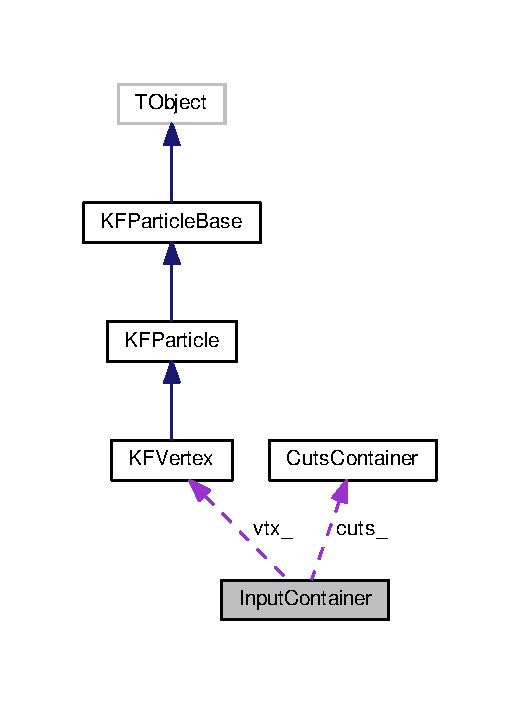
\includegraphics[width=250pt]{classInputContainer__coll__graph}
\end{center}
\end{figure}
\subsection*{Public Member Functions}
\begin{DoxyCompactItemize}
\item 
void {\bfseries Set\+PV} (float x, float y, float z)\hypertarget{classInputContainer_ad06aaffdb0b096eb2ed9c6cfa3250d42}{}\label{classInputContainer_ad06aaffdb0b096eb2ed9c6cfa3250d42}

\item 
void {\bfseries Set\+PV} (\hyperlink{classKFVertex}{K\+F\+Vertex} vertex)\hypertarget{classInputContainer_a40505cae1ae3a2217a59b772fa44a6df}{}\label{classInputContainer_a40505cae1ae3a2217a59b772fa44a6df}

\item 
void {\bfseries Set\+PV} (\hyperlink{classKFPVertex}{K\+F\+P\+Vertex} vertex)\hypertarget{classInputContainer_a7de3b46343227047f6dbd70e36e72ccf}{}\label{classInputContainer_a7de3b46343227047f6dbd70e36e72ccf}

\item 
void {\bfseries Add\+Track} (float x, float y, float z, float px, float py, float pz, std\+::vector$<$ float $>$ cov, float field\mbox{[}10\mbox{]}, int charge, int pdg, int id, int nhits=4, int passcuts=1)\hypertarget{classInputContainer_a53342c390b742ea13123c792007b8ca3}{}\label{classInputContainer_a53342c390b742ea13123c792007b8ca3}

\item 
\hyperlink{classKFParticleTopoReconstructor}{K\+F\+Particle\+Topo\+Reconstructor} $\ast$ {\bfseries Create\+Topo\+Reconstructor} ()\hypertarget{classInputContainer_aedadbb7d4f78e927027aa4acb7793f8f}{}\label{classInputContainer_aedadbb7d4f78e927027aa4acb7793f8f}

\item 
\hyperlink{classSimpleFinder}{Simple\+Finder} {\bfseries Create\+Simple\+Finder} ()\hypertarget{classInputContainer_a3aa4cca1fc8ec2cf0b124c78e01b6658}{}\label{classInputContainer_a3aa4cca1fc8ec2cf0b124c78e01b6658}

\item 
void {\bfseries Set\+Cuts} (const \hyperlink{classCutsContainer}{Cuts\+Container} \&cuts)\hypertarget{classInputContainer_a1f085ead392f5b6e79236514dfdba9b5}{}\label{classInputContainer_a1f085ead392f5b6e79236514dfdba9b5}

\end{DoxyCompactItemize}
\subsection*{Protected Member Functions}
\begin{DoxyCompactItemize}
\item 
double {\bfseries Inversed\+Chi2\+Prob} (double p, int ndf) const \hypertarget{classInputContainer_a73bcf36b0263f16c334b97661fae0eea}{}\label{classInputContainer_a73bcf36b0263f16c334b97661fae0eea}

\end{DoxyCompactItemize}
\subsection*{Protected Attributes}
\begin{DoxyCompactItemize}
\item 
\hyperlink{classKFVertex}{K\+F\+Vertex} {\bfseries vtx\+\_\+}\hypertarget{classInputContainer_a66b98870925df549191771baa3f7a789}{}\label{classInputContainer_a66b98870925df549191771baa3f7a789}

\item 
std\+::vector$<$ \hyperlink{classKFParticle}{K\+F\+Particle} $>$ {\bfseries tracks\+\_\+}\hypertarget{classInputContainer_a87ee73c56e8c5bf1d77483864881e473}{}\label{classInputContainer_a87ee73c56e8c5bf1d77483864881e473}

\item 
\hyperlink{classCutsContainer}{Cuts\+Container} {\bfseries cuts\+\_\+}\hypertarget{classInputContainer_af65fc096dd7c157dac46a3ed88432a64}{}\label{classInputContainer_af65fc096dd7c157dac46a3ed88432a64}

\end{DoxyCompactItemize}


\subsection{Detailed Description}
Container with input information about event (vertex and tracks) and cuts used in the certain event. 

\begin{DoxyAuthor}{Authors}
Oleksii Lubynets, Viktor Klochkov, Ilya Selyuzhenkov
\end{DoxyAuthor}
Each event is characterized with primary vertex, set of tracks and set of cuts (in general case cuts for different events can be different).~\newline
Primary vertex is characterized with its coordinates \{x, y, z\} and optionally with corresponding covariation matrix.~\newline
In order to store primary vertex the \hyperlink{classKFVertex}{K\+F\+Vertex} object is used. Each track is characterized with\+:~\newline
x, y, z -\/ three coordinates of point where it is defined;~\newline
px, py, pz -\/ three components of its momentum in this point;~\newline
cov -\/ covariation matrix of parameters mentioned above;~\newline
field\mbox{[}0\mbox{]} -\/ field\mbox{[}8\mbox{]} -\/ magnetic field approximation coefficients along the track\textquotesingle{}s trajectory field\mbox{[}9\mbox{]} -\/ reference point for MF coefficients;~\newline
charge -\/ its charge;~\newline
pdg -\/ P\+ID hypothesis for the track;~\newline
id -\/ its unique number (conserves through all the algorithm);~\newline
nhits -\/ number of hits in the tracking system which belong to the track. Is not used in the current version of K\+F\+P\+Simple, so default value 4 can be used;~\newline
passcuts -\/ flag variable which shows whether track satisfies pre-\/selection criteria. By default passcuts=1 should be used. ~\newline
In order to store tracks the vector of \hyperlink{classKFParticle}{K\+F\+Particle} objects is used.~\newline
In order to store cut values used for current event the \hyperlink{classCutsContainer}{Cuts\+Container} object is used. 

The documentation for this class was generated from the following files\+:\begin{DoxyCompactItemize}
\item 
/home/user/cbmdir/kfpf/\+K\+F\+Particle/\+Interface/Input\+Container.\+h\item 
/home/user/cbmdir/kfpf/\+K\+F\+Particle/\+Interface/Input\+Container.\+cxx\end{DoxyCompactItemize}

\hypertarget{classKFEfficiencyParticleInfo}{}\section{K\+F\+Efficiency\+Particle\+Info Class Reference}
\label{classKFEfficiencyParticleInfo}\index{K\+F\+Efficiency\+Particle\+Info@{K\+F\+Efficiency\+Particle\+Info}}


A helper class to define parameters of the decay list in \hyperlink{classKFPartEfficiencies}{K\+F\+Part\+Efficiencies}.  




{\ttfamily \#include $<$K\+F\+Part\+Efficiencies.\+h$>$}

\subsection*{Public Member Functions}
\begin{DoxyCompactItemize}
\item 
\hyperlink{classKFEfficiencyParticleInfo_a20377d0abc5f6bf03603ab1bf296f2ae}{K\+F\+Efficiency\+Particle\+Info} (std\+::string name, std\+::string title, int pdg, float histo\+Min, float histo\+Max, float mass, float life\+Time, int charge, float mass\+Sigma)\hypertarget{classKFEfficiencyParticleInfo_a20377d0abc5f6bf03603ab1bf296f2ae}{}\label{classKFEfficiencyParticleInfo_a20377d0abc5f6bf03603ab1bf296f2ae}

\begin{DoxyCompactList}\small\item\em Constructor with all parameters set in. There is no other way to define the parameters other then use this constructor. \end{DoxyCompactList}\item 
std\+::string \hyperlink{classKFEfficiencyParticleInfo_a517f4dc2cc4b876af682b05c5138e9bf}{Name} () const \hypertarget{classKFEfficiencyParticleInfo_a517f4dc2cc4b876af682b05c5138e9bf}{}\label{classKFEfficiencyParticleInfo_a517f4dc2cc4b876af682b05c5138e9bf}

\begin{DoxyCompactList}\small\item\em Returns name of the decay in the file with histograms. \end{DoxyCompactList}\item 
std\+::string \hyperlink{classKFEfficiencyParticleInfo_a4d5b802258b32925c890d9e8feb22b6f}{Title} () const \hypertarget{classKFEfficiencyParticleInfo_a4d5b802258b32925c890d9e8feb22b6f}{}\label{classKFEfficiencyParticleInfo_a4d5b802258b32925c890d9e8feb22b6f}

\begin{DoxyCompactList}\small\item\em Returns name of the decay in the output table with efficiency. \end{DoxyCompactList}\item 
int \hyperlink{classKFEfficiencyParticleInfo_aba5e25b80f6cd793d9234c4421e86904}{P\+DG} () const \hypertarget{classKFEfficiencyParticleInfo_aba5e25b80f6cd793d9234c4421e86904}{}\label{classKFEfficiencyParticleInfo_aba5e25b80f6cd793d9234c4421e86904}

\begin{DoxyCompactList}\small\item\em Returns the assigned P\+DG code. \end{DoxyCompactList}\item 
float \hyperlink{classKFEfficiencyParticleInfo_a76caa591241e85107d99366489fee56d}{Histo\+Min} () const \hypertarget{classKFEfficiencyParticleInfo_a76caa591241e85107d99366489fee56d}{}\label{classKFEfficiencyParticleInfo_a76caa591241e85107d99366489fee56d}

\begin{DoxyCompactList}\small\item\em Returns lower boundary in the mass histogram for the current decay. \end{DoxyCompactList}\item 
float \hyperlink{classKFEfficiencyParticleInfo_aee222cb7840e42c559ee4355b5eaf758}{Histo\+Max} () const \hypertarget{classKFEfficiencyParticleInfo_aee222cb7840e42c559ee4355b5eaf758}{}\label{classKFEfficiencyParticleInfo_aee222cb7840e42c559ee4355b5eaf758}

\begin{DoxyCompactList}\small\item\em Returns upper boundary in the mass histogram for the current decay. \end{DoxyCompactList}\item 
float \hyperlink{classKFEfficiencyParticleInfo_a89d8bf25bd33ac18f59e91c442c5b203}{Mass} () const \hypertarget{classKFEfficiencyParticleInfo_a89d8bf25bd33ac18f59e91c442c5b203}{}\label{classKFEfficiencyParticleInfo_a89d8bf25bd33ac18f59e91c442c5b203}

\begin{DoxyCompactList}\small\item\em Returns table mass of the particle. \end{DoxyCompactList}\item 
float \hyperlink{classKFEfficiencyParticleInfo_ae9876ae7a99238a95f626da9eb6c4b83}{Life\+Time} () const \hypertarget{classKFEfficiencyParticleInfo_ae9876ae7a99238a95f626da9eb6c4b83}{}\label{classKFEfficiencyParticleInfo_ae9876ae7a99238a95f626da9eb6c4b83}

\begin{DoxyCompactList}\small\item\em Returns lifetime of the particle. \end{DoxyCompactList}\item 
int \hyperlink{classKFEfficiencyParticleInfo_a9356a85bc4c1a0c13c906c909aa9d8af}{Charge} () const \hypertarget{classKFEfficiencyParticleInfo_a9356a85bc4c1a0c13c906c909aa9d8af}{}\label{classKFEfficiencyParticleInfo_a9356a85bc4c1a0c13c906c909aa9d8af}

\begin{DoxyCompactList}\small\item\em Returns charge of the particle in units of the elementary charge. \end{DoxyCompactList}\item 
float \hyperlink{classKFEfficiencyParticleInfo_af0c07beebc5c92c6836fae18f8df103b}{Mass\+Sigma} () const \hypertarget{classKFEfficiencyParticleInfo_af0c07beebc5c92c6836fae18f8df103b}{}\label{classKFEfficiencyParticleInfo_af0c07beebc5c92c6836fae18f8df103b}

\begin{DoxyCompactList}\small\item\em Returns expected width of the mass peak, used in the side bands method. \end{DoxyCompactList}\end{DoxyCompactItemize}


\subsection{Detailed Description}
A helper class to define parameters of the decay list in \hyperlink{classKFPartEfficiencies}{K\+F\+Part\+Efficiencies}. 

\begin{DoxyAuthor}{Author}
M.\+Zyzak, I.\+Kisel 
\end{DoxyAuthor}
\begin{DoxyDate}{Date}
05.\+02.\+2019 
\end{DoxyDate}
\begin{DoxyVersion}{Version}
1.\+0 
\end{DoxyVersion}


The documentation for this class was generated from the following file\+:\begin{DoxyCompactItemize}
\item 
/home/user/cbmdir/kfpf/\+K\+F\+Particle/\+K\+F\+Particle\+Performance/K\+F\+Part\+Efficiencies.\+h\end{DoxyCompactItemize}

\hypertarget{structKFMCCounter}{}\section{K\+F\+M\+C\+Counter$<$ T $>$ Class Template Reference}
\label{structKFMCCounter}\index{K\+F\+M\+C\+Counter$<$ T $>$@{K\+F\+M\+C\+Counter$<$ T $>$}}


A helper structure to store information on the number of reconstructed and Monte Carlo particles for efficiency calculation.  




{\ttfamily \#include $<$K\+F\+M\+C\+Counter.\+h$>$}

\subsection*{Public Member Functions}
\begin{DoxyCompactItemize}
\item 
\hyperlink{structKFMCCounter_a8a32841062b0acaf28a548738ea87c5d}{K\+F\+M\+C\+Counter} (int n\+Counters)\hypertarget{structKFMCCounter_a8a32841062b0acaf28a548738ea87c5d}{}\label{structKFMCCounter_a8a32841062b0acaf28a548738ea87c5d}

\begin{DoxyCompactList}\small\item\em Constructs the object with the set of counters \char`\"{}n\+Counters\char`\"{}. \end{DoxyCompactList}\item 
void \hyperlink{structKFMCCounter_a59d6f72b851528fd3c2288c9781a13aa}{Add\+Counter} ()\hypertarget{structKFMCCounter_a59d6f72b851528fd3c2288c9781a13aa}{}\label{structKFMCCounter_a59d6f72b851528fd3c2288c9781a13aa}

\begin{DoxyCompactList}\small\item\em Adds a counter to the existing list. \end{DoxyCompactList}\item 
void \hyperlink{structKFMCCounter_a659cea7b8ede07c088d1410bd043371c}{Add\+Counters} (int n\+Counters)\hypertarget{structKFMCCounter_a659cea7b8ede07c088d1410bd043371c}{}\label{structKFMCCounter_a659cea7b8ede07c088d1410bd043371c}

\begin{DoxyCompactList}\small\item\em Adds several counters to the existing list. \end{DoxyCompactList}\item 
\hyperlink{structKFMCCounter}{K\+F\+M\+C\+Counter} \& \hyperlink{structKFMCCounter_a757eb657a8f3ebda472b20a190643770}{operator+=} (\hyperlink{structKFMCCounter}{K\+F\+M\+C\+Counter} \&a)
\item 
\hyperlink{structKFMCCounter}{K\+F\+M\+C\+Counter} \hyperlink{structKFMCCounter_a94d9a8052083940bb40f04c7d8569210}{operator+} (\hyperlink{structKFMCCounter}{K\+F\+M\+C\+Counter} \&a)
\item 
{\footnotesize template$<$typename T2 $>$ }\\\hyperlink{structKFMCCounter}{K\+F\+M\+C\+Counter}$<$ double $>$ \hyperlink{structKFMCCounter_a1e0dabec8f1a0f51d4a45d20a250063f}{operator/} (\hyperlink{structKFMCCounter}{K\+F\+M\+C\+Counter}$<$ T2 $>$ \&a)
\item 
{\footnotesize template$<$typename T2 $>$ }\\\hyperlink{structKFMCCounter}{K\+F\+M\+C\+Counter}$<$ T2 $>$ \hyperlink{structKFMCCounter_a7f2f213ca3e091b7dc671b47625fe247}{operator/} (double a)
\end{DoxyCompactItemize}
\subsection*{Public Attributes}
\begin{DoxyCompactItemize}
\item 
int \hyperlink{structKFMCCounter_a5d2edf4a48889d68f9aa500ec6df4f18}{N\+Counters}\hypertarget{structKFMCCounter_a5d2edf4a48889d68f9aa500ec6df4f18}{}\label{structKFMCCounter_a5d2edf4a48889d68f9aa500ec6df4f18}

\begin{DoxyCompactList}\small\item\em Number of counters in the current object. \end{DoxyCompactList}\item 
std\+::vector$<$ T $>$ \hyperlink{structKFMCCounter_abbaf119d4b54cec95102245490f065ab}{counters}\hypertarget{structKFMCCounter_abbaf119d4b54cec95102245490f065ab}{}\label{structKFMCCounter_abbaf119d4b54cec95102245490f065ab}

\begin{DoxyCompactList}\small\item\em Counters of different set of particles. \end{DoxyCompactList}\end{DoxyCompactItemize}
\subsection*{Friends}
\begin{DoxyCompactItemize}
\item 
std\+::fstream \& \hyperlink{structKFMCCounter_a5c122439188dbe1105d9f394d4b0e259}{operator$<$$<$} (std\+::fstream \&strm, const \hyperlink{structKFMCCounter}{K\+F\+M\+C\+Counter}$<$ T $>$ \&a)
\item 
std\+::ostream \& \hyperlink{structKFMCCounter_a5346708c028a5cf1102259c5544c14f5}{operator$<$$<$} (std\+::ostream \&strm, const \hyperlink{structKFMCCounter}{K\+F\+M\+C\+Counter}$<$ T $>$ \&a)
\item 
std\+::fstream \& \hyperlink{structKFMCCounter_a8a4d328504a9f4340b557a8c15de4ef3}{operator$>$$>$} (std\+::fstream \&strm, \hyperlink{structKFMCCounter}{K\+F\+M\+C\+Counter}$<$ T $>$ \&a)
\end{DoxyCompactItemize}


\subsection{Detailed Description}
\subsubsection*{template$<$typename T$>$\\*
class K\+F\+M\+C\+Counter$<$ T $>$}

A helper structure to store information on the number of reconstructed and Monte Carlo particles for efficiency calculation. 

\begin{DoxyAuthor}{Author}
M.\+Zyzak, I.\+Kisel 
\end{DoxyAuthor}
\begin{DoxyDate}{Date}
05.\+02.\+2019 
\end{DoxyDate}
\begin{DoxyVersion}{Version}
1.\+0
\end{DoxyVersion}
The class is used to calculate reconstruction efficiency and ratios of a given set of particles. 

\subsection{Member Function Documentation}
\index{K\+F\+M\+C\+Counter@{K\+F\+M\+C\+Counter}!operator+@{operator+}}
\index{operator+@{operator+}!K\+F\+M\+C\+Counter@{K\+F\+M\+C\+Counter}}
\subsubsection[{\texorpdfstring{operator+(\+K\+F\+M\+C\+Counter \&a)}{operator+(KFMCCounter &a)}}]{\setlength{\rightskip}{0pt plus 5cm}template$<$typename T$>$ {\bf K\+F\+M\+C\+Counter} {\bf K\+F\+M\+C\+Counter}$<$ T $>$\+::operator+ (
\begin{DoxyParamCaption}
\item[{{\bf K\+F\+M\+C\+Counter}$<$ T $>$ \&}]{a}
\end{DoxyParamCaption}
)\hspace{0.3cm}{\ttfamily [inline]}}\hypertarget{structKFMCCounter_a94d9a8052083940bb40f04c7d8569210}{}\label{structKFMCCounter_a94d9a8052083940bb40f04c7d8569210}
Operator adds all counters from object \char`\"{}a\char`\"{} to the current object, result is stored to the temporary object. Returns the temporary object. \index{K\+F\+M\+C\+Counter@{K\+F\+M\+C\+Counter}!operator+=@{operator+=}}
\index{operator+=@{operator+=}!K\+F\+M\+C\+Counter@{K\+F\+M\+C\+Counter}}
\subsubsection[{\texorpdfstring{operator+=(\+K\+F\+M\+C\+Counter \&a)}{operator+=(KFMCCounter &a)}}]{\setlength{\rightskip}{0pt plus 5cm}template$<$typename T$>$ {\bf K\+F\+M\+C\+Counter}\& {\bf K\+F\+M\+C\+Counter}$<$ T $>$\+::operator+= (
\begin{DoxyParamCaption}
\item[{{\bf K\+F\+M\+C\+Counter}$<$ T $>$ \&}]{a}
\end{DoxyParamCaption}
)\hspace{0.3cm}{\ttfamily [inline]}}\hypertarget{structKFMCCounter_a757eb657a8f3ebda472b20a190643770}{}\label{structKFMCCounter_a757eb657a8f3ebda472b20a190643770}
Operator adds all counters from object \char`\"{}a\char`\"{} to the current object. Returns the current object. \index{K\+F\+M\+C\+Counter@{K\+F\+M\+C\+Counter}!operator/@{operator/}}
\index{operator/@{operator/}!K\+F\+M\+C\+Counter@{K\+F\+M\+C\+Counter}}
\subsubsection[{\texorpdfstring{operator/(\+K\+F\+M\+C\+Counter$<$ T2 $>$ \&a)}{operator/(KFMCCounter< T2 > &a)}}]{\setlength{\rightskip}{0pt plus 5cm}template$<$typename T$>$ template$<$typename T2 $>$ {\bf K\+F\+M\+C\+Counter}$<$double$>$ {\bf K\+F\+M\+C\+Counter}$<$ T $>$\+::operator/ (
\begin{DoxyParamCaption}
\item[{{\bf K\+F\+M\+C\+Counter}$<$ T2 $>$ \&}]{a}
\end{DoxyParamCaption}
)\hspace{0.3cm}{\ttfamily [inline]}}\hypertarget{structKFMCCounter_a1e0dabec8f1a0f51d4a45d20a250063f}{}\label{structKFMCCounter_a1e0dabec8f1a0f51d4a45d20a250063f}
Operator divides all counters from the current object to the counters from object \char`\"{}a\char`\"{}, result is stored to the temporary object. Returns the temporary object. \index{K\+F\+M\+C\+Counter@{K\+F\+M\+C\+Counter}!operator/@{operator/}}
\index{operator/@{operator/}!K\+F\+M\+C\+Counter@{K\+F\+M\+C\+Counter}}
\subsubsection[{\texorpdfstring{operator/(double a)}{operator/(double a)}}]{\setlength{\rightskip}{0pt plus 5cm}template$<$typename T$>$ template$<$typename T2 $>$ {\bf K\+F\+M\+C\+Counter}$<$T2$>$ {\bf K\+F\+M\+C\+Counter}$<$ T $>$\+::operator/ (
\begin{DoxyParamCaption}
\item[{double}]{a}
\end{DoxyParamCaption}
)\hspace{0.3cm}{\ttfamily [inline]}}\hypertarget{structKFMCCounter_a7f2f213ca3e091b7dc671b47625fe247}{}\label{structKFMCCounter_a7f2f213ca3e091b7dc671b47625fe247}
Operator divides all counters from the current object to the value \char`\"{}a\char`\"{}, result is stored to the temporary object. Returns the temporary object. 

\subsection{Friends And Related Function Documentation}
\index{K\+F\+M\+C\+Counter@{K\+F\+M\+C\+Counter}!operator$<$$<$@{operator$<$$<$}}
\index{operator$<$$<$@{operator$<$$<$}!K\+F\+M\+C\+Counter@{K\+F\+M\+C\+Counter}}
\subsubsection[{\texorpdfstring{operator$<$$<$}{operator<<}}]{\setlength{\rightskip}{0pt plus 5cm}template$<$typename T$>$ std\+::fstream\& operator$<$$<$ (
\begin{DoxyParamCaption}
\item[{std\+::fstream \&}]{strm, }
\item[{const {\bf K\+F\+M\+C\+Counter}$<$ T $>$ \&}]{a}
\end{DoxyParamCaption}
)\hspace{0.3cm}{\ttfamily [friend]}}\hypertarget{structKFMCCounter_a5c122439188dbe1105d9f394d4b0e259}{}\label{structKFMCCounter_a5c122439188dbe1105d9f394d4b0e259}
Operator to write the object \char`\"{}a\char`\"{} to the file \char`\"{}strm\char`\"{}. \index{K\+F\+M\+C\+Counter@{K\+F\+M\+C\+Counter}!operator$<$$<$@{operator$<$$<$}}
\index{operator$<$$<$@{operator$<$$<$}!K\+F\+M\+C\+Counter@{K\+F\+M\+C\+Counter}}
\subsubsection[{\texorpdfstring{operator$<$$<$}{operator<<}}]{\setlength{\rightskip}{0pt plus 5cm}template$<$typename T$>$ std\+::ostream\& operator$<$$<$ (
\begin{DoxyParamCaption}
\item[{std\+::ostream \&}]{strm, }
\item[{const {\bf K\+F\+M\+C\+Counter}$<$ T $>$ \&}]{a}
\end{DoxyParamCaption}
)\hspace{0.3cm}{\ttfamily [friend]}}\hypertarget{structKFMCCounter_a5346708c028a5cf1102259c5544c14f5}{}\label{structKFMCCounter_a5346708c028a5cf1102259c5544c14f5}
Operator to write the object \char`\"{}a\char`\"{} to the stream \char`\"{}strm\char`\"{}. \index{K\+F\+M\+C\+Counter@{K\+F\+M\+C\+Counter}!operator$>$$>$@{operator$>$$>$}}
\index{operator$>$$>$@{operator$>$$>$}!K\+F\+M\+C\+Counter@{K\+F\+M\+C\+Counter}}
\subsubsection[{\texorpdfstring{operator$>$$>$}{operator>>}}]{\setlength{\rightskip}{0pt plus 5cm}template$<$typename T$>$ std\+::fstream\& operator$>$$>$ (
\begin{DoxyParamCaption}
\item[{std\+::fstream \&}]{strm, }
\item[{{\bf K\+F\+M\+C\+Counter}$<$ T $>$ \&}]{a}
\end{DoxyParamCaption}
)\hspace{0.3cm}{\ttfamily [friend]}}\hypertarget{structKFMCCounter_a8a4d328504a9f4340b557a8c15de4ef3}{}\label{structKFMCCounter_a8a4d328504a9f4340b557a8c15de4ef3}
Operator to read the object \char`\"{}a\char`\"{} from the file \char`\"{}strm\char`\"{}. 

The documentation for this class was generated from the following file\+:\begin{DoxyCompactItemize}
\item 
/home/user/cbmdir/kfpf/\+K\+F\+Particle/\+K\+F\+Particle\+Performance/K\+F\+M\+C\+Counter.\+h\end{DoxyCompactItemize}

\hypertarget{classKFMCParticle}{}\section{K\+F\+M\+C\+Particle Class Reference}
\label{classKFMCParticle}\index{K\+F\+M\+C\+Particle@{K\+F\+M\+C\+Particle}}


A class to store relations between mother and daughter Monte Carlo simulated particles.  




{\ttfamily \#include $<$K\+F\+M\+C\+Particle.\+h$>$}



Inheritance diagram for K\+F\+M\+C\+Particle\+:
\nopagebreak
\begin{figure}[H]
\begin{center}
\leavevmode
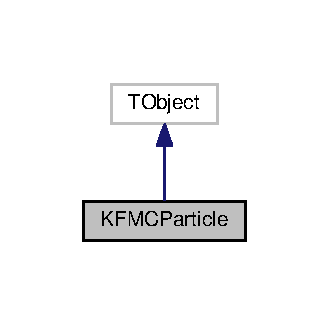
\includegraphics[width=158pt]{classKFMCParticle__inherit__graph}
\end{center}
\end{figure}


Collaboration diagram for K\+F\+M\+C\+Particle\+:
\nopagebreak
\begin{figure}[H]
\begin{center}
\leavevmode
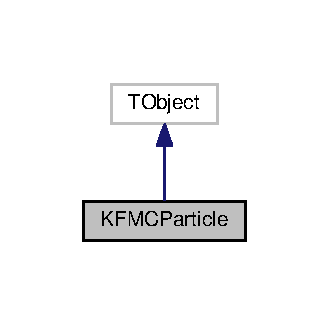
\includegraphics[width=158pt]{classKFMCParticle__coll__graph}
\end{center}
\end{figure}
\subsection*{Public Member Functions}
\begin{DoxyCompactItemize}
\item 
void \hyperlink{classKFMCParticle_afbccaab44cbd883748b589baf180bf8e}{Add\+Daughter} (int i)\hypertarget{classKFMCParticle_afbccaab44cbd883748b589baf180bf8e}{}\label{classKFMCParticle_afbccaab44cbd883748b589baf180bf8e}

\begin{DoxyCompactList}\small\item\em Adds an Id of the new particle to the list with Ids of daughter particles. \end{DoxyCompactList}\item 
int \hyperlink{classKFMCParticle_ae14cc6f58e668c7d3feb6bedbae57625}{N\+Daughters} () const \hypertarget{classKFMCParticle_ae14cc6f58e668c7d3feb6bedbae57625}{}\label{classKFMCParticle_ae14cc6f58e668c7d3feb6bedbae57625}

\begin{DoxyCompactList}\small\item\em Returns number of daughter particles. \end{DoxyCompactList}\item 
const std\+::vector$<$ int $>$ \& \hyperlink{classKFMCParticle_aa57d249e258adf12f022b58d8ad90d50}{Get\+Daughter\+Ids} () const \hypertarget{classKFMCParticle_aa57d249e258adf12f022b58d8ad90d50}{}\label{classKFMCParticle_aa57d249e258adf12f022b58d8ad90d50}

\begin{DoxyCompactList}\small\item\em Returns a reference to the vector with Id of daughter particle K\+F\+M\+C\+Particle\+::f\+Daughter\+Ids. \end{DoxyCompactList}\item 
void \hyperlink{classKFMCParticle_a57b4d9705f854d3a1717064aad0008fd}{Clean\+Daughters} ()\hypertarget{classKFMCParticle_a57b4d9705f854d3a1717064aad0008fd}{}\label{classKFMCParticle_a57b4d9705f854d3a1717064aad0008fd}

\begin{DoxyCompactList}\small\item\em Remove Ids of all daughter particles from the current object. \end{DoxyCompactList}\item 
void \hyperlink{classKFMCParticle_adb2ccad0b4b39acdf548b943b7a0ab91}{Set\+P\+DG} (int pdg)\hypertarget{classKFMCParticle_adb2ccad0b4b39acdf548b943b7a0ab91}{}\label{classKFMCParticle_adb2ccad0b4b39acdf548b943b7a0ab91}

\begin{DoxyCompactList}\small\item\em Set the P\+DG code of the current particle K\+F\+M\+C\+Particle\+::f\+P\+DG. \end{DoxyCompactList}\item 
void \hyperlink{classKFMCParticle_a4fe74ad782d04824601179c61085d82e}{Set\+M\+C\+Track\+ID} (int id)\hypertarget{classKFMCParticle_a4fe74ad782d04824601179c61085d82e}{}\label{classKFMCParticle_a4fe74ad782d04824601179c61085d82e}

\begin{DoxyCompactList}\small\item\em Sets the Id of the corresponding Monte Carlo track K\+F\+M\+C\+Particle\+::f\+M\+C\+Track\+ID. \end{DoxyCompactList}\item 
void \hyperlink{classKFMCParticle_aefeec3e0848ea6e94dfd48ba7dae077e}{Set\+Mother\+Id} (int id)\hypertarget{classKFMCParticle_aefeec3e0848ea6e94dfd48ba7dae077e}{}\label{classKFMCParticle_aefeec3e0848ea6e94dfd48ba7dae077e}

\begin{DoxyCompactList}\small\item\em Sets the Id of the mother particle or primary vertex K\+F\+M\+C\+Particle\+::f\+Mother\+Id. \end{DoxyCompactList}\item 
int \hyperlink{classKFMCParticle_adbf6a0b3aa66d2488e0dd35cd39e5307}{Get\+M\+C\+Track\+ID} () const \hypertarget{classKFMCParticle_adbf6a0b3aa66d2488e0dd35cd39e5307}{}\label{classKFMCParticle_adbf6a0b3aa66d2488e0dd35cd39e5307}

\begin{DoxyCompactList}\small\item\em Returns Id of the corresponding MC track K\+F\+M\+C\+Particle\+::f\+M\+C\+Track\+ID. \end{DoxyCompactList}\item 
int \hyperlink{classKFMCParticle_a1cd7e3ef51e4e2bb2ea3558feb5ab869}{Get\+Mother\+Id} () const \hypertarget{classKFMCParticle_a1cd7e3ef51e4e2bb2ea3558feb5ab869}{}\label{classKFMCParticle_a1cd7e3ef51e4e2bb2ea3558feb5ab869}

\begin{DoxyCompactList}\small\item\em Returns Id of the mother particle or primary vertex K\+F\+M\+C\+Particle\+::f\+Mother\+Id. \end{DoxyCompactList}\item 
int \hyperlink{classKFMCParticle_a9a26385ba40065086b9d6c0d0bbf4377}{Get\+P\+DG} () const \hypertarget{classKFMCParticle_a9a26385ba40065086b9d6c0d0bbf4377}{}\label{classKFMCParticle_a9a26385ba40065086b9d6c0d0bbf4377}

\begin{DoxyCompactList}\small\item\em Returns P\+DG code of the current particle K\+F\+M\+C\+Particle\+::f\+P\+DG. \end{DoxyCompactList}\item 
bool \hyperlink{classKFMCParticle_a6b354cb8e1e6e0cc1a93afd0be776838}{Is\+Reconstructable} (int i) const \hypertarget{classKFMCParticle_a6b354cb8e1e6e0cc1a93afd0be776838}{}\label{classKFMCParticle_a6b354cb8e1e6e0cc1a93afd0be776838}

\begin{DoxyCompactList}\small\item\em Returns a flag showing if particle can be reconstructed with K\+F\+M\+C\+Particle\+::f\+Is\+Reconstructable index \char`\"{}i\char`\"{}. \end{DoxyCompactList}\item 
void \hyperlink{classKFMCParticle_a144383bd4e948e2cf1d854ee500618a8}{Set\+As\+Reconstructable} (int i)\hypertarget{classKFMCParticle_a144383bd4e948e2cf1d854ee500618a8}{}\label{classKFMCParticle_a144383bd4e948e2cf1d854ee500618a8}

\begin{DoxyCompactList}\small\item\em Defines the particle as those which should be reconstructed for the efficiency set \char`\"{}i\char`\"{}. \end{DoxyCompactList}\item 
bool \hyperlink{classKFMCParticle_a4e2f37ec9add6707e73f43882c4d10ff}{Is\+Reconstructable\+V0} (int i) const \hypertarget{classKFMCParticle_a4e2f37ec9add6707e73f43882c4d10ff}{}\label{classKFMCParticle_a4e2f37ec9add6707e73f43882c4d10ff}

\begin{DoxyCompactList}\small\item\em Returns a flag showing if particle is a reconstructable V0. \end{DoxyCompactList}\item 
void \hyperlink{classKFMCParticle_a8e889b928a3f842141a6a78d267dcf79}{Set\+As\+Reconstructable\+V0} (int i)\hypertarget{classKFMCParticle_a8e889b928a3f842141a6a78d267dcf79}{}\label{classKFMCParticle_a8e889b928a3f842141a6a78d267dcf79}

\begin{DoxyCompactList}\small\item\em Defines the particle as V0 which should be reconstructed for the efficiency set \char`\"{}i\char`\"{}. \end{DoxyCompactList}\item 
void \hyperlink{classKFMCParticle_a6b6eb0cf8d1dda247509a3a2900268e7}{Set\+Initial\+Particle\+Id} (int i)\hypertarget{classKFMCParticle_a6b6eb0cf8d1dda247509a3a2900268e7}{}\label{classKFMCParticle_a6b6eb0cf8d1dda247509a3a2900268e7}

\begin{DoxyCompactList}\small\item\em Sets Id of the Monte Carlo particle, from which the current particle was copied. \end{DoxyCompactList}\item 
int \hyperlink{classKFMCParticle_af86d0b3cd56d0bef0aa9cbc651ee2e1a}{Initial\+Particle\+Id} () const \hypertarget{classKFMCParticle_af86d0b3cd56d0bef0aa9cbc651ee2e1a}{}\label{classKFMCParticle_af86d0b3cd56d0bef0aa9cbc651ee2e1a}

\begin{DoxyCompactList}\small\item\em Returns the Id of the Monte Carlo particle, from which the current particle was copied. \end{DoxyCompactList}\end{DoxyCompactItemize}


\subsection{Detailed Description}
A class to store relations between mother and daughter Monte Carlo simulated particles. 

\begin{DoxyAuthor}{Author}
M.\+Zyzak, I.\+Kisel 
\end{DoxyAuthor}
\begin{DoxyDate}{Date}
05.\+02.\+2019 
\end{DoxyDate}
\begin{DoxyVersion}{Version}
1.\+0
\end{DoxyVersion}
The class is used to calculate reconstruction efficiency of all Monte Carlo particles. It is simplifies the procedure for short-\/lived particles. Contains a vector with unique Ids of all MC daughters, a unique Id of the corresponding MC track, a unique Id of the MC mother particle, the P\+DG code of the MC particle, flags showing if particle can be reconstructed according to several different definitions, flags showing if particle creates a secondary vertex with two or more daughters, an index of the initial particle Id in case of the K-\/$>$mu+nu and pi-\/$>$ mu+nu decays, since G\+E\+A\+NT engines do not store neutrinos. 

The documentation for this class was generated from the following files\+:\begin{DoxyCompactItemize}
\item 
/home/user/cbmdir/kfpf/\+K\+F\+Particle/\+K\+F\+Particle\+Performance/K\+F\+M\+C\+Particle.\+h\item 
/home/user/cbmdir/kfpf/\+K\+F\+Particle/\+K\+F\+Particle\+Performance/K\+F\+M\+C\+Particle.\+cxx\end{DoxyCompactItemize}

\hypertarget{classKFMCTrack}{}\section{K\+F\+M\+C\+Track Class Reference}
\label{classKFMCTrack}\index{K\+F\+M\+C\+Track@{K\+F\+M\+C\+Track}}


A class for storage of the Monte Carlo simulated track in the cartesian parametrisation.  




{\ttfamily \#include $<$K\+F\+M\+C\+Track.\+h$>$}

\subsection*{Public Member Functions}
\begin{DoxyCompactItemize}
\item 
int \hyperlink{classKFMCTrack_aee4ee150d6a40cd3b6980c0911b5baca}{Mother\+Id} () const \hypertarget{classKFMCTrack_aee4ee150d6a40cd3b6980c0911b5baca}{}\label{classKFMCTrack_aee4ee150d6a40cd3b6980c0911b5baca}

\begin{DoxyCompactList}\small\item\em Returns a uniqueue Id of the mother track or primary vertex \hyperlink{classKFMCTrack_a9e683b839f23428f807de774af689467}{K\+F\+M\+C\+Track\+::f\+Mother\+Id}. \end{DoxyCompactList}\item 
int \hyperlink{classKFMCTrack_a7886d5c74b5c4009d9ee4953708e3a93}{P\+DG} () const \hypertarget{classKFMCTrack_a7886d5c74b5c4009d9ee4953708e3a93}{}\label{classKFMCTrack_a7886d5c74b5c4009d9ee4953708e3a93}

\begin{DoxyCompactList}\small\item\em Returns P\+DG code of the track \hyperlink{classKFMCTrack_ac219c1249ea3583df69eaff39bb2058d}{K\+F\+M\+C\+Track\+::f\+P\+DG}. \end{DoxyCompactList}\item 
float \hyperlink{classKFMCTrack_a70a5cee126b92b46be6de1adbe960f6b}{Par} (int i) const \hypertarget{classKFMCTrack_a70a5cee126b92b46be6de1adbe960f6b}{}\label{classKFMCTrack_a70a5cee126b92b46be6de1adbe960f6b}

\begin{DoxyCompactList}\small\item\em Returns value of the parameter \hyperlink{classKFMCTrack_ab36c74aaad27e04eb0ae56afd538ba77}{K\+F\+M\+C\+Track\+::f\+Par} with index \char`\"{}i\char`\"{}. \end{DoxyCompactList}\item 
float \hyperlink{classKFMCTrack_ad510b77d425c6e1eeeacfdebe9f66f0d}{X} () const \hypertarget{classKFMCTrack_ad510b77d425c6e1eeeacfdebe9f66f0d}{}\label{classKFMCTrack_ad510b77d425c6e1eeeacfdebe9f66f0d}

\begin{DoxyCompactList}\small\item\em Returns X coordinate of the track at the origin position. \end{DoxyCompactList}\item 
float \hyperlink{classKFMCTrack_aecd7bdeb558cbfdf06af5cb61e83c59d}{Y} () const \hypertarget{classKFMCTrack_aecd7bdeb558cbfdf06af5cb61e83c59d}{}\label{classKFMCTrack_aecd7bdeb558cbfdf06af5cb61e83c59d}

\begin{DoxyCompactList}\small\item\em Returns Y coordinate of the track at the origin position. \end{DoxyCompactList}\item 
float \hyperlink{classKFMCTrack_a12b43839eb12800b20a1e471c919abdc}{Z} () const \hypertarget{classKFMCTrack_a12b43839eb12800b20a1e471c919abdc}{}\label{classKFMCTrack_a12b43839eb12800b20a1e471c919abdc}

\begin{DoxyCompactList}\small\item\em Returns Y coordinate of the track at the origin position. \end{DoxyCompactList}\item 
float \hyperlink{classKFMCTrack_a41124c1a17d96c313dc359900ddad4d6}{L} () const \hypertarget{classKFMCTrack_a41124c1a17d96c313dc359900ddad4d6}{}\label{classKFMCTrack_a41124c1a17d96c313dc359900ddad4d6}

\begin{DoxyCompactList}\small\item\em Returns distance from the origin of the track to a point \{0,0,0\}. \end{DoxyCompactList}\item 
float \hyperlink{classKFMCTrack_a0d02638aa1cc226394734843767d133b}{Px} () const \hypertarget{classKFMCTrack_a0d02638aa1cc226394734843767d133b}{}\label{classKFMCTrack_a0d02638aa1cc226394734843767d133b}

\begin{DoxyCompactList}\small\item\em Returns Px momentum component of the track at the origin position. \end{DoxyCompactList}\item 
float \hyperlink{classKFMCTrack_aae9cf1f3bcb19684e181a2ce91907c22}{Py} () const \hypertarget{classKFMCTrack_aae9cf1f3bcb19684e181a2ce91907c22}{}\label{classKFMCTrack_aae9cf1f3bcb19684e181a2ce91907c22}

\begin{DoxyCompactList}\small\item\em Returns Py momentum component of the track at the origin position. \end{DoxyCompactList}\item 
float \hyperlink{classKFMCTrack_ae195a31af880d220f6b8eeb40505fb05}{Pz} () const \hypertarget{classKFMCTrack_ae195a31af880d220f6b8eeb40505fb05}{}\label{classKFMCTrack_ae195a31af880d220f6b8eeb40505fb05}

\begin{DoxyCompactList}\small\item\em Returns Pz momentum component of the track at the origin position. \end{DoxyCompactList}\item 
float \hyperlink{classKFMCTrack_afaaa77ea16e048da48a10ecb27235433}{P} () const \hypertarget{classKFMCTrack_afaaa77ea16e048da48a10ecb27235433}{}\label{classKFMCTrack_afaaa77ea16e048da48a10ecb27235433}

\begin{DoxyCompactList}\small\item\em Returns momentum of the track. \end{DoxyCompactList}\item 
float \hyperlink{classKFMCTrack_ac15a4fddd79e4e9ff9c33ac57837ac25}{Pt} () const \hypertarget{classKFMCTrack_ac15a4fddd79e4e9ff9c33ac57837ac25}{}\label{classKFMCTrack_ac15a4fddd79e4e9ff9c33ac57837ac25}

\begin{DoxyCompactList}\small\item\em Returns transverse momentum of the track. \end{DoxyCompactList}\item 
const float $\ast$ \hyperlink{classKFMCTrack_a99849b9fff54ffbd99c277643d0007cf}{Par} () const \hypertarget{classKFMCTrack_a99849b9fff54ffbd99c277643d0007cf}{}\label{classKFMCTrack_a99849b9fff54ffbd99c277643d0007cf}

\begin{DoxyCompactList}\small\item\em Returns a pointer to the array with track parameters \hyperlink{classKFMCTrack_ab36c74aaad27e04eb0ae56afd538ba77}{K\+F\+M\+C\+Track\+::f\+Par}. \end{DoxyCompactList}\item 
int \hyperlink{classKFMCTrack_af7db977361c2867dd0c0d15fd0a64623}{N\+M\+C\+Points} () const \hypertarget{classKFMCTrack_af7db977361c2867dd0c0d15fd0a64623}{}\label{classKFMCTrack_af7db977361c2867dd0c0d15fd0a64623}

\begin{DoxyCompactList}\small\item\em Returns number of MC points \hyperlink{classKFMCTrack_ac261323b51266d63d1bb6335e8428600}{K\+F\+M\+C\+Track\+::f\+N\+M\+C\+Points}. \end{DoxyCompactList}\item 
int \hyperlink{classKFMCTrack_a7ee66bc8a0c3db8f3adc6db3c28ae754}{N\+M\+C\+Pixel\+Points} () const \hypertarget{classKFMCTrack_a7ee66bc8a0c3db8f3adc6db3c28ae754}{}\label{classKFMCTrack_a7ee66bc8a0c3db8f3adc6db3c28ae754}

\begin{DoxyCompactList}\small\item\em Returns number of MC points at the precise detectors \hyperlink{classKFMCTrack_a7e91b033a3f0856258c0906ed5bcb293}{K\+F\+M\+C\+Track\+::f\+N\+M\+C\+Pixel\+Points}. \end{DoxyCompactList}\item 
bool \hyperlink{classKFMCTrack_a48f50e99c1ee75e0f800457528fe50aa}{Is\+Reconstructed} () const \hypertarget{classKFMCTrack_a48f50e99c1ee75e0f800457528fe50aa}{}\label{classKFMCTrack_a48f50e99c1ee75e0f800457528fe50aa}

\begin{DoxyCompactList}\small\item\em Returns a flag showing if track was found by the reconstruction procedure. \end{DoxyCompactList}\item 
bool \hyperlink{classKFMCTrack_a1269c7bd6cd60539a825e3b5a47e3d0f}{Is\+Out\+Of\+Detector} () const \hypertarget{classKFMCTrack_a1269c7bd6cd60539a825e3b5a47e3d0f}{}\label{classKFMCTrack_a1269c7bd6cd60539a825e3b5a47e3d0f}

\begin{DoxyCompactList}\small\item\em Returns a flag showing if track was out of acceptance. \end{DoxyCompactList}\item 
void \hyperlink{classKFMCTrack_adaf79bfed6d62b84dfcf47ccad7a3f44}{Set\+Par} (int i, float v)\hypertarget{classKFMCTrack_adaf79bfed6d62b84dfcf47ccad7a3f44}{}\label{classKFMCTrack_adaf79bfed6d62b84dfcf47ccad7a3f44}

\begin{DoxyCompactList}\small\item\em Sets a value \char`\"{}v\char`\"{} to the parameter with index \char`\"{}i\char`\"{}. \end{DoxyCompactList}\item 
void \hyperlink{classKFMCTrack_a6542e6870ea3135baf4276173af332a7}{SetX} (float v)\hypertarget{classKFMCTrack_a6542e6870ea3135baf4276173af332a7}{}\label{classKFMCTrack_a6542e6870ea3135baf4276173af332a7}

\begin{DoxyCompactList}\small\item\em Sets X coordinate at the origin position of the track. \end{DoxyCompactList}\item 
void \hyperlink{classKFMCTrack_a1eee8ab8b857e1df2f838e071f7eb2be}{SetY} (float v)\hypertarget{classKFMCTrack_a1eee8ab8b857e1df2f838e071f7eb2be}{}\label{classKFMCTrack_a1eee8ab8b857e1df2f838e071f7eb2be}

\begin{DoxyCompactList}\small\item\em Sets Y coordinate at the origin position of the track. \end{DoxyCompactList}\item 
void \hyperlink{classKFMCTrack_ac3764ac661f38b2794516a8343b382a9}{SetZ} (float v)\hypertarget{classKFMCTrack_ac3764ac661f38b2794516a8343b382a9}{}\label{classKFMCTrack_ac3764ac661f38b2794516a8343b382a9}

\begin{DoxyCompactList}\small\item\em Sets Z coordinate at the origin position of the track. \end{DoxyCompactList}\item 
void \hyperlink{classKFMCTrack_ae3de4de46304b5dd10fc0aaca485273e}{Set\+Px} (float v)\hypertarget{classKFMCTrack_ae3de4de46304b5dd10fc0aaca485273e}{}\label{classKFMCTrack_ae3de4de46304b5dd10fc0aaca485273e}

\begin{DoxyCompactList}\small\item\em Sets Px momentum component at the origin position of the track. \end{DoxyCompactList}\item 
void \hyperlink{classKFMCTrack_a5cc227a890fa1d9becec4c9efea5885e}{Set\+Py} (float v)\hypertarget{classKFMCTrack_a5cc227a890fa1d9becec4c9efea5885e}{}\label{classKFMCTrack_a5cc227a890fa1d9becec4c9efea5885e}

\begin{DoxyCompactList}\small\item\em Sets Py momentum component at the origin position of the track. \end{DoxyCompactList}\item 
void \hyperlink{classKFMCTrack_ae3f18e9869735ca8f6445a543e92de18}{Set\+Pz} (float v)\hypertarget{classKFMCTrack_ae3f18e9869735ca8f6445a543e92de18}{}\label{classKFMCTrack_ae3f18e9869735ca8f6445a543e92de18}

\begin{DoxyCompactList}\small\item\em Sets Pz momentum component at the origin position of the track. \end{DoxyCompactList}\item 
void \hyperlink{classKFMCTrack_a20cb8b3106cd0e56f279be9c67dccd1d}{Set\+QP} (float v)\hypertarget{classKFMCTrack_a20cb8b3106cd0e56f279be9c67dccd1d}{}\label{classKFMCTrack_a20cb8b3106cd0e56f279be9c67dccd1d}

\begin{DoxyCompactList}\small\item\em Sets q/P at the origin position of the track. \end{DoxyCompactList}\item 
void \hyperlink{classKFMCTrack_a7d13f8bcf32f217ef7cea49930827085}{Set\+Mother\+Id} (int v)\hypertarget{classKFMCTrack_a7d13f8bcf32f217ef7cea49930827085}{}\label{classKFMCTrack_a7d13f8bcf32f217ef7cea49930827085}

\begin{DoxyCompactList}\small\item\em Sets a unique id of the mother track if track is secondary or primary vertex with a negative sign if it is primary. \end{DoxyCompactList}\item 
void \hyperlink{classKFMCTrack_acfb63d1ba31c5ebf903095870041d306}{Set\+P\+DG} (int v)\hypertarget{classKFMCTrack_acfb63d1ba31c5ebf903095870041d306}{}\label{classKFMCTrack_acfb63d1ba31c5ebf903095870041d306}

\begin{DoxyCompactList}\small\item\em Sets P\+DG code of the current track. \end{DoxyCompactList}\item 
void \hyperlink{classKFMCTrack_a0a3e04f8e0564059d1c8f74ccffb6751}{Set\+N\+M\+C\+Points} (int v)\hypertarget{classKFMCTrack_a0a3e04f8e0564059d1c8f74ccffb6751}{}\label{classKFMCTrack_a0a3e04f8e0564059d1c8f74ccffb6751}

\begin{DoxyCompactList}\small\item\em Sets number of MC points produced at the detector planes. \end{DoxyCompactList}\item 
void \hyperlink{classKFMCTrack_a9ee38a914b6c713dc92b37e21f7512db}{Set\+N\+M\+C\+Pixel\+Points} (int v)\hypertarget{classKFMCTrack_a9ee38a914b6c713dc92b37e21f7512db}{}\label{classKFMCTrack_a9ee38a914b6c713dc92b37e21f7512db}

\begin{DoxyCompactList}\small\item\em Sets number of the MC points produced at the precise detectors. \end{DoxyCompactList}\item 
void \hyperlink{classKFMCTrack_aa27185332c1ad2a7093130499f3776ee}{Set\+Reconstructed} ()\hypertarget{classKFMCTrack_aa27185332c1ad2a7093130499f3776ee}{}\label{classKFMCTrack_aa27185332c1ad2a7093130499f3776ee}

\begin{DoxyCompactList}\small\item\em Defines the track as reconstructed. \end{DoxyCompactList}\item 
void \hyperlink{classKFMCTrack_a2b5f295bc2b44990ff1f924183bee9ee}{Set\+Not\+Reconstructed} ()\hypertarget{classKFMCTrack_a2b5f295bc2b44990ff1f924183bee9ee}{}\label{classKFMCTrack_a2b5f295bc2b44990ff1f924183bee9ee}

\begin{DoxyCompactList}\small\item\em Defines the track as not reconstructed. \end{DoxyCompactList}\item 
void \hyperlink{classKFMCTrack_a2b91b7ed5a5250890d5a92a6e7cf31b7}{Set\+Out\+Of\+Detector} ()\hypertarget{classKFMCTrack_a2b91b7ed5a5250890d5a92a6e7cf31b7}{}\label{classKFMCTrack_a2b91b7ed5a5250890d5a92a6e7cf31b7}

\begin{DoxyCompactList}\small\item\em Defines the track out of acceptance. \end{DoxyCompactList}\end{DoxyCompactItemize}
\subsection*{Protected Attributes}
\begin{DoxyCompactItemize}
\item 
int \hyperlink{classKFMCTrack_a9e683b839f23428f807de774af689467}{f\+Mother\+Id}\hypertarget{classKFMCTrack_a9e683b839f23428f807de774af689467}{}\label{classKFMCTrack_a9e683b839f23428f807de774af689467}

\begin{DoxyCompactList}\small\item\em Index of the mother track in tracks array. If track is produced at the primary vertex (PV) negative value with the PV Id is assigned. \end{DoxyCompactList}\item 
int \hyperlink{classKFMCTrack_ac219c1249ea3583df69eaff39bb2058d}{f\+P\+DG}\hypertarget{classKFMCTrack_ac219c1249ea3583df69eaff39bb2058d}{}\label{classKFMCTrack_ac219c1249ea3583df69eaff39bb2058d}

\begin{DoxyCompactList}\small\item\em The P\+DG code of the current Monte Carlo track. \end{DoxyCompactList}\item 
float \hyperlink{classKFMCTrack_ab36c74aaad27e04eb0ae56afd538ba77}{f\+Par} \mbox{[}7\mbox{]}\hypertarget{classKFMCTrack_ab36c74aaad27e04eb0ae56afd538ba77}{}\label{classKFMCTrack_ab36c74aaad27e04eb0ae56afd538ba77}

\begin{DoxyCompactList}\small\item\em Parameters of the track\+: \{ X, Y, Z, Px, Py, Pz, q/P \}, where \char`\"{}q\char`\"{} is its charge. \end{DoxyCompactList}\item 
int \hyperlink{classKFMCTrack_ac261323b51266d63d1bb6335e8428600}{f\+N\+M\+C\+Points}\hypertarget{classKFMCTrack_ac261323b51266d63d1bb6335e8428600}{}\label{classKFMCTrack_ac261323b51266d63d1bb6335e8428600}

\begin{DoxyCompactList}\small\item\em Total number of Monte Carlo points produced by the simulation engine at the detector stations. \end{DoxyCompactList}\item 
int \hyperlink{classKFMCTrack_a7e91b033a3f0856258c0906ed5bcb293}{f\+N\+M\+C\+Pixel\+Points}\hypertarget{classKFMCTrack_a7e91b033a3f0856258c0906ed5bcb293}{}\label{classKFMCTrack_a7e91b033a3f0856258c0906ed5bcb293}

\begin{DoxyCompactList}\small\item\em Number of Monte Carlo points produced at the precise detectors (like M\+VD in C\+BM, H\+FT in S\+T\+AR, I\+TS in A\+L\+I\+CE, etc.). \end{DoxyCompactList}\item 
bool \hyperlink{classKFMCTrack_a7cfb459a6c51ee52e610d2405056eb9f}{f\+Is\+Reconstructed}\hypertarget{classKFMCTrack_a7cfb459a6c51ee52e610d2405056eb9f}{}\label{classKFMCTrack_a7cfb459a6c51ee52e610d2405056eb9f}

\begin{DoxyCompactList}\small\item\em A flag showing if track was found by the reconstruction procedure. Is required for correct efficiency calculation. \end{DoxyCompactList}\item 
bool \hyperlink{classKFMCTrack_a6375b38e77037425fb1499299c286fc4}{f\+Is\+Out\+Of\+Detector}\hypertarget{classKFMCTrack_a6375b38e77037425fb1499299c286fc4}{}\label{classKFMCTrack_a6375b38e77037425fb1499299c286fc4}

\begin{DoxyCompactList}\small\item\em A flag showing if track was out of acceptance. Is required for correct calculation of the acceptance. \end{DoxyCompactList}\end{DoxyCompactItemize}


\subsection{Detailed Description}
A class for storage of the Monte Carlo simulated track in the cartesian parametrisation. 

\begin{DoxyAuthor}{Author}
M.\+Zyzak, I.\+Kisel 
\end{DoxyAuthor}
\begin{DoxyDate}{Date}
05.\+02.\+2019 
\end{DoxyDate}
\begin{DoxyVersion}{Version}
1.\+0
\end{DoxyVersion}
A track is described with the parameters \{ X, Y, Z, Px, Py, Pz, q/P \}. Parameters are stored at the origin position. Class also contains Id of the mother track, P\+DG code for the current track, number of Monte Carlo points produced by the simulation engine at the detector stations, number of Monte Carlo points produced at the precise detectors (like M\+VD in C\+BM, H\+FT in S\+T\+AR, I\+TS in A\+L\+I\+CE, etc.). It also has a flag showing if track was found by the reconstruction procedure for efficiency calculation, and a flag showing if track was out of acceptance. 

The documentation for this class was generated from the following file\+:\begin{DoxyCompactItemize}
\item 
/home/user/cbmdir/kfpf/\+K\+F\+Particle/\+K\+F\+Particle\+Performance/K\+F\+M\+C\+Track.\+h\end{DoxyCompactItemize}

\hypertarget{classKFMCVertex}{}\section{K\+F\+M\+C\+Vertex Class Reference}
\label{classKFMCVertex}\index{K\+F\+M\+C\+Vertex@{K\+F\+M\+C\+Vertex}}


A class to store information about simulated Monte Carlo primary vertices.  




{\ttfamily \#include $<$K\+F\+M\+C\+Vertex.\+h$>$}

\subsection*{Public Member Functions}
\begin{DoxyCompactItemize}
\item 
float \hyperlink{classKFMCVertex_a3081f0e8c418770c5ea288a204638af3}{Par} (int i) const \hypertarget{classKFMCVertex_a3081f0e8c418770c5ea288a204638af3}{}\label{classKFMCVertex_a3081f0e8c418770c5ea288a204638af3}

\begin{DoxyCompactList}\small\item\em Returns parameter with index \char`\"{}i\char`\"{} from \hyperlink{classKFMCVertex_a647ebd7994aa422d5455a3f66d9bbff9}{K\+F\+M\+C\+Vertex\+::f\+Par}. \end{DoxyCompactList}\item 
float \hyperlink{classKFMCVertex_afd80435d29bb37bcbb5a9de88d1a89e4}{X} () const \hypertarget{classKFMCVertex_afd80435d29bb37bcbb5a9de88d1a89e4}{}\label{classKFMCVertex_afd80435d29bb37bcbb5a9de88d1a89e4}

\begin{DoxyCompactList}\small\item\em Returns X coordinate of the vertex. \end{DoxyCompactList}\item 
float \hyperlink{classKFMCVertex_abf64836dc4f3b0e88c95e5767c908c17}{Y} () const \hypertarget{classKFMCVertex_abf64836dc4f3b0e88c95e5767c908c17}{}\label{classKFMCVertex_abf64836dc4f3b0e88c95e5767c908c17}

\begin{DoxyCompactList}\small\item\em Returns Y coordinate of the vertex. \end{DoxyCompactList}\item 
float \hyperlink{classKFMCVertex_a4f4608d79cd24afa303f8bc952e02748}{Z} () const \hypertarget{classKFMCVertex_a4f4608d79cd24afa303f8bc952e02748}{}\label{classKFMCVertex_a4f4608d79cd24afa303f8bc952e02748}

\begin{DoxyCompactList}\small\item\em Returns Z coordinate of the vertex. \end{DoxyCompactList}\item 
const float $\ast$ \hyperlink{classKFMCVertex_ad2c78d7fd510edd7fc1f324442c9113c}{Get\+Par} () const \hypertarget{classKFMCVertex_ad2c78d7fd510edd7fc1f324442c9113c}{}\label{classKFMCVertex_ad2c78d7fd510edd7fc1f324442c9113c}

\begin{DoxyCompactList}\small\item\em Returns pointer to the parameters of the vertex \hyperlink{classKFMCVertex_a647ebd7994aa422d5455a3f66d9bbff9}{K\+F\+M\+C\+Vertex\+::f\+Par}. \end{DoxyCompactList}\item 
void \hyperlink{classKFMCVertex_a1e0ca1d5921cfdfcb071beae4b0492e4}{Set\+Par} (int i, float v)\hypertarget{classKFMCVertex_a1e0ca1d5921cfdfcb071beae4b0492e4}{}\label{classKFMCVertex_a1e0ca1d5921cfdfcb071beae4b0492e4}

\begin{DoxyCompactList}\small\item\em Sets a value \char`\"{}v\char`\"{} to parameter \char`\"{}i\char`\"{}. \end{DoxyCompactList}\item 
void \hyperlink{classKFMCVertex_a99b92b21117ac6047417327aaad2416a}{SetX} (float v)\hypertarget{classKFMCVertex_a99b92b21117ac6047417327aaad2416a}{}\label{classKFMCVertex_a99b92b21117ac6047417327aaad2416a}

\begin{DoxyCompactList}\small\item\em Sets value \char`\"{}v\char`\"{} to the X coordinate. \end{DoxyCompactList}\item 
void \hyperlink{classKFMCVertex_ae7eee5e4a16ca88f8da3fab3b307142b}{SetY} (float v)\hypertarget{classKFMCVertex_ae7eee5e4a16ca88f8da3fab3b307142b}{}\label{classKFMCVertex_ae7eee5e4a16ca88f8da3fab3b307142b}

\begin{DoxyCompactList}\small\item\em Sets value \char`\"{}v\char`\"{} to the Y coordinate. \end{DoxyCompactList}\item 
void \hyperlink{classKFMCVertex_a93f5b783902d6a8d244c06ddcc189967}{SetZ} (float v)\hypertarget{classKFMCVertex_a93f5b783902d6a8d244c06ddcc189967}{}\label{classKFMCVertex_a93f5b783902d6a8d244c06ddcc189967}

\begin{DoxyCompactList}\small\item\em Sets value \char`\"{}v\char`\"{} to the Z coordinate. \end{DoxyCompactList}\item 
int \hyperlink{classKFMCVertex_a51f3aafb24777a594684b2222769c8ee}{N\+Daughter\+Tracks} () const \hypertarget{classKFMCVertex_a51f3aafb24777a594684b2222769c8ee}{}\label{classKFMCVertex_a51f3aafb24777a594684b2222769c8ee}

\begin{DoxyCompactList}\small\item\em Returns number of Monte Carlo tracks produced at the current vertex. \end{DoxyCompactList}\item 
int \hyperlink{classKFMCVertex_a9e34c5cc68180b40c0a9c59e2408fd7e}{N\+Reconstructed\+Daughter\+Tracks} () const \hypertarget{classKFMCVertex_a9e34c5cc68180b40c0a9c59e2408fd7e}{}\label{classKFMCVertex_a9e34c5cc68180b40c0a9c59e2408fd7e}

\begin{DoxyCompactList}\small\item\em Returns number of reconstructed tracks from this vertex. \end{DoxyCompactList}\item 
void \hyperlink{classKFMCVertex_af2ccf2a07c048d97a40539482275e12a}{Add\+Daughter\+Track} (int i\+Tr)\hypertarget{classKFMCVertex_af2ccf2a07c048d97a40539482275e12a}{}\label{classKFMCVertex_af2ccf2a07c048d97a40539482275e12a}

\begin{DoxyCompactList}\small\item\em Adds unique id of the Monte Carlo track produced at the current vertex. \end{DoxyCompactList}\item 
int \hyperlink{classKFMCVertex_a8952b674a23b479a1ed642dcf8db3856}{Daughter\+Track} (int i\+Tr) const 
\item 
bool \hyperlink{classKFMCVertex_a87f06d29c10c29e62e62faea55cebdf9}{Is\+M\+C\+Reconstructable} () const \hypertarget{classKFMCVertex_a87f06d29c10c29e62e62faea55cebdf9}{}\label{classKFMCVertex_a87f06d29c10c29e62e62faea55cebdf9}

\begin{DoxyCompactList}\small\item\em Returns flag showing if the vertex can be found (definition is based on the MC tracks) \end{DoxyCompactList}\item 
bool \hyperlink{classKFMCVertex_a41a15930645f6801706e46d5c5c92497}{Is\+Reconstructable} () const \hypertarget{classKFMCVertex_a41a15930645f6801706e46d5c5c92497}{}\label{classKFMCVertex_a41a15930645f6801706e46d5c5c92497}

\begin{DoxyCompactList}\small\item\em Returns flag showing if the vertex can be found (definition is based on the reconstructed tracks) \end{DoxyCompactList}\item 
bool \hyperlink{classKFMCVertex_a46ac54d0520553cccee1e7f7217fe3fd}{Is\+Reconstructed} () const \hypertarget{classKFMCVertex_a46ac54d0520553cccee1e7f7217fe3fd}{}\label{classKFMCVertex_a46ac54d0520553cccee1e7f7217fe3fd}

\begin{DoxyCompactList}\small\item\em Returns flag showing if the vertex was reconstructed. \end{DoxyCompactList}\item 
void \hyperlink{classKFMCVertex_a116a277479a9eb7523202023d6bbd6ba}{Set\+Reconstructable} ()\hypertarget{classKFMCVertex_a116a277479a9eb7523202023d6bbd6ba}{}\label{classKFMCVertex_a116a277479a9eb7523202023d6bbd6ba}

\begin{DoxyCompactList}\small\item\em Defines the current vertex as such that can be reconstructed (based on the reconstructed tracks) \end{DoxyCompactList}\item 
void \hyperlink{classKFMCVertex_a0c8c2b357bbb7c690cfeb22fc025e795}{Set\+Un\+Reconstructable} ()\hypertarget{classKFMCVertex_a0c8c2b357bbb7c690cfeb22fc025e795}{}\label{classKFMCVertex_a0c8c2b357bbb7c690cfeb22fc025e795}

\begin{DoxyCompactList}\small\item\em Defines the current vertex as such that can not be reconstructed (based on the reconstructed tracks) \end{DoxyCompactList}\item 
void \hyperlink{classKFMCVertex_a2b334e879e9b429c7acebd727ac99ee1}{Set\+M\+C\+Reconstructable} ()\hypertarget{classKFMCVertex_a2b334e879e9b429c7acebd727ac99ee1}{}\label{classKFMCVertex_a2b334e879e9b429c7acebd727ac99ee1}

\begin{DoxyCompactList}\small\item\em Defines the current vertex as such that can be reconstructed (based on the MC tracks) \end{DoxyCompactList}\item 
void \hyperlink{classKFMCVertex_ac6fdfcc77e19dd3cc75de49b01843574}{Set\+M\+C\+Un\+Reconstructable} ()\hypertarget{classKFMCVertex_ac6fdfcc77e19dd3cc75de49b01843574}{}\label{classKFMCVertex_ac6fdfcc77e19dd3cc75de49b01843574}

\begin{DoxyCompactList}\small\item\em Defines the current vertex as such that can not be reconstructed (based on the MC tracks) \end{DoxyCompactList}\item 
void \hyperlink{classKFMCVertex_a3c20061e84e4df81331f095f64813fcf}{Set\+Reconstructed} ()\hypertarget{classKFMCVertex_a3c20061e84e4df81331f095f64813fcf}{}\label{classKFMCVertex_a3c20061e84e4df81331f095f64813fcf}

\begin{DoxyCompactList}\small\item\em Defines the current vertex as such that was reconstructed. \end{DoxyCompactList}\item 
void \hyperlink{classKFMCVertex_ae6338729915e9c39ef56bba7ba86af35}{Set\+Un\+Reconstructed} ()\hypertarget{classKFMCVertex_ae6338729915e9c39ef56bba7ba86af35}{}\label{classKFMCVertex_ae6338729915e9c39ef56bba7ba86af35}

\begin{DoxyCompactList}\small\item\em Defines the current vertex as such that was not reconstructed. \end{DoxyCompactList}\item 
void \hyperlink{classKFMCVertex_a801d833c5009f7bad8c136b68434c10a}{Set\+N\+Reconstructed\+Daughters} (int n)\hypertarget{classKFMCVertex_a801d833c5009f7bad8c136b68434c10a}{}\label{classKFMCVertex_a801d833c5009f7bad8c136b68434c10a}

\begin{DoxyCompactList}\small\item\em Defines number of the reconstructed tracks produced at the current vertex. \end{DoxyCompactList}\item 
bool \hyperlink{classKFMCVertex_a6858848001a3bffdf36e9c0644dfdf61}{Is\+Trigger\+PV} () const \hypertarget{classKFMCVertex_a6858848001a3bffdf36e9c0644dfdf61}{}\label{classKFMCVertex_a6858848001a3bffdf36e9c0644dfdf61}

\begin{DoxyCompactList}\small\item\em Returns flag showing if the vertex is considerred as tigger. \end{DoxyCompactList}\item 
void \hyperlink{classKFMCVertex_ac12fdb952def60c6233f34ca8ef75b6b}{Set\+Trigger\+PV} ()\hypertarget{classKFMCVertex_ac12fdb952def60c6233f34ca8ef75b6b}{}\label{classKFMCVertex_ac12fdb952def60c6233f34ca8ef75b6b}

\begin{DoxyCompactList}\small\item\em Defines the current vertex as the trigger primary vertex. \end{DoxyCompactList}\end{DoxyCompactItemize}
\subsection*{Protected Attributes}
\begin{DoxyCompactItemize}
\item 
float \hyperlink{classKFMCVertex_a647ebd7994aa422d5455a3f66d9bbff9}{f\+Par} \mbox{[}3\mbox{]}\hypertarget{classKFMCVertex_a647ebd7994aa422d5455a3f66d9bbff9}{}\label{classKFMCVertex_a647ebd7994aa422d5455a3f66d9bbff9}

\begin{DoxyCompactList}\small\item\em Cartesian coordinates of the vertex\+: \{ X, Y, Z \}. \end{DoxyCompactList}\item 
std\+::vector$<$ int $>$ \hyperlink{classKFMCVertex_a531546b4d9daed2c31383e90ad47a42b}{f\+Daughter\+Tracks}\hypertarget{classKFMCVertex_a531546b4d9daed2c31383e90ad47a42b}{}\label{classKFMCVertex_a531546b4d9daed2c31383e90ad47a42b}

\begin{DoxyCompactList}\small\item\em Vector with unique ids of the Monte Carlo tracks produced at this vertex. \end{DoxyCompactList}\item 
bool \hyperlink{classKFMCVertex_a47a4c3b574ca9b0a74e4613ecf326bb6}{f\+Is\+Reconstructable}\hypertarget{classKFMCVertex_a47a4c3b574ca9b0a74e4613ecf326bb6}{}\label{classKFMCVertex_a47a4c3b574ca9b0a74e4613ecf326bb6}

\begin{DoxyCompactList}\small\item\em Flag showing if the vertex considered as reconstructable based on the reconstructed tracks. \end{DoxyCompactList}\item 
bool \hyperlink{classKFMCVertex_a70ebe127df16f9f55051759292dabf52}{f\+Is\+M\+C\+Reconstructable}\hypertarget{classKFMCVertex_a70ebe127df16f9f55051759292dabf52}{}\label{classKFMCVertex_a70ebe127df16f9f55051759292dabf52}

\begin{DoxyCompactList}\small\item\em Flag showing if the vertex considered as reconstructable based on the Monte Carlo tracks. \end{DoxyCompactList}\item 
bool \hyperlink{classKFMCVertex_a1a064ccde676f3baa5f100f911dabe27}{f\+Is\+Reconstructed}\hypertarget{classKFMCVertex_a1a064ccde676f3baa5f100f911dabe27}{}\label{classKFMCVertex_a1a064ccde676f3baa5f100f911dabe27}

\begin{DoxyCompactList}\small\item\em Flag showing if vertex was reconstructed. \end{DoxyCompactList}\item 
int \hyperlink{classKFMCVertex_add1221f3483673f4641934d4933f5cd4}{f\+N\+Reconstructed\+Daughters}\hypertarget{classKFMCVertex_add1221f3483673f4641934d4933f5cd4}{}\label{classKFMCVertex_add1221f3483673f4641934d4933f5cd4}

\begin{DoxyCompactList}\small\item\em Number of found tracks, produced at the current vertex. \end{DoxyCompactList}\item 
bool \hyperlink{classKFMCVertex_a9e37d86942db0797e198ef4e61ab1867}{f\+Is\+Trigger\+PV}\hypertarget{classKFMCVertex_a9e37d86942db0797e198ef4e61ab1867}{}\label{classKFMCVertex_a9e37d86942db0797e198ef4e61ab1867}

\begin{DoxyCompactList}\small\item\em Flag showing if the vertex was a trigger primary vertex. \end{DoxyCompactList}\end{DoxyCompactItemize}
\subsection*{Friends}
\begin{DoxyCompactItemize}
\item 
std\+::ostream \& \hyperlink{classKFMCVertex_af066fb42a2f04f8027e74113d5940dae}{operator$<$$<$} (std\+::ostream \&out, const \hyperlink{classKFMCVertex}{K\+F\+M\+C\+Vertex} \&a)
\item 
std\+::istream \& \hyperlink{classKFMCVertex_a07f15138b33749b902ae133f7ec69cb0}{operator$>$$>$} (std\+::istream \&in, \hyperlink{classKFMCVertex}{K\+F\+M\+C\+Vertex} \&a)
\end{DoxyCompactItemize}


\subsection{Detailed Description}
A class to store information about simulated Monte Carlo primary vertices. 

\begin{DoxyAuthor}{Author}
M.\+Zyzak, I.\+Kisel 
\end{DoxyAuthor}
\begin{DoxyDate}{Date}
05.\+02.\+2019 
\end{DoxyDate}
\begin{DoxyVersion}{Version}
1.\+0
\end{DoxyVersion}
The class contains coordinates of the vertex, indices of the Monte Carlo tracks produced at this vertex, classification flags, number of the reconstructed Monte Carlo tracks. 

\subsection{Member Function Documentation}
\index{K\+F\+M\+C\+Vertex@{K\+F\+M\+C\+Vertex}!Daughter\+Track@{Daughter\+Track}}
\index{Daughter\+Track@{Daughter\+Track}!K\+F\+M\+C\+Vertex@{K\+F\+M\+C\+Vertex}}
\subsubsection[{\texorpdfstring{Daughter\+Track(int i\+Tr) const }{DaughterTrack(int iTr) const }}]{\setlength{\rightskip}{0pt plus 5cm}int K\+F\+M\+C\+Vertex\+::\+Daughter\+Track (
\begin{DoxyParamCaption}
\item[{int}]{i\+Tr}
\end{DoxyParamCaption}
) const\hspace{0.3cm}{\ttfamily [inline]}}\hypertarget{classKFMCVertex_a8952b674a23b479a1ed642dcf8db3856}{}\label{classKFMCVertex_a8952b674a23b479a1ed642dcf8db3856}
Returns unique id of the Monte Carlo track from this vertex with index \char`\"{}i\+Tr\char`\"{}. 
\begin{DoxyParams}[1]{Parameters}
\mbox{\tt in}  & {\em i\+Tr} & -\/ index of the track.\\
\hline
\end{DoxyParams}


\subsection{Friends And Related Function Documentation}
\index{K\+F\+M\+C\+Vertex@{K\+F\+M\+C\+Vertex}!operator$<$$<$@{operator$<$$<$}}
\index{operator$<$$<$@{operator$<$$<$}!K\+F\+M\+C\+Vertex@{K\+F\+M\+C\+Vertex}}
\subsubsection[{\texorpdfstring{operator$<$$<$}{operator<<}}]{\setlength{\rightskip}{0pt plus 5cm}std\+::ostream\& operator$<$$<$ (
\begin{DoxyParamCaption}
\item[{std\+::ostream \&}]{out, }
\item[{const {\bf K\+F\+M\+C\+Vertex} \&}]{a}
\end{DoxyParamCaption}
)\hspace{0.3cm}{\ttfamily [friend]}}\hypertarget{classKFMCVertex_af066fb42a2f04f8027e74113d5940dae}{}\label{classKFMCVertex_af066fb42a2f04f8027e74113d5940dae}
Operator to print coordinates of the MC vertex \char`\"{}a\char`\"{}. 
\begin{DoxyParams}[1]{Parameters}
\mbox{\tt in}  & {\em out} & -\/ stream, where coordinates will be printed \\
\hline
\mbox{\tt in}  & {\em a} & -\/ vertex to be printed\\
\hline
\end{DoxyParams}
\index{K\+F\+M\+C\+Vertex@{K\+F\+M\+C\+Vertex}!operator$>$$>$@{operator$>$$>$}}
\index{operator$>$$>$@{operator$>$$>$}!K\+F\+M\+C\+Vertex@{K\+F\+M\+C\+Vertex}}
\subsubsection[{\texorpdfstring{operator$>$$>$}{operator>>}}]{\setlength{\rightskip}{0pt plus 5cm}std\+::istream\& operator$>$$>$ (
\begin{DoxyParamCaption}
\item[{std\+::istream \&}]{in, }
\item[{{\bf K\+F\+M\+C\+Vertex} \&}]{a}
\end{DoxyParamCaption}
)\hspace{0.3cm}{\ttfamily [friend]}}\hypertarget{classKFMCVertex_a07f15138b33749b902ae133f7ec69cb0}{}\label{classKFMCVertex_a07f15138b33749b902ae133f7ec69cb0}
Operator to read coordinates of the vertex from the input stream. 
\begin{DoxyParams}[1]{Parameters}
\mbox{\tt in}  & {\em in} & -\/ input stream \\
\hline
\mbox{\tt in}  & {\em a} & -\/ vertex, where the coordinates will be read in\\
\hline
\end{DoxyParams}


The documentation for this class was generated from the following files\+:\begin{DoxyCompactItemize}
\item 
/home/user/cbmdir/kfpf/\+K\+F\+Particle/\+K\+F\+Particle\+Performance/K\+F\+M\+C\+Vertex.\+h\item 
/home/user/cbmdir/kfpf/\+K\+F\+Particle/\+K\+F\+Particle\+Performance/K\+F\+M\+C\+Vertex.\+cxx\end{DoxyCompactItemize}

\hypertarget{classKFPartEfficiencies}{}\section{K\+F\+Part\+Efficiencies Class Reference}
\label{classKFPartEfficiencies}\index{K\+F\+Part\+Efficiencies@{K\+F\+Part\+Efficiencies}}


Class to calculate efficiency of KF Particle Finder.  




{\ttfamily \#include $<$K\+F\+Part\+Efficiencies.\+h$>$}



Inheritance diagram for K\+F\+Part\+Efficiencies\+:\nopagebreak
\begin{figure}[H]
\begin{center}
\leavevmode
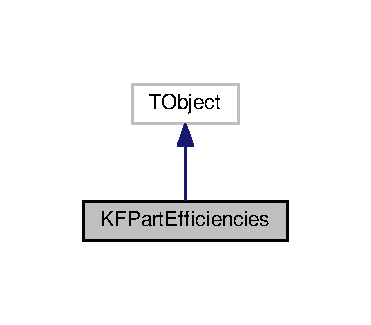
\includegraphics[width=178pt]{classKFPartEfficiencies__inherit__graph}
\end{center}
\end{figure}


Collaboration diagram for K\+F\+Part\+Efficiencies\+:\nopagebreak
\begin{figure}[H]
\begin{center}
\leavevmode
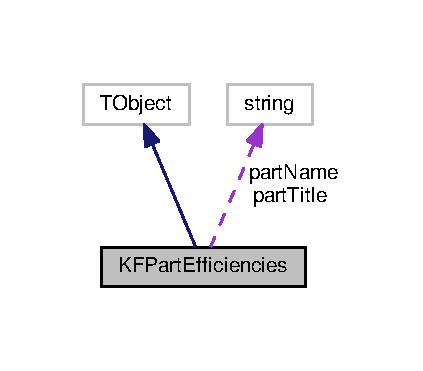
\includegraphics[width=203pt]{classKFPartEfficiencies__coll__graph}
\end{center}
\end{figure}
\subsection*{Public Member Functions}
\begin{DoxyCompactItemize}
\item 
\hyperlink{classKFPartEfficiencies_a0559adf38115aa40fc8fa96a7d2b2abd}{K\+F\+Part\+Efficiencies} ()\hypertarget{classKFPartEfficiencies_a0559adf38115aa40fc8fa96a7d2b2abd}{}\label{classKFPartEfficiencies_a0559adf38115aa40fc8fa96a7d2b2abd}

\begin{DoxyCompactList}\small\item\em The default constructor. Defines the list of decays to be analysed and their properties. Please, see the code for indexing scheme. \end{DoxyCompactList}\item 
int \hyperlink{classKFPartEfficiencies_a604060167fb04565e2311cffbe680250}{Get\+Particle\+Index} (int pdg)\hypertarget{classKFPartEfficiencies_a604060167fb04565e2311cffbe680250}{}\label{classKFPartEfficiencies_a604060167fb04565e2311cffbe680250}

\begin{DoxyCompactList}\small\item\em Returns index of the decay with a given P\+DG code in the scheme of the KF Particle Finder. If it is not present there -\/ returns \char`\"{}-\/1\char`\"{}. \end{DoxyCompactList}\item 
std\+::map$<$ int, int $>$ \hyperlink{classKFPartEfficiencies_a282d31782b56c5f15e7e73b9c3409048}{Get\+Pdg\+To\+Index\+Map} () const \hypertarget{classKFPartEfficiencies_a282d31782b56c5f15e7e73b9c3409048}{}\label{classKFPartEfficiencies_a282d31782b56c5f15e7e73b9c3409048}

\begin{DoxyCompactList}\small\item\em Returns the map between P\+DG codes and index of the decay in the scheme of the KF Particle Finder. \end{DoxyCompactList}\item 
virtual void \hyperlink{classKFPartEfficiencies_ad91a958383aeb2750786fc5c5c4c9d22}{Add\+Counter} (std\+::string shortname, std\+::string name)
\item 
\hyperlink{classKFPartEfficiencies}{K\+F\+Part\+Efficiencies} \& \hyperlink{classKFPartEfficiencies_a3659f3482cc8d1b25139740d3507690e}{operator+=} (\hyperlink{classKFPartEfficiencies}{K\+F\+Part\+Efficiencies} \&a)\hypertarget{classKFPartEfficiencies_a3659f3482cc8d1b25139740d3507690e}{}\label{classKFPartEfficiencies_a3659f3482cc8d1b25139740d3507690e}

\begin{DoxyCompactList}\small\item\em Operator to add efficiency table from object \char`\"{}a\char`\"{} to the current object. Returns the current object after addition. \end{DoxyCompactList}\item 
void \hyperlink{classKFPartEfficiencies_a171017b3a8cc125461be0dea84d8d99a}{Calc\+Eff} ()\hypertarget{classKFPartEfficiencies_a171017b3a8cc125461be0dea84d8d99a}{}\label{classKFPartEfficiencies_a171017b3a8cc125461be0dea84d8d99a}

\begin{DoxyCompactList}\small\item\em Function to calculate efficiency after all counters are set. If the counters are modified the function should be called again. \end{DoxyCompactList}\item 
void \hyperlink{classKFPartEfficiencies_ac5b13032d4d04564f696e0db9f544579}{Inc} (bool is\+Reco, int n\+Clones, bool is\+M\+C1, bool is\+M\+C2, bool is\+M\+C3, const std\+::string \&name)
\item 
void \hyperlink{classKFPartEfficiencies_a1ed4b9e456cafe92158ad43b9da1b816}{Inc\+Reco} (bool is\+Ghost, bool is\+Bg, const std\+::string \&name)
\item 
void \hyperlink{classKFPartEfficiencies_aae337f341af9595cd68f532e717e228a}{Print\+Eff} ()\hypertarget{classKFPartEfficiencies_aae337f341af9595cd68f532e717e228a}{}\label{classKFPartEfficiencies_aae337f341af9595cd68f532e717e228a}

\begin{DoxyCompactList}\small\item\em Prints the efficiency table on the screen. \end{DoxyCompactList}\item 
float \hyperlink{classKFPartEfficiencies_a6a48c0c6ded2a21062f73ba917229f6d}{Get\+Total4pi\+Efficiency} (int i\+Decay)\hypertarget{classKFPartEfficiencies_a6a48c0c6ded2a21062f73ba917229f6d}{}\label{classKFPartEfficiencies_a6a48c0c6ded2a21062f73ba917229f6d}

\begin{DoxyCompactList}\small\item\em Returns efficiency in 4pi for decay \char`\"{}i\+Decay\char`\"{}. \end{DoxyCompactList}\item 
float \hyperlink{classKFPartEfficiencies_ae896d8f2622dc6405584da3d4002eb40}{Get\+Total\+K\+F\+P\+Efficiency} (int i\+Decay)\hypertarget{classKFPartEfficiencies_ae896d8f2622dc6405584da3d4002eb40}{}\label{classKFPartEfficiencies_ae896d8f2622dc6405584da3d4002eb40}

\begin{DoxyCompactList}\small\item\em Returns efficiency of KF Particle Finder method (cuts) for decay \char`\"{}i\+Decay\char`\"{}. \end{DoxyCompactList}\item 
float \hyperlink{classKFPartEfficiencies_a19d7eac2141c53c0488d7f6f74b77efe}{Get\+Primary4pi\+Efficiency} (int i\+Decay)\hypertarget{classKFPartEfficiencies_a19d7eac2141c53c0488d7f6f74b77efe}{}\label{classKFPartEfficiencies_a19d7eac2141c53c0488d7f6f74b77efe}

\begin{DoxyCompactList}\small\item\em Returns efficiency in 4pi for decay \char`\"{}i\+Decay\char`\"{} for primary particles. \end{DoxyCompactList}\item 
float \hyperlink{classKFPartEfficiencies_afb1242e78db7e1132a850b3efc534c7f}{Get\+Primary\+K\+F\+P\+Efficiency} (int i\+Decay)\hypertarget{classKFPartEfficiencies_afb1242e78db7e1132a850b3efc534c7f}{}\label{classKFPartEfficiencies_afb1242e78db7e1132a850b3efc534c7f}

\begin{DoxyCompactList}\small\item\em Returns efficiency of KF Particle Finder method (cuts) for decay \char`\"{}i\+Decay\char`\"{} for primary particles. \end{DoxyCompactList}\item 
float \hyperlink{classKFPartEfficiencies_a3ae8747e495793f9af5c9e2365f09172}{Get\+Secondary4pi\+Efficiency} (int i\+Decay)\hypertarget{classKFPartEfficiencies_a3ae8747e495793f9af5c9e2365f09172}{}\label{classKFPartEfficiencies_a3ae8747e495793f9af5c9e2365f09172}

\begin{DoxyCompactList}\small\item\em Returns efficiency in 4pi for decay \char`\"{}i\+Decay\char`\"{} for secondary particles. \end{DoxyCompactList}\item 
float \hyperlink{classKFPartEfficiencies_a52c037d748cf6676c9c7d9aab71f9a0d}{Get\+Secondary\+K\+F\+P\+Efficiency} (int i\+Decay)\hypertarget{classKFPartEfficiencies_a52c037d748cf6676c9c7d9aab71f9a0d}{}\label{classKFPartEfficiencies_a52c037d748cf6676c9c7d9aab71f9a0d}

\begin{DoxyCompactList}\small\item\em Returns efficiency of KF Particle Finder method (cuts) for decay \char`\"{}i\+Decay\char`\"{} for secondary particles. \end{DoxyCompactList}\item 
void \hyperlink{classKFPartEfficiencies_ae4a38efd79dd905f6d0e82062ce4a966}{Add\+From\+File} (const std\+::string \&file\+Name)\hypertarget{classKFPartEfficiencies_ae4a38efd79dd905f6d0e82062ce4a966}{}\label{classKFPartEfficiencies_ae4a38efd79dd905f6d0e82062ce4a966}

\begin{DoxyCompactList}\small\item\em Adds efficiency from the file with the name defined by \char`\"{}file\+Name\char`\"{} to the current objects. \end{DoxyCompactList}\item 
int \hyperlink{classKFPartEfficiencies_a5119b5c564e1ccc597181711ba241ca7}{Get\+N\+Daughters} (int i\+Particle) const \hypertarget{classKFPartEfficiencies_a5119b5c564e1ccc597181711ba241ca7}{}\label{classKFPartEfficiencies_a5119b5c564e1ccc597181711ba241ca7}

\begin{DoxyCompactList}\small\item\em Returns number of daughter particles for the decay with index \char`\"{}i\+Particle\char`\"{}. \end{DoxyCompactList}\item 
int \hyperlink{classKFPartEfficiencies_a5865d2d8022ffe45914511992a0af079}{Get\+Daughter\+P\+DG} (int i\+Particle, int i\+Daughter) const \hypertarget{classKFPartEfficiencies_a5865d2d8022ffe45914511992a0af079}{}\label{classKFPartEfficiencies_a5865d2d8022ffe45914511992a0af079}

\begin{DoxyCompactList}\small\item\em Returns the P\+DG code of the daughter \char`\"{}i\+Daughter\char`\"{} from the decay with index \char`\"{}i\+Particle\char`\"{}. \end{DoxyCompactList}\item 
float \hyperlink{classKFPartEfficiencies_ace9d9cf07aefb8e523ac1ec6b1bdcab0}{Get\+Mass} (int i\+Particle) const \hypertarget{classKFPartEfficiencies_ace9d9cf07aefb8e523ac1ec6b1bdcab0}{}\label{classKFPartEfficiencies_ace9d9cf07aefb8e523ac1ec6b1bdcab0}

\begin{DoxyCompactList}\small\item\em Returns the table mass of the decay with index \char`\"{}i\+Particle\char`\"{}. \end{DoxyCompactList}\item 
float \hyperlink{classKFPartEfficiencies_a9f6f8e28db6c1692b0ee9415c8e63c03}{Get\+Mass\+Sigma} (int i\+Particle) const \hypertarget{classKFPartEfficiencies_a9f6f8e28db6c1692b0ee9415c8e63c03}{}\label{classKFPartEfficiencies_a9f6f8e28db6c1692b0ee9415c8e63c03}

\begin{DoxyCompactList}\small\item\em Returns expected width of the mass peak of the decay with index \char`\"{}i\+Particle\char`\"{}. \end{DoxyCompactList}\end{DoxyCompactItemize}
\subsection*{Public Attributes}
\begin{DoxyCompactItemize}
\item 
int \hyperlink{classKFPartEfficiencies_a1e94d7125c8ee9f06cbfd81ff9cf3ffe}{part\+P\+DG} \mbox{[}\hyperlink{classKFPartEfficiencies_a229165eeecbc664b7723d3ce588783e8}{n\+Particles}\mbox{]}\hypertarget{classKFPartEfficiencies_a1e94d7125c8ee9f06cbfd81ff9cf3ffe}{}\label{classKFPartEfficiencies_a1e94d7125c8ee9f06cbfd81ff9cf3ffe}

\begin{DoxyCompactList}\small\item\em Array of P\+DG codes assigned to the decays. \end{DoxyCompactList}\item 
std\+::string \hyperlink{classKFPartEfficiencies_a93c53aece9a458b82f3a87a1b2dfc386}{part\+Name} \mbox{[}\hyperlink{classKFPartEfficiencies_a229165eeecbc664b7723d3ce588783e8}{n\+Particles}\mbox{]}\hypertarget{classKFPartEfficiencies_a93c53aece9a458b82f3a87a1b2dfc386}{}\label{classKFPartEfficiencies_a93c53aece9a458b82f3a87a1b2dfc386}

\begin{DoxyCompactList}\small\item\em Array of names of the decay in the file with histograms. \end{DoxyCompactList}\item 
std\+::string \hyperlink{classKFPartEfficiencies_ae325b82a6db6f38f7a37af090c9ffc09}{part\+Title} \mbox{[}\hyperlink{classKFPartEfficiencies_a229165eeecbc664b7723d3ce588783e8}{n\+Particles}\mbox{]}\hypertarget{classKFPartEfficiencies_ae325b82a6db6f38f7a37af090c9ffc09}{}\label{classKFPartEfficiencies_ae325b82a6db6f38f7a37af090c9ffc09}

\begin{DoxyCompactList}\small\item\em Array of names of the decay in the output table with efficiency. \end{DoxyCompactList}\item 
std\+::vector$<$ std\+::vector$<$ int $>$ $>$ \hyperlink{classKFPartEfficiencies_abd5490c443f3a36eeff06523e04a2e8b}{part\+Daughter\+Pdg}\hypertarget{classKFPartEfficiencies_abd5490c443f3a36eeff06523e04a2e8b}{}\label{classKFPartEfficiencies_abd5490c443f3a36eeff06523e04a2e8b}

\begin{DoxyCompactList}\small\item\em Array with vectors of daughter particles for each decay. \end{DoxyCompactList}\item 
float \hyperlink{classKFPartEfficiencies_a48950848b5b2c8990a30d4dc58f2f0ec}{part\+M\+Histo\+Min} \mbox{[}\hyperlink{classKFPartEfficiencies_a229165eeecbc664b7723d3ce588783e8}{n\+Particles}\mbox{]}\hypertarget{classKFPartEfficiencies_a48950848b5b2c8990a30d4dc58f2f0ec}{}\label{classKFPartEfficiencies_a48950848b5b2c8990a30d4dc58f2f0ec}

\begin{DoxyCompactList}\small\item\em Array with lower boundary in the mass histograms for each decay. \end{DoxyCompactList}\item 
float \hyperlink{classKFPartEfficiencies_ad104f05f0cb7cf8cc6dd10e009a6bd65}{part\+M\+Histo\+Max} \mbox{[}\hyperlink{classKFPartEfficiencies_a229165eeecbc664b7723d3ce588783e8}{n\+Particles}\mbox{]}\hypertarget{classKFPartEfficiencies_ad104f05f0cb7cf8cc6dd10e009a6bd65}{}\label{classKFPartEfficiencies_ad104f05f0cb7cf8cc6dd10e009a6bd65}

\begin{DoxyCompactList}\small\item\em Array with upper boundary in the mass histograms for each decay. \end{DoxyCompactList}\item 
int \hyperlink{classKFPartEfficiencies_a55765f5f102fffd399b162ed2ccad4d2}{part\+Max\+Mult} \mbox{[}\hyperlink{classKFPartEfficiencies_a229165eeecbc664b7723d3ce588783e8}{n\+Particles}\mbox{]}\hypertarget{classKFPartEfficiencies_a55765f5f102fffd399b162ed2ccad4d2}{}\label{classKFPartEfficiencies_a55765f5f102fffd399b162ed2ccad4d2}

\begin{DoxyCompactList}\small\item\em Array with upper boundary in the multiplicity histograms of each decay. \end{DoxyCompactList}\item 
float \hyperlink{classKFPartEfficiencies_a652a5223c14c9d8e4a32c5203ce32d34}{part\+Mass} \mbox{[}\hyperlink{classKFPartEfficiencies_a229165eeecbc664b7723d3ce588783e8}{n\+Particles}\mbox{]}\hypertarget{classKFPartEfficiencies_a652a5223c14c9d8e4a32c5203ce32d34}{}\label{classKFPartEfficiencies_a652a5223c14c9d8e4a32c5203ce32d34}

\begin{DoxyCompactList}\small\item\em Array with table masses of each decay. \end{DoxyCompactList}\item 
float \hyperlink{classKFPartEfficiencies_a8d3d967e6832115dc711c33d6207c579}{part\+Life\+Time} \mbox{[}\hyperlink{classKFPartEfficiencies_a229165eeecbc664b7723d3ce588783e8}{n\+Particles}\mbox{]}\hypertarget{classKFPartEfficiencies_a8d3d967e6832115dc711c33d6207c579}{}\label{classKFPartEfficiencies_a8d3d967e6832115dc711c33d6207c579}

\begin{DoxyCompactList}\small\item\em Array with lifetimes in seconds of each decay. \end{DoxyCompactList}\item 
int \hyperlink{classKFPartEfficiencies_a3a6fae7d079f71634024028f88f9f1d7}{part\+Charge} \mbox{[}\hyperlink{classKFPartEfficiencies_a229165eeecbc664b7723d3ce588783e8}{n\+Particles}\mbox{]}\hypertarget{classKFPartEfficiencies_a3a6fae7d079f71634024028f88f9f1d7}{}\label{classKFPartEfficiencies_a3a6fae7d079f71634024028f88f9f1d7}

\begin{DoxyCompactList}\small\item\em Array with charge of each particle specie in units of the elementary charge. \end{DoxyCompactList}\item 
float \hyperlink{classKFPartEfficiencies_a915b3919e4055c50ba1ef2a44a40cd5d}{part\+Mass\+Sigma} \mbox{[}\hyperlink{classKFPartEfficiencies_a229165eeecbc664b7723d3ce588783e8}{n\+Particles}\mbox{]}\hypertarget{classKFPartEfficiencies_a915b3919e4055c50ba1ef2a44a40cd5d}{}\label{classKFPartEfficiencies_a915b3919e4055c50ba1ef2a44a40cd5d}

\begin{DoxyCompactList}\small\item\em Array with expected width of mass peaks used for the side band method. \end{DoxyCompactList}\end{DoxyCompactItemize}
\subsection*{Static Public Attributes}
\begin{DoxyCompactItemize}
\item 
static const int \hyperlink{classKFPartEfficiencies_a229165eeecbc664b7723d3ce588783e8}{n\+Particles} = 194\hypertarget{classKFPartEfficiencies_a229165eeecbc664b7723d3ce588783e8}{}\label{classKFPartEfficiencies_a229165eeecbc664b7723d3ce588783e8}

\begin{DoxyCompactList}\small\item\em Number of particles. \end{DoxyCompactList}\item 
static const int \hyperlink{classKFPartEfficiencies_a2c64f7d69d99fe6775db42741f55bbbe}{f\+First\+Hypernucleus\+Index} = 114\hypertarget{classKFPartEfficiencies_a2c64f7d69d99fe6775db42741f55bbbe}{}\label{classKFPartEfficiencies_a2c64f7d69d99fe6775db42741f55bbbe}

\begin{DoxyCompactList}\small\item\em Index of the first hypernuclei in the list. \end{DoxyCompactList}\item 
static const int \hyperlink{classKFPartEfficiencies_a0b4c54e513a38e19ada267f48affe056}{f\+Last\+Hypernucleus\+Index} = 130\hypertarget{classKFPartEfficiencies_a0b4c54e513a38e19ada267f48affe056}{}\label{classKFPartEfficiencies_a0b4c54e513a38e19ada267f48affe056}

\begin{DoxyCompactList}\small\item\em Index of the last hypernuclei in the list. \end{DoxyCompactList}\item 
static const int \hyperlink{classKFPartEfficiencies_a50c0554b3a82a0e0825451b97d8b7348}{f\+First\+Missing\+Mass\+Particle\+Index} = 131\hypertarget{classKFPartEfficiencies_a50c0554b3a82a0e0825451b97d8b7348}{}\label{classKFPartEfficiencies_a50c0554b3a82a0e0825451b97d8b7348}

\begin{DoxyCompactList}\small\item\em Index of the first decay reconstructed by the missing mass method. \end{DoxyCompactList}\item 
static const int \hyperlink{classKFPartEfficiencies_a1133cb34df9e58e2bdbc177e1761f5f2}{f\+Last\+Missing\+Mass\+Particle\+Index} = 166\hypertarget{classKFPartEfficiencies_a1133cb34df9e58e2bdbc177e1761f5f2}{}\label{classKFPartEfficiencies_a1133cb34df9e58e2bdbc177e1761f5f2}

\begin{DoxyCompactList}\small\item\em Index of the last decay reconstructed by the missing mass method. \end{DoxyCompactList}\item 
static const int \hyperlink{classKFPartEfficiencies_aa789fded121eb78a0d49505f9c58431c}{f\+First\+Stable\+Particle\+Index} = 167\hypertarget{classKFPartEfficiencies_aa789fded121eb78a0d49505f9c58431c}{}\label{classKFPartEfficiencies_aa789fded121eb78a0d49505f9c58431c}

\begin{DoxyCompactList}\small\item\em Index of the first stable particle in the list. \end{DoxyCompactList}\item 
static const int \hyperlink{classKFPartEfficiencies_a579eae22841ce1981c8aed97d316e7b8}{f\+Last\+Stable\+Particle\+Index} = 184\hypertarget{classKFPartEfficiencies_a579eae22841ce1981c8aed97d316e7b8}{}\label{classKFPartEfficiencies_a579eae22841ce1981c8aed97d316e7b8}

\begin{DoxyCompactList}\small\item\em Index of the last stable particle in the list. \end{DoxyCompactList}\end{DoxyCompactItemize}
\subsection*{Friends}
\begin{DoxyCompactItemize}
\item 
std\+::fstream \& \hyperlink{classKFPartEfficiencies_a903f9bf66d3cf46bcf72597e65c09aec}{operator$<$$<$} (std\+::fstream \&strm, \hyperlink{classKFPartEfficiencies}{K\+F\+Part\+Efficiencies} \&a)\hypertarget{classKFPartEfficiencies_a903f9bf66d3cf46bcf72597e65c09aec}{}\label{classKFPartEfficiencies_a903f9bf66d3cf46bcf72597e65c09aec}

\begin{DoxyCompactList}\small\item\em Operator to write efficiencies to file. \end{DoxyCompactList}\item 
std\+::fstream \& \hyperlink{classKFPartEfficiencies_a71e0bc1c241b95eca6f1a992761af178}{operator$>$$>$} (std\+::fstream \&strm, \hyperlink{classKFPartEfficiencies}{K\+F\+Part\+Efficiencies} \&a)\hypertarget{classKFPartEfficiencies_a71e0bc1c241b95eca6f1a992761af178}{}\label{classKFPartEfficiencies_a71e0bc1c241b95eca6f1a992761af178}

\begin{DoxyCompactList}\small\item\em Operator to read efficiencies from file. \end{DoxyCompactList}\end{DoxyCompactItemize}


\subsection{Detailed Description}
Class to calculate efficiency of KF Particle Finder. 

\begin{DoxyAuthor}{Author}
M.\+Zyzak, I.\+Kisel 
\end{DoxyAuthor}
\begin{DoxyDate}{Date}
05.\+02.\+2019 
\end{DoxyDate}
\begin{DoxyVersion}{Version}
1.\+0
\end{DoxyVersion}
The class has two main purposes\+:~\newline
1) Defines the list of decays to be analysed\+: a unique code of the decay, its mass, lifetime, a list of daughter particles, etc. See \hyperlink{classKFPartEfficiencies_a0559adf38115aa40fc8fa96a7d2b2abd}{K\+F\+Part\+Efficiencies\+::\+K\+F\+Part\+Efficiencies()} for more details.~\newline
2) It calculates reconstruction efficiency of the decays from the KF Particle Finder scheme.~\newline
Definitions\+:~\newline
background -\/ physics background, when daughter particle come from the real particle, but the pdg hypothesis is incorrect, for example, Lambda-\/$>$p pi will create a physics background for K0s if the proton is misidentified;~\newline
ghost -\/ combinatorial background, tracks do not form a real vertex;~\newline
clone -\/ a particle is reconstructed several times, for example, particle track is split into to parts due to the multiple scattering. 

\subsection{Member Function Documentation}
\index{K\+F\+Part\+Efficiencies@{K\+F\+Part\+Efficiencies}!Add\+Counter@{Add\+Counter}}
\index{Add\+Counter@{Add\+Counter}!K\+F\+Part\+Efficiencies@{K\+F\+Part\+Efficiencies}}
\subsubsection[{\texorpdfstring{Add\+Counter(std\+::string shortname, std\+::string name)}{AddCounter(std::string shortname, std::string name)}}]{\setlength{\rightskip}{0pt plus 5cm}virtual void K\+F\+Part\+Efficiencies\+::\+Add\+Counter (
\begin{DoxyParamCaption}
\item[{std\+::string}]{shortname, }
\item[{std\+::string}]{name}
\end{DoxyParamCaption}
)\hspace{0.3cm}{\ttfamily [inline]}, {\ttfamily [virtual]}}\hypertarget{classKFPartEfficiencies_ad91a958383aeb2750786fc5c5c4c9d22}{}\label{classKFPartEfficiencies_ad91a958383aeb2750786fc5c5c4c9d22}
Adds a counter with the name defined by \char`\"{}name\char`\"{} to all counter objects. For easiness of operation with counters, a shortname is assigned to each of them and the corresponding entry in the map indices is done. 
\begin{DoxyParams}[1]{Parameters}
\mbox{\tt in}  & {\em shortname} & -\/ a short name of the counter for fast and easy access to its index \\
\hline
\mbox{\tt in}  & {\em name} & -\/ name of the counter which is added to each counter object.\\
\hline
\end{DoxyParams}
\index{K\+F\+Part\+Efficiencies@{K\+F\+Part\+Efficiencies}!Inc@{Inc}}
\index{Inc@{Inc}!K\+F\+Part\+Efficiencies@{K\+F\+Part\+Efficiencies}}
\subsubsection[{\texorpdfstring{Inc(bool is\+Reco, int n\+Clones, bool is\+M\+C1, bool is\+M\+C2, bool is\+M\+C3, const std\+::string \&name)}{Inc(bool isReco, int nClones, bool isMC1, bool isMC2, bool isMC3, const std::string &name)}}]{\setlength{\rightskip}{0pt plus 5cm}void K\+F\+Part\+Efficiencies\+::\+Inc (
\begin{DoxyParamCaption}
\item[{bool}]{is\+Reco, }
\item[{int}]{n\+Clones, }
\item[{bool}]{is\+M\+C1, }
\item[{bool}]{is\+M\+C2, }
\item[{bool}]{is\+M\+C3, }
\item[{const std\+::string \&}]{name}
\end{DoxyParamCaption}
)\hspace{0.3cm}{\ttfamily [inline]}}\hypertarget{classKFPartEfficiencies_ac5b13032d4d04564f696e0db9f544579}{}\label{classKFPartEfficiencies_ac5b13032d4d04564f696e0db9f544579}
Increases counters by one, if the corresponding boolean variable is \char`\"{}true\char`\"{}. 
\begin{DoxyParams}[1]{Parameters}
\mbox{\tt in}  & {\em is\+Reco} & -\/ \char`\"{}true\char`\"{} if particle is reconstructed \\
\hline
\mbox{\tt in}  & {\em n\+Clones} & -\/ number of double reconstructed particles for the given MC particle, will be added to the \char`\"{}clone\char`\"{} counters \\
\hline
\mbox{\tt in}  & {\em is\+M\+C1} & -\/ \char`\"{}true\char`\"{} if particle is reconstructable in 4pi, mc1 is increased \\
\hline
\mbox{\tt in}  & {\em is\+M\+C2} & -\/ \char`\"{}true\char`\"{} if all daughters are reconstructable, mc2 is increased \\
\hline
\mbox{\tt in}  & {\em is\+M\+C3} & -\/ \char`\"{}true\char`\"{} if all daughters are reconstructed, mc3 is increased \\
\hline
\mbox{\tt in}  & {\em name} & -\/ \char`\"{}shortname\char`\"{} of the set of counters, which should be increased\\
\hline
\end{DoxyParams}
\index{K\+F\+Part\+Efficiencies@{K\+F\+Part\+Efficiencies}!Inc\+Reco@{Inc\+Reco}}
\index{Inc\+Reco@{Inc\+Reco}!K\+F\+Part\+Efficiencies@{K\+F\+Part\+Efficiencies}}
\subsubsection[{\texorpdfstring{Inc\+Reco(bool is\+Ghost, bool is\+Bg, const std\+::string \&name)}{IncReco(bool isGhost, bool isBg, const std::string &name)}}]{\setlength{\rightskip}{0pt plus 5cm}void K\+F\+Part\+Efficiencies\+::\+Inc\+Reco (
\begin{DoxyParamCaption}
\item[{bool}]{is\+Ghost, }
\item[{bool}]{is\+Bg, }
\item[{const std\+::string \&}]{name}
\end{DoxyParamCaption}
)\hspace{0.3cm}{\ttfamily [inline]}}\hypertarget{classKFPartEfficiencies_a1ed4b9e456cafe92158ad43b9da1b816}{}\label{classKFPartEfficiencies_a1ed4b9e456cafe92158ad43b9da1b816}
Increases counters by one, if the corresponding boolean variable is \char`\"{}true\char`\"{}. 
\begin{DoxyParams}[1]{Parameters}
\mbox{\tt in}  & {\em is\+Ghost} & -\/ \char`\"{}true\char`\"{} if ghost is added \\
\hline
\mbox{\tt in}  & {\em is\+Bg} & -\/ \char`\"{}true\char`\"{} if physics background is added \\
\hline
\mbox{\tt in}  & {\em name} & -\/ \char`\"{}shortname\char`\"{} of the set of counters, which should be increased\\
\hline
\end{DoxyParams}


The documentation for this class was generated from the following file\+:\begin{DoxyCompactItemize}
\item 
/home/user/cbmdir/kfpf/\+K\+F\+Particle/\+K\+F\+Particle\+Performance/K\+F\+Part\+Efficiencies.\+h\end{DoxyCompactItemize}

\hypertarget{classKFParticle}{}\section{K\+F\+Particle Class Reference}
\label{classKFParticle}\index{K\+F\+Particle@{K\+F\+Particle}}


The main scalar class of KF Particle package, describes particle objects.  




{\ttfamily \#include $<$K\+F\+Particle.\+h$>$}



Inheritance diagram for K\+F\+Particle\+:
\nopagebreak
\begin{figure}[H]
\begin{center}
\leavevmode
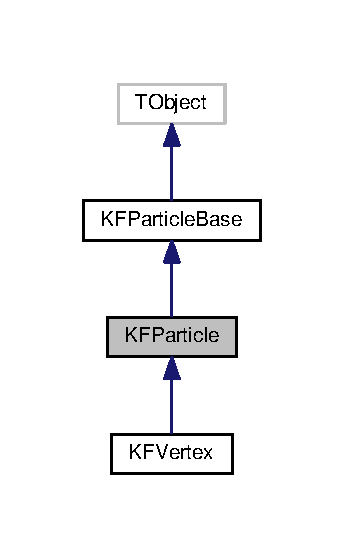
\includegraphics[width=165pt]{classKFParticle__inherit__graph}
\end{center}
\end{figure}


Collaboration diagram for K\+F\+Particle\+:
\nopagebreak
\begin{figure}[H]
\begin{center}
\leavevmode
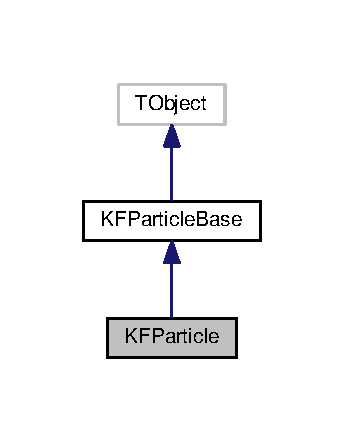
\includegraphics[width=165pt]{classKFParticle__coll__graph}
\end{center}
\end{figure}
\subsection*{Public Member Functions}
\begin{DoxyCompactItemize}
\item 
\hyperlink{classKFParticle_a68828423bef2ed7e280698a0cc5704c2}{K\+F\+Particle} (const \hyperlink{classKFParticle}{K\+F\+Particle} \&d1, const \hyperlink{classKFParticle}{K\+F\+Particle} \&d2)
\item 
\hyperlink{classKFParticle_ad77dfee950a5c9daa80efa08c84e85cb}{K\+F\+Particle} (const \hyperlink{classKFParticle}{K\+F\+Particle} \&d1, const \hyperlink{classKFParticle}{K\+F\+Particle} \&d2, const \hyperlink{classKFParticle}{K\+F\+Particle} \&d3)
\item 
\hyperlink{classKFParticle_a632873e701f93a69879afb7296dd6f40}{K\+F\+Particle} (const \hyperlink{classKFParticle}{K\+F\+Particle} \&d1, const \hyperlink{classKFParticle}{K\+F\+Particle} \&d2, const \hyperlink{classKFParticle}{K\+F\+Particle} \&d3, const \hyperlink{classKFParticle}{K\+F\+Particle} \&d4)
\item 
void \hyperlink{classKFParticle_a688e43bc457ac9cc866e7e4a86c64bed}{Create} (const float Param\mbox{[}$\,$\mbox{]}, const float Cov\mbox{[}$\,$\mbox{]}, Int\+\_\+t Charge, float mass)
\item 
void \hyperlink{classKFParticle_a01fe4b3048c5c5337565a9b3da127c3d}{Create} (const Double\+\_\+t Param\mbox{[}$\,$\mbox{]}, const Double\+\_\+t Cov\mbox{[}$\,$\mbox{]}, Int\+\_\+t Charge, float mass)
\item 
\hyperlink{classKFParticle_ae6c3f778dbbbd47cef6bd56cbf9ce714}{K\+F\+Particle} (const \hyperlink{classKFPTrack}{K\+F\+P\+Track} \&track, int P\+ID)
\item 
\hyperlink{classKFParticle_aadf37a45429b3683bee536e30300a404}{K\+F\+Particle} (const \hyperlink{classKFPVertex}{K\+F\+P\+Vertex} \&vertex)
\item 
Bool\+\_\+t \hyperlink{classKFParticle_a22358b18680f63474c0329163c13080e}{Get\+At\+Production\+Vertex} () const \hypertarget{classKFParticle_a22358b18680f63474c0329163c13080e}{}\label{classKFParticle_a22358b18680f63474c0329163c13080e}

\begin{DoxyCompactList}\small\item\em Returns a flag which shows if the particle is located at the production point. \end{DoxyCompactList}\item 
void \hyperlink{classKFParticle_a2a1c4001b07352ad6aa73065f502957a}{Set\+At\+Production\+Vertex} (Bool\+\_\+t b)\hypertarget{classKFParticle_a2a1c4001b07352ad6aa73065f502957a}{}\label{classKFParticle_a2a1c4001b07352ad6aa73065f502957a}

\begin{DoxyCompactList}\small\item\em Set a flag that particle is at the production point. \end{DoxyCompactList}\item 
float \hyperlink{classKFParticle_a79dce9fd75bb4fb4aba288ccf6c7eb66}{GetP} () const \hypertarget{classKFParticle_a79dce9fd75bb4fb4aba288ccf6c7eb66}{}\label{classKFParticle_a79dce9fd75bb4fb4aba288ccf6c7eb66}

\begin{DoxyCompactList}\small\item\em Returns momentum. \end{DoxyCompactList}\item 
float \hyperlink{classKFParticle_af84e1b54f8c1c707d5f99b9865843193}{Get\+Pt} () const \hypertarget{classKFParticle_af84e1b54f8c1c707d5f99b9865843193}{}\label{classKFParticle_af84e1b54f8c1c707d5f99b9865843193}

\begin{DoxyCompactList}\small\item\em Returns transverse momentum. \end{DoxyCompactList}\item 
float \hyperlink{classKFParticle_ae01bc73d12e613bc9ad51a378ff0e65a}{Get\+Eta} () const \hypertarget{classKFParticle_ae01bc73d12e613bc9ad51a378ff0e65a}{}\label{classKFParticle_ae01bc73d12e613bc9ad51a378ff0e65a}

\begin{DoxyCompactList}\small\item\em Returns pseudorapidity. \end{DoxyCompactList}\item 
float \hyperlink{classKFParticle_abad00287b0ea28ad7d502d0f2cfd02ca}{Get\+Phi} () const \hypertarget{classKFParticle_abad00287b0ea28ad7d502d0f2cfd02ca}{}\label{classKFParticle_abad00287b0ea28ad7d502d0f2cfd02ca}

\begin{DoxyCompactList}\small\item\em Returns the azimuthal angle phi. \end{DoxyCompactList}\item 
float \hyperlink{classKFParticle_a9b26df4f50340bd40cfd3f3fab0aee11}{Get\+Momentum} () const \hypertarget{classKFParticle_a9b26df4f50340bd40cfd3f3fab0aee11}{}\label{classKFParticle_a9b26df4f50340bd40cfd3f3fab0aee11}

\begin{DoxyCompactList}\small\item\em Returns momentum. \end{DoxyCompactList}\item 
float \hyperlink{classKFParticle_a373770508aea8198a204ae52071c3269}{Get\+Mass} () const \hypertarget{classKFParticle_a373770508aea8198a204ae52071c3269}{}\label{classKFParticle_a373770508aea8198a204ae52071c3269}

\begin{DoxyCompactList}\small\item\em Returns mass. \end{DoxyCompactList}\item 
float \hyperlink{classKFParticle_a34e5c0327a0c751be4b3e5d94f3e7397}{Get\+Decay\+Length} () const \hypertarget{classKFParticle_a34e5c0327a0c751be4b3e5d94f3e7397}{}\label{classKFParticle_a34e5c0327a0c751be4b3e5d94f3e7397}

\begin{DoxyCompactList}\small\item\em Returns decay length. \end{DoxyCompactList}\item 
float \hyperlink{classKFParticle_a4c93b7924e17f83fca4e60294322ce94}{Get\+Decay\+Length\+XY} () const \hypertarget{classKFParticle_a4c93b7924e17f83fca4e60294322ce94}{}\label{classKFParticle_a4c93b7924e17f83fca4e60294322ce94}

\begin{DoxyCompactList}\small\item\em Returns decay length in XY. \end{DoxyCompactList}\item 
float \hyperlink{classKFParticle_adaa76bf36576d161af9f1d31a54d4642}{Get\+Life\+Time} () const \hypertarget{classKFParticle_adaa76bf36576d161af9f1d31a54d4642}{}\label{classKFParticle_adaa76bf36576d161af9f1d31a54d4642}

\begin{DoxyCompactList}\small\item\em Returns life time ctau \mbox{[}cm\mbox{]}. \end{DoxyCompactList}\item 
float \hyperlink{classKFParticle_ad53e12b3f5e3ea5fe626f5da798ba6b1}{GetR} () const \hypertarget{classKFParticle_ad53e12b3f5e3ea5fe626f5da798ba6b1}{}\label{classKFParticle_ad53e12b3f5e3ea5fe626f5da798ba6b1}

\begin{DoxyCompactList}\small\item\em Returns distance to the origin of the coordinate system \{0,0,0\}. \end{DoxyCompactList}\item 
float \hyperlink{classKFParticle_a8dc2a3b77fce50215337e660085bf969}{Get\+ErrX} () const \hypertarget{classKFParticle_a8dc2a3b77fce50215337e660085bf969}{}\label{classKFParticle_a8dc2a3b77fce50215337e660085bf969}

\begin{DoxyCompactList}\small\item\em Returns the error of X of current position. \end{DoxyCompactList}\item 
float \hyperlink{classKFParticle_a3cc152ee00d5c702adb79dfeffb4739a}{Get\+ErrY} () const \hypertarget{classKFParticle_a3cc152ee00d5c702adb79dfeffb4739a}{}\label{classKFParticle_a3cc152ee00d5c702adb79dfeffb4739a}

\begin{DoxyCompactList}\small\item\em Returns the error of Y of current position. \end{DoxyCompactList}\item 
float \hyperlink{classKFParticle_ae1b33148a5b3bedff0ee24bacd73c9be}{Get\+ErrZ} () const \hypertarget{classKFParticle_ae1b33148a5b3bedff0ee24bacd73c9be}{}\label{classKFParticle_ae1b33148a5b3bedff0ee24bacd73c9be}

\begin{DoxyCompactList}\small\item\em Returns the error of Z of current position. \end{DoxyCompactList}\item 
float \hyperlink{classKFParticle_a658b4dc249b9d92c512183ab95f721ec}{Get\+Err\+Px} () const \hypertarget{classKFParticle_a658b4dc249b9d92c512183ab95f721ec}{}\label{classKFParticle_a658b4dc249b9d92c512183ab95f721ec}

\begin{DoxyCompactList}\small\item\em Returns the error of X-\/compoment of the particle momentum. \end{DoxyCompactList}\item 
float \hyperlink{classKFParticle_a49b8aff03c03c33d21e09c935f3839ae}{Get\+Err\+Py} () const \hypertarget{classKFParticle_a49b8aff03c03c33d21e09c935f3839ae}{}\label{classKFParticle_a49b8aff03c03c33d21e09c935f3839ae}

\begin{DoxyCompactList}\small\item\em Returns the error of Y-\/compoment of the particle momentum. \end{DoxyCompactList}\item 
float \hyperlink{classKFParticle_a91247862b37bb70805249fcb59f86f3a}{Get\+Err\+Pz} () const \hypertarget{classKFParticle_a91247862b37bb70805249fcb59f86f3a}{}\label{classKFParticle_a91247862b37bb70805249fcb59f86f3a}

\begin{DoxyCompactList}\small\item\em Returns the error of Z-\/compoment of the particle momentum. \end{DoxyCompactList}\item 
float \hyperlink{classKFParticle_a8ffaa29ff6ec0f700768fd28088c3d04}{Get\+ErrE} () const \hypertarget{classKFParticle_a8ffaa29ff6ec0f700768fd28088c3d04}{}\label{classKFParticle_a8ffaa29ff6ec0f700768fd28088c3d04}

\begin{DoxyCompactList}\small\item\em Returns the error of energy. \end{DoxyCompactList}\item 
float \hyperlink{classKFParticle_a517852a4d166a004343c9e2b64310115}{Get\+ErrS} () const \hypertarget{classKFParticle_a517852a4d166a004343c9e2b64310115}{}\label{classKFParticle_a517852a4d166a004343c9e2b64310115}

\begin{DoxyCompactList}\small\item\em Returns the error of decay length / momentum. \end{DoxyCompactList}\item 
float \hyperlink{classKFParticle_a1f9c64d313d84e688945d119de4024a0}{Get\+ErrP} () const \hypertarget{classKFParticle_a1f9c64d313d84e688945d119de4024a0}{}\label{classKFParticle_a1f9c64d313d84e688945d119de4024a0}

\begin{DoxyCompactList}\small\item\em Returns the error of momentum. \end{DoxyCompactList}\item 
float \hyperlink{classKFParticle_a2521f48c4ee6207b31af48a72fbe1598}{Get\+Err\+Pt} () const \hypertarget{classKFParticle_a2521f48c4ee6207b31af48a72fbe1598}{}\label{classKFParticle_a2521f48c4ee6207b31af48a72fbe1598}

\begin{DoxyCompactList}\small\item\em Returns the error of transverse momentum. \end{DoxyCompactList}\item 
float \hyperlink{classKFParticle_a6e91734dc4f0c0edac14d43f8bf9ffd5}{Get\+Err\+Eta} () const \hypertarget{classKFParticle_a6e91734dc4f0c0edac14d43f8bf9ffd5}{}\label{classKFParticle_a6e91734dc4f0c0edac14d43f8bf9ffd5}

\begin{DoxyCompactList}\small\item\em Returns the error of pseudorapidity. \end{DoxyCompactList}\item 
float \hyperlink{classKFParticle_a8ad31ee7426a8e5e7c7006e1880707be}{Get\+Err\+Phi} () const \hypertarget{classKFParticle_a8ad31ee7426a8e5e7c7006e1880707be}{}\label{classKFParticle_a8ad31ee7426a8e5e7c7006e1880707be}

\begin{DoxyCompactList}\small\item\em Returns the error of the azimuthal angle phi. \end{DoxyCompactList}\item 
float \hyperlink{classKFParticle_ad635dc5751c6d86728cb26a6ac5f2a01}{Get\+Err\+Momentum} () const \hypertarget{classKFParticle_ad635dc5751c6d86728cb26a6ac5f2a01}{}\label{classKFParticle_ad635dc5751c6d86728cb26a6ac5f2a01}

\begin{DoxyCompactList}\small\item\em Returns the error of momentum. \end{DoxyCompactList}\item 
float \hyperlink{classKFParticle_a719c0871275fe63f83645fa4baff3720}{Get\+Err\+Mass} () const \hypertarget{classKFParticle_a719c0871275fe63f83645fa4baff3720}{}\label{classKFParticle_a719c0871275fe63f83645fa4baff3720}

\begin{DoxyCompactList}\small\item\em Returns the error of mass. \end{DoxyCompactList}\item 
float \hyperlink{classKFParticle_a5d1593128ff34775e02c91b1e23fdd6f}{Get\+Err\+Decay\+Length} () const \hypertarget{classKFParticle_a5d1593128ff34775e02c91b1e23fdd6f}{}\label{classKFParticle_a5d1593128ff34775e02c91b1e23fdd6f}

\begin{DoxyCompactList}\small\item\em Returns the error of decay length. \end{DoxyCompactList}\item 
float \hyperlink{classKFParticle_af1ae37c8dbace5d6486fbce3d954d2d9}{Get\+Err\+Decay\+Length\+XY} () const \hypertarget{classKFParticle_af1ae37c8dbace5d6486fbce3d954d2d9}{}\label{classKFParticle_af1ae37c8dbace5d6486fbce3d954d2d9}

\begin{DoxyCompactList}\small\item\em Returns the error of decay length in XY. \end{DoxyCompactList}\item 
float \hyperlink{classKFParticle_a28e29b46104f3e96c2923ba0204d1c08}{Get\+Err\+Life\+Time} () const \hypertarget{classKFParticle_a28e29b46104f3e96c2923ba0204d1c08}{}\label{classKFParticle_a28e29b46104f3e96c2923ba0204d1c08}

\begin{DoxyCompactList}\small\item\em Returns the error of life time. \end{DoxyCompactList}\item 
float \hyperlink{classKFParticle_ae1336ce640e8364c95d9ec2ce0e0ed09}{Get\+ErrR} () const \hypertarget{classKFParticle_ae1336ce640e8364c95d9ec2ce0e0ed09}{}\label{classKFParticle_ae1336ce640e8364c95d9ec2ce0e0ed09}

\begin{DoxyCompactList}\small\item\em Returns the error of distance to the origin of the coordinate system \{0,0,0\}. \end{DoxyCompactList}\item 
int \hyperlink{classKFParticle_ac0c1bc6b565ecd917f2a9330f41cfe5d}{GetP} (float \&P, float \&SigmaP) const 
\item 
int \hyperlink{classKFParticle_a9c96532cca6b59748d3f0aec654a8222}{Get\+Pt} (float \&Pt, float \&Sigma\+Pt) const 
\item 
int \hyperlink{classKFParticle_acd6ab4335bdb19e5a19d5c8fbbce05d5}{Get\+Eta} (float \&Eta, float \&Sigma\+Eta) const 
\item 
int \hyperlink{classKFParticle_ad7fa64af32317b896b88b0d52a150e3e}{Get\+Phi} (float \&Phi, float \&Sigma\+Phi) const 
\item 
int \hyperlink{classKFParticle_ab56906105509354096f21b23e29f7c5d}{Get\+Momentum} (float \&P, float \&SigmaP) const 
\item 
int \hyperlink{classKFParticle_ac01d70176620a48b72b3055ba077b14b}{Get\+Mass} (float \&M, float \&SigmaM) const 
\item 
int \hyperlink{classKFParticle_afa35ea1e264003c5d9fb6156ffed0ce7}{Get\+Decay\+Length} (float \&L, float \&SigmaL) const 
\item 
int \hyperlink{classKFParticle_a7c7b8430c20031c4dd76bbf61b436c5f}{Get\+Decay\+Length\+XY} (float \&L, float \&SigmaL) const 
\item 
int \hyperlink{classKFParticle_a8940d04d0f1535747fc6b075c57d749e}{Get\+Life\+Time} (float \&T, float \&SigmaT) const 
\item 
int \hyperlink{classKFParticle_a66ecc36b47a517f64857d86b5d9b9364}{GetR} (float \&R, float \&SigmaR) const 
\item 
float \hyperlink{classKFParticle_a95ca9088ad71a47c08d17012f161a0ed}{Get\+Rapidity} () const \hypertarget{classKFParticle_a95ca9088ad71a47c08d17012f161a0ed}{}\label{classKFParticle_a95ca9088ad71a47c08d17012f161a0ed}

\begin{DoxyCompactList}\small\item\em Returns rapidity of the particle. \end{DoxyCompactList}\item 
float \hyperlink{classKFParticle_a887de78bd509e9cc0d09fe03fcd22f7d}{Get\+Theta} () const \hypertarget{classKFParticle_a887de78bd509e9cc0d09fe03fcd22f7d}{}\label{classKFParticle_a887de78bd509e9cc0d09fe03fcd22f7d}

\begin{DoxyCompactList}\small\item\em Returns the polar angle in RZ. \end{DoxyCompactList}\item 
float $\ast$ \hyperlink{classKFParticle_a25172df44e982a6d08879a9638ca9b07}{Parameters} ()\hypertarget{classKFParticle_a25172df44e982a6d08879a9638ca9b07}{}\label{classKFParticle_a25172df44e982a6d08879a9638ca9b07}

\begin{DoxyCompactList}\small\item\em Returns pointer to the parameters fP. \end{DoxyCompactList}\item 
float $\ast$ \hyperlink{classKFParticle_ae577c154da7700d54d2300dd344b9130}{Covariance\+Matrix} ()\hypertarget{classKFParticle_ae577c154da7700d54d2300dd344b9130}{}\label{classKFParticle_ae577c154da7700d54d2300dd344b9130}

\begin{DoxyCompactList}\small\item\em Returns pointer to the covariance matrix fC. \end{DoxyCompactList}\item 
void \hyperlink{classKFParticle_a07fc58ec0483c40d870ff1162d9e6a1d}{Add\+Daughter} (const \hyperlink{classKFParticle}{K\+F\+Particle} \&Daughter)
\item 
void \hyperlink{classKFParticle_adc75a098f1e5e4fe4e322715a8227be8}{operator+=} (const \hyperlink{classKFParticle}{K\+F\+Particle} \&Daughter)
\item 
void \hyperlink{classKFParticle_ac336c1fd04ed435827dc29e684beb906}{Construct} (const \hyperlink{classKFParticle}{K\+F\+Particle} $\ast$v\+Daughters\mbox{[}$\,$\mbox{]}, int n\+Daughters, const \hyperlink{classKFParticle}{K\+F\+Particle} $\ast$Prod\+Vtx=nullptr, float Mass=-\/1)
\item 
void \hyperlink{classKFParticle_ae3e9fe6655354f5cb043eb36639f6d65}{Transport\+To\+Point} (const float xyz\mbox{[}$\,$\mbox{]})
\item 
void \hyperlink{classKFParticle_a809cab20c82d4e5e58ed6d2f6913d14f}{Transport\+To\+Particle} (const \hyperlink{classKFParticle}{K\+F\+Particle} \&p)
\item 
float \hyperlink{classKFParticle_af0e557256a15e60b0e3873490267b20f}{Get\+D\+Sto\+Point} (const float xyz\mbox{[}3\mbox{]}, float dsdr\mbox{[}6\mbox{]}) const 
\item 
void \hyperlink{classKFParticle_a1dfa2f6c4ec75c76a1b2aae35c05cae7}{Get\+D\+Sto\+Particle} (const \hyperlink{classKFParticleBase}{K\+F\+Particle\+Base} \&p, float dS\mbox{[}2\mbox{]}, float dsdr\mbox{[}4\mbox{]}\mbox{[}6\mbox{]}) const 
\item 
Bool\+\_\+t \hyperlink{classKFParticle_aa046ed0c434f62751066884405e1b380}{Get\+Distance\+From\+Vertex\+XY} (const float vtx\mbox{[}$\,$\mbox{]}, float \&val, float \&err) const 
\item 
Bool\+\_\+t \hyperlink{classKFParticle_a23612b32d0f5c8002731de325512843b}{Get\+Distance\+From\+Vertex\+XY} (const float vtx\mbox{[}$\,$\mbox{]}, const float Cv\mbox{[}$\,$\mbox{]}, float \&val, float \&err) const 
\item 
Bool\+\_\+t \hyperlink{classKFParticle_aa58e122337df9c2eb1bce3cca94b97ae}{Get\+Distance\+From\+Vertex\+XY} (const \hyperlink{classKFParticle}{K\+F\+Particle} \&Vtx, float \&val, float \&err) const 
\item 
float \hyperlink{classKFParticle_a2eb880056d6719b78e38a2027c32b0e9}{Get\+Distance\+From\+Vertex\+XY} (const float vtx\mbox{[}$\,$\mbox{]}) const 
\item 
float \hyperlink{classKFParticle_a204fe1adf6462b2baa8252cdb68e02f6}{Get\+Distance\+From\+Vertex\+XY} (const \hyperlink{classKFParticle}{K\+F\+Particle} \&Vtx) const 
\item 
float \hyperlink{classKFParticle_a70201c84649ebcbe60bddc5fb8a40e82}{Get\+Distance\+From\+Particle\+XY} (const \hyperlink{classKFParticle}{K\+F\+Particle} \&p) const 
\item 
float \hyperlink{classKFParticle_a08a4ff3f7c5034a431663bf016afc80f}{Get\+Deviation\+From\+Vertex\+XY} (const float v\mbox{[}$\,$\mbox{]}, const float Cv\mbox{[}$\,$\mbox{]}=nullptr) const 
\item 
float \hyperlink{classKFParticle_a40f3c5fe862d46e27a0e26947eb6ffa8}{Get\+Deviation\+From\+Vertex\+XY} (const \hyperlink{classKFParticle}{K\+F\+Particle} \&Vtx) const 
\item 
float \hyperlink{classKFParticle_a47d3c37061b44cea9558b2c5efb196c8}{Get\+Deviation\+From\+Particle\+XY} (const \hyperlink{classKFParticle}{K\+F\+Particle} \&p) const 
\item 
void \hyperlink{classKFParticle_aaf8fa9176455e4b34628568d33276069}{Get\+Parameters\+At\+Point} (const float $\ast$point, const float $\ast$point\+Cov, float $\ast$m, float $\ast$mV)
\item 
float \hyperlink{classKFParticle_a8dc18521243e2042e4aec0d5f821bac8}{Get\+Angle} (const \hyperlink{classKFParticle}{K\+F\+Particle} \&p) const 
\item 
float \hyperlink{classKFParticle_a8d4e9e9471f7bf3af01c637b28f7653c}{Get\+Angle\+XY} (const \hyperlink{classKFParticle}{K\+F\+Particle} \&p) const 
\item 
float \hyperlink{classKFParticle_aae77af43f2d9a88ff8dd7b80c65d44cb}{Get\+Angle\+RZ} (const \hyperlink{classKFParticle}{K\+F\+Particle} \&p) const 
\item 
float \hyperlink{classKFParticle_a7eb8965f66ac808147a95b27dc7162e9}{Get\+Pseudo\+Proper\+Decay\+Time} (const \hyperlink{classKFParticle}{K\+F\+Particle} \&prim\+Vertex, const float \&mass, float $\ast$time\+Err2=nullptr) const 
\item 
void \hyperlink{classKFParticle_a586922b2bf23f335bf999f50ff5d633f}{Get\+Field\+Value} (const float xyz\mbox{[}$\,$\mbox{]}, float B\mbox{[}$\,$\mbox{]}) const 
\item 
void \hyperlink{classKFParticle_a62f4f92c046f9690260b22fce67307e7}{Transport} (float dS, const float $\ast$dsdr, float P\mbox{[}$\,$\mbox{]}, float C\mbox{[}$\,$\mbox{]}, float $\ast$dsdr1=nullptr, float $\ast$F=nullptr, float $\ast$F1=nullptr) const 
\end{DoxyCompactItemize}
\subsection*{Additional Inherited Members}


\subsection{Detailed Description}
The main scalar class of KF Particle package, describes particle objects. 

\begin{DoxyAuthor}{Author}
S.\+Gorbunov, I.\+Kisel, M.\+Zyzak 
\end{DoxyAuthor}
\begin{DoxyDate}{Date}
05.\+02.\+2019 
\end{DoxyDate}
\begin{DoxyVersion}{Version}
1.\+0
\end{DoxyVersion}
The main scalar class of KF Particle pacakge, describes particle objects. The particle is described with the state vector \{ X, Y, Z, Px, Py, Pz, E \} and the corresponding covariance matrix. It contains functionality to create particle-\/object from track, to construct short-\/lived particles from other tracks or particles. The mathematics is based on the Kalman filter method. It also allows to subtract particles from the already constructed object, to transport particles, get parameters together with their errors, get distance to other particles and vertices, get deviations from them in terms of errors, etc. 

\subsection{Constructor \& Destructor Documentation}
\index{K\+F\+Particle@{K\+F\+Particle}!K\+F\+Particle@{K\+F\+Particle}}
\index{K\+F\+Particle@{K\+F\+Particle}!K\+F\+Particle@{K\+F\+Particle}}
\subsubsection[{\texorpdfstring{K\+F\+Particle(const K\+F\+Particle \&d1, const K\+F\+Particle \&d2)}{KFParticle(const KFParticle &d1, const KFParticle &d2)}}]{\setlength{\rightskip}{0pt plus 5cm}K\+F\+Particle\+::\+K\+F\+Particle (
\begin{DoxyParamCaption}
\item[{const {\bf K\+F\+Particle} \&}]{d1, }
\item[{const {\bf K\+F\+Particle} \&}]{d2}
\end{DoxyParamCaption}
)}\hypertarget{classKFParticle_a68828423bef2ed7e280698a0cc5704c2}{}\label{classKFParticle_a68828423bef2ed7e280698a0cc5704c2}
Constructs a particle from two input daughter particles 
\begin{DoxyParams}[1]{Parameters}
\mbox{\tt in}  & {\em d1} & -\/ the first daughter particle \\
\hline
\mbox{\tt in}  & {\em d2} & -\/ the second daughter particle\\
\hline
\end{DoxyParams}
\index{K\+F\+Particle@{K\+F\+Particle}!K\+F\+Particle@{K\+F\+Particle}}
\index{K\+F\+Particle@{K\+F\+Particle}!K\+F\+Particle@{K\+F\+Particle}}
\subsubsection[{\texorpdfstring{K\+F\+Particle(const K\+F\+Particle \&d1, const K\+F\+Particle \&d2, const K\+F\+Particle \&d3)}{KFParticle(const KFParticle &d1, const KFParticle &d2, const KFParticle &d3)}}]{\setlength{\rightskip}{0pt plus 5cm}K\+F\+Particle\+::\+K\+F\+Particle (
\begin{DoxyParamCaption}
\item[{const {\bf K\+F\+Particle} \&}]{d1, }
\item[{const {\bf K\+F\+Particle} \&}]{d2, }
\item[{const {\bf K\+F\+Particle} \&}]{d3}
\end{DoxyParamCaption}
)\hspace{0.3cm}{\ttfamily [inline]}}\hypertarget{classKFParticle_ad77dfee950a5c9daa80efa08c84e85cb}{}\label{classKFParticle_ad77dfee950a5c9daa80efa08c84e85cb}
Constructs a particle from three input daughter particles 
\begin{DoxyParams}[1]{Parameters}
\mbox{\tt in}  & {\em d1} & -\/ the first daughter particle \\
\hline
\mbox{\tt in}  & {\em d2} & -\/ the second daughter particle \\
\hline
\mbox{\tt in}  & {\em d3} & -\/ the third daughter particle\\
\hline
\end{DoxyParams}
\index{K\+F\+Particle@{K\+F\+Particle}!K\+F\+Particle@{K\+F\+Particle}}
\index{K\+F\+Particle@{K\+F\+Particle}!K\+F\+Particle@{K\+F\+Particle}}
\subsubsection[{\texorpdfstring{K\+F\+Particle(const K\+F\+Particle \&d1, const K\+F\+Particle \&d2, const K\+F\+Particle \&d3, const K\+F\+Particle \&d4)}{KFParticle(const KFParticle &d1, const KFParticle &d2, const KFParticle &d3, const KFParticle &d4)}}]{\setlength{\rightskip}{0pt plus 5cm}K\+F\+Particle\+::\+K\+F\+Particle (
\begin{DoxyParamCaption}
\item[{const {\bf K\+F\+Particle} \&}]{d1, }
\item[{const {\bf K\+F\+Particle} \&}]{d2, }
\item[{const {\bf K\+F\+Particle} \&}]{d3, }
\item[{const {\bf K\+F\+Particle} \&}]{d4}
\end{DoxyParamCaption}
)\hspace{0.3cm}{\ttfamily [inline]}}\hypertarget{classKFParticle_a632873e701f93a69879afb7296dd6f40}{}\label{classKFParticle_a632873e701f93a69879afb7296dd6f40}
Constructs a particle from four input daughter particles 
\begin{DoxyParams}[1]{Parameters}
\mbox{\tt in}  & {\em d1} & -\/ the first daughter particle \\
\hline
\mbox{\tt in}  & {\em d2} & -\/ the second daughter particle \\
\hline
\mbox{\tt in}  & {\em d3} & -\/ the third daughter particle \\
\hline
\mbox{\tt in}  & {\em d4} & -\/ the fourth daughter particle\\
\hline
\end{DoxyParams}
\index{K\+F\+Particle@{K\+F\+Particle}!K\+F\+Particle@{K\+F\+Particle}}
\index{K\+F\+Particle@{K\+F\+Particle}!K\+F\+Particle@{K\+F\+Particle}}
\subsubsection[{\texorpdfstring{K\+F\+Particle(const K\+F\+P\+Track \&track, int P\+I\+D)}{KFParticle(const KFPTrack &track, int PID)}}]{\setlength{\rightskip}{0pt plus 5cm}K\+F\+Particle\+::\+K\+F\+Particle (
\begin{DoxyParamCaption}
\item[{const {\bf K\+F\+P\+Track} \&}]{track, }
\item[{int}]{P\+ID}
\end{DoxyParamCaption}
)}\hypertarget{classKFParticle_ae6c3f778dbbbd47cef6bd56cbf9ce714}{}\label{classKFParticle_ae6c3f778dbbbd47cef6bd56cbf9ce714}
Constructor from a track in the KF Particle format, P\+ID hypothesis should be provided 
\begin{DoxyParams}[1]{Parameters}
\mbox{\tt in}  & {\em track} & -\/ \hyperlink{classKFPTrack}{K\+F\+P\+Track} containing 6 parameters\+: \{ X, Y, Z, Px, Py, Pz \} and their errors \\
\hline
\mbox{\tt in}  & {\em P\+ID} & -\/ P\+ID hypothesis, needed to assign mass to a particle and calculate the energy\\
\hline
\end{DoxyParams}
\index{K\+F\+Particle@{K\+F\+Particle}!K\+F\+Particle@{K\+F\+Particle}}
\index{K\+F\+Particle@{K\+F\+Particle}!K\+F\+Particle@{K\+F\+Particle}}
\subsubsection[{\texorpdfstring{K\+F\+Particle(const K\+F\+P\+Vertex \&vertex)}{KFParticle(const KFPVertex &vertex)}}]{\setlength{\rightskip}{0pt plus 5cm}K\+F\+Particle\+::\+K\+F\+Particle (
\begin{DoxyParamCaption}
\item[{const {\bf K\+F\+P\+Vertex} \&}]{vertex}
\end{DoxyParamCaption}
)\hspace{0.3cm}{\ttfamily [explicit]}}\hypertarget{classKFParticle_aadf37a45429b3683bee536e30300a404}{}\label{classKFParticle_aadf37a45429b3683bee536e30300a404}
Constructor from a vertex in the KF Particle format 
\begin{DoxyParams}[1]{Parameters}
\mbox{\tt in}  & {\em vertex} & -\/ \hyperlink{classKFPVertex}{K\+F\+P\+Vertex} containing 3 parameters\+: \{ X, Y, Z \} and their errors\\
\hline
\end{DoxyParams}


\subsection{Member Function Documentation}
\index{K\+F\+Particle@{K\+F\+Particle}!Add\+Daughter@{Add\+Daughter}}
\index{Add\+Daughter@{Add\+Daughter}!K\+F\+Particle@{K\+F\+Particle}}
\subsubsection[{\texorpdfstring{Add\+Daughter(const K\+F\+Particle \&\+Daughter)}{AddDaughter(const KFParticle &Daughter)}}]{\setlength{\rightskip}{0pt plus 5cm}void K\+F\+Particle\+::\+Add\+Daughter (
\begin{DoxyParamCaption}
\item[{const {\bf K\+F\+Particle} \&}]{Daughter}
\end{DoxyParamCaption}
)\hspace{0.3cm}{\ttfamily [inline]}}\hypertarget{classKFParticle_a07fc58ec0483c40d870ff1162d9e6a1d}{}\label{classKFParticle_a07fc58ec0483c40d870ff1162d9e6a1d}
Adds daughter to the current particle. Depending on the selected construction method uses\+: ~\newline
1) Either simplifyed fast mathematics which consideres momentum and energy as independent variables and thus ignores constraint on the fixed mass (f\+Construct\+Method = 0). In this case the mass of the daughter particle can be corrupted when the constructed vertex is added as the measurement and the mass of the output short-\/lived particle can become unphysical -\/ smaller then the threshold. Implemented in the \hyperlink{classKFParticleBase_afe25065680801ce33287e480ca0534e4}{Add\+Daughter\+With\+Energy\+Fit()} function ~\newline
2) Or slower but correct mathematics which requires that the masses of daughter particles stays fixed in the construction process (f\+Construct\+Method = 2). Implemented in the \hyperlink{classKFParticleBase_a143d70c6bd591a3294c4c0f89c8edcda}{Add\+Daughter\+With\+Energy\+Fit\+M\+C()} function. 
\begin{DoxyParams}[1]{Parameters}
\mbox{\tt in}  & {\em Daughter} & -\/ the daughter particle\\
\hline
\end{DoxyParams}
\index{K\+F\+Particle@{K\+F\+Particle}!Construct@{Construct}}
\index{Construct@{Construct}!K\+F\+Particle@{K\+F\+Particle}}
\subsubsection[{\texorpdfstring{Construct(const K\+F\+Particle $\ast$v\+Daughters[], int n\+Daughters, const K\+F\+Particle $\ast$\+Prod\+Vtx=nullptr, float Mass=-\/1)}{Construct(const KFParticle *vDaughters[], int nDaughters, const KFParticle *ProdVtx=nullptr, float Mass=-1)}}]{\setlength{\rightskip}{0pt plus 5cm}void K\+F\+Particle\+::\+Construct (
\begin{DoxyParamCaption}
\item[{const {\bf K\+F\+Particle} $\ast$}]{v\+Daughters\mbox{[}$\,$\mbox{]}, }
\item[{int}]{n\+Daughters, }
\item[{const {\bf K\+F\+Particle} $\ast$}]{Prod\+Vtx = {\ttfamily nullptr}, }
\item[{float}]{Mass = {\ttfamily -\/1}}
\end{DoxyParamCaption}
)\hspace{0.3cm}{\ttfamily [inline]}}\hypertarget{classKFParticle_ac336c1fd04ed435827dc29e684beb906}{}\label{classKFParticle_ac336c1fd04ed435827dc29e684beb906}
Constructs a short-\/lived particle from a set of daughter particles\+:~\newline
1) all parameters of the \char`\"{}this\char`\"{} objects are initialised;~\newline
2) daughters are added one after another;~\newline
3) if Parent pointer is not null, the production vertex is set to it;~\newline
4) if Mass hypothesis $>$=0 the mass constraint is set. 
\begin{DoxyParams}[1]{Parameters}
\mbox{\tt in}  & {\em v\+Daughters} & -\/ array of daughter particles \\
\hline
\mbox{\tt in}  & {\em n\+Daughters} & -\/ number of daughter particles in the input array \\
\hline
\mbox{\tt in}  & {\em Parent} & -\/ optional parrent particle \\
\hline
\mbox{\tt in}  & {\em Mass} & -\/ optional mass hypothesis\\
\hline
\end{DoxyParams}
\index{K\+F\+Particle@{K\+F\+Particle}!Create@{Create}}
\index{Create@{Create}!K\+F\+Particle@{K\+F\+Particle}}
\subsubsection[{\texorpdfstring{Create(const float Param[], const float Cov[], Int\+\_\+t Charge, float mass)}{Create(const float Param[], const float Cov[], Int_t Charge, float mass)}}]{\setlength{\rightskip}{0pt plus 5cm}void K\+F\+Particle\+::\+Create (
\begin{DoxyParamCaption}
\item[{const float}]{Param\mbox{[}$\,$\mbox{]}, }
\item[{const float}]{Cov\mbox{[}$\,$\mbox{]}, }
\item[{Int\+\_\+t}]{Charge, }
\item[{float}]{mass}
\end{DoxyParamCaption}
)}\hypertarget{classKFParticle_a688e43bc457ac9cc866e7e4a86c64bed}{}\label{classKFParticle_a688e43bc457ac9cc866e7e4a86c64bed}
Constructor from a \char`\"{}cartesian\char`\"{} track, mass hypothesis should be provided 
\begin{DoxyParams}[1]{Parameters}
\mbox{\tt in}  & {\em Param\mbox{[}6\mbox{]}} & = \{ X, Y, Z, Px, Py, Pz \} -\/ position and momentum \\
\hline
\mbox{\tt in}  & {\em Cov\mbox{[}21\mbox{]}} & -\/ lower-\/triangular part of the covariance matrix\+:~\newline
\begin{DoxyVerb}          (  0  .  .  .  .  . )
          (  1  2  .  .  .  . )
Cov[21] = (  3  4  5  .  .  . )
          (  6  7  8  9  .  . )
          ( 10 11 12 13 14  . )
          ( 15 16 17 18 19 20 )
\end{DoxyVerb}
 \\
\hline
\mbox{\tt in}  & {\em Charge} & -\/ charge of the particle in elementary charge units \\
\hline
\mbox{\tt in}  & {\em mass} & -\/ the mass hypothesis\\
\hline
\end{DoxyParams}
\index{K\+F\+Particle@{K\+F\+Particle}!Create@{Create}}
\index{Create@{Create}!K\+F\+Particle@{K\+F\+Particle}}
\subsubsection[{\texorpdfstring{Create(const Double\+\_\+t Param[], const Double\+\_\+t Cov[], Int\+\_\+t Charge, float mass)}{Create(const Double_t Param[], const Double_t Cov[], Int_t Charge, float mass)}}]{\setlength{\rightskip}{0pt plus 5cm}void K\+F\+Particle\+::\+Create (
\begin{DoxyParamCaption}
\item[{const Double\+\_\+t}]{Param\mbox{[}$\,$\mbox{]}, }
\item[{const Double\+\_\+t}]{Cov\mbox{[}$\,$\mbox{]}, }
\item[{Int\+\_\+t}]{Charge, }
\item[{float}]{mass}
\end{DoxyParamCaption}
)}\hypertarget{classKFParticle_a01fe4b3048c5c5337565a9b3da127c3d}{}\label{classKFParticle_a01fe4b3048c5c5337565a9b3da127c3d}
Constructor from a \char`\"{}cartesian\char`\"{} track, mass hypothesis should be provided 
\begin{DoxyParams}[1]{Parameters}
\mbox{\tt in}  & {\em Param\mbox{[}6\mbox{]}} & = \{ X, Y, Z, Px, Py, Pz \} -\/ position and momentum \\
\hline
\mbox{\tt in}  & {\em Cov\mbox{[}21\mbox{]}} & -\/ lower-\/triangular part of the covariance matrix\+:~\newline
\begin{DoxyVerb}          (  0  .  .  .  .  . )
          (  1  2  .  .  .  . )
Cov[21] = (  3  4  5  .  .  . )
          (  6  7  8  9  .  . )
          ( 10 11 12 13 14  . )
          ( 15 16 17 18 19 20 )
\end{DoxyVerb}
 \\
\hline
\mbox{\tt in}  & {\em Charge} & -\/ charge of the particle in elementary charge units \\
\hline
\mbox{\tt in}  & {\em mass} & -\/ the mass hypothesis\\
\hline
\end{DoxyParams}
\index{K\+F\+Particle@{K\+F\+Particle}!Get\+Angle@{Get\+Angle}}
\index{Get\+Angle@{Get\+Angle}!K\+F\+Particle@{K\+F\+Particle}}
\subsubsection[{\texorpdfstring{Get\+Angle(const K\+F\+Particle \&p) const }{GetAngle(const KFParticle &p) const }}]{\setlength{\rightskip}{0pt plus 5cm}float K\+F\+Particle\+::\+Get\+Angle (
\begin{DoxyParamCaption}
\item[{const {\bf K\+F\+Particle} \&}]{p}
\end{DoxyParamCaption}
) const}\hypertarget{classKFParticle_a8dc18521243e2042e4aec0d5f821bac8}{}\label{classKFParticle_a8dc18521243e2042e4aec0d5f821bac8}
Returns the opening angle between the current and the second particle in 3D. 
\begin{DoxyParams}[1]{Parameters}
\mbox{\tt in}  & {\em p} & -\/ the second particle\\
\hline
\end{DoxyParams}
\index{K\+F\+Particle@{K\+F\+Particle}!Get\+Angle\+RZ@{Get\+Angle\+RZ}}
\index{Get\+Angle\+RZ@{Get\+Angle\+RZ}!K\+F\+Particle@{K\+F\+Particle}}
\subsubsection[{\texorpdfstring{Get\+Angle\+R\+Z(const K\+F\+Particle \&p) const }{GetAngleRZ(const KFParticle &p) const }}]{\setlength{\rightskip}{0pt plus 5cm}float K\+F\+Particle\+::\+Get\+Angle\+RZ (
\begin{DoxyParamCaption}
\item[{const {\bf K\+F\+Particle} \&}]{p}
\end{DoxyParamCaption}
) const}\hypertarget{classKFParticle_aae77af43f2d9a88ff8dd7b80c65d44cb}{}\label{classKFParticle_aae77af43f2d9a88ff8dd7b80c65d44cb}
Returns the opening angle between the current and the second particle in the RZ plane, R = sqrt(X$\ast$\+X+\+Y$\ast$Y). 
\begin{DoxyParams}[1]{Parameters}
\mbox{\tt in}  & {\em p} & -\/ the second particle\\
\hline
\end{DoxyParams}
\index{K\+F\+Particle@{K\+F\+Particle}!Get\+Angle\+XY@{Get\+Angle\+XY}}
\index{Get\+Angle\+XY@{Get\+Angle\+XY}!K\+F\+Particle@{K\+F\+Particle}}
\subsubsection[{\texorpdfstring{Get\+Angle\+X\+Y(const K\+F\+Particle \&p) const }{GetAngleXY(const KFParticle &p) const }}]{\setlength{\rightskip}{0pt plus 5cm}float K\+F\+Particle\+::\+Get\+Angle\+XY (
\begin{DoxyParamCaption}
\item[{const {\bf K\+F\+Particle} \&}]{p}
\end{DoxyParamCaption}
) const}\hypertarget{classKFParticle_a8d4e9e9471f7bf3af01c637b28f7653c}{}\label{classKFParticle_a8d4e9e9471f7bf3af01c637b28f7653c}
Returns the opening angle between the current and the second particle in the XY plane. 
\begin{DoxyParams}[1]{Parameters}
\mbox{\tt in}  & {\em p} & -\/ the second particle\\
\hline
\end{DoxyParams}
\index{K\+F\+Particle@{K\+F\+Particle}!Get\+Decay\+Length@{Get\+Decay\+Length}}
\index{Get\+Decay\+Length@{Get\+Decay\+Length}!K\+F\+Particle@{K\+F\+Particle}}
\subsubsection[{\texorpdfstring{Get\+Decay\+Length(float \&\+L, float \&\+Sigma\+L) const }{GetDecayLength(float &L, float &SigmaL) const }}]{\setlength{\rightskip}{0pt plus 5cm}int K\+F\+Particle\+::\+Get\+Decay\+Length (
\begin{DoxyParamCaption}
\item[{float \&}]{L, }
\item[{float \&}]{SigmaL}
\end{DoxyParamCaption}
) const\hspace{0.3cm}{\ttfamily [inline]}}\hypertarget{classKFParticle_afa35ea1e264003c5d9fb6156ffed0ce7}{}\label{classKFParticle_afa35ea1e264003c5d9fb6156ffed0ce7}
Calculates the decay length of the particle in the laboratory system and its error. If they are well defined returns 0, otherwise 1. The production point should be set before calling this function. 
\begin{DoxyParams}[1]{Parameters}
\mbox{\tt out}  & {\em L} & -\/ the decay length \\
\hline
\mbox{\tt out}  & {\em SigmaL} & -\/ its error\\
\hline
\end{DoxyParams}
\index{K\+F\+Particle@{K\+F\+Particle}!Get\+Decay\+Length\+XY@{Get\+Decay\+Length\+XY}}
\index{Get\+Decay\+Length\+XY@{Get\+Decay\+Length\+XY}!K\+F\+Particle@{K\+F\+Particle}}
\subsubsection[{\texorpdfstring{Get\+Decay\+Length\+X\+Y(float \&\+L, float \&\+Sigma\+L) const }{GetDecayLengthXY(float &L, float &SigmaL) const }}]{\setlength{\rightskip}{0pt plus 5cm}int K\+F\+Particle\+::\+Get\+Decay\+Length\+XY (
\begin{DoxyParamCaption}
\item[{float \&}]{L, }
\item[{float \&}]{SigmaL}
\end{DoxyParamCaption}
) const\hspace{0.3cm}{\ttfamily [inline]}}\hypertarget{classKFParticle_a7c7b8430c20031c4dd76bbf61b436c5f}{}\label{classKFParticle_a7c7b8430c20031c4dd76bbf61b436c5f}
Calculates the projection in the XY plane of the decay length of the particle in the laboratory system and its error. If they are well defined returns 0, otherwise 1. The production point should be set before calling this function. 
\begin{DoxyParams}[1]{Parameters}
\mbox{\tt out}  & {\em L} & -\/ the decay length \\
\hline
\mbox{\tt out}  & {\em SigmaL} & -\/ its error\\
\hline
\end{DoxyParams}
\index{K\+F\+Particle@{K\+F\+Particle}!Get\+Deviation\+From\+Particle\+XY@{Get\+Deviation\+From\+Particle\+XY}}
\index{Get\+Deviation\+From\+Particle\+XY@{Get\+Deviation\+From\+Particle\+XY}!K\+F\+Particle@{K\+F\+Particle}}
\subsubsection[{\texorpdfstring{Get\+Deviation\+From\+Particle\+X\+Y(const K\+F\+Particle \&p) const }{GetDeviationFromParticleXY(const KFParticle &p) const }}]{\setlength{\rightskip}{0pt plus 5cm}float K\+F\+Particle\+::\+Get\+Deviation\+From\+Particle\+XY (
\begin{DoxyParamCaption}
\item[{const {\bf K\+F\+Particle} \&}]{p}
\end{DoxyParamCaption}
) const}\hypertarget{classKFParticle_a47d3c37061b44cea9558b2c5efb196c8}{}\label{classKFParticle_a47d3c37061b44cea9558b2c5efb196c8}
Returns sqrt(Chi2/ndf) deviation from other particle in the XY plane. 
\begin{DoxyParams}[1]{Parameters}
\mbox{\tt in}  & {\em p} & -\/ the second particle\\
\hline
\end{DoxyParams}
\index{K\+F\+Particle@{K\+F\+Particle}!Get\+Deviation\+From\+Vertex\+XY@{Get\+Deviation\+From\+Vertex\+XY}}
\index{Get\+Deviation\+From\+Vertex\+XY@{Get\+Deviation\+From\+Vertex\+XY}!K\+F\+Particle@{K\+F\+Particle}}
\subsubsection[{\texorpdfstring{Get\+Deviation\+From\+Vertex\+X\+Y(const float v[], const float Cv[]=nullptr) const }{GetDeviationFromVertexXY(const float v[], const float Cv[]=nullptr) const }}]{\setlength{\rightskip}{0pt plus 5cm}float K\+F\+Particle\+::\+Get\+Deviation\+From\+Vertex\+XY (
\begin{DoxyParamCaption}
\item[{const float}]{v\mbox{[}$\,$\mbox{]}, }
\item[{const float}]{Cv\mbox{[}$\,$\mbox{]} = {\ttfamily nullptr}}
\end{DoxyParamCaption}
) const}\hypertarget{classKFParticle_a08a4ff3f7c5034a431663bf016afc80f}{}\label{classKFParticle_a08a4ff3f7c5034a431663bf016afc80f}
Returns sqrt(Chi2/ndf) deviation from the vertex in the XY plane. 
\begin{DoxyParams}[1]{Parameters}
\mbox{\tt in}  & {\em vtx\mbox{[}2\mbox{]}} & -\/ \{ X, Y \} coordinates of the vertex \\
\hline
\mbox{\tt in}  & {\em Cv\mbox{[}3\mbox{]}} & -\/ lower-\/triangular part of the covariance matrix of the vertex\\
\hline
\end{DoxyParams}
\index{K\+F\+Particle@{K\+F\+Particle}!Get\+Deviation\+From\+Vertex\+XY@{Get\+Deviation\+From\+Vertex\+XY}}
\index{Get\+Deviation\+From\+Vertex\+XY@{Get\+Deviation\+From\+Vertex\+XY}!K\+F\+Particle@{K\+F\+Particle}}
\subsubsection[{\texorpdfstring{Get\+Deviation\+From\+Vertex\+X\+Y(const K\+F\+Particle \&\+Vtx) const }{GetDeviationFromVertexXY(const KFParticle &Vtx) const }}]{\setlength{\rightskip}{0pt plus 5cm}float K\+F\+Particle\+::\+Get\+Deviation\+From\+Vertex\+XY (
\begin{DoxyParamCaption}
\item[{const {\bf K\+F\+Particle} \&}]{Vtx}
\end{DoxyParamCaption}
) const}\hypertarget{classKFParticle_a40f3c5fe862d46e27a0e26947eb6ffa8}{}\label{classKFParticle_a40f3c5fe862d46e27a0e26947eb6ffa8}
Returns sqrt(Chi2/ndf) deviation from the vertex in the \hyperlink{classKFParticle}{K\+F\+Particle} format in the XY plane. 
\begin{DoxyParams}[1]{Parameters}
\mbox{\tt in}  & {\em Vtx} & -\/ the vertex in the \hyperlink{classKFParticle}{K\+F\+Particle} format\\
\hline
\end{DoxyParams}
\index{K\+F\+Particle@{K\+F\+Particle}!Get\+Distance\+From\+Particle\+XY@{Get\+Distance\+From\+Particle\+XY}}
\index{Get\+Distance\+From\+Particle\+XY@{Get\+Distance\+From\+Particle\+XY}!K\+F\+Particle@{K\+F\+Particle}}
\subsubsection[{\texorpdfstring{Get\+Distance\+From\+Particle\+X\+Y(const K\+F\+Particle \&p) const }{GetDistanceFromParticleXY(const KFParticle &p) const }}]{\setlength{\rightskip}{0pt plus 5cm}float K\+F\+Particle\+::\+Get\+Distance\+From\+Particle\+XY (
\begin{DoxyParamCaption}
\item[{const {\bf K\+F\+Particle} \&}]{p}
\end{DoxyParamCaption}
) const}\hypertarget{classKFParticle_a70201c84649ebcbe60bddc5fb8a40e82}{}\label{classKFParticle_a70201c84649ebcbe60bddc5fb8a40e82}
Returns the D\+CA distance between the current and the second particles in the XY plane. 
\begin{DoxyParams}[1]{Parameters}
\mbox{\tt in}  & {\em p} & -\/ the second particle\\
\hline
\end{DoxyParams}
\index{K\+F\+Particle@{K\+F\+Particle}!Get\+Distance\+From\+Vertex\+XY@{Get\+Distance\+From\+Vertex\+XY}}
\index{Get\+Distance\+From\+Vertex\+XY@{Get\+Distance\+From\+Vertex\+XY}!K\+F\+Particle@{K\+F\+Particle}}
\subsubsection[{\texorpdfstring{Get\+Distance\+From\+Vertex\+X\+Y(const float vtx[], float \&val, float \&err) const }{GetDistanceFromVertexXY(const float vtx[], float &val, float &err) const }}]{\setlength{\rightskip}{0pt plus 5cm}Bool\+\_\+t K\+F\+Particle\+::\+Get\+Distance\+From\+Vertex\+XY (
\begin{DoxyParamCaption}
\item[{const float}]{vtx\mbox{[}$\,$\mbox{]}, }
\item[{float \&}]{val, }
\item[{float \&}]{err}
\end{DoxyParamCaption}
) const}\hypertarget{classKFParticle_aa046ed0c434f62751066884405e1b380}{}\label{classKFParticle_aa046ed0c434f62751066884405e1b380}
Calculates the D\+CA distance from a vertex together with the error in the XY plane. Returns \char`\"{}true\char`\"{} if calculation is failed, \char`\"{}false\char`\"{} if both value and the error are well defined. 
\begin{DoxyParams}[1]{Parameters}
\mbox{\tt in}  & {\em vtx\mbox{[}2\mbox{]}} & -\/ \{ X, Y \} coordinates of the vertex \\
\hline
\mbox{\tt out}  & {\em val} & -\/ the distance in the XY plane to the vertex \\
\hline
\mbox{\tt out}  & {\em err} & -\/ the error of the calculated distance, takes into account errors of the particle only\\
\hline
\end{DoxyParams}
\index{K\+F\+Particle@{K\+F\+Particle}!Get\+Distance\+From\+Vertex\+XY@{Get\+Distance\+From\+Vertex\+XY}}
\index{Get\+Distance\+From\+Vertex\+XY@{Get\+Distance\+From\+Vertex\+XY}!K\+F\+Particle@{K\+F\+Particle}}
\subsubsection[{\texorpdfstring{Get\+Distance\+From\+Vertex\+X\+Y(const float vtx[], const float Cv[], float \&val, float \&err) const }{GetDistanceFromVertexXY(const float vtx[], const float Cv[], float &val, float &err) const }}]{\setlength{\rightskip}{0pt plus 5cm}Bool\+\_\+t K\+F\+Particle\+::\+Get\+Distance\+From\+Vertex\+XY (
\begin{DoxyParamCaption}
\item[{const float}]{vtx\mbox{[}$\,$\mbox{]}, }
\item[{const float}]{Cv\mbox{[}$\,$\mbox{]}, }
\item[{float \&}]{val, }
\item[{float \&}]{err}
\end{DoxyParamCaption}
) const}\hypertarget{classKFParticle_a23612b32d0f5c8002731de325512843b}{}\label{classKFParticle_a23612b32d0f5c8002731de325512843b}
Calculates the D\+CA distance from a vertex together with the error in the XY plane. Returns \char`\"{}true\char`\"{} if calculation is failed, \char`\"{}false\char`\"{} if both value and the error are well defined. 
\begin{DoxyParams}[1]{Parameters}
\mbox{\tt in}  & {\em vtx\mbox{[}2\mbox{]}} & -\/ \{ X, Y \} coordinates of the vertex \\
\hline
\mbox{\tt in}  & {\em Cv\mbox{[}3\mbox{]}} & -\/ lower-\/triangular part of the covariance matrix of the vertex \\
\hline
\mbox{\tt out}  & {\em val} & -\/ the distance in the XY plane to the vertex \\
\hline
\mbox{\tt out}  & {\em err} & -\/ the error of the calculated distance, takes into account errors of the particle and vertex\\
\hline
\end{DoxyParams}
\index{K\+F\+Particle@{K\+F\+Particle}!Get\+Distance\+From\+Vertex\+XY@{Get\+Distance\+From\+Vertex\+XY}}
\index{Get\+Distance\+From\+Vertex\+XY@{Get\+Distance\+From\+Vertex\+XY}!K\+F\+Particle@{K\+F\+Particle}}
\subsubsection[{\texorpdfstring{Get\+Distance\+From\+Vertex\+X\+Y(const K\+F\+Particle \&\+Vtx, float \&val, float \&err) const }{GetDistanceFromVertexXY(const KFParticle &Vtx, float &val, float &err) const }}]{\setlength{\rightskip}{0pt plus 5cm}Bool\+\_\+t K\+F\+Particle\+::\+Get\+Distance\+From\+Vertex\+XY (
\begin{DoxyParamCaption}
\item[{const {\bf K\+F\+Particle} \&}]{Vtx, }
\item[{float \&}]{val, }
\item[{float \&}]{err}
\end{DoxyParamCaption}
) const}\hypertarget{classKFParticle_aa58e122337df9c2eb1bce3cca94b97ae}{}\label{classKFParticle_aa58e122337df9c2eb1bce3cca94b97ae}
Calculates the D\+CA distance from a vertex in the \hyperlink{classKFParticle}{K\+F\+Particle} format together with the error in the XY plane. Returns \char`\"{}true\char`\"{} if calculation is failed, \char`\"{}false\char`\"{} if both value and the error are well defined. 
\begin{DoxyParams}[1]{Parameters}
\mbox{\tt in}  & {\em Vtx} & -\/ the vertex in the \hyperlink{classKFParticle}{K\+F\+Particle} format \\
\hline
\mbox{\tt out}  & {\em val} & -\/ the distance in the XY plane to the vertex \\
\hline
\mbox{\tt out}  & {\em err} & -\/ the error of the calculated distance, takes into account errors of the particle and vertex\\
\hline
\end{DoxyParams}
\index{K\+F\+Particle@{K\+F\+Particle}!Get\+Distance\+From\+Vertex\+XY@{Get\+Distance\+From\+Vertex\+XY}}
\index{Get\+Distance\+From\+Vertex\+XY@{Get\+Distance\+From\+Vertex\+XY}!K\+F\+Particle@{K\+F\+Particle}}
\subsubsection[{\texorpdfstring{Get\+Distance\+From\+Vertex\+X\+Y(const float vtx[]) const }{GetDistanceFromVertexXY(const float vtx[]) const }}]{\setlength{\rightskip}{0pt plus 5cm}float K\+F\+Particle\+::\+Get\+Distance\+From\+Vertex\+XY (
\begin{DoxyParamCaption}
\item[{const float}]{vtx\mbox{[}$\,$\mbox{]}}
\end{DoxyParamCaption}
) const}\hypertarget{classKFParticle_a2eb880056d6719b78e38a2027c32b0e9}{}\label{classKFParticle_a2eb880056d6719b78e38a2027c32b0e9}
Returns the D\+CA distance from a vertex in the XY plane. 
\begin{DoxyParams}[1]{Parameters}
\mbox{\tt in}  & {\em vtx\mbox{[}2\mbox{]}} & -\/ \{ X, Y \} coordinates of the vertex\\
\hline
\end{DoxyParams}
\index{K\+F\+Particle@{K\+F\+Particle}!Get\+Distance\+From\+Vertex\+XY@{Get\+Distance\+From\+Vertex\+XY}}
\index{Get\+Distance\+From\+Vertex\+XY@{Get\+Distance\+From\+Vertex\+XY}!K\+F\+Particle@{K\+F\+Particle}}
\subsubsection[{\texorpdfstring{Get\+Distance\+From\+Vertex\+X\+Y(const K\+F\+Particle \&\+Vtx) const }{GetDistanceFromVertexXY(const KFParticle &Vtx) const }}]{\setlength{\rightskip}{0pt plus 5cm}float K\+F\+Particle\+::\+Get\+Distance\+From\+Vertex\+XY (
\begin{DoxyParamCaption}
\item[{const {\bf K\+F\+Particle} \&}]{Vtx}
\end{DoxyParamCaption}
) const}\hypertarget{classKFParticle_a204fe1adf6462b2baa8252cdb68e02f6}{}\label{classKFParticle_a204fe1adf6462b2baa8252cdb68e02f6}
Returns the D\+CA distance from a vertex in the \hyperlink{classKFParticle}{K\+F\+Particle} format in the XY plane. 
\begin{DoxyParams}[1]{Parameters}
\mbox{\tt in}  & {\em Vtx} & -\/ the vertex in the \hyperlink{classKFParticle}{K\+F\+Particle} format\\
\hline
\end{DoxyParams}
\index{K\+F\+Particle@{K\+F\+Particle}!Get\+D\+Sto\+Particle@{Get\+D\+Sto\+Particle}}
\index{Get\+D\+Sto\+Particle@{Get\+D\+Sto\+Particle}!K\+F\+Particle@{K\+F\+Particle}}
\subsubsection[{\texorpdfstring{Get\+D\+Sto\+Particle(const K\+F\+Particle\+Base \&p, float dS[2], float dsdr[4][6]) const }{GetDStoParticle(const KFParticleBase &p, float dS[2], float dsdr[4][6]) const }}]{\setlength{\rightskip}{0pt plus 5cm}void K\+F\+Particle\+::\+Get\+D\+Sto\+Particle (
\begin{DoxyParamCaption}
\item[{const {\bf K\+F\+Particle\+Base} \&}]{p, }
\item[{float}]{dS\mbox{[}2\mbox{]}, }
\item[{float}]{dsdr\mbox{[}4\mbox{]}\mbox{[}6\mbox{]}}
\end{DoxyParamCaption}
) const\hspace{0.3cm}{\ttfamily [inline]}, {\ttfamily [virtual]}}\hypertarget{classKFParticle_a1dfa2f6c4ec75c76a1b2aae35c05cae7}{}\label{classKFParticle_a1dfa2f6c4ec75c76a1b2aae35c05cae7}
Virtual method to get extrapolation parameter dS=l/p to another particle. Is defined in \hyperlink{classKFParticle}{K\+F\+Particle}. Calculates dS = l/p parameters for two particles, where ~\newline
1) l -\/ signed distance to the D\+CA point with the other particle;~\newline
2) p -\/ momentum of the particle ~\newline
dS\mbox{[}0\mbox{]} is the transport parameter for the current particle, dS\mbox{[}1\mbox{]} -\/ for the particle \char`\"{}p\char`\"{}. Also calculates partial derivatives dsdr of the parameters dS\mbox{[}0\mbox{]} and dS\mbox{[}1\mbox{]} over the state vectors of the particles\+:~\newline
1) dsdr\mbox{[}0\mbox{]}\mbox{[}6\mbox{]} = d(d\+S\mbox{[}0\mbox{]})/d(param1);~\newline
2) dsdr\mbox{[}1\mbox{]}\mbox{[}6\mbox{]} = d(d\+S\mbox{[}0\mbox{]})/d(param2);~\newline
3) dsdr\mbox{[}2\mbox{]}\mbox{[}6\mbox{]} = d(d\+S\mbox{[}1\mbox{]})/d(param1);~\newline
4) dsdr\mbox{[}3\mbox{]}\mbox{[}6\mbox{]} = d(d\+S\mbox{[}1\mbox{]})/d(param2);~\newline
where param1 are parameters of the current particle fP and param2 are parameters of the second particle p.\+fP. If \char`\"{}\+Homogeneous\+Field\char`\"{} is defined \hyperlink{classKFParticleBase_af08e470a34c3dfd8ad208fe692a141fb}{K\+F\+Particle\+Base\+::\+Get\+D\+Sto\+Particle\+Bz()} is called, if \char`\"{}\+Nonhomogeneous\+Field\char`\"{} is defined -\/ \hyperlink{classKFParticleBase_a8a48edc283143f590c86a970c5df5d5c}{K\+F\+Particle\+Base\+::\+Get\+D\+Sto\+Particle\+C\+B\+M()} 
\begin{DoxyParams}[1]{Parameters}
\mbox{\tt in}  & {\em p} & -\/ second particle \\
\hline
\mbox{\tt out}  & {\em d\+S\mbox{[}2\mbox{]}} & -\/ transport parameters dS for the current particle (dS\mbox{[}0\mbox{]}) and the second particle \char`\"{}p\char`\"{} (dS\mbox{[}1\mbox{]}) \\
\hline
\mbox{\tt out}  & {\em dsdr\mbox{[}4\mbox{]}\mbox{[}6\mbox{]}} & -\/ partial derivatives of the parameters dS\mbox{[}0\mbox{]} and dS\mbox{[}1\mbox{]} over the state vectors of the both particles\\
\hline
\end{DoxyParams}


Implements \hyperlink{classKFParticleBase_ada459a0ed2508dbc79ff582a3a32c574}{K\+F\+Particle\+Base}.

\index{K\+F\+Particle@{K\+F\+Particle}!Get\+D\+Sto\+Point@{Get\+D\+Sto\+Point}}
\index{Get\+D\+Sto\+Point@{Get\+D\+Sto\+Point}!K\+F\+Particle@{K\+F\+Particle}}
\subsubsection[{\texorpdfstring{Get\+D\+Sto\+Point(const float xyz[3], float dsdr[6]) const }{GetDStoPoint(const float xyz[3], float dsdr[6]) const }}]{\setlength{\rightskip}{0pt plus 5cm}float K\+F\+Particle\+::\+Get\+D\+Sto\+Point (
\begin{DoxyParamCaption}
\item[{const float}]{xyz\mbox{[}3\mbox{]}, }
\item[{float}]{dsdr\mbox{[}6\mbox{]}}
\end{DoxyParamCaption}
) const\hspace{0.3cm}{\ttfamily [inline]}, {\ttfamily [virtual]}}\hypertarget{classKFParticle_af0e557256a15e60b0e3873490267b20f}{}\label{classKFParticle_af0e557256a15e60b0e3873490267b20f}
Virtual method to get extrapolation parameter dS=l/p to . Is defined in \hyperlink{classKFParticle}{K\+F\+Particle}. Returns dS = l/p parameter, where ~\newline
1) l -\/ signed distance to the D\+CA point with the input xyz point;~\newline
2) p -\/ momentum of the particle; ~\newline
Also calculates partial derivatives dsdr of the parameter dS over the state vector of the current particle. If \char`\"{}\+Homogeneous\+Field\char`\"{} is defined \hyperlink{classKFParticleBase_a5d8cbbe939f2be781ec24cb48f0c183f}{K\+F\+Particle\+Base\+::\+Get\+D\+Sto\+Point\+Bz()} is called, if \char`\"{}\+Nonhomogeneous\+Field\char`\"{} is defined -\/ \hyperlink{classKFParticleBase_afe8330eb2ff5650fbf71c42da09cb899}{K\+F\+Particle\+Base\+::\+Get\+D\+Sto\+Point\+C\+B\+M()} 
\begin{DoxyParams}[1]{Parameters}
\mbox{\tt in}  & {\em xyz\mbox{[}3\mbox{]}} & -\/ point, to which particle should be transported \\
\hline
\mbox{\tt out}  & {\em dsdr\mbox{[}6\mbox{]}} & = ds/dr partial derivatives of the parameter dS over the state vector of the current particle \\
\hline
\mbox{\tt in}  & {\em param} & -\/ optional parameter, is used in case if the parameters of the particle are rotated to other coordinate system (see \hyperlink{classKFParticleBase_af9764a6d434abc765bbd3721b829f173}{Get\+D\+Sto\+Point\+By()} function), otherwise fP are used\\
\hline
\end{DoxyParams}


Implements \hyperlink{classKFParticleBase_ae4235191e7d6baaa1054507e3cb92dc9}{K\+F\+Particle\+Base}.

\index{K\+F\+Particle@{K\+F\+Particle}!Get\+Eta@{Get\+Eta}}
\index{Get\+Eta@{Get\+Eta}!K\+F\+Particle@{K\+F\+Particle}}
\subsubsection[{\texorpdfstring{Get\+Eta(float \&\+Eta, float \&\+Sigma\+Eta) const }{GetEta(float &Eta, float &SigmaEta) const }}]{\setlength{\rightskip}{0pt plus 5cm}int K\+F\+Particle\+::\+Get\+Eta (
\begin{DoxyParamCaption}
\item[{float \&}]{Eta, }
\item[{float \&}]{Sigma\+Eta}
\end{DoxyParamCaption}
) const\hspace{0.3cm}{\ttfamily [inline]}}\hypertarget{classKFParticle_acd6ab4335bdb19e5a19d5c8fbbce05d5}{}\label{classKFParticle_acd6ab4335bdb19e5a19d5c8fbbce05d5}
Calculates particle pseudorapidity and its error. If they are well defined returns 0, otherwise 1. 
\begin{DoxyParams}[1]{Parameters}
\mbox{\tt out}  & {\em Eta} & -\/ pseudorapidity of the particle \\
\hline
\mbox{\tt out}  & {\em Sigma\+Eta} & -\/ its error\\
\hline
\end{DoxyParams}
\index{K\+F\+Particle@{K\+F\+Particle}!Get\+Field\+Value@{Get\+Field\+Value}}
\index{Get\+Field\+Value@{Get\+Field\+Value}!K\+F\+Particle@{K\+F\+Particle}}
\subsubsection[{\texorpdfstring{Get\+Field\+Value(const float xyz[], float B[]) const }{GetFieldValue(const float xyz[], float B[]) const }}]{\setlength{\rightskip}{0pt plus 5cm}void K\+F\+Particle\+::\+Get\+Field\+Value (
\begin{DoxyParamCaption}
\item[{const float}]{xyz\mbox{[}$\,$\mbox{]}, }
\item[{float}]{B\mbox{[}$\,$\mbox{]}}
\end{DoxyParamCaption}
) const\hspace{0.3cm}{\ttfamily [virtual]}}\hypertarget{classKFParticle_a586922b2bf23f335bf999f50ff5d633f}{}\label{classKFParticle_a586922b2bf23f335bf999f50ff5d633f}
Abstract methods are defined in the \hyperlink{classKFParticle}{K\+F\+Particle} class\+Virtual method to access the magnetic field 

Implements \hyperlink{classKFParticleBase_a54fa32dca24a267d19ac11875a650f96}{K\+F\+Particle\+Base}.

\index{K\+F\+Particle@{K\+F\+Particle}!Get\+Life\+Time@{Get\+Life\+Time}}
\index{Get\+Life\+Time@{Get\+Life\+Time}!K\+F\+Particle@{K\+F\+Particle}}
\subsubsection[{\texorpdfstring{Get\+Life\+Time(float \&\+T, float \&\+Sigma\+T) const }{GetLifeTime(float &T, float &SigmaT) const }}]{\setlength{\rightskip}{0pt plus 5cm}int K\+F\+Particle\+::\+Get\+Life\+Time (
\begin{DoxyParamCaption}
\item[{float \&}]{T, }
\item[{float \&}]{SigmaT}
\end{DoxyParamCaption}
) const\hspace{0.3cm}{\ttfamily [inline]}}\hypertarget{classKFParticle_a8940d04d0f1535747fc6b075c57d749e}{}\label{classKFParticle_a8940d04d0f1535747fc6b075c57d749e}
Calculates the lifetime times speed of life (ctau) \mbox{[}cm\mbox{]} of the particle in the center of mass frame and its error. If they are well defined returns 0, otherwise 1. The production point should be set before calling this function. 
\begin{DoxyParams}[1]{Parameters}
\mbox{\tt out}  & {\em T} & -\/ lifetime of the particle \mbox{[}cm\mbox{]} \\
\hline
\mbox{\tt out}  & {\em SigmaT} & -\/ its error\\
\hline
\end{DoxyParams}
\index{K\+F\+Particle@{K\+F\+Particle}!Get\+Mass@{Get\+Mass}}
\index{Get\+Mass@{Get\+Mass}!K\+F\+Particle@{K\+F\+Particle}}
\subsubsection[{\texorpdfstring{Get\+Mass(float \&\+M, float \&\+Sigma\+M) const }{GetMass(float &M, float &SigmaM) const }}]{\setlength{\rightskip}{0pt plus 5cm}int K\+F\+Particle\+::\+Get\+Mass (
\begin{DoxyParamCaption}
\item[{float \&}]{M, }
\item[{float \&}]{SigmaM}
\end{DoxyParamCaption}
) const\hspace{0.3cm}{\ttfamily [inline]}}\hypertarget{classKFParticle_ac01d70176620a48b72b3055ba077b14b}{}\label{classKFParticle_ac01d70176620a48b72b3055ba077b14b}
Calculates the mass of the particle and its error. If they are well defined returns 0, otherwise 1. 
\begin{DoxyParams}[1]{Parameters}
\mbox{\tt out}  & {\em M} & -\/ mass of the particle \\
\hline
\mbox{\tt out}  & {\em SigmaM} & -\/ its error\\
\hline
\end{DoxyParams}
\index{K\+F\+Particle@{K\+F\+Particle}!Get\+Momentum@{Get\+Momentum}}
\index{Get\+Momentum@{Get\+Momentum}!K\+F\+Particle@{K\+F\+Particle}}
\subsubsection[{\texorpdfstring{Get\+Momentum(float \&\+P, float \&\+Sigma\+P) const }{GetMomentum(float &P, float &SigmaP) const }}]{\setlength{\rightskip}{0pt plus 5cm}int K\+F\+Particle\+::\+Get\+Momentum (
\begin{DoxyParamCaption}
\item[{float \&}]{P, }
\item[{float \&}]{SigmaP}
\end{DoxyParamCaption}
) const\hspace{0.3cm}{\ttfamily [inline]}}\hypertarget{classKFParticle_ab56906105509354096f21b23e29f7c5d}{}\label{classKFParticle_ab56906105509354096f21b23e29f7c5d}
Calculates particle momentum and its error. If they are well defined returns 0, otherwise 1. 
\begin{DoxyParams}[1]{Parameters}
\mbox{\tt out}  & {\em P} & -\/ momentum of the particle \\
\hline
\mbox{\tt out}  & {\em SigmaP} & -\/ its error\\
\hline
\end{DoxyParams}
\index{K\+F\+Particle@{K\+F\+Particle}!GetP@{GetP}}
\index{GetP@{GetP}!K\+F\+Particle@{K\+F\+Particle}}
\subsubsection[{\texorpdfstring{Get\+P(float \&\+P, float \&\+Sigma\+P) const }{GetP(float &P, float &SigmaP) const }}]{\setlength{\rightskip}{0pt plus 5cm}int K\+F\+Particle\+::\+GetP (
\begin{DoxyParamCaption}
\item[{float \&}]{P, }
\item[{float \&}]{SigmaP}
\end{DoxyParamCaption}
) const\hspace{0.3cm}{\ttfamily [inline]}}\hypertarget{classKFParticle_ac0c1bc6b565ecd917f2a9330f41cfe5d}{}\label{classKFParticle_ac0c1bc6b565ecd917f2a9330f41cfe5d}
Calculates particle momentum and its error. If they are well defined returns 0, otherwise 1. 
\begin{DoxyParams}[1]{Parameters}
\mbox{\tt out}  & {\em P} & -\/ momentum of the particle \\
\hline
\mbox{\tt out}  & {\em SigmaP} & -\/ its error\\
\hline
\end{DoxyParams}
\index{K\+F\+Particle@{K\+F\+Particle}!Get\+Parameters\+At\+Point@{Get\+Parameters\+At\+Point}}
\index{Get\+Parameters\+At\+Point@{Get\+Parameters\+At\+Point}!K\+F\+Particle@{K\+F\+Particle}}
\subsubsection[{\texorpdfstring{Get\+Parameters\+At\+Point(const float $\ast$point, const float $\ast$point\+Cov, float $\ast$m, float $\ast$m\+V)}{GetParametersAtPoint(const float *point, const float *pointCov, float *m, float *mV)}}]{\setlength{\rightskip}{0pt plus 5cm}void K\+F\+Particle\+::\+Get\+Parameters\+At\+Point (
\begin{DoxyParamCaption}
\item[{const float $\ast$}]{point, }
\item[{const float $\ast$}]{point\+Cov, }
\item[{float $\ast$}]{m, }
\item[{float $\ast$}]{mV}
\end{DoxyParamCaption}
)}\hypertarget{classKFParticle_aaf8fa9176455e4b34628568d33276069}{}\label{classKFParticle_aaf8fa9176455e4b34628568d33276069}
Transports particle to the D\+CA of the given point and stores obtained parameters and covariance matrix 
\begin{DoxyParams}[1]{Parameters}
\mbox{\tt in}  & {\em point\mbox{[}3\mbox{]}} & -\/ the point to which particle is transported \\
\hline
\mbox{\tt in}  & {\em point\+Cov\mbox{[}6\mbox{]}} & -\/ the covariance matrix of the point \\
\hline
\mbox{\tt out}  & {\em m\mbox{[}8\mbox{]}} & -\/ the parameters of the particle at the D\+CA point \\
\hline
\mbox{\tt out}  & {\em m\+V\mbox{[}36\mbox{]}} & -\/ the covariance matrix of the particle at the D\+CA point, accounts the covariance matrix of the point as well\\
\hline
\end{DoxyParams}
\index{K\+F\+Particle@{K\+F\+Particle}!Get\+Phi@{Get\+Phi}}
\index{Get\+Phi@{Get\+Phi}!K\+F\+Particle@{K\+F\+Particle}}
\subsubsection[{\texorpdfstring{Get\+Phi(float \&\+Phi, float \&\+Sigma\+Phi) const }{GetPhi(float &Phi, float &SigmaPhi) const }}]{\setlength{\rightskip}{0pt plus 5cm}int K\+F\+Particle\+::\+Get\+Phi (
\begin{DoxyParamCaption}
\item[{float \&}]{Phi, }
\item[{float \&}]{Sigma\+Phi}
\end{DoxyParamCaption}
) const\hspace{0.3cm}{\ttfamily [inline]}}\hypertarget{classKFParticle_ad7fa64af32317b896b88b0d52a150e3e}{}\label{classKFParticle_ad7fa64af32317b896b88b0d52a150e3e}
Calculates particle polar angle at the current point and its error. If they are well defined returns 0, otherwise 1. 
\begin{DoxyParams}[1]{Parameters}
\mbox{\tt out}  & {\em Phi} & -\/ polar angle of the particle \\
\hline
\mbox{\tt out}  & {\em Sigma\+Phi} & -\/ its error\\
\hline
\end{DoxyParams}
\index{K\+F\+Particle@{K\+F\+Particle}!Get\+Pseudo\+Proper\+Decay\+Time@{Get\+Pseudo\+Proper\+Decay\+Time}}
\index{Get\+Pseudo\+Proper\+Decay\+Time@{Get\+Pseudo\+Proper\+Decay\+Time}!K\+F\+Particle@{K\+F\+Particle}}
\subsubsection[{\texorpdfstring{Get\+Pseudo\+Proper\+Decay\+Time(const K\+F\+Particle \&prim\+Vertex, const float \&mass, float $\ast$time\+Err2=nullptr) const }{GetPseudoProperDecayTime(const KFParticle &primVertex, const float &mass, float *timeErr2=nullptr) const }}]{\setlength{\rightskip}{0pt plus 5cm}float K\+F\+Particle\+::\+Get\+Pseudo\+Proper\+Decay\+Time (
\begin{DoxyParamCaption}
\item[{const {\bf K\+F\+Particle} \&}]{prim\+Vertex, }
\item[{const float \&}]{mass, }
\item[{float $\ast$}]{time\+Err2 = {\ttfamily nullptr}}
\end{DoxyParamCaption}
) const}\hypertarget{classKFParticle_a7eb8965f66ac808147a95b27dc7162e9}{}\label{classKFParticle_a7eb8965f66ac808147a95b27dc7162e9}
Returns the Pseudo Proper Time of the decay = (r$\ast$pt) / $\vert$pt$\vert$ $\ast$ M/$\vert$pt$\vert$ 
\begin{DoxyParams}[1]{Parameters}
\mbox{\tt in}  & {\em pV} & -\/ the creation point of the particle \\
\hline
\mbox{\tt in}  & {\em mass} & -\/ the mass of the particle \\
\hline
\mbox{\tt out}  & {\em time\+Err2} & -\/ error of the returned value, if null pointer is provided -\/ is not calculated\\
\hline
\end{DoxyParams}
\index{K\+F\+Particle@{K\+F\+Particle}!Get\+Pt@{Get\+Pt}}
\index{Get\+Pt@{Get\+Pt}!K\+F\+Particle@{K\+F\+Particle}}
\subsubsection[{\texorpdfstring{Get\+Pt(float \&\+Pt, float \&\+Sigma\+Pt) const }{GetPt(float &Pt, float &SigmaPt) const }}]{\setlength{\rightskip}{0pt plus 5cm}int K\+F\+Particle\+::\+Get\+Pt (
\begin{DoxyParamCaption}
\item[{float \&}]{Pt, }
\item[{float \&}]{Sigma\+Pt}
\end{DoxyParamCaption}
) const\hspace{0.3cm}{\ttfamily [inline]}}\hypertarget{classKFParticle_a9c96532cca6b59748d3f0aec654a8222}{}\label{classKFParticle_a9c96532cca6b59748d3f0aec654a8222}
Calculates particle transverse momentum and its error. If they are well defined returns 0, otherwise 1. 
\begin{DoxyParams}[1]{Parameters}
\mbox{\tt out}  & {\em Pt} & -\/ transverse momentum of the particle \\
\hline
\mbox{\tt out}  & {\em Sigma\+Pt} & -\/ its error\\
\hline
\end{DoxyParams}
\index{K\+F\+Particle@{K\+F\+Particle}!GetR@{GetR}}
\index{GetR@{GetR}!K\+F\+Particle@{K\+F\+Particle}}
\subsubsection[{\texorpdfstring{Get\+R(float \&\+R, float \&\+Sigma\+R) const }{GetR(float &R, float &SigmaR) const }}]{\setlength{\rightskip}{0pt plus 5cm}int K\+F\+Particle\+::\+GetR (
\begin{DoxyParamCaption}
\item[{float \&}]{R, }
\item[{float \&}]{SigmaR}
\end{DoxyParamCaption}
) const\hspace{0.3cm}{\ttfamily [inline]}}\hypertarget{classKFParticle_a66ecc36b47a517f64857d86b5d9b9364}{}\label{classKFParticle_a66ecc36b47a517f64857d86b5d9b9364}
Calculates the distance to the point \{0,0,0\} and its error. If they are well defined returns 0, otherwise 1. 
\begin{DoxyParams}[1]{Parameters}
\mbox{\tt out}  & {\em R} & -\/ polar angle of the particle \\
\hline
\mbox{\tt out}  & {\em SigmaR} & -\/ its error\\
\hline
\end{DoxyParams}
\index{K\+F\+Particle@{K\+F\+Particle}!operator+=@{operator+=}}
\index{operator+=@{operator+=}!K\+F\+Particle@{K\+F\+Particle}}
\subsubsection[{\texorpdfstring{operator+=(const K\+F\+Particle \&\+Daughter)}{operator+=(const KFParticle &Daughter)}}]{\setlength{\rightskip}{0pt plus 5cm}void K\+F\+Particle\+::operator+= (
\begin{DoxyParamCaption}
\item[{const {\bf K\+F\+Particle} \&}]{Daughter}
\end{DoxyParamCaption}
)\hspace{0.3cm}{\ttfamily [inline]}}\hypertarget{classKFParticle_adc75a098f1e5e4fe4e322715a8227be8}{}\label{classKFParticle_adc75a098f1e5e4fe4e322715a8227be8}
Operator to add daughter to the current particle. Calls \hyperlink{classKFParticle_a07fc58ec0483c40d870ff1162d9e6a1d}{Add\+Daughter()} function. 
\begin{DoxyParams}[1]{Parameters}
\mbox{\tt in}  & {\em Daughter} & -\/ the daughter particle\\
\hline
\end{DoxyParams}
\index{K\+F\+Particle@{K\+F\+Particle}!Transport@{Transport}}
\index{Transport@{Transport}!K\+F\+Particle@{K\+F\+Particle}}
\subsubsection[{\texorpdfstring{Transport(float d\+S, const float $\ast$dsdr, float P[], float C[], float $\ast$dsdr1=nullptr, float $\ast$\+F=nullptr, float $\ast$\+F1=nullptr) const }{Transport(float dS, const float *dsdr, float P[], float C[], float *dsdr1=nullptr, float *F=nullptr, float *F1=nullptr) const }}]{\setlength{\rightskip}{0pt plus 5cm}void K\+F\+Particle\+::\+Transport (
\begin{DoxyParamCaption}
\item[{float}]{dS, }
\item[{const float $\ast$}]{dsdr, }
\item[{float}]{P\mbox{[}$\,$\mbox{]}, }
\item[{float}]{C\mbox{[}$\,$\mbox{]}, }
\item[{float $\ast$}]{dsdr1 = {\ttfamily nullptr}, }
\item[{float $\ast$}]{F = {\ttfamily nullptr}, }
\item[{float $\ast$}]{F1 = {\ttfamily nullptr}}
\end{DoxyParamCaption}
) const\hspace{0.3cm}{\ttfamily [inline]}}\hypertarget{classKFParticle_a62f4f92c046f9690260b22fce67307e7}{}\label{classKFParticle_a62f4f92c046f9690260b22fce67307e7}
Transports the parameters and their covariance matrix of the current particle on a length defined by the transport parameter dS = l/p, where l is the signed distance and p is the momentum of the current particle. If \char`\"{}\+Homogeneous\+Field\char`\"{} is defined \hyperlink{classKFParticleBase_a88bf4e09f3a56166783df8aea759f091}{K\+F\+Particle\+Base\+::\+Transport\+Bz()} is called, if \char`\"{}\+Nonhomogeneous\+Field\char`\"{} -\/ \hyperlink{classKFParticleBase_a36d1291524f0ac5f03c5992d9a8423fb}{K\+F\+Particle\+Base\+::\+Transport\+C\+B\+M()}. The obtained parameters and covariance matrix are stored to the arrays P and C respectively. P and C can be set to the parameters fP and covariance matrix fC of the current particle. In this case the particle parameters will be modified. Dependence of the transport parameter dS on the state vector of the current particle is taken into account in the covariance matrix using partial derivatives dsdr = d(d\+S)/d(fP). If a pointer to F is initialised the transport jacobian F = d(f\+P new)/d(fP old) is stored. Since dS can depend on the state vector r1 of other particle or vertex, the corelation matrix F1 = d(f\+P new)/d(r1) can be optionally calculated if a pointer F1 is provided. Parameters F and F1 should be either both initialised or both set to null pointer. 
\begin{DoxyParams}[1]{Parameters}
\mbox{\tt in}  & {\em dS} & -\/ transport parameter which defines the distance to which particle should be transported \\
\hline
\mbox{\tt in}  & {\em dsdr\mbox{[}6\mbox{]}} & = ds/dr -\/ partial derivatives of the parameter dS over the state vector of the current particle \\
\hline
\mbox{\tt out}  & {\em P\mbox{[}8\mbox{]}} & -\/ array, where transported parameters should be stored \\
\hline
\mbox{\tt out}  & {\em C\mbox{[}36\mbox{]}} & -\/ array, where transported covariance matrix (8x8) should be stored in the lower triangular form \\
\hline
\mbox{\tt in}  & {\em dsdr1\mbox{[}6\mbox{]}} & = ds/dr -\/ partial derivatives of the parameter dS over the state vector of another particle or vertex \\
\hline
\mbox{\tt out}  & {\em F\mbox{[}36\mbox{]}} & -\/ optional parameter, transport jacobian, 6x6 matrix F = d(f\+P new)/d(fP old) \\
\hline
\mbox{\tt out}  & {\em F1\mbox{[}36\mbox{]}} & -\/ optional parameter, corelation 6x6 matrix betweeen the current particle and particle or vertex with the state vector r1, to which the current particle is being transported, F1 = d(f\+P new)/d(r1)\\
\hline
\end{DoxyParams}
\index{K\+F\+Particle@{K\+F\+Particle}!Transport\+To\+Particle@{Transport\+To\+Particle}}
\index{Transport\+To\+Particle@{Transport\+To\+Particle}!K\+F\+Particle@{K\+F\+Particle}}
\subsubsection[{\texorpdfstring{Transport\+To\+Particle(const K\+F\+Particle \&p)}{TransportToParticle(const KFParticle &p)}}]{\setlength{\rightskip}{0pt plus 5cm}void K\+F\+Particle\+::\+Transport\+To\+Particle (
\begin{DoxyParamCaption}
\item[{const {\bf K\+F\+Particle} \&}]{p}
\end{DoxyParamCaption}
)\hspace{0.3cm}{\ttfamily [inline]}}\hypertarget{classKFParticle_a809cab20c82d4e5e58ed6d2f6913d14f}{}\label{classKFParticle_a809cab20c82d4e5e58ed6d2f6913d14f}
Transports particle to the distance of closest approach to the particle p. 
\begin{DoxyParams}[1]{Parameters}
\mbox{\tt in}  & {\em p} & -\/ particle, to which the current particle should be transported.\\
\hline
\end{DoxyParams}
\index{K\+F\+Particle@{K\+F\+Particle}!Transport\+To\+Point@{Transport\+To\+Point}}
\index{Transport\+To\+Point@{Transport\+To\+Point}!K\+F\+Particle@{K\+F\+Particle}}
\subsubsection[{\texorpdfstring{Transport\+To\+Point(const float xyz[])}{TransportToPoint(const float xyz[])}}]{\setlength{\rightskip}{0pt plus 5cm}void K\+F\+Particle\+::\+Transport\+To\+Point (
\begin{DoxyParamCaption}
\item[{const float}]{xyz\mbox{[}$\,$\mbox{]}}
\end{DoxyParamCaption}
)\hspace{0.3cm}{\ttfamily [inline]}}\hypertarget{classKFParticle_ae3e9fe6655354f5cb043eb36639f6d65}{}\label{classKFParticle_ae3e9fe6655354f5cb043eb36639f6d65}
Transports particle to the distance of closest approach to the point xyz. 
\begin{DoxyParams}[1]{Parameters}
\mbox{\tt in}  & {\em xyz\mbox{[}3\mbox{]}} & -\/ point, where particle should be transported\\
\hline
\end{DoxyParams}


The documentation for this class was generated from the following files\+:\begin{DoxyCompactItemize}
\item 
/home/user/cbmdir/kfpf/\+K\+F\+Particle/\+K\+F\+Particle/K\+F\+Particle.\+h\item 
/home/user/cbmdir/kfpf/\+K\+F\+Particle/\+K\+F\+Particle/K\+F\+Particle.\+cxx\end{DoxyCompactItemize}

\hypertarget{classKFParticleBase}{}\section{K\+F\+Particle\+Base Class Reference}
\label{classKFParticleBase}\index{K\+F\+Particle\+Base@{K\+F\+Particle\+Base}}


The base of \hyperlink{classKFParticle}{K\+F\+Particle} class, describes particle objects.  




{\ttfamily \#include $<$K\+F\+Particle\+Base.\+h$>$}



Inheritance diagram for K\+F\+Particle\+Base\+:
\nopagebreak
\begin{figure}[H]
\begin{center}
\leavevmode
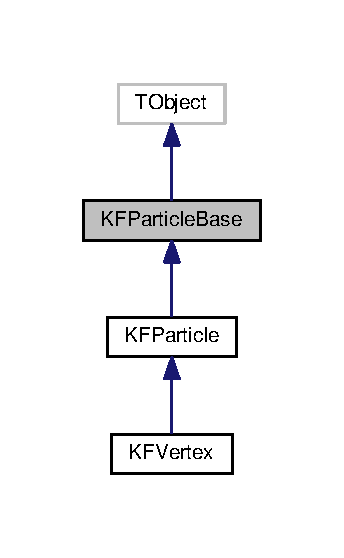
\includegraphics[width=165pt]{classKFParticleBase__inherit__graph}
\end{center}
\end{figure}


Collaboration diagram for K\+F\+Particle\+Base\+:
\nopagebreak
\begin{figure}[H]
\begin{center}
\leavevmode
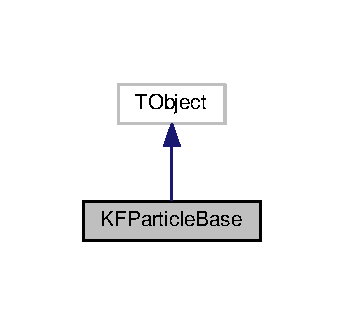
\includegraphics[width=165pt]{classKFParticleBase__coll__graph}
\end{center}
\end{figure}
\subsection*{Public Member Functions}
\begin{DoxyCompactItemize}
\item 
virtual void \hyperlink{classKFParticleBase_a54fa32dca24a267d19ac11875a650f96}{Get\+Field\+Value} (const float xyz\mbox{[}$\,$\mbox{]}, float B\mbox{[}$\,$\mbox{]}) const =0
\item 
virtual float \hyperlink{classKFParticleBase_ae4235191e7d6baaa1054507e3cb92dc9}{Get\+D\+Sto\+Point} (const float xyz\mbox{[}3\mbox{]}, float dsdr\mbox{[}6\mbox{]}) const =0
\item 
float \hyperlink{classKFParticleBase_aee9617e04925c7b26e0c9ff19c7f929e}{Get\+D\+Sto\+Point\+Line} (const float xyz\mbox{[}3\mbox{]}, float dsdr\mbox{[}6\mbox{]}) const 
\item 
float \hyperlink{classKFParticleBase_a5d8cbbe939f2be781ec24cb48f0c183f}{Get\+D\+Sto\+Point\+Bz} (float B, const float xyz\mbox{[}3\mbox{]}, float dsdr\mbox{[}6\mbox{]}, const float $\ast$param=nullptr) const 
\item 
float \hyperlink{classKFParticleBase_af9764a6d434abc765bbd3721b829f173}{Get\+D\+Sto\+Point\+By} (float By, const float xyz\mbox{[}3\mbox{]}, float dsdr\mbox{[}6\mbox{]}) const 
\item 
float \hyperlink{classKFParticleBase_a13a3715c54a4cb7b15f3f1cdfd98c8f6}{Get\+D\+Sto\+PointB} (const float $\ast$B, const float xyz\mbox{[}3\mbox{]}, float dsdr\mbox{[}6\mbox{]}) const 
\item 
float \hyperlink{classKFParticleBase_afe8330eb2ff5650fbf71c42da09cb899}{Get\+D\+Sto\+Point\+C\+BM} (const float xyz\mbox{[}3\mbox{]}, float dsdr\mbox{[}6\mbox{]}) const 
\item 
virtual void \hyperlink{classKFParticleBase_ada459a0ed2508dbc79ff582a3a32c574}{Get\+D\+Sto\+Particle} (const \hyperlink{classKFParticleBase}{K\+F\+Particle\+Base} \&p, float dS\mbox{[}2\mbox{]}, float dsdr\mbox{[}4\mbox{]}\mbox{[}6\mbox{]}) const =0
\item 
void \hyperlink{classKFParticleBase_a7d14ee08adf1bf707aa3e682f1d7b8d7}{Get\+D\+Sto\+Particle\+Line} (const \hyperlink{classKFParticleBase}{K\+F\+Particle\+Base} \&p, float dS\mbox{[}2\mbox{]}, float dsdr\mbox{[}4\mbox{]}\mbox{[}6\mbox{]}) const 
\item 
void \hyperlink{classKFParticleBase_af08e470a34c3dfd8ad208fe692a141fb}{Get\+D\+Sto\+Particle\+Bz} (float Bz, const \hyperlink{classKFParticleBase}{K\+F\+Particle\+Base} \&p, float dS\mbox{[}2\mbox{]}, float dsdr\mbox{[}4\mbox{]}\mbox{[}6\mbox{]}, const float $\ast$param1=nullptr, const float $\ast$param2=nullptr) const 
\item 
void \hyperlink{classKFParticleBase_adc56a774e8b806e9d7f0202d66d9e706}{Get\+D\+Sto\+Particle\+By} (float B, const \hyperlink{classKFParticleBase}{K\+F\+Particle\+Base} \&p, float dS\mbox{[}2\mbox{]}, float dsdr\mbox{[}4\mbox{]}\mbox{[}6\mbox{]}) const 
\item 
void \hyperlink{classKFParticleBase_a8a48edc283143f590c86a970c5df5d5c}{Get\+D\+Sto\+Particle\+C\+BM} (const \hyperlink{classKFParticleBase}{K\+F\+Particle\+Base} \&p, float dS\mbox{[}2\mbox{]}, float dsdr\mbox{[}4\mbox{]}\mbox{[}6\mbox{]}) const 
\item 
virtual void \hyperlink{classKFParticleBase_a82e0481fd804e1a2f4e87ab4d93761c9}{Transport} (float dS, const float dsdr\mbox{[}6\mbox{]}, float P\mbox{[}$\,$\mbox{]}, float C\mbox{[}$\,$\mbox{]}, float $\ast$dsdr1=nullptr, float $\ast$F=nullptr, float $\ast$F1=nullptr) const =0
\item 
virtual \hyperlink{classKFParticleBase_a53ab5233995bbc10fb2469fa4e2629e7}{$\sim$\+K\+F\+Particle\+Base} ()\hypertarget{classKFParticleBase_a53ab5233995bbc10fb2469fa4e2629e7}{}\label{classKFParticleBase_a53ab5233995bbc10fb2469fa4e2629e7}

\begin{DoxyCompactList}\small\item\em The default destructor. \end{DoxyCompactList}\item 
void \hyperlink{classKFParticleBase_a69c1005c0a85d378ca492e9140009ad1}{Initialize} (const float Param\mbox{[}$\,$\mbox{]}, const float Cov\mbox{[}$\,$\mbox{]}, Int\+\_\+t Charge, float Mass)
\item 
void \hyperlink{classKFParticleBase_a2957ab78bcb45b327959f331125e7e4a}{Initialize} ()
\item 
void \hyperlink{classKFParticleBase_a98469b9eda5343b342cfb8b2287d77bf}{Set\+Construct\+Method} (Int\+\_\+t m)\hypertarget{classKFParticleBase_a98469b9eda5343b342cfb8b2287d77bf}{}\label{classKFParticleBase_a98469b9eda5343b342cfb8b2287d77bf}

\begin{DoxyCompactList}\small\item\em Defines the construction method for the current particle (see description of f\+Construct\+Method). \end{DoxyCompactList}\item 
void \hyperlink{classKFParticleBase_a1a795bc0368ef03e7934bd8a6d4e6de4}{Set\+Mass\+Hypo} (float m)\hypertarget{classKFParticleBase_a1a795bc0368ef03e7934bd8a6d4e6de4}{}\label{classKFParticleBase_a1a795bc0368ef03e7934bd8a6d4e6de4}

\begin{DoxyCompactList}\small\item\em Sets the mass hypothesis to the particle, is used when f\+Construct\+Method = 2. \end{DoxyCompactList}\item 
const float \& \hyperlink{classKFParticleBase_a49908a949977d7311cb1eeba2c951742}{Get\+Mass\+Hypo} () const \hypertarget{classKFParticleBase_a49908a949977d7311cb1eeba2c951742}{}\label{classKFParticleBase_a49908a949977d7311cb1eeba2c951742}

\begin{DoxyCompactList}\small\item\em Returns the mass hypothesis. \end{DoxyCompactList}\item 
const float \& \hyperlink{classKFParticleBase_ad4582ede1b5ad12fdd57825458c7b316}{Get\+Sum\+Daughter\+Mass} () const \hypertarget{classKFParticleBase_ad4582ede1b5ad12fdd57825458c7b316}{}\label{classKFParticleBase_ad4582ede1b5ad12fdd57825458c7b316}

\begin{DoxyCompactList}\small\item\em Returns the sum of masses of the daughters. \end{DoxyCompactList}\item 
float \hyperlink{classKFParticleBase_afd445a88957351f077f9240a78725596}{GetX} () const \hypertarget{classKFParticleBase_afd445a88957351f077f9240a78725596}{}\label{classKFParticleBase_afd445a88957351f077f9240a78725596}

\begin{DoxyCompactList}\small\item\em Retruns X coordinate of the particle, fP\mbox{[}0\mbox{]}. \end{DoxyCompactList}\item 
float \hyperlink{classKFParticleBase_ae556c4dd7893cf3f30106488d643e724}{GetY} () const \hypertarget{classKFParticleBase_ae556c4dd7893cf3f30106488d643e724}{}\label{classKFParticleBase_ae556c4dd7893cf3f30106488d643e724}

\begin{DoxyCompactList}\small\item\em Retruns Y coordinate of the particle, fP\mbox{[}1\mbox{]}. \end{DoxyCompactList}\item 
float \hyperlink{classKFParticleBase_aa49c8625d2e60441842b7eefecfff20e}{GetZ} () const \hypertarget{classKFParticleBase_aa49c8625d2e60441842b7eefecfff20e}{}\label{classKFParticleBase_aa49c8625d2e60441842b7eefecfff20e}

\begin{DoxyCompactList}\small\item\em Retruns Z coordinate of the particle, fP\mbox{[}2\mbox{]}. \end{DoxyCompactList}\item 
float \hyperlink{classKFParticleBase_a797c4fd327ec66f1af12d947dc62fa2e}{Get\+Px} () const \hypertarget{classKFParticleBase_a797c4fd327ec66f1af12d947dc62fa2e}{}\label{classKFParticleBase_a797c4fd327ec66f1af12d947dc62fa2e}

\begin{DoxyCompactList}\small\item\em Retruns X component of the momentum, fP\mbox{[}3\mbox{]}. \end{DoxyCompactList}\item 
float \hyperlink{classKFParticleBase_aa93b12eff0960f12c0e7741129439cae}{Get\+Py} () const \hypertarget{classKFParticleBase_aa93b12eff0960f12c0e7741129439cae}{}\label{classKFParticleBase_aa93b12eff0960f12c0e7741129439cae}

\begin{DoxyCompactList}\small\item\em Retruns Y component of the momentum, fP\mbox{[}4\mbox{]}. \end{DoxyCompactList}\item 
float \hyperlink{classKFParticleBase_ae80c9269acc433d4d3fbf9041d7c3a5e}{Get\+Pz} () const \hypertarget{classKFParticleBase_ae80c9269acc433d4d3fbf9041d7c3a5e}{}\label{classKFParticleBase_ae80c9269acc433d4d3fbf9041d7c3a5e}

\begin{DoxyCompactList}\small\item\em Retruns Z component of the momentum, fP\mbox{[}5\mbox{]}. \end{DoxyCompactList}\item 
float \hyperlink{classKFParticleBase_aef14e8b7a54d4b2ed041d7d0dde5d4c4}{GetE} () const \hypertarget{classKFParticleBase_aef14e8b7a54d4b2ed041d7d0dde5d4c4}{}\label{classKFParticleBase_aef14e8b7a54d4b2ed041d7d0dde5d4c4}

\begin{DoxyCompactList}\small\item\em Returns energy of the particle, fP\mbox{[}6\mbox{]}. \end{DoxyCompactList}\item 
float \hyperlink{classKFParticleBase_a0bbf5922ff06f290eeb21065016a0353}{GetS} () const \hypertarget{classKFParticleBase_a0bbf5922ff06f290eeb21065016a0353}{}\label{classKFParticleBase_a0bbf5922ff06f290eeb21065016a0353}

\begin{DoxyCompactList}\small\item\em Returns dS=l/p, l -\/ decay length, fP\mbox{[}7\mbox{]}, defined if production vertex is set. \end{DoxyCompactList}\item 
char \hyperlink{classKFParticleBase_a97b4d2ef119c13e0117b0367473cb153}{GetQ} () const \hypertarget{classKFParticleBase_a97b4d2ef119c13e0117b0367473cb153}{}\label{classKFParticleBase_a97b4d2ef119c13e0117b0367473cb153}

\begin{DoxyCompactList}\small\item\em Returns charge of the particle. \end{DoxyCompactList}\item 
float \hyperlink{classKFParticleBase_aef4f146c36bffafe0ac1fa9a5d48ada2}{Get\+Chi2} () const \hypertarget{classKFParticleBase_aef4f146c36bffafe0ac1fa9a5d48ada2}{}\label{classKFParticleBase_aef4f146c36bffafe0ac1fa9a5d48ada2}

\begin{DoxyCompactList}\small\item\em Returns Chi2 of the fit. \end{DoxyCompactList}\item 
Int\+\_\+t \hyperlink{classKFParticleBase_a128dbedb73783a25e76a9115ec0af9ac}{Get\+N\+DF} () const \hypertarget{classKFParticleBase_a128dbedb73783a25e76a9115ec0af9ac}{}\label{classKFParticleBase_a128dbedb73783a25e76a9115ec0af9ac}

\begin{DoxyCompactList}\small\item\em Returns number of decrease of freedom. \end{DoxyCompactList}\item 
const float \& \hyperlink{classKFParticleBase_af624ef17e57f675476a2a0e597ce2983}{X} () const \hypertarget{classKFParticleBase_af624ef17e57f675476a2a0e597ce2983}{}\label{classKFParticleBase_af624ef17e57f675476a2a0e597ce2983}

\begin{DoxyCompactList}\small\item\em Retruns X coordinate of the particle, fP\mbox{[}0\mbox{]}. \end{DoxyCompactList}\item 
const float \& \hyperlink{classKFParticleBase_ad7d7e1a209955c43efac37d6136ac406}{Y} () const \hypertarget{classKFParticleBase_ad7d7e1a209955c43efac37d6136ac406}{}\label{classKFParticleBase_ad7d7e1a209955c43efac37d6136ac406}

\begin{DoxyCompactList}\small\item\em Retruns Y coordinate of the particle, fP\mbox{[}1\mbox{]}. \end{DoxyCompactList}\item 
const float \& \hyperlink{classKFParticleBase_a96e631c939d83ff67c82701ed8255200}{Z} () const \hypertarget{classKFParticleBase_a96e631c939d83ff67c82701ed8255200}{}\label{classKFParticleBase_a96e631c939d83ff67c82701ed8255200}

\begin{DoxyCompactList}\small\item\em Retruns Z coordinate of the particle, fP\mbox{[}2\mbox{]}. \end{DoxyCompactList}\item 
const float \& \hyperlink{classKFParticleBase_af8db96ad4e18b8c37444ab5d8967ad4b}{Px} () const \hypertarget{classKFParticleBase_af8db96ad4e18b8c37444ab5d8967ad4b}{}\label{classKFParticleBase_af8db96ad4e18b8c37444ab5d8967ad4b}

\begin{DoxyCompactList}\small\item\em Retruns X component of the momentum, fP\mbox{[}3\mbox{]}. \end{DoxyCompactList}\item 
const float \& \hyperlink{classKFParticleBase_a3e909ce013348a9560c6b4f4a195f99c}{Py} () const \hypertarget{classKFParticleBase_a3e909ce013348a9560c6b4f4a195f99c}{}\label{classKFParticleBase_a3e909ce013348a9560c6b4f4a195f99c}

\begin{DoxyCompactList}\small\item\em Retruns Y component of the momentum, fP\mbox{[}4\mbox{]}. \end{DoxyCompactList}\item 
const float \& \hyperlink{classKFParticleBase_a6323524db7fc97f61d8d77c0ccc362de}{Pz} () const \hypertarget{classKFParticleBase_a6323524db7fc97f61d8d77c0ccc362de}{}\label{classKFParticleBase_a6323524db7fc97f61d8d77c0ccc362de}

\begin{DoxyCompactList}\small\item\em Retruns Z component of the momentum, fP\mbox{[}5\mbox{]}. \end{DoxyCompactList}\item 
const float \& \hyperlink{classKFParticleBase_aa2f891df3d70ddcfdb32b67915c09e4b}{E} () const \hypertarget{classKFParticleBase_aa2f891df3d70ddcfdb32b67915c09e4b}{}\label{classKFParticleBase_aa2f891df3d70ddcfdb32b67915c09e4b}

\begin{DoxyCompactList}\small\item\em Returns energy of the particle, fP\mbox{[}6\mbox{]}. \end{DoxyCompactList}\item 
const float \& \hyperlink{classKFParticleBase_af9ce6c2176599a02337b472064232841}{S} () const \hypertarget{classKFParticleBase_af9ce6c2176599a02337b472064232841}{}\label{classKFParticleBase_af9ce6c2176599a02337b472064232841}

\begin{DoxyCompactList}\small\item\em Returns dS=l/p, l -\/ decay length, fP\mbox{[}7\mbox{]}, defined if production vertex is set. \end{DoxyCompactList}\item 
const char \& \hyperlink{classKFParticleBase_ae4a7bf3ab7512c1ac0110e5c405334c9}{Q} () const \hypertarget{classKFParticleBase_ae4a7bf3ab7512c1ac0110e5c405334c9}{}\label{classKFParticleBase_ae4a7bf3ab7512c1ac0110e5c405334c9}

\begin{DoxyCompactList}\small\item\em Returns charge of the particle. \end{DoxyCompactList}\item 
const float \& \hyperlink{classKFParticleBase_a970ce088efb9242fd80f3936418cbf71}{Chi2} () const \hypertarget{classKFParticleBase_a970ce088efb9242fd80f3936418cbf71}{}\label{classKFParticleBase_a970ce088efb9242fd80f3936418cbf71}

\begin{DoxyCompactList}\small\item\em Returns Chi2 of the fit. \end{DoxyCompactList}\item 
const Int\+\_\+t \& \hyperlink{classKFParticleBase_ac64a15a8896f19ff55412e9e6be60bae}{N\+DF} () const \hypertarget{classKFParticleBase_ac64a15a8896f19ff55412e9e6be60bae}{}\label{classKFParticleBase_ac64a15a8896f19ff55412e9e6be60bae}

\begin{DoxyCompactList}\small\item\em Returns number of decrease of freedom. \end{DoxyCompactList}\item 
float \hyperlink{classKFParticleBase_a73a492eea1644b514e874bbe77543c3a}{Get\+Parameter} (Int\+\_\+t i) const \hypertarget{classKFParticleBase_a73a492eea1644b514e874bbe77543c3a}{}\label{classKFParticleBase_a73a492eea1644b514e874bbe77543c3a}

\begin{DoxyCompactList}\small\item\em Returns P\mbox{[}i\mbox{]} parameter. \end{DoxyCompactList}\item 
float \hyperlink{classKFParticleBase_aa2d4b499ceab3e14819f3fbc98655950}{Get\+Covariance} (Int\+\_\+t i) const \hypertarget{classKFParticleBase_aa2d4b499ceab3e14819f3fbc98655950}{}\label{classKFParticleBase_aa2d4b499ceab3e14819f3fbc98655950}

\begin{DoxyCompactList}\small\item\em Returns C\mbox{[}i\mbox{]} element of the covariance matrix in the lower triangular form. \end{DoxyCompactList}\item 
float \hyperlink{classKFParticleBase_a4b95958ca961afb36581235d96808a01}{Get\+Covariance} (Int\+\_\+t i, Int\+\_\+t j) const \hypertarget{classKFParticleBase_a4b95958ca961afb36581235d96808a01}{}\label{classKFParticleBase_a4b95958ca961afb36581235d96808a01}

\begin{DoxyCompactList}\small\item\em Returns C\mbox{[}i,j\mbox{]} element of the covariance matrix. \end{DoxyCompactList}\item 
Int\+\_\+t \hyperlink{classKFParticleBase_a4b3409c5572d7e7735e8cf24f257e4b5}{Get\+Momentum} (float \&p, float \&error) const 
\item 
Int\+\_\+t \hyperlink{classKFParticleBase_a009ff3d3ca24073b2d5084a875202425}{Get\+Pt} (float \&pt, float \&error) const 
\item 
Int\+\_\+t \hyperlink{classKFParticleBase_a3bb4112f2132e8b01e5c1dc832c3fc39}{Get\+Eta} (float \&eta, float \&error) const 
\item 
Int\+\_\+t \hyperlink{classKFParticleBase_a2f6850dd386670f3bb4a53760022ee6f}{Get\+Phi} (float \&phi, float \&error) const 
\item 
Int\+\_\+t \hyperlink{classKFParticleBase_a31ec53f7baf5b341159d52ea2022013d}{Get\+Mass} (float \&m, float \&error) const 
\item 
Int\+\_\+t \hyperlink{classKFParticleBase_a81aaf861a28d4059cd2063649f387b8b}{Get\+Decay\+Length} (float \&l, float \&error) const 
\item 
Int\+\_\+t \hyperlink{classKFParticleBase_a15266ac3c4e995994e58061cafa12388}{Get\+Decay\+Length\+XY} (float \&l, float \&error) const 
\item 
Int\+\_\+t \hyperlink{classKFParticleBase_abc0c970f6089f124e826a1d359de73da}{Get\+Life\+Time} (float \&ctau, float \&error) const 
\item 
Int\+\_\+t \hyperlink{classKFParticleBase_a0f5d0aea519ac9d4c4051416d15b5231}{GetR} (float \&r, float \&error) const 
\item 
float \& \hyperlink{classKFParticleBase_a77a63f041716235c0d480d4cceebe6f1}{X} ()\hypertarget{classKFParticleBase_a77a63f041716235c0d480d4cceebe6f1}{}\label{classKFParticleBase_a77a63f041716235c0d480d4cceebe6f1}

\begin{DoxyCompactList}\small\item\em Modifier of X coordinate of the particle, fP\mbox{[}0\mbox{]}. \end{DoxyCompactList}\item 
float \& \hyperlink{classKFParticleBase_a1c29a8d9e7169c0b2804f0b847b46fec}{Y} ()\hypertarget{classKFParticleBase_a1c29a8d9e7169c0b2804f0b847b46fec}{}\label{classKFParticleBase_a1c29a8d9e7169c0b2804f0b847b46fec}

\begin{DoxyCompactList}\small\item\em Modifier of Y coordinate of the particle, fP\mbox{[}1\mbox{]}. \end{DoxyCompactList}\item 
float \& \hyperlink{classKFParticleBase_a2490e97a727d18d3f1ab74b2b76a796d}{Z} ()\hypertarget{classKFParticleBase_a2490e97a727d18d3f1ab74b2b76a796d}{}\label{classKFParticleBase_a2490e97a727d18d3f1ab74b2b76a796d}

\begin{DoxyCompactList}\small\item\em Modifier of Z coordinate of the particle, fP\mbox{[}2\mbox{]}. \end{DoxyCompactList}\item 
float \& \hyperlink{classKFParticleBase_af1e53bb77cab9d0273de91753c78010d}{Px} ()\hypertarget{classKFParticleBase_af1e53bb77cab9d0273de91753c78010d}{}\label{classKFParticleBase_af1e53bb77cab9d0273de91753c78010d}

\begin{DoxyCompactList}\small\item\em Modifier of X component of the momentum, fP\mbox{[}3\mbox{]}. \end{DoxyCompactList}\item 
float \& \hyperlink{classKFParticleBase_aec8b69726b2d16361a298744da70f980}{Py} ()\hypertarget{classKFParticleBase_aec8b69726b2d16361a298744da70f980}{}\label{classKFParticleBase_aec8b69726b2d16361a298744da70f980}

\begin{DoxyCompactList}\small\item\em Modifier of Y component of the momentum, fP\mbox{[}4\mbox{]}. \end{DoxyCompactList}\item 
float \& \hyperlink{classKFParticleBase_ab5d8ea3ef595ed1bbcc997c52573d9c5}{Pz} ()\hypertarget{classKFParticleBase_ab5d8ea3ef595ed1bbcc997c52573d9c5}{}\label{classKFParticleBase_ab5d8ea3ef595ed1bbcc997c52573d9c5}

\begin{DoxyCompactList}\small\item\em Modifier of Z component of the momentum, fP\mbox{[}5\mbox{]}. \end{DoxyCompactList}\item 
float \& \hyperlink{classKFParticleBase_a6b74a8cd2c67e8616dcf220e1831eb66}{E} ()\hypertarget{classKFParticleBase_a6b74a8cd2c67e8616dcf220e1831eb66}{}\label{classKFParticleBase_a6b74a8cd2c67e8616dcf220e1831eb66}

\begin{DoxyCompactList}\small\item\em Modifier of energy of the particle, fP\mbox{[}6\mbox{]}. \end{DoxyCompactList}\item 
float \& \hyperlink{classKFParticleBase_a1fab82a64b124fadb03e56a07ca6b932}{S} ()\hypertarget{classKFParticleBase_a1fab82a64b124fadb03e56a07ca6b932}{}\label{classKFParticleBase_a1fab82a64b124fadb03e56a07ca6b932}

\begin{DoxyCompactList}\small\item\em Modifier of dS=l/p, l -\/ decay length, fP\mbox{[}7\mbox{]}, defined if production vertex is set. \end{DoxyCompactList}\item 
char \& \hyperlink{classKFParticleBase_a8342e9d9208e37623a3589be872d75ad}{Q} ()\hypertarget{classKFParticleBase_a8342e9d9208e37623a3589be872d75ad}{}\label{classKFParticleBase_a8342e9d9208e37623a3589be872d75ad}

\begin{DoxyCompactList}\small\item\em Modifier of charge of the particle. \end{DoxyCompactList}\item 
float \& \hyperlink{classKFParticleBase_ac0bc1d1239aaa0b25c68f95331963a21}{Chi2} ()\hypertarget{classKFParticleBase_ac0bc1d1239aaa0b25c68f95331963a21}{}\label{classKFParticleBase_ac0bc1d1239aaa0b25c68f95331963a21}

\begin{DoxyCompactList}\small\item\em Modifier of Chi2 of the fit. \end{DoxyCompactList}\item 
Int\+\_\+t \& \hyperlink{classKFParticleBase_a35401dc9615a4181f437ba5e7015ff9a}{N\+DF} ()\hypertarget{classKFParticleBase_a35401dc9615a4181f437ba5e7015ff9a}{}\label{classKFParticleBase_a35401dc9615a4181f437ba5e7015ff9a}

\begin{DoxyCompactList}\small\item\em Modifier of number of decrease of freedom. \end{DoxyCompactList}\item 
float \& \hyperlink{classKFParticleBase_abc604c21e1ce236d94df866a3f8fb12e}{Parameter} (Int\+\_\+t i)\hypertarget{classKFParticleBase_abc604c21e1ce236d94df866a3f8fb12e}{}\label{classKFParticleBase_abc604c21e1ce236d94df866a3f8fb12e}

\begin{DoxyCompactList}\small\item\em Modifier of P\mbox{[}i\mbox{]} parameter. \end{DoxyCompactList}\item 
float \& \hyperlink{classKFParticleBase_af4cbf91f41e9dfb36faacf7f500ceb4b}{Covariance} (Int\+\_\+t i)\hypertarget{classKFParticleBase_af4cbf91f41e9dfb36faacf7f500ceb4b}{}\label{classKFParticleBase_af4cbf91f41e9dfb36faacf7f500ceb4b}

\begin{DoxyCompactList}\small\item\em Modifier of C\mbox{[}i\mbox{]} element of the covariance matrix in the lower triangular form. \end{DoxyCompactList}\item 
float \& \hyperlink{classKFParticleBase_a44abe1d32cd0049c6ff251dda1952a6c}{Covariance} (Int\+\_\+t i, Int\+\_\+t j)\hypertarget{classKFParticleBase_a44abe1d32cd0049c6ff251dda1952a6c}{}\label{classKFParticleBase_a44abe1d32cd0049c6ff251dda1952a6c}

\begin{DoxyCompactList}\small\item\em Modifier of C\mbox{[}i,j\mbox{]} element of the covariance matrix. \end{DoxyCompactList}\item 
void \hyperlink{classKFParticleBase_a907713f54a19f44caf8873a99dc51e48}{operator+=} (const \hyperlink{classKFParticleBase}{K\+F\+Particle\+Base} \&Daughter)
\item 
void \hyperlink{classKFParticleBase_a24a5ddb6e508939d630fdbeffb5cae30}{Add\+Daughter} (const \hyperlink{classKFParticleBase}{K\+F\+Particle\+Base} \&Daughter)
\item 
void \hyperlink{classKFParticleBase_ab84556dd6a10db1f6f9c5be93bc958b2}{Subtract\+Daughter} (const \hyperlink{classKFParticleBase}{K\+F\+Particle\+Base} \&Daughter)
\item 
void \hyperlink{classKFParticleBase_afe25065680801ce33287e480ca0534e4}{Add\+Daughter\+With\+Energy\+Fit} (const \hyperlink{classKFParticleBase}{K\+F\+Particle\+Base} \&Daughter)
\item 
void \hyperlink{classKFParticleBase_a143d70c6bd591a3294c4c0f89c8edcda}{Add\+Daughter\+With\+Energy\+Fit\+MC} (const \hyperlink{classKFParticleBase}{K\+F\+Particle\+Base} \&Daughter)
\item 
void \hyperlink{classKFParticleBase_a0ed85901f073ae1c6011ed7f216644d7}{Set\+Production\+Vertex} (const \hyperlink{classKFParticleBase}{K\+F\+Particle\+Base} \&Vtx)
\item 
void \hyperlink{classKFParticleBase_ac90aba4ed098945e147f1e28bb592555}{Set\+Nonlinear\+Mass\+Constraint} (float Mass)
\item 
void \hyperlink{classKFParticleBase_ab6aedf51539e2164935c6469e6b0d374}{Set\+Mass\+Constraint} (float Mass, float Sigma\+Mass=0)
\item 
void \hyperlink{classKFParticleBase_ad0c24d81f0702a7b1f3204c8f73a8e89}{Set\+No\+Decay\+Length} ()
\item 
void \hyperlink{classKFParticleBase_abc1f77ca63ec7497a457e48edec2e3fd}{Construct} (const \hyperlink{classKFParticleBase}{K\+F\+Particle\+Base} $\ast$v\+Daughters\mbox{[}$\,$\mbox{]}, Int\+\_\+t n\+Daughters, const \hyperlink{classKFParticleBase}{K\+F\+Particle\+Base} $\ast$Prod\+Vtx=nullptr, float Mass=-\/1)
\item 
void \hyperlink{classKFParticleBase_af6de8b429c89b13c29f7f8d9f6aa24c7}{Transport\+To\+Decay\+Vertex} ()
\item 
void \hyperlink{classKFParticleBase_ab33bc7d9a1d4e8c38075c37308f5b1f6}{Transport\+To\+Production\+Vertex} ()
\item 
void \hyperlink{classKFParticleBase_a0048b51a7253c7ac3af2c3c539f57cc7}{Transport\+To\+DS} (float dS, const float $\ast$dsdr)
\item 
void \hyperlink{classKFParticleBase_a88bf4e09f3a56166783df8aea759f091}{Transport\+Bz} (float Bz, float dS, const float $\ast$dsdr, float P\mbox{[}$\,$\mbox{]}, float C\mbox{[}$\,$\mbox{]}, const float $\ast$dsdr1=nullptr, float $\ast$F=nullptr, float $\ast$F1=nullptr) const 
\item 
void \hyperlink{classKFParticleBase_a36d1291524f0ac5f03c5992d9a8423fb}{Transport\+C\+BM} (float dS, const float $\ast$dsdr, float P\mbox{[}$\,$\mbox{]}, float C\mbox{[}$\,$\mbox{]}, float $\ast$dsdr1=nullptr, float $\ast$F=0, float $\ast$F1=nullptr) const 
\item 
float \hyperlink{classKFParticleBase_a0b0b6dadfff81ec0859e8bb5a70855de}{Get\+Distance\+From\+Vertex} (const float vtx\mbox{[}$\,$\mbox{]}) const 
\item 
float \hyperlink{classKFParticleBase_afd262e70a5886304084ac211e6e0a93e}{Get\+Distance\+From\+Vertex} (const \hyperlink{classKFParticleBase}{K\+F\+Particle\+Base} \&Vtx) const 
\item 
float \hyperlink{classKFParticleBase_a4f0714900bbae86b5dcc9459c08a6bd0}{Get\+Distance\+From\+Particle} (const \hyperlink{classKFParticleBase}{K\+F\+Particle\+Base} \&p) const 
\item 
float \hyperlink{classKFParticleBase_a163498359371fb50f40fa168d221f09a}{Get\+Deviation\+From\+Vertex} (const float v\mbox{[}$\,$\mbox{]}, const float Cv\mbox{[}$\,$\mbox{]}=nullptr) const 
\item 
float \hyperlink{classKFParticleBase_af96a10f763186cc66c6a298cdc34f226}{Get\+Deviation\+From\+Vertex} (const \hyperlink{classKFParticleBase}{K\+F\+Particle\+Base} \&Vtx) const 
\item 
float \hyperlink{classKFParticleBase_a1b27163a487575680c1d0bb54e30edae}{Get\+Deviation\+From\+Particle} (const \hyperlink{classKFParticleBase}{K\+F\+Particle\+Base} \&p) const 
\item 
void \hyperlink{classKFParticleBase_a61b2ddef3be58d0a9199371ef818abec}{Subtract\+From\+Vertex} (\hyperlink{classKFParticleBase}{K\+F\+Particle\+Base} \&Vtx) const 
\item 
void \hyperlink{classKFParticleBase_a870c6ea92e96afd7ad29fc2a4114eea2}{Subtract\+From\+Particle} (\hyperlink{classKFParticleBase}{K\+F\+Particle\+Base} \&Vtx) const 
\item 
void \hyperlink{classKFParticleBase_a5157686e0eeca2064da38b2cd4f225ed}{Rotate\+XY} (float angle, const float Vtx\mbox{[}3\mbox{]})
\item 
int \hyperlink{classKFParticleBase_a625f1f975f4a106df47ec12710e82f7b}{Id} () const \hypertarget{classKFParticleBase_a625f1f975f4a106df47ec12710e82f7b}{}\label{classKFParticleBase_a625f1f975f4a106df47ec12710e82f7b}

\begin{DoxyCompactList}\small\item\em Returns Id of the particle. \end{DoxyCompactList}\item 
int \hyperlink{classKFParticleBase_a5804383f749253e8a17c594ccf463842}{N\+Daughters} () const \hypertarget{classKFParticleBase_a5804383f749253e8a17c594ccf463842}{}\label{classKFParticleBase_a5804383f749253e8a17c594ccf463842}

\begin{DoxyCompactList}\small\item\em Returns number of daughter particles. \end{DoxyCompactList}\item 
const std\+::vector$<$ int $>$ \& \hyperlink{classKFParticleBase_a7f6754ebbbeb73d4c2b88a49b75db474}{Daughter\+Ids} () const \hypertarget{classKFParticleBase_a7f6754ebbbeb73d4c2b88a49b75db474}{}\label{classKFParticleBase_a7f6754ebbbeb73d4c2b88a49b75db474}

\begin{DoxyCompactList}\small\item\em Returns the vector with the indices of daughter particles. \end{DoxyCompactList}\item 
void \hyperlink{classKFParticleBase_a06b53cef25f218f5eb041197455ad0b4}{Clean\+Daughters\+Id} ()\hypertarget{classKFParticleBase_a06b53cef25f218f5eb041197455ad0b4}{}\label{classKFParticleBase_a06b53cef25f218f5eb041197455ad0b4}

\begin{DoxyCompactList}\small\item\em Cleans the vector with the indices of daughter particles. \end{DoxyCompactList}\item 
void \hyperlink{classKFParticleBase_ad223c0ea998d4c27a768291b6288c0c2}{Set\+Id} (int id)\hypertarget{classKFParticleBase_ad223c0ea998d4c27a768291b6288c0c2}{}\label{classKFParticleBase_ad223c0ea998d4c27a768291b6288c0c2}

\begin{DoxyCompactList}\small\item\em Sets the Id of the particle. After the construction of a particle should be set by user. \end{DoxyCompactList}\item 
void \hyperlink{classKFParticleBase_ab29274a82822129a02a2c856e495b8ee}{Add\+Daughter\+Id} (int id)\hypertarget{classKFParticleBase_ab29274a82822129a02a2c856e495b8ee}{}\label{classKFParticleBase_ab29274a82822129a02a2c856e495b8ee}

\begin{DoxyCompactList}\small\item\em Adds index of the daughter particle. \end{DoxyCompactList}\item 
void \hyperlink{classKFParticleBase_a3acaec6e2b8d7b0e55b37233fd091555}{Set\+P\+DG} (int pdg)\hypertarget{classKFParticleBase_a3acaec6e2b8d7b0e55b37233fd091555}{}\label{classKFParticleBase_a3acaec6e2b8d7b0e55b37233fd091555}

\begin{DoxyCompactList}\small\item\em Sets the P\+DG hypothesis. \end{DoxyCompactList}\item 
int \hyperlink{classKFParticleBase_a03ddf1d1cedebfe9265f89d38cc683f7}{Get\+P\+DG} () const \hypertarget{classKFParticleBase_a03ddf1d1cedebfe9265f89d38cc683f7}{}\label{classKFParticleBase_a03ddf1d1cedebfe9265f89d38cc683f7}

\begin{DoxyCompactList}\small\item\em Returns the P\+DG hypothesis. \end{DoxyCompactList}\end{DoxyCompactItemize}
\subsection*{Static Public Member Functions}
\begin{DoxyCompactItemize}
\item 
static void \hyperlink{classKFParticleBase_a7e78b231b422f5ba25cfb6ab995ed299}{Get\+Armenteros\+Podolanski} (\hyperlink{classKFParticleBase}{K\+F\+Particle\+Base} \&positive, \hyperlink{classKFParticleBase}{K\+F\+Particle\+Base} \&negative, float Qt\+Alfa\mbox{[}2\mbox{]})
\item 
static void \hyperlink{classKFParticleBase_aa0ed9e611a76fd44e0eaac9d6f504929}{Invert\+Choletsky3} (float a\mbox{[}6\mbox{]})
\item 
static void \hyperlink{classKFParticleBase_a150d29c9d64909e4783a4b5c227a9046}{Mult\+Q\+S\+Qt} (const float \hyperlink{classKFParticleBase_ae4a7bf3ab7512c1ac0110e5c405334c9}{Q}\mbox{[}$\,$\mbox{]}, const float \hyperlink{classKFParticleBase_af9ce6c2176599a02337b472064232841}{S}\mbox{[}$\,$\mbox{]}, float S\+Out\mbox{[}$\,$\mbox{]}, int kN)
\end{DoxyCompactItemize}
\subsection*{Protected Member Functions}
\begin{DoxyCompactItemize}
\item 
float \& \hyperlink{classKFParticleBase_aeab9a3989e50d30810c3affb483254c7}{Cij} (Int\+\_\+t i, Int\+\_\+t j)
\item 
void \hyperlink{classKFParticleBase_ad6268b20f07f2ac95af35f8f53175bd7}{Transport\+Line} (float \hyperlink{classKFParticleBase_af9ce6c2176599a02337b472064232841}{S}, const float $\ast$dsdr, float P\mbox{[}$\,$\mbox{]}, float C\mbox{[}$\,$\mbox{]}, const float $\ast$dsdr1, float $\ast$F, float $\ast$F1) const 
\item 
bool \hyperlink{classKFParticleBase_a4589ae9c9872e56468d6c5dc17adcfff}{Get\+Measurement} (const \hyperlink{classKFParticleBase}{K\+F\+Particle\+Base} \&daughter, float m\mbox{[}$\,$\mbox{]}, float V\mbox{[}$\,$\mbox{]}, float D\mbox{[}3\mbox{]}\mbox{[}3\mbox{]})
\end{DoxyCompactItemize}
\subsection*{Static Protected Member Functions}
\begin{DoxyCompactItemize}
\item 
static Int\+\_\+t \hyperlink{classKFParticleBase_ad059627ac0eb3810051cea5fbfdedc77}{IJ} (Int\+\_\+t i, Int\+\_\+t j)
\item 
static void \hyperlink{classKFParticleBase_a5baddbdf1ec37043117de66c5ab31971}{Set\+Mass\+Constraint} (float $\ast$mP, float $\ast$mC, float mJ\mbox{[}7\mbox{]}\mbox{[}7\mbox{]}, float mass)
\end{DoxyCompactItemize}
\subsection*{Protected Attributes}
\begin{DoxyCompactItemize}
\item 
float \hyperlink{classKFParticleBase_a48e6bfc3b4faad54849cf2390d88f0c2}{fP} \mbox{[}8\mbox{]}\hypertarget{classKFParticleBase_a48e6bfc3b4faad54849cf2390d88f0c2}{}\label{classKFParticleBase_a48e6bfc3b4faad54849cf2390d88f0c2}

\begin{DoxyCompactList}\small\item\em Particle parameters \{ X, Y, Z, Px, Py, Pz, E, S\mbox{[}=Decay\+Length/P\mbox{]}\}. \end{DoxyCompactList}\item 
float \hyperlink{classKFParticleBase_ab360c40ba1445910057f9ad7f2d91dbf}{fC} \mbox{[}36\mbox{]}\hypertarget{classKFParticleBase_ab360c40ba1445910057f9ad7f2d91dbf}{}\label{classKFParticleBase_ab360c40ba1445910057f9ad7f2d91dbf}

\begin{DoxyCompactList}\small\item\em Low-\/triangle covariance matrix of fP. \end{DoxyCompactList}\item 
float \hyperlink{classKFParticleBase_a357092c0e3b9098e3ec7b214c6ed8002}{f\+Chi2}\hypertarget{classKFParticleBase_a357092c0e3b9098e3ec7b214c6ed8002}{}\label{classKFParticleBase_a357092c0e3b9098e3ec7b214c6ed8002}

\begin{DoxyCompactList}\small\item\em Chi$^\wedge$2. \end{DoxyCompactList}\item 
float \hyperlink{classKFParticleBase_a74aaf87923566638d5e80f6dec9593f9}{f\+S\+From\+Decay}\hypertarget{classKFParticleBase_a74aaf87923566638d5e80f6dec9593f9}{}\label{classKFParticleBase_a74aaf87923566638d5e80f6dec9593f9}

\begin{DoxyCompactList}\small\item\em Distance from the decay vertex to the current position. \end{DoxyCompactList}\item 
float \hyperlink{classKFParticleBase_aec9dca48a7a7160607cd6198a692c46d}{Sum\+Daughter\+Mass}\hypertarget{classKFParticleBase_aec9dca48a7a7160607cd6198a692c46d}{}\label{classKFParticleBase_aec9dca48a7a7160607cd6198a692c46d}

\begin{DoxyCompactList}\small\item\em Sum of the daughter particles masses. Needed to set the constraint on the minimum mass during particle construction. \end{DoxyCompactList}\item 
float \hyperlink{classKFParticleBase_a36fd93a21d2d16ac791d5e1ba767ee38}{f\+Mass\+Hypo}\hypertarget{classKFParticleBase_a36fd93a21d2d16ac791d5e1ba767ee38}{}\label{classKFParticleBase_a36fd93a21d2d16ac791d5e1ba767ee38}

\begin{DoxyCompactList}\small\item\em The mass hypothesis, used for the constraints during particle construction. \end{DoxyCompactList}\item 
Int\+\_\+t \hyperlink{classKFParticleBase_aeb5e1343407d7e851b9087133bf42732}{f\+N\+DF}\hypertarget{classKFParticleBase_aeb5e1343407d7e851b9087133bf42732}{}\label{classKFParticleBase_aeb5e1343407d7e851b9087133bf42732}

\begin{DoxyCompactList}\small\item\em Number of degrees of freedom. \end{DoxyCompactList}\item 
int \hyperlink{classKFParticleBase_a14cbc0e0366410bda673a2eeedddecf3}{f\+Id}\hypertarget{classKFParticleBase_a14cbc0e0366410bda673a2eeedddecf3}{}\label{classKFParticleBase_a14cbc0e0366410bda673a2eeedddecf3}

\begin{DoxyCompactList}\small\item\em Id of the particle. \end{DoxyCompactList}\item 
Bool\+\_\+t \hyperlink{classKFParticleBase_a6577f7c0a81c362bb19bdefa2bd89908}{f\+At\+Production\+Vertex}\hypertarget{classKFParticleBase_a6577f7c0a81c362bb19bdefa2bd89908}{}\label{classKFParticleBase_a6577f7c0a81c362bb19bdefa2bd89908}

\begin{DoxyCompactList}\small\item\em Flag shows if particle is at the production point. \end{DoxyCompactList}\item 
char \hyperlink{classKFParticleBase_a2668110f8c75522e1cfc51496652435e}{fQ}\hypertarget{classKFParticleBase_a2668110f8c75522e1cfc51496652435e}{}\label{classKFParticleBase_a2668110f8c75522e1cfc51496652435e}

\begin{DoxyCompactList}\small\item\em The charge of the particle in the units of the elementary charge. \end{DoxyCompactList}\item 
char \hyperlink{classKFParticleBase_a6cc71ce0845697b3427db70690a509d9}{f\+Construct\+Method}\hypertarget{classKFParticleBase_a6cc71ce0845697b3427db70690a509d9}{}\label{classKFParticleBase_a6cc71ce0845697b3427db70690a509d9}

\begin{DoxyCompactList}\small\item\em Determines the method for the particle construction. ~\newline
0 -\/ Energy considered as an independent veriable, fitted independently from momentum, without any constraints on mass ~\newline
2 -\/ Energy considered as an independent variable, fitted independently from momentum, with constraints on mass of daughter particle. \end{DoxyCompactList}\item 
int \hyperlink{classKFParticleBase_ae5627ec0a06abfd66387caa7b349c0a4}{f\+P\+DG}\hypertarget{classKFParticleBase_ae5627ec0a06abfd66387caa7b349c0a4}{}\label{classKFParticleBase_ae5627ec0a06abfd66387caa7b349c0a4}

\begin{DoxyCompactList}\small\item\em The P\+DG hypothesis assigned to the particle. \end{DoxyCompactList}\item 
std\+::vector$<$ int $>$ \hyperlink{classKFParticleBase_aa6a792e88545404d791796ba32fa1515}{f\+Daughters\+Ids}\hypertarget{classKFParticleBase_aa6a792e88545404d791796ba32fa1515}{}\label{classKFParticleBase_aa6a792e88545404d791796ba32fa1515}

\begin{DoxyCompactList}\small\item\em A vector with ids of the daughter particles\+: ~\newline
1) if particle is created from a track -\/ the index of the track, in this case the size of the vector is always equal to one; ~\newline
2) if particle is constructed from other particles -\/ indices of these particles in the same array. \end{DoxyCompactList}\end{DoxyCompactItemize}


\subsection{Detailed Description}
The base of \hyperlink{classKFParticle}{K\+F\+Particle} class, describes particle objects. 

\begin{DoxyAuthor}{Author}
S.\+Gorbunov, I.\+Kisel, M.\+Zyzak 
\end{DoxyAuthor}
\begin{DoxyDate}{Date}
05.\+02.\+2019 
\end{DoxyDate}
\begin{DoxyVersion}{Version}
1.\+0
\end{DoxyVersion}
Contains the main mathematics of the KF Particle . Will be merged with the \hyperlink{classKFParticle}{K\+F\+Particle} class. 

\subsection{Member Function Documentation}
\index{K\+F\+Particle\+Base@{K\+F\+Particle\+Base}!Add\+Daughter@{Add\+Daughter}}
\index{Add\+Daughter@{Add\+Daughter}!K\+F\+Particle\+Base@{K\+F\+Particle\+Base}}
\subsubsection[{\texorpdfstring{Add\+Daughter(const K\+F\+Particle\+Base \&\+Daughter)}{AddDaughter(const KFParticleBase &Daughter)}}]{\setlength{\rightskip}{0pt plus 5cm}void K\+F\+Particle\+Base\+::\+Add\+Daughter (
\begin{DoxyParamCaption}
\item[{const {\bf K\+F\+Particle\+Base} \&}]{Daughter}
\end{DoxyParamCaption}
)}\hypertarget{classKFParticleBase_a24a5ddb6e508939d630fdbeffb5cae30}{}\label{classKFParticleBase_a24a5ddb6e508939d630fdbeffb5cae30}
Adds daughter to the current particle. Depending on the selected construction method uses\+: ~\newline
1) Either simplifyed fast mathematics which consideres momentum and energy as independent variables and thus ignores constraint on the fixed mass (f\+Construct\+Method = 0). In this case the mass of the daughter particle can be corrupted when the constructed vertex is added as the measurement and the mass of the output short-\/lived particle can become unphysical -\/ smaller then the threshold. Implemented in the \hyperlink{classKFParticleBase_afe25065680801ce33287e480ca0534e4}{Add\+Daughter\+With\+Energy\+Fit()} function ~\newline
2) Or slower but correct mathematics which requires that the masses of daughter particles stays fixed in the construction process (f\+Construct\+Method = 2). Implemented in the \hyperlink{classKFParticleBase_a143d70c6bd591a3294c4c0f89c8edcda}{Add\+Daughter\+With\+Energy\+Fit\+M\+C()} function. 
\begin{DoxyParams}[1]{Parameters}
\mbox{\tt in}  & {\em Daughter} & -\/ the daughter particle\\
\hline
\end{DoxyParams}
\index{K\+F\+Particle\+Base@{K\+F\+Particle\+Base}!Add\+Daughter\+With\+Energy\+Fit@{Add\+Daughter\+With\+Energy\+Fit}}
\index{Add\+Daughter\+With\+Energy\+Fit@{Add\+Daughter\+With\+Energy\+Fit}!K\+F\+Particle\+Base@{K\+F\+Particle\+Base}}
\subsubsection[{\texorpdfstring{Add\+Daughter\+With\+Energy\+Fit(const K\+F\+Particle\+Base \&\+Daughter)}{AddDaughterWithEnergyFit(const KFParticleBase &Daughter)}}]{\setlength{\rightskip}{0pt plus 5cm}void K\+F\+Particle\+Base\+::\+Add\+Daughter\+With\+Energy\+Fit (
\begin{DoxyParamCaption}
\item[{const {\bf K\+F\+Particle\+Base} \&}]{Daughter}
\end{DoxyParamCaption}
)}\hypertarget{classKFParticleBase_afe25065680801ce33287e480ca0534e4}{}\label{classKFParticleBase_afe25065680801ce33287e480ca0534e4}
Adds daughter to the current particle. Uses simplifyed fast mathematics which consideres momentum and energy as independent variables and thus ignores constraint on the fixed mass. In this case the mass of the daughter particle can be corrupted when the constructed vertex is added as the measurement and the mass of the output short-\/lived particle can become unphysical -\/ smaller then the threshold. 
\begin{DoxyParams}[1]{Parameters}
\mbox{\tt in}  & {\em Daughter} & -\/ the daughter particle\\
\hline
\end{DoxyParams}
\index{K\+F\+Particle\+Base@{K\+F\+Particle\+Base}!Add\+Daughter\+With\+Energy\+Fit\+MC@{Add\+Daughter\+With\+Energy\+Fit\+MC}}
\index{Add\+Daughter\+With\+Energy\+Fit\+MC@{Add\+Daughter\+With\+Energy\+Fit\+MC}!K\+F\+Particle\+Base@{K\+F\+Particle\+Base}}
\subsubsection[{\texorpdfstring{Add\+Daughter\+With\+Energy\+Fit\+M\+C(const K\+F\+Particle\+Base \&\+Daughter)}{AddDaughterWithEnergyFitMC(const KFParticleBase &Daughter)}}]{\setlength{\rightskip}{0pt plus 5cm}void K\+F\+Particle\+Base\+::\+Add\+Daughter\+With\+Energy\+Fit\+MC (
\begin{DoxyParamCaption}
\item[{const {\bf K\+F\+Particle\+Base} \&}]{Daughter}
\end{DoxyParamCaption}
)}\hypertarget{classKFParticleBase_a143d70c6bd591a3294c4c0f89c8edcda}{}\label{classKFParticleBase_a143d70c6bd591a3294c4c0f89c8edcda}
Adds daughter to the current particle. Uses slower but correct mathematics which requires that the masses of daughter particles stays fixed in the construction process. 
\begin{DoxyParams}[1]{Parameters}
\mbox{\tt in}  & {\em Daughter} & -\/ the daughter particle\\
\hline
\end{DoxyParams}
\index{K\+F\+Particle\+Base@{K\+F\+Particle\+Base}!Cij@{Cij}}
\index{Cij@{Cij}!K\+F\+Particle\+Base@{K\+F\+Particle\+Base}}
\subsubsection[{\texorpdfstring{Cij(\+Int\+\_\+t i, Int\+\_\+t j)}{Cij(Int_t i, Int_t j)}}]{\setlength{\rightskip}{0pt plus 5cm}float\& K\+F\+Particle\+Base\+::\+Cij (
\begin{DoxyParamCaption}
\item[{Int\+\_\+t}]{i, }
\item[{Int\+\_\+t}]{j}
\end{DoxyParamCaption}
)\hspace{0.3cm}{\ttfamily [inline]}, {\ttfamily [protected]}}\hypertarget{classKFParticleBase_aeab9a3989e50d30810c3affb483254c7}{}\label{classKFParticleBase_aeab9a3989e50d30810c3affb483254c7}
Return an element of the covariance matrix with \{i,j\} indices. \index{K\+F\+Particle\+Base@{K\+F\+Particle\+Base}!Construct@{Construct}}
\index{Construct@{Construct}!K\+F\+Particle\+Base@{K\+F\+Particle\+Base}}
\subsubsection[{\texorpdfstring{Construct(const K\+F\+Particle\+Base $\ast$v\+Daughters[], Int\+\_\+t n\+Daughters, const K\+F\+Particle\+Base $\ast$\+Prod\+Vtx=nullptr, float Mass=-\/1)}{Construct(const KFParticleBase *vDaughters[], Int_t nDaughters, const KFParticleBase *ProdVtx=nullptr, float Mass=-1)}}]{\setlength{\rightskip}{0pt plus 5cm}void K\+F\+Particle\+Base\+::\+Construct (
\begin{DoxyParamCaption}
\item[{const {\bf K\+F\+Particle\+Base} $\ast$}]{v\+Daughters\mbox{[}$\,$\mbox{]}, }
\item[{Int\+\_\+t}]{n\+Daughters, }
\item[{const {\bf K\+F\+Particle\+Base} $\ast$}]{Prod\+Vtx = {\ttfamily nullptr}, }
\item[{float}]{Mass = {\ttfamily -\/1}}
\end{DoxyParamCaption}
)}\hypertarget{classKFParticleBase_abc1f77ca63ec7497a457e48edec2e3fd}{}\label{classKFParticleBase_abc1f77ca63ec7497a457e48edec2e3fd}
Constructs a short-\/lived particle from a set of daughter particles\+:~\newline
1) all parameters of the \char`\"{}this\char`\"{} objects are initialised;~\newline
2) daughters are added one after another;~\newline
3) if Parent pointer is not null, the production vertex is set to it;~\newline
4) if Mass hypothesis $>$=0 the mass constraint is set. 
\begin{DoxyParams}[1]{Parameters}
\mbox{\tt in}  & {\em v\+Daughters} & -\/ array of daughter particles \\
\hline
\mbox{\tt in}  & {\em n\+Daughters} & -\/ number of daughter particles in the input array \\
\hline
\mbox{\tt in}  & {\em Parent} & -\/ optional parrent particle \\
\hline
\mbox{\tt in}  & {\em Mass} & -\/ optional mass hypothesis\\
\hline
\end{DoxyParams}
\index{K\+F\+Particle\+Base@{K\+F\+Particle\+Base}!Get\+Armenteros\+Podolanski@{Get\+Armenteros\+Podolanski}}
\index{Get\+Armenteros\+Podolanski@{Get\+Armenteros\+Podolanski}!K\+F\+Particle\+Base@{K\+F\+Particle\+Base}}
\subsubsection[{\texorpdfstring{Get\+Armenteros\+Podolanski(\+K\+F\+Particle\+Base \&positive, K\+F\+Particle\+Base \&negative, float Qt\+Alfa[2])}{GetArmenterosPodolanski(KFParticleBase &positive, KFParticleBase &negative, float QtAlfa[2])}}]{\setlength{\rightskip}{0pt plus 5cm}void K\+F\+Particle\+Base\+::\+Get\+Armenteros\+Podolanski (
\begin{DoxyParamCaption}
\item[{{\bf K\+F\+Particle\+Base} \&}]{positive, }
\item[{{\bf K\+F\+Particle\+Base} \&}]{negative, }
\item[{float}]{Qt\+Alfa\mbox{[}2\mbox{]}}
\end{DoxyParamCaption}
)\hspace{0.3cm}{\ttfamily [static]}}\hypertarget{classKFParticleBase_a7e78b231b422f5ba25cfb6ab995ed299}{}\label{classKFParticleBase_a7e78b231b422f5ba25cfb6ab995ed299}
Calculates parameters for the Armenteros-\/\+Podolanski plot for two particles. Example how to use\+:~\newline
\hyperlink{classKFParticle}{K\+F\+Particle} Pos\+Particle(...) ~\newline
\hyperlink{classKFParticle}{K\+F\+Particle} Neg\+Particle(...) ~\newline
Gamma.\+Construct\+Gamma(\+Pos\+Particle, Neg\+Particle); ~\newline
float Vertex\+Gamma\mbox{[}3\mbox{]} = \{Gamma.\+Get\+X(), Gamma.\+Get\+Y(), Gamma.\+Get\+Z()\}; ~\newline
Pos\+Particle.\+Transport\+To\+Point(\+Vertex\+Gamma); ~\newline
Neg\+Particle.\+Transport\+To\+Point(\+Vertex\+Gamma); ~\newline
float armenteros\+Qt\+Alfa\mbox{[}2\mbox{]} = \{0.\}; ~\newline
K\+F\+Particle\+::\+Get\+Armenteros\+Podolanski(\+Pos\+Particle, Neg\+Particle, armenteros\+Qt\+Alfa ); ~\newline

\begin{DoxyParams}[1]{Parameters}
\mbox{\tt in}  & {\em positive} & -\/ first particle, positive or neutral \\
\hline
\mbox{\tt in}  & {\em negative} & -\/ second particle, negative or neutral \\
\hline
\mbox{\tt out}  & {\em Qt\+Alfa\mbox{[}2\mbox{]}} & -\/ parameters for the Armenteros-\/\+Podolanski plot\+: Qt\+Alfa\mbox{[}0\mbox{]} = qt -\/ projection of the momenta of the particles on the transverse direction with respect to the total momentum, same for both particles; Qt\+Alfa\mbox{[}1\mbox{]} = (Pl+ -\/ Pl-\/)/(Pl+ + Pl-\/) -\/ combination of the longitudinal components.\\
\hline
\end{DoxyParams}
\index{K\+F\+Particle\+Base@{K\+F\+Particle\+Base}!Get\+Decay\+Length@{Get\+Decay\+Length}}
\index{Get\+Decay\+Length@{Get\+Decay\+Length}!K\+F\+Particle\+Base@{K\+F\+Particle\+Base}}
\subsubsection[{\texorpdfstring{Get\+Decay\+Length(float \&l, float \&error) const }{GetDecayLength(float &l, float &error) const }}]{\setlength{\rightskip}{0pt plus 5cm}Int\+\_\+t K\+F\+Particle\+Base\+::\+Get\+Decay\+Length (
\begin{DoxyParamCaption}
\item[{float \&}]{l, }
\item[{float \&}]{error}
\end{DoxyParamCaption}
) const}\hypertarget{classKFParticleBase_a81aaf861a28d4059cd2063649f387b8b}{}\label{classKFParticleBase_a81aaf861a28d4059cd2063649f387b8b}
Calculates the decay length of the particle in the laboratory system and its error. If they are well defined returns 0, otherwise 1. The production point should be set before calling this function. 
\begin{DoxyParams}[1]{Parameters}
\mbox{\tt out}  & {\em l} & -\/ the decay length \\
\hline
\mbox{\tt out}  & {\em error} & -\/ its error\\
\hline
\end{DoxyParams}
\index{K\+F\+Particle\+Base@{K\+F\+Particle\+Base}!Get\+Decay\+Length\+XY@{Get\+Decay\+Length\+XY}}
\index{Get\+Decay\+Length\+XY@{Get\+Decay\+Length\+XY}!K\+F\+Particle\+Base@{K\+F\+Particle\+Base}}
\subsubsection[{\texorpdfstring{Get\+Decay\+Length\+X\+Y(float \&l, float \&error) const }{GetDecayLengthXY(float &l, float &error) const }}]{\setlength{\rightskip}{0pt plus 5cm}Int\+\_\+t K\+F\+Particle\+Base\+::\+Get\+Decay\+Length\+XY (
\begin{DoxyParamCaption}
\item[{float \&}]{l, }
\item[{float \&}]{error}
\end{DoxyParamCaption}
) const}\hypertarget{classKFParticleBase_a15266ac3c4e995994e58061cafa12388}{}\label{classKFParticleBase_a15266ac3c4e995994e58061cafa12388}
Calculates the projection in the XY plane of the decay length of the particle in the laboratory system and its error. If they are well defined returns 0, otherwise 1. The production point should be set before calling this function. 
\begin{DoxyParams}[1]{Parameters}
\mbox{\tt out}  & {\em l} & -\/ the decay length \\
\hline
\mbox{\tt out}  & {\em error} & -\/ its error\\
\hline
\end{DoxyParams}
\index{K\+F\+Particle\+Base@{K\+F\+Particle\+Base}!Get\+Deviation\+From\+Particle@{Get\+Deviation\+From\+Particle}}
\index{Get\+Deviation\+From\+Particle@{Get\+Deviation\+From\+Particle}!K\+F\+Particle\+Base@{K\+F\+Particle\+Base}}
\subsubsection[{\texorpdfstring{Get\+Deviation\+From\+Particle(const K\+F\+Particle\+Base \&p) const }{GetDeviationFromParticle(const KFParticleBase &p) const }}]{\setlength{\rightskip}{0pt plus 5cm}float K\+F\+Particle\+Base\+::\+Get\+Deviation\+From\+Particle (
\begin{DoxyParamCaption}
\item[{const {\bf K\+F\+Particle\+Base} \&}]{p}
\end{DoxyParamCaption}
) const}\hypertarget{classKFParticleBase_a1b27163a487575680c1d0bb54e30edae}{}\label{classKFParticleBase_a1b27163a487575680c1d0bb54e30edae}
Returns Chi2 deviation of the current particle from another particle in 3D. 
\begin{DoxyParams}[1]{Parameters}
\mbox{\tt in}  & {\em p} & -\/ the second particle\\
\hline
\end{DoxyParams}
\index{K\+F\+Particle\+Base@{K\+F\+Particle\+Base}!Get\+Deviation\+From\+Vertex@{Get\+Deviation\+From\+Vertex}}
\index{Get\+Deviation\+From\+Vertex@{Get\+Deviation\+From\+Vertex}!K\+F\+Particle\+Base@{K\+F\+Particle\+Base}}
\subsubsection[{\texorpdfstring{Get\+Deviation\+From\+Vertex(const float v[], const float Cv[]=nullptr) const }{GetDeviationFromVertex(const float v[], const float Cv[]=nullptr) const }}]{\setlength{\rightskip}{0pt plus 5cm}float K\+F\+Particle\+Base\+::\+Get\+Deviation\+From\+Vertex (
\begin{DoxyParamCaption}
\item[{const float}]{v\mbox{[}$\,$\mbox{]}, }
\item[{const float}]{Cv\mbox{[}$\,$\mbox{]} = {\ttfamily nullptr}}
\end{DoxyParamCaption}
) const}\hypertarget{classKFParticleBase_a163498359371fb50f40fa168d221f09a}{}\label{classKFParticleBase_a163498359371fb50f40fa168d221f09a}
Returns Chi2 deviation of the current particle from the vertex v with the covariance matrix Cv in 3D. 
\begin{DoxyParams}[1]{Parameters}
\mbox{\tt in}  & {\em v\mbox{[}3\mbox{]}} & -\/ coordinates of the vertex \{X, Y, Z\} \\
\hline
\mbox{\tt in}  & {\em Cv\mbox{[}6\mbox{]}} & -\/ covariance matrix of the vertex \{Cxx, Cxy, Cyy, Cxz, Czy, Czz\}\\
\hline
\end{DoxyParams}
\index{K\+F\+Particle\+Base@{K\+F\+Particle\+Base}!Get\+Deviation\+From\+Vertex@{Get\+Deviation\+From\+Vertex}}
\index{Get\+Deviation\+From\+Vertex@{Get\+Deviation\+From\+Vertex}!K\+F\+Particle\+Base@{K\+F\+Particle\+Base}}
\subsubsection[{\texorpdfstring{Get\+Deviation\+From\+Vertex(const K\+F\+Particle\+Base \&\+Vtx) const }{GetDeviationFromVertex(const KFParticleBase &Vtx) const }}]{\setlength{\rightskip}{0pt plus 5cm}float K\+F\+Particle\+Base\+::\+Get\+Deviation\+From\+Vertex (
\begin{DoxyParamCaption}
\item[{const {\bf K\+F\+Particle\+Base} \&}]{Vtx}
\end{DoxyParamCaption}
) const}\hypertarget{classKFParticleBase_af96a10f763186cc66c6a298cdc34f226}{}\label{classKFParticleBase_af96a10f763186cc66c6a298cdc34f226}
Returns Chi2 deviation of the current particle from the vertex in the \hyperlink{classKFParticle}{K\+F\+Particle} format in 3D. 
\begin{DoxyParams}[1]{Parameters}
\mbox{\tt in}  & {\em Vtx} & -\/ the vertex in K\+F\+Partcile format\\
\hline
\end{DoxyParams}
\index{K\+F\+Particle\+Base@{K\+F\+Particle\+Base}!Get\+Distance\+From\+Particle@{Get\+Distance\+From\+Particle}}
\index{Get\+Distance\+From\+Particle@{Get\+Distance\+From\+Particle}!K\+F\+Particle\+Base@{K\+F\+Particle\+Base}}
\subsubsection[{\texorpdfstring{Get\+Distance\+From\+Particle(const K\+F\+Particle\+Base \&p) const }{GetDistanceFromParticle(const KFParticleBase &p) const }}]{\setlength{\rightskip}{0pt plus 5cm}float K\+F\+Particle\+Base\+::\+Get\+Distance\+From\+Particle (
\begin{DoxyParamCaption}
\item[{const {\bf K\+F\+Particle\+Base} \&}]{p}
\end{DoxyParamCaption}
) const}\hypertarget{classKFParticleBase_a4f0714900bbae86b5dcc9459c08a6bd0}{}\label{classKFParticleBase_a4f0714900bbae86b5dcc9459c08a6bd0}
Returns the D\+CA distance from another particle p. 
\begin{DoxyParams}[1]{Parameters}
\mbox{\tt in}  & {\em p} & -\/ the second particle\\
\hline
\end{DoxyParams}
\index{K\+F\+Particle\+Base@{K\+F\+Particle\+Base}!Get\+Distance\+From\+Vertex@{Get\+Distance\+From\+Vertex}}
\index{Get\+Distance\+From\+Vertex@{Get\+Distance\+From\+Vertex}!K\+F\+Particle\+Base@{K\+F\+Particle\+Base}}
\subsubsection[{\texorpdfstring{Get\+Distance\+From\+Vertex(const float vtx[]) const }{GetDistanceFromVertex(const float vtx[]) const }}]{\setlength{\rightskip}{0pt plus 5cm}float K\+F\+Particle\+Base\+::\+Get\+Distance\+From\+Vertex (
\begin{DoxyParamCaption}
\item[{const float}]{vtx\mbox{[}$\,$\mbox{]}}
\end{DoxyParamCaption}
) const}\hypertarget{classKFParticleBase_a0b0b6dadfff81ec0859e8bb5a70855de}{}\label{classKFParticleBase_a0b0b6dadfff81ec0859e8bb5a70855de}
Returns the D\+CA distance from vertex in 3D. 
\begin{DoxyParams}[1]{Parameters}
\mbox{\tt in}  & {\em vtx\mbox{[}3\mbox{]}} & -\/ the vertex coordinates \{X, Y, Z\}\\
\hline
\end{DoxyParams}
\index{K\+F\+Particle\+Base@{K\+F\+Particle\+Base}!Get\+Distance\+From\+Vertex@{Get\+Distance\+From\+Vertex}}
\index{Get\+Distance\+From\+Vertex@{Get\+Distance\+From\+Vertex}!K\+F\+Particle\+Base@{K\+F\+Particle\+Base}}
\subsubsection[{\texorpdfstring{Get\+Distance\+From\+Vertex(const K\+F\+Particle\+Base \&\+Vtx) const }{GetDistanceFromVertex(const KFParticleBase &Vtx) const }}]{\setlength{\rightskip}{0pt plus 5cm}float K\+F\+Particle\+Base\+::\+Get\+Distance\+From\+Vertex (
\begin{DoxyParamCaption}
\item[{const {\bf K\+F\+Particle\+Base} \&}]{Vtx}
\end{DoxyParamCaption}
) const}\hypertarget{classKFParticleBase_afd262e70a5886304084ac211e6e0a93e}{}\label{classKFParticleBase_afd262e70a5886304084ac211e6e0a93e}
Returns the D\+CA distance from vertex in the \hyperlink{classKFParticle}{K\+F\+Particle} format in 3D. 
\begin{DoxyParams}[1]{Parameters}
\mbox{\tt in}  & {\em Vtx} & -\/ the vertex in the \hyperlink{classKFParticle}{K\+F\+Particle} format\\
\hline
\end{DoxyParams}
\index{K\+F\+Particle\+Base@{K\+F\+Particle\+Base}!Get\+D\+Sto\+Particle@{Get\+D\+Sto\+Particle}}
\index{Get\+D\+Sto\+Particle@{Get\+D\+Sto\+Particle}!K\+F\+Particle\+Base@{K\+F\+Particle\+Base}}
\subsubsection[{\texorpdfstring{Get\+D\+Sto\+Particle(const K\+F\+Particle\+Base \&p, float dS[2], float dsdr[4][6]) const =0}{GetDStoParticle(const KFParticleBase &p, float dS[2], float dsdr[4][6]) const =0}}]{\setlength{\rightskip}{0pt plus 5cm}virtual void K\+F\+Particle\+Base\+::\+Get\+D\+Sto\+Particle (
\begin{DoxyParamCaption}
\item[{const {\bf K\+F\+Particle\+Base} \&}]{p, }
\item[{float}]{dS\mbox{[}2\mbox{]}, }
\item[{float}]{dsdr\mbox{[}4\mbox{]}\mbox{[}6\mbox{]}}
\end{DoxyParamCaption}
) const\hspace{0.3cm}{\ttfamily [pure virtual]}}\hypertarget{classKFParticleBase_ada459a0ed2508dbc79ff582a3a32c574}{}\label{classKFParticleBase_ada459a0ed2508dbc79ff582a3a32c574}
Virtual method to get extrapolation parameter dS=l/p to another particle. Is defined in \hyperlink{classKFParticle}{K\+F\+Particle}. 

Implemented in \hyperlink{classKFParticle_a1dfa2f6c4ec75c76a1b2aae35c05cae7}{K\+F\+Particle}.

\index{K\+F\+Particle\+Base@{K\+F\+Particle\+Base}!Get\+D\+Sto\+Particle\+By@{Get\+D\+Sto\+Particle\+By}}
\index{Get\+D\+Sto\+Particle\+By@{Get\+D\+Sto\+Particle\+By}!K\+F\+Particle\+Base@{K\+F\+Particle\+Base}}
\subsubsection[{\texorpdfstring{Get\+D\+Sto\+Particle\+By(float B, const K\+F\+Particle\+Base \&p, float dS[2], float dsdr[4][6]) const }{GetDStoParticleBy(float B, const KFParticleBase &p, float dS[2], float dsdr[4][6]) const }}]{\setlength{\rightskip}{0pt plus 5cm}void K\+F\+Particle\+Base\+::\+Get\+D\+Sto\+Particle\+By (
\begin{DoxyParamCaption}
\item[{float}]{B, }
\item[{const {\bf K\+F\+Particle\+Base} \&}]{p, }
\item[{float}]{dS\mbox{[}2\mbox{]}, }
\item[{float}]{dsdr\mbox{[}4\mbox{]}\mbox{[}6\mbox{]}}
\end{DoxyParamCaption}
) const}\hypertarget{classKFParticleBase_adc56a774e8b806e9d7f0202d66d9e706}{}\label{classKFParticleBase_adc56a774e8b806e9d7f0202d66d9e706}
Calculates dS = l/p parameters for two particles, where ~\newline
1) l -\/ signed distance to the D\+CA point with the other particle;~\newline
2) p -\/ momentum of the particle; ~\newline
under the assumption of the constant homogeneous field By. dS\mbox{[}0\mbox{]} is the transport parameter for the current particle, dS\mbox{[}1\mbox{]} -\/ for the particle \char`\"{}p\char`\"{}. Also calculates partial derivatives dsdr of the parameters dS\mbox{[}0\mbox{]} and dS\mbox{[}1\mbox{]} over the state vectors of the particles\+:~\newline
1) dsdr\mbox{[}0\mbox{]}\mbox{[}6\mbox{]} = d(d\+S\mbox{[}0\mbox{]})/d(param1);~\newline
2) dsdr\mbox{[}1\mbox{]}\mbox{[}6\mbox{]} = d(d\+S\mbox{[}0\mbox{]})/d(param2);~\newline
3) dsdr\mbox{[}2\mbox{]}\mbox{[}6\mbox{]} = d(d\+S\mbox{[}1\mbox{]})/d(param1);~\newline
4) dsdr\mbox{[}3\mbox{]}\mbox{[}6\mbox{]} = d(d\+S\mbox{[}1\mbox{]})/d(param2);~\newline
where param1 are parameters of the current particle fP and param2 are parameters of the second particle p.\+fP. The particle parameters are transformed to the coordinate system, where the main component of the magnetic field By is directed along the Z axis\+: x-\/$>$x, y-\/$>$-\/z, z-\/$>$y, and the function \hyperlink{classKFParticleBase_a5d8cbbe939f2be781ec24cb48f0c183f}{Get\+D\+Sto\+Point\+Bz()} is called. Derivatives dsdr are transformed back to the coordinate system of the particle. 
\begin{DoxyParams}[1]{Parameters}
\mbox{\tt in}  & {\em B} & -\/ magnetic field By \\
\hline
\mbox{\tt in}  & {\em p} & -\/ second particle \\
\hline
\mbox{\tt out}  & {\em d\+S\mbox{[}2\mbox{]}} & -\/ transport parameters dS for the current particle (dS\mbox{[}0\mbox{]}) and the second particle \char`\"{}p\char`\"{} (dS\mbox{[}1\mbox{]}) \\
\hline
\mbox{\tt out}  & {\em dsdr\mbox{[}4\mbox{]}\mbox{[}6\mbox{]}} & -\/ partial derivatives of the parameters dS\mbox{[}0\mbox{]} and dS\mbox{[}1\mbox{]} over the state vectors of the both particles\\
\hline
\end{DoxyParams}
\index{K\+F\+Particle\+Base@{K\+F\+Particle\+Base}!Get\+D\+Sto\+Particle\+Bz@{Get\+D\+Sto\+Particle\+Bz}}
\index{Get\+D\+Sto\+Particle\+Bz@{Get\+D\+Sto\+Particle\+Bz}!K\+F\+Particle\+Base@{K\+F\+Particle\+Base}}
\subsubsection[{\texorpdfstring{Get\+D\+Sto\+Particle\+Bz(float Bz, const K\+F\+Particle\+Base \&p, float dS[2], float dsdr[4][6], const float $\ast$param1=nullptr, const float $\ast$param2=nullptr) const }{GetDStoParticleBz(float Bz, const KFParticleBase &p, float dS[2], float dsdr[4][6], const float *param1=nullptr, const float *param2=nullptr) const }}]{\setlength{\rightskip}{0pt plus 5cm}void K\+F\+Particle\+Base\+::\+Get\+D\+Sto\+Particle\+Bz (
\begin{DoxyParamCaption}
\item[{float}]{Bz, }
\item[{const {\bf K\+F\+Particle\+Base} \&}]{p, }
\item[{float}]{dS\mbox{[}2\mbox{]}, }
\item[{float}]{dsdr\mbox{[}4\mbox{]}\mbox{[}6\mbox{]}, }
\item[{const float $\ast$}]{param1 = {\ttfamily nullptr}, }
\item[{const float $\ast$}]{param2 = {\ttfamily nullptr}}
\end{DoxyParamCaption}
) const}\hypertarget{classKFParticleBase_af08e470a34c3dfd8ad208fe692a141fb}{}\label{classKFParticleBase_af08e470a34c3dfd8ad208fe692a141fb}
Calculates dS = l/p parameters for two particles, where ~\newline
1) l -\/ signed distance to the D\+CA point with the other particle;~\newline
2) p -\/ momentum of the particle; ~\newline
under the assumption of the constant homogeneous field Bz. dS\mbox{[}0\mbox{]} is the transport parameter for the current particle, dS\mbox{[}1\mbox{]} -\/ for the particle \char`\"{}p\char`\"{}. Also calculates partial derivatives dsdr of the parameters dS\mbox{[}0\mbox{]} and dS\mbox{[}1\mbox{]} over the state vectors of the particles\+:~\newline
1) dsdr\mbox{[}0\mbox{]}\mbox{[}6\mbox{]} = d(d\+S\mbox{[}0\mbox{]})/d(param1);~\newline
2) dsdr\mbox{[}1\mbox{]}\mbox{[}6\mbox{]} = d(d\+S\mbox{[}0\mbox{]})/d(param2);~\newline
3) dsdr\mbox{[}2\mbox{]}\mbox{[}6\mbox{]} = d(d\+S\mbox{[}1\mbox{]})/d(param1);~\newline
4) dsdr\mbox{[}3\mbox{]}\mbox{[}6\mbox{]} = d(d\+S\mbox{[}1\mbox{]})/d(param2);~\newline
where param1 are parameters of the current particle (if the pointer is not provided it is initialised with fP) and param2 are parameters of the second particle \char`\"{}p\char`\"{} (if the pointer is not provided it is initialised with p.\+fP). Parameters param1 and param2 should be either provided both or both set to null pointers. 
\begin{DoxyParams}[1]{Parameters}
\mbox{\tt in}  & {\em Bz} & -\/ magnetic field Bz \\
\hline
\mbox{\tt in}  & {\em p} & -\/ second particle \\
\hline
\mbox{\tt out}  & {\em d\+S\mbox{[}2\mbox{]}} & -\/ transport parameters dS for the current particle (dS\mbox{[}0\mbox{]}) and the second particle \char`\"{}p\char`\"{} (dS\mbox{[}1\mbox{]}) \\
\hline
\mbox{\tt out}  & {\em dsdr\mbox{[}4\mbox{]}\mbox{[}6\mbox{]}} & -\/ partial derivatives of the parameters dS\mbox{[}0\mbox{]} and dS\mbox{[}1\mbox{]} over the state vectors of the both particles \\
\hline
\mbox{\tt in}  & {\em param1} & -\/ optional parameter, is used in case if the parameters of the current particles are rotated to other coordinate system (see \hyperlink{classKFParticleBase_adc56a774e8b806e9d7f0202d66d9e706}{Get\+D\+Sto\+Particle\+By()} function), otherwise fP are used \\
\hline
\mbox{\tt in}  & {\em param2} & -\/ optional parameter, is used in case if the parameters of the second particles are rotated to other coordinate system (see \hyperlink{classKFParticleBase_adc56a774e8b806e9d7f0202d66d9e706}{Get\+D\+Sto\+Particle\+By()} function), otherwise p.\+fP are used\\
\hline
\end{DoxyParams}
\index{K\+F\+Particle\+Base@{K\+F\+Particle\+Base}!Get\+D\+Sto\+Particle\+C\+BM@{Get\+D\+Sto\+Particle\+C\+BM}}
\index{Get\+D\+Sto\+Particle\+C\+BM@{Get\+D\+Sto\+Particle\+C\+BM}!K\+F\+Particle\+Base@{K\+F\+Particle\+Base}}
\subsubsection[{\texorpdfstring{Get\+D\+Sto\+Particle\+C\+B\+M(const K\+F\+Particle\+Base \&p, float dS[2], float dsdr[4][6]) const }{GetDStoParticleCBM(const KFParticleBase &p, float dS[2], float dsdr[4][6]) const }}]{\setlength{\rightskip}{0pt plus 5cm}void K\+F\+Particle\+Base\+::\+Get\+D\+Sto\+Particle\+C\+BM (
\begin{DoxyParamCaption}
\item[{const {\bf K\+F\+Particle\+Base} \&}]{p, }
\item[{float}]{dS\mbox{[}2\mbox{]}, }
\item[{float}]{dsdr\mbox{[}4\mbox{]}\mbox{[}6\mbox{]}}
\end{DoxyParamCaption}
) const}\hypertarget{classKFParticleBase_a8a48edc283143f590c86a970c5df5d5c}{}\label{classKFParticleBase_a8a48edc283143f590c86a970c5df5d5c}
Calculates dS = l/p parameters for two particles, where ~\newline
1) l -\/ signed distance to the D\+CA point with the other particle;~\newline
2) p -\/ momentum of the particle; ~\newline
in case of the C\+B\+M-\/like nonhomogeneous magnetic field. dS\mbox{[}0\mbox{]} is the transport parameter for the current particle, dS\mbox{[}1\mbox{]} -\/ for the particle \char`\"{}p\char`\"{}. Also calculates partial derivatives dsdr of the parameters dS\mbox{[}0\mbox{]} and dS\mbox{[}1\mbox{]} over the state vectors of the particles\+:~\newline
1) dsdr\mbox{[}0\mbox{]}\mbox{[}6\mbox{]} = d(d\+S\mbox{[}0\mbox{]})/d(param1);~\newline
2) dsdr\mbox{[}1\mbox{]}\mbox{[}6\mbox{]} = d(d\+S\mbox{[}0\mbox{]})/d(param2);~\newline
3) dsdr\mbox{[}2\mbox{]}\mbox{[}6\mbox{]} = d(d\+S\mbox{[}1\mbox{]})/d(param1);~\newline
4) dsdr\mbox{[}3\mbox{]}\mbox{[}6\mbox{]} = d(d\+S\mbox{[}1\mbox{]})/d(param2);~\newline
where param1 are parameters of the current particle fP and param2 are parameters of the second particle p.\+fP. For this the y-\/component of the magnetic field at the position of the current particle is obtained and the \hyperlink{classKFParticleBase_adc56a774e8b806e9d7f0202d66d9e706}{Get\+D\+Sto\+Particle\+By()} is called. It is assumed that particles are already close to each other and that the difference in magnetic field approximation between two particles can be neglected. If the charge of both particles is zero or if the magnetic field is zero the function \hyperlink{classKFParticleBase_a7d14ee08adf1bf707aa3e682f1d7b8d7}{Get\+D\+Sto\+Particle\+Line()} is called. 
\begin{DoxyParams}[1]{Parameters}
\mbox{\tt in}  & {\em p} & -\/ second particle \\
\hline
\mbox{\tt out}  & {\em d\+S\mbox{[}2\mbox{]}} & -\/ transport parameters dS for the current particle (dS\mbox{[}0\mbox{]}) and the second particle \char`\"{}p\char`\"{} (dS\mbox{[}1\mbox{]}) \\
\hline
\mbox{\tt out}  & {\em dsdr\mbox{[}4\mbox{]}\mbox{[}6\mbox{]}} & -\/ partial derivatives of the parameters dS\mbox{[}0\mbox{]} and dS\mbox{[}1\mbox{]} over the state vectors of the both particles\\
\hline
\end{DoxyParams}
\index{K\+F\+Particle\+Base@{K\+F\+Particle\+Base}!Get\+D\+Sto\+Particle\+Line@{Get\+D\+Sto\+Particle\+Line}}
\index{Get\+D\+Sto\+Particle\+Line@{Get\+D\+Sto\+Particle\+Line}!K\+F\+Particle\+Base@{K\+F\+Particle\+Base}}
\subsubsection[{\texorpdfstring{Get\+D\+Sto\+Particle\+Line(const K\+F\+Particle\+Base \&p, float dS[2], float dsdr[4][6]) const }{GetDStoParticleLine(const KFParticleBase &p, float dS[2], float dsdr[4][6]) const }}]{\setlength{\rightskip}{0pt plus 5cm}void K\+F\+Particle\+Base\+::\+Get\+D\+Sto\+Particle\+Line (
\begin{DoxyParamCaption}
\item[{const {\bf K\+F\+Particle\+Base} \&}]{p, }
\item[{float}]{dS\mbox{[}2\mbox{]}, }
\item[{float}]{dsdr\mbox{[}4\mbox{]}\mbox{[}6\mbox{]}}
\end{DoxyParamCaption}
) const}\hypertarget{classKFParticleBase_a7d14ee08adf1bf707aa3e682f1d7b8d7}{}\label{classKFParticleBase_a7d14ee08adf1bf707aa3e682f1d7b8d7}
Calculates dS = l/p parameters for two particles, where ~\newline
1) l -\/ signed distance to the D\+CA point with the other particle;~\newline
2) p -\/ momentum of the particle; ~\newline
under the assumption of the straight line trajectory. Is used for particles with charge 0 or in case of zero magnetic field. dS\mbox{[}0\mbox{]} is the transport parameter for the current particle, dS\mbox{[}1\mbox{]} -\/ for the particle \char`\"{}p\char`\"{}. Also calculates partial derivatives dsdr of the parameters dS\mbox{[}0\mbox{]} and dS\mbox{[}1\mbox{]} over the state vectors of the particles\+:~\newline
1) dsdr\mbox{[}0\mbox{]}\mbox{[}6\mbox{]} = d(d\+S\mbox{[}0\mbox{]})/d(param1);~\newline
2) dsdr\mbox{[}1\mbox{]}\mbox{[}6\mbox{]} = d(d\+S\mbox{[}0\mbox{]})/d(param2);~\newline
3) dsdr\mbox{[}2\mbox{]}\mbox{[}6\mbox{]} = d(d\+S\mbox{[}1\mbox{]})/d(param1);~\newline
4) dsdr\mbox{[}3\mbox{]}\mbox{[}6\mbox{]} = d(d\+S\mbox{[}1\mbox{]})/d(param2);~\newline
where param1 are parameters of the current particle fP and param2 are parameters of the second particle p.\+fP. 
\begin{DoxyParams}[1]{Parameters}
\mbox{\tt in}  & {\em p} & -\/ second particle \\
\hline
\mbox{\tt out}  & {\em d\+S\mbox{[}2\mbox{]}} & -\/ transport parameters dS for the current particle (dS\mbox{[}0\mbox{]}) and the second particle \char`\"{}p\char`\"{} (dS\mbox{[}1\mbox{]}) \\
\hline
\mbox{\tt out}  & {\em dsdr\mbox{[}4\mbox{]}\mbox{[}6\mbox{]}} & -\/ partial derivatives of the parameters dS\mbox{[}0\mbox{]} and dS\mbox{[}1\mbox{]} over the state vectors of the both particles\\
\hline
\end{DoxyParams}
\index{K\+F\+Particle\+Base@{K\+F\+Particle\+Base}!Get\+D\+Sto\+Point@{Get\+D\+Sto\+Point}}
\index{Get\+D\+Sto\+Point@{Get\+D\+Sto\+Point}!K\+F\+Particle\+Base@{K\+F\+Particle\+Base}}
\subsubsection[{\texorpdfstring{Get\+D\+Sto\+Point(const float xyz[3], float dsdr[6]) const =0}{GetDStoPoint(const float xyz[3], float dsdr[6]) const =0}}]{\setlength{\rightskip}{0pt plus 5cm}virtual float K\+F\+Particle\+Base\+::\+Get\+D\+Sto\+Point (
\begin{DoxyParamCaption}
\item[{const float}]{xyz\mbox{[}3\mbox{]}, }
\item[{float}]{dsdr\mbox{[}6\mbox{]}}
\end{DoxyParamCaption}
) const\hspace{0.3cm}{\ttfamily [pure virtual]}}\hypertarget{classKFParticleBase_ae4235191e7d6baaa1054507e3cb92dc9}{}\label{classKFParticleBase_ae4235191e7d6baaa1054507e3cb92dc9}
Virtual method to get extrapolation parameter dS=l/p to . Is defined in \hyperlink{classKFParticle}{K\+F\+Particle}. 

Implemented in \hyperlink{classKFParticle_af0e557256a15e60b0e3873490267b20f}{K\+F\+Particle}.

\index{K\+F\+Particle\+Base@{K\+F\+Particle\+Base}!Get\+D\+Sto\+PointB@{Get\+D\+Sto\+PointB}}
\index{Get\+D\+Sto\+PointB@{Get\+D\+Sto\+PointB}!K\+F\+Particle\+Base@{K\+F\+Particle\+Base}}
\subsubsection[{\texorpdfstring{Get\+D\+Sto\+Point\+B(const float $\ast$\+B, const float xyz[3], float dsdr[6]) const }{GetDStoPointB(const float *B, const float xyz[3], float dsdr[6]) const }}]{\setlength{\rightskip}{0pt plus 5cm}float K\+F\+Particle\+Base\+::\+Get\+D\+Sto\+PointB (
\begin{DoxyParamCaption}
\item[{const float $\ast$}]{B, }
\item[{const float}]{xyz\mbox{[}3\mbox{]}, }
\item[{float}]{dsdr\mbox{[}6\mbox{]}}
\end{DoxyParamCaption}
) const}\hypertarget{classKFParticleBase_a13a3715c54a4cb7b15f3f1cdfd98c8f6}{}\label{classKFParticleBase_a13a3715c54a4cb7b15f3f1cdfd98c8f6}
Returns dS = l/p parameter, where ~\newline
1) l -\/ signed distance to the D\+CA point with the input xyz point;~\newline
2) p -\/ momentum of the particle; ~\newline
under the assumption of the constant homogeneous field B. Also calculates partial derivatives dsdr of the parameter dS over the state vector of the current particle. The particle parameters are transformed to the coordinate system, where the magnetic field B is directed along the Z axis and the function \hyperlink{classKFParticleBase_a5d8cbbe939f2be781ec24cb48f0c183f}{Get\+D\+Sto\+Point\+Bz()} is called. Derivatives dsdr are transformed back to the coordinate system of the particle. 
\begin{DoxyParams}[1]{Parameters}
\mbox{\tt in}  & {\em B\mbox{[}3\mbox{]}} & -\/ three components of the magnetic field at the current position of the particle \\
\hline
\mbox{\tt in}  & {\em xyz\mbox{[}3\mbox{]}} & -\/ point, to which particle should be transported \\
\hline
\mbox{\tt out}  & {\em dsdr\mbox{[}6\mbox{]}} & = ds/dr -\/ partial derivatives of the parameter dS over the state vector of the current particle\\
\hline
\end{DoxyParams}
\index{K\+F\+Particle\+Base@{K\+F\+Particle\+Base}!Get\+D\+Sto\+Point\+By@{Get\+D\+Sto\+Point\+By}}
\index{Get\+D\+Sto\+Point\+By@{Get\+D\+Sto\+Point\+By}!K\+F\+Particle\+Base@{K\+F\+Particle\+Base}}
\subsubsection[{\texorpdfstring{Get\+D\+Sto\+Point\+By(float By, const float xyz[3], float dsdr[6]) const }{GetDStoPointBy(float By, const float xyz[3], float dsdr[6]) const }}]{\setlength{\rightskip}{0pt plus 5cm}float K\+F\+Particle\+Base\+::\+Get\+D\+Sto\+Point\+By (
\begin{DoxyParamCaption}
\item[{float}]{By, }
\item[{const float}]{xyz\mbox{[}3\mbox{]}, }
\item[{float}]{dsdr\mbox{[}6\mbox{]}}
\end{DoxyParamCaption}
) const}\hypertarget{classKFParticleBase_af9764a6d434abc765bbd3721b829f173}{}\label{classKFParticleBase_af9764a6d434abc765bbd3721b829f173}
Returns dS = l/p parameter, where ~\newline
1) l -\/ signed distance to the D\+CA point with the input xyz point;~\newline
2) p -\/ momentum of the particle; ~\newline
under the assumption of the constant homogeneous field By. Also calculates partial derivatives dsdr of the parameter dS over the state vector of the current particle. The particle parameters are transformed to the coordinate system, where the main component of the magnetic field By is directed along the Z axis\+: x-\/$>$x, y-\/$>$-\/z, z-\/$>$y, and the function \hyperlink{classKFParticleBase_a5d8cbbe939f2be781ec24cb48f0c183f}{Get\+D\+Sto\+Point\+Bz()} is called. Derivatives dsdr are transformed back to the coordinate system of the particle. 
\begin{DoxyParams}[1]{Parameters}
\mbox{\tt in}  & {\em By} & -\/ magnetic field By \\
\hline
\mbox{\tt in}  & {\em xyz\mbox{[}3\mbox{]}} & -\/ point, to which particle should be transported \\
\hline
\mbox{\tt out}  & {\em dsdr\mbox{[}6\mbox{]}} & = ds/dr -\/ partial derivatives of the parameter dS over the state vector of the current particle\\
\hline
\end{DoxyParams}
\index{K\+F\+Particle\+Base@{K\+F\+Particle\+Base}!Get\+D\+Sto\+Point\+Bz@{Get\+D\+Sto\+Point\+Bz}}
\index{Get\+D\+Sto\+Point\+Bz@{Get\+D\+Sto\+Point\+Bz}!K\+F\+Particle\+Base@{K\+F\+Particle\+Base}}
\subsubsection[{\texorpdfstring{Get\+D\+Sto\+Point\+Bz(float B, const float xyz[3], float dsdr[6], const float $\ast$param=nullptr) const }{GetDStoPointBz(float B, const float xyz[3], float dsdr[6], const float *param=nullptr) const }}]{\setlength{\rightskip}{0pt plus 5cm}float K\+F\+Particle\+Base\+::\+Get\+D\+Sto\+Point\+Bz (
\begin{DoxyParamCaption}
\item[{float}]{B, }
\item[{const float}]{xyz\mbox{[}3\mbox{]}, }
\item[{float}]{dsdr\mbox{[}6\mbox{]}, }
\item[{const float $\ast$}]{param = {\ttfamily nullptr}}
\end{DoxyParamCaption}
) const}\hypertarget{classKFParticleBase_a5d8cbbe939f2be781ec24cb48f0c183f}{}\label{classKFParticleBase_a5d8cbbe939f2be781ec24cb48f0c183f}
Returns dS = l/p parameter, where ~\newline
1) l -\/ signed distance to the D\+CA point with the input xyz point;~\newline
2) p -\/ momentum of the particle; ~\newline
under the assumption of the constant homogeneous field Bz. Also calculates partial derivatives dsdr of the parameter dS over the state vector of the current particle. 
\begin{DoxyParams}[1]{Parameters}
\mbox{\tt in}  & {\em B} & -\/ magnetic field Bz \\
\hline
\mbox{\tt in}  & {\em xyz\mbox{[}3\mbox{]}} & -\/ point, to which particle should be transported \\
\hline
\mbox{\tt out}  & {\em dsdr\mbox{[}6\mbox{]}} & = ds/dr partial derivatives of the parameter dS over the state vector of the current particle \\
\hline
\mbox{\tt in}  & {\em param} & -\/ optional parameter, is used in case if the parameters of the particle are rotated to other coordinate system (see \hyperlink{classKFParticleBase_af9764a6d434abc765bbd3721b829f173}{Get\+D\+Sto\+Point\+By()} function), otherwise fP are used\\
\hline
\end{DoxyParams}
\index{K\+F\+Particle\+Base@{K\+F\+Particle\+Base}!Get\+D\+Sto\+Point\+C\+BM@{Get\+D\+Sto\+Point\+C\+BM}}
\index{Get\+D\+Sto\+Point\+C\+BM@{Get\+D\+Sto\+Point\+C\+BM}!K\+F\+Particle\+Base@{K\+F\+Particle\+Base}}
\subsubsection[{\texorpdfstring{Get\+D\+Sto\+Point\+C\+B\+M(const float xyz[3], float dsdr[6]) const }{GetDStoPointCBM(const float xyz[3], float dsdr[6]) const }}]{\setlength{\rightskip}{0pt plus 5cm}float K\+F\+Particle\+Base\+::\+Get\+D\+Sto\+Point\+C\+BM (
\begin{DoxyParamCaption}
\item[{const float}]{xyz\mbox{[}3\mbox{]}, }
\item[{float}]{dsdr\mbox{[}6\mbox{]}}
\end{DoxyParamCaption}
) const}\hypertarget{classKFParticleBase_afe8330eb2ff5650fbf71c42da09cb899}{}\label{classKFParticleBase_afe8330eb2ff5650fbf71c42da09cb899}
Returns dS = l/p parameter, where ~\newline
1) l -\/ signed distance to the D\+CA point with the input xyz point;~\newline
2) p -\/ momentum of the particle; ~\newline
in case of the C\+B\+M-\/like nonhomogeneous magnetic field. Also calculates partial derivatives dsdr of the parameter dS over the state vector of the current particle. For this the y-\/component of the magnetic field at the current position of the particle is obtained and the \hyperlink{classKFParticleBase_af9764a6d434abc765bbd3721b829f173}{Get\+D\+Sto\+Point\+By()} is called. 
\begin{DoxyParams}[1]{Parameters}
\mbox{\tt in}  & {\em xyz\mbox{[}3\mbox{]}} & -\/ point, to which particle should be transported \\
\hline
\mbox{\tt out}  & {\em dsdr\mbox{[}6\mbox{]}} & = ds/dr partial derivatives of the parameter dS over the state vector of the current particle\\
\hline
\end{DoxyParams}
\index{K\+F\+Particle\+Base@{K\+F\+Particle\+Base}!Get\+D\+Sto\+Point\+Line@{Get\+D\+Sto\+Point\+Line}}
\index{Get\+D\+Sto\+Point\+Line@{Get\+D\+Sto\+Point\+Line}!K\+F\+Particle\+Base@{K\+F\+Particle\+Base}}
\subsubsection[{\texorpdfstring{Get\+D\+Sto\+Point\+Line(const float xyz[3], float dsdr[6]) const }{GetDStoPointLine(const float xyz[3], float dsdr[6]) const }}]{\setlength{\rightskip}{0pt plus 5cm}float K\+F\+Particle\+Base\+::\+Get\+D\+Sto\+Point\+Line (
\begin{DoxyParamCaption}
\item[{const float}]{xyz\mbox{[}3\mbox{]}, }
\item[{float}]{dsdr\mbox{[}6\mbox{]}}
\end{DoxyParamCaption}
) const}\hypertarget{classKFParticleBase_aee9617e04925c7b26e0c9ff19c7f929e}{}\label{classKFParticleBase_aee9617e04925c7b26e0c9ff19c7f929e}
Returns dS = l/p parameter, where ~\newline
1) l -\/ signed distance to the D\+CA point with the input xyz point;~\newline
2) p -\/ momentum of the particle; ~\newline
assuming the straigth line trajectory. Is used for particles with charge 0 or in case of zero magnetic field. Also calculates partial derivatives dsdr of the parameter dS over the state vector of the current particle. 
\begin{DoxyParams}[1]{Parameters}
\mbox{\tt in}  & {\em xyz\mbox{[}3\mbox{]}} & -\/ point where particle should be transported \\
\hline
\mbox{\tt out}  & {\em dsdr\mbox{[}6\mbox{]}} & = ds/dr partial derivatives of the parameter dS over the state vector of the current particle\\
\hline
\end{DoxyParams}
\index{K\+F\+Particle\+Base@{K\+F\+Particle\+Base}!Get\+Eta@{Get\+Eta}}
\index{Get\+Eta@{Get\+Eta}!K\+F\+Particle\+Base@{K\+F\+Particle\+Base}}
\subsubsection[{\texorpdfstring{Get\+Eta(float \&eta, float \&error) const }{GetEta(float &eta, float &error) const }}]{\setlength{\rightskip}{0pt plus 5cm}Int\+\_\+t K\+F\+Particle\+Base\+::\+Get\+Eta (
\begin{DoxyParamCaption}
\item[{float \&}]{eta, }
\item[{float \&}]{error}
\end{DoxyParamCaption}
) const}\hypertarget{classKFParticleBase_a3bb4112f2132e8b01e5c1dc832c3fc39}{}\label{classKFParticleBase_a3bb4112f2132e8b01e5c1dc832c3fc39}
Calculates particle pseudorapidity and its error. If they are well defined returns 0, otherwise 1. 
\begin{DoxyParams}[1]{Parameters}
\mbox{\tt out}  & {\em eta} & -\/ pseudorapidity of the particle \\
\hline
\mbox{\tt out}  & {\em error} & -\/ its error\\
\hline
\end{DoxyParams}
\index{K\+F\+Particle\+Base@{K\+F\+Particle\+Base}!Get\+Field\+Value@{Get\+Field\+Value}}
\index{Get\+Field\+Value@{Get\+Field\+Value}!K\+F\+Particle\+Base@{K\+F\+Particle\+Base}}
\subsubsection[{\texorpdfstring{Get\+Field\+Value(const float xyz[], float B[]) const =0}{GetFieldValue(const float xyz[], float B[]) const =0}}]{\setlength{\rightskip}{0pt plus 5cm}virtual void K\+F\+Particle\+Base\+::\+Get\+Field\+Value (
\begin{DoxyParamCaption}
\item[{const float}]{xyz\mbox{[}$\,$\mbox{]}, }
\item[{float}]{B\mbox{[}$\,$\mbox{]}}
\end{DoxyParamCaption}
) const\hspace{0.3cm}{\ttfamily [pure virtual]}}\hypertarget{classKFParticleBase_a54fa32dca24a267d19ac11875a650f96}{}\label{classKFParticleBase_a54fa32dca24a267d19ac11875a650f96}
Abstract methods are defined in the \hyperlink{classKFParticle}{K\+F\+Particle} class\+Virtual method to access the magnetic field 

Implemented in \hyperlink{classKFParticle_a586922b2bf23f335bf999f50ff5d633f}{K\+F\+Particle}.

\index{K\+F\+Particle\+Base@{K\+F\+Particle\+Base}!Get\+Life\+Time@{Get\+Life\+Time}}
\index{Get\+Life\+Time@{Get\+Life\+Time}!K\+F\+Particle\+Base@{K\+F\+Particle\+Base}}
\subsubsection[{\texorpdfstring{Get\+Life\+Time(float \&ctau, float \&error) const }{GetLifeTime(float &ctau, float &error) const }}]{\setlength{\rightskip}{0pt plus 5cm}Int\+\_\+t K\+F\+Particle\+Base\+::\+Get\+Life\+Time (
\begin{DoxyParamCaption}
\item[{float \&}]{ctau, }
\item[{float \&}]{error}
\end{DoxyParamCaption}
) const}\hypertarget{classKFParticleBase_abc0c970f6089f124e826a1d359de73da}{}\label{classKFParticleBase_abc0c970f6089f124e826a1d359de73da}
Calculates the lifetime times speed of life (ctau) \mbox{[}cm\mbox{]} of the particle in the center of mass frame and its error. If they are well defined returns 0, otherwise 1. The production point should be set before calling this function. 
\begin{DoxyParams}[1]{Parameters}
\mbox{\tt out}  & {\em ctau} & -\/ lifetime of the particle \mbox{[}cm\mbox{]} \\
\hline
\mbox{\tt out}  & {\em error} & -\/ its error\\
\hline
\end{DoxyParams}
\index{K\+F\+Particle\+Base@{K\+F\+Particle\+Base}!Get\+Mass@{Get\+Mass}}
\index{Get\+Mass@{Get\+Mass}!K\+F\+Particle\+Base@{K\+F\+Particle\+Base}}
\subsubsection[{\texorpdfstring{Get\+Mass(float \&m, float \&error) const }{GetMass(float &m, float &error) const }}]{\setlength{\rightskip}{0pt plus 5cm}Int\+\_\+t K\+F\+Particle\+Base\+::\+Get\+Mass (
\begin{DoxyParamCaption}
\item[{float \&}]{m, }
\item[{float \&}]{error}
\end{DoxyParamCaption}
) const}\hypertarget{classKFParticleBase_a31ec53f7baf5b341159d52ea2022013d}{}\label{classKFParticleBase_a31ec53f7baf5b341159d52ea2022013d}
Calculates the mass of the particle and its error. If they are well defined returns 0, otherwise 1. 
\begin{DoxyParams}[1]{Parameters}
\mbox{\tt out}  & {\em m} & -\/ mass of the particle \\
\hline
\mbox{\tt out}  & {\em error} & -\/ its error\\
\hline
\end{DoxyParams}
\index{K\+F\+Particle\+Base@{K\+F\+Particle\+Base}!Get\+Measurement@{Get\+Measurement}}
\index{Get\+Measurement@{Get\+Measurement}!K\+F\+Particle\+Base@{K\+F\+Particle\+Base}}
\subsubsection[{\texorpdfstring{Get\+Measurement(const K\+F\+Particle\+Base \&daughter, float m[], float V[], float D[3][3])}{GetMeasurement(const KFParticleBase &daughter, float m[], float V[], float D[3][3])}}]{\setlength{\rightskip}{0pt plus 5cm}bool K\+F\+Particle\+Base\+::\+Get\+Measurement (
\begin{DoxyParamCaption}
\item[{const {\bf K\+F\+Particle\+Base} \&}]{daughter, }
\item[{float}]{m\mbox{[}$\,$\mbox{]}, }
\item[{float}]{V\mbox{[}$\,$\mbox{]}, }
\item[{float}]{D\mbox{[}3\mbox{]}\mbox{[}3\mbox{]}}
\end{DoxyParamCaption}
)\hspace{0.3cm}{\ttfamily [protected]}}\hypertarget{classKFParticleBase_a4589ae9c9872e56468d6c5dc17adcfff}{}\label{classKFParticleBase_a4589ae9c9872e56468d6c5dc17adcfff}
Obtains the measurements from the current particle and the daughter to be added for the Kalman filter mathematics. If these are two first daughters they are transported to the point of the closest approach, if the third or higher daughter is added it is transported to the D\+CA point of the already constructed vertex. The correlations are taken into account in the covariance matrices of both measurements, the correlation matrix of two measurements is also calculated. Parameters of the current particle are modified by this function, the daughter is not changed, its parameters are stored to the output arrays after modifications. 
\begin{DoxyParams}[1]{Parameters}
\mbox{\tt in}  & {\em daughter} & -\/ the daughter particle to be added, stays unchanged \\
\hline
\mbox{\tt out}  & {\em m\mbox{[}8\mbox{]}} & -\/ the output parameters of the daughter particle at the D\+CA point \\
\hline
\mbox{\tt out}  & {\em V\mbox{[}36\mbox{]}} & -\/ the output covariance matrix of the daughter parameters, takes into account the correlation \\
\hline
\mbox{\tt out}  & {\em D\mbox{[}3\mbox{]}\mbox{[}3\mbox{]}} & -\/ the correlation matrix between the current and daughter particles\\
\hline
\end{DoxyParams}
\index{K\+F\+Particle\+Base@{K\+F\+Particle\+Base}!Get\+Momentum@{Get\+Momentum}}
\index{Get\+Momentum@{Get\+Momentum}!K\+F\+Particle\+Base@{K\+F\+Particle\+Base}}
\subsubsection[{\texorpdfstring{Get\+Momentum(float \&p, float \&error) const }{GetMomentum(float &p, float &error) const }}]{\setlength{\rightskip}{0pt plus 5cm}Int\+\_\+t K\+F\+Particle\+Base\+::\+Get\+Momentum (
\begin{DoxyParamCaption}
\item[{float \&}]{p, }
\item[{float \&}]{error}
\end{DoxyParamCaption}
) const}\hypertarget{classKFParticleBase_a4b3409c5572d7e7735e8cf24f257e4b5}{}\label{classKFParticleBase_a4b3409c5572d7e7735e8cf24f257e4b5}
Calculates particle momentum and its error. If they are well defined returns 0, otherwise 1. 
\begin{DoxyParams}[1]{Parameters}
\mbox{\tt out}  & {\em p} & -\/ momentum of the particle \\
\hline
\mbox{\tt out}  & {\em error} & -\/ its error\\
\hline
\end{DoxyParams}
\index{K\+F\+Particle\+Base@{K\+F\+Particle\+Base}!Get\+Phi@{Get\+Phi}}
\index{Get\+Phi@{Get\+Phi}!K\+F\+Particle\+Base@{K\+F\+Particle\+Base}}
\subsubsection[{\texorpdfstring{Get\+Phi(float \&phi, float \&error) const }{GetPhi(float &phi, float &error) const }}]{\setlength{\rightskip}{0pt plus 5cm}Int\+\_\+t K\+F\+Particle\+Base\+::\+Get\+Phi (
\begin{DoxyParamCaption}
\item[{float \&}]{phi, }
\item[{float \&}]{error}
\end{DoxyParamCaption}
) const}\hypertarget{classKFParticleBase_a2f6850dd386670f3bb4a53760022ee6f}{}\label{classKFParticleBase_a2f6850dd386670f3bb4a53760022ee6f}
Calculates particle polar angle at the current point and its error. If they are well defined returns 0, otherwise 1. 
\begin{DoxyParams}[1]{Parameters}
\mbox{\tt out}  & {\em phi} & -\/ polar angle of the particle \\
\hline
\mbox{\tt out}  & {\em error} & -\/ its error\\
\hline
\end{DoxyParams}
\index{K\+F\+Particle\+Base@{K\+F\+Particle\+Base}!Get\+Pt@{Get\+Pt}}
\index{Get\+Pt@{Get\+Pt}!K\+F\+Particle\+Base@{K\+F\+Particle\+Base}}
\subsubsection[{\texorpdfstring{Get\+Pt(float \&pt, float \&error) const }{GetPt(float &pt, float &error) const }}]{\setlength{\rightskip}{0pt plus 5cm}Int\+\_\+t K\+F\+Particle\+Base\+::\+Get\+Pt (
\begin{DoxyParamCaption}
\item[{float \&}]{pt, }
\item[{float \&}]{error}
\end{DoxyParamCaption}
) const}\hypertarget{classKFParticleBase_a009ff3d3ca24073b2d5084a875202425}{}\label{classKFParticleBase_a009ff3d3ca24073b2d5084a875202425}
Calculates particle transverse momentum and its error. If they are well defined returns 0, otherwise 1. 
\begin{DoxyParams}[1]{Parameters}
\mbox{\tt out}  & {\em pt} & -\/ transverse momentum of the particle \\
\hline
\mbox{\tt out}  & {\em error} & -\/ its error\\
\hline
\end{DoxyParams}
\index{K\+F\+Particle\+Base@{K\+F\+Particle\+Base}!GetR@{GetR}}
\index{GetR@{GetR}!K\+F\+Particle\+Base@{K\+F\+Particle\+Base}}
\subsubsection[{\texorpdfstring{Get\+R(float \&r, float \&error) const }{GetR(float &r, float &error) const }}]{\setlength{\rightskip}{0pt plus 5cm}Int\+\_\+t K\+F\+Particle\+Base\+::\+GetR (
\begin{DoxyParamCaption}
\item[{float \&}]{r, }
\item[{float \&}]{error}
\end{DoxyParamCaption}
) const}\hypertarget{classKFParticleBase_a0f5d0aea519ac9d4c4051416d15b5231}{}\label{classKFParticleBase_a0f5d0aea519ac9d4c4051416d15b5231}
Calculates the distance to the point \{0,0,0\} and its error. If they are well defined returns 0, otherwise 1. 
\begin{DoxyParams}[1]{Parameters}
\mbox{\tt out}  & {\em r} & -\/ polar angle of the particle \\
\hline
\mbox{\tt out}  & {\em error} & -\/ its error\\
\hline
\end{DoxyParams}
\index{K\+F\+Particle\+Base@{K\+F\+Particle\+Base}!IJ@{IJ}}
\index{IJ@{IJ}!K\+F\+Particle\+Base@{K\+F\+Particle\+Base}}
\subsubsection[{\texorpdfstring{I\+J(\+Int\+\_\+t i, Int\+\_\+t j)}{IJ(Int_t i, Int_t j)}}]{\setlength{\rightskip}{0pt plus 5cm}static Int\+\_\+t K\+F\+Particle\+Base\+::\+IJ (
\begin{DoxyParamCaption}
\item[{Int\+\_\+t}]{i, }
\item[{Int\+\_\+t}]{j}
\end{DoxyParamCaption}
)\hspace{0.3cm}{\ttfamily [inline]}, {\ttfamily [static]}, {\ttfamily [protected]}}\hypertarget{classKFParticleBase_ad059627ac0eb3810051cea5fbfdedc77}{}\label{classKFParticleBase_ad059627ac0eb3810051cea5fbfdedc77}
Converts a pair of indices \{i,j\} of the covariance matrix to one index corresponding to the triangular form. \index{K\+F\+Particle\+Base@{K\+F\+Particle\+Base}!Initialize@{Initialize}}
\index{Initialize@{Initialize}!K\+F\+Particle\+Base@{K\+F\+Particle\+Base}}
\subsubsection[{\texorpdfstring{Initialize(const float Param[], const float Cov[], Int\+\_\+t Charge, float Mass)}{Initialize(const float Param[], const float Cov[], Int_t Charge, float Mass)}}]{\setlength{\rightskip}{0pt plus 5cm}void K\+F\+Particle\+Base\+::\+Initialize (
\begin{DoxyParamCaption}
\item[{const float}]{Param\mbox{[}$\,$\mbox{]}, }
\item[{const float}]{Cov\mbox{[}$\,$\mbox{]}, }
\item[{Int\+\_\+t}]{Charge, }
\item[{float}]{Mass}
\end{DoxyParamCaption}
)}\hypertarget{classKFParticleBase_a69c1005c0a85d378ca492e9140009ad1}{}\label{classKFParticleBase_a69c1005c0a85d378ca492e9140009ad1}
Sets the parameters of the particle\+:


\begin{DoxyParams}[1]{Parameters}
\mbox{\tt in}  & {\em Param\mbox{[}6\mbox{]}} & = \{ X, Y, Z, Px, Py, Pz \} -\/ position and momentum \\
\hline
\mbox{\tt in}  & {\em Cov\mbox{[}21\mbox{]}} & -\/ lower-\/triangular part of the covariance matrix\+:~\newline
\begin{DoxyVerb}          (  0  .  .  .  .  . )
          (  1  2  .  .  .  . )
Cov[21] = (  3  4  5  .  .  . )
          (  6  7  8  9  .  . )
          ( 10 11 12 13 14  . )
          ( 15 16 17 18 19 20 )
\end{DoxyVerb}
 \\
\hline
\mbox{\tt in}  & {\em Charge} & -\/ charge of the particle in elementary charge units \\
\hline
\mbox{\tt in}  & {\em mass} & -\/ the mass hypothesis\\
\hline
\end{DoxyParams}
\index{K\+F\+Particle\+Base@{K\+F\+Particle\+Base}!Initialize@{Initialize}}
\index{Initialize@{Initialize}!K\+F\+Particle\+Base@{K\+F\+Particle\+Base}}
\subsubsection[{\texorpdfstring{Initialize()}{Initialize()}}]{\setlength{\rightskip}{0pt plus 5cm}void K\+F\+Particle\+Base\+::\+Initialize (
\begin{DoxyParamCaption}
{}
\end{DoxyParamCaption}
)}\hypertarget{classKFParticleBase_a2957ab78bcb45b327959f331125e7e4a}{}\label{classKFParticleBase_a2957ab78bcb45b327959f331125e7e4a}
Initialises the parameters by default\+: ~\newline
1) all parameters are set to 0; ~\newline
2) all elements of the covariance matrix are set to 0 except Cxx=Cyy=Czz=100; ~\newline
3) Q = 0; ~\newline
4) chi2 is set to 0; ~\newline
5) N\+DF = -\/3, since 3 parameters should be fitted\+: X, Y, Z.\index{K\+F\+Particle\+Base@{K\+F\+Particle\+Base}!Invert\+Choletsky3@{Invert\+Choletsky3}}
\index{Invert\+Choletsky3@{Invert\+Choletsky3}!K\+F\+Particle\+Base@{K\+F\+Particle\+Base}}
\subsubsection[{\texorpdfstring{Invert\+Choletsky3(float a[6])}{InvertCholetsky3(float a[6])}}]{\setlength{\rightskip}{0pt plus 5cm}void K\+F\+Particle\+Base\+::\+Invert\+Choletsky3 (
\begin{DoxyParamCaption}
\item[{float}]{a\mbox{[}6\mbox{]}}
\end{DoxyParamCaption}
)\hspace{0.3cm}{\ttfamily [static]}}\hypertarget{classKFParticleBase_aa0ed9e611a76fd44e0eaac9d6f504929}{}\label{classKFParticleBase_aa0ed9e611a76fd44e0eaac9d6f504929}
Inverts symmetric 3x3 matrix a using modified Choletsky decomposition. The result is stored to the same matrix a. 
\begin{DoxyParams}[1]{Parameters}
\mbox{\tt in,out}  & {\em a} & -\/ 3x3 symmetric matrix\\
\hline
\end{DoxyParams}
\index{K\+F\+Particle\+Base@{K\+F\+Particle\+Base}!Mult\+Q\+S\+Qt@{Mult\+Q\+S\+Qt}}
\index{Mult\+Q\+S\+Qt@{Mult\+Q\+S\+Qt}!K\+F\+Particle\+Base@{K\+F\+Particle\+Base}}
\subsubsection[{\texorpdfstring{Mult\+Q\+S\+Qt(const float Q[], const float S[], float S\+Out[], int k\+N)}{MultQSQt(const float Q[], const float S[], float SOut[], int kN)}}]{\setlength{\rightskip}{0pt plus 5cm}void K\+F\+Particle\+Base\+::\+Mult\+Q\+S\+Qt (
\begin{DoxyParamCaption}
\item[{const float}]{Q\mbox{[}$\,$\mbox{]}, }
\item[{const float}]{S\mbox{[}$\,$\mbox{]}, }
\item[{float}]{S\+Out\mbox{[}$\,$\mbox{]}, }
\item[{int}]{kN}
\end{DoxyParamCaption}
)\hspace{0.3cm}{\ttfamily [static]}}\hypertarget{classKFParticleBase_a150d29c9d64909e4783a4b5c227a9046}{}\label{classKFParticleBase_a150d29c9d64909e4783a4b5c227a9046}
Matrix multiplication S\+Out = Q$\ast$\+S$\ast$\+Q$^\wedge$T, where Q -\/ square matrix, S -\/ symmetric matrix. 
\begin{DoxyParams}[1]{Parameters}
\mbox{\tt in}  & {\em Q} & -\/ square matrix \\
\hline
\mbox{\tt in}  & {\em S} & -\/ input symmetric matrix \\
\hline
\mbox{\tt out}  & {\em S\+Out} & -\/ output symmetric matrix \\
\hline
\mbox{\tt in}  & {\em kN} & -\/ dimensionality of the matrices\\
\hline
\end{DoxyParams}
\index{K\+F\+Particle\+Base@{K\+F\+Particle\+Base}!operator+=@{operator+=}}
\index{operator+=@{operator+=}!K\+F\+Particle\+Base@{K\+F\+Particle\+Base}}
\subsubsection[{\texorpdfstring{operator+=(const K\+F\+Particle\+Base \&\+Daughter)}{operator+=(const KFParticleBase &Daughter)}}]{\setlength{\rightskip}{0pt plus 5cm}void K\+F\+Particle\+Base\+::operator+= (
\begin{DoxyParamCaption}
\item[{const {\bf K\+F\+Particle\+Base} \&}]{Daughter}
\end{DoxyParamCaption}
)}\hypertarget{classKFParticleBase_a907713f54a19f44caf8873a99dc51e48}{}\label{classKFParticleBase_a907713f54a19f44caf8873a99dc51e48}
Operator to add daughter to the current particle. Calls \hyperlink{classKFParticleBase_a24a5ddb6e508939d630fdbeffb5cae30}{Add\+Daughter()} function. 
\begin{DoxyParams}[1]{Parameters}
\mbox{\tt in}  & {\em Daughter} & -\/ the daughter particle\\
\hline
\end{DoxyParams}
\index{K\+F\+Particle\+Base@{K\+F\+Particle\+Base}!Rotate\+XY@{Rotate\+XY}}
\index{Rotate\+XY@{Rotate\+XY}!K\+F\+Particle\+Base@{K\+F\+Particle\+Base}}
\subsubsection[{\texorpdfstring{Rotate\+X\+Y(float angle, const float Vtx[3])}{RotateXY(float angle, const float Vtx[3])}}]{\setlength{\rightskip}{0pt plus 5cm}void K\+F\+Particle\+Base\+::\+Rotate\+XY (
\begin{DoxyParamCaption}
\item[{float}]{angle, }
\item[{const float}]{Vtx\mbox{[}3\mbox{]}}
\end{DoxyParamCaption}
)}\hypertarget{classKFParticleBase_a5157686e0eeca2064da38b2cd4f225ed}{}\label{classKFParticleBase_a5157686e0eeca2064da38b2cd4f225ed}
Rotates the \hyperlink{classKFParticle}{K\+F\+Particle} object around OZ axis, OZ axis is set by the vertex position. 
\begin{DoxyParams}[1]{Parameters}
\mbox{\tt in}  & {\em angle} & -\/ angle of rotation in XY plane in \mbox{[}rad\mbox{]} \\
\hline
\mbox{\tt in}  & {\em Vtx\mbox{[}3\mbox{]}} & -\/ position of the vertex in \mbox{[}cm\mbox{]}\\
\hline
\end{DoxyParams}
\index{K\+F\+Particle\+Base@{K\+F\+Particle\+Base}!Set\+Mass\+Constraint@{Set\+Mass\+Constraint}}
\index{Set\+Mass\+Constraint@{Set\+Mass\+Constraint}!K\+F\+Particle\+Base@{K\+F\+Particle\+Base}}
\subsubsection[{\texorpdfstring{Set\+Mass\+Constraint(float Mass, float Sigma\+Mass=0)}{SetMassConstraint(float Mass, float SigmaMass=0)}}]{\setlength{\rightskip}{0pt plus 5cm}void K\+F\+Particle\+Base\+::\+Set\+Mass\+Constraint (
\begin{DoxyParamCaption}
\item[{float}]{Mass, }
\item[{float}]{Sigma\+Mass = {\ttfamily 0}}
\end{DoxyParamCaption}
)}\hypertarget{classKFParticleBase_ab6aedf51539e2164935c6469e6b0d374}{}\label{classKFParticleBase_ab6aedf51539e2164935c6469e6b0d374}
Sets linearised mass constraint on the current particle. The constraint can be set with an uncertainty. 
\begin{DoxyParams}[1]{Parameters}
\mbox{\tt in}  & {\em Mass} & -\/ the mass to be set on the state vector mP \\
\hline
\mbox{\tt in}  & {\em Sigma\+Mass} & -\/ uncertainty of the constraint\\
\hline
\end{DoxyParams}
\index{K\+F\+Particle\+Base@{K\+F\+Particle\+Base}!Set\+Mass\+Constraint@{Set\+Mass\+Constraint}}
\index{Set\+Mass\+Constraint@{Set\+Mass\+Constraint}!K\+F\+Particle\+Base@{K\+F\+Particle\+Base}}
\subsubsection[{\texorpdfstring{Set\+Mass\+Constraint(float $\ast$m\+P, float $\ast$m\+C, float mJ[7][7], float mass)}{SetMassConstraint(float *mP, float *mC, float mJ[7][7], float mass)}}]{\setlength{\rightskip}{0pt plus 5cm}void K\+F\+Particle\+Base\+::\+Set\+Mass\+Constraint (
\begin{DoxyParamCaption}
\item[{float $\ast$}]{mP, }
\item[{float $\ast$}]{mC, }
\item[{float}]{mJ\mbox{[}7\mbox{]}\mbox{[}7\mbox{]}, }
\item[{float}]{mass}
\end{DoxyParamCaption}
)\hspace{0.3cm}{\ttfamily [static]}, {\ttfamily [protected]}}\hypertarget{classKFParticleBase_a5baddbdf1ec37043117de66c5ab31971}{}\label{classKFParticleBase_a5baddbdf1ec37043117de66c5ab31971}
Sets the exact nonlinear mass constraint on the state vector mP with the covariance matrix mC. 
\begin{DoxyParams}[1]{Parameters}
\mbox{\tt in,out}  & {\em mP} & -\/ the state vector to be modified \\
\hline
\mbox{\tt in,out}  & {\em mC} & -\/ the corresponding covariance matrix \\
\hline
\mbox{\tt in,out}  & {\em mJ} & -\/ the Jacobian between initial and modified parameters \\
\hline
\mbox{\tt in}  & {\em mass} & -\/ the mass to be set on the state vector mP\\
\hline
\end{DoxyParams}
\index{K\+F\+Particle\+Base@{K\+F\+Particle\+Base}!Set\+No\+Decay\+Length@{Set\+No\+Decay\+Length}}
\index{Set\+No\+Decay\+Length@{Set\+No\+Decay\+Length}!K\+F\+Particle\+Base@{K\+F\+Particle\+Base}}
\subsubsection[{\texorpdfstring{Set\+No\+Decay\+Length()}{SetNoDecayLength()}}]{\setlength{\rightskip}{0pt plus 5cm}void K\+F\+Particle\+Base\+::\+Set\+No\+Decay\+Length (
\begin{DoxyParamCaption}
{}
\end{DoxyParamCaption}
)}\hypertarget{classKFParticleBase_ad0c24d81f0702a7b1f3204c8f73a8e89}{}\label{classKFParticleBase_ad0c24d81f0702a7b1f3204c8f73a8e89}
Sets constraint on the zero decay length. When the production point is set the measurement from this particle is created at the decay point.\index{K\+F\+Particle\+Base@{K\+F\+Particle\+Base}!Set\+Nonlinear\+Mass\+Constraint@{Set\+Nonlinear\+Mass\+Constraint}}
\index{Set\+Nonlinear\+Mass\+Constraint@{Set\+Nonlinear\+Mass\+Constraint}!K\+F\+Particle\+Base@{K\+F\+Particle\+Base}}
\subsubsection[{\texorpdfstring{Set\+Nonlinear\+Mass\+Constraint(float Mass)}{SetNonlinearMassConstraint(float Mass)}}]{\setlength{\rightskip}{0pt plus 5cm}void K\+F\+Particle\+Base\+::\+Set\+Nonlinear\+Mass\+Constraint (
\begin{DoxyParamCaption}
\item[{float}]{Mass}
\end{DoxyParamCaption}
)}\hypertarget{classKFParticleBase_ac90aba4ed098945e147f1e28bb592555}{}\label{classKFParticleBase_ac90aba4ed098945e147f1e28bb592555}
Sets the exact nonlinear mass constraint on the current particle. 
\begin{DoxyParams}[1]{Parameters}
\mbox{\tt in}  & {\em mass} & -\/ the mass to be set on the particle\\
\hline
\end{DoxyParams}
\index{K\+F\+Particle\+Base@{K\+F\+Particle\+Base}!Set\+Production\+Vertex@{Set\+Production\+Vertex}}
\index{Set\+Production\+Vertex@{Set\+Production\+Vertex}!K\+F\+Particle\+Base@{K\+F\+Particle\+Base}}
\subsubsection[{\texorpdfstring{Set\+Production\+Vertex(const K\+F\+Particle\+Base \&\+Vtx)}{SetProductionVertex(const KFParticleBase &Vtx)}}]{\setlength{\rightskip}{0pt plus 5cm}void K\+F\+Particle\+Base\+::\+Set\+Production\+Vertex (
\begin{DoxyParamCaption}
\item[{const {\bf K\+F\+Particle\+Base} \&}]{Vtx}
\end{DoxyParamCaption}
)}\hypertarget{classKFParticleBase_a0ed85901f073ae1c6011ed7f216644d7}{}\label{classKFParticleBase_a0ed85901f073ae1c6011ed7f216644d7}
Adds a vertex as a point-\/like measurement to the current particle. The eights parameter of the state vector is filled with the decay length to the momentum ratio (s = l/p). The corresponding covariances are calculated as well. The parameters of the particle are stored at the position of the production vertex. 
\begin{DoxyParams}[1]{Parameters}
\mbox{\tt in}  & {\em Vtx} & -\/ the assumed producation vertex\\
\hline
\end{DoxyParams}
\index{K\+F\+Particle\+Base@{K\+F\+Particle\+Base}!Subtract\+Daughter@{Subtract\+Daughter}}
\index{Subtract\+Daughter@{Subtract\+Daughter}!K\+F\+Particle\+Base@{K\+F\+Particle\+Base}}
\subsubsection[{\texorpdfstring{Subtract\+Daughter(const K\+F\+Particle\+Base \&\+Daughter)}{SubtractDaughter(const KFParticleBase &Daughter)}}]{\setlength{\rightskip}{0pt plus 5cm}void K\+F\+Particle\+Base\+::\+Subtract\+Daughter (
\begin{DoxyParamCaption}
\item[{const {\bf K\+F\+Particle\+Base} \&}]{Daughter}
\end{DoxyParamCaption}
)}\hypertarget{classKFParticleBase_ab84556dd6a10db1f6f9c5be93bc958b2}{}\label{classKFParticleBase_ab84556dd6a10db1f6f9c5be93bc958b2}
Subtracts a daughter particle from the mother particle. The mathematics is similar to \hyperlink{classKFParticleBase_afe25065680801ce33287e480ca0534e4}{Add\+Daughter\+With\+Energy\+Fit()} but momentum is subtracted. 
\begin{DoxyParams}[1]{Parameters}
\mbox{\tt in}  & {\em Daughter} & -\/ the daughter particle\\
\hline
\end{DoxyParams}
\index{K\+F\+Particle\+Base@{K\+F\+Particle\+Base}!Subtract\+From\+Particle@{Subtract\+From\+Particle}}
\index{Subtract\+From\+Particle@{Subtract\+From\+Particle}!K\+F\+Particle\+Base@{K\+F\+Particle\+Base}}
\subsubsection[{\texorpdfstring{Subtract\+From\+Particle(\+K\+F\+Particle\+Base \&\+Vtx) const }{SubtractFromParticle(KFParticleBase &Vtx) const }}]{\setlength{\rightskip}{0pt plus 5cm}void K\+F\+Particle\+Base\+::\+Subtract\+From\+Particle (
\begin{DoxyParamCaption}
\item[{{\bf K\+F\+Particle\+Base} \&}]{Vtx}
\end{DoxyParamCaption}
) const}\hypertarget{classKFParticleBase_a870c6ea92e96afd7ad29fc2a4114eea2}{}\label{classKFParticleBase_a870c6ea92e96afd7ad29fc2a4114eea2}
Subtract the current particle from another particle Vtx using the Kalman filter mathematics. The function is depricated and is kept for compatibility reasons. Should be replaced with \hyperlink{classKFParticleBase_ab84556dd6a10db1f6f9c5be93bc958b2}{Subtract\+Daughter()}. 
\begin{DoxyParams}[1]{Parameters}
\mbox{\tt in}  & {\em Vtx} & -\/ particle from which the current particle should be subtracted\\
\hline
\end{DoxyParams}
\index{K\+F\+Particle\+Base@{K\+F\+Particle\+Base}!Subtract\+From\+Vertex@{Subtract\+From\+Vertex}}
\index{Subtract\+From\+Vertex@{Subtract\+From\+Vertex}!K\+F\+Particle\+Base@{K\+F\+Particle\+Base}}
\subsubsection[{\texorpdfstring{Subtract\+From\+Vertex(\+K\+F\+Particle\+Base \&\+Vtx) const }{SubtractFromVertex(KFParticleBase &Vtx) const }}]{\setlength{\rightskip}{0pt plus 5cm}void K\+F\+Particle\+Base\+::\+Subtract\+From\+Vertex (
\begin{DoxyParamCaption}
\item[{{\bf K\+F\+Particle\+Base} \&}]{Vtx}
\end{DoxyParamCaption}
) const}\hypertarget{classKFParticleBase_a61b2ddef3be58d0a9199371ef818abec}{}\label{classKFParticleBase_a61b2ddef3be58d0a9199371ef818abec}
Subtract the current particle from vertex Vtx using the Kalman filter mathematics. 
\begin{DoxyParams}[1]{Parameters}
\mbox{\tt in}  & {\em Vtx} & -\/ vertex from which particle should be subtracted\\
\hline
\end{DoxyParams}
\index{K\+F\+Particle\+Base@{K\+F\+Particle\+Base}!Transport@{Transport}}
\index{Transport@{Transport}!K\+F\+Particle\+Base@{K\+F\+Particle\+Base}}
\subsubsection[{\texorpdfstring{Transport(float d\+S, const float dsdr[6], float P[], float C[], float $\ast$dsdr1=nullptr, float $\ast$\+F=nullptr, float $\ast$\+F1=nullptr) const =0}{Transport(float dS, const float dsdr[6], float P[], float C[], float *dsdr1=nullptr, float *F=nullptr, float *F1=nullptr) const =0}}]{\setlength{\rightskip}{0pt plus 5cm}virtual void K\+F\+Particle\+Base\+::\+Transport (
\begin{DoxyParamCaption}
\item[{float}]{dS, }
\item[{const float}]{dsdr\mbox{[}6\mbox{]}, }
\item[{float}]{P\mbox{[}$\,$\mbox{]}, }
\item[{float}]{C\mbox{[}$\,$\mbox{]}, }
\item[{float $\ast$}]{dsdr1 = {\ttfamily nullptr}, }
\item[{float $\ast$}]{F = {\ttfamily nullptr}, }
\item[{float $\ast$}]{F1 = {\ttfamily nullptr}}
\end{DoxyParamCaption}
) const\hspace{0.3cm}{\ttfamily [pure virtual]}}\hypertarget{classKFParticleBase_a82e0481fd804e1a2f4e87ab4d93761c9}{}\label{classKFParticleBase_a82e0481fd804e1a2f4e87ab4d93761c9}
Virtual method to transport a particle on a certain distance along the trajectory. Is defined in \hyperlink{classKFParticle}{K\+F\+Particle}. \index{K\+F\+Particle\+Base@{K\+F\+Particle\+Base}!Transport\+Bz@{Transport\+Bz}}
\index{Transport\+Bz@{Transport\+Bz}!K\+F\+Particle\+Base@{K\+F\+Particle\+Base}}
\subsubsection[{\texorpdfstring{Transport\+Bz(float Bz, float d\+S, const float $\ast$dsdr, float P[], float C[], const float $\ast$dsdr1=nullptr, float $\ast$\+F=nullptr, float $\ast$\+F1=nullptr) const }{TransportBz(float Bz, float dS, const float *dsdr, float P[], float C[], const float *dsdr1=nullptr, float *F=nullptr, float *F1=nullptr) const }}]{\setlength{\rightskip}{0pt plus 5cm}void K\+F\+Particle\+Base\+::\+Transport\+Bz (
\begin{DoxyParamCaption}
\item[{float}]{Bz, }
\item[{float}]{dS, }
\item[{const float $\ast$}]{dsdr, }
\item[{float}]{P\mbox{[}$\,$\mbox{]}, }
\item[{float}]{C\mbox{[}$\,$\mbox{]}, }
\item[{const float $\ast$}]{dsdr1 = {\ttfamily nullptr}, }
\item[{float $\ast$}]{F = {\ttfamily nullptr}, }
\item[{float $\ast$}]{F1 = {\ttfamily nullptr}}
\end{DoxyParamCaption}
) const}\hypertarget{classKFParticleBase_a88bf4e09f3a56166783df8aea759f091}{}\label{classKFParticleBase_a88bf4e09f3a56166783df8aea759f091}
Transports the parameters and their covariance matrix of the current particle assuming constant homogeneous magnetic field Bz on the length defined by the transport parameter dS = l/p, where l is the signed distance and p is the momentum of the current particle. The obtained parameters and covariance matrix are stored to the arrays P and C respectively. P and C can be set to the parameters fP and covariance matrix fC of the current particle. In this case the particle parameters will be modified. Dependence of the transport parameter dS on the state vector of the current particle is taken into account in the covariance matrix using partial derivatives dsdr = d(d\+S)/d(fP). If a pointer to F is initialised the transport jacobian F = d(f\+P new)/d(fP old) is stored. Since dS can depend on the state vector r1 of other particle or vertex, the corelation matrix F1 = d(f\+P new)/d(r1) can be optionally calculated if a pointer F1 is provided. Parameters F and F1 should be either both initialised or both set to null pointer. 
\begin{DoxyParams}[1]{Parameters}
\mbox{\tt in}  & {\em Bz} & -\/ z-\/component of the constant homogeneous magnetic field Bz \\
\hline
\mbox{\tt in}  & {\em dS} & -\/ transport parameter which defines the distance to which particle should be transported \\
\hline
\mbox{\tt in}  & {\em dsdr\mbox{[}6\mbox{]}} & = ds/dr -\/ partial derivatives of the parameter dS over the state vector of the current particle \\
\hline
\mbox{\tt out}  & {\em P\mbox{[}8\mbox{]}} & -\/ array, where transported parameters should be stored \\
\hline
\mbox{\tt out}  & {\em C\mbox{[}36\mbox{]}} & -\/ array, where transported covariance matrix (8x8) should be stored in the lower triangular form \\
\hline
\mbox{\tt in}  & {\em dsdr1\mbox{[}6\mbox{]}} & = ds/dr -\/ partial derivatives of the parameter dS over the state vector of another particle or vertex \\
\hline
\mbox{\tt out}  & {\em F\mbox{[}36\mbox{]}} & -\/ optional parameter, transport jacobian, 6x6 matrix F = d(f\+P new)/d(fP old) \\
\hline
\mbox{\tt out}  & {\em F1\mbox{[}36\mbox{]}} & -\/ optional parameter, corelation 6x6 matrix betweeen the current particle and particle or vertex with the state vector r1, to which the current particle is being transported, F1 = d(f\+P new)/d(r1)\\
\hline
\end{DoxyParams}
\index{K\+F\+Particle\+Base@{K\+F\+Particle\+Base}!Transport\+C\+BM@{Transport\+C\+BM}}
\index{Transport\+C\+BM@{Transport\+C\+BM}!K\+F\+Particle\+Base@{K\+F\+Particle\+Base}}
\subsubsection[{\texorpdfstring{Transport\+C\+B\+M(float d\+S, const float $\ast$dsdr, float P[], float C[], float $\ast$dsdr1=nullptr, float $\ast$\+F=0, float $\ast$\+F1=nullptr) const }{TransportCBM(float dS, const float *dsdr, float P[], float C[], float *dsdr1=nullptr, float *F=0, float *F1=nullptr) const }}]{\setlength{\rightskip}{0pt plus 5cm}void K\+F\+Particle\+Base\+::\+Transport\+C\+BM (
\begin{DoxyParamCaption}
\item[{float}]{dS, }
\item[{const float $\ast$}]{dsdr, }
\item[{float}]{P\mbox{[}$\,$\mbox{]}, }
\item[{float}]{C\mbox{[}$\,$\mbox{]}, }
\item[{float $\ast$}]{dsdr1 = {\ttfamily nullptr}, }
\item[{float $\ast$}]{F = {\ttfamily 0}, }
\item[{float $\ast$}]{F1 = {\ttfamily nullptr}}
\end{DoxyParamCaption}
) const}\hypertarget{classKFParticleBase_a36d1291524f0ac5f03c5992d9a8423fb}{}\label{classKFParticleBase_a36d1291524f0ac5f03c5992d9a8423fb}
Transports the parameters and their covariance matrix of the current particle assuming C\+B\+M-\/like nonhomogeneous magnetic field on the length defined by the transport parameter dS = l/p, where l is the signed distance and p is the momentum of the current particle. The obtained parameters and covariance matrix are stored to the arrays P and C respectively. P and C can be set to the parameters fP and covariance matrix fC of the current particle. In this case the particle parameters will be modified. Dependence of the transport parameter dS on the state vector of the current particle is taken into account in the covariance matrix using partial derivatives dsdr = d(d\+S)/d(fP). If a pointer to F is initialised the transport jacobian F = d(f\+P new)/d(fP old) is stored. Since dS can depend on the state vector r1 of other particle or vertex, the corelation matrix F1 = d(f\+P new)/d(r1) can be optionally calculated if a pointer F1 is provided. Parameters F and F1 should be either both initialised or both set to null pointer. 
\begin{DoxyParams}[1]{Parameters}
\mbox{\tt in}  & {\em dS} & -\/ transport parameter which defines the distance to which particle should be transported \\
\hline
\mbox{\tt in}  & {\em dsdr\mbox{[}6\mbox{]}} & = ds/dr -\/ partial derivatives of the parameter dS over the state vector of the current particle \\
\hline
\mbox{\tt out}  & {\em P\mbox{[}8\mbox{]}} & -\/ array, where transported parameters should be stored \\
\hline
\mbox{\tt out}  & {\em C\mbox{[}36\mbox{]}} & -\/ array, where transported covariance matrix (8x8) should be stored in the lower triangular form \\
\hline
\mbox{\tt in}  & {\em dsdr1\mbox{[}6\mbox{]}} & = ds/dr -\/ partial derivatives of the parameter dS over the state vector of another particle or vertex \\
\hline
\mbox{\tt out}  & {\em F\mbox{[}36\mbox{]}} & -\/ optional parameter, transport jacobian, 6x6 matrix F = d(f\+P new)/d(fP old) \\
\hline
\mbox{\tt out}  & {\em F1\mbox{[}36\mbox{]}} & -\/ optional parameter, corelation 6x6 matrix betweeen the current particle and particle or vertex with the state vector r1, to which the current particle is being transported, F1 = d(f\+P new)/d(r1)\\
\hline
\end{DoxyParams}
\index{K\+F\+Particle\+Base@{K\+F\+Particle\+Base}!Transport\+Line@{Transport\+Line}}
\index{Transport\+Line@{Transport\+Line}!K\+F\+Particle\+Base@{K\+F\+Particle\+Base}}
\subsubsection[{\texorpdfstring{Transport\+Line(float S, const float $\ast$dsdr, float P[], float C[], const float $\ast$dsdr1, float $\ast$\+F, float $\ast$\+F1) const }{TransportLine(float S, const float *dsdr, float P[], float C[], const float *dsdr1, float *F, float *F1) const }}]{\setlength{\rightskip}{0pt plus 5cm}void K\+F\+Particle\+Base\+::\+Transport\+Line (
\begin{DoxyParamCaption}
\item[{float}]{S, }
\item[{const float $\ast$}]{dsdr, }
\item[{float}]{P\mbox{[}$\,$\mbox{]}, }
\item[{float}]{C\mbox{[}$\,$\mbox{]}, }
\item[{const float $\ast$}]{dsdr1, }
\item[{float $\ast$}]{F, }
\item[{float $\ast$}]{F1}
\end{DoxyParamCaption}
) const\hspace{0.3cm}{\ttfamily [protected]}}\hypertarget{classKFParticleBase_ad6268b20f07f2ac95af35f8f53175bd7}{}\label{classKFParticleBase_ad6268b20f07f2ac95af35f8f53175bd7}
Transports the parameters and their covariance matrix of the current particle assuming the straight line trajectory on the length defined by the transport parameter dS = l/p, where l is the signed distance and p is the momentum of the current particle. The obtained parameters and covariance matrix are stored to the arrays P and C respectively. P and C can be set to the parameters fP and covariance matrix fC of the current particle. In this case the particle parameters will be modified. Dependence of the transport parameter dS on the state vector of the current particle is taken into account in the covariance matrix using partial derivatives dsdr = d(d\+S)/d(fP). If a pointer to F is initialised the transport jacobian F = d(f\+P new)/d(fP old) is stored. Since dS can depend on the state vector r1 of other particle or vertex, the corelation matrix F1 = d(f\+P new)/d(r1) can be optionally calculated if a pointer F1 is provided. Parameters F and F1 should be either both initialised or both set to null pointer. 
\begin{DoxyParams}[1]{Parameters}
\mbox{\tt in}  & {\em dS} & -\/ transport parameter which defines the distance to which particle should be transported \\
\hline
\mbox{\tt in}  & {\em dsdr\mbox{[}6\mbox{]}} & = ds/dr -\/ partial derivatives of the parameter dS over the state vector of the current particle \\
\hline
\mbox{\tt out}  & {\em P\mbox{[}8\mbox{]}} & -\/ array, where transported parameters should be stored \\
\hline
\mbox{\tt out}  & {\em C\mbox{[}36\mbox{]}} & -\/ array, where transported covariance matrix (8x8) should be stored in the lower triangular form \\
\hline
\mbox{\tt in}  & {\em dsdr1\mbox{[}6\mbox{]}} & = ds/dr -\/ partial derivatives of the parameter dS over the state vector of another particle or vertex \\
\hline
\mbox{\tt out}  & {\em F\mbox{[}36\mbox{]}} & -\/ optional parameter, transport jacobian, 6x6 matrix F = d(f\+P new)/d(fP old) \\
\hline
\mbox{\tt out}  & {\em F1\mbox{[}36\mbox{]}} & -\/ optional parameter, corelation 6x6 matrix betweeen the current particle and particle or vertex with the state vector r1, to which the current particle is being transported, F1 = d(f\+P new)/d(r1)\\
\hline
\end{DoxyParams}
\index{K\+F\+Particle\+Base@{K\+F\+Particle\+Base}!Transport\+To\+Decay\+Vertex@{Transport\+To\+Decay\+Vertex}}
\index{Transport\+To\+Decay\+Vertex@{Transport\+To\+Decay\+Vertex}!K\+F\+Particle\+Base@{K\+F\+Particle\+Base}}
\subsubsection[{\texorpdfstring{Transport\+To\+Decay\+Vertex()}{TransportToDecayVertex()}}]{\setlength{\rightskip}{0pt plus 5cm}void K\+F\+Particle\+Base\+::\+Transport\+To\+Decay\+Vertex (
\begin{DoxyParamCaption}
{}
\end{DoxyParamCaption}
)}\hypertarget{classKFParticleBase_af6de8b429c89b13c29f7f8d9f6aa24c7}{}\label{classKFParticleBase_af6de8b429c89b13c29f7f8d9f6aa24c7}
Transports the particle to its decay vertex \index{K\+F\+Particle\+Base@{K\+F\+Particle\+Base}!Transport\+To\+DS@{Transport\+To\+DS}}
\index{Transport\+To\+DS@{Transport\+To\+DS}!K\+F\+Particle\+Base@{K\+F\+Particle\+Base}}
\subsubsection[{\texorpdfstring{Transport\+To\+D\+S(float d\+S, const float $\ast$dsdr)}{TransportToDS(float dS, const float *dsdr)}}]{\setlength{\rightskip}{0pt plus 5cm}void K\+F\+Particle\+Base\+::\+Transport\+To\+DS (
\begin{DoxyParamCaption}
\item[{float}]{dS, }
\item[{const float $\ast$}]{dsdr}
\end{DoxyParamCaption}
)}\hypertarget{classKFParticleBase_a0048b51a7253c7ac3af2c3c539f57cc7}{}\label{classKFParticleBase_a0048b51a7253c7ac3af2c3c539f57cc7}
Transport the particle on a certain distane. The distance is defined by the dS=l/p parameter, where ~\newline
1) l -\/ signed distance;~\newline
2) p -\/ momentum of the particle. ~\newline

\begin{DoxyParams}[1]{Parameters}
\mbox{\tt in}  & {\em dS} & = l/p -\/ distance normalised to the momentum of the particle to be transported on \\
\hline
\mbox{\tt in}  & {\em dsdr\mbox{[}6\mbox{]}} & = ds/dr partial derivatives of the parameter dS over the state vector of the current particle\\
\hline
\end{DoxyParams}
\index{K\+F\+Particle\+Base@{K\+F\+Particle\+Base}!Transport\+To\+Production\+Vertex@{Transport\+To\+Production\+Vertex}}
\index{Transport\+To\+Production\+Vertex@{Transport\+To\+Production\+Vertex}!K\+F\+Particle\+Base@{K\+F\+Particle\+Base}}
\subsubsection[{\texorpdfstring{Transport\+To\+Production\+Vertex()}{TransportToProductionVertex()}}]{\setlength{\rightskip}{0pt plus 5cm}void K\+F\+Particle\+Base\+::\+Transport\+To\+Production\+Vertex (
\begin{DoxyParamCaption}
{}
\end{DoxyParamCaption}
)}\hypertarget{classKFParticleBase_ab33bc7d9a1d4e8c38075c37308f5b1f6}{}\label{classKFParticleBase_ab33bc7d9a1d4e8c38075c37308f5b1f6}
Transports the particle to its production vertex 

The documentation for this class was generated from the following files\+:\begin{DoxyCompactItemize}
\item 
/home/user/cbmdir/kfpf/\+K\+F\+Particle/\+K\+F\+Particle/K\+F\+Particle\+Base.\+h\item 
/home/user/cbmdir/kfpf/\+K\+F\+Particle/\+K\+F\+Particle/K\+F\+Particle\+Base.\+cxx\end{DoxyCompactItemize}

\hypertarget{classKFParticleBaseSIMD}{}\section{K\+F\+Particle\+Base\+S\+I\+MD Class Reference}
\label{classKFParticleBaseSIMD}\index{K\+F\+Particle\+Base\+S\+I\+MD@{K\+F\+Particle\+Base\+S\+I\+MD}}


The base of \hyperlink{classKFParticleSIMD}{K\+F\+Particle\+S\+I\+MD} class.  




{\ttfamily \#include $<$K\+F\+Particle\+Base\+S\+I\+M\+D.\+h$>$}



Inheritance diagram for K\+F\+Particle\+Base\+S\+I\+MD\+:\nopagebreak
\begin{figure}[H]
\begin{center}
\leavevmode
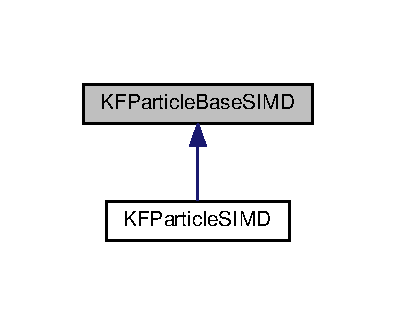
\includegraphics[width=190pt]{classKFParticleBaseSIMD__inherit__graph}
\end{center}
\end{figure}
\subsection*{Public Member Functions}
\begin{DoxyCompactItemize}
\item 
void $\ast$ \hyperlink{classKFParticleBaseSIMD_ade85c0c5ee22ae3ed7645f19fa3738ba}{operator new} (size\+\_\+t size)\hypertarget{classKFParticleBaseSIMD_ade85c0c5ee22ae3ed7645f19fa3738ba}{}\label{classKFParticleBaseSIMD_ade85c0c5ee22ae3ed7645f19fa3738ba}

\begin{DoxyCompactList}\small\item\em new operator for allocation of the S\+I\+M\+D-\/alligned dynamic memory allocation \end{DoxyCompactList}\item 
void $\ast$ \hyperlink{classKFParticleBaseSIMD_a207da9048fff76dd51b14d3a2a2a8156}{operator new\mbox{[}$\,$\mbox{]}} (size\+\_\+t size)\hypertarget{classKFParticleBaseSIMD_a207da9048fff76dd51b14d3a2a2a8156}{}\label{classKFParticleBaseSIMD_a207da9048fff76dd51b14d3a2a2a8156}

\begin{DoxyCompactList}\small\item\em new operator for allocation of the S\+I\+M\+D-\/alligned dynamic memory allocation \end{DoxyCompactList}\item 
void $\ast$ \hyperlink{classKFParticleBaseSIMD_a95ffdc0b1bcf20ac50fd17679320d788}{operator new} (size\+\_\+t size, void $\ast$ptr)\hypertarget{classKFParticleBaseSIMD_a95ffdc0b1bcf20ac50fd17679320d788}{}\label{classKFParticleBaseSIMD_a95ffdc0b1bcf20ac50fd17679320d788}

\begin{DoxyCompactList}\small\item\em new operator for allocation of the S\+I\+M\+D-\/alligned dynamic memory allocation \end{DoxyCompactList}\item 
void $\ast$ \hyperlink{classKFParticleBaseSIMD_a299c4dc0cd49e862c48ec445e2657e17}{operator new\mbox{[}$\,$\mbox{]}} (size\+\_\+t size, void $\ast$ptr)\hypertarget{classKFParticleBaseSIMD_a299c4dc0cd49e862c48ec445e2657e17}{}\label{classKFParticleBaseSIMD_a299c4dc0cd49e862c48ec445e2657e17}

\begin{DoxyCompactList}\small\item\em new operator for allocation of the S\+I\+M\+D-\/alligned dynamic memory allocation \end{DoxyCompactList}\item 
void \hyperlink{classKFParticleBaseSIMD_ab859077e6894489885e064ef08de02be}{operator delete} (void $\ast$ptr, size\+\_\+t)\hypertarget{classKFParticleBaseSIMD_ab859077e6894489885e064ef08de02be}{}\label{classKFParticleBaseSIMD_ab859077e6894489885e064ef08de02be}

\begin{DoxyCompactList}\small\item\em delete operator for the S\+I\+M\+D-\/alligned dynamic memory release \end{DoxyCompactList}\item 
void \hyperlink{classKFParticleBaseSIMD_aead161ff9e6fc09d603794105177c503}{operator delete\mbox{[}$\,$\mbox{]}} (void $\ast$ptr, size\+\_\+t)\hypertarget{classKFParticleBaseSIMD_aead161ff9e6fc09d603794105177c503}{}\label{classKFParticleBaseSIMD_aead161ff9e6fc09d603794105177c503}

\begin{DoxyCompactList}\small\item\em delete operator for the S\+I\+M\+D-\/alligned dynamic memory release \end{DoxyCompactList}\item 
virtual void \hyperlink{classKFParticleBaseSIMD_a63891fb44fb5a375907e67a7d048d970}{Get\+Field\+Value} (const float\+\_\+v xyz\mbox{[}$\,$\mbox{]}, float\+\_\+v B\mbox{[}$\,$\mbox{]}) const =0
\item 
virtual float\+\_\+v \hyperlink{classKFParticleBaseSIMD_a762391583bafd7f932bc80fbd226bce5}{Get\+D\+Sto\+Point} (const float\+\_\+v xyz\mbox{[}3\mbox{]}, float\+\_\+v dsdr\mbox{[}6\mbox{]}) const =0
\item 
float\+\_\+v \hyperlink{classKFParticleBaseSIMD_abae627fc1bb1e7439826d12d14a6d379}{Get\+D\+Sto\+Point\+Line} (const float\+\_\+v xyz\mbox{[}3\mbox{]}, float\+\_\+v dsdr\mbox{[}6\mbox{]}) const 
\item 
float\+\_\+v \hyperlink{classKFParticleBaseSIMD_a1ebeaf16c037b7cbb1c8d05848be1fbe}{Get\+D\+Sto\+Point\+Bz} (float\+\_\+v Bz, const float\+\_\+v xyz\mbox{[}3\mbox{]}, float\+\_\+v dsdr\mbox{[}6\mbox{]}, const float\+\_\+v $\ast$param=nullptr) const 
\item 
float\+\_\+v \hyperlink{classKFParticleBaseSIMD_a59e8050469c4aa5bb1920d8426543b4b}{Get\+D\+Sto\+Point\+By} (float\+\_\+v By, const float\+\_\+v xyz\mbox{[}3\mbox{]}, float\+\_\+v dsdr\mbox{[}6\mbox{]}) const 
\item 
float\+\_\+v \hyperlink{classKFParticleBaseSIMD_a1dbb5988ec5d1507a2b6d229cf761eb4}{Get\+D\+Sto\+Point\+C\+BM} (const float\+\_\+v xyz\mbox{[}3\mbox{]}, float\+\_\+v dsdr\mbox{[}6\mbox{]}) const 
\item 
virtual void \hyperlink{classKFParticleBaseSIMD_af386cf32fdc113792305a1f38f2683c7}{Get\+D\+Sto\+Particle} (const \hyperlink{classKFParticleBaseSIMD}{K\+F\+Particle\+Base\+S\+I\+MD} \&p, float\+\_\+v dS\mbox{[}2\mbox{]}, float\+\_\+v dsdr\mbox{[}4\mbox{]}\mbox{[}6\mbox{]}) const =0
\item 
virtual void \hyperlink{classKFParticleBaseSIMD_afeee016bf203bca0bd17959509541334}{Get\+D\+Sto\+Particle\+Fast} (const \hyperlink{classKFParticleBaseSIMD}{K\+F\+Particle\+Base\+S\+I\+MD} \&p, float\+\_\+v dS\mbox{[}2\mbox{]}) const =0
\item 
void \hyperlink{classKFParticleBaseSIMD_a8e96d6b648dbc125f44f3a6e54844df7}{Get\+D\+Sto\+Particle\+Line} (const \hyperlink{classKFParticleBaseSIMD}{K\+F\+Particle\+Base\+S\+I\+MD} \&p, float\+\_\+v dS\mbox{[}2\mbox{]}, float\+\_\+v dsdr\mbox{[}4\mbox{]}\mbox{[}6\mbox{]}) const 
\item 
void \hyperlink{classKFParticleBaseSIMD_a9a7028feaf50340f96452a3fa75159e0}{Get\+D\+Sto\+Particle\+Line} (const \hyperlink{classKFParticleBaseSIMD}{K\+F\+Particle\+Base\+S\+I\+MD} \&p, float\+\_\+v dS\mbox{[}2\mbox{]}) const 
\item 
void \hyperlink{classKFParticleBaseSIMD_af48beb91cdace844ed70ae927d31c96e}{Get\+D\+Sto\+Particle\+Bz} (float\+\_\+v Bz, const \hyperlink{classKFParticleBaseSIMD}{K\+F\+Particle\+Base\+S\+I\+MD} \&p, float\+\_\+v dS\mbox{[}2\mbox{]}, float\+\_\+v dsdr\mbox{[}4\mbox{]}\mbox{[}6\mbox{]}, const float\+\_\+v $\ast$param1=nullptr, const float\+\_\+v $\ast$param2=nullptr) const 
\item 
void \hyperlink{classKFParticleBaseSIMD_a067e1b2914968999024912bbe1b741ef}{Get\+D\+Sto\+Particle\+Bz} (float\+\_\+v Bz, const \hyperlink{classKFParticleBaseSIMD}{K\+F\+Particle\+Base\+S\+I\+MD} \&p, float\+\_\+v dS\mbox{[}2\mbox{]}, const float\+\_\+v $\ast$param1=nullptr, const float\+\_\+v $\ast$param2=nullptr) const 
\item 
void \hyperlink{classKFParticleBaseSIMD_a807794fa31286b74663338e91a515e28}{Get\+D\+Sto\+Particle\+By} (float\+\_\+v B, const \hyperlink{classKFParticleBaseSIMD}{K\+F\+Particle\+Base\+S\+I\+MD} \&p, float\+\_\+v dS\mbox{[}2\mbox{]}, float\+\_\+v dsdr\mbox{[}4\mbox{]}\mbox{[}6\mbox{]}) const 
\item 
void \hyperlink{classKFParticleBaseSIMD_a53e483c36be41f4b2b31167079448c50}{Get\+D\+Sto\+Particle\+By} (float\+\_\+v B, const \hyperlink{classKFParticleBaseSIMD}{K\+F\+Particle\+Base\+S\+I\+MD} \&p, float\+\_\+v dS\mbox{[}2\mbox{]}) const 
\item 
void \hyperlink{classKFParticleBaseSIMD_af18dabf64aa93effd00e8ef3187df1e8}{Get\+D\+Sto\+ParticleB} (float\+\_\+v B\mbox{[}3\mbox{]}, const \hyperlink{classKFParticleBaseSIMD}{K\+F\+Particle\+Base\+S\+I\+MD} \&p, float\+\_\+v dS\mbox{[}2\mbox{]}, float\+\_\+v dsdr\mbox{[}4\mbox{]}\mbox{[}6\mbox{]}) const 
\item 
void \hyperlink{classKFParticleBaseSIMD_a1b4d0c9300c389abefe0315f45faa26b}{Get\+D\+Sto\+ParticleB} (float\+\_\+v B\mbox{[}3\mbox{]}, const \hyperlink{classKFParticleBaseSIMD}{K\+F\+Particle\+Base\+S\+I\+MD} \&p, float\+\_\+v dS\mbox{[}2\mbox{]}) const 
\item 
void \hyperlink{classKFParticleBaseSIMD_acd7097a1ad5f82efff3812c01580e592}{Get\+D\+Sto\+Particle\+C\+BM} (const \hyperlink{classKFParticleBaseSIMD}{K\+F\+Particle\+Base\+S\+I\+MD} \&p, float\+\_\+v dS\mbox{[}2\mbox{]}, float\+\_\+v dsdr\mbox{[}4\mbox{]}\mbox{[}6\mbox{]}) const 
\item 
void \hyperlink{classKFParticleBaseSIMD_a0dd9de9d7915fd843abc49ffc9b53da1}{Get\+D\+Sto\+Particle\+C\+BM} (const \hyperlink{classKFParticleBaseSIMD}{K\+F\+Particle\+Base\+S\+I\+MD} \&p, float\+\_\+v dS\mbox{[}2\mbox{]}) const 
\item 
virtual void \hyperlink{classKFParticleBaseSIMD_aef008a05ee4b4c5c8fc88a8e7493ee70}{Transport} (float\+\_\+v dS, const float\+\_\+v dsdr\mbox{[}6\mbox{]}, float\+\_\+v P\mbox{[}$\,$\mbox{]}, float\+\_\+v C\mbox{[}$\,$\mbox{]}, float\+\_\+v $\ast$dsdr1=nullptr, float\+\_\+v $\ast$F=nullptr, float\+\_\+v $\ast$F1=nullptr) const =0
\item 
virtual void \hyperlink{classKFParticleBaseSIMD_a20c50860d7bc9f4e2c1047f8028320d1}{Transport\+Fast} (float\+\_\+v dS, float\+\_\+v P\mbox{[}$\,$\mbox{]}) const =0
\item 
\hyperlink{classKFParticleBaseSIMD_a6d298c2dfdaf132412630d18fbc0e94c}{K\+F\+Particle\+Base\+S\+I\+MD} ()
\item 
virtual \hyperlink{classKFParticleBaseSIMD_a8af269cd0effa0f4eaa7b7933b28c456}{$\sim$\+K\+F\+Particle\+Base\+S\+I\+MD} ()\hypertarget{classKFParticleBaseSIMD_a8af269cd0effa0f4eaa7b7933b28c456}{}\label{classKFParticleBaseSIMD_a8af269cd0effa0f4eaa7b7933b28c456}

\begin{DoxyCompactList}\small\item\em The default destructor. \end{DoxyCompactList}\item 
void \hyperlink{classKFParticleBaseSIMD_a20da6183e6320e398d5df7d72ff1ad8c}{Initialize} (const float\+\_\+v Param\mbox{[}$\,$\mbox{]}, const float\+\_\+v Cov\mbox{[}$\,$\mbox{]}, int\+\_\+v Charge, float\+\_\+v Mass)
\item 
void \hyperlink{classKFParticleBaseSIMD_a6fea58bda9e030e5ebee1b24e27efb46}{Initialize} ()
\item 
void \hyperlink{classKFParticleBaseSIMD_a51bd465905712fb71a33a9b7c20b966f}{Set\+Construct\+Method} (Int\+\_\+t m)\hypertarget{classKFParticleBaseSIMD_a51bd465905712fb71a33a9b7c20b966f}{}\label{classKFParticleBaseSIMD_a51bd465905712fb71a33a9b7c20b966f}

\begin{DoxyCompactList}\small\item\em Defines the construction method for the current particle (see description of f\+Construct\+Method). \end{DoxyCompactList}\item 
void \hyperlink{classKFParticleBaseSIMD_a85cd002f960edc11de214421f0ec00b4}{Set\+Mass\+Hypo} (float\+\_\+v m)\hypertarget{classKFParticleBaseSIMD_a85cd002f960edc11de214421f0ec00b4}{}\label{classKFParticleBaseSIMD_a85cd002f960edc11de214421f0ec00b4}

\begin{DoxyCompactList}\small\item\em Sets the mass hypothesis to the particle, is used when f\+Construct\+Method = 2. \end{DoxyCompactList}\item 
const float\+\_\+v \& \hyperlink{classKFParticleBaseSIMD_ab30c31111824d87b88bfc02c53fcaec1}{Get\+Mass\+Hypo} () const \hypertarget{classKFParticleBaseSIMD_ab30c31111824d87b88bfc02c53fcaec1}{}\label{classKFParticleBaseSIMD_ab30c31111824d87b88bfc02c53fcaec1}

\begin{DoxyCompactList}\small\item\em Returns the mass hypothesis. \end{DoxyCompactList}\item 
const float\+\_\+v \& \hyperlink{classKFParticleBaseSIMD_a3b50e6fdc8b56aed187da4eec3936afe}{Get\+Sum\+Daughter\+Mass} () const \hypertarget{classKFParticleBaseSIMD_a3b50e6fdc8b56aed187da4eec3936afe}{}\label{classKFParticleBaseSIMD_a3b50e6fdc8b56aed187da4eec3936afe}

\begin{DoxyCompactList}\small\item\em Returns the sum of masses of the daughters. \end{DoxyCompactList}\item 
float\+\_\+v \hyperlink{classKFParticleBaseSIMD_a6b2c3d26757c9d1b1ac2f2dbaa0b3415}{GetX} () const \hypertarget{classKFParticleBaseSIMD_a6b2c3d26757c9d1b1ac2f2dbaa0b3415}{}\label{classKFParticleBaseSIMD_a6b2c3d26757c9d1b1ac2f2dbaa0b3415}

\begin{DoxyCompactList}\small\item\em Returns the sum of masses of the daughters. \end{DoxyCompactList}\item 
float\+\_\+v \hyperlink{classKFParticleBaseSIMD_a2bec26d0571f001feb2288519aa2ca67}{GetY} () const \hypertarget{classKFParticleBaseSIMD_a2bec26d0571f001feb2288519aa2ca67}{}\label{classKFParticleBaseSIMD_a2bec26d0571f001feb2288519aa2ca67}

\begin{DoxyCompactList}\small\item\em Returns the sum of masses of the daughters. \end{DoxyCompactList}\item 
float\+\_\+v \hyperlink{classKFParticleBaseSIMD_a3c6b3dbb664b880c348ac6fb0f715e85}{GetZ} () const \hypertarget{classKFParticleBaseSIMD_a3c6b3dbb664b880c348ac6fb0f715e85}{}\label{classKFParticleBaseSIMD_a3c6b3dbb664b880c348ac6fb0f715e85}

\begin{DoxyCompactList}\small\item\em Returns the sum of masses of the daughters. \end{DoxyCompactList}\item 
float\+\_\+v \hyperlink{classKFParticleBaseSIMD_adf7d8c12dcfa4f8696d83326847f4b48}{Get\+Px} () const \hypertarget{classKFParticleBaseSIMD_adf7d8c12dcfa4f8696d83326847f4b48}{}\label{classKFParticleBaseSIMD_adf7d8c12dcfa4f8696d83326847f4b48}

\begin{DoxyCompactList}\small\item\em Returns the sum of masses of the daughters. \end{DoxyCompactList}\item 
float\+\_\+v \hyperlink{classKFParticleBaseSIMD_aabb7573a7dd045b4b9c2762e5a626159}{Get\+Py} () const \hypertarget{classKFParticleBaseSIMD_aabb7573a7dd045b4b9c2762e5a626159}{}\label{classKFParticleBaseSIMD_aabb7573a7dd045b4b9c2762e5a626159}

\begin{DoxyCompactList}\small\item\em Returns the sum of masses of the daughters. \end{DoxyCompactList}\item 
float\+\_\+v \hyperlink{classKFParticleBaseSIMD_a829cb413174d40b78bf34f14fd536619}{Get\+Pz} () const \hypertarget{classKFParticleBaseSIMD_a829cb413174d40b78bf34f14fd536619}{}\label{classKFParticleBaseSIMD_a829cb413174d40b78bf34f14fd536619}

\begin{DoxyCompactList}\small\item\em Returns the sum of masses of the daughters. \end{DoxyCompactList}\item 
float\+\_\+v \hyperlink{classKFParticleBaseSIMD_aa15f73c7c6691e04911d32cb9b16ef9b}{GetE} () const \hypertarget{classKFParticleBaseSIMD_aa15f73c7c6691e04911d32cb9b16ef9b}{}\label{classKFParticleBaseSIMD_aa15f73c7c6691e04911d32cb9b16ef9b}

\begin{DoxyCompactList}\small\item\em Returns the sum of masses of the daughters. \end{DoxyCompactList}\item 
float\+\_\+v \hyperlink{classKFParticleBaseSIMD_ae4125f86727f05cf6689c35c8dc3f947}{GetS} () const \hypertarget{classKFParticleBaseSIMD_ae4125f86727f05cf6689c35c8dc3f947}{}\label{classKFParticleBaseSIMD_ae4125f86727f05cf6689c35c8dc3f947}

\begin{DoxyCompactList}\small\item\em Returns the sum of masses of the daughters. \end{DoxyCompactList}\item 
int\+\_\+v \hyperlink{classKFParticleBaseSIMD_a926d1ef18075badaf63d0241a673d644}{GetQ} () const \hypertarget{classKFParticleBaseSIMD_a926d1ef18075badaf63d0241a673d644}{}\label{classKFParticleBaseSIMD_a926d1ef18075badaf63d0241a673d644}

\begin{DoxyCompactList}\small\item\em Returns the sum of masses of the daughters. \end{DoxyCompactList}\item 
float\+\_\+v \hyperlink{classKFParticleBaseSIMD_ab8734826c2ff3a13b524cee16a65e55b}{Get\+Chi2} () const \hypertarget{classKFParticleBaseSIMD_ab8734826c2ff3a13b524cee16a65e55b}{}\label{classKFParticleBaseSIMD_ab8734826c2ff3a13b524cee16a65e55b}

\begin{DoxyCompactList}\small\item\em Returns the sum of masses of the daughters. \end{DoxyCompactList}\item 
int\+\_\+v \hyperlink{classKFParticleBaseSIMD_ad64dccb1e5b0fb94842e8a28e5037b31}{Get\+N\+DF} () const \hypertarget{classKFParticleBaseSIMD_ad64dccb1e5b0fb94842e8a28e5037b31}{}\label{classKFParticleBaseSIMD_ad64dccb1e5b0fb94842e8a28e5037b31}

\begin{DoxyCompactList}\small\item\em Returns the sum of masses of the daughters. \end{DoxyCompactList}\item 
const float\+\_\+v \& \hyperlink{classKFParticleBaseSIMD_ad2188b32c30eaa4822f9f8ee0312c262}{X} () const \hypertarget{classKFParticleBaseSIMD_ad2188b32c30eaa4822f9f8ee0312c262}{}\label{classKFParticleBaseSIMD_ad2188b32c30eaa4822f9f8ee0312c262}

\begin{DoxyCompactList}\small\item\em Retruns X coordinate of the particle, fP\mbox{[}0\mbox{]}. \end{DoxyCompactList}\item 
const float\+\_\+v \& \hyperlink{classKFParticleBaseSIMD_a0317637c84246ec7f34accf35c9cb8fd}{Y} () const \hypertarget{classKFParticleBaseSIMD_a0317637c84246ec7f34accf35c9cb8fd}{}\label{classKFParticleBaseSIMD_a0317637c84246ec7f34accf35c9cb8fd}

\begin{DoxyCompactList}\small\item\em Retruns Y coordinate of the particle, fP\mbox{[}1\mbox{]}. \end{DoxyCompactList}\item 
const float\+\_\+v \& \hyperlink{classKFParticleBaseSIMD_a3189c60d84706832532e315723dca770}{Z} () const \hypertarget{classKFParticleBaseSIMD_a3189c60d84706832532e315723dca770}{}\label{classKFParticleBaseSIMD_a3189c60d84706832532e315723dca770}

\begin{DoxyCompactList}\small\item\em Retruns Z coordinate of the particle, fP\mbox{[}2\mbox{]}. \end{DoxyCompactList}\item 
const float\+\_\+v \& \hyperlink{classKFParticleBaseSIMD_a3695da551e4329333ba60889472954bf}{Px} () const \hypertarget{classKFParticleBaseSIMD_a3695da551e4329333ba60889472954bf}{}\label{classKFParticleBaseSIMD_a3695da551e4329333ba60889472954bf}

\begin{DoxyCompactList}\small\item\em Retruns X component of the momentum, fP\mbox{[}3\mbox{]}. \end{DoxyCompactList}\item 
const float\+\_\+v \& \hyperlink{classKFParticleBaseSIMD_a567654c96e90393a47a5e48e95aed117}{Py} () const \hypertarget{classKFParticleBaseSIMD_a567654c96e90393a47a5e48e95aed117}{}\label{classKFParticleBaseSIMD_a567654c96e90393a47a5e48e95aed117}

\begin{DoxyCompactList}\small\item\em Retruns Y component of the momentum, fP\mbox{[}4\mbox{]}. \end{DoxyCompactList}\item 
const float\+\_\+v \& \hyperlink{classKFParticleBaseSIMD_a4ac015d5658f6874d0e769b3d2eb7b9a}{Pz} () const \hypertarget{classKFParticleBaseSIMD_a4ac015d5658f6874d0e769b3d2eb7b9a}{}\label{classKFParticleBaseSIMD_a4ac015d5658f6874d0e769b3d2eb7b9a}

\begin{DoxyCompactList}\small\item\em Retruns Z component of the momentum, fP\mbox{[}5\mbox{]}. \end{DoxyCompactList}\item 
const float\+\_\+v \& \hyperlink{classKFParticleBaseSIMD_a4bd7f392f848910230c1c0bd8daf3d65}{E} () const \hypertarget{classKFParticleBaseSIMD_a4bd7f392f848910230c1c0bd8daf3d65}{}\label{classKFParticleBaseSIMD_a4bd7f392f848910230c1c0bd8daf3d65}

\begin{DoxyCompactList}\small\item\em Returns energy of the particle, fP\mbox{[}6\mbox{]}. \end{DoxyCompactList}\item 
const float\+\_\+v \& \hyperlink{classKFParticleBaseSIMD_a906019dfd64d4209f9734506b195f9ed}{S} () const \hypertarget{classKFParticleBaseSIMD_a906019dfd64d4209f9734506b195f9ed}{}\label{classKFParticleBaseSIMD_a906019dfd64d4209f9734506b195f9ed}

\begin{DoxyCompactList}\small\item\em Returns dS=l/p, l -\/ decay length, fP\mbox{[}7\mbox{]}, defined if production vertex is set. \end{DoxyCompactList}\item 
const int\+\_\+v \& \hyperlink{classKFParticleBaseSIMD_a4627da237cb56fc359e983cf697741c0}{Q} () const \hypertarget{classKFParticleBaseSIMD_a4627da237cb56fc359e983cf697741c0}{}\label{classKFParticleBaseSIMD_a4627da237cb56fc359e983cf697741c0}

\begin{DoxyCompactList}\small\item\em Returns charge of the particle. \end{DoxyCompactList}\item 
const float\+\_\+v \& \hyperlink{classKFParticleBaseSIMD_a54e2c6e7835e73172da85839ca2c4753}{Chi2} () const \hypertarget{classKFParticleBaseSIMD_a54e2c6e7835e73172da85839ca2c4753}{}\label{classKFParticleBaseSIMD_a54e2c6e7835e73172da85839ca2c4753}

\begin{DoxyCompactList}\small\item\em Returns Chi2 of the fit. \end{DoxyCompactList}\item 
const int\+\_\+v \& \hyperlink{classKFParticleBaseSIMD_a52b5ff420b0fe125c2b53651565d5e28}{N\+DF} () const \hypertarget{classKFParticleBaseSIMD_a52b5ff420b0fe125c2b53651565d5e28}{}\label{classKFParticleBaseSIMD_a52b5ff420b0fe125c2b53651565d5e28}

\begin{DoxyCompactList}\small\item\em Returns number of decrease of freedom. \end{DoxyCompactList}\item 
float\+\_\+v \hyperlink{classKFParticleBaseSIMD_aedb30f3be0ee8f5da98feaabe9d3074e}{Get\+Parameter} (Int\+\_\+t i) const \hypertarget{classKFParticleBaseSIMD_aedb30f3be0ee8f5da98feaabe9d3074e}{}\label{classKFParticleBaseSIMD_aedb30f3be0ee8f5da98feaabe9d3074e}

\begin{DoxyCompactList}\small\item\em Returns P\mbox{[}i\mbox{]} parameter. \end{DoxyCompactList}\item 
float\+\_\+v \hyperlink{classKFParticleBaseSIMD_a4f7b481e281eb3b0bfc45cfb7db1065c}{Get\+Covariance} (Int\+\_\+t i) const \hypertarget{classKFParticleBaseSIMD_a4f7b481e281eb3b0bfc45cfb7db1065c}{}\label{classKFParticleBaseSIMD_a4f7b481e281eb3b0bfc45cfb7db1065c}

\begin{DoxyCompactList}\small\item\em Returns C\mbox{[}i\mbox{]} element of the covariance matrix in the lower triangular form. \end{DoxyCompactList}\item 
float\+\_\+v \hyperlink{classKFParticleBaseSIMD_aba80c9e268af07473fcf0aa75c804507}{Get\+Covariance} (Int\+\_\+t i, Int\+\_\+t j) const \hypertarget{classKFParticleBaseSIMD_aba80c9e268af07473fcf0aa75c804507}{}\label{classKFParticleBaseSIMD_aba80c9e268af07473fcf0aa75c804507}

\begin{DoxyCompactList}\small\item\em Returns C\mbox{[}i,j\mbox{]} element of the covariance matrix. \end{DoxyCompactList}\item 
float\+\_\+m \hyperlink{classKFParticleBaseSIMD_a7ef771f44d5ef1b9ec3cd6a05567f0f1}{Get\+Momentum} (float\+\_\+v \&p, float\+\_\+v \&error) const 
\item 
float\+\_\+m \hyperlink{classKFParticleBaseSIMD_a2be75da924159255f3dc954e0e6a3271}{Get\+Pt} (float\+\_\+v \&pt, float\+\_\+v \&error) const 
\item 
float\+\_\+m \hyperlink{classKFParticleBaseSIMD_ab67bce164eba1fa6e68b8ffc2eac6e7f}{Get\+Eta} (float\+\_\+v \&eta, float\+\_\+v \&error) const 
\item 
float\+\_\+m \hyperlink{classKFParticleBaseSIMD_a94c1bacdec14ef93110b1dfb141073ad}{Get\+Phi} (float\+\_\+v \&phi, float\+\_\+v \&error) const 
\item 
float\+\_\+m \hyperlink{classKFParticleBaseSIMD_ac8690a32660c0f65990b10c875c2f2af}{Get\+Mass} (float\+\_\+v \&m, float\+\_\+v \&error) const 
\item 
float\+\_\+m \hyperlink{classKFParticleBaseSIMD_a74a930684c0796e5925365cb27a01730}{Get\+Decay\+Length} (float\+\_\+v \&l, float\+\_\+v \&error) const 
\item 
float\+\_\+m \hyperlink{classKFParticleBaseSIMD_a36d374972632038adb3c40d2413af473}{Get\+Decay\+Length\+XY} (float\+\_\+v \&l, float\+\_\+v \&error) const 
\item 
float\+\_\+m \hyperlink{classKFParticleBaseSIMD_afcf43ad8f2972af95843614f71073df8}{Get\+Life\+Time} (float\+\_\+v \&ctau, float\+\_\+v \&error) const 
\item 
float\+\_\+m \hyperlink{classKFParticleBaseSIMD_a39b53aee81bd8fa790629afbf8777804}{GetR} (float\+\_\+v \&r, float\+\_\+v \&error) const 
\item 
float\+\_\+v \& \hyperlink{classKFParticleBaseSIMD_ad595a2d626eaa6bd262e8cfe7e8a4dc4}{X} ()\hypertarget{classKFParticleBaseSIMD_ad595a2d626eaa6bd262e8cfe7e8a4dc4}{}\label{classKFParticleBaseSIMD_ad595a2d626eaa6bd262e8cfe7e8a4dc4}

\begin{DoxyCompactList}\small\item\em Modifier of X coordinate of the particle, fP\mbox{[}0\mbox{]}. \end{DoxyCompactList}\item 
float\+\_\+v \& \hyperlink{classKFParticleBaseSIMD_af9ee57d22217d5adb101c19d944ef437}{Y} ()\hypertarget{classKFParticleBaseSIMD_af9ee57d22217d5adb101c19d944ef437}{}\label{classKFParticleBaseSIMD_af9ee57d22217d5adb101c19d944ef437}

\begin{DoxyCompactList}\small\item\em Modifier of Y coordinate of the particle, fP\mbox{[}1\mbox{]}. \end{DoxyCompactList}\item 
float\+\_\+v \& \hyperlink{classKFParticleBaseSIMD_ad89b52dfe1f528db45a5a0c672103f04}{Z} ()\hypertarget{classKFParticleBaseSIMD_ad89b52dfe1f528db45a5a0c672103f04}{}\label{classKFParticleBaseSIMD_ad89b52dfe1f528db45a5a0c672103f04}

\begin{DoxyCompactList}\small\item\em Modifier of Z coordinate of the particle, fP\mbox{[}2\mbox{]}. \end{DoxyCompactList}\item 
float\+\_\+v \& \hyperlink{classKFParticleBaseSIMD_a7b9f51c18e0e6166c713d02379ebbb36}{Px} ()\hypertarget{classKFParticleBaseSIMD_a7b9f51c18e0e6166c713d02379ebbb36}{}\label{classKFParticleBaseSIMD_a7b9f51c18e0e6166c713d02379ebbb36}

\begin{DoxyCompactList}\small\item\em Modifier of X component of the momentum, fP\mbox{[}3\mbox{]}. \end{DoxyCompactList}\item 
float\+\_\+v \& \hyperlink{classKFParticleBaseSIMD_a98e7aec5396e91e5d061b84950eae29a}{Py} ()\hypertarget{classKFParticleBaseSIMD_a98e7aec5396e91e5d061b84950eae29a}{}\label{classKFParticleBaseSIMD_a98e7aec5396e91e5d061b84950eae29a}

\begin{DoxyCompactList}\small\item\em Modifier of Y component of the momentum, fP\mbox{[}4\mbox{]}. \end{DoxyCompactList}\item 
float\+\_\+v \& \hyperlink{classKFParticleBaseSIMD_a16e2c66877a779ea2c557177eb255224}{Pz} ()\hypertarget{classKFParticleBaseSIMD_a16e2c66877a779ea2c557177eb255224}{}\label{classKFParticleBaseSIMD_a16e2c66877a779ea2c557177eb255224}

\begin{DoxyCompactList}\small\item\em Modifier of Z component of the momentum, fP\mbox{[}5\mbox{]}. \end{DoxyCompactList}\item 
float\+\_\+v \& \hyperlink{classKFParticleBaseSIMD_a46d69ecf9cd0c6bbc1a848d5a8e1ae0b}{E} ()\hypertarget{classKFParticleBaseSIMD_a46d69ecf9cd0c6bbc1a848d5a8e1ae0b}{}\label{classKFParticleBaseSIMD_a46d69ecf9cd0c6bbc1a848d5a8e1ae0b}

\begin{DoxyCompactList}\small\item\em Modifier of energy of the particle, fP\mbox{[}6\mbox{]}. \end{DoxyCompactList}\item 
float\+\_\+v \& \hyperlink{classKFParticleBaseSIMD_ad15ac850401a548df731453f35db64dd}{S} ()\hypertarget{classKFParticleBaseSIMD_ad15ac850401a548df731453f35db64dd}{}\label{classKFParticleBaseSIMD_ad15ac850401a548df731453f35db64dd}

\begin{DoxyCompactList}\small\item\em Modifier of dS=l/p, l -\/ decay length, fP\mbox{[}7\mbox{]}, defined if production vertex is set. \end{DoxyCompactList}\item 
int\+\_\+v \& \hyperlink{classKFParticleBaseSIMD_a710ce08809b254aac583349705151973}{Q} ()\hypertarget{classKFParticleBaseSIMD_a710ce08809b254aac583349705151973}{}\label{classKFParticleBaseSIMD_a710ce08809b254aac583349705151973}

\begin{DoxyCompactList}\small\item\em Modifier of charge of the particle. \end{DoxyCompactList}\item 
float\+\_\+v \& \hyperlink{classKFParticleBaseSIMD_ae203be3b49c5af07d2ee3d895a2f21dc}{Chi2} ()\hypertarget{classKFParticleBaseSIMD_ae203be3b49c5af07d2ee3d895a2f21dc}{}\label{classKFParticleBaseSIMD_ae203be3b49c5af07d2ee3d895a2f21dc}

\begin{DoxyCompactList}\small\item\em Modifier of Chi2 of the fit. \end{DoxyCompactList}\item 
int\+\_\+v \& \hyperlink{classKFParticleBaseSIMD_a7e8c6fe04118c9dce503cea711011ee0}{N\+DF} ()\hypertarget{classKFParticleBaseSIMD_a7e8c6fe04118c9dce503cea711011ee0}{}\label{classKFParticleBaseSIMD_a7e8c6fe04118c9dce503cea711011ee0}

\begin{DoxyCompactList}\small\item\em Modifier of number of decrease of freedom. \end{DoxyCompactList}\item 
float\+\_\+v \& \hyperlink{classKFParticleBaseSIMD_ad876a667b7e64c2177a7b06866c3260c}{Parameter} (Int\+\_\+t i)\hypertarget{classKFParticleBaseSIMD_ad876a667b7e64c2177a7b06866c3260c}{}\label{classKFParticleBaseSIMD_ad876a667b7e64c2177a7b06866c3260c}

\begin{DoxyCompactList}\small\item\em Modifier of P\mbox{[}i\mbox{]} parameter. \end{DoxyCompactList}\item 
float\+\_\+v \& \hyperlink{classKFParticleBaseSIMD_a4243bcff049f640d8f78da88f17e20db}{Covariance} (Int\+\_\+t i)\hypertarget{classKFParticleBaseSIMD_a4243bcff049f640d8f78da88f17e20db}{}\label{classKFParticleBaseSIMD_a4243bcff049f640d8f78da88f17e20db}

\begin{DoxyCompactList}\small\item\em Modifier of C\mbox{[}i\mbox{]} element of the covariance matrix in the lower triangular form. \end{DoxyCompactList}\item 
float\+\_\+v \& \hyperlink{classKFParticleBaseSIMD_a0c2df01356d9cbd2b7a762096c8e5a20}{Covariance} (Int\+\_\+t i, Int\+\_\+t j)\hypertarget{classKFParticleBaseSIMD_a0c2df01356d9cbd2b7a762096c8e5a20}{}\label{classKFParticleBaseSIMD_a0c2df01356d9cbd2b7a762096c8e5a20}

\begin{DoxyCompactList}\small\item\em Modifier of C\mbox{[}i,j\mbox{]} element of the covariance matrix. \end{DoxyCompactList}\item 
void \hyperlink{classKFParticleBaseSIMD_a2cc73a1a3812b9e58ab777131d74b058}{operator+=} (const \hyperlink{classKFParticleBaseSIMD}{K\+F\+Particle\+Base\+S\+I\+MD} \&Daughter)
\item 
void \hyperlink{classKFParticleBaseSIMD_a2ee0cc29dedac6767db45ae197a0fe35}{Add\+Daughter} (const \hyperlink{classKFParticleBaseSIMD}{K\+F\+Particle\+Base\+S\+I\+MD} \&Daughter)
\item 
void \hyperlink{classKFParticleBaseSIMD_afce83e9f433c1ccc698197ae2ffe36d4}{Subtract\+Daughter} (const \hyperlink{classKFParticleBaseSIMD}{K\+F\+Particle\+Base\+S\+I\+MD} \&Daughter)
\item 
void \hyperlink{classKFParticleBaseSIMD_a31bbbd45b75df2d238522b1607ee5726}{Add\+Daughter\+With\+Energy\+Fit} (const \hyperlink{classKFParticleBaseSIMD}{K\+F\+Particle\+Base\+S\+I\+MD} \&Daughter)
\item 
void \hyperlink{classKFParticleBaseSIMD_affe2b18e82526005b6f34cd213a1f579}{Add\+Daughter\+With\+Energy\+Fit\+MC} (const \hyperlink{classKFParticleBaseSIMD}{K\+F\+Particle\+Base\+S\+I\+MD} \&Daughter)
\item 
void \hyperlink{classKFParticleBaseSIMD_ab9370932a09a02d6498ca4c960caba13}{Set\+Production\+Vertex} (const \hyperlink{classKFParticleBaseSIMD}{K\+F\+Particle\+Base\+S\+I\+MD} \&Vtx)
\item 
void \hyperlink{classKFParticleBaseSIMD_a5583455557dbd2de22cc0adbee47b3be}{Set\+Nonlinear\+Mass\+Constraint} (float\+\_\+v Mass)
\item 
void \hyperlink{classKFParticleBaseSIMD_af05cfb05f0e552e283dd0cdc33c92327}{Set\+Mass\+Constraint} (float\+\_\+v Mass, float\+\_\+v Sigma\+Mass=float\+\_\+v(0.f))
\item 
void \hyperlink{classKFParticleBaseSIMD_a21beb9923513d2ec67d0d00a1b232d96}{Set\+No\+Decay\+Length} ()
\item 
void \hyperlink{classKFParticleBaseSIMD_a768c539d5e5a59f6425d9eed0c1b1545}{Construct} (const \hyperlink{classKFParticleBaseSIMD}{K\+F\+Particle\+Base\+S\+I\+MD} $\ast$v\+Daughters\mbox{[}$\,$\mbox{]}, Int\+\_\+t n\+Daughters, const \hyperlink{classKFParticleBaseSIMD}{K\+F\+Particle\+Base\+S\+I\+MD} $\ast$Prod\+Vtx=nullptr, Float\+\_\+t Mass=-\/1)
\item 
void \hyperlink{classKFParticleBaseSIMD_a1163dac578cd40f360f1778ceb880035}{Transport\+To\+Decay\+Vertex} ()
\item 
void \hyperlink{classKFParticleBaseSIMD_a0a6f09356d3e2a3cfdc3637090ed10dd}{Transport\+To\+Production\+Vertex} ()
\item 
void \hyperlink{classKFParticleBaseSIMD_ae4bd5b9ffbeb8b5f9595cf6d34592c31}{Transport\+To\+DS} (float\+\_\+v dS, const float\+\_\+v $\ast$dsdr)
\item 
void \hyperlink{classKFParticleBaseSIMD_a01255a2f9bd979672aa08041cf2b34a4}{Transport\+To\+D\+S\+Line} (float\+\_\+v dS, const float\+\_\+v $\ast$dsdr)
\item 
void \hyperlink{classKFParticleBaseSIMD_a4acde83e522366bef474e49f7f2509c7}{Transport\+Bz} (float\+\_\+v Bz, float\+\_\+v dS, const float\+\_\+v $\ast$dsdr, float\+\_\+v P\mbox{[}$\,$\mbox{]}, float\+\_\+v C\mbox{[}$\,$\mbox{]}, float\+\_\+v $\ast$dsdr1=nullptr, float\+\_\+v $\ast$F=nullptr, float\+\_\+v $\ast$F1=nullptr) const 
\item 
void \hyperlink{classKFParticleBaseSIMD_acb05aa525f9794f635fc113dc724548d}{Transport\+Bz} (float\+\_\+v Bz, float\+\_\+v dS, float\+\_\+v P\mbox{[}$\,$\mbox{]}) const 
\item 
void \hyperlink{classKFParticleBaseSIMD_a0fb8ef971518781a8205d08220159321}{Transport\+C\+BM} (float\+\_\+v dS, const float\+\_\+v $\ast$dsdr, float\+\_\+v P\mbox{[}$\,$\mbox{]}, float\+\_\+v C\mbox{[}$\,$\mbox{]}, float\+\_\+v $\ast$dsdr1=nullptr, float\+\_\+v $\ast$F=nullptr, float\+\_\+v $\ast$F1=nullptr) const 
\item 
void \hyperlink{classKFParticleBaseSIMD_a314c83fd7be746bebb954e1a558faa12}{Transport\+C\+BM} (float\+\_\+v dS, float\+\_\+v P\mbox{[}$\,$\mbox{]}) const 
\item 
float\+\_\+v \hyperlink{classKFParticleBaseSIMD_adfb65cfc48f2e66e3a1cb55c85c5b53e}{Get\+Distance\+From\+Vertex} (const float\+\_\+v vtx\mbox{[}$\,$\mbox{]}) const 
\item 
float\+\_\+v \hyperlink{classKFParticleBaseSIMD_a63ace5a90b37dd5271b33d4b6a5e63a6}{Get\+Distance\+From\+Vertex} (const \hyperlink{classKFParticleBaseSIMD}{K\+F\+Particle\+Base\+S\+I\+MD} \&Vtx) const 
\item 
float\+\_\+v \hyperlink{classKFParticleBaseSIMD_a7c0a29adffcefb49d4b3ccb2d8ffc1d3}{Get\+Distance\+From\+Particle} (const \hyperlink{classKFParticleBaseSIMD}{K\+F\+Particle\+Base\+S\+I\+MD} \&p) const 
\item 
float\+\_\+v \hyperlink{classKFParticleBaseSIMD_af290fc3494b3a4cf039a322b85d2170c}{Get\+Deviation\+From\+Vertex} (const float\+\_\+v v\mbox{[}$\,$\mbox{]}, const float\+\_\+v Cv\mbox{[}$\,$\mbox{]}=nullptr) const 
\item 
float\+\_\+v \hyperlink{classKFParticleBaseSIMD_a43d3005745f3c408f2cf6296e72870b3}{Get\+Deviation\+From\+Vertex} (const \hyperlink{classKFParticleBaseSIMD}{K\+F\+Particle\+Base\+S\+I\+MD} \&Vtx) const 
\item 
float\+\_\+v \hyperlink{classKFParticleBaseSIMD_a2f5e730fa0ac84f5ac2559b5a358328b}{Get\+Deviation\+From\+Particle} (const \hyperlink{classKFParticleBaseSIMD}{K\+F\+Particle\+Base\+S\+I\+MD} \&p) const 
\item 
void \hyperlink{classKFParticleBaseSIMD_a15202c15c0476824b316a7edc5783ca0}{Subtract\+From\+Vertex} (\hyperlink{classKFParticleBaseSIMD}{K\+F\+Particle\+Base\+S\+I\+MD} \&Vtx) const 
\item 
void \hyperlink{classKFParticleBaseSIMD_ad7bdaa7cad85e3157f53aedc60a9f2d8}{Subtract\+From\+Particle} (\hyperlink{classKFParticleBaseSIMD}{K\+F\+Particle\+Base\+S\+I\+MD} \&Vtx) const 
\item 
void \hyperlink{classKFParticleBaseSIMD_a2fc8aa6e9722f33468d0d1817bda46d9}{Rotate\+XY} (float\+\_\+v angle, float\+\_\+v Vtx\mbox{[}3\mbox{]})
\item 
int\+\_\+v \hyperlink{classKFParticleBaseSIMD_a4f43f26357ae4a6e35ca5b8e4a1d623f}{Id} () const \hypertarget{classKFParticleBaseSIMD_a4f43f26357ae4a6e35ca5b8e4a1d623f}{}\label{classKFParticleBaseSIMD_a4f43f26357ae4a6e35ca5b8e4a1d623f}

\begin{DoxyCompactList}\small\item\em Returns Id of the particle. \end{DoxyCompactList}\item 
int \hyperlink{classKFParticleBaseSIMD_a575650529485dfca810314581d68e469}{N\+Daughters} () const \hypertarget{classKFParticleBaseSIMD_a575650529485dfca810314581d68e469}{}\label{classKFParticleBaseSIMD_a575650529485dfca810314581d68e469}

\begin{DoxyCompactList}\small\item\em Returns number of daughter particles. \end{DoxyCompactList}\item 
std\+::vector$<$ int\+\_\+v $>$ \& \hyperlink{classKFParticleBaseSIMD_ac827f191d739ef99b5bee7ebc97d5313}{Daughter\+Ids} ()\hypertarget{classKFParticleBaseSIMD_ac827f191d739ef99b5bee7ebc97d5313}{}\label{classKFParticleBaseSIMD_ac827f191d739ef99b5bee7ebc97d5313}

\begin{DoxyCompactList}\small\item\em Returns the vector with the indices of daughter particles. \end{DoxyCompactList}\item 
int\+\_\+v \hyperlink{classKFParticleBaseSIMD_ac57b8345a161bd445b3cea5bc23b0210}{Get\+Daughter\+Id} (int iD) const \hypertarget{classKFParticleBaseSIMD_ac57b8345a161bd445b3cea5bc23b0210}{}\label{classKFParticleBaseSIMD_ac57b8345a161bd445b3cea5bc23b0210}

\begin{DoxyCompactList}\small\item\em Returns the daughter Id with the index iD. \end{DoxyCompactList}\item 
void \hyperlink{classKFParticleBaseSIMD_a81cd387d3cf24a498205ebb4bea5e9ff}{Set\+Id} (int\+\_\+v id)\hypertarget{classKFParticleBaseSIMD_a81cd387d3cf24a498205ebb4bea5e9ff}{}\label{classKFParticleBaseSIMD_a81cd387d3cf24a498205ebb4bea5e9ff}

\begin{DoxyCompactList}\small\item\em Sets the Id of the particle. After the construction of a particle should be set by user. \end{DoxyCompactList}\item 
void \hyperlink{classKFParticleBaseSIMD_a2ae7f872e011430fb8db5eae6488e776}{Set\+N\+Daughters} (int n)\hypertarget{classKFParticleBaseSIMD_a2ae7f872e011430fb8db5eae6488e776}{}\label{classKFParticleBaseSIMD_a2ae7f872e011430fb8db5eae6488e776}

\begin{DoxyCompactList}\small\item\em Reserves the size of the vector with daughter Ids to n. \end{DoxyCompactList}\item 
void \hyperlink{classKFParticleBaseSIMD_a7e60f55ad9b21a9a196c3ad08a46a52d}{Add\+Daughter\+Id} (int\+\_\+v id)\hypertarget{classKFParticleBaseSIMD_a7e60f55ad9b21a9a196c3ad08a46a52d}{}\label{classKFParticleBaseSIMD_a7e60f55ad9b21a9a196c3ad08a46a52d}

\begin{DoxyCompactList}\small\item\em Adds index of the daughter particle. \end{DoxyCompactList}\item 
void \hyperlink{classKFParticleBaseSIMD_a3eeb37388f866c06bee751d3ac31f9da}{Clean\+Daughters\+Id} ()\hypertarget{classKFParticleBaseSIMD_a3eeb37388f866c06bee751d3ac31f9da}{}\label{classKFParticleBaseSIMD_a3eeb37388f866c06bee751d3ac31f9da}

\begin{DoxyCompactList}\small\item\em Cleans the vector with the indices of daughter particles. \end{DoxyCompactList}\item 
void \hyperlink{classKFParticleBaseSIMD_a86e624a4194a7de352389e659b720f90}{Set\+P\+DG} (int pdg)\hypertarget{classKFParticleBaseSIMD_a86e624a4194a7de352389e659b720f90}{}\label{classKFParticleBaseSIMD_a86e624a4194a7de352389e659b720f90}

\begin{DoxyCompactList}\small\item\em Sets the P\+DG hypothesis common for all elements of the S\+I\+MD vector. \end{DoxyCompactList}\item 
void \hyperlink{classKFParticleBaseSIMD_adbc541da175de9f39bf78707a82fe920}{Set\+P\+DG} (int\+\_\+v \&pdg)\hypertarget{classKFParticleBaseSIMD_adbc541da175de9f39bf78707a82fe920}{}\label{classKFParticleBaseSIMD_adbc541da175de9f39bf78707a82fe920}

\begin{DoxyCompactList}\small\item\em Sets the P\+DG hypothesis individual for each entry of the S\+I\+MD vector. \end{DoxyCompactList}\item 
const int\+\_\+v \& \hyperlink{classKFParticleBaseSIMD_a34e19ecaaedf374a347e648eca770ca9}{Get\+P\+DG} () const \hypertarget{classKFParticleBaseSIMD_a34e19ecaaedf374a347e648eca770ca9}{}\label{classKFParticleBaseSIMD_a34e19ecaaedf374a347e648eca770ca9}

\begin{DoxyCompactList}\small\item\em Returns the P\+DG hypothesis. \end{DoxyCompactList}\item 
const int\+\_\+v \& \hyperlink{classKFParticleBaseSIMD_a4d481ddc56411eb602a83003188a33fb}{P\+DG} () const \hypertarget{classKFParticleBaseSIMD_a4d481ddc56411eb602a83003188a33fb}{}\label{classKFParticleBaseSIMD_a4d481ddc56411eb602a83003188a33fb}

\begin{DoxyCompactList}\small\item\em Returns the P\+DG hypothesis. \end{DoxyCompactList}\item 
void \hyperlink{classKFParticleBaseSIMD_a915415876b3372299216507b55399629}{Get\+Distance\+To\+Vertex\+Line} (const \hyperlink{classKFParticleBaseSIMD}{K\+F\+Particle\+Base\+S\+I\+MD} \&Vertex, float\+\_\+v \&l, float\+\_\+v \&dl, float\+\_\+m $\ast$is\+Particle\+From\+Vertex=nullptr) const 
\end{DoxyCompactItemize}
\subsection*{Static Public Member Functions}
\begin{DoxyCompactItemize}
\item 
static void \hyperlink{classKFParticleBaseSIMD_a2ddfa6bbbd4b147886b484d88b5d0e07}{Get\+Armenteros\+Podolanski} (\hyperlink{classKFParticleBaseSIMD}{K\+F\+Particle\+Base\+S\+I\+MD} \&positive, \hyperlink{classKFParticleBaseSIMD}{K\+F\+Particle\+Base\+S\+I\+MD} \&negative, float\+\_\+v Qt\+Alfa\mbox{[}2\mbox{]})
\item 
static void \hyperlink{classKFParticleBaseSIMD_a1339b5e3c8989903017e88a267fd5da3}{Mult\+Q\+S\+Qt} (const float\+\_\+v \hyperlink{classKFParticleBaseSIMD_a4627da237cb56fc359e983cf697741c0}{Q}\mbox{[}$\,$\mbox{]}, const float\+\_\+v \hyperlink{classKFParticleBaseSIMD_a906019dfd64d4209f9734506b195f9ed}{S}\mbox{[}$\,$\mbox{]}, float\+\_\+v S\+Out\mbox{[}$\,$\mbox{]}, int kN)
\end{DoxyCompactItemize}
\subsection*{Protected Member Functions}
\begin{DoxyCompactItemize}
\item 
float\+\_\+v \& \hyperlink{classKFParticleBaseSIMD_accd0d91999cad3409e82272a976cc878}{Cij} (Int\+\_\+t i, Int\+\_\+t j)
\item 
void \hyperlink{classKFParticleBaseSIMD_a22e86d6a0599f96326ea022bc8e84deb}{Transport\+Line} (float\+\_\+v \hyperlink{classKFParticleBaseSIMD_a906019dfd64d4209f9734506b195f9ed}{S}, const float\+\_\+v $\ast$dsdr, float\+\_\+v P\mbox{[}$\,$\mbox{]}, float\+\_\+v C\mbox{[}$\,$\mbox{]}, float\+\_\+v $\ast$dsdr1=nullptr, float\+\_\+v $\ast$F=nullptr, float\+\_\+v $\ast$F1=nullptr) const 
\item 
void \hyperlink{classKFParticleBaseSIMD_ab95a02fa9f64b2a299986623aae3e09b}{Transport\+Line} (float\+\_\+v \hyperlink{classKFParticleBaseSIMD_a906019dfd64d4209f9734506b195f9ed}{S}, float\+\_\+v P\mbox{[}$\,$\mbox{]}) const 
\item 
void \hyperlink{classKFParticleBaseSIMD_abead77d712c9ce7ed12bd925c5fb3d8b}{Get\+Measurement} (const \hyperlink{classKFParticleBaseSIMD}{K\+F\+Particle\+Base\+S\+I\+MD} \&daughter, float\+\_\+v m\mbox{[}$\,$\mbox{]}, float\+\_\+v V\mbox{[}$\,$\mbox{]}, float\+\_\+v D\mbox{[}3\mbox{]}\mbox{[}3\mbox{]})
\end{DoxyCompactItemize}
\subsection*{Static Protected Member Functions}
\begin{DoxyCompactItemize}
\item 
static Int\+\_\+t \hyperlink{classKFParticleBaseSIMD_a23c8f9fa65a42b162990806191f91148}{IJ} (Int\+\_\+t i, Int\+\_\+t j)
\item 
static void \hyperlink{classKFParticleBaseSIMD_a4050fd23fd4493d83633bb00a312522b}{Invert\+Choletsky3} (float\+\_\+v a\mbox{[}6\mbox{]})
\item 
static void \hyperlink{classKFParticleBaseSIMD_a64947e4a11a881b3a36da3e5d529d99f}{Set\+Mass\+Constraint} (float\+\_\+v $\ast$mP, float\+\_\+v $\ast$mC, float\+\_\+v mJ\mbox{[}7\mbox{]}\mbox{[}7\mbox{]}, float\+\_\+v mass, float\+\_\+m mask)
\end{DoxyCompactItemize}
\subsection*{Protected Attributes}
\begin{DoxyCompactItemize}
\item 
float\+\_\+v \hyperlink{classKFParticleBaseSIMD_a112eb61d3426e5fa2f98a73fb6f2c8e8}{fP} \mbox{[}8\mbox{]}\hypertarget{classKFParticleBaseSIMD_a112eb61d3426e5fa2f98a73fb6f2c8e8}{}\label{classKFParticleBaseSIMD_a112eb61d3426e5fa2f98a73fb6f2c8e8}

\begin{DoxyCompactList}\small\item\em Particle parameters \{ X, Y, Z, Px, Py, Pz, E, S\mbox{[}=Decay\+Length/P\mbox{]}\}. \end{DoxyCompactList}\item 
float\+\_\+v \hyperlink{classKFParticleBaseSIMD_a0a2d89649f3876d56874e4373b1be5b1}{fC} \mbox{[}36\mbox{]}\hypertarget{classKFParticleBaseSIMD_a0a2d89649f3876d56874e4373b1be5b1}{}\label{classKFParticleBaseSIMD_a0a2d89649f3876d56874e4373b1be5b1}

\begin{DoxyCompactList}\small\item\em Low-\/triangle covariance matrix of fP. \end{DoxyCompactList}\item 
int\+\_\+v \hyperlink{classKFParticleBaseSIMD_a94025d7ab80d0ed5c663a3292f534b15}{fQ}\hypertarget{classKFParticleBaseSIMD_a94025d7ab80d0ed5c663a3292f534b15}{}\label{classKFParticleBaseSIMD_a94025d7ab80d0ed5c663a3292f534b15}

\begin{DoxyCompactList}\small\item\em The charge of the particle in the units of the elementary charge. \end{DoxyCompactList}\item 
int\+\_\+v \hyperlink{classKFParticleBaseSIMD_ad51213e8e023679f60016f428b08a220}{f\+N\+DF}\hypertarget{classKFParticleBaseSIMD_ad51213e8e023679f60016f428b08a220}{}\label{classKFParticleBaseSIMD_ad51213e8e023679f60016f428b08a220}

\begin{DoxyCompactList}\small\item\em Number of degrees of freedom. \end{DoxyCompactList}\item 
float\+\_\+v \hyperlink{classKFParticleBaseSIMD_adba176e03b9eadb9494eded3e7a77b59}{f\+Chi2}\hypertarget{classKFParticleBaseSIMD_adba176e03b9eadb9494eded3e7a77b59}{}\label{classKFParticleBaseSIMD_adba176e03b9eadb9494eded3e7a77b59}

\begin{DoxyCompactList}\small\item\em Chi$^\wedge$2. \end{DoxyCompactList}\item 
float\+\_\+v \hyperlink{classKFParticleBaseSIMD_a98512ef37c7e4601482403b30d47cb38}{f\+S\+From\+Decay}\hypertarget{classKFParticleBaseSIMD_a98512ef37c7e4601482403b30d47cb38}{}\label{classKFParticleBaseSIMD_a98512ef37c7e4601482403b30d47cb38}

\begin{DoxyCompactList}\small\item\em Distance from the decay vertex to the current position. \end{DoxyCompactList}\item 
float\+\_\+v \hyperlink{classKFParticleBaseSIMD_afd3f256956cf1ac57cfd88589f1a6646}{Sum\+Daughter\+Mass}\hypertarget{classKFParticleBaseSIMD_afd3f256956cf1ac57cfd88589f1a6646}{}\label{classKFParticleBaseSIMD_afd3f256956cf1ac57cfd88589f1a6646}

\begin{DoxyCompactList}\small\item\em Sum of the daughter particles masses. Needed to set the constraint on the minimum mass during particle construction. \end{DoxyCompactList}\item 
float\+\_\+v \hyperlink{classKFParticleBaseSIMD_a7ec69eabb247fa58c6e4e562cce38bdb}{f\+Mass\+Hypo}\hypertarget{classKFParticleBaseSIMD_a7ec69eabb247fa58c6e4e562cce38bdb}{}\label{classKFParticleBaseSIMD_a7ec69eabb247fa58c6e4e562cce38bdb}

\begin{DoxyCompactList}\small\item\em The mass hypothesis, used for the constraints during particle construction. \end{DoxyCompactList}\item 
int\+\_\+v \hyperlink{classKFParticleBaseSIMD_ac72c5bee98e7eed297bc7c01ba51f735}{f\+Id}\hypertarget{classKFParticleBaseSIMD_ac72c5bee98e7eed297bc7c01ba51f735}{}\label{classKFParticleBaseSIMD_ac72c5bee98e7eed297bc7c01ba51f735}

\begin{DoxyCompactList}\small\item\em Id of the particle. \end{DoxyCompactList}\item 
Bool\+\_\+t \hyperlink{classKFParticleBaseSIMD_a696499e57fbc18e3e95678c937e29035}{f\+At\+Production\+Vertex}\hypertarget{classKFParticleBaseSIMD_a696499e57fbc18e3e95678c937e29035}{}\label{classKFParticleBaseSIMD_a696499e57fbc18e3e95678c937e29035}

\begin{DoxyCompactList}\small\item\em Flag shows if particle is at the production point. \end{DoxyCompactList}\item 
int\+\_\+v \hyperlink{classKFParticleBaseSIMD_a80a98ddcb03c9ef62e78257c8dbffe2d}{f\+P\+DG}\hypertarget{classKFParticleBaseSIMD_a80a98ddcb03c9ef62e78257c8dbffe2d}{}\label{classKFParticleBaseSIMD_a80a98ddcb03c9ef62e78257c8dbffe2d}

\begin{DoxyCompactList}\small\item\em The P\+DG hypothesis assigned to the particle. \end{DoxyCompactList}\item 
Int\+\_\+t \hyperlink{classKFParticleBaseSIMD_a509a7ba63eb251b7f40e2282a4754377}{f\+Construct\+Method}\hypertarget{classKFParticleBaseSIMD_a509a7ba63eb251b7f40e2282a4754377}{}\label{classKFParticleBaseSIMD_a509a7ba63eb251b7f40e2282a4754377}

\begin{DoxyCompactList}\small\item\em Determines the method for the particle construction. ~\newline
0 -\/ Energy considered as an independent veriable, fitted independently from momentum, without any constraints on mass ~\newline
2 -\/ Energy considered as an independent variable, fitted independently from momentum, with constraints on mass of daughter particle. \end{DoxyCompactList}\item 
std\+::vector$<$ int\+\_\+v $>$ \hyperlink{classKFParticleBaseSIMD_ac8e0407b65c920d778068278468e5343}{f\+Daughter\+Ids}\hypertarget{classKFParticleBaseSIMD_ac8e0407b65c920d778068278468e5343}{}\label{classKFParticleBaseSIMD_ac8e0407b65c920d778068278468e5343}

\begin{DoxyCompactList}\small\item\em A vector with ids of the daughter particles\+: ~\newline
1) if particle is created from a track -\/ the index of the track, in this case the size of the vector is always equal to one; ~\newline
2) if particle is constructed from other particles -\/ indices of these particles in the same array. \end{DoxyCompactList}\end{DoxyCompactItemize}


\subsection{Detailed Description}
The base of \hyperlink{classKFParticleSIMD}{K\+F\+Particle\+S\+I\+MD} class. 

\begin{DoxyAuthor}{Author}
M.\+Zyzak 
\end{DoxyAuthor}
\begin{DoxyDate}{Date}
05.\+02.\+2019 
\end{DoxyDate}
\begin{DoxyVersion}{Version}
1.\+0
\end{DoxyVersion}
Contains the main mathematics of the vectorised KF Particle. Will be merged with the \hyperlink{classKFParticleSIMD}{K\+F\+Particle\+S\+I\+MD} class. The class stores all the data in a format of S\+I\+MD vectors, the mathematics is fully vectorised. T\+He mathematics is implemented in single precision. The functionality of the vectorised and scalar classes is the same. 

\subsection{Constructor \& Destructor Documentation}
\index{K\+F\+Particle\+Base\+S\+I\+MD@{K\+F\+Particle\+Base\+S\+I\+MD}!K\+F\+Particle\+Base\+S\+I\+MD@{K\+F\+Particle\+Base\+S\+I\+MD}}
\index{K\+F\+Particle\+Base\+S\+I\+MD@{K\+F\+Particle\+Base\+S\+I\+MD}!K\+F\+Particle\+Base\+S\+I\+MD@{K\+F\+Particle\+Base\+S\+I\+MD}}
\subsubsection[{\texorpdfstring{K\+F\+Particle\+Base\+S\+I\+M\+D()}{KFParticleBaseSIMD()}}]{\setlength{\rightskip}{0pt plus 5cm}K\+F\+Particle\+Base\+S\+I\+M\+D\+::\+K\+F\+Particle\+Base\+S\+I\+MD (
\begin{DoxyParamCaption}
{}
\end{DoxyParamCaption}
)}\hypertarget{classKFParticleBaseSIMD_a6d298c2dfdaf132412630d18fbc0e94c}{}\label{classKFParticleBaseSIMD_a6d298c2dfdaf132412630d18fbc0e94c}
The default constructor, initialises the parameters by\+: ~\newline
1) all parameters are set to 0; ~\newline
2) all elements of the covariance matrix are set to 0 except Cxx=Cyy=Czz=100; ~\newline
3) Q = 0; ~\newline
4) chi2 is set to 0; ~\newline
5) N\+DF = -\/3, since 3 parameters should be fitted\+: X, Y, Z.

\subsection{Member Function Documentation}
\index{K\+F\+Particle\+Base\+S\+I\+MD@{K\+F\+Particle\+Base\+S\+I\+MD}!Add\+Daughter@{Add\+Daughter}}
\index{Add\+Daughter@{Add\+Daughter}!K\+F\+Particle\+Base\+S\+I\+MD@{K\+F\+Particle\+Base\+S\+I\+MD}}
\subsubsection[{\texorpdfstring{Add\+Daughter(const K\+F\+Particle\+Base\+S\+I\+M\+D \&\+Daughter)}{AddDaughter(const KFParticleBaseSIMD &Daughter)}}]{\setlength{\rightskip}{0pt plus 5cm}void K\+F\+Particle\+Base\+S\+I\+M\+D\+::\+Add\+Daughter (
\begin{DoxyParamCaption}
\item[{const {\bf K\+F\+Particle\+Base\+S\+I\+MD} \&}]{Daughter}
\end{DoxyParamCaption}
)}\hypertarget{classKFParticleBaseSIMD_a2ee0cc29dedac6767db45ae197a0fe35}{}\label{classKFParticleBaseSIMD_a2ee0cc29dedac6767db45ae197a0fe35}
Adds daughter to the current particle. Depending on the selected construction method uses\+: ~\newline
1) Either simplifyed fast mathematics which consideres momentum and energy as independent variables and thus ignores constraint on the fixed mass (f\+Construct\+Method = 0). In this case the mass of the daughter particle can be corrupted when the constructed vertex is added as the measurement and the mass of the output short-\/lived particle can become unphysical -\/ smaller then the threshold. Implemented in the \hyperlink{classKFParticleBaseSIMD_a31bbbd45b75df2d238522b1607ee5726}{Add\+Daughter\+With\+Energy\+Fit()} function ~\newline
2) Or slower but correct mathematics which requires that the masses of daughter particles stays fixed in the construction process (f\+Construct\+Method = 2). Implemented in the \hyperlink{classKFParticleBaseSIMD_affe2b18e82526005b6f34cd213a1f579}{Add\+Daughter\+With\+Energy\+Fit\+M\+C()} function. 
\begin{DoxyParams}[1]{Parameters}
\mbox{\tt in}  & {\em Daughter} & -\/ the daughter particle\\
\hline
\end{DoxyParams}
\index{K\+F\+Particle\+Base\+S\+I\+MD@{K\+F\+Particle\+Base\+S\+I\+MD}!Add\+Daughter\+With\+Energy\+Fit@{Add\+Daughter\+With\+Energy\+Fit}}
\index{Add\+Daughter\+With\+Energy\+Fit@{Add\+Daughter\+With\+Energy\+Fit}!K\+F\+Particle\+Base\+S\+I\+MD@{K\+F\+Particle\+Base\+S\+I\+MD}}
\subsubsection[{\texorpdfstring{Add\+Daughter\+With\+Energy\+Fit(const K\+F\+Particle\+Base\+S\+I\+M\+D \&\+Daughter)}{AddDaughterWithEnergyFit(const KFParticleBaseSIMD &Daughter)}}]{\setlength{\rightskip}{0pt plus 5cm}void K\+F\+Particle\+Base\+S\+I\+M\+D\+::\+Add\+Daughter\+With\+Energy\+Fit (
\begin{DoxyParamCaption}
\item[{const {\bf K\+F\+Particle\+Base\+S\+I\+MD} \&}]{Daughter}
\end{DoxyParamCaption}
)}\hypertarget{classKFParticleBaseSIMD_a31bbbd45b75df2d238522b1607ee5726}{}\label{classKFParticleBaseSIMD_a31bbbd45b75df2d238522b1607ee5726}
Adds daughter to the current particle. Uses simplifyed fast mathematics which consideres momentum and energy as independent variables and thus ignores constraint on the fixed mass. In this case the mass of the daughter particle can be corrupted when the constructed vertex is added as the measurement and the mass of the output short-\/lived particle can become unphysical -\/ smaller then the threshold. 
\begin{DoxyParams}[1]{Parameters}
\mbox{\tt in}  & {\em Daughter} & -\/ the daughter particle\\
\hline
\end{DoxyParams}
\index{K\+F\+Particle\+Base\+S\+I\+MD@{K\+F\+Particle\+Base\+S\+I\+MD}!Add\+Daughter\+With\+Energy\+Fit\+MC@{Add\+Daughter\+With\+Energy\+Fit\+MC}}
\index{Add\+Daughter\+With\+Energy\+Fit\+MC@{Add\+Daughter\+With\+Energy\+Fit\+MC}!K\+F\+Particle\+Base\+S\+I\+MD@{K\+F\+Particle\+Base\+S\+I\+MD}}
\subsubsection[{\texorpdfstring{Add\+Daughter\+With\+Energy\+Fit\+M\+C(const K\+F\+Particle\+Base\+S\+I\+M\+D \&\+Daughter)}{AddDaughterWithEnergyFitMC(const KFParticleBaseSIMD &Daughter)}}]{\setlength{\rightskip}{0pt plus 5cm}void K\+F\+Particle\+Base\+S\+I\+M\+D\+::\+Add\+Daughter\+With\+Energy\+Fit\+MC (
\begin{DoxyParamCaption}
\item[{const {\bf K\+F\+Particle\+Base\+S\+I\+MD} \&}]{Daughter}
\end{DoxyParamCaption}
)}\hypertarget{classKFParticleBaseSIMD_affe2b18e82526005b6f34cd213a1f579}{}\label{classKFParticleBaseSIMD_affe2b18e82526005b6f34cd213a1f579}
Adds daughter to the current particle. Uses slower but correct mathematics which requires that the masses of daughter particles stays fixed in the construction process. 
\begin{DoxyParams}[1]{Parameters}
\mbox{\tt in}  & {\em Daughter} & -\/ the daughter particle\\
\hline
\end{DoxyParams}
\index{K\+F\+Particle\+Base\+S\+I\+MD@{K\+F\+Particle\+Base\+S\+I\+MD}!Cij@{Cij}}
\index{Cij@{Cij}!K\+F\+Particle\+Base\+S\+I\+MD@{K\+F\+Particle\+Base\+S\+I\+MD}}
\subsubsection[{\texorpdfstring{Cij(\+Int\+\_\+t i, Int\+\_\+t j)}{Cij(Int_t i, Int_t j)}}]{\setlength{\rightskip}{0pt plus 5cm}float\+\_\+v\& K\+F\+Particle\+Base\+S\+I\+M\+D\+::\+Cij (
\begin{DoxyParamCaption}
\item[{Int\+\_\+t}]{i, }
\item[{Int\+\_\+t}]{j}
\end{DoxyParamCaption}
)\hspace{0.3cm}{\ttfamily [inline]}, {\ttfamily [protected]}}\hypertarget{classKFParticleBaseSIMD_accd0d91999cad3409e82272a976cc878}{}\label{classKFParticleBaseSIMD_accd0d91999cad3409e82272a976cc878}
Return an element of the covariance matrix with \{i,j\} indices. \index{K\+F\+Particle\+Base\+S\+I\+MD@{K\+F\+Particle\+Base\+S\+I\+MD}!Construct@{Construct}}
\index{Construct@{Construct}!K\+F\+Particle\+Base\+S\+I\+MD@{K\+F\+Particle\+Base\+S\+I\+MD}}
\subsubsection[{\texorpdfstring{Construct(const K\+F\+Particle\+Base\+S\+I\+M\+D $\ast$v\+Daughters[], Int\+\_\+t n\+Daughters, const K\+F\+Particle\+Base\+S\+I\+M\+D $\ast$\+Prod\+Vtx=nullptr, Float\+\_\+t Mass=-\/1)}{Construct(const KFParticleBaseSIMD *vDaughters[], Int_t nDaughters, const KFParticleBaseSIMD *ProdVtx=nullptr, Float_t Mass=-1)}}]{\setlength{\rightskip}{0pt plus 5cm}void K\+F\+Particle\+Base\+S\+I\+M\+D\+::\+Construct (
\begin{DoxyParamCaption}
\item[{const {\bf K\+F\+Particle\+Base\+S\+I\+MD} $\ast$}]{v\+Daughters\mbox{[}$\,$\mbox{]}, }
\item[{Int\+\_\+t}]{n\+Daughters, }
\item[{const {\bf K\+F\+Particle\+Base\+S\+I\+MD} $\ast$}]{Prod\+Vtx = {\ttfamily nullptr}, }
\item[{Float\+\_\+t}]{Mass = {\ttfamily -\/1}}
\end{DoxyParamCaption}
)}\hypertarget{classKFParticleBaseSIMD_a768c539d5e5a59f6425d9eed0c1b1545}{}\label{classKFParticleBaseSIMD_a768c539d5e5a59f6425d9eed0c1b1545}
Constructs a short-\/lived particle from a set of daughter particles\+:~\newline
1) all parameters of the \char`\"{}this\char`\"{} objects are initialised;~\newline
2) daughters are added one after another;~\newline
3) if Parent pointer is not null, the production vertex is set to it;~\newline
4) if Mass hypothesis $>$=0 the mass constraint is set. 
\begin{DoxyParams}[1]{Parameters}
\mbox{\tt in}  & {\em v\+Daughters} & -\/ array of daughter particles \\
\hline
\mbox{\tt in}  & {\em n\+Daughters} & -\/ number of daughter particles in the input array \\
\hline
\mbox{\tt in}  & {\em Parent} & -\/ optional parrent particle \\
\hline
\mbox{\tt in}  & {\em Mass} & -\/ optional mass hypothesis\\
\hline
\end{DoxyParams}
\index{K\+F\+Particle\+Base\+S\+I\+MD@{K\+F\+Particle\+Base\+S\+I\+MD}!Get\+Armenteros\+Podolanski@{Get\+Armenteros\+Podolanski}}
\index{Get\+Armenteros\+Podolanski@{Get\+Armenteros\+Podolanski}!K\+F\+Particle\+Base\+S\+I\+MD@{K\+F\+Particle\+Base\+S\+I\+MD}}
\subsubsection[{\texorpdfstring{Get\+Armenteros\+Podolanski(\+K\+F\+Particle\+Base\+S\+I\+M\+D \&positive, K\+F\+Particle\+Base\+S\+I\+M\+D \&negative, float\+\_\+v Qt\+Alfa[2])}{GetArmenterosPodolanski(KFParticleBaseSIMD &positive, KFParticleBaseSIMD &negative, float_v QtAlfa[2])}}]{\setlength{\rightskip}{0pt plus 5cm}void K\+F\+Particle\+Base\+S\+I\+M\+D\+::\+Get\+Armenteros\+Podolanski (
\begin{DoxyParamCaption}
\item[{{\bf K\+F\+Particle\+Base\+S\+I\+MD} \&}]{positive, }
\item[{{\bf K\+F\+Particle\+Base\+S\+I\+MD} \&}]{negative, }
\item[{float\+\_\+v}]{Qt\+Alfa\mbox{[}2\mbox{]}}
\end{DoxyParamCaption}
)\hspace{0.3cm}{\ttfamily [static]}}\hypertarget{classKFParticleBaseSIMD_a2ddfa6bbbd4b147886b484d88b5d0e07}{}\label{classKFParticleBaseSIMD_a2ddfa6bbbd4b147886b484d88b5d0e07}
Calculates parameters for the Armenteros-\/\+Podolanski plot for two particles. Example how to use\+:~\newline
\hyperlink{classKFParticle}{K\+F\+Particle} Pos\+Particle(...) ~\newline
\hyperlink{classKFParticle}{K\+F\+Particle} Neg\+Particle(...) ~\newline
Gamma.\+Construct\+Gamma(\+Pos\+Particle, Neg\+Particle); ~\newline
float Vertex\+Gamma\mbox{[}3\mbox{]} = \{Gamma.\+Get\+X(), Gamma.\+Get\+Y(), Gamma.\+Get\+Z()\}; ~\newline
Pos\+Particle.\+Transport\+To\+Point(\+Vertex\+Gamma); ~\newline
Neg\+Particle.\+Transport\+To\+Point(\+Vertex\+Gamma); ~\newline
float armenteros\+Qt\+Alfa\mbox{[}2\mbox{]} = \{0.\}; ~\newline
K\+F\+Particle\+::\+Get\+Armenteros\+Podolanski(\+Pos\+Particle, Neg\+Particle, armenteros\+Qt\+Alfa ); ~\newline

\begin{DoxyParams}[1]{Parameters}
\mbox{\tt in}  & {\em positive} & -\/ first particle, positive or neutral \\
\hline
\mbox{\tt in}  & {\em negative} & -\/ second particle, negative or neutral \\
\hline
\mbox{\tt out}  & {\em Qt\+Alfa\mbox{[}2\mbox{]}} & -\/ parameters for the Armenteros-\/\+Podolanski plot\+: Qt\+Alfa\mbox{[}0\mbox{]} = qt -\/ projection of the momenta of the particles on the transverse direction with respect to the total momentum, same for both particles; Qt\+Alfa\mbox{[}1\mbox{]} = (Pl+ -\/ Pl-\/)/(Pl+ + Pl-\/) -\/ combination of the longitudinal components.\\
\hline
\end{DoxyParams}
\index{K\+F\+Particle\+Base\+S\+I\+MD@{K\+F\+Particle\+Base\+S\+I\+MD}!Get\+Decay\+Length@{Get\+Decay\+Length}}
\index{Get\+Decay\+Length@{Get\+Decay\+Length}!K\+F\+Particle\+Base\+S\+I\+MD@{K\+F\+Particle\+Base\+S\+I\+MD}}
\subsubsection[{\texorpdfstring{Get\+Decay\+Length(float\+\_\+v \&l, float\+\_\+v \&error) const }{GetDecayLength(float_v &l, float_v &error) const }}]{\setlength{\rightskip}{0pt plus 5cm}float\+\_\+m K\+F\+Particle\+Base\+S\+I\+M\+D\+::\+Get\+Decay\+Length (
\begin{DoxyParamCaption}
\item[{float\+\_\+v \&}]{l, }
\item[{float\+\_\+v \&}]{error}
\end{DoxyParamCaption}
) const}\hypertarget{classKFParticleBaseSIMD_a74a930684c0796e5925365cb27a01730}{}\label{classKFParticleBaseSIMD_a74a930684c0796e5925365cb27a01730}
Calculates the decay length of the particle in the laboratory system and its error. If they are well defined the corresponding element of the return mask is set to 0, otherwise 1. The production point should be set before calling this function. 
\begin{DoxyParams}[1]{Parameters}
\mbox{\tt out}  & {\em l} & -\/ the decay length \\
\hline
\mbox{\tt out}  & {\em error} & -\/ its error\\
\hline
\end{DoxyParams}
\index{K\+F\+Particle\+Base\+S\+I\+MD@{K\+F\+Particle\+Base\+S\+I\+MD}!Get\+Decay\+Length\+XY@{Get\+Decay\+Length\+XY}}
\index{Get\+Decay\+Length\+XY@{Get\+Decay\+Length\+XY}!K\+F\+Particle\+Base\+S\+I\+MD@{K\+F\+Particle\+Base\+S\+I\+MD}}
\subsubsection[{\texorpdfstring{Get\+Decay\+Length\+X\+Y(float\+\_\+v \&l, float\+\_\+v \&error) const }{GetDecayLengthXY(float_v &l, float_v &error) const }}]{\setlength{\rightskip}{0pt plus 5cm}float\+\_\+m K\+F\+Particle\+Base\+S\+I\+M\+D\+::\+Get\+Decay\+Length\+XY (
\begin{DoxyParamCaption}
\item[{float\+\_\+v \&}]{l, }
\item[{float\+\_\+v \&}]{error}
\end{DoxyParamCaption}
) const}\hypertarget{classKFParticleBaseSIMD_a36d374972632038adb3c40d2413af473}{}\label{classKFParticleBaseSIMD_a36d374972632038adb3c40d2413af473}
Calculates the projection in the XY plane of the decay length of the particle in the laboratory system and its error. If they are well defined the corresponding element of the return mask is set to 0, otherwise 1. The production point should be set before calling this function. 
\begin{DoxyParams}[1]{Parameters}
\mbox{\tt out}  & {\em l} & -\/ the decay length \\
\hline
\mbox{\tt out}  & {\em error} & -\/ its error\\
\hline
\end{DoxyParams}
\index{K\+F\+Particle\+Base\+S\+I\+MD@{K\+F\+Particle\+Base\+S\+I\+MD}!Get\+Deviation\+From\+Particle@{Get\+Deviation\+From\+Particle}}
\index{Get\+Deviation\+From\+Particle@{Get\+Deviation\+From\+Particle}!K\+F\+Particle\+Base\+S\+I\+MD@{K\+F\+Particle\+Base\+S\+I\+MD}}
\subsubsection[{\texorpdfstring{Get\+Deviation\+From\+Particle(const K\+F\+Particle\+Base\+S\+I\+M\+D \&p) const }{GetDeviationFromParticle(const KFParticleBaseSIMD &p) const }}]{\setlength{\rightskip}{0pt plus 5cm}float\+\_\+v K\+F\+Particle\+Base\+S\+I\+M\+D\+::\+Get\+Deviation\+From\+Particle (
\begin{DoxyParamCaption}
\item[{const {\bf K\+F\+Particle\+Base\+S\+I\+MD} \&}]{p}
\end{DoxyParamCaption}
) const}\hypertarget{classKFParticleBaseSIMD_a2f5e730fa0ac84f5ac2559b5a358328b}{}\label{classKFParticleBaseSIMD_a2f5e730fa0ac84f5ac2559b5a358328b}
Returns Chi2 deviation of the current particle from another particle in 3D. 
\begin{DoxyParams}[1]{Parameters}
\mbox{\tt in}  & {\em p} & -\/ the second particle\\
\hline
\end{DoxyParams}
\index{K\+F\+Particle\+Base\+S\+I\+MD@{K\+F\+Particle\+Base\+S\+I\+MD}!Get\+Deviation\+From\+Vertex@{Get\+Deviation\+From\+Vertex}}
\index{Get\+Deviation\+From\+Vertex@{Get\+Deviation\+From\+Vertex}!K\+F\+Particle\+Base\+S\+I\+MD@{K\+F\+Particle\+Base\+S\+I\+MD}}
\subsubsection[{\texorpdfstring{Get\+Deviation\+From\+Vertex(const float\+\_\+v v[], const float\+\_\+v Cv[]=nullptr) const }{GetDeviationFromVertex(const float_v v[], const float_v Cv[]=nullptr) const }}]{\setlength{\rightskip}{0pt plus 5cm}float\+\_\+v K\+F\+Particle\+Base\+S\+I\+M\+D\+::\+Get\+Deviation\+From\+Vertex (
\begin{DoxyParamCaption}
\item[{const float\+\_\+v}]{v\mbox{[}$\,$\mbox{]}, }
\item[{const float\+\_\+v}]{Cv\mbox{[}$\,$\mbox{]} = {\ttfamily nullptr}}
\end{DoxyParamCaption}
) const}\hypertarget{classKFParticleBaseSIMD_af290fc3494b3a4cf039a322b85d2170c}{}\label{classKFParticleBaseSIMD_af290fc3494b3a4cf039a322b85d2170c}
Returns Chi2 deviation of the current particle from the vertex v with the covariance matrix Cv in 3D. 
\begin{DoxyParams}[1]{Parameters}
\mbox{\tt in}  & {\em v\mbox{[}3\mbox{]}} & -\/ coordinates of the vertex \{X, Y, Z\} \\
\hline
\mbox{\tt in}  & {\em Cv\mbox{[}6\mbox{]}} & -\/ covariance matrix of the vertex \{Cxx, Cxy, Cyy, Cxz, Czy, Czz\}\\
\hline
\end{DoxyParams}
\index{K\+F\+Particle\+Base\+S\+I\+MD@{K\+F\+Particle\+Base\+S\+I\+MD}!Get\+Deviation\+From\+Vertex@{Get\+Deviation\+From\+Vertex}}
\index{Get\+Deviation\+From\+Vertex@{Get\+Deviation\+From\+Vertex}!K\+F\+Particle\+Base\+S\+I\+MD@{K\+F\+Particle\+Base\+S\+I\+MD}}
\subsubsection[{\texorpdfstring{Get\+Deviation\+From\+Vertex(const K\+F\+Particle\+Base\+S\+I\+M\+D \&\+Vtx) const }{GetDeviationFromVertex(const KFParticleBaseSIMD &Vtx) const }}]{\setlength{\rightskip}{0pt plus 5cm}float\+\_\+v K\+F\+Particle\+Base\+S\+I\+M\+D\+::\+Get\+Deviation\+From\+Vertex (
\begin{DoxyParamCaption}
\item[{const {\bf K\+F\+Particle\+Base\+S\+I\+MD} \&}]{Vtx}
\end{DoxyParamCaption}
) const}\hypertarget{classKFParticleBaseSIMD_a43d3005745f3c408f2cf6296e72870b3}{}\label{classKFParticleBaseSIMD_a43d3005745f3c408f2cf6296e72870b3}
Returns Chi2 deviation of the current particle from the vertex in the \hyperlink{classKFParticle}{K\+F\+Particle} format in 3D. 
\begin{DoxyParams}[1]{Parameters}
\mbox{\tt in}  & {\em Vtx} & -\/ the vertex in K\+F\+Partcile format\\
\hline
\end{DoxyParams}
\index{K\+F\+Particle\+Base\+S\+I\+MD@{K\+F\+Particle\+Base\+S\+I\+MD}!Get\+Distance\+From\+Particle@{Get\+Distance\+From\+Particle}}
\index{Get\+Distance\+From\+Particle@{Get\+Distance\+From\+Particle}!K\+F\+Particle\+Base\+S\+I\+MD@{K\+F\+Particle\+Base\+S\+I\+MD}}
\subsubsection[{\texorpdfstring{Get\+Distance\+From\+Particle(const K\+F\+Particle\+Base\+S\+I\+M\+D \&p) const }{GetDistanceFromParticle(const KFParticleBaseSIMD &p) const }}]{\setlength{\rightskip}{0pt plus 5cm}float\+\_\+v K\+F\+Particle\+Base\+S\+I\+M\+D\+::\+Get\+Distance\+From\+Particle (
\begin{DoxyParamCaption}
\item[{const {\bf K\+F\+Particle\+Base\+S\+I\+MD} \&}]{p}
\end{DoxyParamCaption}
) const}\hypertarget{classKFParticleBaseSIMD_a7c0a29adffcefb49d4b3ccb2d8ffc1d3}{}\label{classKFParticleBaseSIMD_a7c0a29adffcefb49d4b3ccb2d8ffc1d3}
Returns the D\+CA distance from another particle p. 
\begin{DoxyParams}[1]{Parameters}
\mbox{\tt in}  & {\em p} & -\/ the second particle\\
\hline
\end{DoxyParams}
\index{K\+F\+Particle\+Base\+S\+I\+MD@{K\+F\+Particle\+Base\+S\+I\+MD}!Get\+Distance\+From\+Vertex@{Get\+Distance\+From\+Vertex}}
\index{Get\+Distance\+From\+Vertex@{Get\+Distance\+From\+Vertex}!K\+F\+Particle\+Base\+S\+I\+MD@{K\+F\+Particle\+Base\+S\+I\+MD}}
\subsubsection[{\texorpdfstring{Get\+Distance\+From\+Vertex(const float\+\_\+v vtx[]) const }{GetDistanceFromVertex(const float_v vtx[]) const }}]{\setlength{\rightskip}{0pt plus 5cm}float\+\_\+v K\+F\+Particle\+Base\+S\+I\+M\+D\+::\+Get\+Distance\+From\+Vertex (
\begin{DoxyParamCaption}
\item[{const float\+\_\+v}]{vtx\mbox{[}$\,$\mbox{]}}
\end{DoxyParamCaption}
) const}\hypertarget{classKFParticleBaseSIMD_adfb65cfc48f2e66e3a1cb55c85c5b53e}{}\label{classKFParticleBaseSIMD_adfb65cfc48f2e66e3a1cb55c85c5b53e}
Returns the D\+CA distance from vertex in 3D. 
\begin{DoxyParams}[1]{Parameters}
\mbox{\tt in}  & {\em vtx\mbox{[}3\mbox{]}} & -\/ the vertex coordinates \{X, Y, Z\}\\
\hline
\end{DoxyParams}
\index{K\+F\+Particle\+Base\+S\+I\+MD@{K\+F\+Particle\+Base\+S\+I\+MD}!Get\+Distance\+From\+Vertex@{Get\+Distance\+From\+Vertex}}
\index{Get\+Distance\+From\+Vertex@{Get\+Distance\+From\+Vertex}!K\+F\+Particle\+Base\+S\+I\+MD@{K\+F\+Particle\+Base\+S\+I\+MD}}
\subsubsection[{\texorpdfstring{Get\+Distance\+From\+Vertex(const K\+F\+Particle\+Base\+S\+I\+M\+D \&\+Vtx) const }{GetDistanceFromVertex(const KFParticleBaseSIMD &Vtx) const }}]{\setlength{\rightskip}{0pt plus 5cm}float\+\_\+v K\+F\+Particle\+Base\+S\+I\+M\+D\+::\+Get\+Distance\+From\+Vertex (
\begin{DoxyParamCaption}
\item[{const {\bf K\+F\+Particle\+Base\+S\+I\+MD} \&}]{Vtx}
\end{DoxyParamCaption}
) const}\hypertarget{classKFParticleBaseSIMD_a63ace5a90b37dd5271b33d4b6a5e63a6}{}\label{classKFParticleBaseSIMD_a63ace5a90b37dd5271b33d4b6a5e63a6}
Returns the D\+CA distance from vertex in the \hyperlink{classKFParticle}{K\+F\+Particle} format in 3D. 
\begin{DoxyParams}[1]{Parameters}
\mbox{\tt in}  & {\em Vtx} & -\/ the vertex in the \hyperlink{classKFParticle}{K\+F\+Particle} format\\
\hline
\end{DoxyParams}
\index{K\+F\+Particle\+Base\+S\+I\+MD@{K\+F\+Particle\+Base\+S\+I\+MD}!Get\+Distance\+To\+Vertex\+Line@{Get\+Distance\+To\+Vertex\+Line}}
\index{Get\+Distance\+To\+Vertex\+Line@{Get\+Distance\+To\+Vertex\+Line}!K\+F\+Particle\+Base\+S\+I\+MD@{K\+F\+Particle\+Base\+S\+I\+MD}}
\subsubsection[{\texorpdfstring{Get\+Distance\+To\+Vertex\+Line(const K\+F\+Particle\+Base\+S\+I\+M\+D \&\+Vertex, float\+\_\+v \&l, float\+\_\+v \&dl, float\+\_\+m $\ast$is\+Particle\+From\+Vertex=nullptr) const }{GetDistanceToVertexLine(const KFParticleBaseSIMD &Vertex, float_v &l, float_v &dl, float_m *isParticleFromVertex=nullptr) const }}]{\setlength{\rightskip}{0pt plus 5cm}void K\+F\+Particle\+Base\+S\+I\+M\+D\+::\+Get\+Distance\+To\+Vertex\+Line (
\begin{DoxyParamCaption}
\item[{const {\bf K\+F\+Particle\+Base\+S\+I\+MD} \&}]{Vertex, }
\item[{float\+\_\+v \&}]{l, }
\item[{float\+\_\+v \&}]{dl, }
\item[{float\+\_\+m $\ast$}]{is\+Particle\+From\+Vertex = {\ttfamily nullptr}}
\end{DoxyParamCaption}
) const}\hypertarget{classKFParticleBaseSIMD_a915415876b3372299216507b55399629}{}\label{classKFParticleBaseSIMD_a915415876b3372299216507b55399629}
Calculates the distance between the particle position and the vertex together with the error. Errors of both particle and vertex are taken into account. Also optionally checks if partcile is pointing flying from the vertex, not in the direction to the vertex if the pointer to the mask is\+Particle\+From\+Vertex is provided. 
\begin{DoxyParams}[1]{Parameters}
\mbox{\tt in}  & {\em Vertex} & -\/ vertex to which the distance should be calculated \\
\hline
\mbox{\tt out}  & {\em l} & -\/ distance between the current position of the particle and a vertex \\
\hline
\mbox{\tt out}  & {\em dl} & -\/ the error of the calculated distance \\
\hline
\mbox{\tt out}  & {\em is\+Particle\+From\+Vertex} & -\/ mask which shows if particle is flying in the direction from the vertex\\
\hline
\end{DoxyParams}
\index{K\+F\+Particle\+Base\+S\+I\+MD@{K\+F\+Particle\+Base\+S\+I\+MD}!Get\+D\+Sto\+Particle@{Get\+D\+Sto\+Particle}}
\index{Get\+D\+Sto\+Particle@{Get\+D\+Sto\+Particle}!K\+F\+Particle\+Base\+S\+I\+MD@{K\+F\+Particle\+Base\+S\+I\+MD}}
\subsubsection[{\texorpdfstring{Get\+D\+Sto\+Particle(const K\+F\+Particle\+Base\+S\+I\+M\+D \&p, float\+\_\+v dS[2], float\+\_\+v dsdr[4][6]) const =0}{GetDStoParticle(const KFParticleBaseSIMD &p, float_v dS[2], float_v dsdr[4][6]) const =0}}]{\setlength{\rightskip}{0pt plus 5cm}virtual void K\+F\+Particle\+Base\+S\+I\+M\+D\+::\+Get\+D\+Sto\+Particle (
\begin{DoxyParamCaption}
\item[{const {\bf K\+F\+Particle\+Base\+S\+I\+MD} \&}]{p, }
\item[{float\+\_\+v}]{dS\mbox{[}2\mbox{]}, }
\item[{float\+\_\+v}]{dsdr\mbox{[}4\mbox{]}\mbox{[}6\mbox{]}}
\end{DoxyParamCaption}
) const\hspace{0.3cm}{\ttfamily [pure virtual]}}\hypertarget{classKFParticleBaseSIMD_af386cf32fdc113792305a1f38f2683c7}{}\label{classKFParticleBaseSIMD_af386cf32fdc113792305a1f38f2683c7}
Virtual method to get extrapolation parameter dS=l/p and ds/dr partial derivatives to another particle. Is defined in \hyperlink{classKFParticleSIMD}{K\+F\+Particle\+S\+I\+MD}. 

Implemented in \hyperlink{classKFParticleSIMD_ad8379c5666e84d5c1de7dd1428234744}{K\+F\+Particle\+S\+I\+MD}.

\index{K\+F\+Particle\+Base\+S\+I\+MD@{K\+F\+Particle\+Base\+S\+I\+MD}!Get\+D\+Sto\+ParticleB@{Get\+D\+Sto\+ParticleB}}
\index{Get\+D\+Sto\+ParticleB@{Get\+D\+Sto\+ParticleB}!K\+F\+Particle\+Base\+S\+I\+MD@{K\+F\+Particle\+Base\+S\+I\+MD}}
\subsubsection[{\texorpdfstring{Get\+D\+Sto\+Particle\+B(float\+\_\+v B[3], const K\+F\+Particle\+Base\+S\+I\+M\+D \&p, float\+\_\+v dS[2], float\+\_\+v dsdr[4][6]) const }{GetDStoParticleB(float_v B[3], const KFParticleBaseSIMD &p, float_v dS[2], float_v dsdr[4][6]) const }}]{\setlength{\rightskip}{0pt plus 5cm}void K\+F\+Particle\+Base\+S\+I\+M\+D\+::\+Get\+D\+Sto\+ParticleB (
\begin{DoxyParamCaption}
\item[{float\+\_\+v}]{B\mbox{[}3\mbox{]}, }
\item[{const {\bf K\+F\+Particle\+Base\+S\+I\+MD} \&}]{p, }
\item[{float\+\_\+v}]{dS\mbox{[}2\mbox{]}, }
\item[{float\+\_\+v}]{dsdr\mbox{[}4\mbox{]}\mbox{[}6\mbox{]}}
\end{DoxyParamCaption}
) const}\hypertarget{classKFParticleBaseSIMD_af18dabf64aa93effd00e8ef3187df1e8}{}\label{classKFParticleBaseSIMD_af18dabf64aa93effd00e8ef3187df1e8}
Calculates dS = l/p parameters for two particles, where ~\newline
1) l -\/ signed distance to the D\+CA point with the other particle;~\newline
2) p -\/ momentum of the particle; ~\newline
under the assumption of the constant homogeneous field By. dS\mbox{[}0\mbox{]} is the transport parameter for the current particle, dS\mbox{[}1\mbox{]} -\/ for the particle \char`\"{}p\char`\"{}. Also calculates partial derivatives dsdr of the parameters dS\mbox{[}0\mbox{]} and dS\mbox{[}1\mbox{]} over the state vectors of the particles\+:~\newline
1) dsdr\mbox{[}0\mbox{]}\mbox{[}6\mbox{]} = d(d\+S\mbox{[}0\mbox{]})/d(param1);~\newline
2) dsdr\mbox{[}1\mbox{]}\mbox{[}6\mbox{]} = d(d\+S\mbox{[}0\mbox{]})/d(param2);~\newline
3) dsdr\mbox{[}2\mbox{]}\mbox{[}6\mbox{]} = d(d\+S\mbox{[}1\mbox{]})/d(param1);~\newline
4) dsdr\mbox{[}3\mbox{]}\mbox{[}6\mbox{]} = d(d\+S\mbox{[}1\mbox{]})/d(param2);~\newline
where param1 are parameters of the current particle fP and param2 are parameters of the second particle p.\+fP. The particle parameters are transformed to the coordinate system, where the magnetic field B is directed along the Z axis and the function \hyperlink{classKFParticleBaseSIMD_a1ebeaf16c037b7cbb1c8d05848be1fbe}{Get\+D\+Sto\+Point\+Bz()} is called. Derivatives dsdr are transformed back to the coordinate system of the particle. 
\begin{DoxyParams}[1]{Parameters}
\mbox{\tt in}  & {\em B} & -\/ magnetic field By \\
\hline
\mbox{\tt in}  & {\em p} & -\/ second particle \\
\hline
\mbox{\tt out}  & {\em d\+S\mbox{[}2\mbox{]}} & -\/ transport parameters dS for the current particle (dS\mbox{[}0\mbox{]}) and the second particle \char`\"{}p\char`\"{} (dS\mbox{[}1\mbox{]}) \\
\hline
\mbox{\tt out}  & {\em dsdr\mbox{[}4\mbox{]}\mbox{[}6\mbox{]}} & -\/ partial derivatives of the parameters dS\mbox{[}0\mbox{]} and dS\mbox{[}1\mbox{]} over the state vectors of the both particles\\
\hline
\end{DoxyParams}
\index{K\+F\+Particle\+Base\+S\+I\+MD@{K\+F\+Particle\+Base\+S\+I\+MD}!Get\+D\+Sto\+ParticleB@{Get\+D\+Sto\+ParticleB}}
\index{Get\+D\+Sto\+ParticleB@{Get\+D\+Sto\+ParticleB}!K\+F\+Particle\+Base\+S\+I\+MD@{K\+F\+Particle\+Base\+S\+I\+MD}}
\subsubsection[{\texorpdfstring{Get\+D\+Sto\+Particle\+B(float\+\_\+v B[3], const K\+F\+Particle\+Base\+S\+I\+M\+D \&p, float\+\_\+v dS[2]) const }{GetDStoParticleB(float_v B[3], const KFParticleBaseSIMD &p, float_v dS[2]) const }}]{\setlength{\rightskip}{0pt plus 5cm}void K\+F\+Particle\+Base\+S\+I\+M\+D\+::\+Get\+D\+Sto\+ParticleB (
\begin{DoxyParamCaption}
\item[{float\+\_\+v}]{B\mbox{[}3\mbox{]}, }
\item[{const {\bf K\+F\+Particle\+Base\+S\+I\+MD} \&}]{p, }
\item[{float\+\_\+v}]{dS\mbox{[}2\mbox{]}}
\end{DoxyParamCaption}
) const}\hypertarget{classKFParticleBaseSIMD_a1b4d0c9300c389abefe0315f45faa26b}{}\label{classKFParticleBaseSIMD_a1b4d0c9300c389abefe0315f45faa26b}
Calculates dS = l/p parameters for two particles, where ~\newline
1) l -\/ signed distance to the D\+CA point with the other particle;~\newline
2) p -\/ momentum of the particle; ~\newline
under the assumption of the constant homogeneous field By. dS\mbox{[}0\mbox{]} is the transport parameter for the current particle, dS\mbox{[}1\mbox{]} -\/ for the particle \char`\"{}p\char`\"{}. The particle parameters are transformed to the coordinate system, where the magnetic field B is directed along the Z axis and the function \hyperlink{classKFParticleBaseSIMD_a1ebeaf16c037b7cbb1c8d05848be1fbe}{Get\+D\+Sto\+Point\+Bz()} is called. 
\begin{DoxyParams}[1]{Parameters}
\mbox{\tt in}  & {\em B} & -\/ magnetic field By \\
\hline
\mbox{\tt in}  & {\em p} & -\/ second particle \\
\hline
\mbox{\tt out}  & {\em d\+S\mbox{[}2\mbox{]}} & -\/ transport parameters dS for the current particle (dS\mbox{[}0\mbox{]}) and the second particle \char`\"{}p\char`\"{} (dS\mbox{[}1\mbox{]})\\
\hline
\end{DoxyParams}
\index{K\+F\+Particle\+Base\+S\+I\+MD@{K\+F\+Particle\+Base\+S\+I\+MD}!Get\+D\+Sto\+Particle\+By@{Get\+D\+Sto\+Particle\+By}}
\index{Get\+D\+Sto\+Particle\+By@{Get\+D\+Sto\+Particle\+By}!K\+F\+Particle\+Base\+S\+I\+MD@{K\+F\+Particle\+Base\+S\+I\+MD}}
\subsubsection[{\texorpdfstring{Get\+D\+Sto\+Particle\+By(float\+\_\+v B, const K\+F\+Particle\+Base\+S\+I\+M\+D \&p, float\+\_\+v dS[2], float\+\_\+v dsdr[4][6]) const }{GetDStoParticleBy(float_v B, const KFParticleBaseSIMD &p, float_v dS[2], float_v dsdr[4][6]) const }}]{\setlength{\rightskip}{0pt plus 5cm}void K\+F\+Particle\+Base\+S\+I\+M\+D\+::\+Get\+D\+Sto\+Particle\+By (
\begin{DoxyParamCaption}
\item[{float\+\_\+v}]{B, }
\item[{const {\bf K\+F\+Particle\+Base\+S\+I\+MD} \&}]{p, }
\item[{float\+\_\+v}]{dS\mbox{[}2\mbox{]}, }
\item[{float\+\_\+v}]{dsdr\mbox{[}4\mbox{]}\mbox{[}6\mbox{]}}
\end{DoxyParamCaption}
) const}\hypertarget{classKFParticleBaseSIMD_a807794fa31286b74663338e91a515e28}{}\label{classKFParticleBaseSIMD_a807794fa31286b74663338e91a515e28}
Calculates dS = l/p parameters for two particles, where ~\newline
1) l -\/ signed distance to the D\+CA point with the other particle;~\newline
2) p -\/ momentum of the particle; ~\newline
under the assumption of the constant homogeneous field By. dS\mbox{[}0\mbox{]} is the transport parameter for the current particle, dS\mbox{[}1\mbox{]} -\/ for the particle \char`\"{}p\char`\"{}. Also calculates partial derivatives dsdr of the parameters dS\mbox{[}0\mbox{]} and dS\mbox{[}1\mbox{]} over the state vectors of the particles\+:~\newline
1) dsdr\mbox{[}0\mbox{]}\mbox{[}6\mbox{]} = d(d\+S\mbox{[}0\mbox{]})/d(param1);~\newline
2) dsdr\mbox{[}1\mbox{]}\mbox{[}6\mbox{]} = d(d\+S\mbox{[}0\mbox{]})/d(param2);~\newline
3) dsdr\mbox{[}2\mbox{]}\mbox{[}6\mbox{]} = d(d\+S\mbox{[}1\mbox{]})/d(param1);~\newline
4) dsdr\mbox{[}3\mbox{]}\mbox{[}6\mbox{]} = d(d\+S\mbox{[}1\mbox{]})/d(param2);~\newline
where param1 are parameters of the current particle fP and param2 are parameters of the second particle p.\+fP. The particle parameters are transformed to the coordinate system, where the main component of the magnetic field By is directed along the Z axis\+: x-\/$>$x, y-\/$>$-\/z, z-\/$>$y, and the function \hyperlink{classKFParticleBaseSIMD_a1ebeaf16c037b7cbb1c8d05848be1fbe}{Get\+D\+Sto\+Point\+Bz()} is called. Derivatives dsdr are transformed back to the coordinate system of the particle. 
\begin{DoxyParams}[1]{Parameters}
\mbox{\tt in}  & {\em B} & -\/ magnetic field By \\
\hline
\mbox{\tt in}  & {\em p} & -\/ second particle \\
\hline
\mbox{\tt out}  & {\em d\+S\mbox{[}2\mbox{]}} & -\/ transport parameters dS for the current particle (dS\mbox{[}0\mbox{]}) and the second particle \char`\"{}p\char`\"{} (dS\mbox{[}1\mbox{]}) \\
\hline
\mbox{\tt out}  & {\em dsdr\mbox{[}4\mbox{]}\mbox{[}6\mbox{]}} & -\/ partial derivatives of the parameters dS\mbox{[}0\mbox{]} and dS\mbox{[}1\mbox{]} over the state vectors of the both particles\\
\hline
\end{DoxyParams}
\index{K\+F\+Particle\+Base\+S\+I\+MD@{K\+F\+Particle\+Base\+S\+I\+MD}!Get\+D\+Sto\+Particle\+By@{Get\+D\+Sto\+Particle\+By}}
\index{Get\+D\+Sto\+Particle\+By@{Get\+D\+Sto\+Particle\+By}!K\+F\+Particle\+Base\+S\+I\+MD@{K\+F\+Particle\+Base\+S\+I\+MD}}
\subsubsection[{\texorpdfstring{Get\+D\+Sto\+Particle\+By(float\+\_\+v B, const K\+F\+Particle\+Base\+S\+I\+M\+D \&p, float\+\_\+v dS[2]) const }{GetDStoParticleBy(float_v B, const KFParticleBaseSIMD &p, float_v dS[2]) const }}]{\setlength{\rightskip}{0pt plus 5cm}void K\+F\+Particle\+Base\+S\+I\+M\+D\+::\+Get\+D\+Sto\+Particle\+By (
\begin{DoxyParamCaption}
\item[{float\+\_\+v}]{B, }
\item[{const {\bf K\+F\+Particle\+Base\+S\+I\+MD} \&}]{p, }
\item[{float\+\_\+v}]{dS\mbox{[}2\mbox{]}}
\end{DoxyParamCaption}
) const}\hypertarget{classKFParticleBaseSIMD_a53e483c36be41f4b2b31167079448c50}{}\label{classKFParticleBaseSIMD_a53e483c36be41f4b2b31167079448c50}
Calculates dS = l/p parameters for two particles, where ~\newline
1) l -\/ signed distance to the D\+CA point with the other particle;~\newline
2) p -\/ momentum of the particle; ~\newline
under the assumption of the constant homogeneous field By. dS\mbox{[}0\mbox{]} is the transport parameter for the current particle, dS\mbox{[}1\mbox{]} -\/ for the particle \char`\"{}p\char`\"{}. The particle parameters are transformed to the coordinate system, where the main component of the magnetic field By is directed along the Z axis\+: x-\/$>$x, y-\/$>$-\/z, z-\/$>$y, and the function \hyperlink{classKFParticleBaseSIMD_a1ebeaf16c037b7cbb1c8d05848be1fbe}{Get\+D\+Sto\+Point\+Bz()} is called. 
\begin{DoxyParams}[1]{Parameters}
\mbox{\tt in}  & {\em B} & -\/ magnetic field By \\
\hline
\mbox{\tt in}  & {\em p} & -\/ second particle \\
\hline
\mbox{\tt out}  & {\em d\+S\mbox{[}2\mbox{]}} & -\/ transport parameters dS for the current particle (dS\mbox{[}0\mbox{]}) and the second particle \char`\"{}p\char`\"{} (dS\mbox{[}1\mbox{]})\\
\hline
\end{DoxyParams}
\index{K\+F\+Particle\+Base\+S\+I\+MD@{K\+F\+Particle\+Base\+S\+I\+MD}!Get\+D\+Sto\+Particle\+Bz@{Get\+D\+Sto\+Particle\+Bz}}
\index{Get\+D\+Sto\+Particle\+Bz@{Get\+D\+Sto\+Particle\+Bz}!K\+F\+Particle\+Base\+S\+I\+MD@{K\+F\+Particle\+Base\+S\+I\+MD}}
\subsubsection[{\texorpdfstring{Get\+D\+Sto\+Particle\+Bz(float\+\_\+v Bz, const K\+F\+Particle\+Base\+S\+I\+M\+D \&p, float\+\_\+v dS[2], float\+\_\+v dsdr[4][6], const float\+\_\+v $\ast$param1=nullptr, const float\+\_\+v $\ast$param2=nullptr) const }{GetDStoParticleBz(float_v Bz, const KFParticleBaseSIMD &p, float_v dS[2], float_v dsdr[4][6], const float_v *param1=nullptr, const float_v *param2=nullptr) const }}]{\setlength{\rightskip}{0pt plus 5cm}void K\+F\+Particle\+Base\+S\+I\+M\+D\+::\+Get\+D\+Sto\+Particle\+Bz (
\begin{DoxyParamCaption}
\item[{float\+\_\+v}]{Bz, }
\item[{const {\bf K\+F\+Particle\+Base\+S\+I\+MD} \&}]{p, }
\item[{float\+\_\+v}]{dS\mbox{[}2\mbox{]}, }
\item[{float\+\_\+v}]{dsdr\mbox{[}4\mbox{]}\mbox{[}6\mbox{]}, }
\item[{const float\+\_\+v $\ast$}]{param1 = {\ttfamily nullptr}, }
\item[{const float\+\_\+v $\ast$}]{param2 = {\ttfamily nullptr}}
\end{DoxyParamCaption}
) const}\hypertarget{classKFParticleBaseSIMD_af48beb91cdace844ed70ae927d31c96e}{}\label{classKFParticleBaseSIMD_af48beb91cdace844ed70ae927d31c96e}
Calculates dS = l/p parameters for two particles, where ~\newline
1) l -\/ signed distance to the D\+CA point with the other particle;~\newline
2) p -\/ momentum of the particle; ~\newline
under the assumption of the constant homogeneous field Bz. dS\mbox{[}0\mbox{]} is the transport parameter for the current particle, dS\mbox{[}1\mbox{]} -\/ for the particle \char`\"{}p\char`\"{}. Also calculates partial derivatives dsdr of the parameters dS\mbox{[}0\mbox{]} and dS\mbox{[}1\mbox{]} over the state vectors of the particles\+:~\newline
1) dsdr\mbox{[}0\mbox{]}\mbox{[}6\mbox{]} = d(d\+S\mbox{[}0\mbox{]})/d(param1);~\newline
2) dsdr\mbox{[}1\mbox{]}\mbox{[}6\mbox{]} = d(d\+S\mbox{[}0\mbox{]})/d(param2);~\newline
3) dsdr\mbox{[}2\mbox{]}\mbox{[}6\mbox{]} = d(d\+S\mbox{[}1\mbox{]})/d(param1);~\newline
4) dsdr\mbox{[}3\mbox{]}\mbox{[}6\mbox{]} = d(d\+S\mbox{[}1\mbox{]})/d(param2);~\newline
where param1 are parameters of the current particle (if the pointer is not provided it is initialised with fP) and param2 are parameters of the second particle \char`\"{}p\char`\"{} (if the pointer is not provided it is initialised with p.\+fP). Parameters param1 and param2 should be either provided both or both set to null pointers. 
\begin{DoxyParams}[1]{Parameters}
\mbox{\tt in}  & {\em B} & -\/ magnetic field Bz \\
\hline
\mbox{\tt in}  & {\em p} & -\/ second particle \\
\hline
\mbox{\tt out}  & {\em d\+S\mbox{[}2\mbox{]}} & -\/ transport parameters dS for the current particle (dS\mbox{[}0\mbox{]}) and the second particle \char`\"{}p\char`\"{} (dS\mbox{[}1\mbox{]}) \\
\hline
\mbox{\tt out}  & {\em dsdr\mbox{[}4\mbox{]}\mbox{[}6\mbox{]}} & -\/ partial derivatives of the parameters dS\mbox{[}0\mbox{]} and dS\mbox{[}1\mbox{]} over the state vectors of the both particles \\
\hline
\mbox{\tt in}  & {\em param1} & -\/ optional parameter, is used in case if the parameters of the current particles are rotated to other coordinate system (see \hyperlink{classKFParticleBaseSIMD_a807794fa31286b74663338e91a515e28}{Get\+D\+Sto\+Particle\+By()} function), otherwise fP are used \\
\hline
\mbox{\tt in}  & {\em param2} & -\/ optional parameter, is used in case if the parameters of the second particles are rotated to other coordinate system (see \hyperlink{classKFParticleBaseSIMD_a807794fa31286b74663338e91a515e28}{Get\+D\+Sto\+Particle\+By()} function), otherwise p.\+fP are used\\
\hline
\end{DoxyParams}
\index{K\+F\+Particle\+Base\+S\+I\+MD@{K\+F\+Particle\+Base\+S\+I\+MD}!Get\+D\+Sto\+Particle\+Bz@{Get\+D\+Sto\+Particle\+Bz}}
\index{Get\+D\+Sto\+Particle\+Bz@{Get\+D\+Sto\+Particle\+Bz}!K\+F\+Particle\+Base\+S\+I\+MD@{K\+F\+Particle\+Base\+S\+I\+MD}}
\subsubsection[{\texorpdfstring{Get\+D\+Sto\+Particle\+Bz(float\+\_\+v Bz, const K\+F\+Particle\+Base\+S\+I\+M\+D \&p, float\+\_\+v dS[2], const float\+\_\+v $\ast$param1=nullptr, const float\+\_\+v $\ast$param2=nullptr) const }{GetDStoParticleBz(float_v Bz, const KFParticleBaseSIMD &p, float_v dS[2], const float_v *param1=nullptr, const float_v *param2=nullptr) const }}]{\setlength{\rightskip}{0pt plus 5cm}void K\+F\+Particle\+Base\+S\+I\+M\+D\+::\+Get\+D\+Sto\+Particle\+Bz (
\begin{DoxyParamCaption}
\item[{float\+\_\+v}]{Bz, }
\item[{const {\bf K\+F\+Particle\+Base\+S\+I\+MD} \&}]{p, }
\item[{float\+\_\+v}]{dS\mbox{[}2\mbox{]}, }
\item[{const float\+\_\+v $\ast$}]{param1 = {\ttfamily nullptr}, }
\item[{const float\+\_\+v $\ast$}]{param2 = {\ttfamily nullptr}}
\end{DoxyParamCaption}
) const}\hypertarget{classKFParticleBaseSIMD_a067e1b2914968999024912bbe1b741ef}{}\label{classKFParticleBaseSIMD_a067e1b2914968999024912bbe1b741ef}
Calculates dS = l/p parameters for two particles, where ~\newline
1) l -\/ signed distance to the D\+CA point with the other particle;~\newline
2) p -\/ momentum of the particle; ~\newline
under the assumption of the constant homogeneous field Bz. dS\mbox{[}0\mbox{]} is the transport parameter for the current particle, dS\mbox{[}1\mbox{]} -\/ for the particle \char`\"{}p\char`\"{}. Parameters param1 and param2 should be either provided both or both set to null pointers. 
\begin{DoxyParams}[1]{Parameters}
\mbox{\tt in}  & {\em B} & -\/ magnetic field Bz \\
\hline
\mbox{\tt in}  & {\em p} & -\/ second particle \\
\hline
\mbox{\tt out}  & {\em d\+S\mbox{[}2\mbox{]}} & -\/ transport parameters dS for the current particle (dS\mbox{[}0\mbox{]}) and the second particle \char`\"{}p\char`\"{} (dS\mbox{[}1\mbox{]}) \\
\hline
\mbox{\tt in}  & {\em param1} & -\/ optional parameter, is used in case if the parameters of the current particles are rotated to other coordinate system (see \hyperlink{classKFParticleBaseSIMD_a807794fa31286b74663338e91a515e28}{Get\+D\+Sto\+Particle\+By()} function), otherwise fP are used \\
\hline
\mbox{\tt in}  & {\em param2} & -\/ optional parameter, is used in case if the parameters of the second particles are rotated to other coordinate system (see \hyperlink{classKFParticleBaseSIMD_a807794fa31286b74663338e91a515e28}{Get\+D\+Sto\+Particle\+By()} function), otherwise p.\+fP are used\\
\hline
\end{DoxyParams}
\index{K\+F\+Particle\+Base\+S\+I\+MD@{K\+F\+Particle\+Base\+S\+I\+MD}!Get\+D\+Sto\+Particle\+C\+BM@{Get\+D\+Sto\+Particle\+C\+BM}}
\index{Get\+D\+Sto\+Particle\+C\+BM@{Get\+D\+Sto\+Particle\+C\+BM}!K\+F\+Particle\+Base\+S\+I\+MD@{K\+F\+Particle\+Base\+S\+I\+MD}}
\subsubsection[{\texorpdfstring{Get\+D\+Sto\+Particle\+C\+B\+M(const K\+F\+Particle\+Base\+S\+I\+M\+D \&p, float\+\_\+v dS[2], float\+\_\+v dsdr[4][6]) const }{GetDStoParticleCBM(const KFParticleBaseSIMD &p, float_v dS[2], float_v dsdr[4][6]) const }}]{\setlength{\rightskip}{0pt plus 5cm}void K\+F\+Particle\+Base\+S\+I\+M\+D\+::\+Get\+D\+Sto\+Particle\+C\+BM (
\begin{DoxyParamCaption}
\item[{const {\bf K\+F\+Particle\+Base\+S\+I\+MD} \&}]{p, }
\item[{float\+\_\+v}]{dS\mbox{[}2\mbox{]}, }
\item[{float\+\_\+v}]{dsdr\mbox{[}4\mbox{]}\mbox{[}6\mbox{]}}
\end{DoxyParamCaption}
) const}\hypertarget{classKFParticleBaseSIMD_acd7097a1ad5f82efff3812c01580e592}{}\label{classKFParticleBaseSIMD_acd7097a1ad5f82efff3812c01580e592}
Calculates dS = l/p parameters for two particles, where ~\newline
1) l -\/ signed distance to the D\+CA point with the other particle;~\newline
2) p -\/ momentum of the particle; ~\newline
in case of the C\+B\+M-\/like nonhomogeneous magnetic field. dS\mbox{[}0\mbox{]} is the transport parameter for the current particle, dS\mbox{[}1\mbox{]} -\/ for the particle \char`\"{}p\char`\"{}. Also calculates partial derivatives dsdr of the parameters dS\mbox{[}0\mbox{]} and dS\mbox{[}1\mbox{]} over the state vectors of the particles\+:~\newline
1) dsdr\mbox{[}0\mbox{]}\mbox{[}6\mbox{]} = d(d\+S\mbox{[}0\mbox{]})/d(param1);~\newline
2) dsdr\mbox{[}1\mbox{]}\mbox{[}6\mbox{]} = d(d\+S\mbox{[}0\mbox{]})/d(param2);~\newline
3) dsdr\mbox{[}2\mbox{]}\mbox{[}6\mbox{]} = d(d\+S\mbox{[}1\mbox{]})/d(param1);~\newline
4) dsdr\mbox{[}3\mbox{]}\mbox{[}6\mbox{]} = d(d\+S\mbox{[}1\mbox{]})/d(param2);~\newline
where param1 are parameters of the current particle fP and param2 are parameters of the second particle p.\+fP. For this the y-\/component of the magnetic field at the position of the current particle is obtained and the \hyperlink{classKFParticleBaseSIMD_a807794fa31286b74663338e91a515e28}{Get\+D\+Sto\+Particle\+By()} is called. It is assumed that particles are already close to each other and that the difference in magnetic field approximation between two particles can be neglected. If the charge of both particles is zero or if the magnetic field is zero the function \hyperlink{classKFParticleBaseSIMD_a8e96d6b648dbc125f44f3a6e54844df7}{Get\+D\+Sto\+Particle\+Line()} is called. 
\begin{DoxyParams}[1]{Parameters}
\mbox{\tt in}  & {\em p} & -\/ second particle \\
\hline
\mbox{\tt out}  & {\em d\+S\mbox{[}2\mbox{]}} & -\/ transport parameters dS for the current particle (dS\mbox{[}0\mbox{]}) and the second particle \char`\"{}p\char`\"{} (dS\mbox{[}1\mbox{]}) \\
\hline
\mbox{\tt out}  & {\em dsdr\mbox{[}4\mbox{]}\mbox{[}6\mbox{]}} & -\/ partial derivatives of the parameters dS\mbox{[}0\mbox{]} and dS\mbox{[}1\mbox{]} over the state vectors of the both particles\\
\hline
\end{DoxyParams}
\index{K\+F\+Particle\+Base\+S\+I\+MD@{K\+F\+Particle\+Base\+S\+I\+MD}!Get\+D\+Sto\+Particle\+C\+BM@{Get\+D\+Sto\+Particle\+C\+BM}}
\index{Get\+D\+Sto\+Particle\+C\+BM@{Get\+D\+Sto\+Particle\+C\+BM}!K\+F\+Particle\+Base\+S\+I\+MD@{K\+F\+Particle\+Base\+S\+I\+MD}}
\subsubsection[{\texorpdfstring{Get\+D\+Sto\+Particle\+C\+B\+M(const K\+F\+Particle\+Base\+S\+I\+M\+D \&p, float\+\_\+v dS[2]) const }{GetDStoParticleCBM(const KFParticleBaseSIMD &p, float_v dS[2]) const }}]{\setlength{\rightskip}{0pt plus 5cm}void K\+F\+Particle\+Base\+S\+I\+M\+D\+::\+Get\+D\+Sto\+Particle\+C\+BM (
\begin{DoxyParamCaption}
\item[{const {\bf K\+F\+Particle\+Base\+S\+I\+MD} \&}]{p, }
\item[{float\+\_\+v}]{dS\mbox{[}2\mbox{]}}
\end{DoxyParamCaption}
) const}\hypertarget{classKFParticleBaseSIMD_a0dd9de9d7915fd843abc49ffc9b53da1}{}\label{classKFParticleBaseSIMD_a0dd9de9d7915fd843abc49ffc9b53da1}
Calculates dS = l/p parameters for two particles, where ~\newline
1) l -\/ signed distance to the D\+CA point with the other particle;~\newline
2) p -\/ momentum of the particle; ~\newline
in case of the C\+B\+M-\/like nonhomogeneous magnetic field. dS\mbox{[}0\mbox{]} is the transport parameter for the current particle, dS\mbox{[}1\mbox{]} -\/ for the particle \char`\"{}p\char`\"{}. For this the y-\/component of the magnetic field at the position of the current particle is obtained and the \hyperlink{classKFParticleBaseSIMD_a807794fa31286b74663338e91a515e28}{Get\+D\+Sto\+Particle\+By()} is called. It is assumed that particles are already close to each other and that the difference in magnetic field approximation between two particles can be neglected. If the charge of both particles is zero or if the magnetic field is zero the function \hyperlink{classKFParticleBaseSIMD_a8e96d6b648dbc125f44f3a6e54844df7}{Get\+D\+Sto\+Particle\+Line()} is called. 
\begin{DoxyParams}[1]{Parameters}
\mbox{\tt in}  & {\em p} & -\/ second particle \\
\hline
\mbox{\tt out}  & {\em d\+S\mbox{[}2\mbox{]}} & -\/ transport parameters dS for the current particle (dS\mbox{[}0\mbox{]}) and the second particle \char`\"{}p\char`\"{} (dS\mbox{[}1\mbox{]})\\
\hline
\end{DoxyParams}
\index{K\+F\+Particle\+Base\+S\+I\+MD@{K\+F\+Particle\+Base\+S\+I\+MD}!Get\+D\+Sto\+Particle\+Fast@{Get\+D\+Sto\+Particle\+Fast}}
\index{Get\+D\+Sto\+Particle\+Fast@{Get\+D\+Sto\+Particle\+Fast}!K\+F\+Particle\+Base\+S\+I\+MD@{K\+F\+Particle\+Base\+S\+I\+MD}}
\subsubsection[{\texorpdfstring{Get\+D\+Sto\+Particle\+Fast(const K\+F\+Particle\+Base\+S\+I\+M\+D \&p, float\+\_\+v dS[2]) const =0}{GetDStoParticleFast(const KFParticleBaseSIMD &p, float_v dS[2]) const =0}}]{\setlength{\rightskip}{0pt plus 5cm}virtual void K\+F\+Particle\+Base\+S\+I\+M\+D\+::\+Get\+D\+Sto\+Particle\+Fast (
\begin{DoxyParamCaption}
\item[{const {\bf K\+F\+Particle\+Base\+S\+I\+MD} \&}]{p, }
\item[{float\+\_\+v}]{dS\mbox{[}2\mbox{]}}
\end{DoxyParamCaption}
) const\hspace{0.3cm}{\ttfamily [pure virtual]}}\hypertarget{classKFParticleBaseSIMD_afeee016bf203bca0bd17959509541334}{}\label{classKFParticleBaseSIMD_afeee016bf203bca0bd17959509541334}
Virtual method to get extrapolation parameter dS=l/p to another particle. Is defined in \hyperlink{classKFParticleSIMD}{K\+F\+Particle\+S\+I\+MD}. 

Implemented in \hyperlink{classKFParticleSIMD_ac4bcc9cda90e1454fd9ab18bfd7bd012}{K\+F\+Particle\+S\+I\+MD}.

\index{K\+F\+Particle\+Base\+S\+I\+MD@{K\+F\+Particle\+Base\+S\+I\+MD}!Get\+D\+Sto\+Particle\+Line@{Get\+D\+Sto\+Particle\+Line}}
\index{Get\+D\+Sto\+Particle\+Line@{Get\+D\+Sto\+Particle\+Line}!K\+F\+Particle\+Base\+S\+I\+MD@{K\+F\+Particle\+Base\+S\+I\+MD}}
\subsubsection[{\texorpdfstring{Get\+D\+Sto\+Particle\+Line(const K\+F\+Particle\+Base\+S\+I\+M\+D \&p, float\+\_\+v dS[2], float\+\_\+v dsdr[4][6]) const }{GetDStoParticleLine(const KFParticleBaseSIMD &p, float_v dS[2], float_v dsdr[4][6]) const }}]{\setlength{\rightskip}{0pt plus 5cm}void K\+F\+Particle\+Base\+S\+I\+M\+D\+::\+Get\+D\+Sto\+Particle\+Line (
\begin{DoxyParamCaption}
\item[{const {\bf K\+F\+Particle\+Base\+S\+I\+MD} \&}]{p, }
\item[{float\+\_\+v}]{dS\mbox{[}2\mbox{]}, }
\item[{float\+\_\+v}]{dsdr\mbox{[}4\mbox{]}\mbox{[}6\mbox{]}}
\end{DoxyParamCaption}
) const}\hypertarget{classKFParticleBaseSIMD_a8e96d6b648dbc125f44f3a6e54844df7}{}\label{classKFParticleBaseSIMD_a8e96d6b648dbc125f44f3a6e54844df7}
Calculates dS = l/p parameters for two particles, where ~\newline
1) l -\/ signed distance to the D\+CA point with the other particle;~\newline
2) p -\/ momentum of the particle; ~\newline
under the assumption of the straight line trajectory. Is used for particles with charge 0 or in case of zero magnetic field. dS\mbox{[}0\mbox{]} is the transport parameter for the current particle, dS\mbox{[}1\mbox{]} -\/ for the particle \char`\"{}p\char`\"{}. Also calculates partial derivatives dsdr of the parameters dS\mbox{[}0\mbox{]} and dS\mbox{[}1\mbox{]} over the state vectors of the particles\+:~\newline
1) dsdr\mbox{[}0\mbox{]}\mbox{[}6\mbox{]} = d(d\+S\mbox{[}0\mbox{]})/d(param1);~\newline
2) dsdr\mbox{[}1\mbox{]}\mbox{[}6\mbox{]} = d(d\+S\mbox{[}0\mbox{]})/d(param2);~\newline
3) dsdr\mbox{[}2\mbox{]}\mbox{[}6\mbox{]} = d(d\+S\mbox{[}1\mbox{]})/d(param1);~\newline
4) dsdr\mbox{[}3\mbox{]}\mbox{[}6\mbox{]} = d(d\+S\mbox{[}1\mbox{]})/d(param2);~\newline
where param1 are parameters of the current particle fP and param2 are parameters of the second particle p.\+fP. 
\begin{DoxyParams}[1]{Parameters}
\mbox{\tt in}  & {\em p} & -\/ second particle \\
\hline
\mbox{\tt out}  & {\em d\+S\mbox{[}2\mbox{]}} & -\/ transport parameters dS for the current particle (dS\mbox{[}0\mbox{]}) and the second particle \char`\"{}p\char`\"{} (dS\mbox{[}1\mbox{]}) \\
\hline
\mbox{\tt out}  & {\em dsdr\mbox{[}4\mbox{]}\mbox{[}6\mbox{]}} & -\/ partial derivatives of the parameters dS\mbox{[}0\mbox{]} and dS\mbox{[}1\mbox{]} over the state vectors of the both particles\\
\hline
\end{DoxyParams}
\index{K\+F\+Particle\+Base\+S\+I\+MD@{K\+F\+Particle\+Base\+S\+I\+MD}!Get\+D\+Sto\+Particle\+Line@{Get\+D\+Sto\+Particle\+Line}}
\index{Get\+D\+Sto\+Particle\+Line@{Get\+D\+Sto\+Particle\+Line}!K\+F\+Particle\+Base\+S\+I\+MD@{K\+F\+Particle\+Base\+S\+I\+MD}}
\subsubsection[{\texorpdfstring{Get\+D\+Sto\+Particle\+Line(const K\+F\+Particle\+Base\+S\+I\+M\+D \&p, float\+\_\+v dS[2]) const }{GetDStoParticleLine(const KFParticleBaseSIMD &p, float_v dS[2]) const }}]{\setlength{\rightskip}{0pt plus 5cm}void K\+F\+Particle\+Base\+S\+I\+M\+D\+::\+Get\+D\+Sto\+Particle\+Line (
\begin{DoxyParamCaption}
\item[{const {\bf K\+F\+Particle\+Base\+S\+I\+MD} \&}]{p, }
\item[{float\+\_\+v}]{dS\mbox{[}2\mbox{]}}
\end{DoxyParamCaption}
) const}\hypertarget{classKFParticleBaseSIMD_a9a7028feaf50340f96452a3fa75159e0}{}\label{classKFParticleBaseSIMD_a9a7028feaf50340f96452a3fa75159e0}
Calculates dS = l/p parameters for two particles, where ~\newline
1) l -\/ signed distance to the D\+CA point with the other particle;~\newline
2) p -\/ momentum of the particle; ~\newline
under the assumption of the straight line trajectory. Is used for particles with charge 0 or in case of zero magnetic field. dS\mbox{[}0\mbox{]} is the transport parameter for the current particle, dS\mbox{[}1\mbox{]} -\/ for the particle \char`\"{}p\char`\"{}. 
\begin{DoxyParams}[1]{Parameters}
\mbox{\tt in}  & {\em p} & -\/ second particle \\
\hline
\mbox{\tt out}  & {\em d\+S\mbox{[}2\mbox{]}} & -\/ transport parameters dS for the current particle (dS\mbox{[}0\mbox{]}) and the second particle \char`\"{}p\char`\"{} (dS\mbox{[}1\mbox{]})\\
\hline
\end{DoxyParams}
\index{K\+F\+Particle\+Base\+S\+I\+MD@{K\+F\+Particle\+Base\+S\+I\+MD}!Get\+D\+Sto\+Point@{Get\+D\+Sto\+Point}}
\index{Get\+D\+Sto\+Point@{Get\+D\+Sto\+Point}!K\+F\+Particle\+Base\+S\+I\+MD@{K\+F\+Particle\+Base\+S\+I\+MD}}
\subsubsection[{\texorpdfstring{Get\+D\+Sto\+Point(const float\+\_\+v xyz[3], float\+\_\+v dsdr[6]) const =0}{GetDStoPoint(const float_v xyz[3], float_v dsdr[6]) const =0}}]{\setlength{\rightskip}{0pt plus 5cm}virtual float\+\_\+v K\+F\+Particle\+Base\+S\+I\+M\+D\+::\+Get\+D\+Sto\+Point (
\begin{DoxyParamCaption}
\item[{const float\+\_\+v}]{xyz\mbox{[}3\mbox{]}, }
\item[{float\+\_\+v}]{dsdr\mbox{[}6\mbox{]}}
\end{DoxyParamCaption}
) const\hspace{0.3cm}{\ttfamily [pure virtual]}}\hypertarget{classKFParticleBaseSIMD_a762391583bafd7f932bc80fbd226bce5}{}\label{classKFParticleBaseSIMD_a762391583bafd7f932bc80fbd226bce5}
Virtual method to get extrapolation parameter dS=l/p to . Is defined in \hyperlink{classKFParticleSIMD}{K\+F\+Particle\+S\+I\+MD}. 

Implemented in \hyperlink{classKFParticleSIMD_adf768a35209bb2f98adf8a12e21a09d4}{K\+F\+Particle\+S\+I\+MD}.

\index{K\+F\+Particle\+Base\+S\+I\+MD@{K\+F\+Particle\+Base\+S\+I\+MD}!Get\+D\+Sto\+Point\+By@{Get\+D\+Sto\+Point\+By}}
\index{Get\+D\+Sto\+Point\+By@{Get\+D\+Sto\+Point\+By}!K\+F\+Particle\+Base\+S\+I\+MD@{K\+F\+Particle\+Base\+S\+I\+MD}}
\subsubsection[{\texorpdfstring{Get\+D\+Sto\+Point\+By(float\+\_\+v By, const float\+\_\+v xyz[3], float\+\_\+v dsdr[6]) const }{GetDStoPointBy(float_v By, const float_v xyz[3], float_v dsdr[6]) const }}]{\setlength{\rightskip}{0pt plus 5cm}float\+\_\+v K\+F\+Particle\+Base\+S\+I\+M\+D\+::\+Get\+D\+Sto\+Point\+By (
\begin{DoxyParamCaption}
\item[{float\+\_\+v}]{By, }
\item[{const float\+\_\+v}]{xyz\mbox{[}3\mbox{]}, }
\item[{float\+\_\+v}]{dsdr\mbox{[}6\mbox{]}}
\end{DoxyParamCaption}
) const}\hypertarget{classKFParticleBaseSIMD_a59e8050469c4aa5bb1920d8426543b4b}{}\label{classKFParticleBaseSIMD_a59e8050469c4aa5bb1920d8426543b4b}
Returns dS = l/p parameter, where ~\newline
1) l -\/ signed distance to the D\+CA point with the input xyz point;~\newline
2) p -\/ momentum of the particle; ~\newline
under the assumption of the constant homogeneous field By. Also calculates partial derivatives dsdr of the parameter dS over the state vector of the current particle. The particle parameters are transformed to the coordinate system, where the main component of the magnetic field By is directed along the Z axis\+: x-\/$>$x, y-\/$>$-\/z, z-\/$>$y, and the function \hyperlink{classKFParticleBaseSIMD_a1ebeaf16c037b7cbb1c8d05848be1fbe}{Get\+D\+Sto\+Point\+Bz()} is called. Derivatives dsdr are transformed back to the coordinate system of the particle. 
\begin{DoxyParams}[1]{Parameters}
\mbox{\tt in}  & {\em By} & -\/ magnetic field By \\
\hline
\mbox{\tt in}  & {\em xyz\mbox{[}3\mbox{]}} & -\/ point, to which particle should be transported \\
\hline
\mbox{\tt out}  & {\em dsdr\mbox{[}6\mbox{]}} & = ds/dr -\/ partial derivatives of the parameter dS over the state vector of the current particle\\
\hline
\end{DoxyParams}
\index{K\+F\+Particle\+Base\+S\+I\+MD@{K\+F\+Particle\+Base\+S\+I\+MD}!Get\+D\+Sto\+Point\+Bz@{Get\+D\+Sto\+Point\+Bz}}
\index{Get\+D\+Sto\+Point\+Bz@{Get\+D\+Sto\+Point\+Bz}!K\+F\+Particle\+Base\+S\+I\+MD@{K\+F\+Particle\+Base\+S\+I\+MD}}
\subsubsection[{\texorpdfstring{Get\+D\+Sto\+Point\+Bz(float\+\_\+v Bz, const float\+\_\+v xyz[3], float\+\_\+v dsdr[6], const float\+\_\+v $\ast$param=nullptr) const }{GetDStoPointBz(float_v Bz, const float_v xyz[3], float_v dsdr[6], const float_v *param=nullptr) const }}]{\setlength{\rightskip}{0pt plus 5cm}float\+\_\+v K\+F\+Particle\+Base\+S\+I\+M\+D\+::\+Get\+D\+Sto\+Point\+Bz (
\begin{DoxyParamCaption}
\item[{float\+\_\+v}]{Bz, }
\item[{const float\+\_\+v}]{xyz\mbox{[}3\mbox{]}, }
\item[{float\+\_\+v}]{dsdr\mbox{[}6\mbox{]}, }
\item[{const float\+\_\+v $\ast$}]{param = {\ttfamily nullptr}}
\end{DoxyParamCaption}
) const}\hypertarget{classKFParticleBaseSIMD_a1ebeaf16c037b7cbb1c8d05848be1fbe}{}\label{classKFParticleBaseSIMD_a1ebeaf16c037b7cbb1c8d05848be1fbe}
Returns dS = l/p parameter, where ~\newline
1) l -\/ signed distance to the D\+CA point with the input xyz point;~\newline
2) p -\/ momentum of the particle; ~\newline
under the assumption of the constant homogeneous field Bz. Also calculates partial derivatives dsdr of the parameter dS over the state vector of the current particle. 
\begin{DoxyParams}[1]{Parameters}
\mbox{\tt in}  & {\em B} & -\/ magnetic field Bz \\
\hline
\mbox{\tt in}  & {\em xyz\mbox{[}3\mbox{]}} & -\/ point, to which particle should be transported \\
\hline
\mbox{\tt out}  & {\em dsdr\mbox{[}6\mbox{]}} & = ds/dr partial derivatives of the parameter dS over the state vector of the current particle \\
\hline
\mbox{\tt in}  & {\em param} & -\/ optional parameter, is used in case if the parameters of the particle are rotated to other coordinate system (see \hyperlink{classKFParticleBaseSIMD_a59e8050469c4aa5bb1920d8426543b4b}{Get\+D\+Sto\+Point\+By()} function), otherwise fP are used\\
\hline
\end{DoxyParams}
\index{K\+F\+Particle\+Base\+S\+I\+MD@{K\+F\+Particle\+Base\+S\+I\+MD}!Get\+D\+Sto\+Point\+C\+BM@{Get\+D\+Sto\+Point\+C\+BM}}
\index{Get\+D\+Sto\+Point\+C\+BM@{Get\+D\+Sto\+Point\+C\+BM}!K\+F\+Particle\+Base\+S\+I\+MD@{K\+F\+Particle\+Base\+S\+I\+MD}}
\subsubsection[{\texorpdfstring{Get\+D\+Sto\+Point\+C\+B\+M(const float\+\_\+v xyz[3], float\+\_\+v dsdr[6]) const }{GetDStoPointCBM(const float_v xyz[3], float_v dsdr[6]) const }}]{\setlength{\rightskip}{0pt plus 5cm}float\+\_\+v K\+F\+Particle\+Base\+S\+I\+M\+D\+::\+Get\+D\+Sto\+Point\+C\+BM (
\begin{DoxyParamCaption}
\item[{const float\+\_\+v}]{xyz\mbox{[}3\mbox{]}, }
\item[{float\+\_\+v}]{dsdr\mbox{[}6\mbox{]}}
\end{DoxyParamCaption}
) const}\hypertarget{classKFParticleBaseSIMD_a1dbb5988ec5d1507a2b6d229cf761eb4}{}\label{classKFParticleBaseSIMD_a1dbb5988ec5d1507a2b6d229cf761eb4}
Returns dS = l/p parameter, where ~\newline
1) l -\/ signed distance to the D\+CA point with the input xyz point;~\newline
2) p -\/ momentum of the particle; ~\newline
in case of the C\+B\+M-\/like nonhomogeneous magnetic field. Also calculates partial derivatives dsdr of the parameter dS over the state vector of the current particle. For this the y-\/component of the magnetic field at the current position of the particle is obtained and the \hyperlink{classKFParticleBaseSIMD_a59e8050469c4aa5bb1920d8426543b4b}{Get\+D\+Sto\+Point\+By()} is called. 
\begin{DoxyParams}[1]{Parameters}
\mbox{\tt in}  & {\em xyz\mbox{[}3\mbox{]}} & -\/ point, to which particle should be transported \\
\hline
\mbox{\tt out}  & {\em dsdr\mbox{[}6\mbox{]}} & = ds/dr partial derivatives of the parameter dS over the state vector of the current particle\\
\hline
\end{DoxyParams}
\index{K\+F\+Particle\+Base\+S\+I\+MD@{K\+F\+Particle\+Base\+S\+I\+MD}!Get\+D\+Sto\+Point\+Line@{Get\+D\+Sto\+Point\+Line}}
\index{Get\+D\+Sto\+Point\+Line@{Get\+D\+Sto\+Point\+Line}!K\+F\+Particle\+Base\+S\+I\+MD@{K\+F\+Particle\+Base\+S\+I\+MD}}
\subsubsection[{\texorpdfstring{Get\+D\+Sto\+Point\+Line(const float\+\_\+v xyz[3], float\+\_\+v dsdr[6]) const }{GetDStoPointLine(const float_v xyz[3], float_v dsdr[6]) const }}]{\setlength{\rightskip}{0pt plus 5cm}float\+\_\+v K\+F\+Particle\+Base\+S\+I\+M\+D\+::\+Get\+D\+Sto\+Point\+Line (
\begin{DoxyParamCaption}
\item[{const float\+\_\+v}]{xyz\mbox{[}3\mbox{]}, }
\item[{float\+\_\+v}]{dsdr\mbox{[}6\mbox{]}}
\end{DoxyParamCaption}
) const}\hypertarget{classKFParticleBaseSIMD_abae627fc1bb1e7439826d12d14a6d379}{}\label{classKFParticleBaseSIMD_abae627fc1bb1e7439826d12d14a6d379}
Returns dS = l/p parameter, where ~\newline
1) l -\/ signed distance to the D\+CA point with the input xyz point;~\newline
2) p -\/ momentum of the particle; ~\newline
assuming the straigth line trajectory. Is used for particles with charge 0 or in case of zero magnetic field. Also calculates partial derivatives dsdr of the parameter dS over the state vector of the current particle. 
\begin{DoxyParams}[1]{Parameters}
\mbox{\tt in}  & {\em xyz\mbox{[}3\mbox{]}} & -\/ point where particle should be transported \\
\hline
\mbox{\tt out}  & {\em dsdr\mbox{[}6\mbox{]}} & = ds/dr partial derivatives of the parameter dS over the state vector of the current particle\\
\hline
\end{DoxyParams}
\index{K\+F\+Particle\+Base\+S\+I\+MD@{K\+F\+Particle\+Base\+S\+I\+MD}!Get\+Eta@{Get\+Eta}}
\index{Get\+Eta@{Get\+Eta}!K\+F\+Particle\+Base\+S\+I\+MD@{K\+F\+Particle\+Base\+S\+I\+MD}}
\subsubsection[{\texorpdfstring{Get\+Eta(float\+\_\+v \&eta, float\+\_\+v \&error) const }{GetEta(float_v &eta, float_v &error) const }}]{\setlength{\rightskip}{0pt plus 5cm}float\+\_\+m K\+F\+Particle\+Base\+S\+I\+M\+D\+::\+Get\+Eta (
\begin{DoxyParamCaption}
\item[{float\+\_\+v \&}]{eta, }
\item[{float\+\_\+v \&}]{error}
\end{DoxyParamCaption}
) const}\hypertarget{classKFParticleBaseSIMD_ab67bce164eba1fa6e68b8ffc2eac6e7f}{}\label{classKFParticleBaseSIMD_ab67bce164eba1fa6e68b8ffc2eac6e7f}
Calculates particle pseudorapidity and its error. If they are well defined the corresponding element of the return mask is set to 0, otherwise 1. 
\begin{DoxyParams}[1]{Parameters}
\mbox{\tt out}  & {\em eta} & -\/ pseudorapidity of the particle \\
\hline
\mbox{\tt out}  & {\em error} & -\/ its error\\
\hline
\end{DoxyParams}
\index{K\+F\+Particle\+Base\+S\+I\+MD@{K\+F\+Particle\+Base\+S\+I\+MD}!Get\+Field\+Value@{Get\+Field\+Value}}
\index{Get\+Field\+Value@{Get\+Field\+Value}!K\+F\+Particle\+Base\+S\+I\+MD@{K\+F\+Particle\+Base\+S\+I\+MD}}
\subsubsection[{\texorpdfstring{Get\+Field\+Value(const float\+\_\+v xyz[], float\+\_\+v B[]) const =0}{GetFieldValue(const float_v xyz[], float_v B[]) const =0}}]{\setlength{\rightskip}{0pt plus 5cm}virtual void K\+F\+Particle\+Base\+S\+I\+M\+D\+::\+Get\+Field\+Value (
\begin{DoxyParamCaption}
\item[{const float\+\_\+v}]{xyz\mbox{[}$\,$\mbox{]}, }
\item[{float\+\_\+v}]{B\mbox{[}$\,$\mbox{]}}
\end{DoxyParamCaption}
) const\hspace{0.3cm}{\ttfamily [pure virtual]}}\hypertarget{classKFParticleBaseSIMD_a63891fb44fb5a375907e67a7d048d970}{}\label{classKFParticleBaseSIMD_a63891fb44fb5a375907e67a7d048d970}
Virtual method to access the magnetic field 

Implemented in \hyperlink{classKFParticleSIMD_aa690422efc2940cb8b38280b592831d4}{K\+F\+Particle\+S\+I\+MD}.

\index{K\+F\+Particle\+Base\+S\+I\+MD@{K\+F\+Particle\+Base\+S\+I\+MD}!Get\+Life\+Time@{Get\+Life\+Time}}
\index{Get\+Life\+Time@{Get\+Life\+Time}!K\+F\+Particle\+Base\+S\+I\+MD@{K\+F\+Particle\+Base\+S\+I\+MD}}
\subsubsection[{\texorpdfstring{Get\+Life\+Time(float\+\_\+v \&ctau, float\+\_\+v \&error) const }{GetLifeTime(float_v &ctau, float_v &error) const }}]{\setlength{\rightskip}{0pt plus 5cm}float\+\_\+m K\+F\+Particle\+Base\+S\+I\+M\+D\+::\+Get\+Life\+Time (
\begin{DoxyParamCaption}
\item[{float\+\_\+v \&}]{ctau, }
\item[{float\+\_\+v \&}]{error}
\end{DoxyParamCaption}
) const}\hypertarget{classKFParticleBaseSIMD_afcf43ad8f2972af95843614f71073df8}{}\label{classKFParticleBaseSIMD_afcf43ad8f2972af95843614f71073df8}
Calculates the lifetime times speed of life (ctau) \mbox{[}cm\mbox{]} of the particle in the center of mass frame and its error. If they are well defined the corresponding element of the return mask is set to 0, otherwise 1. The production point should be set before calling this function. 
\begin{DoxyParams}[1]{Parameters}
\mbox{\tt out}  & {\em ctau} & -\/ lifetime of the particle \mbox{[}cm\mbox{]} \\
\hline
\mbox{\tt out}  & {\em error} & -\/ its error\\
\hline
\end{DoxyParams}
\index{K\+F\+Particle\+Base\+S\+I\+MD@{K\+F\+Particle\+Base\+S\+I\+MD}!Get\+Mass@{Get\+Mass}}
\index{Get\+Mass@{Get\+Mass}!K\+F\+Particle\+Base\+S\+I\+MD@{K\+F\+Particle\+Base\+S\+I\+MD}}
\subsubsection[{\texorpdfstring{Get\+Mass(float\+\_\+v \&m, float\+\_\+v \&error) const }{GetMass(float_v &m, float_v &error) const }}]{\setlength{\rightskip}{0pt plus 5cm}float\+\_\+m K\+F\+Particle\+Base\+S\+I\+M\+D\+::\+Get\+Mass (
\begin{DoxyParamCaption}
\item[{float\+\_\+v \&}]{m, }
\item[{float\+\_\+v \&}]{error}
\end{DoxyParamCaption}
) const}\hypertarget{classKFParticleBaseSIMD_ac8690a32660c0f65990b10c875c2f2af}{}\label{classKFParticleBaseSIMD_ac8690a32660c0f65990b10c875c2f2af}
Calculates the mass of the particle and its error. If they are well defined the corresponding element of the return mask is set to 0, otherwise 1. 
\begin{DoxyParams}[1]{Parameters}
\mbox{\tt out}  & {\em m} & -\/ mass of the particle \\
\hline
\mbox{\tt out}  & {\em error} & -\/ its error\\
\hline
\end{DoxyParams}
\index{K\+F\+Particle\+Base\+S\+I\+MD@{K\+F\+Particle\+Base\+S\+I\+MD}!Get\+Measurement@{Get\+Measurement}}
\index{Get\+Measurement@{Get\+Measurement}!K\+F\+Particle\+Base\+S\+I\+MD@{K\+F\+Particle\+Base\+S\+I\+MD}}
\subsubsection[{\texorpdfstring{Get\+Measurement(const K\+F\+Particle\+Base\+S\+I\+M\+D \&daughter, float\+\_\+v m[], float\+\_\+v V[], float\+\_\+v D[3][3])}{GetMeasurement(const KFParticleBaseSIMD &daughter, float_v m[], float_v V[], float_v D[3][3])}}]{\setlength{\rightskip}{0pt plus 5cm}void K\+F\+Particle\+Base\+S\+I\+M\+D\+::\+Get\+Measurement (
\begin{DoxyParamCaption}
\item[{const {\bf K\+F\+Particle\+Base\+S\+I\+MD} \&}]{daughter, }
\item[{float\+\_\+v}]{m\mbox{[}$\,$\mbox{]}, }
\item[{float\+\_\+v}]{V\mbox{[}$\,$\mbox{]}, }
\item[{float\+\_\+v}]{D\mbox{[}3\mbox{]}\mbox{[}3\mbox{]}}
\end{DoxyParamCaption}
)\hspace{0.3cm}{\ttfamily [protected]}}\hypertarget{classKFParticleBaseSIMD_abead77d712c9ce7ed12bd925c5fb3d8b}{}\label{classKFParticleBaseSIMD_abead77d712c9ce7ed12bd925c5fb3d8b}
Obtains the measurements from the current particle and the daughter to be added for the Kalman filter mathematics. If these are two first daughters they are transported to the point of the closest approach, if the third or higher daughter is added it is transported to the D\+CA point of the already constructed vertex. The correlations are taken into account in the covariance matrices of both measurements, the correlation matrix of two measurements is also calculated. Parameters of the current particle are modified by this function, the daughter is not changed, its parameters are stored to the output arrays after modifications. 
\begin{DoxyParams}[1]{Parameters}
\mbox{\tt in}  & {\em daughter} & -\/ the daughter particle to be added, stays unchanged \\
\hline
\mbox{\tt out}  & {\em m\mbox{[}8\mbox{]}} & -\/ the output parameters of the daughter particle at the D\+CA point \\
\hline
\mbox{\tt out}  & {\em V\mbox{[}36\mbox{]}} & -\/ the output covariance matrix of the daughter parameters, takes into account the correlation \\
\hline
\mbox{\tt out}  & {\em D\mbox{[}3\mbox{]}\mbox{[}3\mbox{]}} & -\/ the correlation matrix between the current and daughter particles\\
\hline
\end{DoxyParams}
\index{K\+F\+Particle\+Base\+S\+I\+MD@{K\+F\+Particle\+Base\+S\+I\+MD}!Get\+Momentum@{Get\+Momentum}}
\index{Get\+Momentum@{Get\+Momentum}!K\+F\+Particle\+Base\+S\+I\+MD@{K\+F\+Particle\+Base\+S\+I\+MD}}
\subsubsection[{\texorpdfstring{Get\+Momentum(float\+\_\+v \&p, float\+\_\+v \&error) const }{GetMomentum(float_v &p, float_v &error) const }}]{\setlength{\rightskip}{0pt plus 5cm}float\+\_\+m K\+F\+Particle\+Base\+S\+I\+M\+D\+::\+Get\+Momentum (
\begin{DoxyParamCaption}
\item[{float\+\_\+v \&}]{p, }
\item[{float\+\_\+v \&}]{error}
\end{DoxyParamCaption}
) const}\hypertarget{classKFParticleBaseSIMD_a7ef771f44d5ef1b9ec3cd6a05567f0f1}{}\label{classKFParticleBaseSIMD_a7ef771f44d5ef1b9ec3cd6a05567f0f1}
Calculates particle momentum and its error. If they are well defined the corresponding element of the return mask is set to 0, otherwise 1. 
\begin{DoxyParams}[1]{Parameters}
\mbox{\tt out}  & {\em p} & -\/ momentum of the particle \\
\hline
\mbox{\tt out}  & {\em error} & -\/ its error\\
\hline
\end{DoxyParams}
\index{K\+F\+Particle\+Base\+S\+I\+MD@{K\+F\+Particle\+Base\+S\+I\+MD}!Get\+Phi@{Get\+Phi}}
\index{Get\+Phi@{Get\+Phi}!K\+F\+Particle\+Base\+S\+I\+MD@{K\+F\+Particle\+Base\+S\+I\+MD}}
\subsubsection[{\texorpdfstring{Get\+Phi(float\+\_\+v \&phi, float\+\_\+v \&error) const }{GetPhi(float_v &phi, float_v &error) const }}]{\setlength{\rightskip}{0pt plus 5cm}float\+\_\+m K\+F\+Particle\+Base\+S\+I\+M\+D\+::\+Get\+Phi (
\begin{DoxyParamCaption}
\item[{float\+\_\+v \&}]{phi, }
\item[{float\+\_\+v \&}]{error}
\end{DoxyParamCaption}
) const}\hypertarget{classKFParticleBaseSIMD_a94c1bacdec14ef93110b1dfb141073ad}{}\label{classKFParticleBaseSIMD_a94c1bacdec14ef93110b1dfb141073ad}
Calculates particle polar angle at the current point and its error. If they are well defined the corresponding element of the return mask is set to 0, otherwise 1. 
\begin{DoxyParams}[1]{Parameters}
\mbox{\tt out}  & {\em phi} & -\/ polar angle of the particle \\
\hline
\mbox{\tt out}  & {\em error} & -\/ its error\\
\hline
\end{DoxyParams}
\index{K\+F\+Particle\+Base\+S\+I\+MD@{K\+F\+Particle\+Base\+S\+I\+MD}!Get\+Pt@{Get\+Pt}}
\index{Get\+Pt@{Get\+Pt}!K\+F\+Particle\+Base\+S\+I\+MD@{K\+F\+Particle\+Base\+S\+I\+MD}}
\subsubsection[{\texorpdfstring{Get\+Pt(float\+\_\+v \&pt, float\+\_\+v \&error) const }{GetPt(float_v &pt, float_v &error) const }}]{\setlength{\rightskip}{0pt plus 5cm}float\+\_\+m K\+F\+Particle\+Base\+S\+I\+M\+D\+::\+Get\+Pt (
\begin{DoxyParamCaption}
\item[{float\+\_\+v \&}]{pt, }
\item[{float\+\_\+v \&}]{error}
\end{DoxyParamCaption}
) const}\hypertarget{classKFParticleBaseSIMD_a2be75da924159255f3dc954e0e6a3271}{}\label{classKFParticleBaseSIMD_a2be75da924159255f3dc954e0e6a3271}
Calculates particle transverse momentum and its error. If they are well defined the corresponding element of the return mask is set to 0, otherwise 1. 
\begin{DoxyParams}[1]{Parameters}
\mbox{\tt out}  & {\em pt} & -\/ transverse momentum of the particle \\
\hline
\mbox{\tt out}  & {\em error} & -\/ its error\\
\hline
\end{DoxyParams}
\index{K\+F\+Particle\+Base\+S\+I\+MD@{K\+F\+Particle\+Base\+S\+I\+MD}!GetR@{GetR}}
\index{GetR@{GetR}!K\+F\+Particle\+Base\+S\+I\+MD@{K\+F\+Particle\+Base\+S\+I\+MD}}
\subsubsection[{\texorpdfstring{Get\+R(float\+\_\+v \&r, float\+\_\+v \&error) const }{GetR(float_v &r, float_v &error) const }}]{\setlength{\rightskip}{0pt plus 5cm}float\+\_\+m K\+F\+Particle\+Base\+S\+I\+M\+D\+::\+GetR (
\begin{DoxyParamCaption}
\item[{float\+\_\+v \&}]{r, }
\item[{float\+\_\+v \&}]{error}
\end{DoxyParamCaption}
) const}\hypertarget{classKFParticleBaseSIMD_a39b53aee81bd8fa790629afbf8777804}{}\label{classKFParticleBaseSIMD_a39b53aee81bd8fa790629afbf8777804}
Calculates the distance to the point \{0,0,0\} and its error. If they are well defined the corresponding element of the return mask is set to 0, otherwise 1. 
\begin{DoxyParams}[1]{Parameters}
\mbox{\tt out}  & {\em r} & -\/ polar angle of the particle \\
\hline
\mbox{\tt out}  & {\em error} & -\/ its error\\
\hline
\end{DoxyParams}
\index{K\+F\+Particle\+Base\+S\+I\+MD@{K\+F\+Particle\+Base\+S\+I\+MD}!IJ@{IJ}}
\index{IJ@{IJ}!K\+F\+Particle\+Base\+S\+I\+MD@{K\+F\+Particle\+Base\+S\+I\+MD}}
\subsubsection[{\texorpdfstring{I\+J(\+Int\+\_\+t i, Int\+\_\+t j)}{IJ(Int_t i, Int_t j)}}]{\setlength{\rightskip}{0pt plus 5cm}static Int\+\_\+t K\+F\+Particle\+Base\+S\+I\+M\+D\+::\+IJ (
\begin{DoxyParamCaption}
\item[{Int\+\_\+t}]{i, }
\item[{Int\+\_\+t}]{j}
\end{DoxyParamCaption}
)\hspace{0.3cm}{\ttfamily [inline]}, {\ttfamily [static]}, {\ttfamily [protected]}}\hypertarget{classKFParticleBaseSIMD_a23c8f9fa65a42b162990806191f91148}{}\label{classKFParticleBaseSIMD_a23c8f9fa65a42b162990806191f91148}
Converts a pair of indices \{i,j\} of the covariance matrix to one index corresponding to the triangular form. \index{K\+F\+Particle\+Base\+S\+I\+MD@{K\+F\+Particle\+Base\+S\+I\+MD}!Initialize@{Initialize}}
\index{Initialize@{Initialize}!K\+F\+Particle\+Base\+S\+I\+MD@{K\+F\+Particle\+Base\+S\+I\+MD}}
\subsubsection[{\texorpdfstring{Initialize(const float\+\_\+v Param[], const float\+\_\+v Cov[], int\+\_\+v Charge, float\+\_\+v Mass)}{Initialize(const float_v Param[], const float_v Cov[], int_v Charge, float_v Mass)}}]{\setlength{\rightskip}{0pt plus 5cm}void K\+F\+Particle\+Base\+S\+I\+M\+D\+::\+Initialize (
\begin{DoxyParamCaption}
\item[{const float\+\_\+v}]{Param\mbox{[}$\,$\mbox{]}, }
\item[{const float\+\_\+v}]{Cov\mbox{[}$\,$\mbox{]}, }
\item[{int\+\_\+v}]{Charge, }
\item[{float\+\_\+v}]{Mass}
\end{DoxyParamCaption}
)}\hypertarget{classKFParticleBaseSIMD_a20da6183e6320e398d5df7d72ff1ad8c}{}\label{classKFParticleBaseSIMD_a20da6183e6320e398d5df7d72ff1ad8c}
Sets the parameters of the particle\+: 
\begin{DoxyParams}[1]{Parameters}
\mbox{\tt in}  & {\em Param\mbox{[}6\mbox{]}} & = \{ X, Y, Z, Px, Py, Pz \} -\/ position and momentum \\
\hline
\mbox{\tt in}  & {\em Cov\mbox{[}21\mbox{]}} & -\/ lower-\/triangular part of the covariance matrix\+:~\newline
\begin{DoxyVerb}          (  0  .  .  .  .  . )
          (  1  2  .  .  .  . )
Cov[21] = (  3  4  5  .  .  . )
          (  6  7  8  9  .  . )
          ( 10 11 12 13 14  . )
          ( 15 16 17 18 19 20 )
\end{DoxyVerb}
 \\
\hline
\mbox{\tt in}  & {\em Charge} & -\/ charge of the particle in elementary charge units \\
\hline
\mbox{\tt in}  & {\em mass} & -\/ the mass hypothesis\\
\hline
\end{DoxyParams}
\index{K\+F\+Particle\+Base\+S\+I\+MD@{K\+F\+Particle\+Base\+S\+I\+MD}!Initialize@{Initialize}}
\index{Initialize@{Initialize}!K\+F\+Particle\+Base\+S\+I\+MD@{K\+F\+Particle\+Base\+S\+I\+MD}}
\subsubsection[{\texorpdfstring{Initialize()}{Initialize()}}]{\setlength{\rightskip}{0pt plus 5cm}void K\+F\+Particle\+Base\+S\+I\+M\+D\+::\+Initialize (
\begin{DoxyParamCaption}
{}
\end{DoxyParamCaption}
)}\hypertarget{classKFParticleBaseSIMD_a6fea58bda9e030e5ebee1b24e27efb46}{}\label{classKFParticleBaseSIMD_a6fea58bda9e030e5ebee1b24e27efb46}
Initialises the parameters by default\+: ~\newline
1) all parameters are set to 0; ~\newline
2) all elements of the covariance matrix are set to 0 except Cxx=Cyy=Czz=100; ~\newline
3) Q = 0; ~\newline
4) chi2 is set to 0; ~\newline
5) N\+DF = -\/3, since 3 parameters should be fitted\+: X, Y, Z.\index{K\+F\+Particle\+Base\+S\+I\+MD@{K\+F\+Particle\+Base\+S\+I\+MD}!Invert\+Choletsky3@{Invert\+Choletsky3}}
\index{Invert\+Choletsky3@{Invert\+Choletsky3}!K\+F\+Particle\+Base\+S\+I\+MD@{K\+F\+Particle\+Base\+S\+I\+MD}}
\subsubsection[{\texorpdfstring{Invert\+Choletsky3(float\+\_\+v a[6])}{InvertCholetsky3(float_v a[6])}}]{\setlength{\rightskip}{0pt plus 5cm}void K\+F\+Particle\+Base\+S\+I\+M\+D\+::\+Invert\+Choletsky3 (
\begin{DoxyParamCaption}
\item[{float\+\_\+v}]{a\mbox{[}6\mbox{]}}
\end{DoxyParamCaption}
)\hspace{0.3cm}{\ttfamily [static]}, {\ttfamily [protected]}}\hypertarget{classKFParticleBaseSIMD_a4050fd23fd4493d83633bb00a312522b}{}\label{classKFParticleBaseSIMD_a4050fd23fd4493d83633bb00a312522b}
Inverts symmetric 3x3 matrix a using modified Choletsky decomposition. The result is stored to the same matrix a. 
\begin{DoxyParams}[1]{Parameters}
\mbox{\tt in,out}  & {\em a} & -\/ 3x3 symmetric matrix\\
\hline
\end{DoxyParams}
\index{K\+F\+Particle\+Base\+S\+I\+MD@{K\+F\+Particle\+Base\+S\+I\+MD}!Mult\+Q\+S\+Qt@{Mult\+Q\+S\+Qt}}
\index{Mult\+Q\+S\+Qt@{Mult\+Q\+S\+Qt}!K\+F\+Particle\+Base\+S\+I\+MD@{K\+F\+Particle\+Base\+S\+I\+MD}}
\subsubsection[{\texorpdfstring{Mult\+Q\+S\+Qt(const float\+\_\+v Q[], const float\+\_\+v S[], float\+\_\+v S\+Out[], int k\+N)}{MultQSQt(const float_v Q[], const float_v S[], float_v SOut[], int kN)}}]{\setlength{\rightskip}{0pt plus 5cm}void K\+F\+Particle\+Base\+S\+I\+M\+D\+::\+Mult\+Q\+S\+Qt (
\begin{DoxyParamCaption}
\item[{const float\+\_\+v}]{Q\mbox{[}$\,$\mbox{]}, }
\item[{const float\+\_\+v}]{S\mbox{[}$\,$\mbox{]}, }
\item[{float\+\_\+v}]{S\+Out\mbox{[}$\,$\mbox{]}, }
\item[{int}]{kN}
\end{DoxyParamCaption}
)\hspace{0.3cm}{\ttfamily [static]}}\hypertarget{classKFParticleBaseSIMD_a1339b5e3c8989903017e88a267fd5da3}{}\label{classKFParticleBaseSIMD_a1339b5e3c8989903017e88a267fd5da3}
Matrix multiplication S\+Out = Q$\ast$\+S$\ast$\+Q$^\wedge$T, where Q -\/ square matrix, S -\/ symmetric matrix. 
\begin{DoxyParams}[1]{Parameters}
\mbox{\tt in}  & {\em Q} & -\/ square matrix \\
\hline
\mbox{\tt in}  & {\em S} & -\/ input symmetric matrix \\
\hline
\mbox{\tt out}  & {\em S\+Out} & -\/ output symmetric matrix \\
\hline
\mbox{\tt in}  & {\em kN} & -\/ dimensionality of the matrices\\
\hline
\end{DoxyParams}
\index{K\+F\+Particle\+Base\+S\+I\+MD@{K\+F\+Particle\+Base\+S\+I\+MD}!operator+=@{operator+=}}
\index{operator+=@{operator+=}!K\+F\+Particle\+Base\+S\+I\+MD@{K\+F\+Particle\+Base\+S\+I\+MD}}
\subsubsection[{\texorpdfstring{operator+=(const K\+F\+Particle\+Base\+S\+I\+M\+D \&\+Daughter)}{operator+=(const KFParticleBaseSIMD &Daughter)}}]{\setlength{\rightskip}{0pt plus 5cm}void K\+F\+Particle\+Base\+S\+I\+M\+D\+::operator+= (
\begin{DoxyParamCaption}
\item[{const {\bf K\+F\+Particle\+Base\+S\+I\+MD} \&}]{Daughter}
\end{DoxyParamCaption}
)}\hypertarget{classKFParticleBaseSIMD_a2cc73a1a3812b9e58ab777131d74b058}{}\label{classKFParticleBaseSIMD_a2cc73a1a3812b9e58ab777131d74b058}
Operator to add daughter to the current particle. Calls \hyperlink{classKFParticleBaseSIMD_a2ee0cc29dedac6767db45ae197a0fe35}{Add\+Daughter()} function. 
\begin{DoxyParams}[1]{Parameters}
\mbox{\tt in}  & {\em Daughter} & -\/ the daughter particle\\
\hline
\end{DoxyParams}
\index{K\+F\+Particle\+Base\+S\+I\+MD@{K\+F\+Particle\+Base\+S\+I\+MD}!Rotate\+XY@{Rotate\+XY}}
\index{Rotate\+XY@{Rotate\+XY}!K\+F\+Particle\+Base\+S\+I\+MD@{K\+F\+Particle\+Base\+S\+I\+MD}}
\subsubsection[{\texorpdfstring{Rotate\+X\+Y(float\+\_\+v angle, float\+\_\+v Vtx[3])}{RotateXY(float_v angle, float_v Vtx[3])}}]{\setlength{\rightskip}{0pt plus 5cm}void K\+F\+Particle\+Base\+S\+I\+M\+D\+::\+Rotate\+XY (
\begin{DoxyParamCaption}
\item[{float\+\_\+v}]{angle, }
\item[{float\+\_\+v}]{Vtx\mbox{[}3\mbox{]}}
\end{DoxyParamCaption}
)}\hypertarget{classKFParticleBaseSIMD_a2fc8aa6e9722f33468d0d1817bda46d9}{}\label{classKFParticleBaseSIMD_a2fc8aa6e9722f33468d0d1817bda46d9}
Rotates the \hyperlink{classKFParticle}{K\+F\+Particle} object around OZ axis, OZ axis is set by the vertex position. 
\begin{DoxyParams}[1]{Parameters}
\mbox{\tt in}  & {\em angle} & -\/ angle of rotation in XY plane in \mbox{[}rad\mbox{]} \\
\hline
\mbox{\tt in}  & {\em Vtx\mbox{[}3\mbox{]}} & -\/ position of the vertex in \mbox{[}cm\mbox{]}\\
\hline
\end{DoxyParams}
\index{K\+F\+Particle\+Base\+S\+I\+MD@{K\+F\+Particle\+Base\+S\+I\+MD}!Set\+Mass\+Constraint@{Set\+Mass\+Constraint}}
\index{Set\+Mass\+Constraint@{Set\+Mass\+Constraint}!K\+F\+Particle\+Base\+S\+I\+MD@{K\+F\+Particle\+Base\+S\+I\+MD}}
\subsubsection[{\texorpdfstring{Set\+Mass\+Constraint(float\+\_\+v Mass, float\+\_\+v Sigma\+Mass=float\+\_\+v(0.\+f))}{SetMassConstraint(float_v Mass, float_v SigmaMass=float_v(0.f))}}]{\setlength{\rightskip}{0pt plus 5cm}void K\+F\+Particle\+Base\+S\+I\+M\+D\+::\+Set\+Mass\+Constraint (
\begin{DoxyParamCaption}
\item[{float\+\_\+v}]{Mass, }
\item[{float\+\_\+v}]{Sigma\+Mass = {\ttfamily float\+\_\+v(0.f)}}
\end{DoxyParamCaption}
)}\hypertarget{classKFParticleBaseSIMD_af05cfb05f0e552e283dd0cdc33c92327}{}\label{classKFParticleBaseSIMD_af05cfb05f0e552e283dd0cdc33c92327}
Sets linearised mass constraint on the current particle. The constraint can be set with an uncertainty. 
\begin{DoxyParams}[1]{Parameters}
\mbox{\tt in}  & {\em Mass} & -\/ the mass to be set on the state vector mP \\
\hline
\mbox{\tt in}  & {\em Sigma\+Mass} & -\/ uncertainty of the constraint\\
\hline
\end{DoxyParams}
\index{K\+F\+Particle\+Base\+S\+I\+MD@{K\+F\+Particle\+Base\+S\+I\+MD}!Set\+Mass\+Constraint@{Set\+Mass\+Constraint}}
\index{Set\+Mass\+Constraint@{Set\+Mass\+Constraint}!K\+F\+Particle\+Base\+S\+I\+MD@{K\+F\+Particle\+Base\+S\+I\+MD}}
\subsubsection[{\texorpdfstring{Set\+Mass\+Constraint(float\+\_\+v $\ast$m\+P, float\+\_\+v $\ast$m\+C, float\+\_\+v mJ[7][7], float\+\_\+v mass, float\+\_\+m mask)}{SetMassConstraint(float_v *mP, float_v *mC, float_v mJ[7][7], float_v mass, float_m mask)}}]{\setlength{\rightskip}{0pt plus 5cm}void K\+F\+Particle\+Base\+S\+I\+M\+D\+::\+Set\+Mass\+Constraint (
\begin{DoxyParamCaption}
\item[{float\+\_\+v $\ast$}]{mP, }
\item[{float\+\_\+v $\ast$}]{mC, }
\item[{float\+\_\+v}]{mJ\mbox{[}7\mbox{]}\mbox{[}7\mbox{]}, }
\item[{float\+\_\+v}]{mass, }
\item[{float\+\_\+m}]{mask}
\end{DoxyParamCaption}
)\hspace{0.3cm}{\ttfamily [static]}, {\ttfamily [protected]}}\hypertarget{classKFParticleBaseSIMD_a64947e4a11a881b3a36da3e5d529d99f}{}\label{classKFParticleBaseSIMD_a64947e4a11a881b3a36da3e5d529d99f}
Sets the exact nonlinear mass constraint on the state vector mP with the covariance matrix mC. 
\begin{DoxyParams}[1]{Parameters}
\mbox{\tt in,out}  & {\em mP} & -\/ the state vector to be modified \\
\hline
\mbox{\tt in,out}  & {\em mC} & -\/ the corresponding covariance matrix \\
\hline
\mbox{\tt in,out}  & {\em mJ} & -\/ the Jacobian between initial and modified parameters \\
\hline
\mbox{\tt in}  & {\em mass} & -\/ the mass to be set on the state vector mP \\
\hline
\mbox{\tt in}  & {\em mask} & -\/ mask defines entries of the S\+I\+MD vector, for which the constraint should be applied\\
\hline
\end{DoxyParams}
\index{K\+F\+Particle\+Base\+S\+I\+MD@{K\+F\+Particle\+Base\+S\+I\+MD}!Set\+No\+Decay\+Length@{Set\+No\+Decay\+Length}}
\index{Set\+No\+Decay\+Length@{Set\+No\+Decay\+Length}!K\+F\+Particle\+Base\+S\+I\+MD@{K\+F\+Particle\+Base\+S\+I\+MD}}
\subsubsection[{\texorpdfstring{Set\+No\+Decay\+Length()}{SetNoDecayLength()}}]{\setlength{\rightskip}{0pt plus 5cm}void K\+F\+Particle\+Base\+S\+I\+M\+D\+::\+Set\+No\+Decay\+Length (
\begin{DoxyParamCaption}
{}
\end{DoxyParamCaption}
)}\hypertarget{classKFParticleBaseSIMD_a21beb9923513d2ec67d0d00a1b232d96}{}\label{classKFParticleBaseSIMD_a21beb9923513d2ec67d0d00a1b232d96}
Sets constraint on the zero decay length. When the production point is set the measurement from this particle is created at the decay point.\index{K\+F\+Particle\+Base\+S\+I\+MD@{K\+F\+Particle\+Base\+S\+I\+MD}!Set\+Nonlinear\+Mass\+Constraint@{Set\+Nonlinear\+Mass\+Constraint}}
\index{Set\+Nonlinear\+Mass\+Constraint@{Set\+Nonlinear\+Mass\+Constraint}!K\+F\+Particle\+Base\+S\+I\+MD@{K\+F\+Particle\+Base\+S\+I\+MD}}
\subsubsection[{\texorpdfstring{Set\+Nonlinear\+Mass\+Constraint(float\+\_\+v Mass)}{SetNonlinearMassConstraint(float_v Mass)}}]{\setlength{\rightskip}{0pt plus 5cm}void K\+F\+Particle\+Base\+S\+I\+M\+D\+::\+Set\+Nonlinear\+Mass\+Constraint (
\begin{DoxyParamCaption}
\item[{float\+\_\+v}]{Mass}
\end{DoxyParamCaption}
)}\hypertarget{classKFParticleBaseSIMD_a5583455557dbd2de22cc0adbee47b3be}{}\label{classKFParticleBaseSIMD_a5583455557dbd2de22cc0adbee47b3be}
Sets the exact nonlinear mass constraint on the current particle. 
\begin{DoxyParams}[1]{Parameters}
\mbox{\tt in}  & {\em mass} & -\/ the mass to be set on the particle\\
\hline
\end{DoxyParams}
\index{K\+F\+Particle\+Base\+S\+I\+MD@{K\+F\+Particle\+Base\+S\+I\+MD}!Set\+Production\+Vertex@{Set\+Production\+Vertex}}
\index{Set\+Production\+Vertex@{Set\+Production\+Vertex}!K\+F\+Particle\+Base\+S\+I\+MD@{K\+F\+Particle\+Base\+S\+I\+MD}}
\subsubsection[{\texorpdfstring{Set\+Production\+Vertex(const K\+F\+Particle\+Base\+S\+I\+M\+D \&\+Vtx)}{SetProductionVertex(const KFParticleBaseSIMD &Vtx)}}]{\setlength{\rightskip}{0pt plus 5cm}void K\+F\+Particle\+Base\+S\+I\+M\+D\+::\+Set\+Production\+Vertex (
\begin{DoxyParamCaption}
\item[{const {\bf K\+F\+Particle\+Base\+S\+I\+MD} \&}]{Vtx}
\end{DoxyParamCaption}
)}\hypertarget{classKFParticleBaseSIMD_ab9370932a09a02d6498ca4c960caba13}{}\label{classKFParticleBaseSIMD_ab9370932a09a02d6498ca4c960caba13}
Adds a vertex as a point-\/like measurement to the current particle. The eights parameter of the state vector is filled with the decay length to the momentum ratio (s = l/p). The corresponding covariances are calculated as well. The parameters of the particle are stored at the position of the production vertex. 
\begin{DoxyParams}[1]{Parameters}
\mbox{\tt in}  & {\em Vtx} & -\/ the assumed producation vertex\\
\hline
\end{DoxyParams}
\index{K\+F\+Particle\+Base\+S\+I\+MD@{K\+F\+Particle\+Base\+S\+I\+MD}!Subtract\+Daughter@{Subtract\+Daughter}}
\index{Subtract\+Daughter@{Subtract\+Daughter}!K\+F\+Particle\+Base\+S\+I\+MD@{K\+F\+Particle\+Base\+S\+I\+MD}}
\subsubsection[{\texorpdfstring{Subtract\+Daughter(const K\+F\+Particle\+Base\+S\+I\+M\+D \&\+Daughter)}{SubtractDaughter(const KFParticleBaseSIMD &Daughter)}}]{\setlength{\rightskip}{0pt plus 5cm}void K\+F\+Particle\+Base\+S\+I\+M\+D\+::\+Subtract\+Daughter (
\begin{DoxyParamCaption}
\item[{const {\bf K\+F\+Particle\+Base\+S\+I\+MD} \&}]{Daughter}
\end{DoxyParamCaption}
)}\hypertarget{classKFParticleBaseSIMD_afce83e9f433c1ccc698197ae2ffe36d4}{}\label{classKFParticleBaseSIMD_afce83e9f433c1ccc698197ae2ffe36d4}
Subtracts a daughter particle from the mother particle. The mathematics is similar to \hyperlink{classKFParticleBaseSIMD_a31bbbd45b75df2d238522b1607ee5726}{Add\+Daughter\+With\+Energy\+Fit()} but momentum is subtracted. 
\begin{DoxyParams}[1]{Parameters}
\mbox{\tt in}  & {\em Daughter} & -\/ the daughter particle\\
\hline
\end{DoxyParams}
\index{K\+F\+Particle\+Base\+S\+I\+MD@{K\+F\+Particle\+Base\+S\+I\+MD}!Subtract\+From\+Particle@{Subtract\+From\+Particle}}
\index{Subtract\+From\+Particle@{Subtract\+From\+Particle}!K\+F\+Particle\+Base\+S\+I\+MD@{K\+F\+Particle\+Base\+S\+I\+MD}}
\subsubsection[{\texorpdfstring{Subtract\+From\+Particle(\+K\+F\+Particle\+Base\+S\+I\+M\+D \&\+Vtx) const }{SubtractFromParticle(KFParticleBaseSIMD &Vtx) const }}]{\setlength{\rightskip}{0pt plus 5cm}void K\+F\+Particle\+Base\+S\+I\+M\+D\+::\+Subtract\+From\+Particle (
\begin{DoxyParamCaption}
\item[{{\bf K\+F\+Particle\+Base\+S\+I\+MD} \&}]{Vtx}
\end{DoxyParamCaption}
) const}\hypertarget{classKFParticleBaseSIMD_ad7bdaa7cad85e3157f53aedc60a9f2d8}{}\label{classKFParticleBaseSIMD_ad7bdaa7cad85e3157f53aedc60a9f2d8}
Subtract the current particle from another particle Vtx using the Kalman filter mathematics. The function is depricated and is kept for compatibility reasons. Should be replaced with \hyperlink{classKFParticleBaseSIMD_afce83e9f433c1ccc698197ae2ffe36d4}{Subtract\+Daughter()}. 
\begin{DoxyParams}[1]{Parameters}
\mbox{\tt in}  & {\em Vtx} & -\/ particle from which the current particle should be subtracted\\
\hline
\end{DoxyParams}
\index{K\+F\+Particle\+Base\+S\+I\+MD@{K\+F\+Particle\+Base\+S\+I\+MD}!Subtract\+From\+Vertex@{Subtract\+From\+Vertex}}
\index{Subtract\+From\+Vertex@{Subtract\+From\+Vertex}!K\+F\+Particle\+Base\+S\+I\+MD@{K\+F\+Particle\+Base\+S\+I\+MD}}
\subsubsection[{\texorpdfstring{Subtract\+From\+Vertex(\+K\+F\+Particle\+Base\+S\+I\+M\+D \&\+Vtx) const }{SubtractFromVertex(KFParticleBaseSIMD &Vtx) const }}]{\setlength{\rightskip}{0pt plus 5cm}void K\+F\+Particle\+Base\+S\+I\+M\+D\+::\+Subtract\+From\+Vertex (
\begin{DoxyParamCaption}
\item[{{\bf K\+F\+Particle\+Base\+S\+I\+MD} \&}]{Vtx}
\end{DoxyParamCaption}
) const}\hypertarget{classKFParticleBaseSIMD_a15202c15c0476824b316a7edc5783ca0}{}\label{classKFParticleBaseSIMD_a15202c15c0476824b316a7edc5783ca0}
Subtract the current particle from vertex Vtx using the Kalman filter mathematics. 
\begin{DoxyParams}[1]{Parameters}
\mbox{\tt in}  & {\em Vtx} & -\/ vertex from which particle should be subtracted\\
\hline
\end{DoxyParams}
\index{K\+F\+Particle\+Base\+S\+I\+MD@{K\+F\+Particle\+Base\+S\+I\+MD}!Transport@{Transport}}
\index{Transport@{Transport}!K\+F\+Particle\+Base\+S\+I\+MD@{K\+F\+Particle\+Base\+S\+I\+MD}}
\subsubsection[{\texorpdfstring{Transport(float\+\_\+v d\+S, const float\+\_\+v dsdr[6], float\+\_\+v P[], float\+\_\+v C[], float\+\_\+v $\ast$dsdr1=nullptr, float\+\_\+v $\ast$\+F=nullptr, float\+\_\+v $\ast$\+F1=nullptr) const =0}{Transport(float_v dS, const float_v dsdr[6], float_v P[], float_v C[], float_v *dsdr1=nullptr, float_v *F=nullptr, float_v *F1=nullptr) const =0}}]{\setlength{\rightskip}{0pt plus 5cm}virtual void K\+F\+Particle\+Base\+S\+I\+M\+D\+::\+Transport (
\begin{DoxyParamCaption}
\item[{float\+\_\+v}]{dS, }
\item[{const float\+\_\+v}]{dsdr\mbox{[}6\mbox{]}, }
\item[{float\+\_\+v}]{P\mbox{[}$\,$\mbox{]}, }
\item[{float\+\_\+v}]{C\mbox{[}$\,$\mbox{]}, }
\item[{float\+\_\+v $\ast$}]{dsdr1 = {\ttfamily nullptr}, }
\item[{float\+\_\+v $\ast$}]{F = {\ttfamily nullptr}, }
\item[{float\+\_\+v $\ast$}]{F1 = {\ttfamily nullptr}}
\end{DoxyParamCaption}
) const\hspace{0.3cm}{\ttfamily [pure virtual]}}\hypertarget{classKFParticleBaseSIMD_aef008a05ee4b4c5c8fc88a8e7493ee70}{}\label{classKFParticleBaseSIMD_aef008a05ee4b4c5c8fc88a8e7493ee70}
Virtual method to transport a particle parameters and covariance matrix on a certain distance along the trajectory. Is defined in \hyperlink{classKFParticleSIMD}{K\+F\+Particle\+S\+I\+MD}. \index{K\+F\+Particle\+Base\+S\+I\+MD@{K\+F\+Particle\+Base\+S\+I\+MD}!Transport\+Bz@{Transport\+Bz}}
\index{Transport\+Bz@{Transport\+Bz}!K\+F\+Particle\+Base\+S\+I\+MD@{K\+F\+Particle\+Base\+S\+I\+MD}}
\subsubsection[{\texorpdfstring{Transport\+Bz(float\+\_\+v Bz, float\+\_\+v d\+S, const float\+\_\+v $\ast$dsdr, float\+\_\+v P[], float\+\_\+v C[], float\+\_\+v $\ast$dsdr1=nullptr, float\+\_\+v $\ast$\+F=nullptr, float\+\_\+v $\ast$\+F1=nullptr) const }{TransportBz(float_v Bz, float_v dS, const float_v *dsdr, float_v P[], float_v C[], float_v *dsdr1=nullptr, float_v *F=nullptr, float_v *F1=nullptr) const }}]{\setlength{\rightskip}{0pt plus 5cm}void K\+F\+Particle\+Base\+S\+I\+M\+D\+::\+Transport\+Bz (
\begin{DoxyParamCaption}
\item[{float\+\_\+v}]{Bz, }
\item[{float\+\_\+v}]{dS, }
\item[{const float\+\_\+v $\ast$}]{dsdr, }
\item[{float\+\_\+v}]{P\mbox{[}$\,$\mbox{]}, }
\item[{float\+\_\+v}]{C\mbox{[}$\,$\mbox{]}, }
\item[{float\+\_\+v $\ast$}]{dsdr1 = {\ttfamily nullptr}, }
\item[{float\+\_\+v $\ast$}]{F = {\ttfamily nullptr}, }
\item[{float\+\_\+v $\ast$}]{F1 = {\ttfamily nullptr}}
\end{DoxyParamCaption}
) const}\hypertarget{classKFParticleBaseSIMD_a4acde83e522366bef474e49f7f2509c7}{}\label{classKFParticleBaseSIMD_a4acde83e522366bef474e49f7f2509c7}
Transports the parameters and their covariance matrix of the current particle assuming constant homogeneous magnetic field Bz on the length defined by the transport parameter dS = l/p, where l is the signed distance and p is the momentum of the current particle. The obtained parameters and covariance matrix are stored to the arrays P and C respectively. P and C can be set to the parameters fP and covariance matrix fC of the current particle. In this case the particle parameters will be modified. Dependence of the transport parameter dS on the state vector of the current particle is taken into account in the covariance matrix using partial derivatives dsdr = d(d\+S)/d(fP). If a pointer to F is initialised the transport jacobian F = d(f\+P new)/d(fP old) is stored. Since dS can depend on the state vector r1 of other particle or vertex, the corelation matrix F1 = d(f\+P new)/d(r1) can be optionally calculated if a pointer F1 is provided. Parameters F and F1 should be either both initialised or both set to null pointer. 
\begin{DoxyParams}[1]{Parameters}
\mbox{\tt in}  & {\em Bz} & -\/ z-\/component of the constant homogeneous magnetic field Bz \\
\hline
\mbox{\tt in}  & {\em dS} & -\/ transport parameter which defines the distance to which particle should be transported \\
\hline
\mbox{\tt in}  & {\em dsdr\mbox{[}6\mbox{]}} & = ds/dr -\/ partial derivatives of the parameter dS over the state vector of the current particle \\
\hline
\mbox{\tt out}  & {\em P\mbox{[}8\mbox{]}} & -\/ array, where transported parameters should be stored \\
\hline
\mbox{\tt out}  & {\em C\mbox{[}36\mbox{]}} & -\/ array, where transported covariance matrix (8x8) should be stored in the lower triangular form \\
\hline
\mbox{\tt in}  & {\em dsdr1\mbox{[}6\mbox{]}} & = ds/dr -\/ partial derivatives of the parameter dS over the state vector of another particle or vertex \\
\hline
\mbox{\tt out}  & {\em F\mbox{[}36\mbox{]}} & -\/ optional parameter, transport jacobian, 6x6 matrix F = d(f\+P new)/d(fP old) \\
\hline
\mbox{\tt out}  & {\em F1\mbox{[}36\mbox{]}} & -\/ optional parameter, corelation 6x6 matrix betweeen the current particle and particle or vertex with the state vector r1, to which the current particle is being transported, F1 = d(f\+P new)/d(r1)\\
\hline
\end{DoxyParams}
\index{K\+F\+Particle\+Base\+S\+I\+MD@{K\+F\+Particle\+Base\+S\+I\+MD}!Transport\+Bz@{Transport\+Bz}}
\index{Transport\+Bz@{Transport\+Bz}!K\+F\+Particle\+Base\+S\+I\+MD@{K\+F\+Particle\+Base\+S\+I\+MD}}
\subsubsection[{\texorpdfstring{Transport\+Bz(float\+\_\+v Bz, float\+\_\+v d\+S, float\+\_\+v P[]) const }{TransportBz(float_v Bz, float_v dS, float_v P[]) const }}]{\setlength{\rightskip}{0pt plus 5cm}void K\+F\+Particle\+Base\+S\+I\+M\+D\+::\+Transport\+Bz (
\begin{DoxyParamCaption}
\item[{float\+\_\+v}]{Bz, }
\item[{float\+\_\+v}]{dS, }
\item[{float\+\_\+v}]{P\mbox{[}$\,$\mbox{]}}
\end{DoxyParamCaption}
) const}\hypertarget{classKFParticleBaseSIMD_acb05aa525f9794f635fc113dc724548d}{}\label{classKFParticleBaseSIMD_acb05aa525f9794f635fc113dc724548d}
Transports the parameters of the current particle assuming constant homogeneous magnetic field Bz on the length defined by the transport parameter dS = l/p, where l is the signed distance and p is the momentum of the current particle. The obtained parameters are stored to the array P. P be set to the parameters fP of the current particle. In this case the particle parameters will be modified. 
\begin{DoxyParams}[1]{Parameters}
\mbox{\tt in}  & {\em Bz} & -\/ z-\/component of the constant homogeneous magnetic field Bz \\
\hline
\mbox{\tt in}  & {\em dS} & -\/ transport parameter which defines the distance to which particle should be transported \\
\hline
\mbox{\tt out}  & {\em P\mbox{[}8\mbox{]}} & -\/ array, where transported parameters should be stored\\
\hline
\end{DoxyParams}
\index{K\+F\+Particle\+Base\+S\+I\+MD@{K\+F\+Particle\+Base\+S\+I\+MD}!Transport\+C\+BM@{Transport\+C\+BM}}
\index{Transport\+C\+BM@{Transport\+C\+BM}!K\+F\+Particle\+Base\+S\+I\+MD@{K\+F\+Particle\+Base\+S\+I\+MD}}
\subsubsection[{\texorpdfstring{Transport\+C\+B\+M(float\+\_\+v d\+S, const float\+\_\+v $\ast$dsdr, float\+\_\+v P[], float\+\_\+v C[], float\+\_\+v $\ast$dsdr1=nullptr, float\+\_\+v $\ast$\+F=nullptr, float\+\_\+v $\ast$\+F1=nullptr) const }{TransportCBM(float_v dS, const float_v *dsdr, float_v P[], float_v C[], float_v *dsdr1=nullptr, float_v *F=nullptr, float_v *F1=nullptr) const }}]{\setlength{\rightskip}{0pt plus 5cm}void K\+F\+Particle\+Base\+S\+I\+M\+D\+::\+Transport\+C\+BM (
\begin{DoxyParamCaption}
\item[{float\+\_\+v}]{dS, }
\item[{const float\+\_\+v $\ast$}]{dsdr, }
\item[{float\+\_\+v}]{P\mbox{[}$\,$\mbox{]}, }
\item[{float\+\_\+v}]{C\mbox{[}$\,$\mbox{]}, }
\item[{float\+\_\+v $\ast$}]{dsdr1 = {\ttfamily nullptr}, }
\item[{float\+\_\+v $\ast$}]{F = {\ttfamily nullptr}, }
\item[{float\+\_\+v $\ast$}]{F1 = {\ttfamily nullptr}}
\end{DoxyParamCaption}
) const}\hypertarget{classKFParticleBaseSIMD_a0fb8ef971518781a8205d08220159321}{}\label{classKFParticleBaseSIMD_a0fb8ef971518781a8205d08220159321}
Transports the parameters and their covariance matrix of the current particle assuming C\+B\+M-\/like nonhomogeneous magnetic field on the length defined by the transport parameter dS = l/p, where l is the signed distance and p is the momentum of the current particle. The obtained parameters and covariance matrix are stored to the arrays P and C respectively. P and C can be set to the parameters fP and covariance matrix fC of the current particle. In this case the particle parameters will be modified. Dependence of the transport parameter dS on the state vector of the current particle is taken into account in the covariance matrix using partial derivatives dsdr = d(d\+S)/d(fP). If a pointer to F is initialised the transport jacobian F = d(f\+P new)/d(fP old) is stored. Since dS can depend on the state vector r1 of other particle or vertex, the corelation matrix F1 = d(f\+P new)/d(r1) can be optionally calculated if a pointer F1 is provided. Parameters F and F1 should be either both initialised or both set to null pointer. 
\begin{DoxyParams}[1]{Parameters}
\mbox{\tt in}  & {\em dS} & -\/ transport parameter which defines the distance to which particle should be transported \\
\hline
\mbox{\tt in}  & {\em dsdr\mbox{[}6\mbox{]}} & = ds/dr -\/ partial derivatives of the parameter dS over the state vector of the current particle \\
\hline
\mbox{\tt out}  & {\em P\mbox{[}8\mbox{]}} & -\/ array, where transported parameters should be stored \\
\hline
\mbox{\tt out}  & {\em C\mbox{[}36\mbox{]}} & -\/ array, where transported covariance matrix (8x8) should be stored in the lower triangular form \\
\hline
\mbox{\tt in}  & {\em dsdr1\mbox{[}6\mbox{]}} & = ds/dr -\/ partial derivatives of the parameter dS over the state vector of another particle or vertex \\
\hline
\mbox{\tt out}  & {\em F\mbox{[}36\mbox{]}} & -\/ optional parameter, transport jacobian, 6x6 matrix F = d(f\+P new)/d(fP old) \\
\hline
\mbox{\tt out}  & {\em F1\mbox{[}36\mbox{]}} & -\/ optional parameter, corelation 6x6 matrix betweeen the current particle and particle or vertex with the state vector r1, to which the current particle is being transported, F1 = d(f\+P new)/d(r1)\\
\hline
\end{DoxyParams}
\index{K\+F\+Particle\+Base\+S\+I\+MD@{K\+F\+Particle\+Base\+S\+I\+MD}!Transport\+C\+BM@{Transport\+C\+BM}}
\index{Transport\+C\+BM@{Transport\+C\+BM}!K\+F\+Particle\+Base\+S\+I\+MD@{K\+F\+Particle\+Base\+S\+I\+MD}}
\subsubsection[{\texorpdfstring{Transport\+C\+B\+M(float\+\_\+v d\+S, float\+\_\+v P[]) const }{TransportCBM(float_v dS, float_v P[]) const }}]{\setlength{\rightskip}{0pt plus 5cm}void K\+F\+Particle\+Base\+S\+I\+M\+D\+::\+Transport\+C\+BM (
\begin{DoxyParamCaption}
\item[{float\+\_\+v}]{dS, }
\item[{float\+\_\+v}]{P\mbox{[}$\,$\mbox{]}}
\end{DoxyParamCaption}
) const}\hypertarget{classKFParticleBaseSIMD_a314c83fd7be746bebb954e1a558faa12}{}\label{classKFParticleBaseSIMD_a314c83fd7be746bebb954e1a558faa12}
Transports the parameters of the current particle assuming C\+B\+M-\/like nonhomogeneous magnetic field on the length defined by the transport parameter dS = l/p, where l is the signed distance and p is the momentum of the current particle. The obtained parameters and covariance matrix are stored to the array P. P can be set to the parameters fP. In this case the particle parameters will be modified. 
\begin{DoxyParams}[1]{Parameters}
\mbox{\tt in}  & {\em dS} & -\/ transport parameter which defines the distance to which particle should be transported \\
\hline
\mbox{\tt out}  & {\em P\mbox{[}8\mbox{]}} & -\/ array, where transported parameters should be stored\\
\hline
\end{DoxyParams}
\index{K\+F\+Particle\+Base\+S\+I\+MD@{K\+F\+Particle\+Base\+S\+I\+MD}!Transport\+Fast@{Transport\+Fast}}
\index{Transport\+Fast@{Transport\+Fast}!K\+F\+Particle\+Base\+S\+I\+MD@{K\+F\+Particle\+Base\+S\+I\+MD}}
\subsubsection[{\texorpdfstring{Transport\+Fast(float\+\_\+v d\+S, float\+\_\+v P[]) const =0}{TransportFast(float_v dS, float_v P[]) const =0}}]{\setlength{\rightskip}{0pt plus 5cm}virtual void K\+F\+Particle\+Base\+S\+I\+M\+D\+::\+Transport\+Fast (
\begin{DoxyParamCaption}
\item[{float\+\_\+v}]{dS, }
\item[{float\+\_\+v}]{P\mbox{[}$\,$\mbox{]}}
\end{DoxyParamCaption}
) const\hspace{0.3cm}{\ttfamily [pure virtual]}}\hypertarget{classKFParticleBaseSIMD_a20c50860d7bc9f4e2c1047f8028320d1}{}\label{classKFParticleBaseSIMD_a20c50860d7bc9f4e2c1047f8028320d1}
Virtual method to transport a particle parameters on a certain distance along the trajectory. Is defined in \hyperlink{classKFParticleSIMD}{K\+F\+Particle\+S\+I\+MD}. 

Implemented in \hyperlink{classKFParticleSIMD_a7fffef3f8325407951238797bfb3c8fc}{K\+F\+Particle\+S\+I\+MD}.

\index{K\+F\+Particle\+Base\+S\+I\+MD@{K\+F\+Particle\+Base\+S\+I\+MD}!Transport\+Line@{Transport\+Line}}
\index{Transport\+Line@{Transport\+Line}!K\+F\+Particle\+Base\+S\+I\+MD@{K\+F\+Particle\+Base\+S\+I\+MD}}
\subsubsection[{\texorpdfstring{Transport\+Line(float\+\_\+v S, const float\+\_\+v $\ast$dsdr, float\+\_\+v P[], float\+\_\+v C[], float\+\_\+v $\ast$dsdr1=nullptr, float\+\_\+v $\ast$\+F=nullptr, float\+\_\+v $\ast$\+F1=nullptr) const }{TransportLine(float_v S, const float_v *dsdr, float_v P[], float_v C[], float_v *dsdr1=nullptr, float_v *F=nullptr, float_v *F1=nullptr) const }}]{\setlength{\rightskip}{0pt plus 5cm}void K\+F\+Particle\+Base\+S\+I\+M\+D\+::\+Transport\+Line (
\begin{DoxyParamCaption}
\item[{float\+\_\+v}]{S, }
\item[{const float\+\_\+v $\ast$}]{dsdr, }
\item[{float\+\_\+v}]{P\mbox{[}$\,$\mbox{]}, }
\item[{float\+\_\+v}]{C\mbox{[}$\,$\mbox{]}, }
\item[{float\+\_\+v $\ast$}]{dsdr1 = {\ttfamily nullptr}, }
\item[{float\+\_\+v $\ast$}]{F = {\ttfamily nullptr}, }
\item[{float\+\_\+v $\ast$}]{F1 = {\ttfamily nullptr}}
\end{DoxyParamCaption}
) const\hspace{0.3cm}{\ttfamily [protected]}}\hypertarget{classKFParticleBaseSIMD_a22e86d6a0599f96326ea022bc8e84deb}{}\label{classKFParticleBaseSIMD_a22e86d6a0599f96326ea022bc8e84deb}
Transports the parameters and their covariance matrix of the current particle assuming the straight line trajectory on the length defined by the transport parameter dS = l/p, where l is the signed distance and p is the momentum of the current particle. The obtained parameters and covariance matrix are stored to the arrays P and C respectively. P and C can be set to the parameters fP and covariance matrix fC of the current particle. In this case the particle parameters will be modified. Dependence of the transport parameter dS on the state vector of the current particle is taken into account in the covariance matrix using partial derivatives dsdr = d(d\+S)/d(fP). If a pointer to F is initialised the transport jacobian F = d(f\+P new)/d(fP old) is stored. Since dS can depend on the state vector r1 of other particle or vertex, the corelation matrix F1 = d(f\+P new)/d(r1) can be optionally calculated if a pointer F1 is provided. Parameters F and F1 should be either both initialised or both set to null pointer. 
\begin{DoxyParams}[1]{Parameters}
\mbox{\tt in}  & {\em dS} & -\/ transport parameter which defines the distance to which particle should be transported \\
\hline
\mbox{\tt in}  & {\em dsdr\mbox{[}6\mbox{]}} & = ds/dr -\/ partial derivatives of the parameter dS over the state vector of the current particle \\
\hline
\mbox{\tt out}  & {\em P\mbox{[}8\mbox{]}} & -\/ array, where transported parameters should be stored \\
\hline
\mbox{\tt out}  & {\em C\mbox{[}36\mbox{]}} & -\/ array, where transported covariance matrix (8x8) should be stored in the lower triangular form \\
\hline
\mbox{\tt in}  & {\em dsdr1\mbox{[}6\mbox{]}} & = ds/dr -\/ partial derivatives of the parameter dS over the state vector of another particle or vertex \\
\hline
\mbox{\tt out}  & {\em F\mbox{[}36\mbox{]}} & -\/ optional parameter, transport jacobian, 6x6 matrix F = d(f\+P new)/d(fP old) \\
\hline
\mbox{\tt out}  & {\em F1\mbox{[}36\mbox{]}} & -\/ optional parameter, corelation 6x6 matrix betweeen the current particle and particle or vertex with the state vector r1, to which the current particle is being transported, F1 = d(f\+P new)/d(r1)\\
\hline
\end{DoxyParams}
\index{K\+F\+Particle\+Base\+S\+I\+MD@{K\+F\+Particle\+Base\+S\+I\+MD}!Transport\+Line@{Transport\+Line}}
\index{Transport\+Line@{Transport\+Line}!K\+F\+Particle\+Base\+S\+I\+MD@{K\+F\+Particle\+Base\+S\+I\+MD}}
\subsubsection[{\texorpdfstring{Transport\+Line(float\+\_\+v S, float\+\_\+v P[]) const }{TransportLine(float_v S, float_v P[]) const }}]{\setlength{\rightskip}{0pt plus 5cm}void K\+F\+Particle\+Base\+S\+I\+M\+D\+::\+Transport\+Line (
\begin{DoxyParamCaption}
\item[{float\+\_\+v}]{S, }
\item[{float\+\_\+v}]{P\mbox{[}$\,$\mbox{]}}
\end{DoxyParamCaption}
) const\hspace{0.3cm}{\ttfamily [protected]}}\hypertarget{classKFParticleBaseSIMD_ab95a02fa9f64b2a299986623aae3e09b}{}\label{classKFParticleBaseSIMD_ab95a02fa9f64b2a299986623aae3e09b}
Transports the parameters of the current particle assuming the straight line trajectory on the length defined by the transport parameter dS = l/p, where l is the signed distance and p is the momentum of the current particle. The obtained parameters are stored to the array P P can be set to the parameters fP of the current particle. In this case the particle parameters will be modified. 
\begin{DoxyParams}[1]{Parameters}
\mbox{\tt in}  & {\em dS} & -\/ transport parameter which defines the distance to which particle should be transported \\
\hline
\mbox{\tt out}  & {\em P\mbox{[}8\mbox{]}} & -\/ array, where transported parameters should be stored\\
\hline
\end{DoxyParams}
\index{K\+F\+Particle\+Base\+S\+I\+MD@{K\+F\+Particle\+Base\+S\+I\+MD}!Transport\+To\+Decay\+Vertex@{Transport\+To\+Decay\+Vertex}}
\index{Transport\+To\+Decay\+Vertex@{Transport\+To\+Decay\+Vertex}!K\+F\+Particle\+Base\+S\+I\+MD@{K\+F\+Particle\+Base\+S\+I\+MD}}
\subsubsection[{\texorpdfstring{Transport\+To\+Decay\+Vertex()}{TransportToDecayVertex()}}]{\setlength{\rightskip}{0pt plus 5cm}void K\+F\+Particle\+Base\+S\+I\+M\+D\+::\+Transport\+To\+Decay\+Vertex (
\begin{DoxyParamCaption}
{}
\end{DoxyParamCaption}
)}\hypertarget{classKFParticleBaseSIMD_a1163dac578cd40f360f1778ceb880035}{}\label{classKFParticleBaseSIMD_a1163dac578cd40f360f1778ceb880035}
Transports the particle to its decay vertex \index{K\+F\+Particle\+Base\+S\+I\+MD@{K\+F\+Particle\+Base\+S\+I\+MD}!Transport\+To\+DS@{Transport\+To\+DS}}
\index{Transport\+To\+DS@{Transport\+To\+DS}!K\+F\+Particle\+Base\+S\+I\+MD@{K\+F\+Particle\+Base\+S\+I\+MD}}
\subsubsection[{\texorpdfstring{Transport\+To\+D\+S(float\+\_\+v d\+S, const float\+\_\+v $\ast$dsdr)}{TransportToDS(float_v dS, const float_v *dsdr)}}]{\setlength{\rightskip}{0pt plus 5cm}void K\+F\+Particle\+Base\+S\+I\+M\+D\+::\+Transport\+To\+DS (
\begin{DoxyParamCaption}
\item[{float\+\_\+v}]{dS, }
\item[{const float\+\_\+v $\ast$}]{dsdr}
\end{DoxyParamCaption}
)}\hypertarget{classKFParticleBaseSIMD_ae4bd5b9ffbeb8b5f9595cf6d34592c31}{}\label{classKFParticleBaseSIMD_ae4bd5b9ffbeb8b5f9595cf6d34592c31}
Transport the particle on a certain distane. The distance is defined by the dS=l/p parameter, where ~\newline
1) l -\/ signed distance;~\newline
2) p -\/ momentum of the particle. ~\newline

\begin{DoxyParams}[1]{Parameters}
\mbox{\tt in}  & {\em dS} & = l/p -\/ distance normalised to the momentum of the particle to be transported on \\
\hline
\mbox{\tt in}  & {\em dsdr\mbox{[}6\mbox{]}} & = ds/dr partial derivatives of the parameter dS over the state vector of the current particle\\
\hline
\end{DoxyParams}
\index{K\+F\+Particle\+Base\+S\+I\+MD@{K\+F\+Particle\+Base\+S\+I\+MD}!Transport\+To\+D\+S\+Line@{Transport\+To\+D\+S\+Line}}
\index{Transport\+To\+D\+S\+Line@{Transport\+To\+D\+S\+Line}!K\+F\+Particle\+Base\+S\+I\+MD@{K\+F\+Particle\+Base\+S\+I\+MD}}
\subsubsection[{\texorpdfstring{Transport\+To\+D\+S\+Line(float\+\_\+v d\+S, const float\+\_\+v $\ast$dsdr)}{TransportToDSLine(float_v dS, const float_v *dsdr)}}]{\setlength{\rightskip}{0pt plus 5cm}void K\+F\+Particle\+Base\+S\+I\+M\+D\+::\+Transport\+To\+D\+S\+Line (
\begin{DoxyParamCaption}
\item[{float\+\_\+v}]{dS, }
\item[{const float\+\_\+v $\ast$}]{dsdr}
\end{DoxyParamCaption}
)}\hypertarget{classKFParticleBaseSIMD_a01255a2f9bd979672aa08041cf2b34a4}{}\label{classKFParticleBaseSIMD_a01255a2f9bd979672aa08041cf2b34a4}
Transport the particle on a certain distane assuming the linear trajectory. The distance is defined by the dS=l/p parameter, where ~\newline
1) l -\/ signed distance;~\newline
2) p -\/ momentum of the particle. ~\newline

\begin{DoxyParams}[1]{Parameters}
\mbox{\tt in}  & {\em dS} & = l/p -\/ distance normalised to the momentum of the particle to be transported on \\
\hline
\mbox{\tt in}  & {\em dsdr\mbox{[}6\mbox{]}} & = ds/dr partial derivatives of the parameter dS over the state vector of the current particle\\
\hline
\end{DoxyParams}
\index{K\+F\+Particle\+Base\+S\+I\+MD@{K\+F\+Particle\+Base\+S\+I\+MD}!Transport\+To\+Production\+Vertex@{Transport\+To\+Production\+Vertex}}
\index{Transport\+To\+Production\+Vertex@{Transport\+To\+Production\+Vertex}!K\+F\+Particle\+Base\+S\+I\+MD@{K\+F\+Particle\+Base\+S\+I\+MD}}
\subsubsection[{\texorpdfstring{Transport\+To\+Production\+Vertex()}{TransportToProductionVertex()}}]{\setlength{\rightskip}{0pt plus 5cm}void K\+F\+Particle\+Base\+S\+I\+M\+D\+::\+Transport\+To\+Production\+Vertex (
\begin{DoxyParamCaption}
{}
\end{DoxyParamCaption}
)}\hypertarget{classKFParticleBaseSIMD_a0a6f09356d3e2a3cfdc3637090ed10dd}{}\label{classKFParticleBaseSIMD_a0a6f09356d3e2a3cfdc3637090ed10dd}
Transports the particle to its production vertex 

The documentation for this class was generated from the following files\+:\begin{DoxyCompactItemize}
\item 
/home/user/cbmdir/kfpf/\+K\+F\+Particle/\+K\+F\+Particle/K\+F\+Particle\+Base\+S\+I\+M\+D.\+h\item 
/home/user/cbmdir/kfpf/\+K\+F\+Particle/\+K\+F\+Particle/K\+F\+Particle\+Base\+S\+I\+M\+D.\+cxx\end{DoxyCompactItemize}

\hypertarget{classKFParticleDatabase}{}\section{K\+F\+Particle\+Database Class Reference}
\label{classKFParticleDatabase}\index{K\+F\+Particle\+Database@{K\+F\+Particle\+Database}}


The class stores information about particle masses and expected width of the peacks.  




{\ttfamily \#include $<$K\+F\+Particle\+Database.\+h$>$}

\subsection*{Public Member Functions}
\begin{DoxyCompactItemize}
\item 
\hyperlink{classKFParticleDatabase_a8c1b936fcb4465f754423ebf556c6d65}{K\+F\+Particle\+Database} ()
\item 
float \hyperlink{classKFParticleDatabase_ad076360075bd9ca1005ffed61c21b965}{Get\+Mass} (const int pdg) const 
\item 
Vc\+::float\+\_\+v \hyperlink{classKFParticleDatabase_ac5e206b7ca000c6df19430e0b8b809f3}{Get\+Mass} (const Vc\+::int\+\_\+v \&pdg) const 
\item 
void \hyperlink{classKFParticleDatabase_a9e1214555186addad65e0ab8d375b848}{Get\+Mother\+Mass} (const Vc\+::int\+\_\+v \&pdg, Vc\+::float\+\_\+v \&mass\+Mother\+P\+DG, Vc\+::float\+\_\+v \&mass\+Mother\+P\+D\+G\+Sigma) const 
\item 
void \hyperlink{classKFParticleDatabase_a616e1c88309bdbf22a8f2aa741c0e46f}{Get\+Mother\+Mass} (const int pdg, float \&mass\+Mother\+P\+DG, float \&mass\+Mother\+P\+D\+G\+Sigma) const 
\item 
const float \& \hyperlink{classKFParticleDatabase_a37ea7921fc514b258434a0daee63db6b}{Get\+Pi0\+Mass} () const \hypertarget{classKFParticleDatabase_a37ea7921fc514b258434a0daee63db6b}{}\label{classKFParticleDatabase_a37ea7921fc514b258434a0daee63db6b}

\begin{DoxyCompactList}\small\item\em Returns the table P\+DG pi0 mass. \end{DoxyCompactList}\item 
const float \& \hyperlink{classKFParticleDatabase_aa30d84266753cc8c6d72c03f02633de3}{Get\+Pi0\+Mass\+Sigma} () const \hypertarget{classKFParticleDatabase_aa30d84266753cc8c6d72c03f02633de3}{}\label{classKFParticleDatabase_aa30d84266753cc8c6d72c03f02633de3}

\begin{DoxyCompactList}\small\item\em Returns expected width of the pi0 peak. \end{DoxyCompactList}\item 
const float \& \hyperlink{classKFParticleDatabase_ab4e7d6f4bab1e629227e941b2e7e699f}{Get\+D0\+Mass} () const \hypertarget{classKFParticleDatabase_ab4e7d6f4bab1e629227e941b2e7e699f}{}\label{classKFParticleDatabase_ab4e7d6f4bab1e629227e941b2e7e699f}

\begin{DoxyCompactList}\small\item\em Returns the table P\+DG D0 mass. \end{DoxyCompactList}\item 
const float \& \hyperlink{classKFParticleDatabase_a9fb81196912ba3fb09133cbdf9551e54}{Get\+D0\+Mass\+Sigma} () const \hypertarget{classKFParticleDatabase_a9fb81196912ba3fb09133cbdf9551e54}{}\label{classKFParticleDatabase_a9fb81196912ba3fb09133cbdf9551e54}

\begin{DoxyCompactList}\small\item\em Returns expected width of the D0 peak. \end{DoxyCompactList}\item 
const float \& \hyperlink{classKFParticleDatabase_a2d023c1352c0a06275416334fdc64ffa}{Get\+D\+Plus\+Mass} () const \hypertarget{classKFParticleDatabase_a2d023c1352c0a06275416334fdc64ffa}{}\label{classKFParticleDatabase_a2d023c1352c0a06275416334fdc64ffa}

\begin{DoxyCompactList}\small\item\em Returns the table P\+DG D+ mass. \end{DoxyCompactList}\item 
const float \& \hyperlink{classKFParticleDatabase_a00ae02168b1ab26073cae77db74cfeec}{Get\+D\+Plus\+Mass\+Sigma} () const \hypertarget{classKFParticleDatabase_a00ae02168b1ab26073cae77db74cfeec}{}\label{classKFParticleDatabase_a00ae02168b1ab26073cae77db74cfeec}

\begin{DoxyCompactList}\small\item\em Returns expected width of the D+ peak. \end{DoxyCompactList}\end{DoxyCompactItemize}
\subsection*{Static Public Member Functions}
\begin{DoxyCompactItemize}
\item 
static const \hyperlink{classKFParticleDatabase}{K\+F\+Particle\+Database} $\ast$ \hyperlink{classKFParticleDatabase_aa87302fc83afb56bae497e764c65dd8c}{Instance} ()\hypertarget{classKFParticleDatabase_aa87302fc83afb56bae497e764c65dd8c}{}\label{classKFParticleDatabase_aa87302fc83afb56bae497e764c65dd8c}

\begin{DoxyCompactList}\small\item\em Returns a pointer to the singleton object. \end{DoxyCompactList}\end{DoxyCompactItemize}


\subsection{Detailed Description}
The class stores information about particle masses and expected width of the peacks. 

\begin{DoxyAuthor}{Author}
M.\+Zyzak, I.\+Kisel 
\end{DoxyAuthor}
\begin{DoxyDate}{Date}
05.\+02.\+2019 
\end{DoxyDate}
\begin{DoxyVersion}{Version}
1.\+0
\end{DoxyVersion}
The class contains information required for the reconstruction of decay trees\+: ~\newline

\begin{DoxyItemize}
\item masses of the stable particles; ~\newline

\item masses of the intermediate daughter particles (like Lambda, K0, Xi, D0, etc.);~\newline

\item expected widths of the peaks. 
\end{DoxyItemize}

\subsection{Constructor \& Destructor Documentation}
\index{K\+F\+Particle\+Database@{K\+F\+Particle\+Database}!K\+F\+Particle\+Database@{K\+F\+Particle\+Database}}
\index{K\+F\+Particle\+Database@{K\+F\+Particle\+Database}!K\+F\+Particle\+Database@{K\+F\+Particle\+Database}}
\subsubsection[{\texorpdfstring{K\+F\+Particle\+Database()}{KFParticleDatabase()}}]{\setlength{\rightskip}{0pt plus 5cm}K\+F\+Particle\+Database\+::\+K\+F\+Particle\+Database (
\begin{DoxyParamCaption}
{}
\end{DoxyParamCaption}
)}\hypertarget{classKFParticleDatabase_a8c1b936fcb4465f754423ebf556c6d65}{}\label{classKFParticleDatabase_a8c1b936fcb4465f754423ebf556c6d65}
The default constructor. Initialises masses and widths of the peaks. Be aware, that widths of the peaks are experiment specific.

\subsection{Member Function Documentation}
\index{K\+F\+Particle\+Database@{K\+F\+Particle\+Database}!Get\+Mass@{Get\+Mass}}
\index{Get\+Mass@{Get\+Mass}!K\+F\+Particle\+Database@{K\+F\+Particle\+Database}}
\subsubsection[{\texorpdfstring{Get\+Mass(const int pdg) const }{GetMass(const int pdg) const }}]{\setlength{\rightskip}{0pt plus 5cm}float K\+F\+Particle\+Database\+::\+Get\+Mass (
\begin{DoxyParamCaption}
\item[{const int}]{pdg}
\end{DoxyParamCaption}
) const\hspace{0.3cm}{\ttfamily [inline]}}\hypertarget{classKFParticleDatabase_ad076360075bd9ca1005ffed61c21b965}{}\label{classKFParticleDatabase_ad076360075bd9ca1005ffed61c21b965}
Returns scalar float variable with the mass of the stable particle with the given P\+DG code. If the given P\+DG code is not the list of the current database mass of the pion is returned. 
\begin{DoxyParams}[1]{Parameters}
\mbox{\tt in}  & {\em pdg} & -\/ the input P\+DG code\\
\hline
\end{DoxyParams}
\index{K\+F\+Particle\+Database@{K\+F\+Particle\+Database}!Get\+Mass@{Get\+Mass}}
\index{Get\+Mass@{Get\+Mass}!K\+F\+Particle\+Database@{K\+F\+Particle\+Database}}
\subsubsection[{\texorpdfstring{Get\+Mass(const Vc\+::int\+\_\+v \&pdg) const }{GetMass(const Vc::int_v &pdg) const }}]{\setlength{\rightskip}{0pt plus 5cm}Vc\+::float\+\_\+v K\+F\+Particle\+Database\+::\+Get\+Mass (
\begin{DoxyParamCaption}
\item[{const Vc\+::int\+\_\+v \&}]{pdg}
\end{DoxyParamCaption}
) const\hspace{0.3cm}{\ttfamily [inline]}}\hypertarget{classKFParticleDatabase_ac5e206b7ca000c6df19430e0b8b809f3}{}\label{classKFParticleDatabase_ac5e206b7ca000c6df19430e0b8b809f3}
Returns vector float variable with the mass of the stable particles with the given P\+DG codes. If the given P\+DG code is not in the list of the current database mass of the pion is returned. 
\begin{DoxyParams}[1]{Parameters}
\mbox{\tt in}  & {\em pdg} & -\/ the input P\+DG codes of a set of particles in the S\+I\+M\+D-\/vector format\\
\hline
\end{DoxyParams}
\index{K\+F\+Particle\+Database@{K\+F\+Particle\+Database}!Get\+Mother\+Mass@{Get\+Mother\+Mass}}
\index{Get\+Mother\+Mass@{Get\+Mother\+Mass}!K\+F\+Particle\+Database@{K\+F\+Particle\+Database}}
\subsubsection[{\texorpdfstring{Get\+Mother\+Mass(const Vc\+::int\+\_\+v \&pdg, Vc\+::float\+\_\+v \&mass\+Mother\+P\+D\+G, Vc\+::float\+\_\+v \&mass\+Mother\+P\+D\+G\+Sigma) const }{GetMotherMass(const Vc::int_v &pdg, Vc::float_v &massMotherPDG, Vc::float_v &massMotherPDGSigma) const }}]{\setlength{\rightskip}{0pt plus 5cm}void K\+F\+Particle\+Database\+::\+Get\+Mother\+Mass (
\begin{DoxyParamCaption}
\item[{const Vc\+::int\+\_\+v \&}]{pdg, }
\item[{Vc\+::float\+\_\+v \&}]{mass\+Mother\+P\+DG, }
\item[{Vc\+::float\+\_\+v \&}]{mass\+Mother\+P\+D\+G\+Sigma}
\end{DoxyParamCaption}
) const\hspace{0.3cm}{\ttfamily [inline]}}\hypertarget{classKFParticleDatabase_a9e1214555186addad65e0ab8d375b848}{}\label{classKFParticleDatabase_a9e1214555186addad65e0ab8d375b848}
Returns vector float variable with the mass of the short-\/lived particles with the given P\+DG codes and the expected widths of the corresponding peaks. If the given P\+DG code is not in the list of the current database mass of K0s is returned. 
\begin{DoxyParams}[1]{Parameters}
\mbox{\tt in}  & {\em pdg} & -\/ the input P\+DG code \\
\hline
\mbox{\tt out}  & {\em mass\+Mother\+P\+DG} & -\/ the output table mass for the given P\+DG code \\
\hline
\mbox{\tt out}  & {\em mass\+Mother\+P\+D\+G\+Sigma} & -\/ expected width of the corresponding peak\\
\hline
\end{DoxyParams}
\index{K\+F\+Particle\+Database@{K\+F\+Particle\+Database}!Get\+Mother\+Mass@{Get\+Mother\+Mass}}
\index{Get\+Mother\+Mass@{Get\+Mother\+Mass}!K\+F\+Particle\+Database@{K\+F\+Particle\+Database}}
\subsubsection[{\texorpdfstring{Get\+Mother\+Mass(const int pdg, float \&mass\+Mother\+P\+D\+G, float \&mass\+Mother\+P\+D\+G\+Sigma) const }{GetMotherMass(const int pdg, float &massMotherPDG, float &massMotherPDGSigma) const }}]{\setlength{\rightskip}{0pt plus 5cm}void K\+F\+Particle\+Database\+::\+Get\+Mother\+Mass (
\begin{DoxyParamCaption}
\item[{const int}]{pdg, }
\item[{float \&}]{mass\+Mother\+P\+DG, }
\item[{float \&}]{mass\+Mother\+P\+D\+G\+Sigma}
\end{DoxyParamCaption}
) const\hspace{0.3cm}{\ttfamily [inline]}}\hypertarget{classKFParticleDatabase_a616e1c88309bdbf22a8f2aa741c0e46f}{}\label{classKFParticleDatabase_a616e1c88309bdbf22a8f2aa741c0e46f}
Returns scalar float variables with the mass of the short-\/lived particle with the given P\+DG code and the expected width of the corresponding peak. If the given P\+DG code is not in the list of the current database mass of K0s is returned. 
\begin{DoxyParams}[1]{Parameters}
\mbox{\tt in}  & {\em pdg} & -\/ the input P\+DG code \\
\hline
\mbox{\tt out}  & {\em mass\+Mother\+P\+DG} & -\/ the output table mass for the given P\+DG code \\
\hline
\mbox{\tt out}  & {\em mass\+Mother\+P\+D\+G\+Sigma} & -\/ expected width of the corresponding peak\\
\hline
\end{DoxyParams}


The documentation for this class was generated from the following files\+:\begin{DoxyCompactItemize}
\item 
/home/user/cbmdir/kfpf/\+K\+F\+Particle/\+K\+F\+Particle/K\+F\+Particle\+Database.\+h\item 
/home/user/cbmdir/kfpf/\+K\+F\+Particle/\+K\+F\+Particle/K\+F\+Particle\+Database.\+cxx\end{DoxyCompactItemize}

\hypertarget{classKFParticleFieldRegion}{}\section{K\+F\+Particle\+Field\+Region Class Reference}
\label{classKFParticleFieldRegion}\index{K\+F\+Particle\+Field\+Region@{K\+F\+Particle\+Field\+Region}}


A class to store an approximation of the magnetic field along the particle trajectory. Is used for nonhomogeneous field.  




{\ttfamily \#include $<$K\+F\+Particle\+Field.\+h$>$}

\subsection*{Public Member Functions}
\begin{DoxyCompactItemize}
\item 
\hyperlink{classKFParticleFieldRegion_a0a485ca50cc1cdc0fdbd9d7140d6fe5f}{K\+F\+Particle\+Field\+Region} (const float field\mbox{[}10\mbox{]})
\item 
\hyperlink{classKFParticleFieldValue}{K\+F\+Particle\+Field\+Value} \hyperlink{classKFParticleFieldRegion_afb370ebaa17c3a0623ba8d93b7a8b6f4}{Get} (const float\+\_\+v z)
\item 
void \hyperlink{classKFParticleFieldRegion_a76aab1581ecf506a47767fea0a841d8c}{Set} (const \hyperlink{classKFParticleFieldValue}{K\+F\+Particle\+Field\+Value} \&B0, const float\+\_\+v B0z, const \hyperlink{classKFParticleFieldValue}{K\+F\+Particle\+Field\+Value} \&B1, const float\+\_\+v B1z, const \hyperlink{classKFParticleFieldValue}{K\+F\+Particle\+Field\+Value} \&B2, const float\+\_\+v B2z)
\item 
void \hyperlink{classKFParticleFieldRegion_a399fa62a176c6c8fb19ca29a5d9546e8}{Set} (const \hyperlink{classKFParticleFieldValue}{K\+F\+Particle\+Field\+Value} \&B0, const float\+\_\+v B0z, const \hyperlink{classKFParticleFieldValue}{K\+F\+Particle\+Field\+Value} \&B1, const float\+\_\+v B1z)
\item 
void \hyperlink{classKFParticleFieldRegion_a41de884a13ba832ed317f0b734dc742b}{Set\+One\+Entry} (const float $\ast$field, int i\+Entry=0)
\item 
void \hyperlink{classKFParticleFieldRegion_ac8f036a0c60f0feced39c6e8d6d1835d}{Set\+One\+Entry} (const int i0, const \hyperlink{classKFParticleFieldRegion}{K\+F\+Particle\+Field\+Region} \&f1, const int i1)
\end{DoxyCompactItemize}
\subsection*{Public Attributes}
\begin{DoxyCompactItemize}
\item 
float\+\_\+v \hyperlink{classKFParticleFieldRegion_a712bf96984646afa020612aefd28bc21}{f\+Field} \mbox{[}10\mbox{]}
\end{DoxyCompactItemize}


\subsection{Detailed Description}
A class to store an approximation of the magnetic field along the particle trajectory. Is used for nonhomogeneous field. 

\begin{DoxyAuthor}{Author}
M.\+Zyzak, I.\+Kisel 
\end{DoxyAuthor}
\begin{DoxyDate}{Date}
05.\+02.\+2019 
\end{DoxyDate}
\begin{DoxyVersion}{Version}
1.\+0
\end{DoxyVersion}
The class is used to store the approximation of the magnetic field along the particle trajectory. Each component Bx, By, Bz is approximated with a parabola function depending on the z coordinate. The class is fully vectorised, all parameters are stored in S\+I\+MD vectors. The class is used in case of the C\+B\+M-\/like nonhomogenious magnetic field. 

\subsection{Constructor \& Destructor Documentation}
\index{K\+F\+Particle\+Field\+Region@{K\+F\+Particle\+Field\+Region}!K\+F\+Particle\+Field\+Region@{K\+F\+Particle\+Field\+Region}}
\index{K\+F\+Particle\+Field\+Region@{K\+F\+Particle\+Field\+Region}!K\+F\+Particle\+Field\+Region@{K\+F\+Particle\+Field\+Region}}
\subsubsection[{\texorpdfstring{K\+F\+Particle\+Field\+Region(const float field[10])}{KFParticleFieldRegion(const float field[10])}}]{\setlength{\rightskip}{0pt plus 5cm}K\+F\+Particle\+Field\+Region\+::\+K\+F\+Particle\+Field\+Region (
\begin{DoxyParamCaption}
\item[{const float}]{field\mbox{[}10\mbox{]}}
\end{DoxyParamCaption}
)\hspace{0.3cm}{\ttfamily [inline]}}\hypertarget{classKFParticleFieldRegion_a0a485ca50cc1cdc0fdbd9d7140d6fe5f}{}\label{classKFParticleFieldRegion_a0a485ca50cc1cdc0fdbd9d7140d6fe5f}
Sets current vectorised representation of the magnetic field approximation from the scalar input array. 
\begin{DoxyParams}[1]{Parameters}
\mbox{\tt in}  & {\em field\mbox{[}10\mbox{]}} & -\/ the scalar input array with the magnetic field approximation\\
\hline
\end{DoxyParams}


\subsection{Member Function Documentation}
\index{K\+F\+Particle\+Field\+Region@{K\+F\+Particle\+Field\+Region}!Get@{Get}}
\index{Get@{Get}!K\+F\+Particle\+Field\+Region@{K\+F\+Particle\+Field\+Region}}
\subsubsection[{\texorpdfstring{Get(const float\+\_\+v z)}{Get(const float_v z)}}]{\setlength{\rightskip}{0pt plus 5cm}{\bf K\+F\+Particle\+Field\+Value} K\+F\+Particle\+Field\+Region\+::\+Get (
\begin{DoxyParamCaption}
\item[{const float\+\_\+v}]{z}
\end{DoxyParamCaption}
)\hspace{0.3cm}{\ttfamily [inline]}}\hypertarget{classKFParticleFieldRegion_afb370ebaa17c3a0623ba8d93b7a8b6f4}{}\label{classKFParticleFieldRegion_afb370ebaa17c3a0623ba8d93b7a8b6f4}
Returns a magnetic field vector calculated using current parametrisation at the given Z coordinate. 
\begin{DoxyParams}[1]{Parameters}
\mbox{\tt in}  & {\em z} & -\/ value of the Z coordinate, where magnetic field should be calculated.\\
\hline
\end{DoxyParams}
\index{K\+F\+Particle\+Field\+Region@{K\+F\+Particle\+Field\+Region}!Set@{Set}}
\index{Set@{Set}!K\+F\+Particle\+Field\+Region@{K\+F\+Particle\+Field\+Region}}
\subsubsection[{\texorpdfstring{Set(const K\+F\+Particle\+Field\+Value \&\+B0, const float\+\_\+v B0z, const K\+F\+Particle\+Field\+Value \&\+B1, const float\+\_\+v B1z, const K\+F\+Particle\+Field\+Value \&\+B2, const float\+\_\+v B2z)}{Set(const KFParticleFieldValue &B0, const float_v B0z, const KFParticleFieldValue &B1, const float_v B1z, const KFParticleFieldValue &B2, const float_v B2z)}}]{\setlength{\rightskip}{0pt plus 5cm}void K\+F\+Particle\+Field\+Region\+::\+Set (
\begin{DoxyParamCaption}
\item[{const {\bf K\+F\+Particle\+Field\+Value} \&}]{B0, }
\item[{const float\+\_\+v}]{B0z, }
\item[{const {\bf K\+F\+Particle\+Field\+Value} \&}]{B1, }
\item[{const float\+\_\+v}]{B1z, }
\item[{const {\bf K\+F\+Particle\+Field\+Value} \&}]{B2, }
\item[{const float\+\_\+v}]{B2z}
\end{DoxyParamCaption}
)\hspace{0.3cm}{\ttfamily [inline]}}\hypertarget{classKFParticleFieldRegion_a76aab1581ecf506a47767fea0a841d8c}{}\label{classKFParticleFieldRegion_a76aab1581ecf506a47767fea0a841d8c}
Approximates the magnetic field with the parabolas using three points along the particle trajectory. 
\begin{DoxyParams}[1]{Parameters}
\mbox{\tt in}  & {\em B0} & -\/ magnetic field vector at the first point \\
\hline
\mbox{\tt in}  & {\em B0z} & -\/ Z position of the first point \\
\hline
\mbox{\tt in}  & {\em B1} & -\/ magnetic field vector at the second point \\
\hline
\mbox{\tt in}  & {\em B1z} & -\/ Z position of the second point \\
\hline
\mbox{\tt in}  & {\em B2} & -\/ magnetic field vector at the third point \\
\hline
\mbox{\tt in}  & {\em B2z} & -\/ Z position of the third point\\
\hline
\end{DoxyParams}
\index{K\+F\+Particle\+Field\+Region@{K\+F\+Particle\+Field\+Region}!Set@{Set}}
\index{Set@{Set}!K\+F\+Particle\+Field\+Region@{K\+F\+Particle\+Field\+Region}}
\subsubsection[{\texorpdfstring{Set(const K\+F\+Particle\+Field\+Value \&\+B0, const float\+\_\+v B0z, const K\+F\+Particle\+Field\+Value \&\+B1, const float\+\_\+v B1z)}{Set(const KFParticleFieldValue &B0, const float_v B0z, const KFParticleFieldValue &B1, const float_v B1z)}}]{\setlength{\rightskip}{0pt plus 5cm}void K\+F\+Particle\+Field\+Region\+::\+Set (
\begin{DoxyParamCaption}
\item[{const {\bf K\+F\+Particle\+Field\+Value} \&}]{B0, }
\item[{const float\+\_\+v}]{B0z, }
\item[{const {\bf K\+F\+Particle\+Field\+Value} \&}]{B1, }
\item[{const float\+\_\+v}]{B1z}
\end{DoxyParamCaption}
)\hspace{0.3cm}{\ttfamily [inline]}}\hypertarget{classKFParticleFieldRegion_a399fa62a176c6c8fb19ca29a5d9546e8}{}\label{classKFParticleFieldRegion_a399fa62a176c6c8fb19ca29a5d9546e8}
Approximates the magnetic field with the strainght line using two points. 
\begin{DoxyParams}[1]{Parameters}
\mbox{\tt in}  & {\em B0} & -\/ magnetic field vector at the first point \\
\hline
\mbox{\tt in}  & {\em B0z} & -\/ Z position of the first point \\
\hline
\mbox{\tt in}  & {\em B1} & -\/ magnetic field vector at the second point \\
\hline
\mbox{\tt in}  & {\em B1z} & -\/ Z position of the second point\\
\hline
\end{DoxyParams}
\index{K\+F\+Particle\+Field\+Region@{K\+F\+Particle\+Field\+Region}!Set\+One\+Entry@{Set\+One\+Entry}}
\index{Set\+One\+Entry@{Set\+One\+Entry}!K\+F\+Particle\+Field\+Region@{K\+F\+Particle\+Field\+Region}}
\subsubsection[{\texorpdfstring{Set\+One\+Entry(const float $\ast$field, int i\+Entry=0)}{SetOneEntry(const float *field, int iEntry=0)}}]{\setlength{\rightskip}{0pt plus 5cm}void K\+F\+Particle\+Field\+Region\+::\+Set\+One\+Entry (
\begin{DoxyParamCaption}
\item[{const float $\ast$}]{field, }
\item[{int}]{i\+Entry = {\ttfamily 0}}
\end{DoxyParamCaption}
)\hspace{0.3cm}{\ttfamily [inline]}}\hypertarget{classKFParticleFieldRegion_a41de884a13ba832ed317f0b734dc742b}{}\label{classKFParticleFieldRegion_a41de884a13ba832ed317f0b734dc742b}
Sets one element of the S\+I\+MD vector with index i\+Entry. 
\begin{DoxyParams}[1]{Parameters}
\mbox{\tt in}  & {\em field} & -\/ a scalar input array with the approximation of the magnetic field \\
\hline
\mbox{\tt in}  & {\em i\+Entry} & -\/ entry number of the current S\+I\+MD vectors to be set with the input approximation\\
\hline
\end{DoxyParams}
\index{K\+F\+Particle\+Field\+Region@{K\+F\+Particle\+Field\+Region}!Set\+One\+Entry@{Set\+One\+Entry}}
\index{Set\+One\+Entry@{Set\+One\+Entry}!K\+F\+Particle\+Field\+Region@{K\+F\+Particle\+Field\+Region}}
\subsubsection[{\texorpdfstring{Set\+One\+Entry(const int i0, const K\+F\+Particle\+Field\+Region \&f1, const int i1)}{SetOneEntry(const int i0, const KFParticleFieldRegion &f1, const int i1)}}]{\setlength{\rightskip}{0pt plus 5cm}void K\+F\+Particle\+Field\+Region\+::\+Set\+One\+Entry (
\begin{DoxyParamCaption}
\item[{const int}]{i0, }
\item[{const {\bf K\+F\+Particle\+Field\+Region} \&}]{f1, }
\item[{const int}]{i1}
\end{DoxyParamCaption}
)\hspace{0.3cm}{\ttfamily [inline]}}\hypertarget{classKFParticleFieldRegion_ac8f036a0c60f0feced39c6e8d6d1835d}{}\label{classKFParticleFieldRegion_ac8f036a0c60f0feced39c6e8d6d1835d}
Copies the field approximation from the vector f1 with index i1 to the S\+I\+MD vector elemets of the current object with index i0. 
\begin{DoxyParams}[1]{Parameters}
\mbox{\tt in}  & {\em i0} & -\/ index of the S\+I\+MD vector elements of the current field approximation to be set \\
\hline
\mbox{\tt in}  & {\em f1} & -\/ input approximation of the magnetic field \\
\hline
\mbox{\tt in}  & {\em i1} & -\/ index of the S\+I\+MD vector elements of the input approximation to be copied to the current object\\
\hline
\end{DoxyParams}


\subsection{Member Data Documentation}
\index{K\+F\+Particle\+Field\+Region@{K\+F\+Particle\+Field\+Region}!f\+Field@{f\+Field}}
\index{f\+Field@{f\+Field}!K\+F\+Particle\+Field\+Region@{K\+F\+Particle\+Field\+Region}}
\subsubsection[{\texorpdfstring{f\+Field}{fField}}]{\setlength{\rightskip}{0pt plus 5cm}float\+\_\+v K\+F\+Particle\+Field\+Region\+::f\+Field\mbox{[}10\mbox{]}}\hypertarget{classKFParticleFieldRegion_a712bf96984646afa020612aefd28bc21}{}\label{classKFParticleFieldRegion_a712bf96984646afa020612aefd28bc21}
The coefficients of the field approximation\+: ~\newline
cx0 = f\+Field\mbox{[}0\mbox{]}, cx1 = f\+Field\mbox{[}1\mbox{]}, cx2 = f\+Field\mbox{[}2\mbox{]} -\/ coefficients of the Bx approximation; ~\newline
cy0 = f\+Field\mbox{[}3\mbox{]}, cy1 = f\+Field\mbox{[}4\mbox{]}, cy2 = f\+Field\mbox{[}5\mbox{]} -\/ coefficients of the By approximation; ~\newline
cz0 = f\+Field\mbox{[}6\mbox{]}, cz1 = f\+Field\mbox{[}7\mbox{]}, cz2 = f\+Field\mbox{[}8\mbox{]} -\/ coefficients of the Bz approximation; ~\newline
z0 = f\+Field\mbox{[}9\mbox{]} -\/ reference Z coordinate. ~\newline
Bx(z) = cx0 + cx1$\ast$(z-\/z0) + cx2$\ast$(z-\/z0)$^\wedge$2 ~\newline
By(z) = cy0 + cy1$\ast$(z-\/z0) + cy2$\ast$(z-\/z0)$^\wedge$2 ~\newline
Bz(z) = cz0 + cz1$\ast$(z-\/z0) + cz2$\ast$(z-\/z0)$^\wedge$2 

The documentation for this class was generated from the following file\+:\begin{DoxyCompactItemize}
\item 
/home/user/cbmdir/kfpf/\+K\+F\+Particle/\+K\+F\+Particle/K\+F\+Particle\+Field.\+h\end{DoxyCompactItemize}

\hypertarget{classKFParticleFieldValue}{}\section{K\+F\+Particle\+Field\+Value Class Reference}
\label{classKFParticleFieldValue}\index{K\+F\+Particle\+Field\+Value@{K\+F\+Particle\+Field\+Value}}


A class to store a vector with the magnetic field values \{Bx, By, Bz\} at the certain point.  




{\ttfamily \#include $<$K\+F\+Particle\+Field.\+h$>$}

\subsection*{Public Member Functions}
\begin{DoxyCompactItemize}
\item 
void \hyperlink{classKFParticleFieldValue_ab297633c377ddca9d3f0560b1cf1b22b}{Combine} (\hyperlink{classKFParticleFieldValue}{K\+F\+Particle\+Field\+Value} \&B, float\+\_\+v w)
\end{DoxyCompactItemize}
\subsection*{Public Attributes}
\begin{DoxyCompactItemize}
\item 
float\+\_\+v \hyperlink{classKFParticleFieldValue_aa826517f61e63113724b7b8361161415}{x}\hypertarget{classKFParticleFieldValue_aa826517f61e63113724b7b8361161415}{}\label{classKFParticleFieldValue_aa826517f61e63113724b7b8361161415}

\begin{DoxyCompactList}\small\item\em Bx component of the magnetic field. \end{DoxyCompactList}\item 
float\+\_\+v \hyperlink{classKFParticleFieldValue_aa4da996ece6ba721c4b46908c5923e52}{y}\hypertarget{classKFParticleFieldValue_aa4da996ece6ba721c4b46908c5923e52}{}\label{classKFParticleFieldValue_aa4da996ece6ba721c4b46908c5923e52}

\begin{DoxyCompactList}\small\item\em By component of the magnetic field. \end{DoxyCompactList}\item 
float\+\_\+v \hyperlink{classKFParticleFieldValue_a1d32fe48416b2955df3a8b58a1db1165}{z}\hypertarget{classKFParticleFieldValue_a1d32fe48416b2955df3a8b58a1db1165}{}\label{classKFParticleFieldValue_a1d32fe48416b2955df3a8b58a1db1165}

\begin{DoxyCompactList}\small\item\em Bz component of the magnetic field. \end{DoxyCompactList}\end{DoxyCompactItemize}
\subsection*{Friends}
\begin{DoxyCompactItemize}
\item 
std\+::ostream \& \hyperlink{classKFParticleFieldValue_acef6a9757ec49d93f0750c100723f592}{operator$<$$<$} (std\+::ostream \&out, \hyperlink{classKFParticleFieldValue}{K\+F\+Particle\+Field\+Value} \&B)
\end{DoxyCompactItemize}


\subsection{Detailed Description}
A class to store a vector with the magnetic field values \{Bx, By, Bz\} at the certain point. 

\begin{DoxyAuthor}{Author}
M.\+Zyzak, I.\+Kisel 
\end{DoxyAuthor}
\begin{DoxyDate}{Date}
05.\+02.\+2019 
\end{DoxyDate}
\begin{DoxyVersion}{Version}
1.\+0
\end{DoxyVersion}
The class is used to represent the vector of the magnetic field at the certain position of the track. It contains three components of the magnetic field\+: Bx, By and Bz. It allows to combine the current field measurement with another measurement using a weight. 

\subsection{Member Function Documentation}
\index{K\+F\+Particle\+Field\+Value@{K\+F\+Particle\+Field\+Value}!Combine@{Combine}}
\index{Combine@{Combine}!K\+F\+Particle\+Field\+Value@{K\+F\+Particle\+Field\+Value}}
\subsubsection[{\texorpdfstring{Combine(\+K\+F\+Particle\+Field\+Value \&\+B, float\+\_\+v w)}{Combine(KFParticleFieldValue &B, float_v w)}}]{\setlength{\rightskip}{0pt plus 5cm}void K\+F\+Particle\+Field\+Value\+::\+Combine (
\begin{DoxyParamCaption}
\item[{{\bf K\+F\+Particle\+Field\+Value} \&}]{B, }
\item[{float\+\_\+v}]{w}
\end{DoxyParamCaption}
)\hspace{0.3cm}{\ttfamily [inline]}}\hypertarget{classKFParticleFieldValue_ab297633c377ddca9d3f0560b1cf1b22b}{}\label{classKFParticleFieldValue_ab297633c377ddca9d3f0560b1cf1b22b}
Function allows to combine the current magntic field measurement with another measurement weighted by \char`\"{}w\char`\"{} 
\begin{DoxyParams}[1]{Parameters}
\mbox{\tt in}  & {\em B} & -\/ another field measurement to be combined with the current value \\
\hline
\mbox{\tt in}  & {\em w} & -\/ weight of the measurement being added\\
\hline
\end{DoxyParams}


\subsection{Friends And Related Function Documentation}
\index{K\+F\+Particle\+Field\+Value@{K\+F\+Particle\+Field\+Value}!operator$<$$<$@{operator$<$$<$}}
\index{operator$<$$<$@{operator$<$$<$}!K\+F\+Particle\+Field\+Value@{K\+F\+Particle\+Field\+Value}}
\subsubsection[{\texorpdfstring{operator$<$$<$}{operator<<}}]{\setlength{\rightskip}{0pt plus 5cm}std\+::ostream\& operator$<$$<$ (
\begin{DoxyParamCaption}
\item[{std\+::ostream \&}]{out, }
\item[{{\bf K\+F\+Particle\+Field\+Value} \&}]{B}
\end{DoxyParamCaption}
)\hspace{0.3cm}{\ttfamily [friend]}}\hypertarget{classKFParticleFieldValue_acef6a9757ec49d93f0750c100723f592}{}\label{classKFParticleFieldValue_acef6a9757ec49d93f0750c100723f592}
Operator to print components of the magnetic field in order Bx, By, Bz. 
\begin{DoxyParams}[1]{Parameters}
\mbox{\tt in}  & {\em out} & -\/ output stream where the values will be printed \\
\hline
\mbox{\tt in}  & {\em B} & -\/ field vecrot to be printed \\
\hline
\end{DoxyParams}


The documentation for this class was generated from the following file\+:\begin{DoxyCompactItemize}
\item 
/home/user/cbmdir/kfpf/\+K\+F\+Particle/\+K\+F\+Particle/K\+F\+Particle\+Field.\+h\end{DoxyCompactItemize}

\hypertarget{classKFParticleFinder}{}\section{K\+F\+Particle\+Finder Class Reference}
\label{classKFParticleFinder}\index{K\+F\+Particle\+Finder@{K\+F\+Particle\+Finder}}


Class for reconstruction short-\/lived particles.  




{\ttfamily \#include $<$K\+F\+Particle\+Finder.\+h$>$}

\subsection*{Public Member Functions}
\begin{DoxyCompactItemize}
\item 
\hyperlink{classKFParticleFinder_a843c0b2e44c18b632c04a9fa1ff9ae49}{K\+F\+Particle\+Finder} ()
\item 
void \hyperlink{classKFParticleFinder_abe90e8047fc0a6c45dfbfb05fdb5ddcc}{Init} (int n\+PV)
\item 
void \hyperlink{classKFParticleFinder_abf400bd4463a8b7214ff4cd5cfc23f4a}{Set\+N\+Threads} (short int n)\hypertarget{classKFParticleFinder_abf400bd4463a8b7214ff4cd5cfc23f4a}{}\label{classKFParticleFinder_abf400bd4463a8b7214ff4cd5cfc23f4a}

\begin{DoxyCompactList}\small\item\em Sets the number of threads to by run in parallel. Currently not used. \end{DoxyCompactList}\item 
void \hyperlink{classKFParticleFinder_a3ad831d1b28cce4689501e369f561926}{Find\+Particles} (\hyperlink{classKFPTrackVector}{K\+F\+P\+Track\+Vector} $\ast$v\+R\+Tracks, kfvector\+\_\+float $\ast$Chi\+To\+Prim\+Vtx, std\+::vector$<$ \hyperlink{classKFParticle}{K\+F\+Particle} $>$ \&Particles, std\+::vector$<$ \hyperlink{classKFParticleSIMD}{K\+F\+Particle\+S\+I\+MD}, \hyperlink{classKFPSimdAllocator}{K\+F\+P\+Simd\+Allocator}$<$ \hyperlink{classKFParticleSIMD}{K\+F\+Particle\+S\+I\+MD} $>$ $>$ \&Prim\+Vtx, int n\+PV)
\item 
void \hyperlink{classKFParticleFinder_a2346e637d92eae212091abd37919403e}{Construct\+V0} (\hyperlink{classKFPTrackVector}{K\+F\+P\+Track\+Vector} $\ast$v\+Tracks, int i\+Tr\+Type\+Pos, int i\+Tr\+Type\+Neg, uint\+\_\+v \&id\+Pos\+Daughters, uint\+\_\+v \&id\+Neg\+Daughters, int\+\_\+v \&daughter\+Pos\+P\+DG, int\+\_\+v \&daughter\+Neg\+P\+DG, \hyperlink{classKFParticleSIMD}{K\+F\+Particle\+S\+I\+MD} \&mother, \hyperlink{classKFParticle}{K\+F\+Particle} \&mother\+\_\+temp, unsigned short N\+Tracks, kfvector\+\_\+floatv \&l, kfvector\+\_\+floatv \&dl, std\+::vector$<$ \hyperlink{classKFParticle}{K\+F\+Particle} $>$ \&Particles, std\+::vector$<$ \hyperlink{classKFParticleSIMD}{K\+F\+Particle\+S\+I\+MD}, \hyperlink{classKFPSimdAllocator}{K\+F\+P\+Simd\+Allocator}$<$ \hyperlink{classKFParticleSIMD}{K\+F\+Particle\+S\+I\+MD} $>$ $>$ \&Prim\+Vtx, const float $\ast$cuts, const int\+\_\+v \&pv\+Index, const float $\ast$sec\+Cuts, const float\+\_\+v \&mass\+Mother\+P\+DG, const float\+\_\+v \&mass\+Mother\+P\+D\+G\+Sigma, \hyperlink{classKFParticleSIMD}{K\+F\+Particle\+S\+I\+MD} \&mother\+Prim\+Sec\+Cand, int \&n\+Prim\+Sec\+Cand, std\+::vector$<$ std\+::vector$<$ \hyperlink{classKFParticle}{K\+F\+Particle} $>$ $>$ $\ast$v\+Mother\+Prim=nullptr, std\+::vector$<$ \hyperlink{classKFParticle}{K\+F\+Particle} $>$ $\ast$v\+Mother\+Sec=nullptr) \+\_\+\+\_\+attribute\+\_\+\+\_\+((always\+\_\+inline))
\item 
void \hyperlink{classKFParticleFinder_ad5a61416f528be9d0b397352f7619953}{Save\+V0\+Prim\+Sec\+Cand} (\hyperlink{classKFParticleSIMD}{K\+F\+Particle\+S\+I\+MD} \&mother, int \&N\+Particles, \hyperlink{classKFParticle}{K\+F\+Particle} \&mother\+\_\+temp, std\+::vector$<$ \hyperlink{classKFParticleSIMD}{K\+F\+Particle\+S\+I\+MD}, \hyperlink{classKFPSimdAllocator}{K\+F\+P\+Simd\+Allocator}$<$ \hyperlink{classKFParticleSIMD}{K\+F\+Particle\+S\+I\+MD} $>$ $>$ \&Prim\+Vtx, const float $\ast$sec\+Cuts, std\+::vector$<$ std\+::vector$<$ \hyperlink{classKFParticle}{K\+F\+Particle} $>$ $>$ $\ast$v\+Mother\+Prim, std\+::vector$<$ \hyperlink{classKFParticle}{K\+F\+Particle} $>$ $\ast$v\+Mother\+Sec)
\item 
void \hyperlink{classKFParticleFinder_a9d0040c76e7e04dc0abdafb82612d791}{Construct\+Track\+V0\+Cand} (\hyperlink{classKFPTrackVector}{K\+F\+P\+Track\+Vector} \&v\+Tracks, uint\+\_\+v \&id\+Tracks, int\+\_\+v \&track\+P\+DG, \hyperlink{classKFParticle}{K\+F\+Particle} $\ast$v\+V0\mbox{[}$\,$\mbox{]}, \hyperlink{classKFParticleSIMD}{K\+F\+Particle\+S\+I\+MD} \&mother, std\+::vector$<$ \hyperlink{classKFParticleSIMD}{K\+F\+Particle\+S\+I\+MD}, \hyperlink{classKFPSimdAllocator}{K\+F\+P\+Simd\+Allocator}$<$ \hyperlink{classKFParticleSIMD}{K\+F\+Particle\+S\+I\+MD} $>$ $>$ \&mother\+Topo, \hyperlink{classKFParticle}{K\+F\+Particle} \&mother\+\_\+temp, unsigned short n\+Elements, kfvector\+\_\+floatv \&l, kfvector\+\_\+floatv \&dl, std\+::vector$<$ \hyperlink{classKFParticle}{K\+F\+Particle} $>$ \&Particles, std\+::vector$<$ \hyperlink{classKFParticleSIMD}{K\+F\+Particle\+S\+I\+MD}, \hyperlink{classKFPSimdAllocator}{K\+F\+P\+Simd\+Allocator}$<$ \hyperlink{classKFParticleSIMD}{K\+F\+Particle\+S\+I\+MD} $>$ $>$ \&Prim\+Vtx, const float\+\_\+v $\ast$cuts, const int\+\_\+v \&pv\+Index, const float\+\_\+v \&mass\+Mother\+P\+DG, const float\+\_\+v \&mass\+Mother\+P\+D\+G\+Sigma, std\+::vector$<$ std\+::vector$<$ \hyperlink{classKFParticle}{K\+F\+Particle} $>$ $>$ $\ast$v\+Mother\+Prim, std\+::vector$<$ \hyperlink{classKFParticle}{K\+F\+Particle} $>$ $\ast$v\+Mother\+Sec)
\item 
void \hyperlink{classKFParticleFinder_a3f6967ae8b6839bc7de48991eaa812ef}{Find2\+Daughter\+Decay} (\hyperlink{classKFPTrackVector}{K\+F\+P\+Track\+Vector} $\ast$v\+Tracks, kfvector\+\_\+float $\ast$Chi\+To\+Prim\+Vtx, std\+::vector$<$ \hyperlink{classKFParticle}{K\+F\+Particle} $>$ \&Particles, std\+::vector$<$ \hyperlink{classKFParticleSIMD}{K\+F\+Particle\+S\+I\+MD}, \hyperlink{classKFPSimdAllocator}{K\+F\+P\+Simd\+Allocator}$<$ \hyperlink{classKFParticleSIMD}{K\+F\+Particle\+S\+I\+MD} $>$ $>$ \&Prim\+Vtx, const float $\ast$cuts, const float $\ast$sec\+Cuts, std\+::vector$<$ std\+::vector$<$ \hyperlink{classKFParticle}{K\+F\+Particle} $>$ $>$ $\ast$v\+Mother\+Prim, std\+::vector$<$ \hyperlink{classKFParticle}{K\+F\+Particle} $>$ $\ast$v\+Mother\+Sec)
\item 
void \hyperlink{classKFParticleFinder_ae68561ffcd9f3bf3e8230604678105c5}{Construct\+Primary\+BG} (\hyperlink{classKFPTrackVector}{K\+F\+P\+Track\+Vector} $\ast$v\+Tracks, std\+::vector$<$ \hyperlink{classKFParticle}{K\+F\+Particle} $>$ \&Particles, std\+::vector$<$ \hyperlink{classKFParticleSIMD}{K\+F\+Particle\+S\+I\+MD}, \hyperlink{classKFPSimdAllocator}{K\+F\+P\+Simd\+Allocator}$<$ \hyperlink{classKFParticleSIMD}{K\+F\+Particle\+S\+I\+MD} $>$ $>$ \&Prim\+Vtx, const float $\ast$cuts, const float $\ast$sec\+Cuts, std\+::vector$<$ std\+::vector$<$ \hyperlink{classKFParticle}{K\+F\+Particle} $>$ $>$ $\ast$v\+Mother\+Prim, std\+::vector$<$ \hyperlink{classKFParticle}{K\+F\+Particle} $>$ $\ast$v\+Mother\+Sec)
\item 
void \hyperlink{classKFParticleFinder_a76e093479fb04d0360e1cca0e6aa5d01}{Neutral\+Daughter\+Decay} (\hyperlink{classKFPTrackVector}{K\+F\+P\+Track\+Vector} $\ast$v\+Tracks, std\+::vector$<$ \hyperlink{classKFParticle}{K\+F\+Particle} $>$ \&Particles)
\item 
void \hyperlink{classKFParticleFinder_a5b475263eee7da03e48fb1c506cd8eeb}{Find\+Track\+V0\+Decay} (std\+::vector$<$ \hyperlink{classKFParticle}{K\+F\+Particle} $>$ \&v\+V0, int V0\+P\+DG, \hyperlink{classKFPTrackVector}{K\+F\+P\+Track\+Vector} \&v\+Tracks, int q, int first\+Track, int last\+Track, std\+::vector$<$ \hyperlink{classKFParticle}{K\+F\+Particle} $>$ \&Particles, std\+::vector$<$ \hyperlink{classKFParticleSIMD}{K\+F\+Particle\+S\+I\+MD}, \hyperlink{classKFPSimdAllocator}{K\+F\+P\+Simd\+Allocator}$<$ \hyperlink{classKFParticleSIMD}{K\+F\+Particle\+S\+I\+MD} $>$ $>$ \&Prim\+Vtx, int v0\+P\+V\+Index=-\/1, kfvector\+\_\+float $\ast$Chi\+To\+Prim\+Vtx=nullptr, std\+::vector$<$ std\+::vector$<$ \hyperlink{classKFParticle}{K\+F\+Particle} $>$ $>$ $\ast$v\+Mother\+Prim=nullptr, std\+::vector$<$ \hyperlink{classKFParticle}{K\+F\+Particle} $>$ $\ast$v\+Mother\+Sec=nullptr)
\item 
void \hyperlink{classKFParticleFinder_a179059d24166483347104b74e9ad6b48}{Select\+Particles} (std\+::vector$<$ \hyperlink{classKFParticle}{K\+F\+Particle} $>$ \&Particles, std\+::vector$<$ \hyperlink{classKFParticle}{K\+F\+Particle} $>$ \&v\+Candidates, std\+::vector$<$ \hyperlink{classKFParticleSIMD}{K\+F\+Particle\+S\+I\+MD}, \hyperlink{classKFPSimdAllocator}{K\+F\+P\+Simd\+Allocator}$<$ \hyperlink{classKFParticleSIMD}{K\+F\+Particle\+S\+I\+MD} $>$ $>$ \&Prim\+Vtx, const float \&cut\+Chi2\+Topo, const float \&cut\+LdL, const float \&mass, const float \&mass\+Err, const float \&mass\+Cut)
\item 
void \hyperlink{classKFParticleFinder_aafc7f2af67337b5434599250e898886f}{Combine\+Part\+Part} (std\+::vector$<$ \hyperlink{classKFParticle}{K\+F\+Particle} $>$ \&particles1, std\+::vector$<$ \hyperlink{classKFParticle}{K\+F\+Particle} $>$ \&particles2, std\+::vector$<$ \hyperlink{classKFParticle}{K\+F\+Particle} $>$ \&Particles, std\+::vector$<$ \hyperlink{classKFParticleSIMD}{K\+F\+Particle\+S\+I\+MD}, \hyperlink{classKFPSimdAllocator}{K\+F\+P\+Simd\+Allocator}$<$ \hyperlink{classKFParticleSIMD}{K\+F\+Particle\+S\+I\+MD} $>$ $>$ \&Prim\+Vtx, const float $\ast$cuts, int i\+PV, int Mother\+P\+DG, bool is\+Same\+Input\+Part=false, bool save\+Only\+Primary=true, std\+::vector$<$ std\+::vector$<$ \hyperlink{classKFParticle}{K\+F\+Particle} $>$ $>$ $\ast$v\+Mother\+Prim=nullptr, std\+::vector$<$ \hyperlink{classKFParticle}{K\+F\+Particle} $>$ $\ast$v\+Mother\+Sec=nullptr, float mass\+Mother\+P\+DG=0.f, float mass\+Mother\+P\+D\+G\+Sigma=0.f)
\item 
void \hyperlink{classKFParticleFinder_a81022e8eb9992d9b4ab4ba2687ea2b6c}{Set\+Emc\+Clusters} (\hyperlink{classKFPEmcCluster}{K\+F\+P\+Emc\+Cluster} $\ast$clusters)\hypertarget{classKFParticleFinder_a81022e8eb9992d9b4ab4ba2687ea2b6c}{}\label{classKFParticleFinder_a81022e8eb9992d9b4ab4ba2687ea2b6c}

\begin{DoxyCompactList}\small\item\em Set a pointer to the gamma-\/clusters from the electromagnetic calorimeter. \end{DoxyCompactList}\item 
void \hyperlink{classKFParticleFinder_a96545145ce1a922677fc9426d6b51c9e}{Set\+Mixed\+Event\+Analysis} ()\hypertarget{classKFParticleFinder_a96545145ce1a922677fc9426d6b51c9e}{}\label{classKFParticleFinder_a96545145ce1a922677fc9426d6b51c9e}

\begin{DoxyCompactList}\small\item\em Switch \hyperlink{classKFParticleFinder}{K\+F\+Particle\+Finder} to the mixed event mode. \end{DoxyCompactList}\item 
const std\+::vector$<$ \hyperlink{classKFParticle}{K\+F\+Particle} $>$ $\ast$ \hyperlink{classKFParticleFinder_a163cb839b90abc125f5526727724394c}{Get\+Secondary\+Candidates} () const 
\item 
const std\+::vector$<$ \hyperlink{classKFParticle}{K\+F\+Particle} $>$ \& \hyperlink{classKFParticleFinder_a6705d9f606d37159162fb7704650fe37}{Get\+Secondary\+K0} () const 
\item 
const std\+::vector$<$ \hyperlink{classKFParticle}{K\+F\+Particle} $>$ \& \hyperlink{classKFParticleFinder_a24decce5fe475853e057a0c8b5700ed4}{Get\+Secondary\+Lambda} () const 
\item 
const std\+::vector$<$ \hyperlink{classKFParticle}{K\+F\+Particle} $>$ \& \hyperlink{classKFParticleFinder_a35dd944121fa5e85bfd8e44cc2c24377}{Get\+Secondary\+Anti\+Lambda} () const 
\item 
const std\+::vector$<$ \hyperlink{classKFParticle}{K\+F\+Particle} $>$ \& \hyperlink{classKFParticleFinder_a737fcb30161664ef618f8ac2ba60244f}{Get\+Secondary\+Gamma} () const 
\item 
const std\+::vector$<$ \hyperlink{classKFParticle}{K\+F\+Particle} $>$ \& \hyperlink{classKFParticleFinder_aea096829eb0af2d898726c3275275327}{Get\+Secondary\+Pi0} () const 
\item 
const std\+::vector$<$ std\+::vector$<$ \hyperlink{classKFParticle}{K\+F\+Particle} $>$ $>$ $\ast$ \hyperlink{classKFParticleFinder_a09deaf59aac03e8a98fd690b4168e3f8}{Get\+Primary\+Candidates} () const 
\item 
const std\+::vector$<$ std\+::vector$<$ \hyperlink{classKFParticle}{K\+F\+Particle} $>$ $>$ \& \hyperlink{classKFParticleFinder_a273e44f0f353de890951e1e9227f9dda}{Get\+Primary\+K0} () const 
\item 
const std\+::vector$<$ std\+::vector$<$ \hyperlink{classKFParticle}{K\+F\+Particle} $>$ $>$ \& \hyperlink{classKFParticleFinder_adea6f4bfdea7059a7ece5a886c8920f1}{Get\+Primary\+Lambda} () const 
\item 
const std\+::vector$<$ std\+::vector$<$ \hyperlink{classKFParticle}{K\+F\+Particle} $>$ $>$ \& \hyperlink{classKFParticleFinder_a03f9278028b47b85427d1219e3ef9727}{Get\+Primary\+Anti\+Lambda} () const 
\item 
const std\+::vector$<$ std\+::vector$<$ \hyperlink{classKFParticle}{K\+F\+Particle} $>$ $>$ \& \hyperlink{classKFParticleFinder_add1911bda416bc4a5b247b5e354e618d}{Get\+Primary\+Gamma} () const 
\item 
const std\+::vector$<$ std\+::vector$<$ \hyperlink{classKFParticle}{K\+F\+Particle} $>$ $>$ \& \hyperlink{classKFParticleFinder_ace0e71897c83d40b91f8e2e7d9c9af0b}{Get\+Primary\+Pi0} () const 
\item 
const std\+::vector$<$ std\+::vector$<$ \hyperlink{classKFParticle}{K\+F\+Particle} $>$ $>$ \& \hyperlink{classKFParticleFinder_ad9d11ee270d1863a546fe848f2ac2fff}{Get\+Primary\+Xi} () const 
\item 
const std\+::vector$<$ std\+::vector$<$ \hyperlink{classKFParticle}{K\+F\+Particle} $>$ $>$ \& \hyperlink{classKFParticleFinder_ae8ea794d79008840cf4d1e27d3ecefe5}{Get\+Primary\+Anti\+Xi} () const 
\item 
const std\+::vector$<$ std\+::vector$<$ \hyperlink{classKFParticle}{K\+F\+Particle} $>$ $>$ \& \hyperlink{classKFParticleFinder_a439ea502fca535c8bb3e39fe3cc073b9}{Get\+Primary\+Omega} () const 
\item 
const std\+::vector$<$ std\+::vector$<$ \hyperlink{classKFParticle}{K\+F\+Particle} $>$ $>$ \& \hyperlink{classKFParticleFinder_a1e1e9b86ac20223f8b74b17838256fca}{Get\+Primary\+Anti\+Omega} () const 
\item 
const std\+::vector$<$ std\+::vector$<$ \hyperlink{classKFParticle}{K\+F\+Particle} $>$ $>$ $\ast$ \hyperlink{classKFParticleFinder_af7b9f52ba3457bcf85dabd902e96fac1}{Get\+Primary\+Topo\+Candidates} () const 
\item 
const std\+::vector$<$ std\+::vector$<$ \hyperlink{classKFParticle}{K\+F\+Particle} $>$ $>$ \& \hyperlink{classKFParticleFinder_a462d3be8c69d7cad6976c5c7cbe43d85}{Get\+Primary\+Topo\+K0} () const 
\item 
const std\+::vector$<$ std\+::vector$<$ \hyperlink{classKFParticle}{K\+F\+Particle} $>$ $>$ \& \hyperlink{classKFParticleFinder_a4dc4d7b47e1db7dca24c4c8347f93e81}{Get\+Primary\+Topo\+Lambda} () const 
\item 
const std\+::vector$<$ std\+::vector$<$ \hyperlink{classKFParticle}{K\+F\+Particle} $>$ $>$ \& \hyperlink{classKFParticleFinder_adad5f640ac64b9dec1b72b469ec05226}{Get\+Primary\+Topo\+Anti\+Lambda} () const 
\item 
const std\+::vector$<$ std\+::vector$<$ \hyperlink{classKFParticle}{K\+F\+Particle} $>$ $>$ \& \hyperlink{classKFParticleFinder_ae507e0b555d4f3c9084d3a4188c41653}{Get\+Primary\+Topo\+Gamma} () const 
\item 
const std\+::vector$<$ std\+::vector$<$ \hyperlink{classKFParticle}{K\+F\+Particle} $>$ $>$ \& \hyperlink{classKFParticleFinder_ac2e4c62f46b33f201d9d8531ce4950da}{Get\+Primary\+Topo\+Pi0} () const 
\item 
const std\+::vector$<$ std\+::vector$<$ \hyperlink{classKFParticle}{K\+F\+Particle} $>$ $>$ \& \hyperlink{classKFParticleFinder_ad60a81262c8d69a5a179766e220621fd}{Get\+Primary\+Topo\+Xi} () const 
\item 
const std\+::vector$<$ std\+::vector$<$ \hyperlink{classKFParticle}{K\+F\+Particle} $>$ $>$ \& \hyperlink{classKFParticleFinder_ada105af26be7f6f9448cf9e954b89276}{Get\+Primary\+Topo\+Anti\+Xi} () const 
\item 
const std\+::vector$<$ std\+::vector$<$ \hyperlink{classKFParticle}{K\+F\+Particle} $>$ $>$ \& \hyperlink{classKFParticleFinder_a6e4b12b80efebed377ea6757e2eec098}{Get\+Primary\+Topo\+Omega} () const 
\item 
const std\+::vector$<$ std\+::vector$<$ \hyperlink{classKFParticle}{K\+F\+Particle} $>$ $>$ \& \hyperlink{classKFParticleFinder_aea76ff429d88e037ad25d806ae34530d}{Get\+Primary\+Topo\+Anti\+Omega} () const 
\item 
const std\+::vector$<$ std\+::vector$<$ \hyperlink{classKFParticle}{K\+F\+Particle} $>$ $>$ $\ast$ \hyperlink{classKFParticleFinder_afe2cf855e5660059795ef32caa3ace23}{Get\+Primary\+Topo\+Mass\+Candidates} () const 
\item 
const std\+::vector$<$ std\+::vector$<$ \hyperlink{classKFParticle}{K\+F\+Particle} $>$ $>$ \& \hyperlink{classKFParticleFinder_ae674d079ab4800c12874ceba16bf7b7b}{Get\+Primary\+Topo\+Mass\+K0} () const 
\item 
const std\+::vector$<$ std\+::vector$<$ \hyperlink{classKFParticle}{K\+F\+Particle} $>$ $>$ \& \hyperlink{classKFParticleFinder_a7286e2c28c0e5d1350125ff5004094a3}{Get\+Primary\+Topo\+Mass\+Lambda} () const 
\item 
const std\+::vector$<$ std\+::vector$<$ \hyperlink{classKFParticle}{K\+F\+Particle} $>$ $>$ \& \hyperlink{classKFParticleFinder_aa2b604b08a599d4008c33491314bff66}{Get\+Primary\+Topo\+Mass\+Anti\+Lambda} () const 
\item 
const std\+::vector$<$ std\+::vector$<$ \hyperlink{classKFParticle}{K\+F\+Particle} $>$ $>$ \& \hyperlink{classKFParticleFinder_ae0584f1027f7eaea6e0b2dd01c4d28dc}{Get\+Primary\+Topo\+Mass\+Gamma} () const 
\item 
const std\+::vector$<$ std\+::vector$<$ \hyperlink{classKFParticle}{K\+F\+Particle} $>$ $>$ \& \hyperlink{classKFParticleFinder_ad628e43af43e4f535267831a92dc7eec}{Get\+Primary\+Topo\+Mass\+Pi0} () const 
\item 
const std\+::vector$<$ std\+::vector$<$ \hyperlink{classKFParticle}{K\+F\+Particle} $>$ $>$ \& \hyperlink{classKFParticleFinder_a2e4897510c71ca2a73be9b5f9a734a9e}{Get\+Primary\+Topo\+Mass\+Xi} () const 
\item 
const std\+::vector$<$ std\+::vector$<$ \hyperlink{classKFParticle}{K\+F\+Particle} $>$ $>$ \& \hyperlink{classKFParticleFinder_a311f55676ac79505b5a4e965d1869e3b}{Get\+Primary\+Topo\+Mass\+Anti\+Xi} () const 
\item 
const std\+::vector$<$ std\+::vector$<$ \hyperlink{classKFParticle}{K\+F\+Particle} $>$ $>$ \& \hyperlink{classKFParticleFinder_a3cdf08e30f5a5ea65ac46e5d34f1ebee}{Get\+Primary\+Topo\+Mass\+Omega} () const 
\item 
const std\+::vector$<$ std\+::vector$<$ \hyperlink{classKFParticle}{K\+F\+Particle} $>$ $>$ \& \hyperlink{classKFParticleFinder_a02002e69766b313a73dab1c7485563a7}{Get\+Primary\+Topo\+Mass\+Anti\+Omega} () const 
\item 
void \hyperlink{classKFParticleFinder_ae9f91e17b13fc0308e91ec759b44aa1f}{Add\+Candidate} (const \hyperlink{classKFParticle}{K\+F\+Particle} \&candidate, int i\+PV=-\/1)
\item 
void \hyperlink{classKFParticleFinder_a043ff4f3c29d55030686e4614aa241b9}{Set\+N\+PV} (int n\+PV)
\item 
void \hyperlink{classKFParticleFinder_a6a4e25b5304d7cfa15125df8e176dbb4}{Set\+Max\+Distance\+Between\+Particles\+Cut} (float cut)\hypertarget{classKFParticleFinder_a6a4e25b5304d7cfa15125df8e176dbb4}{}\label{classKFParticleFinder_a6a4e25b5304d7cfa15125df8e176dbb4}

\begin{DoxyCompactList}\small\item\em Sets cut on the distance between secondary tracks at the D\+CA point. \end{DoxyCompactList}\item 
void \hyperlink{classKFParticleFinder_a008880a3eae2081ef00d8358c40c59ba}{Set\+L\+Cut} (float cut)\hypertarget{classKFParticleFinder_a008880a3eae2081ef00d8358c40c59ba}{}\label{classKFParticleFinder_a008880a3eae2081ef00d8358c40c59ba}

\begin{DoxyCompactList}\small\item\em Sets cut on the distance to the primary vertex from the decay vertex. \end{DoxyCompactList}\item 
void \hyperlink{classKFParticleFinder_ab040f949a192af333a7677f6fd838985}{Set\+Chi\+Primary\+Cut2D} (float cut)\hypertarget{classKFParticleFinder_ab040f949a192af333a7677f6fd838985}{}\label{classKFParticleFinder_ab040f949a192af333a7677f6fd838985}

\begin{DoxyCompactList}\small\item\em Sets cut on $\chi^2_{prim}$ of each track for 2-\/daughter decays. \end{DoxyCompactList}\item 
void \hyperlink{classKFParticleFinder_a6dfd01104eac45afa1c8f737e147d799}{Set\+Chi2\+Cut2D} (float cut)\hypertarget{classKFParticleFinder_a6dfd01104eac45afa1c8f737e147d799}{}\label{classKFParticleFinder_a6dfd01104eac45afa1c8f737e147d799}

\begin{DoxyCompactList}\small\item\em Sets cut on $\chi^2_{geo}$ for 2-\/daughter decays. \end{DoxyCompactList}\item 
void \hyperlink{classKFParticleFinder_a696e16a5e722adacbf6f301152ac1915}{Set\+Ld\+L\+Cut2D} (float cut)\hypertarget{classKFParticleFinder_a696e16a5e722adacbf6f301152ac1915}{}\label{classKFParticleFinder_a696e16a5e722adacbf6f301152ac1915}

\begin{DoxyCompactList}\small\item\em Sets cut on $l/\Delta l$ for 2-\/daughter decays. \end{DoxyCompactList}\item 
void \hyperlink{classKFParticleFinder_a0e9185d0f203bf3fc5d945502d23feba}{Set\+Secondary\+Cuts} (const float sigma\+Mass=3.f, const float chi2\+Topo=5.f, const float ldl=10.f)\hypertarget{classKFParticleFinder_a0e9185d0f203bf3fc5d945502d23feba}{}\label{classKFParticleFinder_a0e9185d0f203bf3fc5d945502d23feba}

\begin{DoxyCompactList}\small\item\em Sets cuts on selection of secondary and primary candidates\+: $\sigma_{M}$, $\chi^2_{topo}$, $l/\Delta l$. \end{DoxyCompactList}\item 
void \hyperlink{classKFParticleFinder_a494638210c408af2f4f6b272d766510a}{Set\+Ld\+L\+Cut\+Xi\+Omega} (float cut)\hypertarget{classKFParticleFinder_a494638210c408af2f4f6b272d766510a}{}\label{classKFParticleFinder_a494638210c408af2f4f6b272d766510a}

\begin{DoxyCompactList}\small\item\em Sets $l/\Delta l$ cut for $\Xi$ and $\Omega$. \end{DoxyCompactList}\item 
void \hyperlink{classKFParticleFinder_abc001f02cf7e019fde933926deb47af4}{Set\+Chi2\+Topo\+Cut\+Xi\+Omega} (float cut)\hypertarget{classKFParticleFinder_abc001f02cf7e019fde933926deb47af4}{}\label{classKFParticleFinder_abc001f02cf7e019fde933926deb47af4}

\begin{DoxyCompactList}\small\item\em Sets $\chi^2_{topo}$ cut for $\Xi$ and $\Omega$. \end{DoxyCompactList}\item 
void \hyperlink{classKFParticleFinder_a1dac1e6944f049221c09d1aec232d580}{Set\+Chi2\+Cut\+Xi\+Omega} (float cut)\hypertarget{classKFParticleFinder_a1dac1e6944f049221c09d1aec232d580}{}\label{classKFParticleFinder_a1dac1e6944f049221c09d1aec232d580}

\begin{DoxyCompactList}\small\item\em Sets $\chi^2_{geo}$ cut for $\Xi$ and $\Omega$. \end{DoxyCompactList}\item 
void \hyperlink{classKFParticleFinder_a6124ff25f4485ba381c8d41c5898bdc2}{Set\+Chi2\+Topo\+Cut\+Resonances} (float cut)\hypertarget{classKFParticleFinder_a6124ff25f4485ba381c8d41c5898bdc2}{}\label{classKFParticleFinder_a6124ff25f4485ba381c8d41c5898bdc2}

\begin{DoxyCompactList}\small\item\em Sets $\chi^2_{topo}$ cut for resonances. \end{DoxyCompactList}\item 
void \hyperlink{classKFParticleFinder_a2501a7c09b98feb34d029544351d4ae9}{Set\+Chi2\+Cut\+Resonances} (float cut)\hypertarget{classKFParticleFinder_a2501a7c09b98feb34d029544351d4ae9}{}\label{classKFParticleFinder_a2501a7c09b98feb34d029544351d4ae9}

\begin{DoxyCompactList}\small\item\em Sets $\chi^2_{geo}$ cut for resonances. \end{DoxyCompactList}\item 
void \hyperlink{classKFParticleFinder_ac7e7f1066610e45f2d105712a8e61dd9}{Set\+Pt\+Cut\+L\+M\+VM} (float cut)\hypertarget{classKFParticleFinder_ac7e7f1066610e45f2d105712a8e61dd9}{}\label{classKFParticleFinder_ac7e7f1066610e45f2d105712a8e61dd9}

\begin{DoxyCompactList}\small\item\em Sets the cut on transverse momentum of each daughter track of low mass vector mesons. \end{DoxyCompactList}\item 
void \hyperlink{classKFParticleFinder_a4f63777d15d4481cff4d2323aa7b17c6}{Set\+P\+Cut\+L\+M\+VM} (float cut)\hypertarget{classKFParticleFinder_a4f63777d15d4481cff4d2323aa7b17c6}{}\label{classKFParticleFinder_a4f63777d15d4481cff4d2323aa7b17c6}

\begin{DoxyCompactList}\small\item\em Sets the cut on momentum of each daughter track of low mass vector mesons in dimuon channel. \end{DoxyCompactList}\item 
void \hyperlink{classKFParticleFinder_ac3ae89d59b8d562ec3125ac2fa5c8700}{Set\+Pt\+Cut\+J\+Psi} (float cut)\hypertarget{classKFParticleFinder_ac3ae89d59b8d562ec3125ac2fa5c8700}{}\label{classKFParticleFinder_ac3ae89d59b8d562ec3125ac2fa5c8700}

\begin{DoxyCompactList}\small\item\em Sets the cut on transverse momentum of each daughter track of $J/\psi$. \end{DoxyCompactList}\item 
void \hyperlink{classKFParticleFinder_a2795e4064aa48a9891f0db3752d806e2}{Set\+Pt\+Cut\+Charm} (float cut)\hypertarget{classKFParticleFinder_a2795e4064aa48a9891f0db3752d806e2}{}\label{classKFParticleFinder_a2795e4064aa48a9891f0db3752d806e2}

\begin{DoxyCompactList}\small\item\em Sets the cut on transverse momentum of each daughter track of open charm particles. \end{DoxyCompactList}\item 
void \hyperlink{classKFParticleFinder_a1bd49aabbff88131fffa721a79e56b6d}{Set\+Chi\+Primary\+Cut\+Charm} (float cut)\hypertarget{classKFParticleFinder_a1bd49aabbff88131fffa721a79e56b6d}{}\label{classKFParticleFinder_a1bd49aabbff88131fffa721a79e56b6d}

\begin{DoxyCompactList}\small\item\em Sets cut on $\chi^2_{prim}$ of each track for open charm particles. \end{DoxyCompactList}\item 
void \hyperlink{classKFParticleFinder_a5afbb1d578d9615d611c6008264b46fe}{Set\+Ld\+L\+Cut\+Charm\+Manybody\+Decays} (float cut)\hypertarget{classKFParticleFinder_a5afbb1d578d9615d611c6008264b46fe}{}\label{classKFParticleFinder_a5afbb1d578d9615d611c6008264b46fe}

\begin{DoxyCompactList}\small\item\em Sets $l/\Delta l$ cut for open charm with $>$=3 daughters. \end{DoxyCompactList}\item 
void \hyperlink{classKFParticleFinder_aaa65a45d9919b7e96796905fc4f0241d}{Set\+Chi2\+Topo\+Cut\+Charm\+Manybody\+Decays} (float cut)\hypertarget{classKFParticleFinder_aaa65a45d9919b7e96796905fc4f0241d}{}\label{classKFParticleFinder_aaa65a45d9919b7e96796905fc4f0241d}

\begin{DoxyCompactList}\small\item\em Sets $\chi^2_{topo}$ cut for open charm with $>$=3 daughters. \end{DoxyCompactList}\item 
void \hyperlink{classKFParticleFinder_a788a96a3d03c7398d82cd35552a742c9}{Set\+Chi2\+Cut\+Charm\+Manybody\+Decays} (float cut)\hypertarget{classKFParticleFinder_a788a96a3d03c7398d82cd35552a742c9}{}\label{classKFParticleFinder_a788a96a3d03c7398d82cd35552a742c9}

\begin{DoxyCompactList}\small\item\em Sets $\chi^2_{geo}$ cut for open charm with $>$=3 daughters. \end{DoxyCompactList}\item 
void \hyperlink{classKFParticleFinder_a3e5b8b5bb090df8a8be456801d86aec9}{Set\+Ld\+L\+Cut\+Charm2D} (float cut)\hypertarget{classKFParticleFinder_a3e5b8b5bb090df8a8be456801d86aec9}{}\label{classKFParticleFinder_a3e5b8b5bb090df8a8be456801d86aec9}

\begin{DoxyCompactList}\small\item\em Sets $l/\Delta l$ cut for open charm with 2 daughters. \end{DoxyCompactList}\item 
void \hyperlink{classKFParticleFinder_ac5e988b4db8036532c087405422ffabd}{Set\+Chi2\+Topo\+Cut\+Charm2D} (float cut)\hypertarget{classKFParticleFinder_ac5e988b4db8036532c087405422ffabd}{}\label{classKFParticleFinder_ac5e988b4db8036532c087405422ffabd}

\begin{DoxyCompactList}\small\item\em Sets $\chi^2_{topo}$ cut for open charm with 2 daughters. \end{DoxyCompactList}\item 
void \hyperlink{classKFParticleFinder_abb1e95ce14a97ab7693128fe20bbd541}{Set\+Chi2\+Cut\+Charm2D} (float cut)\hypertarget{classKFParticleFinder_abb1e95ce14a97ab7693128fe20bbd541}{}\label{classKFParticleFinder_abb1e95ce14a97ab7693128fe20bbd541}

\begin{DoxyCompactList}\small\item\em Sets $\chi^2_{geo}$ cut for open charm with 2 daughters. \end{DoxyCompactList}\item 
void \hyperlink{classKFParticleFinder_a1b38034cef5265388c31a57664bd10db}{Copy\+Cuts} (const \hyperlink{classKFParticleFinder}{K\+F\+Particle\+Finder} $\ast$finder)
\item 
float \hyperlink{classKFParticleFinder_a4d64b5ad2217e309115cc18b2690d69d}{Get\+Max\+Distance\+Between\+Particles\+Cut} () const \hypertarget{classKFParticleFinder_a4d64b5ad2217e309115cc18b2690d69d}{}\label{classKFParticleFinder_a4d64b5ad2217e309115cc18b2690d69d}

\begin{DoxyCompactList}\small\item\em Returns cut on the distance between secondary tracks at the D\+CA point. \end{DoxyCompactList}\item 
float \hyperlink{classKFParticleFinder_ab82d952f5853ebc2abb65f7107026f47}{Get\+L\+Cut} () const \hypertarget{classKFParticleFinder_ab82d952f5853ebc2abb65f7107026f47}{}\label{classKFParticleFinder_ab82d952f5853ebc2abb65f7107026f47}

\begin{DoxyCompactList}\small\item\em Returns cut on the distance to the primary vertex from the decay vertex. \end{DoxyCompactList}\item 
float \hyperlink{classKFParticleFinder_ab56fca07eaa71d8bf3769954d32875ce}{Get\+Chi\+Primary\+Cut2D} () const \hypertarget{classKFParticleFinder_ab56fca07eaa71d8bf3769954d32875ce}{}\label{classKFParticleFinder_ab56fca07eaa71d8bf3769954d32875ce}

\begin{DoxyCompactList}\small\item\em Returns cut on $\chi^2_{prim}$ of each track for 2-\/daughter decays. \end{DoxyCompactList}\item 
float \hyperlink{classKFParticleFinder_a7291796e94721d1e40e03ae857ac0660}{Get\+Chi2\+Cut2D} () const \hypertarget{classKFParticleFinder_a7291796e94721d1e40e03ae857ac0660}{}\label{classKFParticleFinder_a7291796e94721d1e40e03ae857ac0660}

\begin{DoxyCompactList}\small\item\em Returns cut on $\chi^2_{geo}$ for 2-\/daughter decays. \end{DoxyCompactList}\item 
float \hyperlink{classKFParticleFinder_ac0e935ba7d17dd432458d81a84c747a3}{Get\+Ld\+L\+Cut2D} () const \hypertarget{classKFParticleFinder_ac0e935ba7d17dd432458d81a84c747a3}{}\label{classKFParticleFinder_ac0e935ba7d17dd432458d81a84c747a3}

\begin{DoxyCompactList}\small\item\em Returns cut on $l/\Delta l$ for 2-\/daughter decays. \end{DoxyCompactList}\item 
float \hyperlink{classKFParticleFinder_a8fab5001542c89602ae9ebfc61837676}{Get\+Secondary\+Sigma\+Mass\+Cut} () const \hypertarget{classKFParticleFinder_a8fab5001542c89602ae9ebfc61837676}{}\label{classKFParticleFinder_a8fab5001542c89602ae9ebfc61837676}

\begin{DoxyCompactList}\small\item\em Returns $\sigma_{M}$ cut for selection of primary and secondary candidates. \end{DoxyCompactList}\item 
float \hyperlink{classKFParticleFinder_a6f62d506a6f6e1efa0e2db846d7c4440}{Get\+Secondary\+Chi2\+Topo\+Cut} () const \hypertarget{classKFParticleFinder_a6f62d506a6f6e1efa0e2db846d7c4440}{}\label{classKFParticleFinder_a6f62d506a6f6e1efa0e2db846d7c4440}

\begin{DoxyCompactList}\small\item\em Returns $\chi^2_{topo}$ cut for selection of primary and secondary candidates. \end{DoxyCompactList}\item 
float \hyperlink{classKFParticleFinder_ad9ad8be085e5f6730ea1cd48511187f8}{Get\+Secondary\+Ld\+L\+Cut} () const \hypertarget{classKFParticleFinder_ad9ad8be085e5f6730ea1cd48511187f8}{}\label{classKFParticleFinder_ad9ad8be085e5f6730ea1cd48511187f8}

\begin{DoxyCompactList}\small\item\em Returns $l/\Delta l$ cut for selection of primary and secondary candidates. \end{DoxyCompactList}\item 
float \hyperlink{classKFParticleFinder_a62739992a0aac4616a05a3461a82db08}{Get\+Ld\+L\+Cut\+Xi\+Omega} () const \hypertarget{classKFParticleFinder_a62739992a0aac4616a05a3461a82db08}{}\label{classKFParticleFinder_a62739992a0aac4616a05a3461a82db08}

\begin{DoxyCompactList}\small\item\em Returns $l/\Delta l$ cut for $\Xi$ and $\Omega$. \end{DoxyCompactList}\item 
float \hyperlink{classKFParticleFinder_afaa4caf4f1319d4988e15250519ab9b0}{Get\+Chi2\+Topo\+Cut\+Xi\+Omega} () const \hypertarget{classKFParticleFinder_afaa4caf4f1319d4988e15250519ab9b0}{}\label{classKFParticleFinder_afaa4caf4f1319d4988e15250519ab9b0}

\begin{DoxyCompactList}\small\item\em Returns $\chi^2_{topo}$ cut for $\Xi$ and $\Omega$. \end{DoxyCompactList}\item 
float \hyperlink{classKFParticleFinder_a8a45c6e073cfc540cc88838e9327e8ce}{Get\+Chi2\+Cut\+Xi\+Omega} () const \hypertarget{classKFParticleFinder_a8a45c6e073cfc540cc88838e9327e8ce}{}\label{classKFParticleFinder_a8a45c6e073cfc540cc88838e9327e8ce}

\begin{DoxyCompactList}\small\item\em Returns $\chi^2_{geo}$ cut for $\Xi$ and $\Omega$. \end{DoxyCompactList}\item 
float \hyperlink{classKFParticleFinder_a4b412f9b016eee588083abbc0e237aa8}{Get\+Chi2\+Topo\+Cut\+Resonances} () const \hypertarget{classKFParticleFinder_a4b412f9b016eee588083abbc0e237aa8}{}\label{classKFParticleFinder_a4b412f9b016eee588083abbc0e237aa8}

\begin{DoxyCompactList}\small\item\em Returns $\chi^2_{topo}$ cut for resonances. \end{DoxyCompactList}\item 
float \hyperlink{classKFParticleFinder_adfdd904be39794180b5c2b6b9b77b59a}{Get\+Chi2\+Cut\+Resonances} () const \hypertarget{classKFParticleFinder_adfdd904be39794180b5c2b6b9b77b59a}{}\label{classKFParticleFinder_adfdd904be39794180b5c2b6b9b77b59a}

\begin{DoxyCompactList}\small\item\em Returns $\chi^2_{geo}$ cut for resonances. \end{DoxyCompactList}\item 
float \hyperlink{classKFParticleFinder_a4d2c8ff910323e596c61b66e2260220d}{Get\+Pt\+Cut\+L\+M\+VM} () const \hypertarget{classKFParticleFinder_a4d2c8ff910323e596c61b66e2260220d}{}\label{classKFParticleFinder_a4d2c8ff910323e596c61b66e2260220d}

\begin{DoxyCompactList}\small\item\em Returns cut on transverse momentum of each daughter track of low mass vector mesons. \end{DoxyCompactList}\item 
float \hyperlink{classKFParticleFinder_a512248319f207c1ae825403cbc15202c}{Get\+P\+Cut\+L\+M\+VM} () const \hypertarget{classKFParticleFinder_a512248319f207c1ae825403cbc15202c}{}\label{classKFParticleFinder_a512248319f207c1ae825403cbc15202c}

\begin{DoxyCompactList}\small\item\em Returns cut on momentum of each daughter track of low mass vector mesons in dimuon channel. \end{DoxyCompactList}\item 
float \hyperlink{classKFParticleFinder_a7785aa7b862584afa9d86abdb8d7d291}{Get\+Pt\+Cut\+J\+Psi} () const \hypertarget{classKFParticleFinder_a7785aa7b862584afa9d86abdb8d7d291}{}\label{classKFParticleFinder_a7785aa7b862584afa9d86abdb8d7d291}

\begin{DoxyCompactList}\small\item\em Returns cut on transverse momentum of each daughter track of $J/\psi$. \end{DoxyCompactList}\item 
float \hyperlink{classKFParticleFinder_a0b9e1d2cf17d0fa91725d632963be39d}{Get\+Pt\+Cut\+Charm} () const \hypertarget{classKFParticleFinder_a0b9e1d2cf17d0fa91725d632963be39d}{}\label{classKFParticleFinder_a0b9e1d2cf17d0fa91725d632963be39d}

\begin{DoxyCompactList}\small\item\em Returns the cut on transverse momentum of each daughter track of open charm particles. \end{DoxyCompactList}\item 
float \hyperlink{classKFParticleFinder_a5b53d58daa9aae6146c8ef34753f31dd}{Get\+Chi\+Primary\+Cut\+Charm} () const \hypertarget{classKFParticleFinder_a5b53d58daa9aae6146c8ef34753f31dd}{}\label{classKFParticleFinder_a5b53d58daa9aae6146c8ef34753f31dd}

\begin{DoxyCompactList}\small\item\em Returns cut on $\chi^2_{prim}$ of each track for open charm particles. \end{DoxyCompactList}\item 
float \hyperlink{classKFParticleFinder_a91ffea6f886afaa17b87d2b16b737392}{Get\+Ld\+L\+Cut\+Charm\+Manybody\+Decays} () const \hypertarget{classKFParticleFinder_a91ffea6f886afaa17b87d2b16b737392}{}\label{classKFParticleFinder_a91ffea6f886afaa17b87d2b16b737392}

\begin{DoxyCompactList}\small\item\em Returns $l/\Delta l$ cut for open charm with $>$=3 daughters. \end{DoxyCompactList}\item 
float \hyperlink{classKFParticleFinder_a141dcccc0e44572925145c906d0b5d5b}{Get\+Chi2\+Topo\+Cut\+Charm\+Manybody\+Decays} () const \hypertarget{classKFParticleFinder_a141dcccc0e44572925145c906d0b5d5b}{}\label{classKFParticleFinder_a141dcccc0e44572925145c906d0b5d5b}

\begin{DoxyCompactList}\small\item\em Returns $\chi^2_{topo}$ cut for open charm with $>$=3 daughters. \end{DoxyCompactList}\item 
float \hyperlink{classKFParticleFinder_a48f952f9760fd14f8c79817474e9ee35}{Get\+Chi2\+Cut\+Charm\+Manybody\+Decays} () const \hypertarget{classKFParticleFinder_a48f952f9760fd14f8c79817474e9ee35}{}\label{classKFParticleFinder_a48f952f9760fd14f8c79817474e9ee35}

\begin{DoxyCompactList}\small\item\em Returns $\chi^2_{geo}$ cut for open charm with $>$=3 daughters. \end{DoxyCompactList}\item 
float \hyperlink{classKFParticleFinder_a2de92dab28740c91b512c0dab9686fdb}{Get\+Ld\+L\+Cut\+Charm2D} () const \hypertarget{classKFParticleFinder_a2de92dab28740c91b512c0dab9686fdb}{}\label{classKFParticleFinder_a2de92dab28740c91b512c0dab9686fdb}

\begin{DoxyCompactList}\small\item\em Returns $l/\Delta l$ cut for open charm with 2 daughters. \end{DoxyCompactList}\item 
float \hyperlink{classKFParticleFinder_a0f0dfc41131224cb31f516b77747db7d}{Get\+Chi2\+Topo\+Cut\+Charm2D} () const \hypertarget{classKFParticleFinder_a0f0dfc41131224cb31f516b77747db7d}{}\label{classKFParticleFinder_a0f0dfc41131224cb31f516b77747db7d}

\begin{DoxyCompactList}\small\item\em Returns $\chi^2_{topo}$ cut for open charm with 2 daughters. \end{DoxyCompactList}\item 
float \hyperlink{classKFParticleFinder_acd2bb16a15cf086fb0d331c3bf3996cf}{Get\+Chi2\+Cut\+Charm2D} () const \hypertarget{classKFParticleFinder_acd2bb16a15cf086fb0d331c3bf3996cf}{}\label{classKFParticleFinder_acd2bb16a15cf086fb0d331c3bf3996cf}

\begin{DoxyCompactList}\small\item\em Returns $\chi^2_{geo}$ cut for open charm with 2 daughters. \end{DoxyCompactList}\item 
void \hyperlink{classKFParticleFinder_a14bd3ba6fe98d83134aa731f258c595b}{Add\+Decay\+To\+Reconstruction\+List} (int pdg)
\item 
std\+::map$<$ int, bool $>$ \hyperlink{classKFParticleFinder_adef990eed2497bb1abb22df699e67dbe}{Get\+Reconstruction\+List} () const \hypertarget{classKFParticleFinder_adef990eed2497bb1abb22df699e67dbe}{}\label{classKFParticleFinder_adef990eed2497bb1abb22df699e67dbe}

\begin{DoxyCompactList}\small\item\em Returns list of decays to be reconstructed. \end{DoxyCompactList}\item 
void \hyperlink{classKFParticleFinder_a2b8ec392a4b35151c51978791bc0164e}{Set\+Reconstruction\+List} (const std\+::map$<$ int, bool $>$ \&decays)\hypertarget{classKFParticleFinder_a2b8ec392a4b35151c51978791bc0164e}{}\label{classKFParticleFinder_a2b8ec392a4b35151c51978791bc0164e}

\begin{DoxyCompactList}\small\item\em Set enitre reconstruction list. \end{DoxyCompactList}\end{DoxyCompactItemize}
\subsection*{Static Public Member Functions}
\begin{DoxyCompactItemize}
\item 
static void \hyperlink{classKFParticleFinder_a370264d09a6bfbb50da1113abd0db15a}{Extrapolate\+To\+PV} (std\+::vector$<$ \hyperlink{classKFParticle}{K\+F\+Particle} $>$ \&v\+Particles, \hyperlink{classKFParticleSIMD}{K\+F\+Particle\+S\+I\+MD} \&Prim\+Vtx)
\item 
static int \hyperlink{classKFParticleFinder_a429efd147794ece6aff40e07a4ffbbb3}{Get\+N\+Secondary\+Sets} ()
\item 
static int \hyperlink{classKFParticleFinder_af697419ca53253eba616174aecb7cb01}{Get\+N\+Primary\+Sets} ()
\end{DoxyCompactItemize}


\subsection{Detailed Description}
Class for reconstruction short-\/lived particles. 

\begin{DoxyAuthor}{Author}
I.\+Kisel, M.\+Zyzak 
\end{DoxyAuthor}
\begin{DoxyDate}{Date}
05.\+02.\+2019 
\end{DoxyDate}
\begin{DoxyVersion}{Version}
1.\+0
\end{DoxyVersion}
The class reconstructs short-\/lived particles by combining long-\/lived and already reconstructed short-\/lived particles. As an input it requires tracks and primary vertices. All short-\/lived particles are stored to one array. The default values of cuts are initialised in the constructor. 

\subsection{Constructor \& Destructor Documentation}
\index{K\+F\+Particle\+Finder@{K\+F\+Particle\+Finder}!K\+F\+Particle\+Finder@{K\+F\+Particle\+Finder}}
\index{K\+F\+Particle\+Finder@{K\+F\+Particle\+Finder}!K\+F\+Particle\+Finder@{K\+F\+Particle\+Finder}}
\subsubsection[{\texorpdfstring{K\+F\+Particle\+Finder()}{KFParticleFinder()}}]{\setlength{\rightskip}{0pt plus 5cm}K\+F\+Particle\+Finder\+::\+K\+F\+Particle\+Finder (
\begin{DoxyParamCaption}
{}
\end{DoxyParamCaption}
)}\hypertarget{classKFParticleFinder_a843c0b2e44c18b632c04a9fa1ff9ae49}{}\label{classKFParticleFinder_a843c0b2e44c18b632c04a9fa1ff9ae49}
The default constructor. Initialises all cuts to the default values. 

\subsection{Member Function Documentation}
\index{K\+F\+Particle\+Finder@{K\+F\+Particle\+Finder}!Add\+Candidate@{Add\+Candidate}}
\index{Add\+Candidate@{Add\+Candidate}!K\+F\+Particle\+Finder@{K\+F\+Particle\+Finder}}
\subsubsection[{\texorpdfstring{Add\+Candidate(const K\+F\+Particle \&candidate, int i\+P\+V=-\/1)}{AddCandidate(const KFParticle &candidate, int iPV=-1)}}]{\setlength{\rightskip}{0pt plus 5cm}void K\+F\+Particle\+Finder\+::\+Add\+Candidate (
\begin{DoxyParamCaption}
\item[{const {\bf K\+F\+Particle} \&}]{candidate, }
\item[{int}]{i\+PV = {\ttfamily -\/1}}
\end{DoxyParamCaption}
)}\hypertarget{classKFParticleFinder_ae9f91e17b13fc0308e91ec759b44aa1f}{}\label{classKFParticleFinder_ae9f91e17b13fc0308e91ec759b44aa1f}
Adds an externally found particle to either set of secondary or primary candidates\+:~\newline
1) if i\+PV is negative the candidate is stored to K\+F\+Particle\+Finder\+::f\+Sec\+Candidates;~\newline
2) if i\+PV is not negative and smaller then the set number of primary vertices and N\+DF=2 the candidate is stored to K\+F\+Particle\+Finder\+::f\+Prim\+Candidates;~\newline
3) if i\+PV is not negative and smaller then the set number of primary vertices and N\+DF=3 the candidate is stored to K\+F\+Particle\+Finder\+::f\+Prim\+Candidates\+Topo;~\newline
4) if i\+PV is not negative and smaller then the set number of primary vertices and N\+DF=4 the candidate is stored to K\+F\+Particle\+Finder\+::f\+Prim\+Candidates\+Topo\+Mass.~\newline
Only those particles will be stored which have accepted P\+DG. Please check the documentation of the corresponding vectors for the list of particles. 
\begin{DoxyParams}[1]{Parameters}
\mbox{\tt in}  & {\em candidate} & -\/ candidate to be added \\
\hline
\mbox{\tt in}  & {\em i\+PV} & -\/ index of the associated PV\\
\hline
\end{DoxyParams}
\index{K\+F\+Particle\+Finder@{K\+F\+Particle\+Finder}!Add\+Decay\+To\+Reconstruction\+List@{Add\+Decay\+To\+Reconstruction\+List}}
\index{Add\+Decay\+To\+Reconstruction\+List@{Add\+Decay\+To\+Reconstruction\+List}!K\+F\+Particle\+Finder@{K\+F\+Particle\+Finder}}
\subsubsection[{\texorpdfstring{Add\+Decay\+To\+Reconstruction\+List(int pdg)}{AddDecayToReconstructionList(int pdg)}}]{\setlength{\rightskip}{0pt plus 5cm}void K\+F\+Particle\+Finder\+::\+Add\+Decay\+To\+Reconstruction\+List (
\begin{DoxyParamCaption}
\item[{int}]{pdg}
\end{DoxyParamCaption}
)\hspace{0.3cm}{\ttfamily [inline]}}\hypertarget{classKFParticleFinder_a14bd3ba6fe98d83134aa731f258c595b}{}\label{classKFParticleFinder_a14bd3ba6fe98d83134aa731f258c595b}
Add decay to the reconstruction list. If at least one is added -\/ only those channels are considered which are in the list. Otherwise all decays are reconstructed. 
\begin{DoxyParams}[1]{Parameters}
\mbox{\tt in}  & {\em pdg} & -\/ P\+DG code of the decay which should be reconstructed \\
\hline
\end{DoxyParams}
\index{K\+F\+Particle\+Finder@{K\+F\+Particle\+Finder}!Combine\+Part\+Part@{Combine\+Part\+Part}}
\index{Combine\+Part\+Part@{Combine\+Part\+Part}!K\+F\+Particle\+Finder@{K\+F\+Particle\+Finder}}
\subsubsection[{\texorpdfstring{Combine\+Part\+Part(std\+::vector$<$ K\+F\+Particle $>$ \&particles1, std\+::vector$<$ K\+F\+Particle $>$ \&particles2, std\+::vector$<$ K\+F\+Particle $>$ \&\+Particles, std\+::vector$<$ K\+F\+Particle\+S\+I\+M\+D, K\+F\+P\+Simd\+Allocator$<$ K\+F\+Particle\+S\+I\+M\+D $>$ $>$ \&\+Prim\+Vtx, const float $\ast$cuts, int i\+P\+V, int Mother\+P\+D\+G, bool is\+Same\+Input\+Part=false, bool save\+Only\+Primary=true, std\+::vector$<$ std\+::vector$<$ K\+F\+Particle $>$ $>$ $\ast$v\+Mother\+Prim=nullptr, std\+::vector$<$ K\+F\+Particle $>$ $\ast$v\+Mother\+Sec=nullptr, float mass\+Mother\+P\+D\+G=0.\+f, float mass\+Mother\+P\+D\+G\+Sigma=0.\+f)}{CombinePartPart(std::vector< KFParticle > &particles1, std::vector< KFParticle > &particles2, std::vector< KFParticle > &Particles, std::vector< KFParticleSIMD, KFPSimdAllocator< KFParticleSIMD > > &PrimVtx, const float *cuts, int iPV, int MotherPDG, bool isSameInputPart=false, bool saveOnlyPrimary=true, std::vector< std::vector< KFParticle > > *vMotherPrim=nullptr, std::vector< KFParticle > *vMotherSec=nullptr, float massMotherPDG=0.f, float massMotherPDGSigma=0.f)}}]{\setlength{\rightskip}{0pt plus 5cm}void K\+F\+Particle\+Finder\+::\+Combine\+Part\+Part (
\begin{DoxyParamCaption}
\item[{std\+::vector$<$ {\bf K\+F\+Particle} $>$ \&}]{particles1, }
\item[{std\+::vector$<$ {\bf K\+F\+Particle} $>$ \&}]{particles2, }
\item[{std\+::vector$<$ {\bf K\+F\+Particle} $>$ \&}]{Particles, }
\item[{std\+::vector$<$ {\bf K\+F\+Particle\+S\+I\+MD}, {\bf K\+F\+P\+Simd\+Allocator}$<$ {\bf K\+F\+Particle\+S\+I\+MD} $>$ $>$ \&}]{Prim\+Vtx, }
\item[{const float $\ast$}]{cuts, }
\item[{int}]{i\+PV, }
\item[{int}]{Mother\+P\+DG, }
\item[{bool}]{is\+Same\+Input\+Part = {\ttfamily false}, }
\item[{bool}]{save\+Only\+Primary = {\ttfamily true}, }
\item[{std\+::vector$<$ std\+::vector$<$ {\bf K\+F\+Particle} $>$ $>$ $\ast$}]{v\+Mother\+Prim = {\ttfamily nullptr}, }
\item[{std\+::vector$<$ {\bf K\+F\+Particle} $>$ $\ast$}]{v\+Mother\+Sec = {\ttfamily nullptr}, }
\item[{float}]{mass\+Mother\+P\+DG = {\ttfamily 0.f}, }
\item[{float}]{mass\+Mother\+P\+D\+G\+Sigma = {\ttfamily 0.f}}
\end{DoxyParamCaption}
)}\hypertarget{classKFParticleFinder_aafc7f2af67337b5434599250e898886f}{}\label{classKFParticleFinder_aafc7f2af67337b5434599250e898886f}
Combines two already constructed candidates into a new particle. 
\begin{DoxyParams}[1]{Parameters}
\mbox{\tt in}  & {\em particles1} & -\/ vector with the first set of particles. \\
\hline
\mbox{\tt in}  & {\em particles2} & -\/ vector with the second set of particles. \\
\hline
\mbox{\tt out}  & {\em Particles} & -\/ output vector with particles. \\
\hline
\mbox{\tt in}  & {\em Prim\+Vtx} & -\/ vector with primary vertices. \\
\hline
\mbox{\tt in}  & {\em cuts} & -\/ set of cuts\+: $l/\Delta l$, $\chi^2_{topo}$, $\chi^2_{geo}$. \\
\hline
\mbox{\tt in}  & {\em i\+PV} & -\/ index of the primary vertex for reconstruction of resonances. Tracks should come from the same vertex. \\
\hline
\mbox{\tt in}  & {\em Mother\+P\+DG} & -\/ P\+DG hypothesis of the constructed mother particles. \\
\hline
\mbox{\tt in}  & {\em is\+Same\+Input\+Part} & -\/ shows if vectors of input particles are the same to avoid double reconstruction of the same candidate. \\
\hline
\mbox{\tt in}  & {\em save\+Only\+Primary} & -\/ defines if only primary particles should be searched and $\chi^2_{topo}$ should be applied. \\
\hline
\mbox{\tt out}  & {\em v\+Mother\+Prim} & -\/ array with output primary candidates if any. If pointer is set to N\+U\+LL -\/ not filled. \\
\hline
\mbox{\tt out}  & {\em v\+Mother\+Sec} & -\/ array with output secondary candidates if any. If pointer is set to N\+U\+LL -\/ not filled. \\
\hline
\mbox{\tt in}  & {\em mass\+Mother\+P\+DG} & -\/ P\+DG table mass for the mother particle, is used for selection of primary and secondary candidates. \\
\hline
\mbox{\tt in}  & {\em mass\+Mother\+P\+D\+G\+Sigma} & -\/ sigma of the peak width, is used for selection of primary and secondary candidates.\\
\hline
\end{DoxyParams}
\index{K\+F\+Particle\+Finder@{K\+F\+Particle\+Finder}!Construct\+Primary\+BG@{Construct\+Primary\+BG}}
\index{Construct\+Primary\+BG@{Construct\+Primary\+BG}!K\+F\+Particle\+Finder@{K\+F\+Particle\+Finder}}
\subsubsection[{\texorpdfstring{Construct\+Primary\+B\+G(\+K\+F\+P\+Track\+Vector $\ast$v\+Tracks, std\+::vector$<$ K\+F\+Particle $>$ \&\+Particles, std\+::vector$<$ K\+F\+Particle\+S\+I\+M\+D, K\+F\+P\+Simd\+Allocator$<$ K\+F\+Particle\+S\+I\+M\+D $>$ $>$ \&\+Prim\+Vtx, const float $\ast$cuts, const float $\ast$sec\+Cuts, std\+::vector$<$ std\+::vector$<$ K\+F\+Particle $>$ $>$ $\ast$v\+Mother\+Prim, std\+::vector$<$ K\+F\+Particle $>$ $\ast$v\+Mother\+Sec)}{ConstructPrimaryBG(KFPTrackVector *vTracks, std::vector< KFParticle > &Particles, std::vector< KFParticleSIMD, KFPSimdAllocator< KFParticleSIMD > > &PrimVtx, const float *cuts, const float *secCuts, std::vector< std::vector< KFParticle > > *vMotherPrim, std::vector< KFParticle > *vMotherSec)}}]{\setlength{\rightskip}{0pt plus 5cm}void K\+F\+Particle\+Finder\+::\+Construct\+Primary\+BG (
\begin{DoxyParamCaption}
\item[{{\bf K\+F\+P\+Track\+Vector} $\ast$}]{v\+Tracks, }
\item[{std\+::vector$<$ {\bf K\+F\+Particle} $>$ \&}]{Particles, }
\item[{std\+::vector$<$ {\bf K\+F\+Particle\+S\+I\+MD}, {\bf K\+F\+P\+Simd\+Allocator}$<$ {\bf K\+F\+Particle\+S\+I\+MD} $>$ $>$ \&}]{Prim\+Vtx, }
\item[{const float $\ast$}]{cuts, }
\item[{const float $\ast$}]{sec\+Cuts, }
\item[{std\+::vector$<$ std\+::vector$<$ {\bf K\+F\+Particle} $>$ $>$ $\ast$}]{v\+Mother\+Prim, }
\item[{std\+::vector$<$ {\bf K\+F\+Particle} $>$ $\ast$}]{v\+Mother\+Sec}
\end{DoxyParamCaption}
)}\hypertarget{classKFParticleFinder_ae68561ffcd9f3bf3e8230604678105c5}{}\label{classKFParticleFinder_ae68561ffcd9f3bf3e8230604678105c5}
Constructs same-\/sign background candidates for 2-\/daughter resonances. 
\begin{DoxyParams}[1]{Parameters}
\mbox{\tt in}  & {\em v\+R\+Tracks} & -\/ pointer to the array with vectors of tracks\+:~\newline
0) secondary positive at the first hit position; ~\newline
1) secondary negative at the first hit position; ~\newline
2) primary positive at the first hit position; ~\newline
3) primary negative at the first hit position; ~\newline
4) secondary positive at the last hit position; ~\newline
5) secondary negative at the last hit position; ~\newline
6) primary positive at the last hit position; ~\newline
7) primary negative at the last hit position. ~\newline
\\
\hline
\mbox{\tt out}  & {\em Particles} & -\/ the output array with the reconstructed particle-\/candidates. \\
\hline
\mbox{\tt in}  & {\em Prim\+Vtx} & -\/ vector with primary vertices. \\
\hline
\mbox{\tt in}  & {\em cuts} & -\/ set of cuts\+: $\chi^2_{prim}$, $\chi^2_{geo}$, $l/\Delta l$. \\
\hline
\mbox{\tt in}  & {\em sec\+Cuts} & -\/ cuts to select primary and secondary candidates from the reconstructed set\+: $\sigma_{M}$, $\chi^2_{topo}$, $l/\Delta l$. \\
\hline
\mbox{\tt out}  & {\em v\+Mother\+Prim} & -\/ array with output primary candidates. Is provided for consistency with \hyperlink{classKFParticleFinder_a2346e637d92eae212091abd37919403e}{K\+F\+Particle\+Finder\+::\+Construct\+V0()}. \\
\hline
\mbox{\tt out}  & {\em v\+Mother\+Sec} & -\/ array with output secondary candidates. Is provided for consistency with \hyperlink{classKFParticleFinder_a2346e637d92eae212091abd37919403e}{K\+F\+Particle\+Finder\+::\+Construct\+V0()}.\\
\hline
\end{DoxyParams}
\index{K\+F\+Particle\+Finder@{K\+F\+Particle\+Finder}!Construct\+Track\+V0\+Cand@{Construct\+Track\+V0\+Cand}}
\index{Construct\+Track\+V0\+Cand@{Construct\+Track\+V0\+Cand}!K\+F\+Particle\+Finder@{K\+F\+Particle\+Finder}}
\subsubsection[{\texorpdfstring{Construct\+Track\+V0\+Cand(\+K\+F\+P\+Track\+Vector \&v\+Tracks, uint\+\_\+v \&id\+Tracks, int\+\_\+v \&track\+P\+D\+G, K\+F\+Particle $\ast$v\+V0[], K\+F\+Particle\+S\+I\+M\+D \&mother, std\+::vector$<$ K\+F\+Particle\+S\+I\+M\+D, K\+F\+P\+Simd\+Allocator$<$ K\+F\+Particle\+S\+I\+M\+D $>$ $>$ \&mother\+Topo, K\+F\+Particle \&mother\+\_\+temp, unsigned short n\+Elements, kfvector\+\_\+floatv \&l, kfvector\+\_\+floatv \&dl, std\+::vector$<$ K\+F\+Particle $>$ \&\+Particles, std\+::vector$<$ K\+F\+Particle\+S\+I\+M\+D, K\+F\+P\+Simd\+Allocator$<$ K\+F\+Particle\+S\+I\+M\+D $>$ $>$ \&\+Prim\+Vtx, const float\+\_\+v $\ast$cuts, const int\+\_\+v \&pv\+Index, const float\+\_\+v \&mass\+Mother\+P\+D\+G, const float\+\_\+v \&mass\+Mother\+P\+D\+G\+Sigma, std\+::vector$<$ std\+::vector$<$ K\+F\+Particle $>$ $>$ $\ast$v\+Mother\+Prim, std\+::vector$<$ K\+F\+Particle $>$ $\ast$v\+Mother\+Sec)}{ConstructTrackV0Cand(KFPTrackVector &vTracks, uint_v &idTracks, int_v &trackPDG, KFParticle *vV0[], KFParticleSIMD &mother, std::vector< KFParticleSIMD, KFPSimdAllocator< KFParticleSIMD > > &motherTopo, KFParticle &mother_temp, unsigned short nElements, kfvector_floatv &l, kfvector_floatv &dl, std::vector< KFParticle > &Particles, std::vector< KFParticleSIMD, KFPSimdAllocator< KFParticleSIMD > > &PrimVtx, const float_v *cuts, const int_v &pvIndex, const float_v &massMotherPDG, const float_v &massMotherPDGSigma, std::vector< std::vector< KFParticle > > *vMotherPrim, std::vector< KFParticle > *vMotherSec)}}]{\setlength{\rightskip}{0pt plus 5cm}void K\+F\+Particle\+Finder\+::\+Construct\+Track\+V0\+Cand (
\begin{DoxyParamCaption}
\item[{{\bf K\+F\+P\+Track\+Vector} \&}]{v\+Tracks, }
\item[{uint\+\_\+v \&}]{id\+Tracks, }
\item[{int\+\_\+v \&}]{track\+P\+DG, }
\item[{{\bf K\+F\+Particle} $\ast$}]{v\+V0\mbox{[}$\,$\mbox{]}, }
\item[{{\bf K\+F\+Particle\+S\+I\+MD} \&}]{mother, }
\item[{std\+::vector$<$ {\bf K\+F\+Particle\+S\+I\+MD}, {\bf K\+F\+P\+Simd\+Allocator}$<$ {\bf K\+F\+Particle\+S\+I\+MD} $>$ $>$ \&}]{mother\+Topo, }
\item[{{\bf K\+F\+Particle} \&}]{mother\+\_\+temp, }
\item[{unsigned short}]{n\+Elements, }
\item[{kfvector\+\_\+floatv \&}]{l, }
\item[{kfvector\+\_\+floatv \&}]{dl, }
\item[{std\+::vector$<$ {\bf K\+F\+Particle} $>$ \&}]{Particles, }
\item[{std\+::vector$<$ {\bf K\+F\+Particle\+S\+I\+MD}, {\bf K\+F\+P\+Simd\+Allocator}$<$ {\bf K\+F\+Particle\+S\+I\+MD} $>$ $>$ \&}]{Prim\+Vtx, }
\item[{const float\+\_\+v $\ast$}]{cuts, }
\item[{const int\+\_\+v \&}]{pv\+Index, }
\item[{const float\+\_\+v \&}]{mass\+Mother\+P\+DG, }
\item[{const float\+\_\+v \&}]{mass\+Mother\+P\+D\+G\+Sigma, }
\item[{std\+::vector$<$ std\+::vector$<$ {\bf K\+F\+Particle} $>$ $>$ $\ast$}]{v\+Mother\+Prim, }
\item[{std\+::vector$<$ {\bf K\+F\+Particle} $>$ $\ast$}]{v\+Mother\+Sec}
\end{DoxyParamCaption}
)}\hypertarget{classKFParticleFinder_a9d0040c76e7e04dc0abdafb82612d791}{}\label{classKFParticleFinder_a9d0040c76e7e04dc0abdafb82612d791}
Constructs a candidate from a track and already reconstructed particle candidate. 
\begin{DoxyParams}[1]{Parameters}
\mbox{\tt in}  & {\em v\+Tracks} & -\/ vector with tracks. \\
\hline
\mbox{\tt in}  & {\em id\+Tracks} & -\/ indices of particles from the vector of tracks. \\
\hline
\mbox{\tt in}  & {\em track\+P\+DG} & -\/ P\+DG hypothesis of the S\+I\+MD vector of tracks. \\
\hline
\mbox{\tt in}  & {\em v\+V0} & -\/ array with already reconstructed particle candidate with the size of S\+I\+MD vector. \\
\hline
\mbox{\tt out}  & {\em mother} & -\/ constructed 2-\/daughter S\+I\+M\+D-\/candidate. \\
\hline
\mbox{\tt in}  & {\em mother\+Topo} & -\/ preallocated S\+I\+MD vector for topological constraint for better performance. \\
\hline
\mbox{\tt in}  & {\em mother\+\_\+temp} & -\/ temporary object to extract \hyperlink{classKFParticle}{K\+F\+Particle} from constructed \hyperlink{classKFParticleSIMD}{K\+F\+Particle\+S\+I\+MD} mother. Preallocated for better performance. \\
\hline
\mbox{\tt in}  & {\em n\+Elements} & -\/ number of elements in each S\+I\+MD vector. \\
\hline
\mbox{\tt in}  & {\em l} & -\/ S\+I\+M\+D-\/vector with extracted distance to the primary vertex. Is preallocated for better performance. \\
\hline
\mbox{\tt in}  & {\em dl} & -\/ S\+I\+M\+D-\/vector with extracted error of distance to the primary vertex. Is preallocated for better performance. \\
\hline
\mbox{\tt out}  & {\em Particles} & -\/ the output array with the reconstructed particle-\/candidates. \\
\hline
\mbox{\tt in}  & {\em Prim\+Vtx} & -\/ array with primary vertices. \\
\hline
\mbox{\tt in}  & {\em cuts} & -\/ set of cuts\+: $l/\Delta l$, $\chi^2_{topo}$, $\chi^2_{geo}$. \\
\hline
\mbox{\tt in}  & {\em pv\+Index} & -\/ index of the primary vertex for reconstruction of resonances. Tracks should come from the same vertex. in case of other particles the value should be \char`\"{}-\/1\char`\"{}. \\
\hline
\mbox{\tt in}  & {\em mass\+Mother\+P\+DG} & -\/ P\+DG table mass for the mother particle, is used for selection of primary and secondary candidates. \\
\hline
\mbox{\tt in}  & {\em mass\+Mother\+P\+D\+G\+Sigma} & -\/ sigma of the peak width, is used for selection of primary and secondary candidates. \\
\hline
\mbox{\tt out}  & {\em v\+Mother\+Prim} & -\/ array with output primary candidates if any. If pointer is set to N\+U\+LL -\/ not filled. \\
\hline
\mbox{\tt out}  & {\em v\+Mother\+Sec} & -\/ array with output secondary candidates if any. If pointer is set to N\+U\+LL -\/ not filled.\\
\hline
\end{DoxyParams}
\index{K\+F\+Particle\+Finder@{K\+F\+Particle\+Finder}!Construct\+V0@{Construct\+V0}}
\index{Construct\+V0@{Construct\+V0}!K\+F\+Particle\+Finder@{K\+F\+Particle\+Finder}}
\subsubsection[{\texorpdfstring{Construct\+V0(\+K\+F\+P\+Track\+Vector $\ast$v\+Tracks, int i\+Tr\+Type\+Pos, int i\+Tr\+Type\+Neg, uint\+\_\+v \&id\+Pos\+Daughters, uint\+\_\+v \&id\+Neg\+Daughters, int\+\_\+v \&daughter\+Pos\+P\+D\+G, int\+\_\+v \&daughter\+Neg\+P\+D\+G, K\+F\+Particle\+S\+I\+M\+D \&mother, K\+F\+Particle \&mother\+\_\+temp, unsigned short N\+Tracks, kfvector\+\_\+floatv \&l, kfvector\+\_\+floatv \&dl, std\+::vector$<$ K\+F\+Particle $>$ \&\+Particles, std\+::vector$<$ K\+F\+Particle\+S\+I\+M\+D, K\+F\+P\+Simd\+Allocator$<$ K\+F\+Particle\+S\+I\+M\+D $>$ $>$ \&\+Prim\+Vtx, const float $\ast$cuts, const int\+\_\+v \&pv\+Index, const float $\ast$sec\+Cuts, const float\+\_\+v \&mass\+Mother\+P\+D\+G, const float\+\_\+v \&mass\+Mother\+P\+D\+G\+Sigma, K\+F\+Particle\+S\+I\+M\+D \&mother\+Prim\+Sec\+Cand, int \&n\+Prim\+Sec\+Cand, std\+::vector$<$ std\+::vector$<$ K\+F\+Particle $>$ $>$ $\ast$v\+Mother\+Prim=nullptr, std\+::vector$<$ K\+F\+Particle $>$ $\ast$v\+Mother\+Sec=nullptr) \+\_\+\+\_\+attribute\+\_\+\+\_\+((always\+\_\+inline))}{ConstructV0(KFPTrackVector *vTracks, int iTrTypePos, int iTrTypeNeg, uint_v &idPosDaughters, uint_v &idNegDaughters, int_v &daughterPosPDG, int_v &daughterNegPDG, KFParticleSIMD &mother, KFParticle &mother_temp, unsigned short NTracks, kfvector_floatv &l, kfvector_floatv &dl, std::vector< KFParticle > &Particles, std::vector< KFParticleSIMD, KFPSimdAllocator< KFParticleSIMD > > &PrimVtx, const float *cuts, const int_v &pvIndex, const float *secCuts, const float_v &massMotherPDG, const float_v &massMotherPDGSigma, KFParticleSIMD &motherPrimSecCand, int &nPrimSecCand, std::vector< std::vector< KFParticle > > *vMotherPrim=nullptr, std::vector< KFParticle > *vMotherSec=nullptr) __attribute__((always_inline))}}]{\setlength{\rightskip}{0pt plus 5cm}void K\+F\+Particle\+Finder\+::\+Construct\+V0 (
\begin{DoxyParamCaption}
\item[{{\bf K\+F\+P\+Track\+Vector} $\ast$}]{v\+Tracks, }
\item[{int}]{i\+Tr\+Type\+Pos, }
\item[{int}]{i\+Tr\+Type\+Neg, }
\item[{uint\+\_\+v \&}]{id\+Pos\+Daughters, }
\item[{uint\+\_\+v \&}]{id\+Neg\+Daughters, }
\item[{int\+\_\+v \&}]{daughter\+Pos\+P\+DG, }
\item[{int\+\_\+v \&}]{daughter\+Neg\+P\+DG, }
\item[{{\bf K\+F\+Particle\+S\+I\+MD} \&}]{mother, }
\item[{{\bf K\+F\+Particle} \&}]{mother\+\_\+temp, }
\item[{unsigned short}]{N\+Tracks, }
\item[{kfvector\+\_\+floatv \&}]{l, }
\item[{kfvector\+\_\+floatv \&}]{dl, }
\item[{std\+::vector$<$ {\bf K\+F\+Particle} $>$ \&}]{Particles, }
\item[{std\+::vector$<$ {\bf K\+F\+Particle\+S\+I\+MD}, {\bf K\+F\+P\+Simd\+Allocator}$<$ {\bf K\+F\+Particle\+S\+I\+MD} $>$ $>$ \&}]{Prim\+Vtx, }
\item[{const float $\ast$}]{cuts, }
\item[{const int\+\_\+v \&}]{pv\+Index, }
\item[{const float $\ast$}]{sec\+Cuts, }
\item[{const float\+\_\+v \&}]{mass\+Mother\+P\+DG, }
\item[{const float\+\_\+v \&}]{mass\+Mother\+P\+D\+G\+Sigma, }
\item[{{\bf K\+F\+Particle\+S\+I\+MD} \&}]{mother\+Prim\+Sec\+Cand, }
\item[{int \&}]{n\+Prim\+Sec\+Cand, }
\item[{std\+::vector$<$ std\+::vector$<$ {\bf K\+F\+Particle} $>$ $>$ $\ast$}]{v\+Mother\+Prim = {\ttfamily nullptr}, }
\item[{std\+::vector$<$ {\bf K\+F\+Particle} $>$ $\ast$}]{v\+Mother\+Sec = {\ttfamily nullptr}}
\end{DoxyParamCaption}
)\hspace{0.3cm}{\ttfamily [inline]}}\hypertarget{classKFParticleFinder_a2346e637d92eae212091abd37919403e}{}\label{classKFParticleFinder_a2346e637d92eae212091abd37919403e}
Combines two S\+I\+MD vectors of particles into 2-\/daughter candidate. 
\begin{DoxyParams}[1]{Parameters}
\mbox{\tt in}  & {\em v\+R\+Tracks} & -\/ pointer to the array with vectors of tracks\+:~\newline
0) secondary positive at the first hit position; ~\newline
1) secondary negative at the first hit position; ~\newline
2) primary positive at the first hit position; ~\newline
3) primary negative at the first hit position; ~\newline
4) secondary positive at the last hit position; ~\newline
5) secondary negative at the last hit position; ~\newline
6) primary positive at the last hit position; ~\newline
7) primary negative at the last hit position. ~\newline
\\
\hline
\mbox{\tt in}  & {\em i\+Tr\+Type\+Pos} & -\/ index of the first vector with tracks in the v\+Tracks array. \\
\hline
\mbox{\tt in}  & {\em i\+Tr\+Type\+Neg} & -\/ index of the second vector with tracks in the v\+Tracks array. \\
\hline
\mbox{\tt in}  & {\em id\+Pos\+Daughters} & -\/ indices of particles from the first vector of tracks. \\
\hline
\mbox{\tt in}  & {\em id\+Neg\+Daughters} & -\/ indices of particles from the second vector of tracks. \\
\hline
\mbox{\tt in}  & {\em daughter\+Pos\+P\+DG} & -\/ P\+DG hypothesis of the first S\+I\+MD vector of tracks. \\
\hline
\mbox{\tt in}  & {\em daughter\+Neg\+P\+DG} & -\/ P\+DG hypothesis of the second S\+I\+MD vector of tracks. \\
\hline
\mbox{\tt out}  & {\em mother} & -\/ constructed 2-\/daughter S\+I\+M\+D-\/candidate. \\
\hline
\mbox{\tt in}  & {\em mother\+\_\+temp} & -\/ temporary object to extract \hyperlink{classKFParticle}{K\+F\+Particle} from constructed \hyperlink{classKFParticleSIMD}{K\+F\+Particle\+S\+I\+MD} mother. Preallocated for better performance. \\
\hline
\mbox{\tt in}  & {\em N\+Tracks} & -\/ number of tracks in each S\+I\+MD vector. \\
\hline
\mbox{\tt in}  & {\em l} & -\/ S\+I\+M\+D-\/vector with extracted distance to the primary vertex. Is preallocated for better performance. \\
\hline
\mbox{\tt in}  & {\em dl} & -\/ S\+I\+M\+D-\/vector with extracted error of distance to the primary vertex. Is preallocated for better performance. \\
\hline
\mbox{\tt out}  & {\em Particles} & -\/ the output array with the reconstructed particle-\/candidates. \\
\hline
\mbox{\tt in}  & {\em Prim\+Vtx} & -\/ array with primary vertices. \\
\hline
\mbox{\tt in}  & {\em cuts} & -\/ set of cuts\+: $\chi^2_{prim}$, $\chi^2_{geo}$, $l/\Delta l$. \\
\hline
\mbox{\tt in}  & {\em pv\+Index} & -\/ index of the primary vertex for reconstruction of resonances. Tracks should come from the same vertex. in case of other particles the value should be \char`\"{}-\/1\char`\"{}. \\
\hline
\mbox{\tt in}  & {\em sec\+Cuts} & -\/ cuts to select primary and secondary candidates from the reconstructed set\+: $\sigma_{M}$, $\chi^2_{topo}$, $l/\Delta l$. \\
\hline
\mbox{\tt in}  & {\em mass\+Mother\+P\+DG} & -\/ P\+DG table mass for the mother particle, is used for selection of primary and secondary candidates. \\
\hline
\mbox{\tt in}  & {\em mass\+Mother\+P\+D\+G\+Sigma} & -\/ sigma of the peak width, is used for selection of primary and secondary candidates. \\
\hline
\mbox{\tt out}  & {\em mother\+Prim\+Sec\+Cand} & -\/ a S\+I\+M\+D-\/particle with possible primary and secondary candidates. \\
\hline
\mbox{\tt out}  & {\em n\+Prim\+Sec\+Cand} & -\/ number of possible primary and secondary candidates. Can be \char`\"{}0\char`\"{} if no of them are found. \\
\hline
\mbox{\tt out}  & {\em v\+Mother\+Prim} & -\/ array with output primary candidates if any. \\
\hline
\mbox{\tt out}  & {\em v\+Mother\+Sec} & -\/ array with output secondary candidates if any.\\
\hline
\end{DoxyParams}
\index{K\+F\+Particle\+Finder@{K\+F\+Particle\+Finder}!Copy\+Cuts@{Copy\+Cuts}}
\index{Copy\+Cuts@{Copy\+Cuts}!K\+F\+Particle\+Finder@{K\+F\+Particle\+Finder}}
\subsubsection[{\texorpdfstring{Copy\+Cuts(const K\+F\+Particle\+Finder $\ast$finder)}{CopyCuts(const KFParticleFinder *finder)}}]{\setlength{\rightskip}{0pt plus 5cm}void K\+F\+Particle\+Finder\+::\+Copy\+Cuts (
\begin{DoxyParamCaption}
\item[{const {\bf K\+F\+Particle\+Finder} $\ast$}]{finder}
\end{DoxyParamCaption}
)\hspace{0.3cm}{\ttfamily [inline]}}\hypertarget{classKFParticleFinder_a1b38034cef5265388c31a57664bd10db}{}\label{classKFParticleFinder_a1b38034cef5265388c31a57664bd10db}
Copies all cuts from the external \hyperlink{classKFParticleFinder}{K\+F\+Particle\+Finder} \char`\"{}finder\char`\"{} to the current object. 
\begin{DoxyParams}[1]{Parameters}
\mbox{\tt in}  & {\em finder} & -\/ constant pointer to the external \hyperlink{classKFParticleFinder}{K\+F\+Particle\+Finder} object\\
\hline
\end{DoxyParams}
\index{K\+F\+Particle\+Finder@{K\+F\+Particle\+Finder}!Extrapolate\+To\+PV@{Extrapolate\+To\+PV}}
\index{Extrapolate\+To\+PV@{Extrapolate\+To\+PV}!K\+F\+Particle\+Finder@{K\+F\+Particle\+Finder}}
\subsubsection[{\texorpdfstring{Extrapolate\+To\+P\+V(std\+::vector$<$ K\+F\+Particle $>$ \&v\+Particles, K\+F\+Particle\+S\+I\+M\+D \&\+Prim\+Vtx)}{ExtrapolateToPV(std::vector< KFParticle > &vParticles, KFParticleSIMD &PrimVtx)}}]{\setlength{\rightskip}{0pt plus 5cm}void K\+F\+Particle\+Finder\+::\+Extrapolate\+To\+PV (
\begin{DoxyParamCaption}
\item[{std\+::vector$<$ {\bf K\+F\+Particle} $>$ \&}]{v\+Particles, }
\item[{{\bf K\+F\+Particle\+S\+I\+MD} \&}]{Prim\+Vtx}
\end{DoxyParamCaption}
)\hspace{0.3cm}{\ttfamily [static]}}\hypertarget{classKFParticleFinder_a370264d09a6bfbb50da1113abd0db15a}{}\label{classKFParticleFinder_a370264d09a6bfbb50da1113abd0db15a}
Extrapolates all particles from the input vector to the D\+CA point with the primary vertex. 
\begin{DoxyParams}[1]{Parameters}
\mbox{\tt in,out}  & {\em v\+Particles} & -\/ array of particles to be transported. \\
\hline
\mbox{\tt in}  & {\em Prim\+Vtx} & -\/ the primary vertex, where particles should be transported.\\
\hline
\end{DoxyParams}
\index{K\+F\+Particle\+Finder@{K\+F\+Particle\+Finder}!Find2\+Daughter\+Decay@{Find2\+Daughter\+Decay}}
\index{Find2\+Daughter\+Decay@{Find2\+Daughter\+Decay}!K\+F\+Particle\+Finder@{K\+F\+Particle\+Finder}}
\subsubsection[{\texorpdfstring{Find2\+Daughter\+Decay(\+K\+F\+P\+Track\+Vector $\ast$v\+Tracks, kfvector\+\_\+float $\ast$\+Chi\+To\+Prim\+Vtx, std\+::vector$<$ K\+F\+Particle $>$ \&\+Particles, std\+::vector$<$ K\+F\+Particle\+S\+I\+M\+D, K\+F\+P\+Simd\+Allocator$<$ K\+F\+Particle\+S\+I\+M\+D $>$ $>$ \&\+Prim\+Vtx, const float $\ast$cuts, const float $\ast$sec\+Cuts, std\+::vector$<$ std\+::vector$<$ K\+F\+Particle $>$ $>$ $\ast$v\+Mother\+Prim, std\+::vector$<$ K\+F\+Particle $>$ $\ast$v\+Mother\+Sec)}{Find2DaughterDecay(KFPTrackVector *vTracks, kfvector_float *ChiToPrimVtx, std::vector< KFParticle > &Particles, std::vector< KFParticleSIMD, KFPSimdAllocator< KFParticleSIMD > > &PrimVtx, const float *cuts, const float *secCuts, std::vector< std::vector< KFParticle > > *vMotherPrim, std::vector< KFParticle > *vMotherSec)}}]{\setlength{\rightskip}{0pt plus 5cm}void K\+F\+Particle\+Finder\+::\+Find2\+Daughter\+Decay (
\begin{DoxyParamCaption}
\item[{{\bf K\+F\+P\+Track\+Vector} $\ast$}]{v\+Tracks, }
\item[{kfvector\+\_\+float $\ast$}]{Chi\+To\+Prim\+Vtx, }
\item[{std\+::vector$<$ {\bf K\+F\+Particle} $>$ \&}]{Particles, }
\item[{std\+::vector$<$ {\bf K\+F\+Particle\+S\+I\+MD}, {\bf K\+F\+P\+Simd\+Allocator}$<$ {\bf K\+F\+Particle\+S\+I\+MD} $>$ $>$ \&}]{Prim\+Vtx, }
\item[{const float $\ast$}]{cuts, }
\item[{const float $\ast$}]{sec\+Cuts, }
\item[{std\+::vector$<$ std\+::vector$<$ {\bf K\+F\+Particle} $>$ $>$ $\ast$}]{v\+Mother\+Prim, }
\item[{std\+::vector$<$ {\bf K\+F\+Particle} $>$ $\ast$}]{v\+Mother\+Sec}
\end{DoxyParamCaption}
)}\hypertarget{classKFParticleFinder_a3f6967ae8b6839bc7de48991eaa812ef}{}\label{classKFParticleFinder_a3f6967ae8b6839bc7de48991eaa812ef}
Reconstructs all 2-\/daughter decays. 
\begin{DoxyParams}[1]{Parameters}
\mbox{\tt in}  & {\em v\+R\+Tracks} & -\/ pointer to the array with vectors of tracks\+:~\newline
0) secondary positive at the first hit position; ~\newline
1) secondary negative at the first hit position; ~\newline
2) primary positive at the first hit position; ~\newline
3) primary negative at the first hit position; ~\newline
4) secondary positive at the last hit position; ~\newline
5) secondary negative at the last hit position; ~\newline
6) primary positive at the last hit position; ~\newline
7) primary negative at the last hit position. ~\newline
\\
\hline
\mbox{\tt in}  & {\em Chi\+To\+Prim\+Vtx} & -\/ arrays with vectors of the $\chi^2_{prim}$ deviations for track vectors 1) and 2). \\
\hline
\mbox{\tt out}  & {\em Particles} & -\/ output vector with particles. \\
\hline
\mbox{\tt in}  & {\em Prim\+Vtx} & -\/ vector with primary vertices. \\
\hline
\mbox{\tt in}  & {\em cuts} & -\/ set of cuts\+: $\chi^2_{prim}$, $\chi^2_{geo}$, $l/\Delta l$. \\
\hline
\mbox{\tt in}  & {\em sec\+Cuts} & -\/ cuts to select primary and secondary candidates from the reconstructed set\+: $\sigma_{M}$, $\chi^2_{topo}$, $l/\Delta l$. \\
\hline
\mbox{\tt out}  & {\em v\+Mother\+Prim} & -\/ array with output primary candidates. \\
\hline
\mbox{\tt out}  & {\em v\+Mother\+Sec} & -\/ array with output secondary candidates.\\
\hline
\end{DoxyParams}
\index{K\+F\+Particle\+Finder@{K\+F\+Particle\+Finder}!Find\+Particles@{Find\+Particles}}
\index{Find\+Particles@{Find\+Particles}!K\+F\+Particle\+Finder@{K\+F\+Particle\+Finder}}
\subsubsection[{\texorpdfstring{Find\+Particles(\+K\+F\+P\+Track\+Vector $\ast$v\+R\+Tracks, kfvector\+\_\+float $\ast$\+Chi\+To\+Prim\+Vtx, std\+::vector$<$ K\+F\+Particle $>$ \&\+Particles, std\+::vector$<$ K\+F\+Particle\+S\+I\+M\+D, K\+F\+P\+Simd\+Allocator$<$ K\+F\+Particle\+S\+I\+M\+D $>$ $>$ \&\+Prim\+Vtx, int n\+P\+V)}{FindParticles(KFPTrackVector *vRTracks, kfvector_float *ChiToPrimVtx, std::vector< KFParticle > &Particles, std::vector< KFParticleSIMD, KFPSimdAllocator< KFParticleSIMD > > &PrimVtx, int nPV)}}]{\setlength{\rightskip}{0pt plus 5cm}void K\+F\+Particle\+Finder\+::\+Find\+Particles (
\begin{DoxyParamCaption}
\item[{{\bf K\+F\+P\+Track\+Vector} $\ast$}]{v\+R\+Tracks, }
\item[{kfvector\+\_\+float $\ast$}]{Chi\+To\+Prim\+Vtx, }
\item[{std\+::vector$<$ {\bf K\+F\+Particle} $>$ \&}]{Particles, }
\item[{std\+::vector$<$ {\bf K\+F\+Particle\+S\+I\+MD}, {\bf K\+F\+P\+Simd\+Allocator}$<$ {\bf K\+F\+Particle\+S\+I\+MD} $>$ $>$ \&}]{Prim\+Vtx, }
\item[{int}]{n\+PV}
\end{DoxyParamCaption}
)}\hypertarget{classKFParticleFinder_a3ad831d1b28cce4689501e369f561926}{}\label{classKFParticleFinder_a3ad831d1b28cce4689501e369f561926}
The main interface which runs reconstruction of short-\/lived particles\+:~\newline
1) a new event is initialised; ~\newline
2) long-\/lived particles formed from tracks are stored to the output array \char`\"{}\+Particles\char`\"{}; ~\newline
3) 2-\/daughter channels are reconstructed (\hyperlink{classKFParticleFinder_a3f6967ae8b6839bc7de48991eaa812ef}{K\+F\+Particle\+Finder\+::\+Find2\+Daughter\+Decay()}); ~\newline
4) the 2-\/daughter same-\/signed background is collected for resonances (\hyperlink{classKFParticleFinder_ae68561ffcd9f3bf3e8230604678105c5}{K\+F\+Particle\+Finder\+::\+Construct\+Primary\+B\+G()}); ~\newline
5) found primary candidates of $K_s^0$, $\Lambda$, $\overline{\Lambda}$ and $\gamma$ are transported to the point of the closest approach with the corresponding primary vertex (\hyperlink{classKFParticleFinder_a370264d09a6bfbb50da1113abd0db15a}{K\+F\+Particle\+Finder\+::\+Extrapolate\+To\+P\+V()}); ~\newline
6) reconstruction with the missing mass method (\hyperlink{classKFParticleFinder_a76e093479fb04d0360e1cca0e6aa5d01}{K\+F\+Particle\+Finder\+::\+Neutral\+Daughter\+Decay()}); ~\newline
7) all other decays are reconstructed one after another. ~\newline
If analysis is run in the mixed event mode only steps 1) and 2) are performed. 
\begin{DoxyParams}[1]{Parameters}
\mbox{\tt in}  & {\em v\+R\+Tracks} & -\/ pointer to the array with vectors of tracks\+:~\newline
0) secondary positive at the first hit position; ~\newline
1) secondary negative at the first hit position; ~\newline
2) primary positive at the first hit position; ~\newline
3) primary negative at the first hit position; ~\newline
4) secondary positive at the last hit position; ~\newline
5) secondary negative at the last hit position; ~\newline
6) primary positive at the last hit position; ~\newline
7) primary negative at the last hit position. ~\newline
\\
\hline
\mbox{\tt in}  & {\em Chi\+To\+Prim\+Vtx} & -\/ arrays with vectors of the $\chi^2_{prim}$ deviations for track vectors 1) and 2). \\
\hline
\mbox{\tt out}  & {\em Particles} & -\/ output vector with particles. \\
\hline
\mbox{\tt in}  & {\em Prim\+Vtx} & -\/ vector with primary vertices. \\
\hline
\mbox{\tt in}  & {\em n\+PV} & -\/ number of the input primary vertices.\\
\hline
\end{DoxyParams}
\index{K\+F\+Particle\+Finder@{K\+F\+Particle\+Finder}!Find\+Track\+V0\+Decay@{Find\+Track\+V0\+Decay}}
\index{Find\+Track\+V0\+Decay@{Find\+Track\+V0\+Decay}!K\+F\+Particle\+Finder@{K\+F\+Particle\+Finder}}
\subsubsection[{\texorpdfstring{Find\+Track\+V0\+Decay(std\+::vector$<$ K\+F\+Particle $>$ \&v\+V0, int V0\+P\+D\+G, K\+F\+P\+Track\+Vector \&v\+Tracks, int q, int first\+Track, int last\+Track, std\+::vector$<$ K\+F\+Particle $>$ \&\+Particles, std\+::vector$<$ K\+F\+Particle\+S\+I\+M\+D, K\+F\+P\+Simd\+Allocator$<$ K\+F\+Particle\+S\+I\+M\+D $>$ $>$ \&\+Prim\+Vtx, int v0\+P\+V\+Index=-\/1, kfvector\+\_\+float $\ast$\+Chi\+To\+Prim\+Vtx=nullptr, std\+::vector$<$ std\+::vector$<$ K\+F\+Particle $>$ $>$ $\ast$v\+Mother\+Prim=nullptr, std\+::vector$<$ K\+F\+Particle $>$ $\ast$v\+Mother\+Sec=nullptr)}{FindTrackV0Decay(std::vector< KFParticle > &vV0, int V0PDG, KFPTrackVector &vTracks, int q, int firstTrack, int lastTrack, std::vector< KFParticle > &Particles, std::vector< KFParticleSIMD, KFPSimdAllocator< KFParticleSIMD > > &PrimVtx, int v0PVIndex=-1, kfvector_float *ChiToPrimVtx=nullptr, std::vector< std::vector< KFParticle > > *vMotherPrim=nullptr, std::vector< KFParticle > *vMotherSec=nullptr)}}]{\setlength{\rightskip}{0pt plus 5cm}void K\+F\+Particle\+Finder\+::\+Find\+Track\+V0\+Decay (
\begin{DoxyParamCaption}
\item[{std\+::vector$<$ {\bf K\+F\+Particle} $>$ \&}]{v\+V0, }
\item[{int}]{V0\+P\+DG, }
\item[{{\bf K\+F\+P\+Track\+Vector} \&}]{v\+Tracks, }
\item[{int}]{q, }
\item[{int}]{first\+Track, }
\item[{int}]{last\+Track, }
\item[{std\+::vector$<$ {\bf K\+F\+Particle} $>$ \&}]{Particles, }
\item[{std\+::vector$<$ {\bf K\+F\+Particle\+S\+I\+MD}, {\bf K\+F\+P\+Simd\+Allocator}$<$ {\bf K\+F\+Particle\+S\+I\+MD} $>$ $>$ \&}]{Prim\+Vtx, }
\item[{int}]{v0\+P\+V\+Index = {\ttfamily -\/1}, }
\item[{kfvector\+\_\+float $\ast$}]{Chi\+To\+Prim\+Vtx = {\ttfamily nullptr}, }
\item[{std\+::vector$<$ std\+::vector$<$ {\bf K\+F\+Particle} $>$ $>$ $\ast$}]{v\+Mother\+Prim = {\ttfamily nullptr}, }
\item[{std\+::vector$<$ {\bf K\+F\+Particle} $>$ $\ast$}]{v\+Mother\+Sec = {\ttfamily nullptr}}
\end{DoxyParamCaption}
)}\hypertarget{classKFParticleFinder_a5b475263eee7da03e48fb1c506cd8eeb}{}\label{classKFParticleFinder_a5b475263eee7da03e48fb1c506cd8eeb}
Combines tracks and already reconstructed particle candidate of certain type in the next candidate. 
\begin{DoxyParams}[1]{Parameters}
\mbox{\tt in}  & {\em v\+V0} & -\/ the input vector with already reconstructed particle candidate. \\
\hline
\mbox{\tt in}  & {\em V0\+P\+DG} & -\/ P\+DG code of the provided particle candidates. \\
\hline
\mbox{\tt in}  & {\em v\+Tracks} & -\/ vector with input tracks. \\
\hline
\mbox{\tt in}  & {\em q} & -\/ charge of the provided tracks. \\
\hline
\mbox{\tt in}  & {\em first\+Track} & -\/ index of the first track to be used. \\
\hline
\mbox{\tt in}  & {\em last\+Track} & -\/ index of the last track to be used. \\
\hline
\mbox{\tt out}  & {\em Particles} & -\/ the output array with the reconstructed particle-\/candidates. \\
\hline
\mbox{\tt in}  & {\em Prim\+Vtx} & -\/ array with primary vertices. \\
\hline
\mbox{\tt in}  & {\em v0\+P\+V\+Index} & -\/ index of the corresponding primary vertex if the tracks are primary. If not \char`\"{}-\/1\char`\"{} should be set. \\
\hline
\mbox{\tt in}  & {\em Chi\+To\+Prim\+Vtx} & -\/ vector with the $\chi^2_{prim}$ deviations for provided tracks. If tracks are primary N\+U\+LL pointer is provided. \\
\hline
\mbox{\tt out}  & {\em v\+Mother\+Prim} & -\/ array with output primary candidates. \\
\hline
\mbox{\tt out}  & {\em v\+Mother\+Sec} & -\/ array with output secondary candidates.\\
\hline
\end{DoxyParams}
\index{K\+F\+Particle\+Finder@{K\+F\+Particle\+Finder}!Get\+N\+Primary\+Sets@{Get\+N\+Primary\+Sets}}
\index{Get\+N\+Primary\+Sets@{Get\+N\+Primary\+Sets}!K\+F\+Particle\+Finder@{K\+F\+Particle\+Finder}}
\subsubsection[{\texorpdfstring{Get\+N\+Primary\+Sets()}{GetNPrimarySets()}}]{\setlength{\rightskip}{0pt plus 5cm}static int K\+F\+Particle\+Finder\+::\+Get\+N\+Primary\+Sets (
\begin{DoxyParamCaption}
{}
\end{DoxyParamCaption}
)\hspace{0.3cm}{\ttfamily [inline]}, {\ttfamily [static]}}\hypertarget{classKFParticleFinder_af697419ca53253eba616174aecb7cb01}{}\label{classKFParticleFinder_af697419ca53253eba616174aecb7cb01}
Returns number of sets of vectors with primary candidates for different decays. \index{K\+F\+Particle\+Finder@{K\+F\+Particle\+Finder}!Get\+N\+Secondary\+Sets@{Get\+N\+Secondary\+Sets}}
\index{Get\+N\+Secondary\+Sets@{Get\+N\+Secondary\+Sets}!K\+F\+Particle\+Finder@{K\+F\+Particle\+Finder}}
\subsubsection[{\texorpdfstring{Get\+N\+Secondary\+Sets()}{GetNSecondarySets()}}]{\setlength{\rightskip}{0pt plus 5cm}static int K\+F\+Particle\+Finder\+::\+Get\+N\+Secondary\+Sets (
\begin{DoxyParamCaption}
{}
\end{DoxyParamCaption}
)\hspace{0.3cm}{\ttfamily [inline]}, {\ttfamily [static]}}\hypertarget{classKFParticleFinder_a429efd147794ece6aff40e07a4ffbbb3}{}\label{classKFParticleFinder_a429efd147794ece6aff40e07a4ffbbb3}
Returns number of sets of vectors with secondary candidates for different decays. \index{K\+F\+Particle\+Finder@{K\+F\+Particle\+Finder}!Get\+Primary\+Anti\+Lambda@{Get\+Primary\+Anti\+Lambda}}
\index{Get\+Primary\+Anti\+Lambda@{Get\+Primary\+Anti\+Lambda}!K\+F\+Particle\+Finder@{K\+F\+Particle\+Finder}}
\subsubsection[{\texorpdfstring{Get\+Primary\+Anti\+Lambda() const }{GetPrimaryAntiLambda() const }}]{\setlength{\rightskip}{0pt plus 5cm}const std\+::vector$<$ std\+::vector$<${\bf K\+F\+Particle}$>$ $>$\& K\+F\+Particle\+Finder\+::\+Get\+Primary\+Anti\+Lambda (
\begin{DoxyParamCaption}
{}
\end{DoxyParamCaption}
) const\hspace{0.3cm}{\ttfamily [inline]}}\hypertarget{classKFParticleFinder_a03f9278028b47b85427d1219e3ef9727}{}\label{classKFParticleFinder_a03f9278028b47b85427d1219e3ef9727}
Returns a constant reference to the vector with primary candidates for $\overline{\Lambda}\rightarrow \overline{p}\pi^+$. \index{K\+F\+Particle\+Finder@{K\+F\+Particle\+Finder}!Get\+Primary\+Anti\+Omega@{Get\+Primary\+Anti\+Omega}}
\index{Get\+Primary\+Anti\+Omega@{Get\+Primary\+Anti\+Omega}!K\+F\+Particle\+Finder@{K\+F\+Particle\+Finder}}
\subsubsection[{\texorpdfstring{Get\+Primary\+Anti\+Omega() const }{GetPrimaryAntiOmega() const }}]{\setlength{\rightskip}{0pt plus 5cm}const std\+::vector$<$ std\+::vector$<${\bf K\+F\+Particle}$>$ $>$\& K\+F\+Particle\+Finder\+::\+Get\+Primary\+Anti\+Omega (
\begin{DoxyParamCaption}
{}
\end{DoxyParamCaption}
) const\hspace{0.3cm}{\ttfamily [inline]}}\hypertarget{classKFParticleFinder_a1e1e9b86ac20223f8b74b17838256fca}{}\label{classKFParticleFinder_a1e1e9b86ac20223f8b74b17838256fca}
Returns a constant reference to the vector with secondary candidates for $\overline{\Omega}^-\rightarrow \overline{\Lambda} K^+$. \index{K\+F\+Particle\+Finder@{K\+F\+Particle\+Finder}!Get\+Primary\+Anti\+Xi@{Get\+Primary\+Anti\+Xi}}
\index{Get\+Primary\+Anti\+Xi@{Get\+Primary\+Anti\+Xi}!K\+F\+Particle\+Finder@{K\+F\+Particle\+Finder}}
\subsubsection[{\texorpdfstring{Get\+Primary\+Anti\+Xi() const }{GetPrimaryAntiXi() const }}]{\setlength{\rightskip}{0pt plus 5cm}const std\+::vector$<$ std\+::vector$<${\bf K\+F\+Particle}$>$ $>$\& K\+F\+Particle\+Finder\+::\+Get\+Primary\+Anti\+Xi (
\begin{DoxyParamCaption}
{}
\end{DoxyParamCaption}
) const\hspace{0.3cm}{\ttfamily [inline]}}\hypertarget{classKFParticleFinder_ae8ea794d79008840cf4d1e27d3ecefe5}{}\label{classKFParticleFinder_ae8ea794d79008840cf4d1e27d3ecefe5}
Returns a constant reference to the vector with secondary candidates for $\overline{\Xi}^-\rightarrow \overline{\Lambda}\pi^+$. \index{K\+F\+Particle\+Finder@{K\+F\+Particle\+Finder}!Get\+Primary\+Candidates@{Get\+Primary\+Candidates}}
\index{Get\+Primary\+Candidates@{Get\+Primary\+Candidates}!K\+F\+Particle\+Finder@{K\+F\+Particle\+Finder}}
\subsubsection[{\texorpdfstring{Get\+Primary\+Candidates() const }{GetPrimaryCandidates() const }}]{\setlength{\rightskip}{0pt plus 5cm}const std\+::vector$<$ std\+::vector$<${\bf K\+F\+Particle}$>$ $>$$\ast$ K\+F\+Particle\+Finder\+::\+Get\+Primary\+Candidates (
\begin{DoxyParamCaption}
{}
\end{DoxyParamCaption}
) const\hspace{0.3cm}{\ttfamily [inline]}}\hypertarget{classKFParticleFinder_a09deaf59aac03e8a98fd690b4168e3f8}{}\label{classKFParticleFinder_a09deaf59aac03e8a98fd690b4168e3f8}
Returns a pointer to array with sets of vectors with primary candidates for different decays. \index{K\+F\+Particle\+Finder@{K\+F\+Particle\+Finder}!Get\+Primary\+Gamma@{Get\+Primary\+Gamma}}
\index{Get\+Primary\+Gamma@{Get\+Primary\+Gamma}!K\+F\+Particle\+Finder@{K\+F\+Particle\+Finder}}
\subsubsection[{\texorpdfstring{Get\+Primary\+Gamma() const }{GetPrimaryGamma() const }}]{\setlength{\rightskip}{0pt plus 5cm}const std\+::vector$<$ std\+::vector$<${\bf K\+F\+Particle}$>$ $>$\& K\+F\+Particle\+Finder\+::\+Get\+Primary\+Gamma (
\begin{DoxyParamCaption}
{}
\end{DoxyParamCaption}
) const\hspace{0.3cm}{\ttfamily [inline]}}\hypertarget{classKFParticleFinder_add1911bda416bc4a5b247b5e354e618d}{}\label{classKFParticleFinder_add1911bda416bc4a5b247b5e354e618d}
Returns a constant reference to the vector with primary candidates for $\gamma\rightarrow e^+e^-$ conversion. \index{K\+F\+Particle\+Finder@{K\+F\+Particle\+Finder}!Get\+Primary\+K0@{Get\+Primary\+K0}}
\index{Get\+Primary\+K0@{Get\+Primary\+K0}!K\+F\+Particle\+Finder@{K\+F\+Particle\+Finder}}
\subsubsection[{\texorpdfstring{Get\+Primary\+K0() const }{GetPrimaryK0() const }}]{\setlength{\rightskip}{0pt plus 5cm}const std\+::vector$<$ std\+::vector$<${\bf K\+F\+Particle}$>$ $>$\& K\+F\+Particle\+Finder\+::\+Get\+Primary\+K0 (
\begin{DoxyParamCaption}
{}
\end{DoxyParamCaption}
) const\hspace{0.3cm}{\ttfamily [inline]}}\hypertarget{classKFParticleFinder_a273e44f0f353de890951e1e9227f9dda}{}\label{classKFParticleFinder_a273e44f0f353de890951e1e9227f9dda}
Returns a constant reference to the vector with primary candidates for $K_s^0\rightarrow\pi^+\pi^-$. \index{K\+F\+Particle\+Finder@{K\+F\+Particle\+Finder}!Get\+Primary\+Lambda@{Get\+Primary\+Lambda}}
\index{Get\+Primary\+Lambda@{Get\+Primary\+Lambda}!K\+F\+Particle\+Finder@{K\+F\+Particle\+Finder}}
\subsubsection[{\texorpdfstring{Get\+Primary\+Lambda() const }{GetPrimaryLambda() const }}]{\setlength{\rightskip}{0pt plus 5cm}const std\+::vector$<$ std\+::vector$<${\bf K\+F\+Particle}$>$ $>$\& K\+F\+Particle\+Finder\+::\+Get\+Primary\+Lambda (
\begin{DoxyParamCaption}
{}
\end{DoxyParamCaption}
) const\hspace{0.3cm}{\ttfamily [inline]}}\hypertarget{classKFParticleFinder_adea6f4bfdea7059a7ece5a886c8920f1}{}\label{classKFParticleFinder_adea6f4bfdea7059a7ece5a886c8920f1}
Returns a constant reference to the vector with primary candidates for $\Lambda\rightarrow p\pi^-$. \index{K\+F\+Particle\+Finder@{K\+F\+Particle\+Finder}!Get\+Primary\+Omega@{Get\+Primary\+Omega}}
\index{Get\+Primary\+Omega@{Get\+Primary\+Omega}!K\+F\+Particle\+Finder@{K\+F\+Particle\+Finder}}
\subsubsection[{\texorpdfstring{Get\+Primary\+Omega() const }{GetPrimaryOmega() const }}]{\setlength{\rightskip}{0pt plus 5cm}const std\+::vector$<$ std\+::vector$<${\bf K\+F\+Particle}$>$ $>$\& K\+F\+Particle\+Finder\+::\+Get\+Primary\+Omega (
\begin{DoxyParamCaption}
{}
\end{DoxyParamCaption}
) const\hspace{0.3cm}{\ttfamily [inline]}}\hypertarget{classKFParticleFinder_a439ea502fca535c8bb3e39fe3cc073b9}{}\label{classKFParticleFinder_a439ea502fca535c8bb3e39fe3cc073b9}
Returns a constant reference to the vector with secondary candidates for $\Omega^-\rightarrow \Lambda K^-$. \index{K\+F\+Particle\+Finder@{K\+F\+Particle\+Finder}!Get\+Primary\+Pi0@{Get\+Primary\+Pi0}}
\index{Get\+Primary\+Pi0@{Get\+Primary\+Pi0}!K\+F\+Particle\+Finder@{K\+F\+Particle\+Finder}}
\subsubsection[{\texorpdfstring{Get\+Primary\+Pi0() const }{GetPrimaryPi0() const }}]{\setlength{\rightskip}{0pt plus 5cm}const std\+::vector$<$ std\+::vector$<${\bf K\+F\+Particle}$>$ $>$\& K\+F\+Particle\+Finder\+::\+Get\+Primary\+Pi0 (
\begin{DoxyParamCaption}
{}
\end{DoxyParamCaption}
) const\hspace{0.3cm}{\ttfamily [inline]}}\hypertarget{classKFParticleFinder_ace0e71897c83d40b91f8e2e7d9c9af0b}{}\label{classKFParticleFinder_ace0e71897c83d40b91f8e2e7d9c9af0b}
Returns a constant reference to the vector with primary candidates for $\pi^0\rightarrow \gamma\gamma$. \index{K\+F\+Particle\+Finder@{K\+F\+Particle\+Finder}!Get\+Primary\+Topo\+Anti\+Lambda@{Get\+Primary\+Topo\+Anti\+Lambda}}
\index{Get\+Primary\+Topo\+Anti\+Lambda@{Get\+Primary\+Topo\+Anti\+Lambda}!K\+F\+Particle\+Finder@{K\+F\+Particle\+Finder}}
\subsubsection[{\texorpdfstring{Get\+Primary\+Topo\+Anti\+Lambda() const }{GetPrimaryTopoAntiLambda() const }}]{\setlength{\rightskip}{0pt plus 5cm}const std\+::vector$<$ std\+::vector$<${\bf K\+F\+Particle}$>$ $>$\& K\+F\+Particle\+Finder\+::\+Get\+Primary\+Topo\+Anti\+Lambda (
\begin{DoxyParamCaption}
{}
\end{DoxyParamCaption}
) const\hspace{0.3cm}{\ttfamily [inline]}}\hypertarget{classKFParticleFinder_adad5f640ac64b9dec1b72b469ec05226}{}\label{classKFParticleFinder_adad5f640ac64b9dec1b72b469ec05226}
Returns a constant reference to the vector with primary candidates for $\overline{\Lambda}\rightarrow \overline{p}\pi^+$ with topological constraint set on. \index{K\+F\+Particle\+Finder@{K\+F\+Particle\+Finder}!Get\+Primary\+Topo\+Anti\+Omega@{Get\+Primary\+Topo\+Anti\+Omega}}
\index{Get\+Primary\+Topo\+Anti\+Omega@{Get\+Primary\+Topo\+Anti\+Omega}!K\+F\+Particle\+Finder@{K\+F\+Particle\+Finder}}
\subsubsection[{\texorpdfstring{Get\+Primary\+Topo\+Anti\+Omega() const }{GetPrimaryTopoAntiOmega() const }}]{\setlength{\rightskip}{0pt plus 5cm}const std\+::vector$<$ std\+::vector$<${\bf K\+F\+Particle}$>$ $>$\& K\+F\+Particle\+Finder\+::\+Get\+Primary\+Topo\+Anti\+Omega (
\begin{DoxyParamCaption}
{}
\end{DoxyParamCaption}
) const\hspace{0.3cm}{\ttfamily [inline]}}\hypertarget{classKFParticleFinder_aea76ff429d88e037ad25d806ae34530d}{}\label{classKFParticleFinder_aea76ff429d88e037ad25d806ae34530d}
Returns a constant reference to the vector with secondary candidates for $\overline{\Omega}^-\rightarrow \overline{\Lambda} K^+$ with topological constraint set on. \index{K\+F\+Particle\+Finder@{K\+F\+Particle\+Finder}!Get\+Primary\+Topo\+Anti\+Xi@{Get\+Primary\+Topo\+Anti\+Xi}}
\index{Get\+Primary\+Topo\+Anti\+Xi@{Get\+Primary\+Topo\+Anti\+Xi}!K\+F\+Particle\+Finder@{K\+F\+Particle\+Finder}}
\subsubsection[{\texorpdfstring{Get\+Primary\+Topo\+Anti\+Xi() const }{GetPrimaryTopoAntiXi() const }}]{\setlength{\rightskip}{0pt plus 5cm}const std\+::vector$<$ std\+::vector$<${\bf K\+F\+Particle}$>$ $>$\& K\+F\+Particle\+Finder\+::\+Get\+Primary\+Topo\+Anti\+Xi (
\begin{DoxyParamCaption}
{}
\end{DoxyParamCaption}
) const\hspace{0.3cm}{\ttfamily [inline]}}\hypertarget{classKFParticleFinder_ada105af26be7f6f9448cf9e954b89276}{}\label{classKFParticleFinder_ada105af26be7f6f9448cf9e954b89276}
Returns a constant reference to the vector with secondary candidates for $\overline{\Xi}^-\rightarrow \overline{\Lambda}\pi^+$ with topological constraint set on. \index{K\+F\+Particle\+Finder@{K\+F\+Particle\+Finder}!Get\+Primary\+Topo\+Candidates@{Get\+Primary\+Topo\+Candidates}}
\index{Get\+Primary\+Topo\+Candidates@{Get\+Primary\+Topo\+Candidates}!K\+F\+Particle\+Finder@{K\+F\+Particle\+Finder}}
\subsubsection[{\texorpdfstring{Get\+Primary\+Topo\+Candidates() const }{GetPrimaryTopoCandidates() const }}]{\setlength{\rightskip}{0pt plus 5cm}const std\+::vector$<$ std\+::vector$<${\bf K\+F\+Particle}$>$ $>$$\ast$ K\+F\+Particle\+Finder\+::\+Get\+Primary\+Topo\+Candidates (
\begin{DoxyParamCaption}
{}
\end{DoxyParamCaption}
) const\hspace{0.3cm}{\ttfamily [inline]}}\hypertarget{classKFParticleFinder_af7b9f52ba3457bcf85dabd902e96fac1}{}\label{classKFParticleFinder_af7b9f52ba3457bcf85dabd902e96fac1}
Returns a pointer to array with sets of vectors with primary candidates for different decays with topological constraint set on. \index{K\+F\+Particle\+Finder@{K\+F\+Particle\+Finder}!Get\+Primary\+Topo\+Gamma@{Get\+Primary\+Topo\+Gamma}}
\index{Get\+Primary\+Topo\+Gamma@{Get\+Primary\+Topo\+Gamma}!K\+F\+Particle\+Finder@{K\+F\+Particle\+Finder}}
\subsubsection[{\texorpdfstring{Get\+Primary\+Topo\+Gamma() const }{GetPrimaryTopoGamma() const }}]{\setlength{\rightskip}{0pt plus 5cm}const std\+::vector$<$ std\+::vector$<${\bf K\+F\+Particle}$>$ $>$\& K\+F\+Particle\+Finder\+::\+Get\+Primary\+Topo\+Gamma (
\begin{DoxyParamCaption}
{}
\end{DoxyParamCaption}
) const\hspace{0.3cm}{\ttfamily [inline]}}\hypertarget{classKFParticleFinder_ae507e0b555d4f3c9084d3a4188c41653}{}\label{classKFParticleFinder_ae507e0b555d4f3c9084d3a4188c41653}
Returns a constant reference to the vector with primary candidates for $\gamma\rightarrow e^+e^-$ conversion with topological constraint set on. \index{K\+F\+Particle\+Finder@{K\+F\+Particle\+Finder}!Get\+Primary\+Topo\+K0@{Get\+Primary\+Topo\+K0}}
\index{Get\+Primary\+Topo\+K0@{Get\+Primary\+Topo\+K0}!K\+F\+Particle\+Finder@{K\+F\+Particle\+Finder}}
\subsubsection[{\texorpdfstring{Get\+Primary\+Topo\+K0() const }{GetPrimaryTopoK0() const }}]{\setlength{\rightskip}{0pt plus 5cm}const std\+::vector$<$ std\+::vector$<${\bf K\+F\+Particle}$>$ $>$\& K\+F\+Particle\+Finder\+::\+Get\+Primary\+Topo\+K0 (
\begin{DoxyParamCaption}
{}
\end{DoxyParamCaption}
) const\hspace{0.3cm}{\ttfamily [inline]}}\hypertarget{classKFParticleFinder_a462d3be8c69d7cad6976c5c7cbe43d85}{}\label{classKFParticleFinder_a462d3be8c69d7cad6976c5c7cbe43d85}
Returns a constant reference to the vector with primary candidates for $K_s^0\rightarrow\pi^+\pi^-$ with topological constraint set on. \index{K\+F\+Particle\+Finder@{K\+F\+Particle\+Finder}!Get\+Primary\+Topo\+Lambda@{Get\+Primary\+Topo\+Lambda}}
\index{Get\+Primary\+Topo\+Lambda@{Get\+Primary\+Topo\+Lambda}!K\+F\+Particle\+Finder@{K\+F\+Particle\+Finder}}
\subsubsection[{\texorpdfstring{Get\+Primary\+Topo\+Lambda() const }{GetPrimaryTopoLambda() const }}]{\setlength{\rightskip}{0pt plus 5cm}const std\+::vector$<$ std\+::vector$<${\bf K\+F\+Particle}$>$ $>$\& K\+F\+Particle\+Finder\+::\+Get\+Primary\+Topo\+Lambda (
\begin{DoxyParamCaption}
{}
\end{DoxyParamCaption}
) const\hspace{0.3cm}{\ttfamily [inline]}}\hypertarget{classKFParticleFinder_a4dc4d7b47e1db7dca24c4c8347f93e81}{}\label{classKFParticleFinder_a4dc4d7b47e1db7dca24c4c8347f93e81}
Returns a constant reference to the vector with primary candidates for $\Lambda\rightarrow p\pi^-$ with topological constraint set on. \index{K\+F\+Particle\+Finder@{K\+F\+Particle\+Finder}!Get\+Primary\+Topo\+Mass\+Anti\+Lambda@{Get\+Primary\+Topo\+Mass\+Anti\+Lambda}}
\index{Get\+Primary\+Topo\+Mass\+Anti\+Lambda@{Get\+Primary\+Topo\+Mass\+Anti\+Lambda}!K\+F\+Particle\+Finder@{K\+F\+Particle\+Finder}}
\subsubsection[{\texorpdfstring{Get\+Primary\+Topo\+Mass\+Anti\+Lambda() const }{GetPrimaryTopoMassAntiLambda() const }}]{\setlength{\rightskip}{0pt plus 5cm}const std\+::vector$<$ std\+::vector$<${\bf K\+F\+Particle}$>$ $>$\& K\+F\+Particle\+Finder\+::\+Get\+Primary\+Topo\+Mass\+Anti\+Lambda (
\begin{DoxyParamCaption}
{}
\end{DoxyParamCaption}
) const\hspace{0.3cm}{\ttfamily [inline]}}\hypertarget{classKFParticleFinder_aa2b604b08a599d4008c33491314bff66}{}\label{classKFParticleFinder_aa2b604b08a599d4008c33491314bff66}
Returns a constant reference to the vector with primary candidates for $\overline{\Lambda}\rightarrow \overline{p}\pi^+$ with topological and mass constraints set on. \index{K\+F\+Particle\+Finder@{K\+F\+Particle\+Finder}!Get\+Primary\+Topo\+Mass\+Anti\+Omega@{Get\+Primary\+Topo\+Mass\+Anti\+Omega}}
\index{Get\+Primary\+Topo\+Mass\+Anti\+Omega@{Get\+Primary\+Topo\+Mass\+Anti\+Omega}!K\+F\+Particle\+Finder@{K\+F\+Particle\+Finder}}
\subsubsection[{\texorpdfstring{Get\+Primary\+Topo\+Mass\+Anti\+Omega() const }{GetPrimaryTopoMassAntiOmega() const }}]{\setlength{\rightskip}{0pt plus 5cm}const std\+::vector$<$ std\+::vector$<${\bf K\+F\+Particle}$>$ $>$\& K\+F\+Particle\+Finder\+::\+Get\+Primary\+Topo\+Mass\+Anti\+Omega (
\begin{DoxyParamCaption}
{}
\end{DoxyParamCaption}
) const\hspace{0.3cm}{\ttfamily [inline]}}\hypertarget{classKFParticleFinder_a02002e69766b313a73dab1c7485563a7}{}\label{classKFParticleFinder_a02002e69766b313a73dab1c7485563a7}
Returns a constant reference to the vector with secondary candidates for $\overline{\Omega}^-\rightarrow \overline{\Lambda} K^+$ with topological and mass constraints set on. \index{K\+F\+Particle\+Finder@{K\+F\+Particle\+Finder}!Get\+Primary\+Topo\+Mass\+Anti\+Xi@{Get\+Primary\+Topo\+Mass\+Anti\+Xi}}
\index{Get\+Primary\+Topo\+Mass\+Anti\+Xi@{Get\+Primary\+Topo\+Mass\+Anti\+Xi}!K\+F\+Particle\+Finder@{K\+F\+Particle\+Finder}}
\subsubsection[{\texorpdfstring{Get\+Primary\+Topo\+Mass\+Anti\+Xi() const }{GetPrimaryTopoMassAntiXi() const }}]{\setlength{\rightskip}{0pt plus 5cm}const std\+::vector$<$ std\+::vector$<${\bf K\+F\+Particle}$>$ $>$\& K\+F\+Particle\+Finder\+::\+Get\+Primary\+Topo\+Mass\+Anti\+Xi (
\begin{DoxyParamCaption}
{}
\end{DoxyParamCaption}
) const\hspace{0.3cm}{\ttfamily [inline]}}\hypertarget{classKFParticleFinder_a311f55676ac79505b5a4e965d1869e3b}{}\label{classKFParticleFinder_a311f55676ac79505b5a4e965d1869e3b}
Returns a constant reference to the vector with secondary candidates for $\overline{\Xi}^-\rightarrow \overline{\Lambda}\pi^+$ with topological and mass constraints set on. \index{K\+F\+Particle\+Finder@{K\+F\+Particle\+Finder}!Get\+Primary\+Topo\+Mass\+Candidates@{Get\+Primary\+Topo\+Mass\+Candidates}}
\index{Get\+Primary\+Topo\+Mass\+Candidates@{Get\+Primary\+Topo\+Mass\+Candidates}!K\+F\+Particle\+Finder@{K\+F\+Particle\+Finder}}
\subsubsection[{\texorpdfstring{Get\+Primary\+Topo\+Mass\+Candidates() const }{GetPrimaryTopoMassCandidates() const }}]{\setlength{\rightskip}{0pt plus 5cm}const std\+::vector$<$ std\+::vector$<${\bf K\+F\+Particle}$>$ $>$$\ast$ K\+F\+Particle\+Finder\+::\+Get\+Primary\+Topo\+Mass\+Candidates (
\begin{DoxyParamCaption}
{}
\end{DoxyParamCaption}
) const\hspace{0.3cm}{\ttfamily [inline]}}\hypertarget{classKFParticleFinder_afe2cf855e5660059795ef32caa3ace23}{}\label{classKFParticleFinder_afe2cf855e5660059795ef32caa3ace23}
Returns a pointer to array with sets of vectors with primary candidates for different decays with topological and mass constraints set on. \index{K\+F\+Particle\+Finder@{K\+F\+Particle\+Finder}!Get\+Primary\+Topo\+Mass\+Gamma@{Get\+Primary\+Topo\+Mass\+Gamma}}
\index{Get\+Primary\+Topo\+Mass\+Gamma@{Get\+Primary\+Topo\+Mass\+Gamma}!K\+F\+Particle\+Finder@{K\+F\+Particle\+Finder}}
\subsubsection[{\texorpdfstring{Get\+Primary\+Topo\+Mass\+Gamma() const }{GetPrimaryTopoMassGamma() const }}]{\setlength{\rightskip}{0pt plus 5cm}const std\+::vector$<$ std\+::vector$<${\bf K\+F\+Particle}$>$ $>$\& K\+F\+Particle\+Finder\+::\+Get\+Primary\+Topo\+Mass\+Gamma (
\begin{DoxyParamCaption}
{}
\end{DoxyParamCaption}
) const\hspace{0.3cm}{\ttfamily [inline]}}\hypertarget{classKFParticleFinder_ae0584f1027f7eaea6e0b2dd01c4d28dc}{}\label{classKFParticleFinder_ae0584f1027f7eaea6e0b2dd01c4d28dc}
Returns a constant reference to the vector with primary candidates for $\gamma\rightarrow e^+e^-$ conversion with topological and mass constraints set on. \index{K\+F\+Particle\+Finder@{K\+F\+Particle\+Finder}!Get\+Primary\+Topo\+Mass\+K0@{Get\+Primary\+Topo\+Mass\+K0}}
\index{Get\+Primary\+Topo\+Mass\+K0@{Get\+Primary\+Topo\+Mass\+K0}!K\+F\+Particle\+Finder@{K\+F\+Particle\+Finder}}
\subsubsection[{\texorpdfstring{Get\+Primary\+Topo\+Mass\+K0() const }{GetPrimaryTopoMassK0() const }}]{\setlength{\rightskip}{0pt plus 5cm}const std\+::vector$<$ std\+::vector$<${\bf K\+F\+Particle}$>$ $>$\& K\+F\+Particle\+Finder\+::\+Get\+Primary\+Topo\+Mass\+K0 (
\begin{DoxyParamCaption}
{}
\end{DoxyParamCaption}
) const\hspace{0.3cm}{\ttfamily [inline]}}\hypertarget{classKFParticleFinder_ae674d079ab4800c12874ceba16bf7b7b}{}\label{classKFParticleFinder_ae674d079ab4800c12874ceba16bf7b7b}
Returns a constant reference to the vector with primary candidates for $K_s^0\rightarrow\pi^+\pi^-$ with topological and mass constraints set on. \index{K\+F\+Particle\+Finder@{K\+F\+Particle\+Finder}!Get\+Primary\+Topo\+Mass\+Lambda@{Get\+Primary\+Topo\+Mass\+Lambda}}
\index{Get\+Primary\+Topo\+Mass\+Lambda@{Get\+Primary\+Topo\+Mass\+Lambda}!K\+F\+Particle\+Finder@{K\+F\+Particle\+Finder}}
\subsubsection[{\texorpdfstring{Get\+Primary\+Topo\+Mass\+Lambda() const }{GetPrimaryTopoMassLambda() const }}]{\setlength{\rightskip}{0pt plus 5cm}const std\+::vector$<$ std\+::vector$<${\bf K\+F\+Particle}$>$ $>$\& K\+F\+Particle\+Finder\+::\+Get\+Primary\+Topo\+Mass\+Lambda (
\begin{DoxyParamCaption}
{}
\end{DoxyParamCaption}
) const\hspace{0.3cm}{\ttfamily [inline]}}\hypertarget{classKFParticleFinder_a7286e2c28c0e5d1350125ff5004094a3}{}\label{classKFParticleFinder_a7286e2c28c0e5d1350125ff5004094a3}
Returns a constant reference to the vector with primary candidates for $\Lambda\rightarrow p\pi^-$ with topological and mass constraints set on. \index{K\+F\+Particle\+Finder@{K\+F\+Particle\+Finder}!Get\+Primary\+Topo\+Mass\+Omega@{Get\+Primary\+Topo\+Mass\+Omega}}
\index{Get\+Primary\+Topo\+Mass\+Omega@{Get\+Primary\+Topo\+Mass\+Omega}!K\+F\+Particle\+Finder@{K\+F\+Particle\+Finder}}
\subsubsection[{\texorpdfstring{Get\+Primary\+Topo\+Mass\+Omega() const }{GetPrimaryTopoMassOmega() const }}]{\setlength{\rightskip}{0pt plus 5cm}const std\+::vector$<$ std\+::vector$<${\bf K\+F\+Particle}$>$ $>$\& K\+F\+Particle\+Finder\+::\+Get\+Primary\+Topo\+Mass\+Omega (
\begin{DoxyParamCaption}
{}
\end{DoxyParamCaption}
) const\hspace{0.3cm}{\ttfamily [inline]}}\hypertarget{classKFParticleFinder_a3cdf08e30f5a5ea65ac46e5d34f1ebee}{}\label{classKFParticleFinder_a3cdf08e30f5a5ea65ac46e5d34f1ebee}
Returns a constant reference to the vector with secondary candidates for $\Omega^-\rightarrow \Lambda K^-$ with topological and mass constraints set on. \index{K\+F\+Particle\+Finder@{K\+F\+Particle\+Finder}!Get\+Primary\+Topo\+Mass\+Pi0@{Get\+Primary\+Topo\+Mass\+Pi0}}
\index{Get\+Primary\+Topo\+Mass\+Pi0@{Get\+Primary\+Topo\+Mass\+Pi0}!K\+F\+Particle\+Finder@{K\+F\+Particle\+Finder}}
\subsubsection[{\texorpdfstring{Get\+Primary\+Topo\+Mass\+Pi0() const }{GetPrimaryTopoMassPi0() const }}]{\setlength{\rightskip}{0pt plus 5cm}const std\+::vector$<$ std\+::vector$<${\bf K\+F\+Particle}$>$ $>$\& K\+F\+Particle\+Finder\+::\+Get\+Primary\+Topo\+Mass\+Pi0 (
\begin{DoxyParamCaption}
{}
\end{DoxyParamCaption}
) const\hspace{0.3cm}{\ttfamily [inline]}}\hypertarget{classKFParticleFinder_ad628e43af43e4f535267831a92dc7eec}{}\label{classKFParticleFinder_ad628e43af43e4f535267831a92dc7eec}
Returns a constant reference to the vector with primary candidates for $\pi^0\rightarrow \gamma\gamma$ with topological and mass constraints set on. \index{K\+F\+Particle\+Finder@{K\+F\+Particle\+Finder}!Get\+Primary\+Topo\+Mass\+Xi@{Get\+Primary\+Topo\+Mass\+Xi}}
\index{Get\+Primary\+Topo\+Mass\+Xi@{Get\+Primary\+Topo\+Mass\+Xi}!K\+F\+Particle\+Finder@{K\+F\+Particle\+Finder}}
\subsubsection[{\texorpdfstring{Get\+Primary\+Topo\+Mass\+Xi() const }{GetPrimaryTopoMassXi() const }}]{\setlength{\rightskip}{0pt plus 5cm}const std\+::vector$<$ std\+::vector$<${\bf K\+F\+Particle}$>$ $>$\& K\+F\+Particle\+Finder\+::\+Get\+Primary\+Topo\+Mass\+Xi (
\begin{DoxyParamCaption}
{}
\end{DoxyParamCaption}
) const\hspace{0.3cm}{\ttfamily [inline]}}\hypertarget{classKFParticleFinder_a2e4897510c71ca2a73be9b5f9a734a9e}{}\label{classKFParticleFinder_a2e4897510c71ca2a73be9b5f9a734a9e}
Returns a constant reference to the vector with secondary candidates for $\Xi^-\rightarrow \Lambda\pi^-$ with topological and mass constraints set on. \index{K\+F\+Particle\+Finder@{K\+F\+Particle\+Finder}!Get\+Primary\+Topo\+Omega@{Get\+Primary\+Topo\+Omega}}
\index{Get\+Primary\+Topo\+Omega@{Get\+Primary\+Topo\+Omega}!K\+F\+Particle\+Finder@{K\+F\+Particle\+Finder}}
\subsubsection[{\texorpdfstring{Get\+Primary\+Topo\+Omega() const }{GetPrimaryTopoOmega() const }}]{\setlength{\rightskip}{0pt plus 5cm}const std\+::vector$<$ std\+::vector$<${\bf K\+F\+Particle}$>$ $>$\& K\+F\+Particle\+Finder\+::\+Get\+Primary\+Topo\+Omega (
\begin{DoxyParamCaption}
{}
\end{DoxyParamCaption}
) const\hspace{0.3cm}{\ttfamily [inline]}}\hypertarget{classKFParticleFinder_a6e4b12b80efebed377ea6757e2eec098}{}\label{classKFParticleFinder_a6e4b12b80efebed377ea6757e2eec098}
Returns a constant reference to the vector with secondary candidates for $\Omega^-\rightarrow \Lambda K^-$ with topological constraint set on. \index{K\+F\+Particle\+Finder@{K\+F\+Particle\+Finder}!Get\+Primary\+Topo\+Pi0@{Get\+Primary\+Topo\+Pi0}}
\index{Get\+Primary\+Topo\+Pi0@{Get\+Primary\+Topo\+Pi0}!K\+F\+Particle\+Finder@{K\+F\+Particle\+Finder}}
\subsubsection[{\texorpdfstring{Get\+Primary\+Topo\+Pi0() const }{GetPrimaryTopoPi0() const }}]{\setlength{\rightskip}{0pt plus 5cm}const std\+::vector$<$ std\+::vector$<${\bf K\+F\+Particle}$>$ $>$\& K\+F\+Particle\+Finder\+::\+Get\+Primary\+Topo\+Pi0 (
\begin{DoxyParamCaption}
{}
\end{DoxyParamCaption}
) const\hspace{0.3cm}{\ttfamily [inline]}}\hypertarget{classKFParticleFinder_ac2e4c62f46b33f201d9d8531ce4950da}{}\label{classKFParticleFinder_ac2e4c62f46b33f201d9d8531ce4950da}
Returns a constant reference to the vector with primary candidates for $\pi^0\rightarrow \gamma\gamma$ with topological constraint set on. \index{K\+F\+Particle\+Finder@{K\+F\+Particle\+Finder}!Get\+Primary\+Topo\+Xi@{Get\+Primary\+Topo\+Xi}}
\index{Get\+Primary\+Topo\+Xi@{Get\+Primary\+Topo\+Xi}!K\+F\+Particle\+Finder@{K\+F\+Particle\+Finder}}
\subsubsection[{\texorpdfstring{Get\+Primary\+Topo\+Xi() const }{GetPrimaryTopoXi() const }}]{\setlength{\rightskip}{0pt plus 5cm}const std\+::vector$<$ std\+::vector$<${\bf K\+F\+Particle}$>$ $>$\& K\+F\+Particle\+Finder\+::\+Get\+Primary\+Topo\+Xi (
\begin{DoxyParamCaption}
{}
\end{DoxyParamCaption}
) const\hspace{0.3cm}{\ttfamily [inline]}}\hypertarget{classKFParticleFinder_ad60a81262c8d69a5a179766e220621fd}{}\label{classKFParticleFinder_ad60a81262c8d69a5a179766e220621fd}
Returns a constant reference to the vector with secondary candidates for $\Xi^-\rightarrow \Lambda\pi^-$ with topological constraint set on. \index{K\+F\+Particle\+Finder@{K\+F\+Particle\+Finder}!Get\+Primary\+Xi@{Get\+Primary\+Xi}}
\index{Get\+Primary\+Xi@{Get\+Primary\+Xi}!K\+F\+Particle\+Finder@{K\+F\+Particle\+Finder}}
\subsubsection[{\texorpdfstring{Get\+Primary\+Xi() const }{GetPrimaryXi() const }}]{\setlength{\rightskip}{0pt plus 5cm}const std\+::vector$<$ std\+::vector$<${\bf K\+F\+Particle}$>$ $>$\& K\+F\+Particle\+Finder\+::\+Get\+Primary\+Xi (
\begin{DoxyParamCaption}
{}
\end{DoxyParamCaption}
) const\hspace{0.3cm}{\ttfamily [inline]}}\hypertarget{classKFParticleFinder_ad9d11ee270d1863a546fe848f2ac2fff}{}\label{classKFParticleFinder_ad9d11ee270d1863a546fe848f2ac2fff}
Returns a constant reference to the vector with secondary candidates for $\Xi^-\rightarrow \Lambda\pi^-$. \index{K\+F\+Particle\+Finder@{K\+F\+Particle\+Finder}!Get\+Secondary\+Anti\+Lambda@{Get\+Secondary\+Anti\+Lambda}}
\index{Get\+Secondary\+Anti\+Lambda@{Get\+Secondary\+Anti\+Lambda}!K\+F\+Particle\+Finder@{K\+F\+Particle\+Finder}}
\subsubsection[{\texorpdfstring{Get\+Secondary\+Anti\+Lambda() const }{GetSecondaryAntiLambda() const }}]{\setlength{\rightskip}{0pt plus 5cm}const std\+::vector$<${\bf K\+F\+Particle}$>$\& K\+F\+Particle\+Finder\+::\+Get\+Secondary\+Anti\+Lambda (
\begin{DoxyParamCaption}
{}
\end{DoxyParamCaption}
) const\hspace{0.3cm}{\ttfamily [inline]}}\hypertarget{classKFParticleFinder_a35dd944121fa5e85bfd8e44cc2c24377}{}\label{classKFParticleFinder_a35dd944121fa5e85bfd8e44cc2c24377}
Returns a constant reference to the vector with secondary candidates for $\overline{\Lambda}\rightarrow \overline{p}\pi^+$. \index{K\+F\+Particle\+Finder@{K\+F\+Particle\+Finder}!Get\+Secondary\+Candidates@{Get\+Secondary\+Candidates}}
\index{Get\+Secondary\+Candidates@{Get\+Secondary\+Candidates}!K\+F\+Particle\+Finder@{K\+F\+Particle\+Finder}}
\subsubsection[{\texorpdfstring{Get\+Secondary\+Candidates() const }{GetSecondaryCandidates() const }}]{\setlength{\rightskip}{0pt plus 5cm}const std\+::vector$<${\bf K\+F\+Particle}$>$$\ast$ K\+F\+Particle\+Finder\+::\+Get\+Secondary\+Candidates (
\begin{DoxyParamCaption}
{}
\end{DoxyParamCaption}
) const\hspace{0.3cm}{\ttfamily [inline]}}\hypertarget{classKFParticleFinder_a163cb839b90abc125f5526727724394c}{}\label{classKFParticleFinder_a163cb839b90abc125f5526727724394c}
Returns a pointer to array with sets of vectors with secondary candidates for different decays. \index{K\+F\+Particle\+Finder@{K\+F\+Particle\+Finder}!Get\+Secondary\+Gamma@{Get\+Secondary\+Gamma}}
\index{Get\+Secondary\+Gamma@{Get\+Secondary\+Gamma}!K\+F\+Particle\+Finder@{K\+F\+Particle\+Finder}}
\subsubsection[{\texorpdfstring{Get\+Secondary\+Gamma() const }{GetSecondaryGamma() const }}]{\setlength{\rightskip}{0pt plus 5cm}const std\+::vector$<${\bf K\+F\+Particle}$>$\& K\+F\+Particle\+Finder\+::\+Get\+Secondary\+Gamma (
\begin{DoxyParamCaption}
{}
\end{DoxyParamCaption}
) const\hspace{0.3cm}{\ttfamily [inline]}}\hypertarget{classKFParticleFinder_a737fcb30161664ef618f8ac2ba60244f}{}\label{classKFParticleFinder_a737fcb30161664ef618f8ac2ba60244f}
Returns a constant reference to the vector with secondary candidates for $\gamma\rightarrow e^+e^-$ conversion. \index{K\+F\+Particle\+Finder@{K\+F\+Particle\+Finder}!Get\+Secondary\+K0@{Get\+Secondary\+K0}}
\index{Get\+Secondary\+K0@{Get\+Secondary\+K0}!K\+F\+Particle\+Finder@{K\+F\+Particle\+Finder}}
\subsubsection[{\texorpdfstring{Get\+Secondary\+K0() const }{GetSecondaryK0() const }}]{\setlength{\rightskip}{0pt plus 5cm}const std\+::vector$<${\bf K\+F\+Particle}$>$\& K\+F\+Particle\+Finder\+::\+Get\+Secondary\+K0 (
\begin{DoxyParamCaption}
{}
\end{DoxyParamCaption}
) const\hspace{0.3cm}{\ttfamily [inline]}}\hypertarget{classKFParticleFinder_a6705d9f606d37159162fb7704650fe37}{}\label{classKFParticleFinder_a6705d9f606d37159162fb7704650fe37}
Returns a constant reference to the vector with secondary candidates for $K_s^0\rightarrow\pi^+\pi^-$. \index{K\+F\+Particle\+Finder@{K\+F\+Particle\+Finder}!Get\+Secondary\+Lambda@{Get\+Secondary\+Lambda}}
\index{Get\+Secondary\+Lambda@{Get\+Secondary\+Lambda}!K\+F\+Particle\+Finder@{K\+F\+Particle\+Finder}}
\subsubsection[{\texorpdfstring{Get\+Secondary\+Lambda() const }{GetSecondaryLambda() const }}]{\setlength{\rightskip}{0pt plus 5cm}const std\+::vector$<${\bf K\+F\+Particle}$>$\& K\+F\+Particle\+Finder\+::\+Get\+Secondary\+Lambda (
\begin{DoxyParamCaption}
{}
\end{DoxyParamCaption}
) const\hspace{0.3cm}{\ttfamily [inline]}}\hypertarget{classKFParticleFinder_a24decce5fe475853e057a0c8b5700ed4}{}\label{classKFParticleFinder_a24decce5fe475853e057a0c8b5700ed4}
Returns a constant reference to the vector with secondary candidates for $\Lambda\rightarrow p\pi^-$. \index{K\+F\+Particle\+Finder@{K\+F\+Particle\+Finder}!Get\+Secondary\+Pi0@{Get\+Secondary\+Pi0}}
\index{Get\+Secondary\+Pi0@{Get\+Secondary\+Pi0}!K\+F\+Particle\+Finder@{K\+F\+Particle\+Finder}}
\subsubsection[{\texorpdfstring{Get\+Secondary\+Pi0() const }{GetSecondaryPi0() const }}]{\setlength{\rightskip}{0pt plus 5cm}const std\+::vector$<${\bf K\+F\+Particle}$>$\& K\+F\+Particle\+Finder\+::\+Get\+Secondary\+Pi0 (
\begin{DoxyParamCaption}
{}
\end{DoxyParamCaption}
) const\hspace{0.3cm}{\ttfamily [inline]}}\hypertarget{classKFParticleFinder_aea096829eb0af2d898726c3275275327}{}\label{classKFParticleFinder_aea096829eb0af2d898726c3275275327}
Returns a constant reference to the vector with secondary candidates for $\pi^0\rightarrow \gamma\gamma$. \index{K\+F\+Particle\+Finder@{K\+F\+Particle\+Finder}!Init@{Init}}
\index{Init@{Init}!K\+F\+Particle\+Finder@{K\+F\+Particle\+Finder}}
\subsubsection[{\texorpdfstring{Init(int n\+P\+V)}{Init(int nPV)}}]{\setlength{\rightskip}{0pt plus 5cm}void K\+F\+Particle\+Finder\+::\+Init (
\begin{DoxyParamCaption}
\item[{int}]{n\+PV}
\end{DoxyParamCaption}
)}\hypertarget{classKFParticleFinder_abe90e8047fc0a6c45dfbfb05fdb5ddcc}{}\label{classKFParticleFinder_abe90e8047fc0a6c45dfbfb05fdb5ddcc}
Initialises the new event\+: all vectors with temporary candidates are cleaned, the number of primary vertices is set to \char`\"{}n\+P\+V\char`\"{}, vectors with primary candidates are resized correspondingly. 
\begin{DoxyParams}[1]{Parameters}
\mbox{\tt in}  & {\em n\+PV} & -\/ number of primary vertices in the event which will be processed\\
\hline
\end{DoxyParams}
\index{K\+F\+Particle\+Finder@{K\+F\+Particle\+Finder}!Neutral\+Daughter\+Decay@{Neutral\+Daughter\+Decay}}
\index{Neutral\+Daughter\+Decay@{Neutral\+Daughter\+Decay}!K\+F\+Particle\+Finder@{K\+F\+Particle\+Finder}}
\subsubsection[{\texorpdfstring{Neutral\+Daughter\+Decay(\+K\+F\+P\+Track\+Vector $\ast$v\+Tracks, std\+::vector$<$ K\+F\+Particle $>$ \&\+Particles)}{NeutralDaughterDecay(KFPTrackVector *vTracks, std::vector< KFParticle > &Particles)}}]{\setlength{\rightskip}{0pt plus 5cm}void K\+F\+Particle\+Finder\+::\+Neutral\+Daughter\+Decay (
\begin{DoxyParamCaption}
\item[{{\bf K\+F\+P\+Track\+Vector} $\ast$}]{v\+Tracks, }
\item[{std\+::vector$<$ {\bf K\+F\+Particle} $>$ \&}]{Particles}
\end{DoxyParamCaption}
)}\hypertarget{classKFParticleFinder_a76e093479fb04d0360e1cca0e6aa5d01}{}\label{classKFParticleFinder_a76e093479fb04d0360e1cca0e6aa5d01}
Reconstructs particles by the missing mass method. 
\begin{DoxyParams}[1]{Parameters}
\mbox{\tt in}  & {\em v\+R\+Tracks} & -\/ pointer to the array with vectors of tracks\+:~\newline
0) secondary positive at the first hit position; ~\newline
1) secondary negative at the first hit position; ~\newline
2) primary positive at the first hit position; ~\newline
3) primary negative at the first hit position; ~\newline
4) secondary positive at the last hit position; ~\newline
5) secondary negative at the last hit position; ~\newline
6) primary positive at the last hit position; ~\newline
7) primary negative at the last hit position. ~\newline
\\
\hline
\mbox{\tt out}  & {\em Particles} & -\/ the output array with the reconstructed particle-\/candidates.\\
\hline
\end{DoxyParams}
\index{K\+F\+Particle\+Finder@{K\+F\+Particle\+Finder}!Save\+V0\+Prim\+Sec\+Cand@{Save\+V0\+Prim\+Sec\+Cand}}
\index{Save\+V0\+Prim\+Sec\+Cand@{Save\+V0\+Prim\+Sec\+Cand}!K\+F\+Particle\+Finder@{K\+F\+Particle\+Finder}}
\subsubsection[{\texorpdfstring{Save\+V0\+Prim\+Sec\+Cand(\+K\+F\+Particle\+S\+I\+M\+D \&mother, int \&\+N\+Particles, K\+F\+Particle \&mother\+\_\+temp, std\+::vector$<$ K\+F\+Particle\+S\+I\+M\+D, K\+F\+P\+Simd\+Allocator$<$ K\+F\+Particle\+S\+I\+M\+D $>$ $>$ \&\+Prim\+Vtx, const float $\ast$sec\+Cuts, std\+::vector$<$ std\+::vector$<$ K\+F\+Particle $>$ $>$ $\ast$v\+Mother\+Prim, std\+::vector$<$ K\+F\+Particle $>$ $\ast$v\+Mother\+Sec)}{SaveV0PrimSecCand(KFParticleSIMD &mother, int &NParticles, KFParticle &mother_temp, std::vector< KFParticleSIMD, KFPSimdAllocator< KFParticleSIMD > > &PrimVtx, const float *secCuts, std::vector< std::vector< KFParticle > > *vMotherPrim, std::vector< KFParticle > *vMotherSec)}}]{\setlength{\rightskip}{0pt plus 5cm}void K\+F\+Particle\+Finder\+::\+Save\+V0\+Prim\+Sec\+Cand (
\begin{DoxyParamCaption}
\item[{{\bf K\+F\+Particle\+S\+I\+MD} \&}]{mother, }
\item[{int \&}]{N\+Particles, }
\item[{{\bf K\+F\+Particle} \&}]{mother\+\_\+temp, }
\item[{std\+::vector$<$ {\bf K\+F\+Particle\+S\+I\+MD}, {\bf K\+F\+P\+Simd\+Allocator}$<$ {\bf K\+F\+Particle\+S\+I\+MD} $>$ $>$ \&}]{Prim\+Vtx, }
\item[{const float $\ast$}]{sec\+Cuts, }
\item[{std\+::vector$<$ std\+::vector$<$ {\bf K\+F\+Particle} $>$ $>$ $\ast$}]{v\+Mother\+Prim, }
\item[{std\+::vector$<$ {\bf K\+F\+Particle} $>$ $\ast$}]{v\+Mother\+Sec}
\end{DoxyParamCaption}
)\hspace{0.3cm}{\ttfamily [inline]}}\hypertarget{classKFParticleFinder_ad5a61416f528be9d0b397352f7619953}{}\label{classKFParticleFinder_ad5a61416f528be9d0b397352f7619953}
The function which decides if primary and secondary candidates found by \hyperlink{classKFParticleFinder_a2346e637d92eae212091abd37919403e}{K\+F\+Particle\+Finder\+::\+Construct\+V0()} should be stored and stores them to the provided arrays. 
\begin{DoxyParams}[1]{Parameters}
\mbox{\tt in}  & {\em mother} & -\/ constructed S\+I\+MD vector of particle candidates. \\
\hline
\mbox{\tt in}  & {\em N\+Particles} & -\/ number of particles in the S\+I\+MD vector. \\
\hline
\mbox{\tt in}  & {\em mother\+\_\+temp} & -\/ temporary object to extract \hyperlink{classKFParticle}{K\+F\+Particle} from constructed \hyperlink{classKFParticleSIMD}{K\+F\+Particle\+S\+I\+MD} mother. Preallocated for better performance. \\
\hline
\mbox{\tt in}  & {\em Prim\+Vtx} & -\/ array with primary vertices. \\
\hline
\mbox{\tt in}  & {\em sec\+Cuts} & -\/ cuts to select primary and secondary candidates from the reconstructed set\+: $\sigma_{M}$, $\chi^2_{topo}$, $l/\Delta l$. \\
\hline
\mbox{\tt out}  & {\em v\+Mother\+Prim} & -\/ array with output primary candidates if any. \\
\hline
\mbox{\tt out}  & {\em v\+Mother\+Sec} & -\/ array with output secondary candidates if any.\\
\hline
\end{DoxyParams}
\index{K\+F\+Particle\+Finder@{K\+F\+Particle\+Finder}!Select\+Particles@{Select\+Particles}}
\index{Select\+Particles@{Select\+Particles}!K\+F\+Particle\+Finder@{K\+F\+Particle\+Finder}}
\subsubsection[{\texorpdfstring{Select\+Particles(std\+::vector$<$ K\+F\+Particle $>$ \&\+Particles, std\+::vector$<$ K\+F\+Particle $>$ \&v\+Candidates, std\+::vector$<$ K\+F\+Particle\+S\+I\+M\+D, K\+F\+P\+Simd\+Allocator$<$ K\+F\+Particle\+S\+I\+M\+D $>$ $>$ \&\+Prim\+Vtx, const float \&cut\+Chi2\+Topo, const float \&cut\+Ld\+L, const float \&mass, const float \&mass\+Err, const float \&mass\+Cut)}{SelectParticles(std::vector< KFParticle > &Particles, std::vector< KFParticle > &vCandidates, std::vector< KFParticleSIMD, KFPSimdAllocator< KFParticleSIMD > > &PrimVtx, const float &cutChi2Topo, const float &cutLdL, const float &mass, const float &massErr, const float &massCut)}}]{\setlength{\rightskip}{0pt plus 5cm}void K\+F\+Particle\+Finder\+::\+Select\+Particles (
\begin{DoxyParamCaption}
\item[{std\+::vector$<$ {\bf K\+F\+Particle} $>$ \&}]{Particles, }
\item[{std\+::vector$<$ {\bf K\+F\+Particle} $>$ \&}]{v\+Candidates, }
\item[{std\+::vector$<$ {\bf K\+F\+Particle\+S\+I\+MD}, {\bf K\+F\+P\+Simd\+Allocator}$<$ {\bf K\+F\+Particle\+S\+I\+MD} $>$ $>$ \&}]{Prim\+Vtx, }
\item[{const float \&}]{cut\+Chi2\+Topo, }
\item[{const float \&}]{cut\+LdL, }
\item[{const float \&}]{mass, }
\item[{const float \&}]{mass\+Err, }
\item[{const float \&}]{mass\+Cut}
\end{DoxyParamCaption}
)}\hypertarget{classKFParticleFinder_a179059d24166483347104b74e9ad6b48}{}\label{classKFParticleFinder_a179059d24166483347104b74e9ad6b48}
Selects particles from a set of candidates \char`\"{}v\+Candidates\char`\"{} according to the provided cuts on $\chi^2_{topo}$ and $l/\Delta l$ and stores them to the output array \char`\"{}\+Particles\char`\"{}. Also, \char`\"{}v\+Candidates\char`\"{} is cleaned, only selected particles with additional cut on $\sigma_{M}$ are left there. 
\begin{DoxyParams}[1]{Parameters}
\mbox{\tt out}  & {\em Particles} & -\/ output vector with particles. \\
\hline
\mbox{\tt in,out}  & {\em v\+Candidates} & -\/ vector with the input candidates. \\
\hline
\mbox{\tt in}  & {\em Prim\+Vtx} & -\/ vector with primary vertices. \\
\hline
\mbox{\tt in}  & {\em cut\+Chi2\+Topo} & -\/ $\chi^2_{topo}$ cut. \\
\hline
\mbox{\tt in}  & {\em cut\+LdL} & -\/ $l/\Delta l$ cut. \\
\hline
\mbox{\tt in}  & {\em mass} & -\/ table mass for the given P\+DG hypothesis. \\
\hline
\mbox{\tt in}  & {\em mass\+Err} & -\/ sigma of the peak width for the given P\+DG hypothesis. \\
\hline
\mbox{\tt in}  & {\em mass\+Cut} & -\/ $\sigma_{M}$ cut.\\
\hline
\end{DoxyParams}
\index{K\+F\+Particle\+Finder@{K\+F\+Particle\+Finder}!Set\+N\+PV@{Set\+N\+PV}}
\index{Set\+N\+PV@{Set\+N\+PV}!K\+F\+Particle\+Finder@{K\+F\+Particle\+Finder}}
\subsubsection[{\texorpdfstring{Set\+N\+P\+V(int n\+P\+V)}{SetNPV(int nPV)}}]{\setlength{\rightskip}{0pt plus 5cm}void K\+F\+Particle\+Finder\+::\+Set\+N\+PV (
\begin{DoxyParamCaption}
\item[{int}]{n\+PV}
\end{DoxyParamCaption}
)}\hypertarget{classKFParticleFinder_a043ff4f3c29d55030686e4614aa241b9}{}\label{classKFParticleFinder_a043ff4f3c29d55030686e4614aa241b9}
Sets the number of primary vertices to \char`\"{}n\+P\+V\char`\"{}, resizes all vectors with primary candidates correspondingly. 
\begin{DoxyParams}[1]{Parameters}
\mbox{\tt in}  & {\em n\+PV} & -\/ number of the primary vertices in the event to be set.\\
\hline
\end{DoxyParams}


The documentation for this class was generated from the following files\+:\begin{DoxyCompactItemize}
\item 
/home/user/cbmdir/kfpf/\+K\+F\+Particle/\+K\+F\+Particle/K\+F\+Particle\+Finder.\+h\item 
/home/user/cbmdir/kfpf/\+K\+F\+Particle/\+K\+F\+Particle/K\+F\+Particle\+Finder.\+cxx\end{DoxyCompactItemize}

\hypertarget{classKFParticlePVReconstructor}{}\section{K\+F\+Particle\+P\+V\+Reconstructor Class Reference}
\label{classKFParticlePVReconstructor}\index{K\+F\+Particle\+P\+V\+Reconstructor@{K\+F\+Particle\+P\+V\+Reconstructor}}


Class for reconstruction of primary vertices.  




{\ttfamily \#include $<$K\+F\+Particle\+P\+V\+Reconstructor.\+h$>$}

\subsection*{Public Member Functions}
\begin{DoxyCompactItemize}
\item 
void \hyperlink{classKFParticlePVReconstructor_ad11ac3f6bd43c9fcaf0b67958b41e456}{Init} (\hyperlink{classKFPTrackVector}{K\+F\+P\+Track\+Vector} $\ast$tracks, int n\+Particles)
\item 
void \hyperlink{classKFParticlePVReconstructor_aac8016012886979bbbc71f42a617ad3a}{Reconstruct\+Prim\+Vertex} ()
\item 
int \hyperlink{classKFParticlePVReconstructor_ae2a4ab31383ced56306c3b9bb08deb54}{N\+Primary\+Vertices} () const \hypertarget{classKFParticlePVReconstructor_ae2a4ab31383ced56306c3b9bb08deb54}{}\label{classKFParticlePVReconstructor_ae2a4ab31383ced56306c3b9bb08deb54}

\begin{DoxyCompactList}\small\item\em Returns number of the found candidates for the primary vertex. \end{DoxyCompactList}\item 
\hyperlink{classKFParticle}{K\+F\+Particle} \& \hyperlink{classKFParticlePVReconstructor_a8ecf4029dcd674d8baf068e1540ec413}{Get\+Prim\+Vertex} (int i\+PV=0)\hypertarget{classKFParticlePVReconstructor_a8ecf4029dcd674d8baf068e1540ec413}{}\label{classKFParticlePVReconstructor_a8ecf4029dcd674d8baf068e1540ec413}

\begin{DoxyCompactList}\small\item\em Returns primary vertex candidate in \hyperlink{classKFParticle}{K\+F\+Particle} with index \char`\"{}i\+P\+V\char`\"{}. \end{DoxyCompactList}\item 
\hyperlink{classKFVertex}{K\+F\+Vertex} \& \hyperlink{classKFParticlePVReconstructor_ab3203efd8e779ab6ad14120c97dce7f2}{Get\+Prim\+K\+F\+Vertex} (int i\+PV=0)\hypertarget{classKFParticlePVReconstructor_ab3203efd8e779ab6ad14120c97dce7f2}{}\label{classKFParticlePVReconstructor_ab3203efd8e779ab6ad14120c97dce7f2}

\begin{DoxyCompactList}\small\item\em Returns primary vertex candidate in \hyperlink{classKFVertex}{K\+F\+Vertex} with index \char`\"{}i\+P\+V\char`\"{}. \end{DoxyCompactList}\item 
std\+::vector$<$ int $>$ \& \hyperlink{classKFParticlePVReconstructor_a5fd10eaad4fef141774e7081cc9e07f9}{Get\+P\+V\+Track\+Index\+Array} (int i\+PV=0)\hypertarget{classKFParticlePVReconstructor_a5fd10eaad4fef141774e7081cc9e07f9}{}\label{classKFParticlePVReconstructor_a5fd10eaad4fef141774e7081cc9e07f9}

\begin{DoxyCompactList}\small\item\em Returns vector with track indices from a cluster with index \char`\"{}i\+P\+V\char`\"{}. \end{DoxyCompactList}\item 
\hyperlink{classKFParticle}{K\+F\+Particle} \& \hyperlink{classKFParticlePVReconstructor_ab11011d9ec1bfe74140b8d6ccd3694de}{Get\+Particle} (int i)\hypertarget{classKFParticlePVReconstructor_ab11011d9ec1bfe74140b8d6ccd3694de}{}\label{classKFParticlePVReconstructor_ab11011d9ec1bfe74140b8d6ccd3694de}

\begin{DoxyCompactList}\small\item\em Returns input particle with index \char`\"{}i\char`\"{}. \end{DoxyCompactList}\item 
void \hyperlink{classKFParticlePVReconstructor_a5ab2c38c5b8191d733df5a086d6b1752}{Set\+Beam\+Line} (\hyperlink{classKFParticle}{K\+F\+Particle} \&p)\hypertarget{classKFParticlePVReconstructor_a5ab2c38c5b8191d733df5a086d6b1752}{}\label{classKFParticlePVReconstructor_a5ab2c38c5b8191d733df5a086d6b1752}

\begin{DoxyCompactList}\small\item\em Sets the beam line position and direction, sets corresponding flag to \char`\"{}true\char`\"{}. \end{DoxyCompactList}\item 
bool \hyperlink{classKFParticlePVReconstructor_a9440698721919c5168aa4996cea62296}{Is\+Beam\+Line} () const \hypertarget{classKFParticlePVReconstructor_a9440698721919c5168aa4996cea62296}{}\label{classKFParticlePVReconstructor_a9440698721919c5168aa4996cea62296}

\begin{DoxyCompactList}\small\item\em Check if the beam line is set. \end{DoxyCompactList}\item 
void \hyperlink{classKFParticlePVReconstructor_ac236151a1e4e21643e55747e7777bccb}{Add\+PV} (const \hyperlink{classKFVertex}{K\+F\+Vertex} \&pv, const std\+::vector$<$ int $>$ \&tracks)
\item 
void \hyperlink{classKFParticlePVReconstructor_a44b9ad35e87fa7feb800bd6abaa7f26f}{Add\+PV} (const \hyperlink{classKFVertex}{K\+F\+Vertex} \&pv)
\item 
void \hyperlink{classKFParticlePVReconstructor_a6da36a34efc1fc8eb3abb86280e52656}{Clean\+PV} ()\hypertarget{classKFParticlePVReconstructor_a6da36a34efc1fc8eb3abb86280e52656}{}\label{classKFParticlePVReconstructor_a6da36a34efc1fc8eb3abb86280e52656}

\begin{DoxyCompactList}\small\item\em Clean vectors with primary vertex candidates and corresponding clusters. \end{DoxyCompactList}\item 
void \hyperlink{classKFParticlePVReconstructor_a390f47b8bd5c6fbe5a82c3cf9d473d06}{Set\+Chi2\+Primary\+Cut} (float chi2)\hypertarget{classKFParticlePVReconstructor_a390f47b8bd5c6fbe5a82c3cf9d473d06}{}\label{classKFParticlePVReconstructor_a390f47b8bd5c6fbe5a82c3cf9d473d06}

\begin{DoxyCompactList}\small\item\em Sets cut f\+Chi2\+Cut on chi2-\/deviation of primary tracks from the vertex candidate to \char`\"{}chi2\char`\"{} and a soft preparation cut f\+Chi2\+Cut\+Preparation to \char`\"{}10$\ast$chi2\char`\"{}. \end{DoxyCompactList}\end{DoxyCompactItemize}


\subsection{Detailed Description}
Class for reconstruction of primary vertices. 

\begin{DoxyAuthor}{Author}
I.\+Kisel, M.\+Zyzak 
\end{DoxyAuthor}
\begin{DoxyDate}{Date}
05.\+02.\+2019 
\end{DoxyDate}
\begin{DoxyVersion}{Version}
1.\+0
\end{DoxyVersion}
The class is based on \hyperlink{classKFVertex}{K\+F\+Vertex}. For reconstruction of primary vertices the Kalman filter mathematics is used. Allows reconstruction of multiple primary vertices. 

\subsection{Member Function Documentation}
\index{K\+F\+Particle\+P\+V\+Reconstructor@{K\+F\+Particle\+P\+V\+Reconstructor}!Add\+PV@{Add\+PV}}
\index{Add\+PV@{Add\+PV}!K\+F\+Particle\+P\+V\+Reconstructor@{K\+F\+Particle\+P\+V\+Reconstructor}}
\subsubsection[{\texorpdfstring{Add\+P\+V(const K\+F\+Vertex \&pv, const std\+::vector$<$ int $>$ \&tracks)}{AddPV(const KFVertex &pv, const std::vector< int > &tracks)}}]{\setlength{\rightskip}{0pt plus 5cm}void K\+F\+Particle\+P\+V\+Reconstructor\+::\+Add\+PV (
\begin{DoxyParamCaption}
\item[{const {\bf K\+F\+Vertex} \&}]{pv, }
\item[{const std\+::vector$<$ int $>$ \&}]{tracks}
\end{DoxyParamCaption}
)}\hypertarget{classKFParticlePVReconstructor_ac236151a1e4e21643e55747e7777bccb}{}\label{classKFParticlePVReconstructor_ac236151a1e4e21643e55747e7777bccb}
Adds externally found primary vertex to the list together with the cluster of tracks from this vertex. 
\begin{DoxyParams}[1]{Parameters}
\mbox{\tt in}  & {\em pv} & -\/ external primary vertex \\
\hline
\mbox{\tt in}  & {\em tracks} & -\/ vector with indices of tracks associated with the provided primary vertex. \\
\hline
\end{DoxyParams}
\index{K\+F\+Particle\+P\+V\+Reconstructor@{K\+F\+Particle\+P\+V\+Reconstructor}!Add\+PV@{Add\+PV}}
\index{Add\+PV@{Add\+PV}!K\+F\+Particle\+P\+V\+Reconstructor@{K\+F\+Particle\+P\+V\+Reconstructor}}
\subsubsection[{\texorpdfstring{Add\+P\+V(const K\+F\+Vertex \&pv)}{AddPV(const KFVertex &pv)}}]{\setlength{\rightskip}{0pt plus 5cm}void K\+F\+Particle\+P\+V\+Reconstructor\+::\+Add\+PV (
\begin{DoxyParamCaption}
\item[{const {\bf K\+F\+Vertex} \&}]{pv}
\end{DoxyParamCaption}
)}\hypertarget{classKFParticlePVReconstructor_a44b9ad35e87fa7feb800bd6abaa7f26f}{}\label{classKFParticlePVReconstructor_a44b9ad35e87fa7feb800bd6abaa7f26f}
Adds externally found primary vertex to the list. 
\begin{DoxyParams}[1]{Parameters}
\mbox{\tt in}  & {\em pv} & -\/ external primary vertex \\
\hline
\end{DoxyParams}
\index{K\+F\+Particle\+P\+V\+Reconstructor@{K\+F\+Particle\+P\+V\+Reconstructor}!Init@{Init}}
\index{Init@{Init}!K\+F\+Particle\+P\+V\+Reconstructor@{K\+F\+Particle\+P\+V\+Reconstructor}}
\subsubsection[{\texorpdfstring{Init(\+K\+F\+P\+Track\+Vector $\ast$tracks, int n\+Particles)}{Init(KFPTrackVector *tracks, int nParticles)}}]{\setlength{\rightskip}{0pt plus 5cm}void K\+F\+Particle\+P\+V\+Reconstructor\+::\+Init (
\begin{DoxyParamCaption}
\item[{{\bf K\+F\+P\+Track\+Vector} $\ast$}]{tracks, }
\item[{int}]{n\+Particles}
\end{DoxyParamCaption}
)}\hypertarget{classKFParticlePVReconstructor_ad11ac3f6bd43c9fcaf0b67958b41e456}{}\label{classKFParticlePVReconstructor_ad11ac3f6bd43c9fcaf0b67958b41e456}
The function initialises an input for the search of primary vertices\+:~\newline
1) it receives as an input an array with tracks;~\newline
2) tracks are converted to \hyperlink{classKFParticle}{K\+F\+Particle} objects assuming pion mass;~\newline
3) the position of the primary vertex is estimated with simplified Kalman filter equations using all tracks; ~\newline
4) tracks are checked to deviate from the obtained estimation within K\+F\+Particle\+P\+V\+Reconstructor\+::f\+Chi2\+Cut\+Preparation; ~\newline
5) from the selected tracks a more precise estimation is obtained using \hyperlink{classKFVertex_a0398208d64532d964a2c6c4c061c349c}{K\+F\+Vertex\+::\+Construct\+Primary\+Vertex()} with soft cut K\+F\+Particle\+P\+V\+Reconstructor\+::f\+Chi2\+Cut\+Preparation; ~\newline
6) input particles are transported to the D\+CA point with the obtained estimation;~\newline
7) the weight for each particle is calculated according to its errors, if errors are not defined after extrapolation or if particle 10 cm away from the \{0,0,0\} point the weight of -\/100 is assigned. 
\begin{DoxyParams}[1]{Parameters}
\mbox{\tt in}  & {\em tracks} & -\/ a pointer to the \hyperlink{classKFPTrackVector}{K\+F\+P\+Track\+Vector} with input tracks \\
\hline
\mbox{\tt in}  & {\em n\+Particles} & -\/ number of the input tracks\\
\hline
\end{DoxyParams}
\index{K\+F\+Particle\+P\+V\+Reconstructor@{K\+F\+Particle\+P\+V\+Reconstructor}!Reconstruct\+Prim\+Vertex@{Reconstruct\+Prim\+Vertex}}
\index{Reconstruct\+Prim\+Vertex@{Reconstruct\+Prim\+Vertex}!K\+F\+Particle\+P\+V\+Reconstructor@{K\+F\+Particle\+P\+V\+Reconstructor}}
\subsubsection[{\texorpdfstring{Reconstruct\+Prim\+Vertex()}{ReconstructPrimVertex()}}]{\setlength{\rightskip}{0pt plus 5cm}void K\+F\+Particle\+P\+V\+Reconstructor\+::\+Reconstruct\+Prim\+Vertex (
\begin{DoxyParamCaption}
{}
\end{DoxyParamCaption}
)}\hypertarget{classKFParticlePVReconstructor_aac8016012886979bbbc71f42a617ad3a}{}\label{classKFParticlePVReconstructor_aac8016012886979bbbc71f42a617ad3a}
Reconstructs primary vertices and corresponding clusters of tracks. For this it calls K\+F\+Particle\+P\+V\+Reconstructor\+::\+Find\+Primary\+Clusters(), if no vertex is found empty primary vertex is used.

The documentation for this class was generated from the following files\+:\begin{DoxyCompactItemize}
\item 
/home/user/cbmdir/kfpf/\+K\+F\+Particle/\+K\+F\+Particle/K\+F\+Particle\+P\+V\+Reconstructor.\+h\item 
/home/user/cbmdir/kfpf/\+K\+F\+Particle/\+K\+F\+Particle/K\+F\+Particle\+P\+V\+Reconstructor.\+cxx\end{DoxyCompactItemize}

\hypertarget{classKFParticleSIMD}{}\section{K\+F\+Particle\+S\+I\+MD Class Reference}
\label{classKFParticleSIMD}\index{K\+F\+Particle\+S\+I\+MD@{K\+F\+Particle\+S\+I\+MD}}


The main vectorised class of KF Particle pacakge, describes particle objects.  




{\ttfamily \#include $<$K\+F\+Particle\+S\+I\+M\+D.\+h$>$}



Inheritance diagram for K\+F\+Particle\+S\+I\+MD\+:
\nopagebreak
\begin{figure}[H]
\begin{center}
\leavevmode
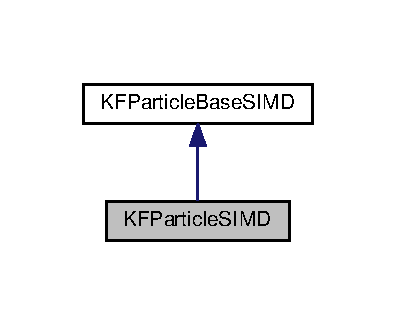
\includegraphics[width=190pt]{classKFParticleSIMD__inherit__graph}
\end{center}
\end{figure}


Collaboration diagram for K\+F\+Particle\+S\+I\+MD\+:
\nopagebreak
\begin{figure}[H]
\begin{center}
\leavevmode
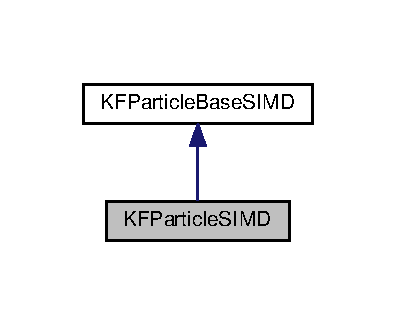
\includegraphics[width=190pt]{classKFParticleSIMD__coll__graph}
\end{center}
\end{figure}
\subsection*{Public Member Functions}
\begin{DoxyCompactItemize}
\item 
void $\ast$ \hyperlink{classKFParticleSIMD_a1c54649173d37330ec67eb02d277a44f}{operator new} (size\+\_\+t size)\hypertarget{classKFParticleSIMD_a1c54649173d37330ec67eb02d277a44f}{}\label{classKFParticleSIMD_a1c54649173d37330ec67eb02d277a44f}

\begin{DoxyCompactList}\small\item\em new operator for allocation of the S\+I\+M\+D-\/alligned dynamic memory allocation \end{DoxyCompactList}\item 
void $\ast$ \hyperlink{classKFParticleSIMD_a50a8252acff97ff2079f9143cfa11760}{operator new\mbox{[}$\,$\mbox{]}} (size\+\_\+t size)\hypertarget{classKFParticleSIMD_a50a8252acff97ff2079f9143cfa11760}{}\label{classKFParticleSIMD_a50a8252acff97ff2079f9143cfa11760}

\begin{DoxyCompactList}\small\item\em new operator for allocation of the S\+I\+M\+D-\/alligned dynamic memory allocation \end{DoxyCompactList}\item 
void $\ast$ \hyperlink{classKFParticleSIMD_a675117630fd9ef18e48d97b2c7980791}{operator new} (size\+\_\+t size, void $\ast$ptr)\hypertarget{classKFParticleSIMD_a675117630fd9ef18e48d97b2c7980791}{}\label{classKFParticleSIMD_a675117630fd9ef18e48d97b2c7980791}

\begin{DoxyCompactList}\small\item\em new operator for allocation of the S\+I\+M\+D-\/alligned dynamic memory allocation \end{DoxyCompactList}\item 
void $\ast$ \hyperlink{classKFParticleSIMD_af0fab5d1fd1e37de0d5598cf24ef776a}{operator new\mbox{[}$\,$\mbox{]}} (size\+\_\+t size, void $\ast$ptr)\hypertarget{classKFParticleSIMD_af0fab5d1fd1e37de0d5598cf24ef776a}{}\label{classKFParticleSIMD_af0fab5d1fd1e37de0d5598cf24ef776a}

\begin{DoxyCompactList}\small\item\em new operator for allocation of the S\+I\+M\+D-\/alligned dynamic memory allocation \end{DoxyCompactList}\item 
void \hyperlink{classKFParticleSIMD_ac9630fbfbe677d322019932503776413}{operator delete} (void $\ast$ptr, size\+\_\+t)\hypertarget{classKFParticleSIMD_ac9630fbfbe677d322019932503776413}{}\label{classKFParticleSIMD_ac9630fbfbe677d322019932503776413}

\begin{DoxyCompactList}\small\item\em delete operator for the S\+I\+M\+D-\/alligned dynamic memory release \end{DoxyCompactList}\item 
void \hyperlink{classKFParticleSIMD_aa06459fe7a2a956252426665a7560d70}{operator delete\mbox{[}$\,$\mbox{]}} (void $\ast$ptr, size\+\_\+t)\hypertarget{classKFParticleSIMD_aa06459fe7a2a956252426665a7560d70}{}\label{classKFParticleSIMD_aa06459fe7a2a956252426665a7560d70}

\begin{DoxyCompactList}\small\item\em delete operator for the S\+I\+M\+D-\/alligned dynamic memory release \end{DoxyCompactList}\item 
\hyperlink{classKFParticleSIMD_a1f82fd50063e4d0f690182f21e6d845e}{K\+F\+Particle\+S\+I\+MD} (const \hyperlink{classKFParticleSIMD}{K\+F\+Particle\+S\+I\+MD} \&d1, const \hyperlink{classKFParticleSIMD}{K\+F\+Particle\+S\+I\+MD} \&d2)
\item 
\hyperlink{classKFParticleSIMD_af71f73034a9c256674afb8442675137c}{K\+F\+Particle\+S\+I\+MD} (const \hyperlink{classKFParticleSIMD}{K\+F\+Particle\+S\+I\+MD} \&d1, const \hyperlink{classKFParticleSIMD}{K\+F\+Particle\+S\+I\+MD} \&d2, const \hyperlink{classKFParticleSIMD}{K\+F\+Particle\+S\+I\+MD} \&d3)
\item 
\hyperlink{classKFParticleSIMD_a3a4d5a4c75ea28e9d993ec9fc7d4fbe8}{K\+F\+Particle\+S\+I\+MD} (const \hyperlink{classKFParticleSIMD}{K\+F\+Particle\+S\+I\+MD} \&d1, const \hyperlink{classKFParticleSIMD}{K\+F\+Particle\+S\+I\+MD} \&d2, const \hyperlink{classKFParticleSIMD}{K\+F\+Particle\+S\+I\+MD} \&d3, const \hyperlink{classKFParticleSIMD}{K\+F\+Particle\+S\+I\+MD} \&d4)
\item 
void \hyperlink{classKFParticleSIMD_ad72c41822502b24af50578767c5fb458}{Create} (const float\+\_\+v Param\mbox{[}$\,$\mbox{]}, const float\+\_\+v Cov\mbox{[}$\,$\mbox{]}, int\+\_\+v Charge, float\+\_\+v mass)
\item 
void \hyperlink{classKFParticleSIMD_a6953ec75b546abb57f1b3fdb035bf337}{Set\+One\+Entry} (int i\+Entry, \hyperlink{classKFParticleSIMD}{K\+F\+Particle\+S\+I\+MD} \&part, int i\+Entry\+Part)
\item 
\hyperlink{classKFParticleSIMD_ab2387938a4518b2a9fbd79b5132d33c8}{K\+F\+Particle\+S\+I\+MD} (const \hyperlink{classKFPTrack}{K\+F\+P\+Track} $\ast$track, Int\+\_\+t P\+ID)
\item 
\hyperlink{classKFParticleSIMD_a9bf7805842574b7e7369ab7b8a3c5cf5}{K\+F\+Particle\+S\+I\+MD} (\hyperlink{classKFPTrack}{K\+F\+P\+Track} $\ast$Track\mbox{[}$\,$\mbox{]}, int N\+Tracks, const Int\+\_\+t $\ast$pdg=nullptr)
\item 
\hyperlink{classKFParticleSIMD_a3c406a7f0392416ab800ed99a7d00a40}{K\+F\+Particle\+S\+I\+MD} (\hyperlink{classKFPTrackVector}{K\+F\+P\+Track\+Vector} \&track, uint\+\_\+v \&index, const int\+\_\+v \&pdg)
\item 
void \hyperlink{classKFParticleSIMD_aafceb974b48b230e42424c95e18a612f}{Create} (\hyperlink{classKFPTrack}{K\+F\+P\+Track} $\ast$Track\mbox{[}$\,$\mbox{]}, int N\+Tracks, const Int\+\_\+t $\ast$pdg=nullptr)
\item 
void \hyperlink{classKFParticleSIMD_ac61bb76736c796c2e47da8ad25b81c27}{Create} (\hyperlink{classKFPTrackVector}{K\+F\+P\+Track\+Vector} \&track, uint\+\_\+v \&index, const int\+\_\+v \&pdg)
\item 
void \hyperlink{classKFParticleSIMD_a0e3c7a0202a62c3c564b22b5d0bfce5e}{Load} (\hyperlink{classKFPTrackVector}{K\+F\+P\+Track\+Vector} \&track, int index, const int\+\_\+v \&pdg)
\item 
void \hyperlink{classKFParticleSIMD_aff00da015d04b572823e5006c3d50eed}{Rotate} ()
\item 
\hyperlink{classKFParticleSIMD_aa9c26d3093382318df37c62badd5567a}{K\+F\+Particle\+S\+I\+MD} (\hyperlink{classKFPTrack}{K\+F\+P\+Track} \&Track, const Int\+\_\+t $\ast$pdg=nullptr)
\item 
\hyperlink{classKFParticleSIMD_aed385589f4efbc4290e69f31f1bb01ec}{K\+F\+Particle\+S\+I\+MD} (\hyperlink{classKFPTrackVector}{K\+F\+P\+Track\+Vector} \&track, int n, const Int\+\_\+t $\ast$pdg=nullptr)
\item 
\hyperlink{classKFParticleSIMD_a6718f90ea49c4cceb12809ea80560856}{K\+F\+Particle\+S\+I\+MD} (\hyperlink{classKFPEmcCluster}{K\+F\+P\+Emc\+Cluster} \&track, uint\+\_\+v \&index, const \hyperlink{classKFParticleSIMD}{K\+F\+Particle\+S\+I\+MD} \&vertex\+Guess)
\item 
\hyperlink{classKFParticleSIMD_abd29270d15669591aa6c763f50b6d63c}{K\+F\+Particle\+S\+I\+MD} (\hyperlink{classKFPEmcCluster}{K\+F\+P\+Emc\+Cluster} \&track, int index, const \hyperlink{classKFParticleSIMD}{K\+F\+Particle\+S\+I\+MD} \&vertex\+Guess)
\item 
void \hyperlink{classKFParticleSIMD_af6012e3bf2cac173cbea677204cdc654}{Create} (\hyperlink{classKFPEmcCluster}{K\+F\+P\+Emc\+Cluster} \&track, uint\+\_\+v \&index, const \hyperlink{classKFParticleSIMD}{K\+F\+Particle\+S\+I\+MD} \&vertex\+Guess)
\item 
void \hyperlink{classKFParticleSIMD_a38255ec3ea343230bc8aa39ebb75a2c6}{Load} (\hyperlink{classKFPEmcCluster}{K\+F\+P\+Emc\+Cluster} \&track, int index, const \hyperlink{classKFParticleSIMD}{K\+F\+Particle\+S\+I\+MD} \&vertex\+Guess)
\item 
\hyperlink{classKFParticleSIMD_aba76dc8326ba159c2e961f9081c7a919}{K\+F\+Particle\+S\+I\+MD} (const \hyperlink{classKFPVertex}{K\+F\+P\+Vertex} \&vertex)
\item 
\hyperlink{classKFParticleSIMD_a43c89c4fa15ede32dc6bdece1b5481cd}{K\+F\+Particle\+S\+I\+MD} (\hyperlink{classKFParticle}{K\+F\+Particle} $\ast$part\mbox{[}$\,$\mbox{]}, int n\+Part=0)
\item 
\hyperlink{classKFParticleSIMD_ac620514cea0df594ee3f0886455b4980}{K\+F\+Particle\+S\+I\+MD} (\hyperlink{classKFParticle}{K\+F\+Particle} \&part)
\item 
Bool\+\_\+t \hyperlink{classKFParticleSIMD_a6b280814d03355ede5f54fd333f65b00}{Get\+At\+Production\+Vertex} () const \hypertarget{classKFParticleSIMD_a6b280814d03355ede5f54fd333f65b00}{}\label{classKFParticleSIMD_a6b280814d03355ede5f54fd333f65b00}

\begin{DoxyCompactList}\small\item\em Returns a flag which shows if the particle is located at the production point. \end{DoxyCompactList}\item 
float\+\_\+v \hyperlink{classKFParticleSIMD_a73e5b4c10ec8ec0f2254da8d7a151e9d}{GetP} () const \hypertarget{classKFParticleSIMD_a73e5b4c10ec8ec0f2254da8d7a151e9d}{}\label{classKFParticleSIMD_a73e5b4c10ec8ec0f2254da8d7a151e9d}

\begin{DoxyCompactList}\small\item\em Returns momentum. \end{DoxyCompactList}\item 
float\+\_\+v \hyperlink{classKFParticleSIMD_afa4110f0c19aeb0e6416a2ff851c121a}{Get\+Pt} () const \hypertarget{classKFParticleSIMD_afa4110f0c19aeb0e6416a2ff851c121a}{}\label{classKFParticleSIMD_afa4110f0c19aeb0e6416a2ff851c121a}

\begin{DoxyCompactList}\small\item\em Returns transverse momentum. \end{DoxyCompactList}\item 
float\+\_\+v \hyperlink{classKFParticleSIMD_a0a034fe797629742f498a57645b2bdd2}{Get\+Eta} () const \hypertarget{classKFParticleSIMD_a0a034fe797629742f498a57645b2bdd2}{}\label{classKFParticleSIMD_a0a034fe797629742f498a57645b2bdd2}

\begin{DoxyCompactList}\small\item\em Returns pseudorapidity. \end{DoxyCompactList}\item 
float\+\_\+v \hyperlink{classKFParticleSIMD_ae03e70e92bba8895c781557f1e16788c}{Get\+Phi} () const \hypertarget{classKFParticleSIMD_ae03e70e92bba8895c781557f1e16788c}{}\label{classKFParticleSIMD_ae03e70e92bba8895c781557f1e16788c}

\begin{DoxyCompactList}\small\item\em Returns the azimuthal angle phi. \end{DoxyCompactList}\item 
float\+\_\+v \hyperlink{classKFParticleSIMD_a8052876b5300379e9dc0cad2cfe4d55a}{Get\+Momentum} () const \hypertarget{classKFParticleSIMD_a8052876b5300379e9dc0cad2cfe4d55a}{}\label{classKFParticleSIMD_a8052876b5300379e9dc0cad2cfe4d55a}

\begin{DoxyCompactList}\small\item\em Returns momentum. \end{DoxyCompactList}\item 
float\+\_\+v \hyperlink{classKFParticleSIMD_a98846262a936a7764d745ecdfbe42946}{Get\+Mass} () const \hypertarget{classKFParticleSIMD_a98846262a936a7764d745ecdfbe42946}{}\label{classKFParticleSIMD_a98846262a936a7764d745ecdfbe42946}

\begin{DoxyCompactList}\small\item\em Returns mass. \end{DoxyCompactList}\item 
float\+\_\+v \hyperlink{classKFParticleSIMD_a509da82165b7684f5036f9bd930ad43e}{Get\+Decay\+Length} () const \hypertarget{classKFParticleSIMD_a509da82165b7684f5036f9bd930ad43e}{}\label{classKFParticleSIMD_a509da82165b7684f5036f9bd930ad43e}

\begin{DoxyCompactList}\small\item\em Returns decay length. \end{DoxyCompactList}\item 
float\+\_\+v \hyperlink{classKFParticleSIMD_aa3ae6056a91fd80d17f54f8e51df8040}{Get\+Decay\+Length\+XY} () const \hypertarget{classKFParticleSIMD_aa3ae6056a91fd80d17f54f8e51df8040}{}\label{classKFParticleSIMD_aa3ae6056a91fd80d17f54f8e51df8040}

\begin{DoxyCompactList}\small\item\em Returns decay length in XY. \end{DoxyCompactList}\item 
float\+\_\+v \hyperlink{classKFParticleSIMD_a375dc8b80e460a60f83baecfbf218aec}{Get\+Life\+Time} () const \hypertarget{classKFParticleSIMD_a375dc8b80e460a60f83baecfbf218aec}{}\label{classKFParticleSIMD_a375dc8b80e460a60f83baecfbf218aec}

\begin{DoxyCompactList}\small\item\em Returns life time ctau \mbox{[}cm\mbox{]}. \end{DoxyCompactList}\item 
float\+\_\+v \hyperlink{classKFParticleSIMD_a7dd8172c4eaf193df4d7897437909234}{GetR} () const \hypertarget{classKFParticleSIMD_a7dd8172c4eaf193df4d7897437909234}{}\label{classKFParticleSIMD_a7dd8172c4eaf193df4d7897437909234}

\begin{DoxyCompactList}\small\item\em Returns distance to the origin of the coordinate system \{0,0,0\}. \end{DoxyCompactList}\item 
float\+\_\+v \hyperlink{classKFParticleSIMD_a2070ffe1acfd297cdbc04e5c8487f5e4}{Get\+Rapidity} () const \hypertarget{classKFParticleSIMD_a2070ffe1acfd297cdbc04e5c8487f5e4}{}\label{classKFParticleSIMD_a2070ffe1acfd297cdbc04e5c8487f5e4}

\begin{DoxyCompactList}\small\item\em Returns rapidity of the particle. \end{DoxyCompactList}\item 
float\+\_\+v \hyperlink{classKFParticleSIMD_a9850f443d65efe8bf2d785423e208472}{Get\+ErrX} () const \hypertarget{classKFParticleSIMD_a9850f443d65efe8bf2d785423e208472}{}\label{classKFParticleSIMD_a9850f443d65efe8bf2d785423e208472}

\begin{DoxyCompactList}\small\item\em Returns the error of X of current position. \end{DoxyCompactList}\item 
float\+\_\+v \hyperlink{classKFParticleSIMD_a77a8d9d475e08abc797281d28d1e42e7}{Get\+ErrY} () const \hypertarget{classKFParticleSIMD_a77a8d9d475e08abc797281d28d1e42e7}{}\label{classKFParticleSIMD_a77a8d9d475e08abc797281d28d1e42e7}

\begin{DoxyCompactList}\small\item\em Returns the error of Y of current position. \end{DoxyCompactList}\item 
float\+\_\+v \hyperlink{classKFParticleSIMD_a781036a835f001708e9a35b221b2bc00}{Get\+ErrZ} () const \hypertarget{classKFParticleSIMD_a781036a835f001708e9a35b221b2bc00}{}\label{classKFParticleSIMD_a781036a835f001708e9a35b221b2bc00}

\begin{DoxyCompactList}\small\item\em Returns the error of Z of current position. \end{DoxyCompactList}\item 
float\+\_\+v \hyperlink{classKFParticleSIMD_af309d5fab0ae5ccefe5f086c11143e04}{Get\+Err\+Px} () const \hypertarget{classKFParticleSIMD_af309d5fab0ae5ccefe5f086c11143e04}{}\label{classKFParticleSIMD_af309d5fab0ae5ccefe5f086c11143e04}

\begin{DoxyCompactList}\small\item\em Returns the error of X-\/compoment of the particle momentum. \end{DoxyCompactList}\item 
float\+\_\+v \hyperlink{classKFParticleSIMD_a9945e5f64ab3104737a83dfa8651da3c}{Get\+Err\+Py} () const \hypertarget{classKFParticleSIMD_a9945e5f64ab3104737a83dfa8651da3c}{}\label{classKFParticleSIMD_a9945e5f64ab3104737a83dfa8651da3c}

\begin{DoxyCompactList}\small\item\em Returns the error of Y-\/compoment of the particle momentum. \end{DoxyCompactList}\item 
float\+\_\+v \hyperlink{classKFParticleSIMD_a8f6fefddc1a1482ed4ac8f087d377f70}{Get\+Err\+Pz} () const \hypertarget{classKFParticleSIMD_a8f6fefddc1a1482ed4ac8f087d377f70}{}\label{classKFParticleSIMD_a8f6fefddc1a1482ed4ac8f087d377f70}

\begin{DoxyCompactList}\small\item\em Returns the error of Z-\/compoment of the particle momentum. \end{DoxyCompactList}\item 
float\+\_\+v \hyperlink{classKFParticleSIMD_aeb88dc2944d959f9579398135fedc24e}{Get\+ErrE} () const \hypertarget{classKFParticleSIMD_aeb88dc2944d959f9579398135fedc24e}{}\label{classKFParticleSIMD_aeb88dc2944d959f9579398135fedc24e}

\begin{DoxyCompactList}\small\item\em Returns the error of energy. \end{DoxyCompactList}\item 
float\+\_\+v \hyperlink{classKFParticleSIMD_a628e6f0aa1fd791274b4e3b94ff0404a}{Get\+ErrS} () const \hypertarget{classKFParticleSIMD_a628e6f0aa1fd791274b4e3b94ff0404a}{}\label{classKFParticleSIMD_a628e6f0aa1fd791274b4e3b94ff0404a}

\begin{DoxyCompactList}\small\item\em Returns the error of decay length / momentum. \end{DoxyCompactList}\item 
float\+\_\+v \hyperlink{classKFParticleSIMD_a9531e40fb9ae49f4fc7f2344a2977072}{Get\+ErrP} () const \hypertarget{classKFParticleSIMD_a9531e40fb9ae49f4fc7f2344a2977072}{}\label{classKFParticleSIMD_a9531e40fb9ae49f4fc7f2344a2977072}

\begin{DoxyCompactList}\small\item\em Returns the error of momentum. \end{DoxyCompactList}\item 
float\+\_\+v \hyperlink{classKFParticleSIMD_a398ff53645050d8527c3c77781f9be0e}{Get\+Err\+Pt} () const \hypertarget{classKFParticleSIMD_a398ff53645050d8527c3c77781f9be0e}{}\label{classKFParticleSIMD_a398ff53645050d8527c3c77781f9be0e}

\begin{DoxyCompactList}\small\item\em Returns the error of transverse momentum. \end{DoxyCompactList}\item 
float\+\_\+v \hyperlink{classKFParticleSIMD_ad9ce07062930794c651c1c14b9a92c8b}{Get\+Err\+Eta} () const \hypertarget{classKFParticleSIMD_ad9ce07062930794c651c1c14b9a92c8b}{}\label{classKFParticleSIMD_ad9ce07062930794c651c1c14b9a92c8b}

\begin{DoxyCompactList}\small\item\em Returns the error of pseudorapidity. \end{DoxyCompactList}\item 
float\+\_\+v \hyperlink{classKFParticleSIMD_a38af99b90699ed86707db793a4c24a4d}{Get\+Err\+Phi} () const \hypertarget{classKFParticleSIMD_a38af99b90699ed86707db793a4c24a4d}{}\label{classKFParticleSIMD_a38af99b90699ed86707db793a4c24a4d}

\begin{DoxyCompactList}\small\item\em Returns the error of the azimuthal angle phi. \end{DoxyCompactList}\item 
float\+\_\+v \hyperlink{classKFParticleSIMD_a7bad6a41dbcbe77641c6d35743cf7f75}{Get\+Err\+Momentum} () const \hypertarget{classKFParticleSIMD_a7bad6a41dbcbe77641c6d35743cf7f75}{}\label{classKFParticleSIMD_a7bad6a41dbcbe77641c6d35743cf7f75}

\begin{DoxyCompactList}\small\item\em Returns the error of momentum. \end{DoxyCompactList}\item 
float\+\_\+v \hyperlink{classKFParticleSIMD_a73928ff05b0df6b1cb038d224eabe4cd}{Get\+Err\+Mass} () const \hypertarget{classKFParticleSIMD_a73928ff05b0df6b1cb038d224eabe4cd}{}\label{classKFParticleSIMD_a73928ff05b0df6b1cb038d224eabe4cd}

\begin{DoxyCompactList}\small\item\em Returns the error of mass. \end{DoxyCompactList}\item 
float\+\_\+v \hyperlink{classKFParticleSIMD_a355cd7aafcef1798409d9c1e253755a4}{Get\+Err\+Decay\+Length} () const \hypertarget{classKFParticleSIMD_a355cd7aafcef1798409d9c1e253755a4}{}\label{classKFParticleSIMD_a355cd7aafcef1798409d9c1e253755a4}

\begin{DoxyCompactList}\small\item\em Returns the error of decay length. \end{DoxyCompactList}\item 
float\+\_\+v \hyperlink{classKFParticleSIMD_a1cb105a0315a24031360346160f48c5f}{Get\+Err\+Decay\+Length\+XY} () const \hypertarget{classKFParticleSIMD_a1cb105a0315a24031360346160f48c5f}{}\label{classKFParticleSIMD_a1cb105a0315a24031360346160f48c5f}

\begin{DoxyCompactList}\small\item\em Returns the error of decay length in XY. \end{DoxyCompactList}\item 
float\+\_\+v \hyperlink{classKFParticleSIMD_a9756232862db86c5c45bdbe9744b49f1}{Get\+Err\+Life\+Time} () const \hypertarget{classKFParticleSIMD_a9756232862db86c5c45bdbe9744b49f1}{}\label{classKFParticleSIMD_a9756232862db86c5c45bdbe9744b49f1}

\begin{DoxyCompactList}\small\item\em Returns the error of life time. \end{DoxyCompactList}\item 
float\+\_\+v \hyperlink{classKFParticleSIMD_af72ee39cb2f92477b14a8c748746692d}{Get\+ErrR} () const \hypertarget{classKFParticleSIMD_af72ee39cb2f92477b14a8c748746692d}{}\label{classKFParticleSIMD_af72ee39cb2f92477b14a8c748746692d}

\begin{DoxyCompactList}\small\item\em Returns the error of distance to the origin of the coordinate system \{0,0,0\}. \end{DoxyCompactList}\item 
float\+\_\+v $\ast$ \hyperlink{classKFParticleSIMD_a27d7e843526677a4a1a0b755f7fb5d65}{Parameters} ()\hypertarget{classKFParticleSIMD_a27d7e843526677a4a1a0b755f7fb5d65}{}\label{classKFParticleSIMD_a27d7e843526677a4a1a0b755f7fb5d65}

\begin{DoxyCompactList}\small\item\em Returns pointer to the parameters fP. \end{DoxyCompactList}\item 
float\+\_\+v $\ast$ \hyperlink{classKFParticleSIMD_aaa2f81f07799d2d9beaede2e7864a1a9}{Covariance\+Matrix} ()\hypertarget{classKFParticleSIMD_aaa2f81f07799d2d9beaede2e7864a1a9}{}\label{classKFParticleSIMD_aaa2f81f07799d2d9beaede2e7864a1a9}

\begin{DoxyCompactList}\small\item\em Returns pointer to the covariance matrix fC. \end{DoxyCompactList}\item 
void \hyperlink{classKFParticleSIMD_abee0e1ab2c3a9a40f6618a20fb58f664}{Get\+K\+F\+Particle} (\hyperlink{classKFParticle}{K\+F\+Particle} \&Part, int i\+Part=0)
\item 
void \hyperlink{classKFParticleSIMD_a52e83afab8f9b1d755ae0e1a4e9fdde7}{Get\+K\+F\+Particle} (\hyperlink{classKFParticle}{K\+F\+Particle} $\ast$Part, int n\+Part=0)
\item 
void \hyperlink{classKFParticleSIMD_afd134dee761fd11c9f22c05a0a5262ca}{Add\+Daughter} (const \hyperlink{classKFParticleSIMD}{K\+F\+Particle\+S\+I\+MD} \&Daughter)
\item 
void \hyperlink{classKFParticleSIMD_a7a8fccbeb58437f20fee5cb68e6f1259}{operator+=} (const \hyperlink{classKFParticleSIMD}{K\+F\+Particle\+S\+I\+MD} \&Daughter)
\item 
void \hyperlink{classKFParticleSIMD_a54d024bbcfef5d7f99e1ed7b45973221}{Construct} (const \hyperlink{classKFParticleSIMD}{K\+F\+Particle\+S\+I\+MD} $\ast$v\+Daughters\mbox{[}$\,$\mbox{]}, int n\+Daughters, const \hyperlink{classKFParticleSIMD}{K\+F\+Particle\+S\+I\+MD} $\ast$Prod\+Vtx=nullptr, Float\+\_\+t Mass=-\/1)
\item 
void \hyperlink{classKFParticleSIMD_ac4c896519f2acc22953b5b943bc8e08a}{Transport\+To\+Point} (const float\+\_\+v xyz\mbox{[}$\,$\mbox{]})
\item 
void \hyperlink{classKFParticleSIMD_a75ee554571b29ef90452c2834bebdb1a}{Transport\+To\+Particle} (const \hyperlink{classKFParticleSIMD}{K\+F\+Particle\+S\+I\+MD} \&p)
\item 
float\+\_\+v \hyperlink{classKFParticleSIMD_adf768a35209bb2f98adf8a12e21a09d4}{Get\+D\+Sto\+Point} (const float\+\_\+v xyz\mbox{[}3\mbox{]}, float\+\_\+v dsdr\mbox{[}6\mbox{]}) const 
\item 
void \hyperlink{classKFParticleSIMD_ad8379c5666e84d5c1de7dd1428234744}{Get\+D\+Sto\+Particle} (const \hyperlink{classKFParticleBaseSIMD}{K\+F\+Particle\+Base\+S\+I\+MD} \&p, float\+\_\+v dS\mbox{[}2\mbox{]}, float\+\_\+v dsdr\mbox{[}4\mbox{]}\mbox{[}6\mbox{]}) const 
\item 
void \hyperlink{classKFParticleSIMD_ac4bcc9cda90e1454fd9ab18bfd7bd012}{Get\+D\+Sto\+Particle\+Fast} (const \hyperlink{classKFParticleBaseSIMD}{K\+F\+Particle\+Base\+S\+I\+MD} \&p, float\+\_\+v dS\mbox{[}2\mbox{]}) const 
\item 
float\+\_\+m \hyperlink{classKFParticleSIMD_a874d6387e88fce6fe69d7a6a811a377f}{Get\+Distance\+From\+Vertex\+XY} (const float\+\_\+v vtx\mbox{[}$\,$\mbox{]}, float\+\_\+v \&val, float\+\_\+v \&err) const 
\item 
float\+\_\+m \hyperlink{classKFParticleSIMD_a2ebfe06b454da6d2b7c5d0bfef26e9ca}{Get\+Distance\+From\+Vertex\+XY} (const float\+\_\+v vtx\mbox{[}$\,$\mbox{]}, const float\+\_\+v Cv\mbox{[}$\,$\mbox{]}, float\+\_\+v \&val, float\+\_\+v \&err) const 
\item 
float\+\_\+m \hyperlink{classKFParticleSIMD_a20395d1d794abd0e0922c7dca48950db}{Get\+Distance\+From\+Vertex\+XY} (const \hyperlink{classKFParticleSIMD}{K\+F\+Particle\+S\+I\+MD} \&Vtx, float\+\_\+v \&val, float\+\_\+v \&err) const 
\item 
float\+\_\+v \hyperlink{classKFParticleSIMD_a9d5224c105404e7cd293d29823de1094}{Get\+Distance\+From\+Vertex\+XY} (const float\+\_\+v vtx\mbox{[}$\,$\mbox{]}) const 
\item 
float\+\_\+v \hyperlink{classKFParticleSIMD_a1fa77112f03433e799068e573c2a07d6}{Get\+Distance\+From\+Vertex\+XY} (const \hyperlink{classKFParticleSIMD}{K\+F\+Particle\+S\+I\+MD} \&Vtx) const 
\item 
float\+\_\+v \hyperlink{classKFParticleSIMD_aa8fb673d2b680ca33297a1e401aa7208}{Get\+Distance\+From\+Particle\+XY} (const \hyperlink{classKFParticleSIMD}{K\+F\+Particle\+S\+I\+MD} \&p) const 
\item 
float\+\_\+v \hyperlink{classKFParticleSIMD_aa636c8a09e8e53b2393eb7e4e02a7127}{Get\+Deviation\+From\+Vertex\+XY} (const float\+\_\+v v\mbox{[}$\,$\mbox{]}, const float\+\_\+v Cv\mbox{[}$\,$\mbox{]}=nullptr) const 
\item 
float\+\_\+v \hyperlink{classKFParticleSIMD_a1b524c1e7e92bcb25417e072198676da}{Get\+Deviation\+From\+Vertex\+XY} (const \hyperlink{classKFParticleSIMD}{K\+F\+Particle\+S\+I\+MD} \&Vtx) const 
\item 
float\+\_\+v \hyperlink{classKFParticleSIMD_aeef9436d096312a52ff8d9a2e691f115}{Get\+Deviation\+From\+Particle\+XY} (const \hyperlink{classKFParticleSIMD}{K\+F\+Particle\+S\+I\+MD} \&p) const 
\item 
float\+\_\+v \hyperlink{classKFParticleSIMD_a742d47505d1051ecf081040ac15c9798}{Get\+Angle} (const \hyperlink{classKFParticleSIMD}{K\+F\+Particle\+S\+I\+MD} \&p) const 
\item 
float\+\_\+v \hyperlink{classKFParticleSIMD_a485a5cc06021dbc62322c2cb7a706251}{Get\+Angle\+XY} (const \hyperlink{classKFParticleSIMD}{K\+F\+Particle\+S\+I\+MD} \&p) const 
\item 
float\+\_\+v \hyperlink{classKFParticleSIMD_acf26f94fdfb68a8983b0b601ae86a3ff}{Get\+Angle\+RZ} (const \hyperlink{classKFParticleSIMD}{K\+F\+Particle\+S\+I\+MD} \&p) const 
\item 
float\+\_\+v \hyperlink{classKFParticleSIMD_a97da667746e38c615d6652efcdb2d378}{Get\+Pseudo\+Proper\+Decay\+Time} (const \hyperlink{classKFParticleSIMD}{K\+F\+Particle\+S\+I\+MD} \&prim\+Vertex, const float\+\_\+v \&mass, float\+\_\+v $\ast$time\+Err2=nullptr) const 
\item 
void \hyperlink{classKFParticleSIMD_aa690422efc2940cb8b38280b592831d4}{Get\+Field\+Value} (const float\+\_\+v xyz\mbox{[}$\,$\mbox{]}, float\+\_\+v B\mbox{[}$\,$\mbox{]}) const 
\item 
void \hyperlink{classKFParticleSIMD_a30f4af6707803e1f959559db63fb620a}{Transport} (float\+\_\+v dS, const float\+\_\+v $\ast$dsdr, float\+\_\+v P\mbox{[}$\,$\mbox{]}, float\+\_\+v C\mbox{[}$\,$\mbox{]}, float\+\_\+v $\ast$dsdr1=nullptr, float\+\_\+v $\ast$F=nullptr, float\+\_\+v $\ast$F1=nullptr) const 
\item 
void \hyperlink{classKFParticleSIMD_a7fffef3f8325407951238797bfb3c8fc}{Transport\+Fast} (float\+\_\+v dS, float\+\_\+v P\mbox{[}$\,$\mbox{]}) const 
\end{DoxyCompactItemize}
\subsection*{Additional Inherited Members}


\subsection{Detailed Description}
The main vectorised class of KF Particle pacakge, describes particle objects. 

\begin{DoxyAuthor}{Author}
M.\+Zyzak 
\end{DoxyAuthor}
\begin{DoxyDate}{Date}
05.\+02.\+2019 
\end{DoxyDate}
\begin{DoxyVersion}{Version}
1.\+0
\end{DoxyVersion}
Vectorised version of the KF Particle class, describes particle objects. The particle is described with the state vector \{ X, Y, Z, Px, Py, Pz, E \} and the corresponding covariance matrix. It contains functionality to create particle-\/object from track, to construct short-\/lived particles from other tracks or particles. The mathematics is based on the Kalman filter method. It also allows to subtract particles from the already constructed object, to transport partices, get parameters together with their erros, get distance to other particles and vertices, get deviations from them in terms of errors, etc. 

\subsection{Constructor \& Destructor Documentation}
\index{K\+F\+Particle\+S\+I\+MD@{K\+F\+Particle\+S\+I\+MD}!K\+F\+Particle\+S\+I\+MD@{K\+F\+Particle\+S\+I\+MD}}
\index{K\+F\+Particle\+S\+I\+MD@{K\+F\+Particle\+S\+I\+MD}!K\+F\+Particle\+S\+I\+MD@{K\+F\+Particle\+S\+I\+MD}}
\subsubsection[{\texorpdfstring{K\+F\+Particle\+S\+I\+M\+D(const K\+F\+Particle\+S\+I\+M\+D \&d1, const K\+F\+Particle\+S\+I\+M\+D \&d2)}{KFParticleSIMD(const KFParticleSIMD &d1, const KFParticleSIMD &d2)}}]{\setlength{\rightskip}{0pt plus 5cm}K\+F\+Particle\+S\+I\+M\+D\+::\+K\+F\+Particle\+S\+I\+MD (
\begin{DoxyParamCaption}
\item[{const {\bf K\+F\+Particle\+S\+I\+MD} \&}]{d1, }
\item[{const {\bf K\+F\+Particle\+S\+I\+MD} \&}]{d2}
\end{DoxyParamCaption}
)}\hypertarget{classKFParticleSIMD_a1f82fd50063e4d0f690182f21e6d845e}{}\label{classKFParticleSIMD_a1f82fd50063e4d0f690182f21e6d845e}
Constructs a particle from two input daughter particles 
\begin{DoxyParams}[1]{Parameters}
\mbox{\tt in}  & {\em d1} & -\/ the first daughter particle \\
\hline
\mbox{\tt in}  & {\em d2} & -\/ the second daughter particle\\
\hline
\end{DoxyParams}
\index{K\+F\+Particle\+S\+I\+MD@{K\+F\+Particle\+S\+I\+MD}!K\+F\+Particle\+S\+I\+MD@{K\+F\+Particle\+S\+I\+MD}}
\index{K\+F\+Particle\+S\+I\+MD@{K\+F\+Particle\+S\+I\+MD}!K\+F\+Particle\+S\+I\+MD@{K\+F\+Particle\+S\+I\+MD}}
\subsubsection[{\texorpdfstring{K\+F\+Particle\+S\+I\+M\+D(const K\+F\+Particle\+S\+I\+M\+D \&d1, const K\+F\+Particle\+S\+I\+M\+D \&d2, const K\+F\+Particle\+S\+I\+M\+D \&d3)}{KFParticleSIMD(const KFParticleSIMD &d1, const KFParticleSIMD &d2, const KFParticleSIMD &d3)}}]{\setlength{\rightskip}{0pt plus 5cm}K\+F\+Particle\+S\+I\+M\+D\+::\+K\+F\+Particle\+S\+I\+MD (
\begin{DoxyParamCaption}
\item[{const {\bf K\+F\+Particle\+S\+I\+MD} \&}]{d1, }
\item[{const {\bf K\+F\+Particle\+S\+I\+MD} \&}]{d2, }
\item[{const {\bf K\+F\+Particle\+S\+I\+MD} \&}]{d3}
\end{DoxyParamCaption}
)\hspace{0.3cm}{\ttfamily [inline]}}\hypertarget{classKFParticleSIMD_af71f73034a9c256674afb8442675137c}{}\label{classKFParticleSIMD_af71f73034a9c256674afb8442675137c}
Constructs a particle from three input daughter particles 
\begin{DoxyParams}[1]{Parameters}
\mbox{\tt in}  & {\em d1} & -\/ the first daughter particle \\
\hline
\mbox{\tt in}  & {\em d2} & -\/ the second daughter particle \\
\hline
\mbox{\tt in}  & {\em d3} & -\/ the third daughter particle\\
\hline
\end{DoxyParams}
\index{K\+F\+Particle\+S\+I\+MD@{K\+F\+Particle\+S\+I\+MD}!K\+F\+Particle\+S\+I\+MD@{K\+F\+Particle\+S\+I\+MD}}
\index{K\+F\+Particle\+S\+I\+MD@{K\+F\+Particle\+S\+I\+MD}!K\+F\+Particle\+S\+I\+MD@{K\+F\+Particle\+S\+I\+MD}}
\subsubsection[{\texorpdfstring{K\+F\+Particle\+S\+I\+M\+D(const K\+F\+Particle\+S\+I\+M\+D \&d1, const K\+F\+Particle\+S\+I\+M\+D \&d2, const K\+F\+Particle\+S\+I\+M\+D \&d3, const K\+F\+Particle\+S\+I\+M\+D \&d4)}{KFParticleSIMD(const KFParticleSIMD &d1, const KFParticleSIMD &d2, const KFParticleSIMD &d3, const KFParticleSIMD &d4)}}]{\setlength{\rightskip}{0pt plus 5cm}K\+F\+Particle\+S\+I\+M\+D\+::\+K\+F\+Particle\+S\+I\+MD (
\begin{DoxyParamCaption}
\item[{const {\bf K\+F\+Particle\+S\+I\+MD} \&}]{d1, }
\item[{const {\bf K\+F\+Particle\+S\+I\+MD} \&}]{d2, }
\item[{const {\bf K\+F\+Particle\+S\+I\+MD} \&}]{d3, }
\item[{const {\bf K\+F\+Particle\+S\+I\+MD} \&}]{d4}
\end{DoxyParamCaption}
)\hspace{0.3cm}{\ttfamily [inline]}}\hypertarget{classKFParticleSIMD_a3a4d5a4c75ea28e9d993ec9fc7d4fbe8}{}\label{classKFParticleSIMD_a3a4d5a4c75ea28e9d993ec9fc7d4fbe8}
Constructs a particle from four input daughter particles 
\begin{DoxyParams}[1]{Parameters}
\mbox{\tt in}  & {\em d1} & -\/ the first daughter particle \\
\hline
\mbox{\tt in}  & {\em d2} & -\/ the second daughter particle \\
\hline
\mbox{\tt in}  & {\em d3} & -\/ the third daughter particle \\
\hline
\mbox{\tt in}  & {\em d4} & -\/ the fourth daughter particle\\
\hline
\end{DoxyParams}
\index{K\+F\+Particle\+S\+I\+MD@{K\+F\+Particle\+S\+I\+MD}!K\+F\+Particle\+S\+I\+MD@{K\+F\+Particle\+S\+I\+MD}}
\index{K\+F\+Particle\+S\+I\+MD@{K\+F\+Particle\+S\+I\+MD}!K\+F\+Particle\+S\+I\+MD@{K\+F\+Particle\+S\+I\+MD}}
\subsubsection[{\texorpdfstring{K\+F\+Particle\+S\+I\+M\+D(const K\+F\+P\+Track $\ast$track, Int\+\_\+t P\+I\+D)}{KFParticleSIMD(const KFPTrack *track, Int_t PID)}}]{\setlength{\rightskip}{0pt plus 5cm}K\+F\+Particle\+S\+I\+M\+D\+::\+K\+F\+Particle\+S\+I\+MD (
\begin{DoxyParamCaption}
\item[{const {\bf K\+F\+P\+Track} $\ast$}]{track, }
\item[{Int\+\_\+t}]{P\+ID}
\end{DoxyParamCaption}
)}\hypertarget{classKFParticleSIMD_ab2387938a4518b2a9fbd79b5132d33c8}{}\label{classKFParticleSIMD_ab2387938a4518b2a9fbd79b5132d33c8}
Constructor of the particle from an array of tracks. 
\begin{DoxyParams}[1]{Parameters}
\mbox{\tt in}  & {\em track} & -\/ pointer to the array of n=float\+\_\+v\+Len tracks \\
\hline
\mbox{\tt in}  & {\em P\+ID} & -\/ the P\+ID hypothesis common for all elements of the S\+I\+MD vector\\
\hline
\end{DoxyParams}
\index{K\+F\+Particle\+S\+I\+MD@{K\+F\+Particle\+S\+I\+MD}!K\+F\+Particle\+S\+I\+MD@{K\+F\+Particle\+S\+I\+MD}}
\index{K\+F\+Particle\+S\+I\+MD@{K\+F\+Particle\+S\+I\+MD}!K\+F\+Particle\+S\+I\+MD@{K\+F\+Particle\+S\+I\+MD}}
\subsubsection[{\texorpdfstring{K\+F\+Particle\+S\+I\+M\+D(\+K\+F\+P\+Track $\ast$\+Track[], int N\+Tracks, const Int\+\_\+t $\ast$pdg=nullptr)}{KFParticleSIMD(KFPTrack *Track[], int NTracks, const Int_t *pdg=nullptr)}}]{\setlength{\rightskip}{0pt plus 5cm}K\+F\+Particle\+S\+I\+M\+D\+::\+K\+F\+Particle\+S\+I\+MD (
\begin{DoxyParamCaption}
\item[{{\bf K\+F\+P\+Track} $\ast$}]{Track\mbox{[}$\,$\mbox{]}, }
\item[{int}]{N\+Tracks, }
\item[{const Int\+\_\+t $\ast$}]{pdg = {\ttfamily nullptr}}
\end{DoxyParamCaption}
)}\hypertarget{classKFParticleSIMD_a9bf7805842574b7e7369ab7b8a3c5cf5}{}\label{classKFParticleSIMD_a9bf7805842574b7e7369ab7b8a3c5cf5}
Constructor of the particle from an array tracks. 
\begin{DoxyParams}[1]{Parameters}
\mbox{\tt in}  & {\em Track} & -\/ an array of pointers to tracks in the \hyperlink{classKFPTrack}{K\+F\+P\+Track} format \\
\hline
\mbox{\tt in}  & {\em N\+Tracks} & -\/ number of tracks in the arry \\
\hline
\mbox{\tt in}  & {\em pdg} & -\/ pointer to the pdg hypothesis common for all elements of the S\+I\+MD vector\\
\hline
\end{DoxyParams}
\index{K\+F\+Particle\+S\+I\+MD@{K\+F\+Particle\+S\+I\+MD}!K\+F\+Particle\+S\+I\+MD@{K\+F\+Particle\+S\+I\+MD}}
\index{K\+F\+Particle\+S\+I\+MD@{K\+F\+Particle\+S\+I\+MD}!K\+F\+Particle\+S\+I\+MD@{K\+F\+Particle\+S\+I\+MD}}
\subsubsection[{\texorpdfstring{K\+F\+Particle\+S\+I\+M\+D(\+K\+F\+P\+Track\+Vector \&track, uint\+\_\+v \&index, const int\+\_\+v \&pdg)}{KFParticleSIMD(KFPTrackVector &track, uint_v &index, const int_v &pdg)}}]{\setlength{\rightskip}{0pt plus 5cm}K\+F\+Particle\+S\+I\+M\+D\+::\+K\+F\+Particle\+S\+I\+MD (
\begin{DoxyParamCaption}
\item[{{\bf K\+F\+P\+Track\+Vector} \&}]{track, }
\item[{uint\+\_\+v \&}]{index, }
\item[{const int\+\_\+v \&}]{pdg}
\end{DoxyParamCaption}
)}\hypertarget{classKFParticleSIMD_a3c406a7f0392416ab800ed99a7d00a40}{}\label{classKFParticleSIMD_a3c406a7f0392416ab800ed99a7d00a40}
Constructor of the particle from a set of tracks with random indices \char`\"{}index\char`\"{} stored in the \hyperlink{classKFPTrackVector}{K\+F\+P\+Track\+Vector} format. 
\begin{DoxyParams}[1]{Parameters}
\mbox{\tt in}  & {\em track} & -\/ an array with tracks in the \hyperlink{classKFPTrackVector}{K\+F\+P\+Track\+Vector} format \\
\hline
\mbox{\tt in}  & {\em index} & -\/ indices of the tracks to be converted to the \hyperlink{classKFParticleSIMD}{K\+F\+Particle\+S\+I\+MD} object \\
\hline
\mbox{\tt in}  & {\em pdg} & -\/ a S\+I\+MD vector with an individual pdg hypothesis for each element\\
\hline
\end{DoxyParams}
\index{K\+F\+Particle\+S\+I\+MD@{K\+F\+Particle\+S\+I\+MD}!K\+F\+Particle\+S\+I\+MD@{K\+F\+Particle\+S\+I\+MD}}
\index{K\+F\+Particle\+S\+I\+MD@{K\+F\+Particle\+S\+I\+MD}!K\+F\+Particle\+S\+I\+MD@{K\+F\+Particle\+S\+I\+MD}}
\subsubsection[{\texorpdfstring{K\+F\+Particle\+S\+I\+M\+D(\+K\+F\+P\+Track \&\+Track, const Int\+\_\+t $\ast$pdg=nullptr)}{KFParticleSIMD(KFPTrack &Track, const Int_t *pdg=nullptr)}}]{\setlength{\rightskip}{0pt plus 5cm}K\+F\+Particle\+S\+I\+M\+D\+::\+K\+F\+Particle\+S\+I\+MD (
\begin{DoxyParamCaption}
\item[{{\bf K\+F\+P\+Track} \&}]{Track, }
\item[{const Int\+\_\+t $\ast$}]{pdg = {\ttfamily nullptr}}
\end{DoxyParamCaption}
)}\hypertarget{classKFParticleSIMD_aa9c26d3093382318df37c62badd5567a}{}\label{classKFParticleSIMD_aa9c26d3093382318df37c62badd5567a}
Constructor of the particle from a single track. The same track is put to each element of the S\+I\+MD vector. 
\begin{DoxyParams}[1]{Parameters}
\mbox{\tt in}  & {\em Track} & -\/ track in the \hyperlink{classKFPTrack}{K\+F\+P\+Track} format \\
\hline
\mbox{\tt in}  & {\em P\+ID} & -\/ the P\+ID hypothesis common for all elements of the S\+I\+MD vector\\
\hline
\end{DoxyParams}
\index{K\+F\+Particle\+S\+I\+MD@{K\+F\+Particle\+S\+I\+MD}!K\+F\+Particle\+S\+I\+MD@{K\+F\+Particle\+S\+I\+MD}}
\index{K\+F\+Particle\+S\+I\+MD@{K\+F\+Particle\+S\+I\+MD}!K\+F\+Particle\+S\+I\+MD@{K\+F\+Particle\+S\+I\+MD}}
\subsubsection[{\texorpdfstring{K\+F\+Particle\+S\+I\+M\+D(\+K\+F\+P\+Track\+Vector \&track, int n, const Int\+\_\+t $\ast$pdg=nullptr)}{KFParticleSIMD(KFPTrackVector &track, int n, const Int_t *pdg=nullptr)}}]{\setlength{\rightskip}{0pt plus 5cm}K\+F\+Particle\+S\+I\+M\+D\+::\+K\+F\+Particle\+S\+I\+MD (
\begin{DoxyParamCaption}
\item[{{\bf K\+F\+P\+Track\+Vector} \&}]{track, }
\item[{int}]{n, }
\item[{const Int\+\_\+t $\ast$}]{pdg = {\ttfamily nullptr}}
\end{DoxyParamCaption}
)}\hypertarget{classKFParticleSIMD_aed385589f4efbc4290e69f31f1bb01ec}{}\label{classKFParticleSIMD_aed385589f4efbc4290e69f31f1bb01ec}
Constructor of the particle from a single track with index \char`\"{}n\char`\"{} stored in the \hyperlink{classKFPTrackVector}{K\+F\+P\+Track\+Vector} format. The same track is put to each element of the S\+I\+MD vector. 
\begin{DoxyParams}[1]{Parameters}
\mbox{\tt in}  & {\em track} & -\/ an array with tracks in the \hyperlink{classKFPTrackVector}{K\+F\+P\+Track\+Vector} format \\
\hline
\mbox{\tt in}  & {\em n} & -\/ index of the track to be used \\
\hline
\mbox{\tt in}  & {\em pdg} & -\/ pointer to the pdg hypothesis\\
\hline
\end{DoxyParams}
\index{K\+F\+Particle\+S\+I\+MD@{K\+F\+Particle\+S\+I\+MD}!K\+F\+Particle\+S\+I\+MD@{K\+F\+Particle\+S\+I\+MD}}
\index{K\+F\+Particle\+S\+I\+MD@{K\+F\+Particle\+S\+I\+MD}!K\+F\+Particle\+S\+I\+MD@{K\+F\+Particle\+S\+I\+MD}}
\subsubsection[{\texorpdfstring{K\+F\+Particle\+S\+I\+M\+D(\+K\+F\+P\+Emc\+Cluster \&track, uint\+\_\+v \&index, const K\+F\+Particle\+S\+I\+M\+D \&vertex\+Guess)}{KFParticleSIMD(KFPEmcCluster &track, uint_v &index, const KFParticleSIMD &vertexGuess)}}]{\setlength{\rightskip}{0pt plus 5cm}K\+F\+Particle\+S\+I\+M\+D\+::\+K\+F\+Particle\+S\+I\+MD (
\begin{DoxyParamCaption}
\item[{{\bf K\+F\+P\+Emc\+Cluster} \&}]{track, }
\item[{uint\+\_\+v \&}]{index, }
\item[{const {\bf K\+F\+Particle\+S\+I\+MD} \&}]{vertex\+Guess}
\end{DoxyParamCaption}
)}\hypertarget{classKFParticleSIMD_a6718f90ea49c4cceb12809ea80560856}{}\label{classKFParticleSIMD_a6718f90ea49c4cceb12809ea80560856}
Constructor of gamma particles from a set of clusters of the electromagnetic calorimeter (E\+MC) with random indices \char`\"{}index\char`\"{}. The vertex hypothesis should be provided for the estimation of the momentum. 
\begin{DoxyParams}[1]{Parameters}
\mbox{\tt in}  & {\em track} & -\/ an array of E\+MC clusters \\
\hline
\mbox{\tt in}  & {\em index} & -\/ indices of the clusters to be converted to the \hyperlink{classKFParticleSIMD}{K\+F\+Particle\+S\+I\+MD} object \\
\hline
\mbox{\tt in}  & {\em vertex\+Guess} & -\/ vertex guess for estimation of the momentum of created gamma particles\\
\hline
\end{DoxyParams}
\index{K\+F\+Particle\+S\+I\+MD@{K\+F\+Particle\+S\+I\+MD}!K\+F\+Particle\+S\+I\+MD@{K\+F\+Particle\+S\+I\+MD}}
\index{K\+F\+Particle\+S\+I\+MD@{K\+F\+Particle\+S\+I\+MD}!K\+F\+Particle\+S\+I\+MD@{K\+F\+Particle\+S\+I\+MD}}
\subsubsection[{\texorpdfstring{K\+F\+Particle\+S\+I\+M\+D(\+K\+F\+P\+Emc\+Cluster \&track, int index, const K\+F\+Particle\+S\+I\+M\+D \&vertex\+Guess)}{KFParticleSIMD(KFPEmcCluster &track, int index, const KFParticleSIMD &vertexGuess)}}]{\setlength{\rightskip}{0pt plus 5cm}K\+F\+Particle\+S\+I\+M\+D\+::\+K\+F\+Particle\+S\+I\+MD (
\begin{DoxyParamCaption}
\item[{{\bf K\+F\+P\+Emc\+Cluster} \&}]{track, }
\item[{int}]{index, }
\item[{const {\bf K\+F\+Particle\+S\+I\+MD} \&}]{vertex\+Guess}
\end{DoxyParamCaption}
)}\hypertarget{classKFParticleSIMD_abd29270d15669591aa6c763f50b6d63c}{}\label{classKFParticleSIMD_abd29270d15669591aa6c763f50b6d63c}
Constructr gamma particles from a set of consequetive clusters of the electromagnetic calorimeter (E\+MC) starting from the index \char`\"{}index\char`\"{}. The vertex hypothesis should be provided for the estimation of the momentum. 
\begin{DoxyParams}[1]{Parameters}
\mbox{\tt in}  & {\em track} & -\/ an array with tracks in the \hyperlink{classKFPTrackVector}{K\+F\+P\+Track\+Vector} format \\
\hline
\mbox{\tt in}  & {\em index} & -\/ index of the first E\+MC cluster \\
\hline
\mbox{\tt in}  & {\em vertex\+Guess} & -\/ vertex guess for estimation of the momentum of created gamma particles\\
\hline
\end{DoxyParams}
\index{K\+F\+Particle\+S\+I\+MD@{K\+F\+Particle\+S\+I\+MD}!K\+F\+Particle\+S\+I\+MD@{K\+F\+Particle\+S\+I\+MD}}
\index{K\+F\+Particle\+S\+I\+MD@{K\+F\+Particle\+S\+I\+MD}!K\+F\+Particle\+S\+I\+MD@{K\+F\+Particle\+S\+I\+MD}}
\subsubsection[{\texorpdfstring{K\+F\+Particle\+S\+I\+M\+D(const K\+F\+P\+Vertex \&vertex)}{KFParticleSIMD(const KFPVertex &vertex)}}]{\setlength{\rightskip}{0pt plus 5cm}K\+F\+Particle\+S\+I\+M\+D\+::\+K\+F\+Particle\+S\+I\+MD (
\begin{DoxyParamCaption}
\item[{const {\bf K\+F\+P\+Vertex} \&}]{vertex}
\end{DoxyParamCaption}
)}\hypertarget{classKFParticleSIMD_aba76dc8326ba159c2e961f9081c7a919}{}\label{classKFParticleSIMD_aba76dc8326ba159c2e961f9081c7a919}
Copies a vertex in \hyperlink{classKFPVertex}{K\+F\+P\+Vertex} into each element of the vectorised \hyperlink{classKFParticle}{K\+F\+Particle} 
\begin{DoxyParams}[1]{Parameters}
\mbox{\tt in}  & {\em vertex} & -\/ vertex to b converted\\
\hline
\end{DoxyParams}
\index{K\+F\+Particle\+S\+I\+MD@{K\+F\+Particle\+S\+I\+MD}!K\+F\+Particle\+S\+I\+MD@{K\+F\+Particle\+S\+I\+MD}}
\index{K\+F\+Particle\+S\+I\+MD@{K\+F\+Particle\+S\+I\+MD}!K\+F\+Particle\+S\+I\+MD@{K\+F\+Particle\+S\+I\+MD}}
\subsubsection[{\texorpdfstring{K\+F\+Particle\+S\+I\+M\+D(\+K\+F\+Particle $\ast$part[], int n\+Part=0)}{KFParticleSIMD(KFParticle *part[], int nPart=0)}}]{\setlength{\rightskip}{0pt plus 5cm}K\+F\+Particle\+S\+I\+M\+D\+::\+K\+F\+Particle\+S\+I\+MD (
\begin{DoxyParamCaption}
\item[{{\bf K\+F\+Particle} $\ast$}]{part\mbox{[}$\,$\mbox{]}, }
\item[{int}]{n\+Part = {\ttfamily 0}}
\end{DoxyParamCaption}
)}\hypertarget{classKFParticleSIMD_a43c89c4fa15ede32dc6bdece1b5481cd}{}\label{classKFParticleSIMD_a43c89c4fa15ede32dc6bdece1b5481cd}
Constructs a vectoriesd particle from an array of scalar \hyperlink{classKFParticle}{K\+F\+Particle} objects. 
\begin{DoxyParams}[1]{Parameters}
\mbox{\tt in}  & {\em parts} & -\/ array of scalar \hyperlink{classKFParticle}{K\+F\+Particle} objects \\
\hline
\mbox{\tt in}  & {\em n\+Part} & -\/ number of particles in the array\\
\hline
\end{DoxyParams}
\index{K\+F\+Particle\+S\+I\+MD@{K\+F\+Particle\+S\+I\+MD}!K\+F\+Particle\+S\+I\+MD@{K\+F\+Particle\+S\+I\+MD}}
\index{K\+F\+Particle\+S\+I\+MD@{K\+F\+Particle\+S\+I\+MD}!K\+F\+Particle\+S\+I\+MD@{K\+F\+Particle\+S\+I\+MD}}
\subsubsection[{\texorpdfstring{K\+F\+Particle\+S\+I\+M\+D(\+K\+F\+Particle \&part)}{KFParticleSIMD(KFParticle &part)}}]{\setlength{\rightskip}{0pt plus 5cm}K\+F\+Particle\+S\+I\+M\+D\+::\+K\+F\+Particle\+S\+I\+MD (
\begin{DoxyParamCaption}
\item[{{\bf K\+F\+Particle} \&}]{part}
\end{DoxyParamCaption}
)}\hypertarget{classKFParticleSIMD_ac620514cea0df594ee3f0886455b4980}{}\label{classKFParticleSIMD_ac620514cea0df594ee3f0886455b4980}
Constructs a vectoriesd particle from a single scalar \hyperlink{classKFParticle}{K\+F\+Particle} object. The same particle is copied to each element. 
\begin{DoxyParams}[1]{Parameters}
\mbox{\tt in}  & {\em part} & -\/ a scalar particle which should be copied to the current vectorised particle\\
\hline
\end{DoxyParams}


\subsection{Member Function Documentation}
\index{K\+F\+Particle\+S\+I\+MD@{K\+F\+Particle\+S\+I\+MD}!Add\+Daughter@{Add\+Daughter}}
\index{Add\+Daughter@{Add\+Daughter}!K\+F\+Particle\+S\+I\+MD@{K\+F\+Particle\+S\+I\+MD}}
\subsubsection[{\texorpdfstring{Add\+Daughter(const K\+F\+Particle\+S\+I\+M\+D \&\+Daughter)}{AddDaughter(const KFParticleSIMD &Daughter)}}]{\setlength{\rightskip}{0pt plus 5cm}void K\+F\+Particle\+S\+I\+M\+D\+::\+Add\+Daughter (
\begin{DoxyParamCaption}
\item[{const {\bf K\+F\+Particle\+S\+I\+MD} \&}]{Daughter}
\end{DoxyParamCaption}
)\hspace{0.3cm}{\ttfamily [inline]}}\hypertarget{classKFParticleSIMD_afd134dee761fd11c9f22c05a0a5262ca}{}\label{classKFParticleSIMD_afd134dee761fd11c9f22c05a0a5262ca}
Adds daughter to the current particle. Depending on the selected construction method uses\+: ~\newline
1) Either simplifyed fast mathematics which consideres momentum and energy as independent variables and thus ignores constraint on the fixed mass (f\+Construct\+Method = 0). In this case the mass of the daughter particle can be corrupted when the constructed vertex is added as the measurement and the mass of the output short-\/lived particle can become unphysical -\/ smaller then the threshold. Implemented in the \hyperlink{classKFParticleBaseSIMD_a31bbbd45b75df2d238522b1607ee5726}{Add\+Daughter\+With\+Energy\+Fit()} function ~\newline
2) Or slower but correct mathematics which requires that the masses of daughter particles stays fixed in the construction process (f\+Construct\+Method = 2). Implemented in the \hyperlink{classKFParticleBaseSIMD_affe2b18e82526005b6f34cd213a1f579}{Add\+Daughter\+With\+Energy\+Fit\+M\+C()} function. 
\begin{DoxyParams}[1]{Parameters}
\mbox{\tt in}  & {\em Daughter} & -\/ the daughter particle\\
\hline
\end{DoxyParams}
\index{K\+F\+Particle\+S\+I\+MD@{K\+F\+Particle\+S\+I\+MD}!Construct@{Construct}}
\index{Construct@{Construct}!K\+F\+Particle\+S\+I\+MD@{K\+F\+Particle\+S\+I\+MD}}
\subsubsection[{\texorpdfstring{Construct(const K\+F\+Particle\+S\+I\+M\+D $\ast$v\+Daughters[], int n\+Daughters, const K\+F\+Particle\+S\+I\+M\+D $\ast$\+Prod\+Vtx=nullptr, Float\+\_\+t Mass=-\/1)}{Construct(const KFParticleSIMD *vDaughters[], int nDaughters, const KFParticleSIMD *ProdVtx=nullptr, Float_t Mass=-1)}}]{\setlength{\rightskip}{0pt plus 5cm}void K\+F\+Particle\+S\+I\+M\+D\+::\+Construct (
\begin{DoxyParamCaption}
\item[{const {\bf K\+F\+Particle\+S\+I\+MD} $\ast$}]{v\+Daughters\mbox{[}$\,$\mbox{]}, }
\item[{int}]{n\+Daughters, }
\item[{const {\bf K\+F\+Particle\+S\+I\+MD} $\ast$}]{Prod\+Vtx = {\ttfamily nullptr}, }
\item[{Float\+\_\+t}]{Mass = {\ttfamily -\/1}}
\end{DoxyParamCaption}
)\hspace{0.3cm}{\ttfamily [inline]}}\hypertarget{classKFParticleSIMD_a54d024bbcfef5d7f99e1ed7b45973221}{}\label{classKFParticleSIMD_a54d024bbcfef5d7f99e1ed7b45973221}
Constructs a short-\/lived particle from a set of daughter particles\+:~\newline
1) all parameters of the \char`\"{}this\char`\"{} objects are initialised;~\newline
2) daughters are added one after another;~\newline
3) if Parent pointer is not null, the production vertex is set to it;~\newline
4) if Mass hypothesis $>$=0 the mass constraint is set. 
\begin{DoxyParams}[1]{Parameters}
\mbox{\tt in}  & {\em v\+Daughters} & -\/ array of daughter particles \\
\hline
\mbox{\tt in}  & {\em n\+Daughters} & -\/ number of daughter particles in the input array \\
\hline
\mbox{\tt in}  & {\em Parent} & -\/ optional parrent particle \\
\hline
\mbox{\tt in}  & {\em Mass} & -\/ optional mass hypothesis\\
\hline
\end{DoxyParams}
\index{K\+F\+Particle\+S\+I\+MD@{K\+F\+Particle\+S\+I\+MD}!Create@{Create}}
\index{Create@{Create}!K\+F\+Particle\+S\+I\+MD@{K\+F\+Particle\+S\+I\+MD}}
\subsubsection[{\texorpdfstring{Create(const float\+\_\+v Param[], const float\+\_\+v Cov[], int\+\_\+v Charge, float\+\_\+v mass)}{Create(const float_v Param[], const float_v Cov[], int_v Charge, float_v mass)}}]{\setlength{\rightskip}{0pt plus 5cm}void K\+F\+Particle\+S\+I\+M\+D\+::\+Create (
\begin{DoxyParamCaption}
\item[{const float\+\_\+v}]{Param\mbox{[}$\,$\mbox{]}, }
\item[{const float\+\_\+v}]{Cov\mbox{[}$\,$\mbox{]}, }
\item[{int\+\_\+v}]{Charge, }
\item[{float\+\_\+v}]{mass}
\end{DoxyParamCaption}
)}\hypertarget{classKFParticleSIMD_ad72c41822502b24af50578767c5fb458}{}\label{classKFParticleSIMD_ad72c41822502b24af50578767c5fb458}
Constructor from a \char`\"{}cartesian\char`\"{} track, mass hypothesis should be provided


\begin{DoxyParams}[1]{Parameters}
\mbox{\tt in}  & {\em Param\mbox{[}6\mbox{]}} & = \{ X, Y, Z, Px, Py, Pz \} -\/ position and momentum \\
\hline
\mbox{\tt in}  & {\em Cov\mbox{[}21\mbox{]}} & -\/ lower-\/triangular part of the covariance matrix\+:~\newline
\begin{DoxyVerb}          (  0  .  .  .  .  . )
          (  1  2  .  .  .  . )
Cov[21] = (  3  4  5  .  .  . )
          (  6  7  8  9  .  . )
          ( 10 11 12 13 14  . )
          ( 15 16 17 18 19 20 )
\end{DoxyVerb}
 \\
\hline
\mbox{\tt in}  & {\em Charge} & -\/ charge of the particle in elementary charge units \\
\hline
\mbox{\tt in}  & {\em mass} & -\/ the mass hypothesis\\
\hline
\end{DoxyParams}
\index{K\+F\+Particle\+S\+I\+MD@{K\+F\+Particle\+S\+I\+MD}!Create@{Create}}
\index{Create@{Create}!K\+F\+Particle\+S\+I\+MD@{K\+F\+Particle\+S\+I\+MD}}
\subsubsection[{\texorpdfstring{Create(\+K\+F\+P\+Track $\ast$\+Track[], int N\+Tracks, const Int\+\_\+t $\ast$pdg=nullptr)}{Create(KFPTrack *Track[], int NTracks, const Int_t *pdg=nullptr)}}]{\setlength{\rightskip}{0pt plus 5cm}void K\+F\+Particle\+S\+I\+M\+D\+::\+Create (
\begin{DoxyParamCaption}
\item[{{\bf K\+F\+P\+Track} $\ast$}]{Track\mbox{[}$\,$\mbox{]}, }
\item[{int}]{N\+Tracks, }
\item[{const Int\+\_\+t $\ast$}]{pdg = {\ttfamily nullptr}}
\end{DoxyParamCaption}
)}\hypertarget{classKFParticleSIMD_aafceb974b48b230e42424c95e18a612f}{}\label{classKFParticleSIMD_aafceb974b48b230e42424c95e18a612f}
Create a particle from from an array tracks. 
\begin{DoxyParams}[1]{Parameters}
\mbox{\tt in}  & {\em Track} & -\/ an array of pointers to tracks in the \hyperlink{classKFPTrack}{K\+F\+P\+Track} format \\
\hline
\mbox{\tt in}  & {\em N\+Tracks} & -\/ number of tracks in the arry \\
\hline
\mbox{\tt in}  & {\em pdg} & -\/ pointer to the pdg hypothesis common for all elements of the S\+I\+MD vector\\
\hline
\end{DoxyParams}
\index{K\+F\+Particle\+S\+I\+MD@{K\+F\+Particle\+S\+I\+MD}!Create@{Create}}
\index{Create@{Create}!K\+F\+Particle\+S\+I\+MD@{K\+F\+Particle\+S\+I\+MD}}
\subsubsection[{\texorpdfstring{Create(\+K\+F\+P\+Track\+Vector \&track, uint\+\_\+v \&index, const int\+\_\+v \&pdg)}{Create(KFPTrackVector &track, uint_v &index, const int_v &pdg)}}]{\setlength{\rightskip}{0pt plus 5cm}void K\+F\+Particle\+S\+I\+M\+D\+::\+Create (
\begin{DoxyParamCaption}
\item[{{\bf K\+F\+P\+Track\+Vector} \&}]{track, }
\item[{uint\+\_\+v \&}]{index, }
\item[{const int\+\_\+v \&}]{pdg}
\end{DoxyParamCaption}
)}\hypertarget{classKFParticleSIMD_ac61bb76736c796c2e47da8ad25b81c27}{}\label{classKFParticleSIMD_ac61bb76736c796c2e47da8ad25b81c27}
Create a particle from a set of tracks with indices \char`\"{}index\char`\"{} stored in the \hyperlink{classKFPTrackVector}{K\+F\+P\+Track\+Vector} format. The function should be used in case if indices are random. If they are aligned please use function \hyperlink{classKFParticleSIMD_a0e3c7a0202a62c3c564b22b5d0bfce5e}{Load()} that will benefit of the aligned memory reading and result in a faster code. 
\begin{DoxyParams}[1]{Parameters}
\mbox{\tt in}  & {\em track} & -\/ an array with tracks in the \hyperlink{classKFPTrackVector}{K\+F\+P\+Track\+Vector} format \\
\hline
\mbox{\tt in}  & {\em index} & -\/ indices of the tracks to be converted to the \hyperlink{classKFParticleSIMD}{K\+F\+Particle\+S\+I\+MD} object \\
\hline
\mbox{\tt in}  & {\em pdg} & -\/ a S\+I\+MD vector with an individual pdg hypothesis for each element\\
\hline
\end{DoxyParams}
\index{K\+F\+Particle\+S\+I\+MD@{K\+F\+Particle\+S\+I\+MD}!Create@{Create}}
\index{Create@{Create}!K\+F\+Particle\+S\+I\+MD@{K\+F\+Particle\+S\+I\+MD}}
\subsubsection[{\texorpdfstring{Create(\+K\+F\+P\+Emc\+Cluster \&track, uint\+\_\+v \&index, const K\+F\+Particle\+S\+I\+M\+D \&vertex\+Guess)}{Create(KFPEmcCluster &track, uint_v &index, const KFParticleSIMD &vertexGuess)}}]{\setlength{\rightskip}{0pt plus 5cm}void K\+F\+Particle\+S\+I\+M\+D\+::\+Create (
\begin{DoxyParamCaption}
\item[{{\bf K\+F\+P\+Emc\+Cluster} \&}]{track, }
\item[{uint\+\_\+v \&}]{index, }
\item[{const {\bf K\+F\+Particle\+S\+I\+MD} \&}]{vertex\+Guess}
\end{DoxyParamCaption}
)}\hypertarget{classKFParticleSIMD_af6012e3bf2cac173cbea677204cdc654}{}\label{classKFParticleSIMD_af6012e3bf2cac173cbea677204cdc654}
Creates gamma particles from a set of clusters of the electromagnetic calorimeter (E\+MC) with random indices \char`\"{}index\char`\"{}. The vertex hypothesis should be provided for the estimation of the momentum. 
\begin{DoxyParams}[1]{Parameters}
\mbox{\tt in}  & {\em track} & -\/ an array of E\+MC clusters \\
\hline
\mbox{\tt in}  & {\em index} & -\/ indices of the clusters to be converted to the \hyperlink{classKFParticleSIMD}{K\+F\+Particle\+S\+I\+MD} object \\
\hline
\mbox{\tt in}  & {\em vertex\+Guess} & -\/ vertex guess for estimation of the momentum of created gamma particles\\
\hline
\end{DoxyParams}
\index{K\+F\+Particle\+S\+I\+MD@{K\+F\+Particle\+S\+I\+MD}!Get\+Angle@{Get\+Angle}}
\index{Get\+Angle@{Get\+Angle}!K\+F\+Particle\+S\+I\+MD@{K\+F\+Particle\+S\+I\+MD}}
\subsubsection[{\texorpdfstring{Get\+Angle(const K\+F\+Particle\+S\+I\+M\+D \&p) const }{GetAngle(const KFParticleSIMD &p) const }}]{\setlength{\rightskip}{0pt plus 5cm}float\+\_\+v K\+F\+Particle\+S\+I\+M\+D\+::\+Get\+Angle (
\begin{DoxyParamCaption}
\item[{const {\bf K\+F\+Particle\+S\+I\+MD} \&}]{p}
\end{DoxyParamCaption}
) const}\hypertarget{classKFParticleSIMD_a742d47505d1051ecf081040ac15c9798}{}\label{classKFParticleSIMD_a742d47505d1051ecf081040ac15c9798}
Returns the opening angle between the current and the second particle in 3D. 
\begin{DoxyParams}[1]{Parameters}
\mbox{\tt in}  & {\em p} & -\/ the second particle\\
\hline
\end{DoxyParams}
\index{K\+F\+Particle\+S\+I\+MD@{K\+F\+Particle\+S\+I\+MD}!Get\+Angle\+RZ@{Get\+Angle\+RZ}}
\index{Get\+Angle\+RZ@{Get\+Angle\+RZ}!K\+F\+Particle\+S\+I\+MD@{K\+F\+Particle\+S\+I\+MD}}
\subsubsection[{\texorpdfstring{Get\+Angle\+R\+Z(const K\+F\+Particle\+S\+I\+M\+D \&p) const }{GetAngleRZ(const KFParticleSIMD &p) const }}]{\setlength{\rightskip}{0pt plus 5cm}float\+\_\+v K\+F\+Particle\+S\+I\+M\+D\+::\+Get\+Angle\+RZ (
\begin{DoxyParamCaption}
\item[{const {\bf K\+F\+Particle\+S\+I\+MD} \&}]{p}
\end{DoxyParamCaption}
) const}\hypertarget{classKFParticleSIMD_acf26f94fdfb68a8983b0b601ae86a3ff}{}\label{classKFParticleSIMD_acf26f94fdfb68a8983b0b601ae86a3ff}
Returns the opening angle between the current and the second particle in the RZ plane, R = sqrt(X$\ast$\+X+\+Y$\ast$Y). 
\begin{DoxyParams}[1]{Parameters}
\mbox{\tt in}  & {\em p} & -\/ the second particle\\
\hline
\end{DoxyParams}
\index{K\+F\+Particle\+S\+I\+MD@{K\+F\+Particle\+S\+I\+MD}!Get\+Angle\+XY@{Get\+Angle\+XY}}
\index{Get\+Angle\+XY@{Get\+Angle\+XY}!K\+F\+Particle\+S\+I\+MD@{K\+F\+Particle\+S\+I\+MD}}
\subsubsection[{\texorpdfstring{Get\+Angle\+X\+Y(const K\+F\+Particle\+S\+I\+M\+D \&p) const }{GetAngleXY(const KFParticleSIMD &p) const }}]{\setlength{\rightskip}{0pt plus 5cm}float\+\_\+v K\+F\+Particle\+S\+I\+M\+D\+::\+Get\+Angle\+XY (
\begin{DoxyParamCaption}
\item[{const {\bf K\+F\+Particle\+S\+I\+MD} \&}]{p}
\end{DoxyParamCaption}
) const}\hypertarget{classKFParticleSIMD_a485a5cc06021dbc62322c2cb7a706251}{}\label{classKFParticleSIMD_a485a5cc06021dbc62322c2cb7a706251}
Returns the opening angle between the current and the second particle in the XY plane. 
\begin{DoxyParams}[1]{Parameters}
\mbox{\tt in}  & {\em p} & -\/ the second particle\\
\hline
\end{DoxyParams}
\index{K\+F\+Particle\+S\+I\+MD@{K\+F\+Particle\+S\+I\+MD}!Get\+Deviation\+From\+Particle\+XY@{Get\+Deviation\+From\+Particle\+XY}}
\index{Get\+Deviation\+From\+Particle\+XY@{Get\+Deviation\+From\+Particle\+XY}!K\+F\+Particle\+S\+I\+MD@{K\+F\+Particle\+S\+I\+MD}}
\subsubsection[{\texorpdfstring{Get\+Deviation\+From\+Particle\+X\+Y(const K\+F\+Particle\+S\+I\+M\+D \&p) const }{GetDeviationFromParticleXY(const KFParticleSIMD &p) const }}]{\setlength{\rightskip}{0pt plus 5cm}float\+\_\+v K\+F\+Particle\+S\+I\+M\+D\+::\+Get\+Deviation\+From\+Particle\+XY (
\begin{DoxyParamCaption}
\item[{const {\bf K\+F\+Particle\+S\+I\+MD} \&}]{p}
\end{DoxyParamCaption}
) const}\hypertarget{classKFParticleSIMD_aeef9436d096312a52ff8d9a2e691f115}{}\label{classKFParticleSIMD_aeef9436d096312a52ff8d9a2e691f115}
Returns sqrt(Chi2/ndf) deviation from other particle in the XY plane. 
\begin{DoxyParams}[1]{Parameters}
\mbox{\tt in}  & {\em p} & -\/ the second particle\\
\hline
\end{DoxyParams}
\index{K\+F\+Particle\+S\+I\+MD@{K\+F\+Particle\+S\+I\+MD}!Get\+Deviation\+From\+Vertex\+XY@{Get\+Deviation\+From\+Vertex\+XY}}
\index{Get\+Deviation\+From\+Vertex\+XY@{Get\+Deviation\+From\+Vertex\+XY}!K\+F\+Particle\+S\+I\+MD@{K\+F\+Particle\+S\+I\+MD}}
\subsubsection[{\texorpdfstring{Get\+Deviation\+From\+Vertex\+X\+Y(const float\+\_\+v v[], const float\+\_\+v Cv[]=nullptr) const }{GetDeviationFromVertexXY(const float_v v[], const float_v Cv[]=nullptr) const }}]{\setlength{\rightskip}{0pt plus 5cm}float\+\_\+v K\+F\+Particle\+S\+I\+M\+D\+::\+Get\+Deviation\+From\+Vertex\+XY (
\begin{DoxyParamCaption}
\item[{const float\+\_\+v}]{v\mbox{[}$\,$\mbox{]}, }
\item[{const float\+\_\+v}]{Cv\mbox{[}$\,$\mbox{]} = {\ttfamily nullptr}}
\end{DoxyParamCaption}
) const}\hypertarget{classKFParticleSIMD_aa636c8a09e8e53b2393eb7e4e02a7127}{}\label{classKFParticleSIMD_aa636c8a09e8e53b2393eb7e4e02a7127}
Returns sqrt(Chi2/ndf) deviation from the vertex in the XY plane. 
\begin{DoxyParams}[1]{Parameters}
\mbox{\tt in}  & {\em vtx\mbox{[}2\mbox{]}} & -\/ \{ X, Y \} coordinates of the vertex \\
\hline
\mbox{\tt in}  & {\em Cv\mbox{[}3\mbox{]}} & -\/ lower-\/triangular part of the covariance matrix of the vertex\\
\hline
\end{DoxyParams}
\index{K\+F\+Particle\+S\+I\+MD@{K\+F\+Particle\+S\+I\+MD}!Get\+Deviation\+From\+Vertex\+XY@{Get\+Deviation\+From\+Vertex\+XY}}
\index{Get\+Deviation\+From\+Vertex\+XY@{Get\+Deviation\+From\+Vertex\+XY}!K\+F\+Particle\+S\+I\+MD@{K\+F\+Particle\+S\+I\+MD}}
\subsubsection[{\texorpdfstring{Get\+Deviation\+From\+Vertex\+X\+Y(const K\+F\+Particle\+S\+I\+M\+D \&\+Vtx) const }{GetDeviationFromVertexXY(const KFParticleSIMD &Vtx) const }}]{\setlength{\rightskip}{0pt plus 5cm}float\+\_\+v K\+F\+Particle\+S\+I\+M\+D\+::\+Get\+Deviation\+From\+Vertex\+XY (
\begin{DoxyParamCaption}
\item[{const {\bf K\+F\+Particle\+S\+I\+MD} \&}]{Vtx}
\end{DoxyParamCaption}
) const}\hypertarget{classKFParticleSIMD_a1b524c1e7e92bcb25417e072198676da}{}\label{classKFParticleSIMD_a1b524c1e7e92bcb25417e072198676da}
Returns sqrt(Chi2/ndf) deviation from the vertex in the \hyperlink{classKFParticle}{K\+F\+Particle} format in the XY plane. 
\begin{DoxyParams}[1]{Parameters}
\mbox{\tt in}  & {\em Vtx} & -\/ the vertex in the \hyperlink{classKFParticle}{K\+F\+Particle} format\\
\hline
\end{DoxyParams}
\index{K\+F\+Particle\+S\+I\+MD@{K\+F\+Particle\+S\+I\+MD}!Get\+Distance\+From\+Particle\+XY@{Get\+Distance\+From\+Particle\+XY}}
\index{Get\+Distance\+From\+Particle\+XY@{Get\+Distance\+From\+Particle\+XY}!K\+F\+Particle\+S\+I\+MD@{K\+F\+Particle\+S\+I\+MD}}
\subsubsection[{\texorpdfstring{Get\+Distance\+From\+Particle\+X\+Y(const K\+F\+Particle\+S\+I\+M\+D \&p) const }{GetDistanceFromParticleXY(const KFParticleSIMD &p) const }}]{\setlength{\rightskip}{0pt plus 5cm}float\+\_\+v K\+F\+Particle\+S\+I\+M\+D\+::\+Get\+Distance\+From\+Particle\+XY (
\begin{DoxyParamCaption}
\item[{const {\bf K\+F\+Particle\+S\+I\+MD} \&}]{p}
\end{DoxyParamCaption}
) const}\hypertarget{classKFParticleSIMD_aa8fb673d2b680ca33297a1e401aa7208}{}\label{classKFParticleSIMD_aa8fb673d2b680ca33297a1e401aa7208}
Returns the D\+CA distance between the current and the second particles in the XY plane. 
\begin{DoxyParams}[1]{Parameters}
\mbox{\tt in}  & {\em p} & -\/ the second particle\\
\hline
\end{DoxyParams}
\index{K\+F\+Particle\+S\+I\+MD@{K\+F\+Particle\+S\+I\+MD}!Get\+Distance\+From\+Vertex\+XY@{Get\+Distance\+From\+Vertex\+XY}}
\index{Get\+Distance\+From\+Vertex\+XY@{Get\+Distance\+From\+Vertex\+XY}!K\+F\+Particle\+S\+I\+MD@{K\+F\+Particle\+S\+I\+MD}}
\subsubsection[{\texorpdfstring{Get\+Distance\+From\+Vertex\+X\+Y(const float\+\_\+v vtx[], float\+\_\+v \&val, float\+\_\+v \&err) const }{GetDistanceFromVertexXY(const float_v vtx[], float_v &val, float_v &err) const }}]{\setlength{\rightskip}{0pt plus 5cm}float\+\_\+m K\+F\+Particle\+S\+I\+M\+D\+::\+Get\+Distance\+From\+Vertex\+XY (
\begin{DoxyParamCaption}
\item[{const float\+\_\+v}]{vtx\mbox{[}$\,$\mbox{]}, }
\item[{float\+\_\+v \&}]{val, }
\item[{float\+\_\+v \&}]{err}
\end{DoxyParamCaption}
) const}\hypertarget{classKFParticleSIMD_a874d6387e88fce6fe69d7a6a811a377f}{}\label{classKFParticleSIMD_a874d6387e88fce6fe69d7a6a811a377f}
Calculates the D\+CA distance from a vertex together with the error in the XY plane. Returns \char`\"{}true\char`\"{} if calculation is failed, \char`\"{}false\char`\"{} if both value and the error are well defined. 
\begin{DoxyParams}[1]{Parameters}
\mbox{\tt in}  & {\em vtx\mbox{[}2\mbox{]}} & -\/ \{ X, Y \} coordinates of the vertex \\
\hline
\mbox{\tt out}  & {\em val} & -\/ the distance in the XY plane to the vertex \\
\hline
\mbox{\tt out}  & {\em err} & -\/ the error of the calculated distance, takes into account errors of the particle only\\
\hline
\end{DoxyParams}
\index{K\+F\+Particle\+S\+I\+MD@{K\+F\+Particle\+S\+I\+MD}!Get\+Distance\+From\+Vertex\+XY@{Get\+Distance\+From\+Vertex\+XY}}
\index{Get\+Distance\+From\+Vertex\+XY@{Get\+Distance\+From\+Vertex\+XY}!K\+F\+Particle\+S\+I\+MD@{K\+F\+Particle\+S\+I\+MD}}
\subsubsection[{\texorpdfstring{Get\+Distance\+From\+Vertex\+X\+Y(const float\+\_\+v vtx[], const float\+\_\+v Cv[], float\+\_\+v \&val, float\+\_\+v \&err) const }{GetDistanceFromVertexXY(const float_v vtx[], const float_v Cv[], float_v &val, float_v &err) const }}]{\setlength{\rightskip}{0pt plus 5cm}float\+\_\+m K\+F\+Particle\+S\+I\+M\+D\+::\+Get\+Distance\+From\+Vertex\+XY (
\begin{DoxyParamCaption}
\item[{const float\+\_\+v}]{vtx\mbox{[}$\,$\mbox{]}, }
\item[{const float\+\_\+v}]{Cv\mbox{[}$\,$\mbox{]}, }
\item[{float\+\_\+v \&}]{val, }
\item[{float\+\_\+v \&}]{err}
\end{DoxyParamCaption}
) const}\hypertarget{classKFParticleSIMD_a2ebfe06b454da6d2b7c5d0bfef26e9ca}{}\label{classKFParticleSIMD_a2ebfe06b454da6d2b7c5d0bfef26e9ca}
Calculates the D\+CA distance from a vertex together with the error in the XY plane. Returns \char`\"{}true\char`\"{} if calculation is failed, \char`\"{}false\char`\"{} if both value and the error are well defined.


\begin{DoxyParams}[1]{Parameters}
\mbox{\tt in}  & {\em vtx\mbox{[}2\mbox{]}} & -\/ \{ X, Y \} coordinates of the vertex \\
\hline
\mbox{\tt in}  & {\em Cv\mbox{[}3\mbox{]}} & -\/ lower-\/triangular part of the covariance matrix of the vertex \\
\hline
\mbox{\tt out}  & {\em val} & -\/ the distance in the XY plane to the vertex \\
\hline
\mbox{\tt out}  & {\em err} & -\/ the error of the calculated distance, takes into account errors of the particle and vertex\\
\hline
\end{DoxyParams}
\index{K\+F\+Particle\+S\+I\+MD@{K\+F\+Particle\+S\+I\+MD}!Get\+Distance\+From\+Vertex\+XY@{Get\+Distance\+From\+Vertex\+XY}}
\index{Get\+Distance\+From\+Vertex\+XY@{Get\+Distance\+From\+Vertex\+XY}!K\+F\+Particle\+S\+I\+MD@{K\+F\+Particle\+S\+I\+MD}}
\subsubsection[{\texorpdfstring{Get\+Distance\+From\+Vertex\+X\+Y(const K\+F\+Particle\+S\+I\+M\+D \&\+Vtx, float\+\_\+v \&val, float\+\_\+v \&err) const }{GetDistanceFromVertexXY(const KFParticleSIMD &Vtx, float_v &val, float_v &err) const }}]{\setlength{\rightskip}{0pt plus 5cm}float\+\_\+m K\+F\+Particle\+S\+I\+M\+D\+::\+Get\+Distance\+From\+Vertex\+XY (
\begin{DoxyParamCaption}
\item[{const {\bf K\+F\+Particle\+S\+I\+MD} \&}]{Vtx, }
\item[{float\+\_\+v \&}]{val, }
\item[{float\+\_\+v \&}]{err}
\end{DoxyParamCaption}
) const}\hypertarget{classKFParticleSIMD_a20395d1d794abd0e0922c7dca48950db}{}\label{classKFParticleSIMD_a20395d1d794abd0e0922c7dca48950db}
Calculates the D\+CA distance from a vertex in the \hyperlink{classKFParticle}{K\+F\+Particle} format together with the error in the XY plane. Returns \char`\"{}true\char`\"{} if calculation is failed, \char`\"{}false\char`\"{} if both value and the error are well defined. 
\begin{DoxyParams}[1]{Parameters}
\mbox{\tt in}  & {\em Vtx} & -\/ the vertex in the \hyperlink{classKFParticle}{K\+F\+Particle} format \\
\hline
\mbox{\tt out}  & {\em val} & -\/ the distance in the XY plane to the vertex \\
\hline
\mbox{\tt out}  & {\em err} & -\/ the error of the calculated distance, takes into account errors of the particle and vertex\\
\hline
\end{DoxyParams}
\index{K\+F\+Particle\+S\+I\+MD@{K\+F\+Particle\+S\+I\+MD}!Get\+Distance\+From\+Vertex\+XY@{Get\+Distance\+From\+Vertex\+XY}}
\index{Get\+Distance\+From\+Vertex\+XY@{Get\+Distance\+From\+Vertex\+XY}!K\+F\+Particle\+S\+I\+MD@{K\+F\+Particle\+S\+I\+MD}}
\subsubsection[{\texorpdfstring{Get\+Distance\+From\+Vertex\+X\+Y(const float\+\_\+v vtx[]) const }{GetDistanceFromVertexXY(const float_v vtx[]) const }}]{\setlength{\rightskip}{0pt plus 5cm}float\+\_\+v K\+F\+Particle\+S\+I\+M\+D\+::\+Get\+Distance\+From\+Vertex\+XY (
\begin{DoxyParamCaption}
\item[{const float\+\_\+v}]{vtx\mbox{[}$\,$\mbox{]}}
\end{DoxyParamCaption}
) const}\hypertarget{classKFParticleSIMD_a9d5224c105404e7cd293d29823de1094}{}\label{classKFParticleSIMD_a9d5224c105404e7cd293d29823de1094}
Returns the D\+CA distance from a vertex in the XY plane. 
\begin{DoxyParams}[1]{Parameters}
\mbox{\tt in}  & {\em vtx\mbox{[}2\mbox{]}} & -\/ \{ X, Y \} coordinates of the vertex\\
\hline
\end{DoxyParams}
\index{K\+F\+Particle\+S\+I\+MD@{K\+F\+Particle\+S\+I\+MD}!Get\+Distance\+From\+Vertex\+XY@{Get\+Distance\+From\+Vertex\+XY}}
\index{Get\+Distance\+From\+Vertex\+XY@{Get\+Distance\+From\+Vertex\+XY}!K\+F\+Particle\+S\+I\+MD@{K\+F\+Particle\+S\+I\+MD}}
\subsubsection[{\texorpdfstring{Get\+Distance\+From\+Vertex\+X\+Y(const K\+F\+Particle\+S\+I\+M\+D \&\+Vtx) const }{GetDistanceFromVertexXY(const KFParticleSIMD &Vtx) const }}]{\setlength{\rightskip}{0pt plus 5cm}float\+\_\+v K\+F\+Particle\+S\+I\+M\+D\+::\+Get\+Distance\+From\+Vertex\+XY (
\begin{DoxyParamCaption}
\item[{const {\bf K\+F\+Particle\+S\+I\+MD} \&}]{Vtx}
\end{DoxyParamCaption}
) const}\hypertarget{classKFParticleSIMD_a1fa77112f03433e799068e573c2a07d6}{}\label{classKFParticleSIMD_a1fa77112f03433e799068e573c2a07d6}
Returns the D\+CA distance from a vertex in the \hyperlink{classKFParticle}{K\+F\+Particle} format in the XY plane. 
\begin{DoxyParams}[1]{Parameters}
\mbox{\tt in}  & {\em Vtx} & -\/ the vertex in the \hyperlink{classKFParticle}{K\+F\+Particle} format\\
\hline
\end{DoxyParams}
\index{K\+F\+Particle\+S\+I\+MD@{K\+F\+Particle\+S\+I\+MD}!Get\+D\+Sto\+Particle@{Get\+D\+Sto\+Particle}}
\index{Get\+D\+Sto\+Particle@{Get\+D\+Sto\+Particle}!K\+F\+Particle\+S\+I\+MD@{K\+F\+Particle\+S\+I\+MD}}
\subsubsection[{\texorpdfstring{Get\+D\+Sto\+Particle(const K\+F\+Particle\+Base\+S\+I\+M\+D \&p, float\+\_\+v dS[2], float\+\_\+v dsdr[4][6]) const }{GetDStoParticle(const KFParticleBaseSIMD &p, float_v dS[2], float_v dsdr[4][6]) const }}]{\setlength{\rightskip}{0pt plus 5cm}void K\+F\+Particle\+S\+I\+M\+D\+::\+Get\+D\+Sto\+Particle (
\begin{DoxyParamCaption}
\item[{const {\bf K\+F\+Particle\+Base\+S\+I\+MD} \&}]{p, }
\item[{float\+\_\+v}]{dS\mbox{[}2\mbox{]}, }
\item[{float\+\_\+v}]{dsdr\mbox{[}4\mbox{]}\mbox{[}6\mbox{]}}
\end{DoxyParamCaption}
) const\hspace{0.3cm}{\ttfamily [inline]}, {\ttfamily [virtual]}}\hypertarget{classKFParticleSIMD_ad8379c5666e84d5c1de7dd1428234744}{}\label{classKFParticleSIMD_ad8379c5666e84d5c1de7dd1428234744}
Virtual method to get extrapolation parameter dS=l/p and ds/dr partial derivatives to another particle. Is defined in \hyperlink{classKFParticleSIMD}{K\+F\+Particle\+S\+I\+MD}. Calculates dS = l/p parameters for two particles, where ~\newline
1) l -\/ signed distance to the D\+CA point with the other particle;~\newline
2) p -\/ momentum of the particleю ~\newline
dS\mbox{[}0\mbox{]} is the transport parameter for the current particle, dS\mbox{[}1\mbox{]} -\/ for the particle \char`\"{}p\char`\"{}. Also calculates partial derivatives dsdr of the parameters dS\mbox{[}0\mbox{]} and dS\mbox{[}1\mbox{]} over the state vectors of the particles\+:~\newline
1) dsdr\mbox{[}0\mbox{]}\mbox{[}6\mbox{]} = d(d\+S\mbox{[}0\mbox{]})/d(param1);~\newline
2) dsdr\mbox{[}1\mbox{]}\mbox{[}6\mbox{]} = d(d\+S\mbox{[}0\mbox{]})/d(param2);~\newline
3) dsdr\mbox{[}2\mbox{]}\mbox{[}6\mbox{]} = d(d\+S\mbox{[}1\mbox{]})/d(param1);~\newline
4) dsdr\mbox{[}3\mbox{]}\mbox{[}6\mbox{]} = d(d\+S\mbox{[}1\mbox{]})/d(param2);~\newline
where param1 are parameters of the current particle fP and param2 are parameters of the second particle p.\+fP. If \char`\"{}\+Homogeneous\+Field\char`\"{} is defined \hyperlink{classKFParticleBaseSIMD_af48beb91cdace844ed70ae927d31c96e}{K\+F\+Particle\+Base\+S\+I\+M\+D\+::\+Get\+D\+Sto\+Particle\+Bz()} is called, if \char`\"{}\+Nonhomogeneous\+Field\char`\"{} is defined -\/ \hyperlink{classKFParticleBaseSIMD_acd7097a1ad5f82efff3812c01580e592}{K\+F\+Particle\+Base\+S\+I\+M\+D\+::\+Get\+D\+Sto\+Particle\+C\+B\+M()} 
\begin{DoxyParams}[1]{Parameters}
\mbox{\tt in}  & {\em p} & -\/ second particle \\
\hline
\mbox{\tt out}  & {\em d\+S\mbox{[}2\mbox{]}} & -\/ transport parameters dS for the current particle (dS\mbox{[}0\mbox{]}) and the second particle \char`\"{}p\char`\"{} (dS\mbox{[}1\mbox{]}) \\
\hline
\mbox{\tt out}  & {\em dsdr\mbox{[}4\mbox{]}\mbox{[}6\mbox{]}} & -\/ partial derivatives of the parameters dS\mbox{[}0\mbox{]} and dS\mbox{[}1\mbox{]} over the state vectors of the both particles\\
\hline
\end{DoxyParams}


Implements \hyperlink{classKFParticleBaseSIMD_af386cf32fdc113792305a1f38f2683c7}{K\+F\+Particle\+Base\+S\+I\+MD}.

\index{K\+F\+Particle\+S\+I\+MD@{K\+F\+Particle\+S\+I\+MD}!Get\+D\+Sto\+Particle\+Fast@{Get\+D\+Sto\+Particle\+Fast}}
\index{Get\+D\+Sto\+Particle\+Fast@{Get\+D\+Sto\+Particle\+Fast}!K\+F\+Particle\+S\+I\+MD@{K\+F\+Particle\+S\+I\+MD}}
\subsubsection[{\texorpdfstring{Get\+D\+Sto\+Particle\+Fast(const K\+F\+Particle\+Base\+S\+I\+M\+D \&p, float\+\_\+v dS[2]) const }{GetDStoParticleFast(const KFParticleBaseSIMD &p, float_v dS[2]) const }}]{\setlength{\rightskip}{0pt plus 5cm}void K\+F\+Particle\+S\+I\+M\+D\+::\+Get\+D\+Sto\+Particle\+Fast (
\begin{DoxyParamCaption}
\item[{const {\bf K\+F\+Particle\+Base\+S\+I\+MD} \&}]{p, }
\item[{float\+\_\+v}]{dS\mbox{[}2\mbox{]}}
\end{DoxyParamCaption}
) const\hspace{0.3cm}{\ttfamily [inline]}, {\ttfamily [virtual]}}\hypertarget{classKFParticleSIMD_ac4bcc9cda90e1454fd9ab18bfd7bd012}{}\label{classKFParticleSIMD_ac4bcc9cda90e1454fd9ab18bfd7bd012}
Virtual method to get extrapolation parameter dS=l/p to another particle. Is defined in \hyperlink{classKFParticleSIMD}{K\+F\+Particle\+S\+I\+MD}. Calculates dS = l/p parameters for two particles, where ~\newline
1) l -\/ signed distance to the D\+CA point with the other particle;~\newline
2) p -\/ momentum of the particleю ~\newline
dS\mbox{[}0\mbox{]} is the transport parameter for the current particle, dS\mbox{[}1\mbox{]} -\/ for the particle \char`\"{}p\char`\"{}. If \char`\"{}\+Homogeneous\+Field\char`\"{} is defined \hyperlink{classKFParticleBaseSIMD_af48beb91cdace844ed70ae927d31c96e}{K\+F\+Particle\+Base\+S\+I\+M\+D\+::\+Get\+D\+Sto\+Particle\+Bz()} is called, if \char`\"{}\+Nonhomogeneous\+Field\char`\"{} is defined -\/ \hyperlink{classKFParticleBaseSIMD_acd7097a1ad5f82efff3812c01580e592}{K\+F\+Particle\+Base\+S\+I\+M\+D\+::\+Get\+D\+Sto\+Particle\+C\+B\+M()} 
\begin{DoxyParams}[1]{Parameters}
\mbox{\tt in}  & {\em p} & -\/ second particle \\
\hline
\mbox{\tt out}  & {\em d\+S\mbox{[}2\mbox{]}} & -\/ transport parameters dS for the current particle (dS\mbox{[}0\mbox{]}) and the second particle \char`\"{}p\char`\"{} (dS\mbox{[}1\mbox{]})\\
\hline
\end{DoxyParams}


Implements \hyperlink{classKFParticleBaseSIMD_afeee016bf203bca0bd17959509541334}{K\+F\+Particle\+Base\+S\+I\+MD}.

\index{K\+F\+Particle\+S\+I\+MD@{K\+F\+Particle\+S\+I\+MD}!Get\+D\+Sto\+Point@{Get\+D\+Sto\+Point}}
\index{Get\+D\+Sto\+Point@{Get\+D\+Sto\+Point}!K\+F\+Particle\+S\+I\+MD@{K\+F\+Particle\+S\+I\+MD}}
\subsubsection[{\texorpdfstring{Get\+D\+Sto\+Point(const float\+\_\+v xyz[3], float\+\_\+v dsdr[6]) const }{GetDStoPoint(const float_v xyz[3], float_v dsdr[6]) const }}]{\setlength{\rightskip}{0pt plus 5cm}float\+\_\+v K\+F\+Particle\+S\+I\+M\+D\+::\+Get\+D\+Sto\+Point (
\begin{DoxyParamCaption}
\item[{const float\+\_\+v}]{xyz\mbox{[}3\mbox{]}, }
\item[{float\+\_\+v}]{dsdr\mbox{[}6\mbox{]}}
\end{DoxyParamCaption}
) const\hspace{0.3cm}{\ttfamily [inline]}, {\ttfamily [virtual]}}\hypertarget{classKFParticleSIMD_adf768a35209bb2f98adf8a12e21a09d4}{}\label{classKFParticleSIMD_adf768a35209bb2f98adf8a12e21a09d4}
Virtual method to get extrapolation parameter dS=l/p to . Is defined in \hyperlink{classKFParticleSIMD}{K\+F\+Particle\+S\+I\+MD}. Returns dS = l/p parameter, where ~\newline
1) l -\/ signed distance to the D\+CA point with the input xyz point;~\newline
2) p -\/ momentum of the particle; ~\newline
Also calculates partial derivatives dsdr of the parameter dS over the state vector of the current particle. If \char`\"{}\+Homogeneous\+Field\char`\"{} is defined \hyperlink{classKFParticleBaseSIMD_a1ebeaf16c037b7cbb1c8d05848be1fbe}{K\+F\+Particle\+Base\+S\+I\+M\+D\+::\+Get\+D\+Sto\+Point\+Bz()} is called, if \char`\"{}\+Nonhomogeneous\+Field\char`\"{} is defined -\/ \hyperlink{classKFParticleBaseSIMD_a1dbb5988ec5d1507a2b6d229cf761eb4}{K\+F\+Particle\+Base\+S\+I\+M\+D\+::\+Get\+D\+Sto\+Point\+C\+B\+M()} 
\begin{DoxyParams}[1]{Parameters}
\mbox{\tt in}  & {\em xyz\mbox{[}3\mbox{]}} & -\/ point, to which particle should be transported \\
\hline
\mbox{\tt out}  & {\em dsdr\mbox{[}6\mbox{]}} & = ds/dr partial derivatives of the parameter dS over the state vector of the current particle \\
\hline
\mbox{\tt in}  & {\em param} & -\/ optional parameter, is used in case if the parameters of the particle are rotated to other coordinate system (see \hyperlink{classKFParticleBaseSIMD_a59e8050469c4aa5bb1920d8426543b4b}{Get\+D\+Sto\+Point\+By()} function), otherwise fP are used\\
\hline
\end{DoxyParams}


Implements \hyperlink{classKFParticleBaseSIMD_a762391583bafd7f932bc80fbd226bce5}{K\+F\+Particle\+Base\+S\+I\+MD}.

\index{K\+F\+Particle\+S\+I\+MD@{K\+F\+Particle\+S\+I\+MD}!Get\+Field\+Value@{Get\+Field\+Value}}
\index{Get\+Field\+Value@{Get\+Field\+Value}!K\+F\+Particle\+S\+I\+MD@{K\+F\+Particle\+S\+I\+MD}}
\subsubsection[{\texorpdfstring{Get\+Field\+Value(const float\+\_\+v xyz[], float\+\_\+v B[]) const }{GetFieldValue(const float_v xyz[], float_v B[]) const }}]{\setlength{\rightskip}{0pt plus 5cm}void K\+F\+Particle\+S\+I\+M\+D\+::\+Get\+Field\+Value (
\begin{DoxyParamCaption}
\item[{const float\+\_\+v}]{xyz\mbox{[}$\,$\mbox{]}, }
\item[{float\+\_\+v}]{B\mbox{[}$\,$\mbox{]}}
\end{DoxyParamCaption}
) const\hspace{0.3cm}{\ttfamily [virtual]}}\hypertarget{classKFParticleSIMD_aa690422efc2940cb8b38280b592831d4}{}\label{classKFParticleSIMD_aa690422efc2940cb8b38280b592831d4}
Virtual method to access the magnetic field 

Implements \hyperlink{classKFParticleBaseSIMD_a63891fb44fb5a375907e67a7d048d970}{K\+F\+Particle\+Base\+S\+I\+MD}.

\index{K\+F\+Particle\+S\+I\+MD@{K\+F\+Particle\+S\+I\+MD}!Get\+K\+F\+Particle@{Get\+K\+F\+Particle}}
\index{Get\+K\+F\+Particle@{Get\+K\+F\+Particle}!K\+F\+Particle\+S\+I\+MD@{K\+F\+Particle\+S\+I\+MD}}
\subsubsection[{\texorpdfstring{Get\+K\+F\+Particle(\+K\+F\+Particle \&\+Part, int i\+Part=0)}{GetKFParticle(KFParticle &Part, int iPart=0)}}]{\setlength{\rightskip}{0pt plus 5cm}void K\+F\+Particle\+S\+I\+M\+D\+::\+Get\+K\+F\+Particle (
\begin{DoxyParamCaption}
\item[{{\bf K\+F\+Particle} \&}]{Part, }
\item[{int}]{i\+Part = {\ttfamily 0}}
\end{DoxyParamCaption}
)}\hypertarget{classKFParticleSIMD_abee0e1ab2c3a9a40f6618a20fb58f664}{}\label{classKFParticleSIMD_abee0e1ab2c3a9a40f6618a20fb58f664}
Copies an entry \char`\"{}i\+Part\char`\"{} of the current vectorised particle to the scalar \hyperlink{classKFParticle}{K\+F\+Particle} object. 
\begin{DoxyParams}[1]{Parameters}
\mbox{\tt out}  & {\em Part} & -\/ an output scalar particle, where element \char`\"{}i\+Part\char`\"{} will be copied \\
\hline
\mbox{\tt in}  & {\em i\+Part} & -\/ index of the element to be copied to the scalar particle\\
\hline
\end{DoxyParams}
\index{K\+F\+Particle\+S\+I\+MD@{K\+F\+Particle\+S\+I\+MD}!Get\+K\+F\+Particle@{Get\+K\+F\+Particle}}
\index{Get\+K\+F\+Particle@{Get\+K\+F\+Particle}!K\+F\+Particle\+S\+I\+MD@{K\+F\+Particle\+S\+I\+MD}}
\subsubsection[{\texorpdfstring{Get\+K\+F\+Particle(\+K\+F\+Particle $\ast$\+Part, int n\+Part=0)}{GetKFParticle(KFParticle *Part, int nPart=0)}}]{\setlength{\rightskip}{0pt plus 5cm}void K\+F\+Particle\+S\+I\+M\+D\+::\+Get\+K\+F\+Particle (
\begin{DoxyParamCaption}
\item[{{\bf K\+F\+Particle} $\ast$}]{Part, }
\item[{int}]{n\+Part = {\ttfamily 0}}
\end{DoxyParamCaption}
)}\hypertarget{classKFParticleSIMD_a52e83afab8f9b1d755ae0e1a4e9fdde7}{}\label{classKFParticleSIMD_a52e83afab8f9b1d755ae0e1a4e9fdde7}
Copies \char`\"{}n\+Part\char`\"{} elements of the current vectorised particle to the array of scalar \hyperlink{classKFParticle}{K\+F\+Particle} objects. 
\begin{DoxyParams}[1]{Parameters}
\mbox{\tt out}  & {\em Part} & -\/ an output array of scalar particles \\
\hline
\mbox{\tt in}  & {\em n\+Part} & -\/ number of elements to be copied to the array of scalar objects\\
\hline
\end{DoxyParams}
\index{K\+F\+Particle\+S\+I\+MD@{K\+F\+Particle\+S\+I\+MD}!Get\+Pseudo\+Proper\+Decay\+Time@{Get\+Pseudo\+Proper\+Decay\+Time}}
\index{Get\+Pseudo\+Proper\+Decay\+Time@{Get\+Pseudo\+Proper\+Decay\+Time}!K\+F\+Particle\+S\+I\+MD@{K\+F\+Particle\+S\+I\+MD}}
\subsubsection[{\texorpdfstring{Get\+Pseudo\+Proper\+Decay\+Time(const K\+F\+Particle\+S\+I\+M\+D \&prim\+Vertex, const float\+\_\+v \&mass, float\+\_\+v $\ast$time\+Err2=nullptr) const }{GetPseudoProperDecayTime(const KFParticleSIMD &primVertex, const float_v &mass, float_v *timeErr2=nullptr) const }}]{\setlength{\rightskip}{0pt plus 5cm}float\+\_\+v K\+F\+Particle\+S\+I\+M\+D\+::\+Get\+Pseudo\+Proper\+Decay\+Time (
\begin{DoxyParamCaption}
\item[{const {\bf K\+F\+Particle\+S\+I\+MD} \&}]{prim\+Vertex, }
\item[{const float\+\_\+v \&}]{mass, }
\item[{float\+\_\+v $\ast$}]{time\+Err2 = {\ttfamily nullptr}}
\end{DoxyParamCaption}
) const}\hypertarget{classKFParticleSIMD_a97da667746e38c615d6652efcdb2d378}{}\label{classKFParticleSIMD_a97da667746e38c615d6652efcdb2d378}
Returns the Pseudo Proper Time of the decay = (r$\ast$pt) / $\vert$pt$\vert$ $\ast$ M/$\vert$pt$\vert$


\begin{DoxyParams}[1]{Parameters}
\mbox{\tt in}  & {\em pV} & -\/ the creation point of the particle \\
\hline
\mbox{\tt in}  & {\em mass} & -\/ the mass of the particle \\
\hline
\mbox{\tt out}  & {\em time\+Err2} & -\/ error of the returned value, if null pointer is provided -\/ is not calculated\\
\hline
\end{DoxyParams}
\index{K\+F\+Particle\+S\+I\+MD@{K\+F\+Particle\+S\+I\+MD}!Load@{Load}}
\index{Load@{Load}!K\+F\+Particle\+S\+I\+MD@{K\+F\+Particle\+S\+I\+MD}}
\subsubsection[{\texorpdfstring{Load(\+K\+F\+P\+Track\+Vector \&track, int index, const int\+\_\+v \&pdg)}{Load(KFPTrackVector &track, int index, const int_v &pdg)}}]{\setlength{\rightskip}{0pt plus 5cm}void K\+F\+Particle\+S\+I\+M\+D\+::\+Load (
\begin{DoxyParamCaption}
\item[{{\bf K\+F\+P\+Track\+Vector} \&}]{track, }
\item[{int}]{index, }
\item[{const int\+\_\+v \&}]{pdg}
\end{DoxyParamCaption}
)}\hypertarget{classKFParticleSIMD_a0e3c7a0202a62c3c564b22b5d0bfce5e}{}\label{classKFParticleSIMD_a0e3c7a0202a62c3c564b22b5d0bfce5e}
Create a particle from a set of consequetive tracks stored in the \hyperlink{classKFPTrackVector}{K\+F\+P\+Track\+Vector} format starting from the index \char`\"{}index\char`\"{}. 
\begin{DoxyParams}[1]{Parameters}
\mbox{\tt in}  & {\em track} & -\/ an array with tracks in the \hyperlink{classKFPTrackVector}{K\+F\+P\+Track\+Vector} format \\
\hline
\mbox{\tt in}  & {\em index} & -\/ index of the first track \\
\hline
\mbox{\tt in}  & {\em pdg} & -\/ a S\+I\+MD vector with an individual pdg hypothesis for each element\\
\hline
\end{DoxyParams}
\index{K\+F\+Particle\+S\+I\+MD@{K\+F\+Particle\+S\+I\+MD}!Load@{Load}}
\index{Load@{Load}!K\+F\+Particle\+S\+I\+MD@{K\+F\+Particle\+S\+I\+MD}}
\subsubsection[{\texorpdfstring{Load(\+K\+F\+P\+Emc\+Cluster \&track, int index, const K\+F\+Particle\+S\+I\+M\+D \&vertex\+Guess)}{Load(KFPEmcCluster &track, int index, const KFParticleSIMD &vertexGuess)}}]{\setlength{\rightskip}{0pt plus 5cm}void K\+F\+Particle\+S\+I\+M\+D\+::\+Load (
\begin{DoxyParamCaption}
\item[{{\bf K\+F\+P\+Emc\+Cluster} \&}]{track, }
\item[{int}]{index, }
\item[{const {\bf K\+F\+Particle\+S\+I\+MD} \&}]{vertex\+Guess}
\end{DoxyParamCaption}
)}\hypertarget{classKFParticleSIMD_a38255ec3ea343230bc8aa39ebb75a2c6}{}\label{classKFParticleSIMD_a38255ec3ea343230bc8aa39ebb75a2c6}
Create gamma particles from a set of consequetive clusters of the electromagnetic calorimeter (E\+MC) starting from the index \char`\"{}index\char`\"{}. The vertex hypothesis should be provided for the estimation of the momentum. 
\begin{DoxyParams}[1]{Parameters}
\mbox{\tt in}  & {\em track} & -\/ an array with tracks in the \hyperlink{classKFPTrackVector}{K\+F\+P\+Track\+Vector} format \\
\hline
\mbox{\tt in}  & {\em index} & -\/ index of the first E\+MC cluster \\
\hline
\mbox{\tt in}  & {\em vertex\+Guess} & -\/ vertex guess for estimation of the momentum of created gamma particles\\
\hline
\end{DoxyParams}
\index{K\+F\+Particle\+S\+I\+MD@{K\+F\+Particle\+S\+I\+MD}!operator+=@{operator+=}}
\index{operator+=@{operator+=}!K\+F\+Particle\+S\+I\+MD@{K\+F\+Particle\+S\+I\+MD}}
\subsubsection[{\texorpdfstring{operator+=(const K\+F\+Particle\+S\+I\+M\+D \&\+Daughter)}{operator+=(const KFParticleSIMD &Daughter)}}]{\setlength{\rightskip}{0pt plus 5cm}void K\+F\+Particle\+S\+I\+M\+D\+::operator+= (
\begin{DoxyParamCaption}
\item[{const {\bf K\+F\+Particle\+S\+I\+MD} \&}]{Daughter}
\end{DoxyParamCaption}
)\hspace{0.3cm}{\ttfamily [inline]}}\hypertarget{classKFParticleSIMD_a7a8fccbeb58437f20fee5cb68e6f1259}{}\label{classKFParticleSIMD_a7a8fccbeb58437f20fee5cb68e6f1259}
Operator to add daughter to the current particle. Calls \hyperlink{classKFParticleSIMD_afd134dee761fd11c9f22c05a0a5262ca}{Add\+Daughter()} function. 
\begin{DoxyParams}[1]{Parameters}
\mbox{\tt in}  & {\em Daughter} & -\/ the daughter particle\\
\hline
\end{DoxyParams}
\index{K\+F\+Particle\+S\+I\+MD@{K\+F\+Particle\+S\+I\+MD}!Rotate@{Rotate}}
\index{Rotate@{Rotate}!K\+F\+Particle\+S\+I\+MD@{K\+F\+Particle\+S\+I\+MD}}
\subsubsection[{\texorpdfstring{Rotate()}{Rotate()}}]{\setlength{\rightskip}{0pt plus 5cm}void K\+F\+Particle\+S\+I\+M\+D\+::\+Rotate (
\begin{DoxyParamCaption}
{}
\end{DoxyParamCaption}
)}\hypertarget{classKFParticleSIMD_aff00da015d04b572823e5006c3d50eed}{}\label{classKFParticleSIMD_aff00da015d04b572823e5006c3d50eed}
Rotates the entries of each S\+I\+MD vector of the data members. \index{K\+F\+Particle\+S\+I\+MD@{K\+F\+Particle\+S\+I\+MD}!Set\+One\+Entry@{Set\+One\+Entry}}
\index{Set\+One\+Entry@{Set\+One\+Entry}!K\+F\+Particle\+S\+I\+MD@{K\+F\+Particle\+S\+I\+MD}}
\subsubsection[{\texorpdfstring{Set\+One\+Entry(int i\+Entry, K\+F\+Particle\+S\+I\+M\+D \&part, int i\+Entry\+Part)}{SetOneEntry(int iEntry, KFParticleSIMD &part, int iEntryPart)}}]{\setlength{\rightskip}{0pt plus 5cm}void K\+F\+Particle\+S\+I\+M\+D\+::\+Set\+One\+Entry (
\begin{DoxyParamCaption}
\item[{int}]{i\+Entry, }
\item[{{\bf K\+F\+Particle\+S\+I\+MD} \&}]{part, }
\item[{int}]{i\+Entry\+Part}
\end{DoxyParamCaption}
)}\hypertarget{classKFParticleSIMD_a6953ec75b546abb57f1b3fdb035bf337}{}\label{classKFParticleSIMD_a6953ec75b546abb57f1b3fdb035bf337}
Copies one element of the \hyperlink{classKFParticleSIMD}{K\+F\+Particle\+S\+I\+MD} to one element of another \hyperlink{classKFParticleSIMD}{K\+F\+Particle\+S\+I\+MD}. 
\begin{DoxyParams}[1]{Parameters}
\mbox{\tt in}  & {\em i\+Entry} & -\/ index of the element of the current track, where the data will be copied \\
\hline
\mbox{\tt in}  & {\em part} & -\/ particle, element of which should be copied to the current particle \\
\hline
\mbox{\tt in}  & {\em i\+Entry\+Part} & -\/ index of the element of particle part, which should be copied to the current particle\\
\hline
\end{DoxyParams}
\index{K\+F\+Particle\+S\+I\+MD@{K\+F\+Particle\+S\+I\+MD}!Transport@{Transport}}
\index{Transport@{Transport}!K\+F\+Particle\+S\+I\+MD@{K\+F\+Particle\+S\+I\+MD}}
\subsubsection[{\texorpdfstring{Transport(float\+\_\+v d\+S, const float\+\_\+v $\ast$dsdr, float\+\_\+v P[], float\+\_\+v C[], float\+\_\+v $\ast$dsdr1=nullptr, float\+\_\+v $\ast$\+F=nullptr, float\+\_\+v $\ast$\+F1=nullptr) const }{Transport(float_v dS, const float_v *dsdr, float_v P[], float_v C[], float_v *dsdr1=nullptr, float_v *F=nullptr, float_v *F1=nullptr) const }}]{\setlength{\rightskip}{0pt plus 5cm}void K\+F\+Particle\+S\+I\+M\+D\+::\+Transport (
\begin{DoxyParamCaption}
\item[{float\+\_\+v}]{dS, }
\item[{const float\+\_\+v $\ast$}]{dsdr, }
\item[{float\+\_\+v}]{P\mbox{[}$\,$\mbox{]}, }
\item[{float\+\_\+v}]{C\mbox{[}$\,$\mbox{]}, }
\item[{float\+\_\+v $\ast$}]{dsdr1 = {\ttfamily nullptr}, }
\item[{float\+\_\+v $\ast$}]{F = {\ttfamily nullptr}, }
\item[{float\+\_\+v $\ast$}]{F1 = {\ttfamily nullptr}}
\end{DoxyParamCaption}
) const\hspace{0.3cm}{\ttfamily [inline]}}\hypertarget{classKFParticleSIMD_a30f4af6707803e1f959559db63fb620a}{}\label{classKFParticleSIMD_a30f4af6707803e1f959559db63fb620a}
Transports the parameters and their covariance matrix of the current particle on a length defined by the transport parameter dS = l/p, where l is the signed distance and p is the momentum of the current particle. If \char`\"{}\+Homogeneous\+Field\char`\"{} is defined \hyperlink{classKFParticleBaseSIMD_a4acde83e522366bef474e49f7f2509c7}{K\+F\+Particle\+Base\+S\+I\+M\+D\+::\+Transport\+Bz()} is called, if \char`\"{}\+Nonhomogeneous\+Field\char`\"{} -\/ \hyperlink{classKFParticleBaseSIMD_a0fb8ef971518781a8205d08220159321}{K\+F\+Particle\+Base\+S\+I\+M\+D\+::\+Transport\+C\+B\+M()}. The obtained parameters and covariance matrix are stored to the arrays P and C respectively. P and C can be set to the parameters fP and covariance matrix fC of the current particle. In this case the particle parameters will be modified. Dependence of the transport parameter dS on the state vector of the current particle is taken into account in the covariance matrix using partial derivatives dsdr = d(d\+S)/d(fP). If a pointer to F is initialised the transport jacobian F = d(f\+P new)/d(fP old) is stored. Since dS can depend on the state vector r1 of other particle or vertex, the corelation matrix F1 = d(f\+P new)/d(r1) can be optionally calculated if a pointer F1 is provided. Parameters F and F1 should be either both initialised or both set to null pointer. 
\begin{DoxyParams}[1]{Parameters}
\mbox{\tt in}  & {\em dS} & -\/ transport parameter which defines the distance to which particle should be transported \\
\hline
\mbox{\tt in}  & {\em dsdr\mbox{[}6\mbox{]}} & = ds/dr -\/ partial derivatives of the parameter dS over the state vector of the current particle \\
\hline
\mbox{\tt out}  & {\em P\mbox{[}8\mbox{]}} & -\/ array, where transported parameters should be stored \\
\hline
\mbox{\tt out}  & {\em C\mbox{[}36\mbox{]}} & -\/ array, where transported covariance matrix (8x8) should be stored in the lower triangular form \\
\hline
\mbox{\tt in}  & {\em dsdr1\mbox{[}6\mbox{]}} & = ds/dr -\/ partial derivatives of the parameter dS over the state vector of another particle or vertex \\
\hline
\mbox{\tt out}  & {\em F\mbox{[}36\mbox{]}} & -\/ optional parameter, transport jacobian, 6x6 matrix F = d(f\+P new)/d(fP old) \\
\hline
\mbox{\tt out}  & {\em F1\mbox{[}36\mbox{]}} & -\/ optional parameter, corelation 6x6 matrix betweeen the current particle and particle or vertex with the state vector r1, to which the current particle is being transported, F1 = d(f\+P new)/d(r1)\\
\hline
\end{DoxyParams}
\index{K\+F\+Particle\+S\+I\+MD@{K\+F\+Particle\+S\+I\+MD}!Transport\+Fast@{Transport\+Fast}}
\index{Transport\+Fast@{Transport\+Fast}!K\+F\+Particle\+S\+I\+MD@{K\+F\+Particle\+S\+I\+MD}}
\subsubsection[{\texorpdfstring{Transport\+Fast(float\+\_\+v d\+S, float\+\_\+v P[]) const }{TransportFast(float_v dS, float_v P[]) const }}]{\setlength{\rightskip}{0pt plus 5cm}void K\+F\+Particle\+S\+I\+M\+D\+::\+Transport\+Fast (
\begin{DoxyParamCaption}
\item[{float\+\_\+v}]{dS, }
\item[{float\+\_\+v}]{P\mbox{[}$\,$\mbox{]}}
\end{DoxyParamCaption}
) const\hspace{0.3cm}{\ttfamily [inline]}, {\ttfamily [virtual]}}\hypertarget{classKFParticleSIMD_a7fffef3f8325407951238797bfb3c8fc}{}\label{classKFParticleSIMD_a7fffef3f8325407951238797bfb3c8fc}
Virtual method to transport a particle parameters on a certain distance along the trajectory. Is defined in \hyperlink{classKFParticleSIMD}{K\+F\+Particle\+S\+I\+MD}. Transports the parametersof the current particle on a length defined by the transport parameter dS = l/p, where l is the signed distance and p is the momentum of the current particle. If \char`\"{}\+Homogeneous\+Field\char`\"{} is defined \hyperlink{classKFParticleBaseSIMD_a4acde83e522366bef474e49f7f2509c7}{K\+F\+Particle\+Base\+S\+I\+M\+D\+::\+Transport\+Bz()} is called, if \char`\"{}\+Nonhomogeneous\+Field\char`\"{} -\/ \hyperlink{classKFParticleBaseSIMD_a0fb8ef971518781a8205d08220159321}{K\+F\+Particle\+Base\+S\+I\+M\+D\+::\+Transport\+C\+B\+M()}. The obtained parameters are stored to the array P. P can be set to the parameters fP of the current particle. In this case the particle parameters will be modified. 
\begin{DoxyParams}[1]{Parameters}
\mbox{\tt in}  & {\em dS} & -\/ transport parameter which defines the distance to which particle should be transported \\
\hline
\mbox{\tt out}  & {\em P\mbox{[}8\mbox{]}} & -\/ array, where transported parameters should be stored\\
\hline
\end{DoxyParams}


Implements \hyperlink{classKFParticleBaseSIMD_a20c50860d7bc9f4e2c1047f8028320d1}{K\+F\+Particle\+Base\+S\+I\+MD}.

\index{K\+F\+Particle\+S\+I\+MD@{K\+F\+Particle\+S\+I\+MD}!Transport\+To\+Particle@{Transport\+To\+Particle}}
\index{Transport\+To\+Particle@{Transport\+To\+Particle}!K\+F\+Particle\+S\+I\+MD@{K\+F\+Particle\+S\+I\+MD}}
\subsubsection[{\texorpdfstring{Transport\+To\+Particle(const K\+F\+Particle\+S\+I\+M\+D \&p)}{TransportToParticle(const KFParticleSIMD &p)}}]{\setlength{\rightskip}{0pt plus 5cm}void K\+F\+Particle\+S\+I\+M\+D\+::\+Transport\+To\+Particle (
\begin{DoxyParamCaption}
\item[{const {\bf K\+F\+Particle\+S\+I\+MD} \&}]{p}
\end{DoxyParamCaption}
)\hspace{0.3cm}{\ttfamily [inline]}}\hypertarget{classKFParticleSIMD_a75ee554571b29ef90452c2834bebdb1a}{}\label{classKFParticleSIMD_a75ee554571b29ef90452c2834bebdb1a}
Transports particle to the distance of closest approach to the particle p. 
\begin{DoxyParams}[1]{Parameters}
\mbox{\tt in}  & {\em p} & -\/ particle, to which the current particle should be transported.\\
\hline
\end{DoxyParams}
\index{K\+F\+Particle\+S\+I\+MD@{K\+F\+Particle\+S\+I\+MD}!Transport\+To\+Point@{Transport\+To\+Point}}
\index{Transport\+To\+Point@{Transport\+To\+Point}!K\+F\+Particle\+S\+I\+MD@{K\+F\+Particle\+S\+I\+MD}}
\subsubsection[{\texorpdfstring{Transport\+To\+Point(const float\+\_\+v xyz[])}{TransportToPoint(const float_v xyz[])}}]{\setlength{\rightskip}{0pt plus 5cm}void K\+F\+Particle\+S\+I\+M\+D\+::\+Transport\+To\+Point (
\begin{DoxyParamCaption}
\item[{const float\+\_\+v}]{xyz\mbox{[}$\,$\mbox{]}}
\end{DoxyParamCaption}
)\hspace{0.3cm}{\ttfamily [inline]}}\hypertarget{classKFParticleSIMD_ac4c896519f2acc22953b5b943bc8e08a}{}\label{classKFParticleSIMD_ac4c896519f2acc22953b5b943bc8e08a}
Transports particle to the distance of closest approach to the point xyz. 
\begin{DoxyParams}[1]{Parameters}
\mbox{\tt in}  & {\em xyz\mbox{[}3\mbox{]}} & -\/ point, where particle should be transported\\
\hline
\end{DoxyParams}


The documentation for this class was generated from the following files\+:\begin{DoxyCompactItemize}
\item 
/home/user/cbmdir/kfpf/\+K\+F\+Particle/\+K\+F\+Particle/K\+F\+Particle\+S\+I\+M\+D.\+h\item 
/home/user/cbmdir/kfpf/\+K\+F\+Particle/\+K\+F\+Particle/K\+F\+Particle\+S\+I\+M\+D.\+cxx\end{DoxyCompactItemize}

\hypertarget{classKFParticleTest}{}\section{K\+F\+Particle\+Test Class Reference}
\label{classKFParticleTest}\index{K\+F\+Particle\+Test@{K\+F\+Particle\+Test}}
\subsection*{Public Member Functions}
\begin{DoxyCompactItemize}
\item 
void {\bfseries Print\+Tutorial} ()\hypertarget{classKFParticleTest_aabfadfc17ea98d609d51a560853ca602}{}\label{classKFParticleTest_aabfadfc17ea98d609d51a560853ca602}

\item 
void {\bfseries Run\+Test} ()\hypertarget{classKFParticleTest_af22048f201d269dd1831027622f3abf0}{}\label{classKFParticleTest_af22048f201d269dd1831027622f3abf0}

\end{DoxyCompactItemize}


The documentation for this class was generated from the following files\+:\begin{DoxyCompactItemize}
\item 
/home/user/cbmdir/kfpf/\+K\+F\+Particle/\+K\+F\+Particle\+Test/K\+F\+Particle\+Test.\+h\item 
/home/user/cbmdir/kfpf/\+K\+F\+Particle/\+K\+F\+Particle\+Test/K\+F\+Particle\+Test.\+cxx\end{DoxyCompactItemize}

\hypertarget{classKFParticleTopoReconstructor}{}\section{K\+F\+Particle\+Topo\+Reconstructor Class Reference}
\label{classKFParticleTopoReconstructor}\index{K\+F\+Particle\+Topo\+Reconstructor@{K\+F\+Particle\+Topo\+Reconstructor}}


Class for reconstruction of the full event topology including primary vertices and short-\/lived particles.  




{\ttfamily \#include $<$K\+F\+Particle\+Topo\+Reconstructor.\+h$>$}

\subsection*{Public Member Functions}
\begin{DoxyCompactItemize}
\item 
\hyperlink{classKFParticleTopoReconstructor_a24e402c39551910122f724f02cce51b1}{K\+F\+Particle\+Topo\+Reconstructor} ()
\item 
\hyperlink{classKFParticleTopoReconstructor_a2f973f554cc76d4d0ab53f21bfc8bd02}{$\sim$\+K\+F\+Particle\+Topo\+Reconstructor} ()
\item 
void \hyperlink{classKFParticleTopoReconstructor_abc388e4cf29cea13f63745a82a875dfc}{Init} (std\+::vector$<$ \hyperlink{classKFParticle}{K\+F\+Particle} $>$ \&particles, std\+::vector$<$ int $>$ $\ast$pdg=nullptr, std\+::vector$<$ int $>$ $\ast$n\+Pixel\+Hits=nullptr)
\item 
void \hyperlink{classKFParticleTopoReconstructor_ac9ee99b3d846234ef05b11d018e88af4}{Init} (const \hyperlink{classKFPTrackVector}{K\+F\+P\+Track\+Vector} $\ast$particles, const std\+::vector$<$ \hyperlink{classKFParticle}{K\+F\+Particle} $>$ \&pv)
\item 
void \hyperlink{classKFParticleTopoReconstructor_a927089e1d033d468ed0c2136ca417881}{Init} (\hyperlink{classKFPTrackVector}{K\+F\+P\+Track\+Vector} \&tracks, \hyperlink{classKFPTrackVector}{K\+F\+P\+Track\+Vector} \&tracks\+At\+Last\+Point)
\item 
void \hyperlink{classKFParticleTopoReconstructor_a762e1fb5280b43ea11f904a05af54a8b}{Set\+Emc\+Clusters} (\hyperlink{classKFPEmcCluster}{K\+F\+P\+Emc\+Cluster} $\ast$clusters)\hypertarget{classKFParticleTopoReconstructor_a762e1fb5280b43ea11f904a05af54a8b}{}\label{classKFParticleTopoReconstructor_a762e1fb5280b43ea11f904a05af54a8b}

\begin{DoxyCompactList}\small\item\em Sets input clusters of the electromagnetic calorimeter to \hyperlink{classKFParticleFinder}{K\+F\+Particle\+Finder}. \end{DoxyCompactList}\item 
void \hyperlink{classKFParticleTopoReconstructor_acff10c868bedc823cf84c28ad1264910}{Set\+Mixed\+Event\+Analysis} ()\hypertarget{classKFParticleTopoReconstructor_acff10c868bedc823cf84c28ad1264910}{}\label{classKFParticleTopoReconstructor_acff10c868bedc823cf84c28ad1264910}

\begin{DoxyCompactList}\small\item\em \hyperlink{classKFParticleFinder}{K\+F\+Particle\+Finder} is forced to be run in the mixed event analysis mode. \end{DoxyCompactList}\item 
void \hyperlink{classKFParticleTopoReconstructor_a91e48b54c89a67bf20127b1c1c067554}{De\+Init} ()\hypertarget{classKFParticleTopoReconstructor_a91e48b54c89a67bf20127b1c1c067554}{}\label{classKFParticleTopoReconstructor_a91e48b54c89a67bf20127b1c1c067554}

\begin{DoxyCompactList}\small\item\em Sets a pointer to the input tracks K\+F\+Particle\+Topo\+Reconstructor\+::f\+Tracks to N\+U\+LL. \end{DoxyCompactList}\item 
void \hyperlink{classKFParticleTopoReconstructor_a6b85e2a706f83088c422685b65a5291f}{Clear} ()\hypertarget{classKFParticleTopoReconstructor_a6b85e2a706f83088c422685b65a5291f}{}\label{classKFParticleTopoReconstructor_a6b85e2a706f83088c422685b65a5291f}

\begin{DoxyCompactList}\small\item\em Cleans all candidates for primary vertices and short-\/lived particles. \end{DoxyCompactList}\item 
void \hyperlink{classKFParticleTopoReconstructor_a7ea70e983164efab0ccbfca2c12c03af}{Reconstruct\+Prim\+Vertex} (bool is\+Heavy\+System=true)
\item 
void \hyperlink{classKFParticleTopoReconstructor_a35f6755e97c39e1e00373272d1546f36}{Sort\+Tracks} ()
\item 
void \hyperlink{classKFParticleTopoReconstructor_a3013eefd4e16b74ae39c531678623d08}{Reconstruct\+Particles} ()
\item 
void \hyperlink{classKFParticleTopoReconstructor_ab6e474eb923fc715a9bfba891436de48}{Select\+Particle\+Candidates} ()
\item 
int \hyperlink{classKFParticleTopoReconstructor_a871e14b076dfab861a09b150c71e3bca}{N\+Primary\+Vertices} () const \hypertarget{classKFParticleTopoReconstructor_a871e14b076dfab861a09b150c71e3bca}{}\label{classKFParticleTopoReconstructor_a871e14b076dfab861a09b150c71e3bca}

\begin{DoxyCompactList}\small\item\em Returns number of the found primary vertex candidates. \end{DoxyCompactList}\item 
\hyperlink{classKFParticle}{K\+F\+Particle} \& \hyperlink{classKFParticleTopoReconstructor_a0e776d559d48e57679c69fa248d3092c}{Get\+Prim\+Vertex} (int i\+PV=0) const \hypertarget{classKFParticleTopoReconstructor_a0e776d559d48e57679c69fa248d3092c}{}\label{classKFParticleTopoReconstructor_a0e776d559d48e57679c69fa248d3092c}

\begin{DoxyCompactList}\small\item\em Return primary vertex candidate with index \char`\"{}i\+P\+V\char`\"{}. \end{DoxyCompactList}\item 
\hyperlink{classKFVertex}{K\+F\+Vertex} \& \hyperlink{classKFParticleTopoReconstructor_a38a14f093d258640e1c6b736794c659e}{Get\+Prim\+K\+F\+Vertex} (int i\+PV=0) const \hypertarget{classKFParticleTopoReconstructor_a38a14f093d258640e1c6b736794c659e}{}\label{classKFParticleTopoReconstructor_a38a14f093d258640e1c6b736794c659e}

\begin{DoxyCompactList}\small\item\em Return primary vertex candidate with index \char`\"{}i\+P\+V\char`\"{}. \end{DoxyCompactList}\item 
std\+::vector$<$ int $>$ \& \hyperlink{classKFParticleTopoReconstructor_a266245beee4e8992d8056fae20fb4614}{Get\+P\+V\+Track\+Index\+Array} (int i\+PV=0) const 
\item 
std\+::vector$<$ \hyperlink{classKFParticle}{K\+F\+Particle} $>$ const \& \hyperlink{classKFParticleTopoReconstructor_a0d4bb4c733848884708c59f9e5b3f054}{Get\+Particles} () const \hypertarget{classKFParticleTopoReconstructor_a0d4bb4c733848884708c59f9e5b3f054}{}\label{classKFParticleTopoReconstructor_a0d4bb4c733848884708c59f9e5b3f054}

\begin{DoxyCompactList}\small\item\em Returns constant reference to the vector with short-\/lived particle candidates. \end{DoxyCompactList}\item 
void \hyperlink{classKFParticleTopoReconstructor_ade1dd3c36a9ff0c4b1ae350eac0d879c}{Remove\+Particle} (const int i\+Particle)\hypertarget{classKFParticleTopoReconstructor_ade1dd3c36a9ff0c4b1ae350eac0d879c}{}\label{classKFParticleTopoReconstructor_ade1dd3c36a9ff0c4b1ae350eac0d879c}

\begin{DoxyCompactList}\small\item\em Logically kills the candidate for short-\/lived particle with index \char`\"{}i\+Particle\char`\"{} by setting its P\+DG hypothesis to \char`\"{}-\/1\char`\"{}. \end{DoxyCompactList}\item 
const \hyperlink{classKFPTrackVector}{K\+F\+P\+Track\+Vector} $\ast$ \hyperlink{classKFParticleTopoReconstructor_a6d19ea0325148dbe0ee017cfce7bbbc8}{Get\+Tracks} () const \hypertarget{classKFParticleTopoReconstructor_a6d19ea0325148dbe0ee017cfce7bbbc8}{}\label{classKFParticleTopoReconstructor_a6d19ea0325148dbe0ee017cfce7bbbc8}

\begin{DoxyCompactList}\small\item\em Returns a pointer to the arrays with tracks K\+F\+Particle\+Topo\+Reconstructor\+::f\+Tracks. \end{DoxyCompactList}\item 
const kfvector\+\_\+float $\ast$ \hyperlink{classKFParticleTopoReconstructor_a1de8549a6166635697e4f9f9e2c3dac8}{Get\+Chi\+Prim} () const \hypertarget{classKFParticleTopoReconstructor_a1de8549a6166635697e4f9f9e2c3dac8}{}\label{classKFParticleTopoReconstructor_a1de8549a6166635697e4f9f9e2c3dac8}

\begin{DoxyCompactList}\small\item\em Returns a pointer to the arrays with chi2-\/deviations K\+F\+Particle\+Topo\+Reconstructor\+::f\+Chi\+To\+Prim\+Vtx. \end{DoxyCompactList}\item 
\hyperlink{classKFParticleFinder}{K\+F\+Particle\+Finder} $\ast$ \hyperlink{classKFParticleTopoReconstructor_afdc38e3ac2b743b0ca27e68b8033cadc}{Get\+K\+F\+Particle\+Finder} ()\hypertarget{classKFParticleTopoReconstructor_afdc38e3ac2b743b0ca27e68b8033cadc}{}\label{classKFParticleTopoReconstructor_afdc38e3ac2b743b0ca27e68b8033cadc}

\begin{DoxyCompactList}\small\item\em Returns a pointer to the \hyperlink{classKFParticleFinder}{K\+F\+Particle\+Finder} object. \end{DoxyCompactList}\item 
const \hyperlink{classKFParticleFinder}{K\+F\+Particle\+Finder} $\ast$ \hyperlink{classKFParticleTopoReconstructor_af24a8d9bf6b0ad4255ba821e3d0f3e69}{Get\+K\+F\+Particle\+Finder} () const \hypertarget{classKFParticleTopoReconstructor_af24a8d9bf6b0ad4255ba821e3d0f3e69}{}\label{classKFParticleTopoReconstructor_af24a8d9bf6b0ad4255ba821e3d0f3e69}

\begin{DoxyCompactList}\small\item\em Returns a constant pointer to the \hyperlink{classKFParticleFinder}{K\+F\+Particle\+Finder} object. \end{DoxyCompactList}\item 
void \hyperlink{classKFParticleTopoReconstructor_a9224eadff464879560bcef02432ff0fe}{Clean\+PV} ()
\item 
void \hyperlink{classKFParticleTopoReconstructor_a5a65991118f02da331aa69333075cbd1}{Add\+PV} (const \hyperlink{classKFVertex}{K\+F\+Vertex} \&pv, const std\+::vector$<$ int $>$ \&tracks)
\item 
void \hyperlink{classKFParticleTopoReconstructor_accb2af447b4a091da757e6ced058da70}{Add\+PV} (const \hyperlink{classKFVertex}{K\+F\+Vertex} \&pv)
\item 
void \hyperlink{classKFParticleTopoReconstructor_ac5407872313a3867ffcda0e460f706aa}{Fill\+P\+V\+Indices} ()
\item 
void \hyperlink{classKFParticleTopoReconstructor_a639b20e468c895fb6023eb5344582fe3}{Add\+Particle} (const \hyperlink{classKFParticle}{K\+F\+Particle} \&particle)\hypertarget{classKFParticleTopoReconstructor_a639b20e468c895fb6023eb5344582fe3}{}\label{classKFParticleTopoReconstructor_a639b20e468c895fb6023eb5344582fe3}

\begin{DoxyCompactList}\small\item\em Adds an external particle candidate to the vector. \end{DoxyCompactList}\item 
void \hyperlink{classKFParticleTopoReconstructor_abe8d3eea41f265993c10b2d55748b7a4}{Add\+Candidate} (const \hyperlink{classKFParticle}{K\+F\+Particle} \&candidate, int i\+PV=-\/1)\hypertarget{classKFParticleTopoReconstructor_abe8d3eea41f265993c10b2d55748b7a4}{}\label{classKFParticleTopoReconstructor_abe8d3eea41f265993c10b2d55748b7a4}

\begin{DoxyCompactList}\small\item\em Adds an external particle candidate to the vector with primary or secondary candidates of K\+F\+Particle\+Finde. \end{DoxyCompactList}\item 
void \hyperlink{classKFParticleTopoReconstructor_aa7d16732148104bc4e6fd8cb7a29908c}{Set\+Beam\+Line} (\hyperlink{classKFParticle}{K\+F\+Particle} \&p)\hypertarget{classKFParticleTopoReconstructor_aa7d16732148104bc4e6fd8cb7a29908c}{}\label{classKFParticleTopoReconstructor_aa7d16732148104bc4e6fd8cb7a29908c}

\begin{DoxyCompactList}\small\item\em Sets the beam line for precise reconstruction of the primary vertex. \end{DoxyCompactList}\item 
void \hyperlink{classKFParticleTopoReconstructor_ae5019fcf167648df8c0c857bcb787253}{Save\+Input\+Particles} (std\+::string prefix=\char`\"{}K\+F\+P\+Data\char`\"{}, bool only\+Secondary=false)
\item 
void \hyperlink{classKFParticleTopoReconstructor_a69da1d3a346d4772045d6cffe3ccc98e}{Set\+N\+Threads} (short int n)\hypertarget{classKFParticleTopoReconstructor_a69da1d3a346d4772045d6cffe3ccc98e}{}\label{classKFParticleTopoReconstructor_a69da1d3a346d4772045d6cffe3ccc98e}

\begin{DoxyCompactList}\small\item\em Sets the number of threads to be run in \hyperlink{classKFParticleFinder}{K\+F\+Particle\+Finder}. Currently is not used. \end{DoxyCompactList}\item 
void \hyperlink{classKFParticleTopoReconstructor_a90d4aac41e9eb0c47ec0ff279a7275fb}{Set\+Chi2\+Primary\+Cut} (float chi)
\item 
void \hyperlink{classKFParticleTopoReconstructor_a20260f5cceb5f45a532d041f548c427c}{Get\+List\+Of\+Daughter\+Tracks} (const \hyperlink{classKFParticle}{K\+F\+Particle} \&particle, std\+::vector$<$ int $>$ \&daughters)
\item 
bool \hyperlink{classKFParticleTopoReconstructor_a63af58bb4614ff7a1a72b24fd16f018d}{Particle\+Has\+Repeating\+Daughters} (const \hyperlink{classKFParticle}{K\+F\+Particle} \&particle)
\item 
const \hyperlink{classKFParticleTopoReconstructor}{K\+F\+Particle\+Topo\+Reconstructor} \& \hyperlink{classKFParticleTopoReconstructor_a39b427b162c66c56ddbf0dd44b1b1cbd}{operator=} (const \hyperlink{classKFParticleTopoReconstructor}{K\+F\+Particle\+Topo\+Reconstructor} \&a)
\item 
\hyperlink{classKFParticleTopoReconstructor_acd1e5396b73c2dfa73a4520b806c1dd4}{K\+F\+Particle\+Topo\+Reconstructor} (const \hyperlink{classKFParticleTopoReconstructor}{K\+F\+Particle\+Topo\+Reconstructor} \&a)\hypertarget{classKFParticleTopoReconstructor_acd1e5396b73c2dfa73a4520b806c1dd4}{}\label{classKFParticleTopoReconstructor_acd1e5396b73c2dfa73a4520b806c1dd4}

\begin{DoxyCompactList}\small\item\em A copy constructor. All pointers are set to zero, other members are copied. \end{DoxyCompactList}\item 
void \hyperlink{classKFParticleTopoReconstructor_a56ffc1ca83e49eb29d8cfc67e1e79fda}{Copy\+Cuts} (const \hyperlink{classKFParticleTopoReconstructor}{K\+F\+Particle\+Topo\+Reconstructor} $\ast$topo)
\end{DoxyCompactItemize}


\subsection{Detailed Description}
Class for reconstruction of the full event topology including primary vertices and short-\/lived particles. 

\begin{DoxyAuthor}{Author}
I.\+Kisel, M.\+Zyzak 
\end{DoxyAuthor}
\begin{DoxyDate}{Date}
05.\+02.\+2019 
\end{DoxyDate}
\begin{DoxyVersion}{Version}
1.\+0
\end{DoxyVersion}
The class receives as an input tracks from the track finder (both at first and last hit positions) with the P\+DG hypothesis, reconstructs primary vertex candidates, divides tracks into secondary and primary, each of these groups are subdivided into positive and negative tracks, then they are sorted according to the P\+DG hypothesis, short-\/lived particles are constructed, optionally competition between different particle hypothesis is run for the constructed candidates. 

\subsection{Constructor \& Destructor Documentation}
\index{K\+F\+Particle\+Topo\+Reconstructor@{K\+F\+Particle\+Topo\+Reconstructor}!K\+F\+Particle\+Topo\+Reconstructor@{K\+F\+Particle\+Topo\+Reconstructor}}
\index{K\+F\+Particle\+Topo\+Reconstructor@{K\+F\+Particle\+Topo\+Reconstructor}!K\+F\+Particle\+Topo\+Reconstructor@{K\+F\+Particle\+Topo\+Reconstructor}}
\subsubsection[{\texorpdfstring{K\+F\+Particle\+Topo\+Reconstructor()}{KFParticleTopoReconstructor()}}]{\setlength{\rightskip}{0pt plus 5cm}K\+F\+Particle\+Topo\+Reconstructor\+::\+K\+F\+Particle\+Topo\+Reconstructor (
\begin{DoxyParamCaption}
{}
\end{DoxyParamCaption}
)\hspace{0.3cm}{\ttfamily [inline]}}\hypertarget{classKFParticleTopoReconstructor_a24e402c39551910122f724f02cce51b1}{}\label{classKFParticleTopoReconstructor_a24e402c39551910122f724f02cce51b1}
The default constructor. Allocates memory for all pointers. \index{K\+F\+Particle\+Topo\+Reconstructor@{K\+F\+Particle\+Topo\+Reconstructor}!````~K\+F\+Particle\+Topo\+Reconstructor@{$\sim$\+K\+F\+Particle\+Topo\+Reconstructor}}
\index{````~K\+F\+Particle\+Topo\+Reconstructor@{$\sim$\+K\+F\+Particle\+Topo\+Reconstructor}!K\+F\+Particle\+Topo\+Reconstructor@{K\+F\+Particle\+Topo\+Reconstructor}}
\subsubsection[{\texorpdfstring{$\sim$\+K\+F\+Particle\+Topo\+Reconstructor()}{~KFParticleTopoReconstructor()}}]{\setlength{\rightskip}{0pt plus 5cm}K\+F\+Particle\+Topo\+Reconstructor\+::$\sim$\+K\+F\+Particle\+Topo\+Reconstructor (
\begin{DoxyParamCaption}
{}
\end{DoxyParamCaption}
)}\hypertarget{classKFParticleTopoReconstructor_a2f973f554cc76d4d0ab53f21bfc8bd02}{}\label{classKFParticleTopoReconstructor_a2f973f554cc76d4d0ab53f21bfc8bd02}
The default destructor. Deallocates memory for all pointers if objects exist. 

\subsection{Member Function Documentation}
\index{K\+F\+Particle\+Topo\+Reconstructor@{K\+F\+Particle\+Topo\+Reconstructor}!Add\+PV@{Add\+PV}}
\index{Add\+PV@{Add\+PV}!K\+F\+Particle\+Topo\+Reconstructor@{K\+F\+Particle\+Topo\+Reconstructor}}
\subsubsection[{\texorpdfstring{Add\+P\+V(const K\+F\+Vertex \&pv, const std\+::vector$<$ int $>$ \&tracks)}{AddPV(const KFVertex &pv, const std::vector< int > &tracks)}}]{\setlength{\rightskip}{0pt plus 5cm}void K\+F\+Particle\+Topo\+Reconstructor\+::\+Add\+PV (
\begin{DoxyParamCaption}
\item[{const {\bf K\+F\+Vertex} \&}]{pv, }
\item[{const std\+::vector$<$ int $>$ \&}]{tracks}
\end{DoxyParamCaption}
)\hspace{0.3cm}{\ttfamily [inline]}}\hypertarget{classKFParticleTopoReconstructor_a5a65991118f02da331aa69333075cbd1}{}\label{classKFParticleTopoReconstructor_a5a65991118f02da331aa69333075cbd1}
Adds externally found primary vertex to the list together with the cluster of tracks from this vertex. 
\begin{DoxyParams}[1]{Parameters}
\mbox{\tt in}  & {\em pv} & -\/ external primary vertex \\
\hline
\mbox{\tt in}  & {\em tracks} & -\/ vector with indices of tracks associated with the provided primary vertex.\\
\hline
\end{DoxyParams}
\index{K\+F\+Particle\+Topo\+Reconstructor@{K\+F\+Particle\+Topo\+Reconstructor}!Add\+PV@{Add\+PV}}
\index{Add\+PV@{Add\+PV}!K\+F\+Particle\+Topo\+Reconstructor@{K\+F\+Particle\+Topo\+Reconstructor}}
\subsubsection[{\texorpdfstring{Add\+P\+V(const K\+F\+Vertex \&pv)}{AddPV(const KFVertex &pv)}}]{\setlength{\rightskip}{0pt plus 5cm}void K\+F\+Particle\+Topo\+Reconstructor\+::\+Add\+PV (
\begin{DoxyParamCaption}
\item[{const {\bf K\+F\+Vertex} \&}]{pv}
\end{DoxyParamCaption}
)\hspace{0.3cm}{\ttfamily [inline]}}\hypertarget{classKFParticleTopoReconstructor_accb2af447b4a091da757e6ced058da70}{}\label{classKFParticleTopoReconstructor_accb2af447b4a091da757e6ced058da70}
Adds externally found primary vertex to the list. 
\begin{DoxyParams}[1]{Parameters}
\mbox{\tt in}  & {\em pv} & -\/ external primary vertex\\
\hline
\end{DoxyParams}
\index{K\+F\+Particle\+Topo\+Reconstructor@{K\+F\+Particle\+Topo\+Reconstructor}!Clean\+PV@{Clean\+PV}}
\index{Clean\+PV@{Clean\+PV}!K\+F\+Particle\+Topo\+Reconstructor@{K\+F\+Particle\+Topo\+Reconstructor}}
\subsubsection[{\texorpdfstring{Clean\+P\+V()}{CleanPV()}}]{\setlength{\rightskip}{0pt plus 5cm}void K\+F\+Particle\+Topo\+Reconstructor\+::\+Clean\+PV (
\begin{DoxyParamCaption}
{}
\end{DoxyParamCaption}
)\hspace{0.3cm}{\ttfamily [inline]}}\hypertarget{classKFParticleTopoReconstructor_a9224eadff464879560bcef02432ff0fe}{}\label{classKFParticleTopoReconstructor_a9224eadff464879560bcef02432ff0fe}
Cleans vectors with primary vertex candidates and corresponding clusters by calling \hyperlink{classKFParticlePVReconstructor_a6da36a34efc1fc8eb3abb86280e52656}{K\+F\+Particle\+P\+V\+Reconstructor\+::\+Clean\+P\+V()}. \index{K\+F\+Particle\+Topo\+Reconstructor@{K\+F\+Particle\+Topo\+Reconstructor}!Copy\+Cuts@{Copy\+Cuts}}
\index{Copy\+Cuts@{Copy\+Cuts}!K\+F\+Particle\+Topo\+Reconstructor@{K\+F\+Particle\+Topo\+Reconstructor}}
\subsubsection[{\texorpdfstring{Copy\+Cuts(const K\+F\+Particle\+Topo\+Reconstructor $\ast$topo)}{CopyCuts(const KFParticleTopoReconstructor *topo)}}]{\setlength{\rightskip}{0pt plus 5cm}void K\+F\+Particle\+Topo\+Reconstructor\+::\+Copy\+Cuts (
\begin{DoxyParamCaption}
\item[{const {\bf K\+F\+Particle\+Topo\+Reconstructor} $\ast$}]{topo}
\end{DoxyParamCaption}
)\hspace{0.3cm}{\ttfamily [inline]}}\hypertarget{classKFParticleTopoReconstructor_a56ffc1ca83e49eb29d8cfc67e1e79fda}{}\label{classKFParticleTopoReconstructor_a56ffc1ca83e49eb29d8cfc67e1e79fda}
Copy cuts from KF Particle Finder of another topology reconstructor object topo. \index{K\+F\+Particle\+Topo\+Reconstructor@{K\+F\+Particle\+Topo\+Reconstructor}!Fill\+P\+V\+Indices@{Fill\+P\+V\+Indices}}
\index{Fill\+P\+V\+Indices@{Fill\+P\+V\+Indices}!K\+F\+Particle\+Topo\+Reconstructor@{K\+F\+Particle\+Topo\+Reconstructor}}
\subsubsection[{\texorpdfstring{Fill\+P\+V\+Indices()}{FillPVIndices()}}]{\setlength{\rightskip}{0pt plus 5cm}void K\+F\+Particle\+Topo\+Reconstructor\+::\+Fill\+P\+V\+Indices (
\begin{DoxyParamCaption}
{}
\end{DoxyParamCaption}
)\hspace{0.3cm}{\ttfamily [inline]}}\hypertarget{classKFParticleTopoReconstructor_ac5407872313a3867ffcda0e460f706aa}{}\label{classKFParticleTopoReconstructor_ac5407872313a3867ffcda0e460f706aa}
Assigns index of the corresponding primary vertex to each input track according to the clusters reconstructed by \hyperlink{classKFParticlePVReconstructor}{K\+F\+Particle\+P\+V\+Reconstructor}. \index{K\+F\+Particle\+Topo\+Reconstructor@{K\+F\+Particle\+Topo\+Reconstructor}!Get\+List\+Of\+Daughter\+Tracks@{Get\+List\+Of\+Daughter\+Tracks}}
\index{Get\+List\+Of\+Daughter\+Tracks@{Get\+List\+Of\+Daughter\+Tracks}!K\+F\+Particle\+Topo\+Reconstructor@{K\+F\+Particle\+Topo\+Reconstructor}}
\subsubsection[{\texorpdfstring{Get\+List\+Of\+Daughter\+Tracks(const K\+F\+Particle \&particle, std\+::vector$<$ int $>$ \&daughters)}{GetListOfDaughterTracks(const KFParticle &particle, std::vector< int > &daughters)}}]{\setlength{\rightskip}{0pt plus 5cm}void K\+F\+Particle\+Topo\+Reconstructor\+::\+Get\+List\+Of\+Daughter\+Tracks (
\begin{DoxyParamCaption}
\item[{const {\bf K\+F\+Particle} \&}]{particle, }
\item[{std\+::vector$<$ int $>$ \&}]{daughters}
\end{DoxyParamCaption}
)}\hypertarget{classKFParticleTopoReconstructor_a20260f5cceb5f45a532d041f548c427c}{}\label{classKFParticleTopoReconstructor_a20260f5cceb5f45a532d041f548c427c}
Returns the list of indices of all tracks used for construction of the given particle including tracks from the short-\/lived daughter particles in the decay chain. 
\begin{DoxyParams}[1]{Parameters}
\mbox{\tt in}  & {\em particle} & -\/ the particle to be processed \\
\hline
\mbox{\tt out}  & {\em daughters} & -\/ a vector with indices of all daughter tracks\\
\hline
\end{DoxyParams}
\index{K\+F\+Particle\+Topo\+Reconstructor@{K\+F\+Particle\+Topo\+Reconstructor}!Get\+P\+V\+Track\+Index\+Array@{Get\+P\+V\+Track\+Index\+Array}}
\index{Get\+P\+V\+Track\+Index\+Array@{Get\+P\+V\+Track\+Index\+Array}!K\+F\+Particle\+Topo\+Reconstructor@{K\+F\+Particle\+Topo\+Reconstructor}}
\subsubsection[{\texorpdfstring{Get\+P\+V\+Track\+Index\+Array(int i\+P\+V=0) const }{GetPVTrackIndexArray(int iPV=0) const }}]{\setlength{\rightskip}{0pt plus 5cm}std\+::vector$<$int$>$\& K\+F\+Particle\+Topo\+Reconstructor\+::\+Get\+P\+V\+Track\+Index\+Array (
\begin{DoxyParamCaption}
\item[{int}]{i\+PV = {\ttfamily 0}}
\end{DoxyParamCaption}
) const\hspace{0.3cm}{\ttfamily [inline]}}\hypertarget{classKFParticleTopoReconstructor_a266245beee4e8992d8056fae20fb4614}{}\label{classKFParticleTopoReconstructor_a266245beee4e8992d8056fae20fb4614}
Returns vector with track indices from a cluster with index \char`\"{}i\+P\+V\char`\"{}. \index{K\+F\+Particle\+Topo\+Reconstructor@{K\+F\+Particle\+Topo\+Reconstructor}!Init@{Init}}
\index{Init@{Init}!K\+F\+Particle\+Topo\+Reconstructor@{K\+F\+Particle\+Topo\+Reconstructor}}
\subsubsection[{\texorpdfstring{Init(std\+::vector$<$ K\+F\+Particle $>$ \&particles, std\+::vector$<$ int $>$ $\ast$pdg=nullptr, std\+::vector$<$ int $>$ $\ast$n\+Pixel\+Hits=nullptr)}{Init(std::vector< KFParticle > &particles, std::vector< int > *pdg=nullptr, std::vector< int > *nPixelHits=nullptr)}}]{\setlength{\rightskip}{0pt plus 5cm}void K\+F\+Particle\+Topo\+Reconstructor\+::\+Init (
\begin{DoxyParamCaption}
\item[{std\+::vector$<$ {\bf K\+F\+Particle} $>$ \&}]{particles, }
\item[{std\+::vector$<$ int $>$ $\ast$}]{pdg = {\ttfamily nullptr}, }
\item[{std\+::vector$<$ int $>$ $\ast$}]{n\+Pixel\+Hits = {\ttfamily nullptr}}
\end{DoxyParamCaption}
)}\hypertarget{classKFParticleTopoReconstructor_abc388e4cf29cea13f63745a82a875dfc}{}\label{classKFParticleTopoReconstructor_abc388e4cf29cea13f63745a82a875dfc}
Copies provided particles to the vector K\+F\+Particle\+Topo\+Reconstructor\+::f\+Tracks assuming a given P\+DG hypothesis for each particle. If pointer to pdg-\/vector is not provided \char`\"{}-\/1\char`\"{} P\+DG is assigned to each input particle. If pointer to number of precise measurements is provided then this field of \hyperlink{classKFPTrackVector}{K\+F\+P\+Track\+Vector} is also initialised. Only tracks at the first hit position are initialised by this method. The K\+F\+Particle\+Topo\+Reconstructor\+::f\+K\+F\+Particle\+P\+V\+Reconstructor is initialised with the copied tracks. 
\begin{DoxyParams}[1]{Parameters}
\mbox{\tt in}  & {\em particles} & -\/ vector with input particles (tracks) \\
\hline
\mbox{\tt in}  & {\em pdg} & -\/ pointer to the vector with P\+DG hypothesis for each track, if pointer is not provided \char`\"{}-\/1\char`\"{} is set as the pdg hypothesis for all tracks \\
\hline
\mbox{\tt in}  & {\em n\+Pixel\+Hits} & -\/ pointer to the vector with number of precise measurement in each track \\
\hline
\end{DoxyParams}
\index{K\+F\+Particle\+Topo\+Reconstructor@{K\+F\+Particle\+Topo\+Reconstructor}!Init@{Init}}
\index{Init@{Init}!K\+F\+Particle\+Topo\+Reconstructor@{K\+F\+Particle\+Topo\+Reconstructor}}
\subsubsection[{\texorpdfstring{Init(const K\+F\+P\+Track\+Vector $\ast$particles, const std\+::vector$<$ K\+F\+Particle $>$ \&pv)}{Init(const KFPTrackVector *particles, const std::vector< KFParticle > &pv)}}]{\setlength{\rightskip}{0pt plus 5cm}void K\+F\+Particle\+Topo\+Reconstructor\+::\+Init (
\begin{DoxyParamCaption}
\item[{const {\bf K\+F\+P\+Track\+Vector} $\ast$}]{particles, }
\item[{const std\+::vector$<$ {\bf K\+F\+Particle} $>$ \&}]{pv}
\end{DoxyParamCaption}
)}\hypertarget{classKFParticleTopoReconstructor_ac9ee99b3d846234ef05b11d018e88af4}{}\label{classKFParticleTopoReconstructor_ac9ee99b3d846234ef05b11d018e88af4}
Initialises the pointer K\+F\+Particle\+Topo\+Reconstructor\+::f\+Tracks with the external pointer \char`\"{}particles\char`\"{}. Primary vertices are assumed to be found and are also provided externally. Only reconstruction of short-\/lived particles should be run if this initialisation method is used. After reconstruction of short-\/lived particles the \hyperlink{classKFParticleTopoReconstructor_a91e48b54c89a67bf20127b1c1c067554}{K\+F\+Particle\+Topo\+Reconstructor\+::\+De\+Init()} method should be called, otherwise an external memory will be released that can lead to the memory corruption and segmentation fault. 
\begin{DoxyParams}[1]{Parameters}
\mbox{\tt in}  & {\em particles} & -\/ pointer to the external vectors with input tracks \\
\hline
\mbox{\tt in}  & {\em pv} & -\/ vector with externally reconstructed primary vertex candidates \\
\hline
\end{DoxyParams}
\index{K\+F\+Particle\+Topo\+Reconstructor@{K\+F\+Particle\+Topo\+Reconstructor}!Init@{Init}}
\index{Init@{Init}!K\+F\+Particle\+Topo\+Reconstructor@{K\+F\+Particle\+Topo\+Reconstructor}}
\subsubsection[{\texorpdfstring{Init(\+K\+F\+P\+Track\+Vector \&tracks, K\+F\+P\+Track\+Vector \&tracks\+At\+Last\+Point)}{Init(KFPTrackVector &tracks, KFPTrackVector &tracksAtLastPoint)}}]{\setlength{\rightskip}{0pt plus 5cm}void K\+F\+Particle\+Topo\+Reconstructor\+::\+Init (
\begin{DoxyParamCaption}
\item[{{\bf K\+F\+P\+Track\+Vector} \&}]{tracks, }
\item[{{\bf K\+F\+P\+Track\+Vector} \&}]{tracks\+At\+Last\+Point}
\end{DoxyParamCaption}
)}\hypertarget{classKFParticleTopoReconstructor_a927089e1d033d468ed0c2136ca417881}{}\label{classKFParticleTopoReconstructor_a927089e1d033d468ed0c2136ca417881}
Initialises tracks at the first and last hit positions. The K\+F\+Particle\+Topo\+Reconstructor\+::f\+K\+F\+Particle\+P\+V\+Reconstructor is initialised with the copied tracks at the first hit position. 
\begin{DoxyParams}[1]{Parameters}
\mbox{\tt in}  & {\em tracks} & -\/ vector with the tracks at the first hit position \\
\hline
\mbox{\tt in}  & {\em tracks\+At\+Last\+Point} & -\/ vector with the tracks at the last hit position \\
\hline
\end{DoxyParams}
\index{K\+F\+Particle\+Topo\+Reconstructor@{K\+F\+Particle\+Topo\+Reconstructor}!operator=@{operator=}}
\index{operator=@{operator=}!K\+F\+Particle\+Topo\+Reconstructor@{K\+F\+Particle\+Topo\+Reconstructor}}
\subsubsection[{\texorpdfstring{operator=(const K\+F\+Particle\+Topo\+Reconstructor \&a)}{operator=(const KFParticleTopoReconstructor &a)}}]{\setlength{\rightskip}{0pt plus 5cm}const {\bf K\+F\+Particle\+Topo\+Reconstructor}\& K\+F\+Particle\+Topo\+Reconstructor\+::operator= (
\begin{DoxyParamCaption}
\item[{const {\bf K\+F\+Particle\+Topo\+Reconstructor} \&}]{a}
\end{DoxyParamCaption}
)\hspace{0.3cm}{\ttfamily [inline]}}\hypertarget{classKFParticleTopoReconstructor_a39b427b162c66c56ddbf0dd44b1b1cbd}{}\label{classKFParticleTopoReconstructor_a39b427b162c66c56ddbf0dd44b1b1cbd}
Copy operator. All pointers are set to zero, other members are copied. Returns the current object after copying is finished. \index{K\+F\+Particle\+Topo\+Reconstructor@{K\+F\+Particle\+Topo\+Reconstructor}!Particle\+Has\+Repeating\+Daughters@{Particle\+Has\+Repeating\+Daughters}}
\index{Particle\+Has\+Repeating\+Daughters@{Particle\+Has\+Repeating\+Daughters}!K\+F\+Particle\+Topo\+Reconstructor@{K\+F\+Particle\+Topo\+Reconstructor}}
\subsubsection[{\texorpdfstring{Particle\+Has\+Repeating\+Daughters(const K\+F\+Particle \&particle)}{ParticleHasRepeatingDaughters(const KFParticle &particle)}}]{\setlength{\rightskip}{0pt plus 5cm}bool K\+F\+Particle\+Topo\+Reconstructor\+::\+Particle\+Has\+Repeating\+Daughters (
\begin{DoxyParamCaption}
\item[{const {\bf K\+F\+Particle} \&}]{particle}
\end{DoxyParamCaption}
)}\hypertarget{classKFParticleTopoReconstructor_a63af58bb4614ff7a1a72b24fd16f018d}{}\label{classKFParticleTopoReconstructor_a63af58bb4614ff7a1a72b24fd16f018d}
Checks if the provided particle candidate has two or more daughter tracks with the same index including tracks from the daughter particles in the decay chains. Such candidates should be rejected.\index{K\+F\+Particle\+Topo\+Reconstructor@{K\+F\+Particle\+Topo\+Reconstructor}!Reconstruct\+Particles@{Reconstruct\+Particles}}
\index{Reconstruct\+Particles@{Reconstruct\+Particles}!K\+F\+Particle\+Topo\+Reconstructor@{K\+F\+Particle\+Topo\+Reconstructor}}
\subsubsection[{\texorpdfstring{Reconstruct\+Particles()}{ReconstructParticles()}}]{\setlength{\rightskip}{0pt plus 5cm}void K\+F\+Particle\+Topo\+Reconstructor\+::\+Reconstruct\+Particles (
\begin{DoxyParamCaption}
{}
\end{DoxyParamCaption}
)}\hypertarget{classKFParticleTopoReconstructor_a3013eefd4e16b74ae39c531678623d08}{}\label{classKFParticleTopoReconstructor_a3013eefd4e16b74ae39c531678623d08}
Runs reconstruction of the short-\/lived particles by \hyperlink{classKFParticleFinder}{K\+F\+Particle\+Finder}. At first, primary tracks are transported to the D\+CA point with the corresponding primary vertices for better precision, chi2-\/deviation of the secondary tracks to the primary vertex is calculated, and than \hyperlink{classKFParticleFinder}{K\+F\+Particle\+Finder} is run. Optionally cleanup of the output array of particle candidates can be run.\index{K\+F\+Particle\+Topo\+Reconstructor@{K\+F\+Particle\+Topo\+Reconstructor}!Reconstruct\+Prim\+Vertex@{Reconstruct\+Prim\+Vertex}}
\index{Reconstruct\+Prim\+Vertex@{Reconstruct\+Prim\+Vertex}!K\+F\+Particle\+Topo\+Reconstructor@{K\+F\+Particle\+Topo\+Reconstructor}}
\subsubsection[{\texorpdfstring{Reconstruct\+Prim\+Vertex(bool is\+Heavy\+System=true)}{ReconstructPrimVertex(bool isHeavySystem=true)}}]{\setlength{\rightskip}{0pt plus 5cm}void K\+F\+Particle\+Topo\+Reconstructor\+::\+Reconstruct\+Prim\+Vertex (
\begin{DoxyParamCaption}
\item[{bool}]{is\+Heavy\+System = {\ttfamily true}}
\end{DoxyParamCaption}
)}\hypertarget{classKFParticleTopoReconstructor_a7ea70e983164efab0ccbfca2c12c03af}{}\label{classKFParticleTopoReconstructor_a7ea70e983164efab0ccbfca2c12c03af}
Runs reconstruction of primary vertices. If \char`\"{}is\+Heavy\+System\char`\"{} is defined -\/ only the best vertex with the maximum number of tracks-\/contributors is stored.\index{K\+F\+Particle\+Topo\+Reconstructor@{K\+F\+Particle\+Topo\+Reconstructor}!Save\+Input\+Particles@{Save\+Input\+Particles}}
\index{Save\+Input\+Particles@{Save\+Input\+Particles}!K\+F\+Particle\+Topo\+Reconstructor@{K\+F\+Particle\+Topo\+Reconstructor}}
\subsubsection[{\texorpdfstring{Save\+Input\+Particles(std\+::string prefix=""K\+F\+P\+Data"", bool only\+Secondary=false)}{SaveInputParticles(std::string prefix="KFPData", bool onlySecondary=false)}}]{\setlength{\rightskip}{0pt plus 5cm}void K\+F\+Particle\+Topo\+Reconstructor\+::\+Save\+Input\+Particles (
\begin{DoxyParamCaption}
\item[{std\+::string}]{prefix = {\ttfamily \char`\"{}KFPData\char`\"{}}, }
\item[{bool}]{only\+Secondary = {\ttfamily false}}
\end{DoxyParamCaption}
)}\hypertarget{classKFParticleTopoReconstructor_ae5019fcf167648df8c0c857bcb787253}{}\label{classKFParticleTopoReconstructor_ae5019fcf167648df8c0c857bcb787253}
Stores input tracks to the output file. If the \char`\"{}only\+Secondary\char`\"{} flag is set, only secondary particles are stored. As an input function takes the full path to the folder, where output files should be stored. For each event a corresponding file will be created in the provided folder. The name of the file is \char`\"{}event\#\+\_\+\+K\+F\+P\+Tracks.\+data\char`\"{}, where \char`\"{}\#\char`\"{} is the number of the event. 
\begin{DoxyParams}[1]{Parameters}
\mbox{\tt in}  & {\em prefix} & -\/ path to the output folder \\
\hline
\mbox{\tt in}  & {\em only\+Secondary} & -\/ flag shows if only secondary tracks should be stored\\
\hline
\end{DoxyParams}
\index{K\+F\+Particle\+Topo\+Reconstructor@{K\+F\+Particle\+Topo\+Reconstructor}!Select\+Particle\+Candidates@{Select\+Particle\+Candidates}}
\index{Select\+Particle\+Candidates@{Select\+Particle\+Candidates}!K\+F\+Particle\+Topo\+Reconstructor@{K\+F\+Particle\+Topo\+Reconstructor}}
\subsubsection[{\texorpdfstring{Select\+Particle\+Candidates()}{SelectParticleCandidates()}}]{\setlength{\rightskip}{0pt plus 5cm}void K\+F\+Particle\+Topo\+Reconstructor\+::\+Select\+Particle\+Candidates (
\begin{DoxyParamCaption}
{}
\end{DoxyParamCaption}
)}\hypertarget{classKFParticleTopoReconstructor_ab6e474eb923fc715a9bfba891436de48}{}\label{classKFParticleTopoReconstructor_ab6e474eb923fc715a9bfba891436de48}
Cleans reconstructed short-\/lived particles\+: ~\newline
1) primary K0, Lambda, anti-\/\+Lambda, gamma, hypernuclei are selected; ~\newline
2) competition between candidates defined by the K\+F\+Particle\+Topo\+Reconstructor\+::\+Use\+Particle\+In\+Competition is run; ~\newline
3) dielectron spectrum is cleaned from gamma-\/electrons; ~\newline
4) in the dielectron spectrum for low mass vector mesons only those candidates are left, which have both daughters identified as electrons.\index{K\+F\+Particle\+Topo\+Reconstructor@{K\+F\+Particle\+Topo\+Reconstructor}!Set\+Chi2\+Primary\+Cut@{Set\+Chi2\+Primary\+Cut}}
\index{Set\+Chi2\+Primary\+Cut@{Set\+Chi2\+Primary\+Cut}!K\+F\+Particle\+Topo\+Reconstructor@{K\+F\+Particle\+Topo\+Reconstructor}}
\subsubsection[{\texorpdfstring{Set\+Chi2\+Primary\+Cut(float chi)}{SetChi2PrimaryCut(float chi)}}]{\setlength{\rightskip}{0pt plus 5cm}void K\+F\+Particle\+Topo\+Reconstructor\+::\+Set\+Chi2\+Primary\+Cut (
\begin{DoxyParamCaption}
\item[{float}]{chi}
\end{DoxyParamCaption}
)\hspace{0.3cm}{\ttfamily [inline]}}\hypertarget{classKFParticleTopoReconstructor_a90d4aac41e9eb0c47ec0ff279a7275fb}{}\label{classKFParticleTopoReconstructor_a90d4aac41e9eb0c47ec0ff279a7275fb}
Sets the same chi-\/primary cut to the primary vertex finder and KF Particle Finder. \index{K\+F\+Particle\+Topo\+Reconstructor@{K\+F\+Particle\+Topo\+Reconstructor}!Sort\+Tracks@{Sort\+Tracks}}
\index{Sort\+Tracks@{Sort\+Tracks}!K\+F\+Particle\+Topo\+Reconstructor@{K\+F\+Particle\+Topo\+Reconstructor}}
\subsubsection[{\texorpdfstring{Sort\+Tracks()}{SortTracks()}}]{\setlength{\rightskip}{0pt plus 5cm}void K\+F\+Particle\+Topo\+Reconstructor\+::\+Sort\+Tracks (
\begin{DoxyParamCaption}
{}
\end{DoxyParamCaption}
)}\hypertarget{classKFParticleTopoReconstructor_a35f6755e97c39e1e00373272d1546f36}{}\label{classKFParticleTopoReconstructor_a35f6755e97c39e1e00373272d1546f36}
Sorts input tracks according to they charge, relation to the primary vertex candidates, P\+DG hypothesis. The tracks after sorting are divided into several groups\+: ~\newline
0) secondary positive at the first hit position; ~\newline
1) secondary negative at the first hit position; ~\newline
2) primary positive at the first hit position; ~\newline
3) primary negative at the first hit position; ~\newline
4) secondary positive at the last hit position; ~\newline
5) secondary negative at the last hit position; ~\newline
6) primary positive at the last hit position; ~\newline
7) primary negative at the last hit position. ~\newline
In each group they are sorted according to P\+DG\+: electrons, muons, pions, tracks without P\+ID, kaons, protons, deuterons, tritons, He3, He4.

The documentation for this class was generated from the following files\+:\begin{DoxyCompactItemize}
\item 
/home/user/cbmdir/kfpf/\+K\+F\+Particle/\+K\+F\+Particle/K\+F\+Particle\+Topo\+Reconstructor.\+h\item 
/home/user/cbmdir/kfpf/\+K\+F\+Particle/\+K\+F\+Particle/K\+F\+Particle\+Topo\+Reconstructor.\+cxx\end{DoxyCompactItemize}

\hypertarget{structKFPartMatch}{}\section{K\+F\+Part\+Match Class Reference}
\label{structKFPartMatch}\index{K\+F\+Part\+Match@{K\+F\+Part\+Match}}


A structure to store matching information between simulated Monte Carlo and reconstructed particles.  




{\ttfamily \#include $<$K\+F\+Part\+Match.\+h$>$}

\subsection*{Public Member Functions}
\begin{DoxyCompactItemize}
\item 
bool \hyperlink{structKFPartMatch_a878ef37a5233c9f3f0d51fc92ffd5329}{Is\+Matched} () const \hypertarget{structKFPartMatch_a878ef37a5233c9f3f0d51fc92ffd5329}{}\label{structKFPartMatch_a878ef37a5233c9f3f0d51fc92ffd5329}

\begin{DoxyCompactList}\small\item\em Returns true if at least one link exists independently of the P\+DG hypothesis. \end{DoxyCompactList}\item 
bool \hyperlink{structKFPartMatch_a916971414a26f7da2ab3644001bbd419}{Is\+Matched\+With\+Pdg} () const \hypertarget{structKFPartMatch_a916971414a26f7da2ab3644001bbd419}{}\label{structKFPartMatch_a916971414a26f7da2ab3644001bbd419}

\begin{DoxyCompactList}\small\item\em Returns true is at least one link with the correct P\+DG exists. \end{DoxyCompactList}\item 
int \hyperlink{structKFPartMatch_a0f9f701122c46ad1a16cdae2e14c9502}{Get\+Best\+Match} () const \hypertarget{structKFPartMatch_a0f9f701122c46ad1a16cdae2e14c9502}{}\label{structKFPartMatch_a0f9f701122c46ad1a16cdae2e14c9502}

\begin{DoxyCompactList}\small\item\em Returns first link with correct P\+DG if exists, otherwise first link with incorrect P\+DG. If no link exists returns \char`\"{}-\/1\char`\"{}. \end{DoxyCompactList}\item 
int \hyperlink{structKFPartMatch_a7ef9427e68ea9dfb4e18ea07290c6aab}{Get\+Best\+Match\+With\+Pdg} () const \hypertarget{structKFPartMatch_a7ef9427e68ea9dfb4e18ea07290c6aab}{}\label{structKFPartMatch_a7ef9427e68ea9dfb4e18ea07290c6aab}

\begin{DoxyCompactList}\small\item\em Returns first link with correct P\+DG if exists, otherwise returns \char`\"{}-\/1\char`\"{}. \end{DoxyCompactList}\end{DoxyCompactItemize}
\subsection*{Public Attributes}
\begin{DoxyCompactItemize}
\item 
std\+::vector$<$ int $>$ \hyperlink{structKFPartMatch_a88eab611c4df50c1d97319e36f753ee4}{ids}\hypertarget{structKFPartMatch_a88eab611c4df50c1d97319e36f753ee4}{}\label{structKFPartMatch_a88eab611c4df50c1d97319e36f753ee4}

\begin{DoxyCompactList}\small\item\em Vector of links, P\+DG hypothesis of the reconstructed particle is required to be the same as the P\+DG code of the Monte Carlo particle. \end{DoxyCompactList}\item 
std\+::vector$<$ int $>$ \hyperlink{structKFPartMatch_a2321951eeffd49c61b8f2590d2fe355d}{ids\+MI}\hypertarget{structKFPartMatch_a2321951eeffd49c61b8f2590d2fe355d}{}\label{structKFPartMatch_a2321951eeffd49c61b8f2590d2fe355d}

\begin{DoxyCompactList}\small\item\em Vector of links, P\+DG hypothesis of the reconstructed particle differs from the Monte Carlo particle. \end{DoxyCompactList}\end{DoxyCompactItemize}


\subsection{Detailed Description}
A structure to store matching information between simulated Monte Carlo and reconstructed particles. 

\begin{DoxyAuthor}{Author}
M.\+Zyzak, I.\+Kisel 
\end{DoxyAuthor}
\begin{DoxyDate}{Date}
05.\+02.\+2019 
\end{DoxyDate}
\begin{DoxyVersion}{Version}
1.\+0
\end{DoxyVersion}
The class is used in both directions\+: to store links from Monte Carlo to reconstructed particles and vise versa. It contains two kind of links\+: 1) P\+DG hypothesis of the reconstructed and Monte Carlo particles should be the same; 2) P\+DG code differs. 

The documentation for this class was generated from the following file\+:\begin{DoxyCompactItemize}
\item 
/home/user/cbmdir/kfpf/\+K\+F\+Particle/\+K\+F\+Particle\+Performance/K\+F\+Part\+Match.\+h\end{DoxyCompactItemize}

\hypertarget{classKFPEmcCluster}{}\section{K\+F\+P\+Emc\+Cluster Class Reference}
\label{classKFPEmcCluster}\index{K\+F\+P\+Emc\+Cluster@{K\+F\+P\+Emc\+Cluster}}


A class to store vectors of input cluster from the electro-\/magnetic calorimeter.  




{\ttfamily \#include $<$K\+F\+P\+Emc\+Cluster.\+h$>$}

\subsection*{Public Member Functions}
\begin{DoxyCompactItemize}
\item 
int \hyperlink{classKFPEmcCluster_aefa8add381cb8b80e2aca1cc992cea26}{Size} () const 
\item 
void \hyperlink{classKFPEmcCluster_a59b598288491ced8766349d369985753}{Resize} (int n)
\item 
void \hyperlink{classKFPEmcCluster_af3970b53d2a0b8dac24f12f5f97c5a4e}{Set} (\hyperlink{classKFPEmcCluster}{K\+F\+P\+Emc\+Cluster} \&v, int v\+Size, int offset)
\item 
void \hyperlink{classKFPEmcCluster_adbd8dfe4382876ce6daf737322ebad55}{Set\+Tracks} (const \hyperlink{classKFPEmcCluster}{K\+F\+P\+Emc\+Cluster} \&track, const kfvector\+\_\+uint \&track\+Index, int n\+Indexes)
\item 
const kfvector\+\_\+float \& \hyperlink{classKFPEmcCluster_aba85b653e25271e97ba5d9a6c6aa8f06}{X} () const \hypertarget{classKFPEmcCluster_aba85b653e25271e97ba5d9a6c6aa8f06}{}\label{classKFPEmcCluster_aba85b653e25271e97ba5d9a6c6aa8f06}

\begin{DoxyCompactList}\small\item\em Returns constant reference to the vector with X coordinates. \end{DoxyCompactList}\item 
const kfvector\+\_\+float \& \hyperlink{classKFPEmcCluster_aa0f8d5edc8c556ae89690684cdfb5fe6}{Y} () const \hypertarget{classKFPEmcCluster_aa0f8d5edc8c556ae89690684cdfb5fe6}{}\label{classKFPEmcCluster_aa0f8d5edc8c556ae89690684cdfb5fe6}

\begin{DoxyCompactList}\small\item\em Returns constant reference to the vector with Y coordinates. \end{DoxyCompactList}\item 
const kfvector\+\_\+float \& \hyperlink{classKFPEmcCluster_ac64bb7a7ec0e75c09b7cb61779391562}{Z} () const \hypertarget{classKFPEmcCluster_ac64bb7a7ec0e75c09b7cb61779391562}{}\label{classKFPEmcCluster_ac64bb7a7ec0e75c09b7cb61779391562}

\begin{DoxyCompactList}\small\item\em Returns constant reference to the vector with Z coordinates. \end{DoxyCompactList}\item 
const kfvector\+\_\+float \& \hyperlink{classKFPEmcCluster_aecd3a4a6be16f549415d55c22163239c}{E} () const \hypertarget{classKFPEmcCluster_aecd3a4a6be16f549415d55c22163239c}{}\label{classKFPEmcCluster_aecd3a4a6be16f549415d55c22163239c}

\begin{DoxyCompactList}\small\item\em Returns constant reference to the vector with energy of the cluster. \end{DoxyCompactList}\item 
const kfvector\+\_\+float \& \hyperlink{classKFPEmcCluster_a092b784c79ab49296837494e20c60fc0}{Parameter} (const int i) const \hypertarget{classKFPEmcCluster_a092b784c79ab49296837494e20c60fc0}{}\label{classKFPEmcCluster_a092b784c79ab49296837494e20c60fc0}

\begin{DoxyCompactList}\small\item\em Returns constant reference to the parameter vector with index \char`\"{}i\char`\"{}. \end{DoxyCompactList}\item 
const kfvector\+\_\+float \& \hyperlink{classKFPEmcCluster_aaf46ecf1ebe6e400e758df799780c6f2}{Covariance} (const int i) const \hypertarget{classKFPEmcCluster_aaf46ecf1ebe6e400e758df799780c6f2}{}\label{classKFPEmcCluster_aaf46ecf1ebe6e400e758df799780c6f2}

\begin{DoxyCompactList}\small\item\em Returns constant reference to the vector of the covariance matrix elements with index \char`\"{}i\char`\"{}. \end{DoxyCompactList}\item 
const kfvector\+\_\+int \& \hyperlink{classKFPEmcCluster_aa9356363659ef5dbae4dc75e108f685f}{Id} () const \hypertarget{classKFPEmcCluster_aa9356363659ef5dbae4dc75e108f685f}{}\label{classKFPEmcCluster_aa9356363659ef5dbae4dc75e108f685f}

\begin{DoxyCompactList}\small\item\em Returns constant reference to the vector with unique id of the clusters. \end{DoxyCompactList}\item 
void \hyperlink{classKFPEmcCluster_ae29a45ef988a32825804dcdbad554ff1}{Set\+Parameter} (float value, int iP, int i\+Tr)\hypertarget{classKFPEmcCluster_ae29a45ef988a32825804dcdbad554ff1}{}\label{classKFPEmcCluster_ae29a45ef988a32825804dcdbad554ff1}

\begin{DoxyCompactList}\small\item\em Sets the \char`\"{}value\char`\"{} of the parameter \char`\"{}i\+P\char`\"{} of the cluster with index \char`\"{}i\+Tr\char`\"{}. \end{DoxyCompactList}\item 
void \hyperlink{classKFPEmcCluster_acc64537b2d9ab1300025861ee0148b52}{Set\+Covariance} (float value, int iC, int i\+Tr)\hypertarget{classKFPEmcCluster_acc64537b2d9ab1300025861ee0148b52}{}\label{classKFPEmcCluster_acc64537b2d9ab1300025861ee0148b52}

\begin{DoxyCompactList}\small\item\em Sets the \char`\"{}value\char`\"{} of the element of covariance matrix \char`\"{}i\+C\char`\"{} of the cluster with index \char`\"{}i\+Tr\char`\"{}. \end{DoxyCompactList}\item 
void \hyperlink{classKFPEmcCluster_acd797b0c7415f51cfa0f6f9ccf7f4dde}{Set\+Parameter} (const float\+\_\+v \&value, int iP, int i\+Tr)
\item 
void \hyperlink{classKFPEmcCluster_a5981994b54f8b0db7c8a08795569046b}{Set\+Covariance} (const float\+\_\+v \&value, int iC, int i\+Tr)
\item 
void \hyperlink{classKFPEmcCluster_a416634c336c40aaa27789e949cc60c89}{Set\+Id} (int value, int i\+Tr)\hypertarget{classKFPEmcCluster_a416634c336c40aaa27789e949cc60c89}{}\label{classKFPEmcCluster_a416634c336c40aaa27789e949cc60c89}

\begin{DoxyCompactList}\small\item\em Sets the \char`\"{}value\char`\"{} of the id of the cluster with index \char`\"{}i\+Tr\char`\"{}. \end{DoxyCompactList}\item 
void \hyperlink{classKFPEmcCluster_aeb95144438a4c90c67078deb23295cb8}{Print\+Track} (int n)
\item 
void \hyperlink{classKFPEmcCluster_a1dad0ca2ab0a842910d277b6c0866299}{Print\+Tracks} ()
\item 
\hyperlink{classKFPEmcCluster_abd234dbbe0dc96f5fec4c2a9c1967b4c}{K\+F\+P\+Emc\+Cluster} (const \hyperlink{classKFPEmcCluster}{K\+F\+P\+Emc\+Cluster} \&clusters)
\item 
const \hyperlink{classKFPEmcCluster}{K\+F\+P\+Emc\+Cluster} \& \hyperlink{classKFPEmcCluster_a747c671d0c63cbf5f864956e7064b59a}{operator=} (const \hyperlink{classKFPEmcCluster}{K\+F\+P\+Emc\+Cluster} \&clusters)
\end{DoxyCompactItemize}


\subsection{Detailed Description}
A class to store vectors of input cluster from the electro-\/magnetic calorimeter. 

\begin{DoxyAuthor}{Author}
M.\+Zyzak, I.\+Kisel 
\end{DoxyAuthor}
\begin{DoxyDate}{Date}
05.\+02.\+2019 
\end{DoxyDate}
\begin{DoxyVersion}{Version}
1.\+0
\end{DoxyVersion}
A cluster is described with the state vector \{ X, Y, Z, E \} and the corresponding covariance matrix. Also contains a unique id. The data model implemented in the class is \char`\"{}\+Structure Of Arrays\char`\"{}\+: each parameter is stroed in a separate vector. Such data structure allows fast vectorised access to the aligned data providing the maximum possible speed for data reading, and at the same time easy random access to the data members. 

\subsection{Constructor \& Destructor Documentation}
\index{K\+F\+P\+Emc\+Cluster@{K\+F\+P\+Emc\+Cluster}!K\+F\+P\+Emc\+Cluster@{K\+F\+P\+Emc\+Cluster}}
\index{K\+F\+P\+Emc\+Cluster@{K\+F\+P\+Emc\+Cluster}!K\+F\+P\+Emc\+Cluster@{K\+F\+P\+Emc\+Cluster}}
\subsubsection[{\texorpdfstring{K\+F\+P\+Emc\+Cluster(const K\+F\+P\+Emc\+Cluster \&clusters)}{KFPEmcCluster(const KFPEmcCluster &clusters)}}]{\setlength{\rightskip}{0pt plus 5cm}K\+F\+P\+Emc\+Cluster\+::\+K\+F\+P\+Emc\+Cluster (
\begin{DoxyParamCaption}
\item[{const {\bf K\+F\+P\+Emc\+Cluster} \&}]{clusters}
\end{DoxyParamCaption}
)\hspace{0.3cm}{\ttfamily [inline]}}\hypertarget{classKFPEmcCluster_abd234dbbe0dc96f5fec4c2a9c1967b4c}{}\label{classKFPEmcCluster_abd234dbbe0dc96f5fec4c2a9c1967b4c}
Copy-\/constructor. Makes one-\/to-\/one copy. 

\subsection{Member Function Documentation}
\index{K\+F\+P\+Emc\+Cluster@{K\+F\+P\+Emc\+Cluster}!operator=@{operator=}}
\index{operator=@{operator=}!K\+F\+P\+Emc\+Cluster@{K\+F\+P\+Emc\+Cluster}}
\subsubsection[{\texorpdfstring{operator=(const K\+F\+P\+Emc\+Cluster \&clusters)}{operator=(const KFPEmcCluster &clusters)}}]{\setlength{\rightskip}{0pt plus 5cm}const {\bf K\+F\+P\+Emc\+Cluster}\& K\+F\+P\+Emc\+Cluster\+::operator= (
\begin{DoxyParamCaption}
\item[{const {\bf K\+F\+P\+Emc\+Cluster} \&}]{clusters}
\end{DoxyParamCaption}
)\hspace{0.3cm}{\ttfamily [inline]}}\hypertarget{classKFPEmcCluster_a747c671d0c63cbf5f864956e7064b59a}{}\label{classKFPEmcCluster_a747c671d0c63cbf5f864956e7064b59a}
Operator to copy one \hyperlink{classKFPEmcCluster}{K\+F\+P\+Emc\+Cluster} object to another. Makes one-\/to-\/one copy. \index{K\+F\+P\+Emc\+Cluster@{K\+F\+P\+Emc\+Cluster}!Print\+Track@{Print\+Track}}
\index{Print\+Track@{Print\+Track}!K\+F\+P\+Emc\+Cluster@{K\+F\+P\+Emc\+Cluster}}
\subsubsection[{\texorpdfstring{Print\+Track(int n)}{PrintTrack(int n)}}]{\setlength{\rightskip}{0pt plus 5cm}void K\+F\+P\+Emc\+Cluster\+::\+Print\+Track (
\begin{DoxyParamCaption}
\item[{int}]{n}
\end{DoxyParamCaption}
)}\hypertarget{classKFPEmcCluster_aeb95144438a4c90c67078deb23295cb8}{}\label{classKFPEmcCluster_aeb95144438a4c90c67078deb23295cb8}
Prints parameters of the cluster with index \char`\"{}n\char`\"{}. 
\begin{DoxyParams}[1]{Parameters}
\mbox{\tt in}  & {\em n} & -\/ index of cluster to be printed\\
\hline
\end{DoxyParams}
\index{K\+F\+P\+Emc\+Cluster@{K\+F\+P\+Emc\+Cluster}!Print\+Tracks@{Print\+Tracks}}
\index{Print\+Tracks@{Print\+Tracks}!K\+F\+P\+Emc\+Cluster@{K\+F\+P\+Emc\+Cluster}}
\subsubsection[{\texorpdfstring{Print\+Tracks()}{PrintTracks()}}]{\setlength{\rightskip}{0pt plus 5cm}void K\+F\+P\+Emc\+Cluster\+::\+Print\+Tracks (
\begin{DoxyParamCaption}
{}
\end{DoxyParamCaption}
)}\hypertarget{classKFPEmcCluster_a1dad0ca2ab0a842910d277b6c0866299}{}\label{classKFPEmcCluster_a1dad0ca2ab0a842910d277b6c0866299}
Prints all field of the current object. \index{K\+F\+P\+Emc\+Cluster@{K\+F\+P\+Emc\+Cluster}!Resize@{Resize}}
\index{Resize@{Resize}!K\+F\+P\+Emc\+Cluster@{K\+F\+P\+Emc\+Cluster}}
\subsubsection[{\texorpdfstring{Resize(int n)}{Resize(int n)}}]{\setlength{\rightskip}{0pt plus 5cm}void K\+F\+P\+Emc\+Cluster\+::\+Resize (
\begin{DoxyParamCaption}
\item[{int}]{n}
\end{DoxyParamCaption}
)}\hypertarget{classKFPEmcCluster_a59b598288491ced8766349d369985753}{}\label{classKFPEmcCluster_a59b598288491ced8766349d369985753}
Resizes all vectors in the class to a given value. 
\begin{DoxyParams}[1]{Parameters}
\mbox{\tt in}  & {\em n} & -\/ new size of the vector\\
\hline
\end{DoxyParams}
\index{K\+F\+P\+Emc\+Cluster@{K\+F\+P\+Emc\+Cluster}!Set@{Set}}
\index{Set@{Set}!K\+F\+P\+Emc\+Cluster@{K\+F\+P\+Emc\+Cluster}}
\subsubsection[{\texorpdfstring{Set(\+K\+F\+P\+Emc\+Cluster \&v, int v\+Size, int offset)}{Set(KFPEmcCluster &v, int vSize, int offset)}}]{\setlength{\rightskip}{0pt plus 5cm}void K\+F\+P\+Emc\+Cluster\+::\+Set (
\begin{DoxyParamCaption}
\item[{{\bf K\+F\+P\+Emc\+Cluster} \&}]{v, }
\item[{int}]{v\+Size, }
\item[{int}]{offset}
\end{DoxyParamCaption}
)}\hypertarget{classKFPEmcCluster_af3970b53d2a0b8dac24f12f5f97c5a4e}{}\label{classKFPEmcCluster_af3970b53d2a0b8dac24f12f5f97c5a4e}
Copies \char`\"{}v\+Size\char`\"{} clusters from the \hyperlink{classKFPEmcCluster}{K\+F\+P\+Emc\+Cluster} \char`\"{}v\char`\"{} to the current object. Tracks are put starting from the \char`\"{}offset\char`\"{} position. 
\begin{DoxyParams}[1]{Parameters}
\mbox{\tt in}  & {\em v} & -\/ external \hyperlink{classKFPEmcCluster}{K\+F\+P\+Emc\+Cluster} with input clusters to be copied \\
\hline
\mbox{\tt in}  & {\em v\+Size} & -\/ number of clusters to be copied from \char`\"{}v\char`\"{} \\
\hline
\mbox{\tt in}  & {\em offset} & -\/ offset position in the current object, starting from which input clusters will be stored\\
\hline
\end{DoxyParams}
\index{K\+F\+P\+Emc\+Cluster@{K\+F\+P\+Emc\+Cluster}!Set\+Covariance@{Set\+Covariance}}
\index{Set\+Covariance@{Set\+Covariance}!K\+F\+P\+Emc\+Cluster@{K\+F\+P\+Emc\+Cluster}}
\subsubsection[{\texorpdfstring{Set\+Covariance(const float\+\_\+v \&value, int i\+C, int i\+Tr)}{SetCovariance(const float_v &value, int iC, int iTr)}}]{\setlength{\rightskip}{0pt plus 5cm}void K\+F\+P\+Emc\+Cluster\+::\+Set\+Covariance (
\begin{DoxyParamCaption}
\item[{const float\+\_\+v \&}]{value, }
\item[{int}]{iC, }
\item[{int}]{i\+Tr}
\end{DoxyParamCaption}
)}\hypertarget{classKFPEmcCluster_a5981994b54f8b0db7c8a08795569046b}{}\label{classKFPEmcCluster_a5981994b54f8b0db7c8a08795569046b}
Copies the S\+I\+MD vector \char`\"{}value\char`\"{} to the element of the covariance matrix vector K\+F\+P\+Emc\+Cluster\+::fC\mbox{[}iC\mbox{]} starting at the position \char`\"{}i\+Tr\char`\"{}. 
\begin{DoxyParams}[1]{Parameters}
\mbox{\tt in}  & {\em value} & -\/ S\+I\+MD vector with the values to be stored \\
\hline
\mbox{\tt in}  & {\em iC} & -\/ number of the element of the covariance matrix \\
\hline
\mbox{\tt in}  & {\em i\+Tr} & -\/ starting position in the parameter vector where the values should be stored\\
\hline
\end{DoxyParams}
\index{K\+F\+P\+Emc\+Cluster@{K\+F\+P\+Emc\+Cluster}!Set\+Parameter@{Set\+Parameter}}
\index{Set\+Parameter@{Set\+Parameter}!K\+F\+P\+Emc\+Cluster@{K\+F\+P\+Emc\+Cluster}}
\subsubsection[{\texorpdfstring{Set\+Parameter(const float\+\_\+v \&value, int i\+P, int i\+Tr)}{SetParameter(const float_v &value, int iP, int iTr)}}]{\setlength{\rightskip}{0pt plus 5cm}void K\+F\+P\+Emc\+Cluster\+::\+Set\+Parameter (
\begin{DoxyParamCaption}
\item[{const float\+\_\+v \&}]{value, }
\item[{int}]{iP, }
\item[{int}]{i\+Tr}
\end{DoxyParamCaption}
)}\hypertarget{classKFPEmcCluster_acd797b0c7415f51cfa0f6f9ccf7f4dde}{}\label{classKFPEmcCluster_acd797b0c7415f51cfa0f6f9ccf7f4dde}
Copies the S\+I\+MD vector \char`\"{}value\char`\"{} to the parameter vector K\+F\+P\+Emc\+Cluster\+::fP\mbox{[}iP\mbox{]} starting at the position \char`\"{}i\+Tr\char`\"{}. 
\begin{DoxyParams}[1]{Parameters}
\mbox{\tt in}  & {\em value} & -\/ S\+I\+MD vector with the values to be stored \\
\hline
\mbox{\tt in}  & {\em iP} & -\/ number of the parameter vector \\
\hline
\mbox{\tt in}  & {\em i\+Tr} & -\/ starting position in the parameter vector where the values should be stored\\
\hline
\end{DoxyParams}
\index{K\+F\+P\+Emc\+Cluster@{K\+F\+P\+Emc\+Cluster}!Set\+Tracks@{Set\+Tracks}}
\index{Set\+Tracks@{Set\+Tracks}!K\+F\+P\+Emc\+Cluster@{K\+F\+P\+Emc\+Cluster}}
\subsubsection[{\texorpdfstring{Set\+Tracks(const K\+F\+P\+Emc\+Cluster \&track, const kfvector\+\_\+uint \&track\+Index, int n\+Indexes)}{SetTracks(const KFPEmcCluster &track, const kfvector_uint &trackIndex, int nIndexes)}}]{\setlength{\rightskip}{0pt plus 5cm}void K\+F\+P\+Emc\+Cluster\+::\+Set\+Tracks (
\begin{DoxyParamCaption}
\item[{const {\bf K\+F\+P\+Emc\+Cluster} \&}]{track, }
\item[{const kfvector\+\_\+uint \&}]{track\+Index, }
\item[{int}]{n\+Indexes}
\end{DoxyParamCaption}
)}\hypertarget{classKFPEmcCluster_adbd8dfe4382876ce6daf737322ebad55}{}\label{classKFPEmcCluster_adbd8dfe4382876ce6daf737322ebad55}
The current object is resised to \char`\"{}n\+Indexes\char`\"{}, clusters with indices \char`\"{}track\+Index\char`\"{} are copied to the current object. 
\begin{DoxyParams}[1]{Parameters}
\mbox{\tt in}  & {\em track} & -\/ input vector of clusters \\
\hline
\mbox{\tt in}  & {\em track\+Index} & -\/ indices of clusters in a vector \char`\"{}track\char`\"{}, which should be stored to the current object \\
\hline
\mbox{\tt in}  & {\em n\+Indexes} & -\/ number of clusters to be copied, defines the new size of the current object\\
\hline
\end{DoxyParams}
\index{K\+F\+P\+Emc\+Cluster@{K\+F\+P\+Emc\+Cluster}!Size@{Size}}
\index{Size@{Size}!K\+F\+P\+Emc\+Cluster@{K\+F\+P\+Emc\+Cluster}}
\subsubsection[{\texorpdfstring{Size() const }{Size() const }}]{\setlength{\rightskip}{0pt plus 5cm}int K\+F\+P\+Emc\+Cluster\+::\+Size (
\begin{DoxyParamCaption}
{}
\end{DoxyParamCaption}
) const\hspace{0.3cm}{\ttfamily [inline]}}\hypertarget{classKFPEmcCluster_aefa8add381cb8b80e2aca1cc992cea26}{}\label{classKFPEmcCluster_aefa8add381cb8b80e2aca1cc992cea26}
Returns size of the vectors. All data vectors have the same size. 

The documentation for this class was generated from the following files\+:\begin{DoxyCompactItemize}
\item 
/home/user/cbmdir/kfpf/\+K\+F\+Particle/\+K\+F\+Particle/K\+F\+P\+Emc\+Cluster.\+h\item 
/home/user/cbmdir/kfpf/\+K\+F\+Particle/\+K\+F\+Particle/K\+F\+P\+Emc\+Cluster.\+cxx\end{DoxyCompactItemize}

\hypertarget{classKFPInputData}{}\section{K\+F\+P\+Input\+Data Class Reference}
\label{classKFPInputData}\index{K\+F\+P\+Input\+Data@{K\+F\+P\+Input\+Data}}


Class with the input data for KF Particle Finder\+: tracks, primary vertex and magnetic field.  




{\ttfamily \#include $<$K\+F\+P\+Input\+Data.\+h$>$}

\subsection*{Public Member Functions}
\begin{DoxyCompactItemize}
\item 
void $\ast$ \hyperlink{classKFPInputData_aa9543d6b67cf850c34a43a901b8ba012}{operator new} (size\+\_\+t size)\hypertarget{classKFPInputData_aa9543d6b67cf850c34a43a901b8ba012}{}\label{classKFPInputData_aa9543d6b67cf850c34a43a901b8ba012}

\begin{DoxyCompactList}\small\item\em new operator for allocation of the S\+I\+M\+D-\/alligned dynamic memory allocation \end{DoxyCompactList}\item 
void $\ast$ \hyperlink{classKFPInputData_a78146adb973bcdf3f99299af141d8511}{operator new\mbox{[}$\,$\mbox{]}} (size\+\_\+t size)\hypertarget{classKFPInputData_a78146adb973bcdf3f99299af141d8511}{}\label{classKFPInputData_a78146adb973bcdf3f99299af141d8511}

\begin{DoxyCompactList}\small\item\em new operator for allocation of the S\+I\+M\+D-\/alligned dynamic memory allocation \end{DoxyCompactList}\item 
void $\ast$ \hyperlink{classKFPInputData_a9f8eca94cdbd5e7a8259b0eda9e8a6d2}{operator new} (size\+\_\+t size, void $\ast$ptr)\hypertarget{classKFPInputData_a9f8eca94cdbd5e7a8259b0eda9e8a6d2}{}\label{classKFPInputData_a9f8eca94cdbd5e7a8259b0eda9e8a6d2}

\begin{DoxyCompactList}\small\item\em new operator for allocation of the S\+I\+M\+D-\/alligned dynamic memory allocation \end{DoxyCompactList}\item 
void $\ast$ \hyperlink{classKFPInputData_a35531b4fef57302c2e276d707a438c50}{operator new\mbox{[}$\,$\mbox{]}} (size\+\_\+t size, void $\ast$ptr)\hypertarget{classKFPInputData_a35531b4fef57302c2e276d707a438c50}{}\label{classKFPInputData_a35531b4fef57302c2e276d707a438c50}

\begin{DoxyCompactList}\small\item\em new operator for allocation of the S\+I\+M\+D-\/alligned dynamic memory allocation \end{DoxyCompactList}\item 
void \hyperlink{classKFPInputData_a8feffdc1042a71384f41a122d1ccee2c}{operator delete} (void $\ast$ptr, size\+\_\+t)\hypertarget{classKFPInputData_a8feffdc1042a71384f41a122d1ccee2c}{}\label{classKFPInputData_a8feffdc1042a71384f41a122d1ccee2c}

\begin{DoxyCompactList}\small\item\em delete operator for the S\+I\+M\+D-\/alligned dynamic memory release \end{DoxyCompactList}\item 
void \hyperlink{classKFPInputData_adac4b84dc7510b9b680bef66fadd2342}{operator delete\mbox{[}$\,$\mbox{]}} (void $\ast$ptr, size\+\_\+t)\hypertarget{classKFPInputData_adac4b84dc7510b9b680bef66fadd2342}{}\label{classKFPInputData_adac4b84dc7510b9b680bef66fadd2342}

\begin{DoxyCompactList}\small\item\em delete operator for the S\+I\+M\+D-\/alligned dynamic memory release \end{DoxyCompactList}\item 
bool \hyperlink{classKFPInputData_a70e4a592587ae3f5c30382cdb3206051}{Read\+Data\+From\+File} (std\+::string prefix)
\item 
void \hyperlink{classKFPInputData_a15209bd19b0cf82dcf7825dee533a180}{Set\+Data\+To\+Vector} (int $\ast$data, int \&data\+Size)
\item 
void \hyperlink{classKFPInputData_af8728e1c5feced4707d79383c5739f34}{Read\+Data\+From\+Vector} (int $\ast$data)
\item 
void \hyperlink{classKFPInputData_ae7f00e5ccaa0ec0d12b8f58b4ff66c4c}{Print} ()
\item 
\hyperlink{classKFPTrackVector}{K\+F\+P\+Track\+Vector} $\ast$ \hyperlink{classKFPInputData_a9effa7c38f7e4e23dc46dfe1c9373ee5}{Get\+Tracks} ()\hypertarget{classKFPInputData_a9effa7c38f7e4e23dc46dfe1c9373ee5}{}\label{classKFPInputData_a9effa7c38f7e4e23dc46dfe1c9373ee5}

\begin{DoxyCompactList}\small\item\em Returns pointer to the array with track vectors. \end{DoxyCompactList}\item 
float \hyperlink{classKFPInputData_acd94bee9d6725971b2a3fb1151f4e062}{Get\+Bz} () const \hypertarget{classKFPInputData_acd94bee9d6725971b2a3fb1151f4e062}{}\label{classKFPInputData_acd94bee9d6725971b2a3fb1151f4e062}

\begin{DoxyCompactList}\small\item\em Returns value of the constant field Bz. \end{DoxyCompactList}\item 
const std\+::vector$<$ \hyperlink{classKFParticle}{K\+F\+Particle} $>$ \& \hyperlink{classKFPInputData_a3098293f0eb01bb7d171fe42563682ca}{Get\+PV} () const \hypertarget{classKFPInputData_a3098293f0eb01bb7d171fe42563682ca}{}\label{classKFPInputData_a3098293f0eb01bb7d171fe42563682ca}

\begin{DoxyCompactList}\small\item\em Returns vector with primary vertices. \end{DoxyCompactList}\item 
const \hyperlink{classKFPInputData}{K\+F\+P\+Input\+Data} \& \hyperlink{classKFPInputData_ad3c7a25365676e205e1bee863a1aec97}{operator=} (const \hyperlink{classKFPInputData}{K\+F\+P\+Input\+Data} \&data)
\item 
\hyperlink{classKFPInputData_aed2c6e7bbb5ad52829e6bdd7e793a744}{K\+F\+P\+Input\+Data} (const \hyperlink{classKFPInputData}{K\+F\+P\+Input\+Data} \&data)
\end{DoxyCompactItemize}
\subsection*{Protected Member Functions}
\begin{DoxyCompactItemize}
\item 
\hyperlink{classKFPTrackVector}{K\+F\+P\+Track\+Vector} f\+Tracks\mbox{[}N\+Input\+Sets\mbox{]} \hyperlink{classKFPInputData_a183681a0efc063cc7803b97f30034d8d}{\+\_\+\+\_\+attribute\+\_\+\+\_\+} ((aligned(sizeof(float\+\_\+v))))
\end{DoxyCompactItemize}
\subsection*{Protected Attributes}
\begin{DoxyCompactItemize}
\item 
std\+::vector$<$ \hyperlink{classKFParticle}{K\+F\+Particle} $>$ \hyperlink{classKFPInputData_a96a819e69a8c87e304f70ed37633b7af}{f\+PV}\hypertarget{classKFPInputData_a96a819e69a8c87e304f70ed37633b7af}{}\label{classKFPInputData_a96a819e69a8c87e304f70ed37633b7af}

\begin{DoxyCompactList}\small\item\em Vector with primary vertices. \end{DoxyCompactList}\item 
float \hyperlink{classKFPInputData_acae765edc35bef9b0a45000ee9500744}{f\+Bz}\hypertarget{classKFPInputData_acae765edc35bef9b0a45000ee9500744}{}\label{classKFPInputData_acae765edc35bef9b0a45000ee9500744}

\begin{DoxyCompactList}\small\item\em Constant homogenious one-\/component magnetic field Bz. \end{DoxyCompactList}\end{DoxyCompactItemize}


\subsection{Detailed Description}
Class with the input data for KF Particle Finder\+: tracks, primary vertex and magnetic field. 

\begin{DoxyAuthor}{Author}
M.\+Zyzak, I.\+Kisel 
\end{DoxyAuthor}
\begin{DoxyDate}{Date}
05.\+02.\+2019 
\end{DoxyDate}
\begin{DoxyVersion}{Version}
1.\+0
\end{DoxyVersion}
The class is used to transfer the data between devices\+: C\+PU and Intel Xeon Phi. The memory is aligned with the size of the S\+I\+MD vectors. 

\subsection{Constructor \& Destructor Documentation}
\index{K\+F\+P\+Input\+Data@{K\+F\+P\+Input\+Data}!K\+F\+P\+Input\+Data@{K\+F\+P\+Input\+Data}}
\index{K\+F\+P\+Input\+Data@{K\+F\+P\+Input\+Data}!K\+F\+P\+Input\+Data@{K\+F\+P\+Input\+Data}}
\subsubsection[{\texorpdfstring{K\+F\+P\+Input\+Data(const K\+F\+P\+Input\+Data \&data)}{KFPInputData(const KFPInputData &data)}}]{\setlength{\rightskip}{0pt plus 5cm}K\+F\+P\+Input\+Data\+::\+K\+F\+P\+Input\+Data (
\begin{DoxyParamCaption}
\item[{const {\bf K\+F\+P\+Input\+Data} \&}]{data}
\end{DoxyParamCaption}
)\hspace{0.3cm}{\ttfamily [inline]}}\hypertarget{classKFPInputData_aed2c6e7bbb5ad52829e6bdd7e793a744}{}\label{classKFPInputData_aed2c6e7bbb5ad52829e6bdd7e793a744}
Copies input data from object \char`\"{}data\char`\"{} to the current object. 
\begin{DoxyParams}[1]{Parameters}
\mbox{\tt in}  & {\em data} & -\/ input data \\
\hline
\end{DoxyParams}


\subsection{Member Function Documentation}
\index{K\+F\+P\+Input\+Data@{K\+F\+P\+Input\+Data}!\+\_\+\+\_\+attribute\+\_\+\+\_\+@{\+\_\+\+\_\+attribute\+\_\+\+\_\+}}
\index{\+\_\+\+\_\+attribute\+\_\+\+\_\+@{\+\_\+\+\_\+attribute\+\_\+\+\_\+}!K\+F\+P\+Input\+Data@{K\+F\+P\+Input\+Data}}
\subsubsection[{\texorpdfstring{\+\_\+\+\_\+attribute\+\_\+\+\_\+((aligned(sizeof(float\+\_\+v))))}{__attribute__((aligned(sizeof(float_v))))}}]{\setlength{\rightskip}{0pt plus 5cm}{\bf K\+F\+P\+Track\+Vector} f\+Tracks \mbox{[}N\+Input\+Sets\mbox{]} K\+F\+P\+Input\+Data\+::\+\_\+\+\_\+attribute\+\_\+\+\_\+ (
\begin{DoxyParamCaption}
\item[{(aligned(sizeof(float\+\_\+v)))}]{}
\end{DoxyParamCaption}
)\hspace{0.3cm}{\ttfamily [protected]}}\hypertarget{classKFPInputData_a183681a0efc063cc7803b97f30034d8d}{}\label{classKFPInputData_a183681a0efc063cc7803b97f30034d8d}
Array of track vectors\+: ~\newline
0 -\/ positive secondary tracks stored at the first point; ~\newline
1 -\/ negative secondary tracks stored at the first point; ~\newline
2 -\/ positive primary tracks stored at the first point; ~\newline
3 -\/ positive primary tracks stored at the first point; ~\newline
4 -\/ positive secondary tracks stored at the last point; ~\newline
5 -\/ negative secondary tracks stored at the last point; ~\newline
6 -\/ positive primary tracks stored at the last point; ~\newline
7 -\/ positive primary tracks stored at the last point. \begin{DoxySeeAlso}{See also}
\hyperlink{classKFPTrackVector}{K\+F\+P\+Track\+Vector} for documentation. 
\end{DoxySeeAlso}
\index{K\+F\+P\+Input\+Data@{K\+F\+P\+Input\+Data}!operator=@{operator=}}
\index{operator=@{operator=}!K\+F\+P\+Input\+Data@{K\+F\+P\+Input\+Data}}
\subsubsection[{\texorpdfstring{operator=(const K\+F\+P\+Input\+Data \&data)}{operator=(const KFPInputData &data)}}]{\setlength{\rightskip}{0pt plus 5cm}const {\bf K\+F\+P\+Input\+Data}\& K\+F\+P\+Input\+Data\+::operator= (
\begin{DoxyParamCaption}
\item[{const {\bf K\+F\+P\+Input\+Data} \&}]{data}
\end{DoxyParamCaption}
)\hspace{0.3cm}{\ttfamily [inline]}}\hypertarget{classKFPInputData_ad3c7a25365676e205e1bee863a1aec97}{}\label{classKFPInputData_ad3c7a25365676e205e1bee863a1aec97}
Copies input data from object \char`\"{}data\char`\"{} to the current object. Returns the current object. 
\begin{DoxyParams}[1]{Parameters}
\mbox{\tt in}  & {\em data} & -\/ input data \\
\hline
\end{DoxyParams}
\index{K\+F\+P\+Input\+Data@{K\+F\+P\+Input\+Data}!Print@{Print}}
\index{Print@{Print}!K\+F\+P\+Input\+Data@{K\+F\+P\+Input\+Data}}
\subsubsection[{\texorpdfstring{Print()}{Print()}}]{\setlength{\rightskip}{0pt plus 5cm}void K\+F\+P\+Input\+Data\+::\+Print (
\begin{DoxyParamCaption}
{}
\end{DoxyParamCaption}
)\hspace{0.3cm}{\ttfamily [inline]}}\hypertarget{classKFPInputData_ae7f00e5ccaa0ec0d12b8f58b4ff66c4c}{}\label{classKFPInputData_ae7f00e5ccaa0ec0d12b8f58b4ff66c4c}
Prints all fields of the current object. \index{K\+F\+P\+Input\+Data@{K\+F\+P\+Input\+Data}!Read\+Data\+From\+File@{Read\+Data\+From\+File}}
\index{Read\+Data\+From\+File@{Read\+Data\+From\+File}!K\+F\+P\+Input\+Data@{K\+F\+P\+Input\+Data}}
\subsubsection[{\texorpdfstring{Read\+Data\+From\+File(std\+::string prefix)}{ReadDataFromFile(std::string prefix)}}]{\setlength{\rightskip}{0pt plus 5cm}bool K\+F\+P\+Input\+Data\+::\+Read\+Data\+From\+File (
\begin{DoxyParamCaption}
\item[{std\+::string}]{prefix}
\end{DoxyParamCaption}
)\hspace{0.3cm}{\ttfamily [inline]}}\hypertarget{classKFPInputData_a70e4a592587ae3f5c30382cdb3206051}{}\label{classKFPInputData_a70e4a592587ae3f5c30382cdb3206051}
Reads the input data from the input file with the name defined by \char`\"{}prefix\char`\"{}. 
\begin{DoxyParams}[1]{Parameters}
\mbox{\tt in}  & {\em prefix} & -\/ string with the name of the input file\\
\hline
\end{DoxyParams}
\index{K\+F\+P\+Input\+Data@{K\+F\+P\+Input\+Data}!Read\+Data\+From\+Vector@{Read\+Data\+From\+Vector}}
\index{Read\+Data\+From\+Vector@{Read\+Data\+From\+Vector}!K\+F\+P\+Input\+Data@{K\+F\+P\+Input\+Data}}
\subsubsection[{\texorpdfstring{Read\+Data\+From\+Vector(int $\ast$data)}{ReadDataFromVector(int *data)}}]{\setlength{\rightskip}{0pt plus 5cm}void K\+F\+P\+Input\+Data\+::\+Read\+Data\+From\+Vector (
\begin{DoxyParamCaption}
\item[{int $\ast$}]{data}
\end{DoxyParamCaption}
)\hspace{0.3cm}{\ttfamily [inline]}}\hypertarget{classKFPInputData_af8728e1c5feced4707d79383c5739f34}{}\label{classKFPInputData_af8728e1c5feced4707d79383c5739f34}
Reads input data from the given memory. 
\begin{DoxyParams}[1]{Parameters}
\mbox{\tt in}  & {\em data} & -\/ pointer to the memory with the input data\\
\hline
\end{DoxyParams}
\index{K\+F\+P\+Input\+Data@{K\+F\+P\+Input\+Data}!Set\+Data\+To\+Vector@{Set\+Data\+To\+Vector}}
\index{Set\+Data\+To\+Vector@{Set\+Data\+To\+Vector}!K\+F\+P\+Input\+Data@{K\+F\+P\+Input\+Data}}
\subsubsection[{\texorpdfstring{Set\+Data\+To\+Vector(int $\ast$data, int \&data\+Size)}{SetDataToVector(int *data, int &dataSize)}}]{\setlength{\rightskip}{0pt plus 5cm}void K\+F\+P\+Input\+Data\+::\+Set\+Data\+To\+Vector (
\begin{DoxyParamCaption}
\item[{int $\ast$}]{data, }
\item[{int \&}]{data\+Size}
\end{DoxyParamCaption}
)\hspace{0.3cm}{\ttfamily [inline]}}\hypertarget{classKFPInputData_a15209bd19b0cf82dcf7825dee533a180}{}\label{classKFPInputData_a15209bd19b0cf82dcf7825dee533a180}
Stores information to the memory under pointer \char`\"{}data\char`\"{}. 
\begin{DoxyParams}[1]{Parameters}
\mbox{\tt out}  & {\em data} & -\/ memory, where input information will be stored \\
\hline
\mbox{\tt out}  & {\em data\+Size} & -\/ size of the stored memory in \char`\"{}int\char`\"{} (or bloks of 4 bytes, or 32 bits)\\
\hline
\end{DoxyParams}


The documentation for this class was generated from the following file\+:\begin{DoxyCompactItemize}
\item 
/home/user/cbmdir/kfpf/\+K\+F\+Particle/\+K\+F\+Particle/K\+F\+P\+Input\+Data.\+h\end{DoxyCompactItemize}

\hypertarget{structKFPInputDataArray}{}\section{K\+F\+P\+Input\+Data\+Array Class Reference}
\label{structKFPInputDataArray}\index{K\+F\+P\+Input\+Data\+Array@{K\+F\+P\+Input\+Data\+Array}}


Structure with the set of the input data for KF Particle Finder.  




{\ttfamily \#include $<$K\+F\+P\+Input\+Data.\+h$>$}



Collaboration diagram for K\+F\+P\+Input\+Data\+Array\+:\nopagebreak
\begin{figure}[H]
\begin{center}
\leavevmode
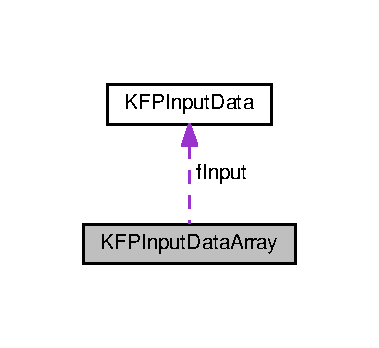
\includegraphics[width=182pt]{structKFPInputDataArray__coll__graph}
\end{center}
\end{figure}
\subsection*{Public Attributes}
\begin{DoxyCompactItemize}
\item 
\hyperlink{classKFPInputData}{K\+F\+P\+Input\+Data} $\ast$ \hyperlink{structKFPInputDataArray_ae22c5ff3cb181d5b676838cef57ae4c1}{f\+Input}\hypertarget{structKFPInputDataArray_ae22c5ff3cb181d5b676838cef57ae4c1}{}\label{structKFPInputDataArray_ae22c5ff3cb181d5b676838cef57ae4c1}

\begin{DoxyCompactList}\small\item\em Pointer to the array of the input data objects. \end{DoxyCompactList}\end{DoxyCompactItemize}


\subsection{Detailed Description}
Structure with the set of the input data for KF Particle Finder. 

\begin{DoxyAuthor}{Author}
M.\+Zyzak, I.\+Kisel 
\end{DoxyAuthor}
\begin{DoxyDate}{Date}
05.\+02.\+2019 
\end{DoxyDate}
\begin{DoxyVersion}{Version}
1.\+0
\end{DoxyVersion}
The structure contains pointer to array of \hyperlink{classKFPInputData}{K\+F\+P\+Input\+Data} objects. Copying of the objects of this structure is disabled. 

The documentation for this class was generated from the following file\+:\begin{DoxyCompactItemize}
\item 
/home/user/cbmdir/kfpf/\+K\+F\+Particle/\+K\+F\+Particle/K\+F\+P\+Input\+Data.\+h\end{DoxyCompactItemize}

\hypertarget{structKFPLinkedList}{}\section{K\+F\+P\+Linked\+List Class Reference}
\label{structKFPLinkedList}\index{K\+F\+P\+Linked\+List@{K\+F\+P\+Linked\+List}}


Structure to creat a linked list of the input data.  




{\ttfamily \#include $<$K\+F\+P\+Input\+Data.\+h$>$}



Collaboration diagram for K\+F\+P\+Linked\+List\+:
\nopagebreak
\begin{figure}[H]
\begin{center}
\leavevmode
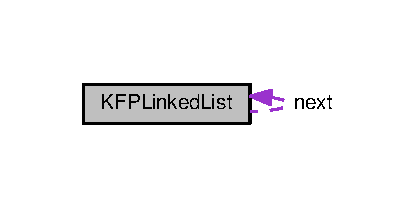
\includegraphics[width=200pt]{structKFPLinkedList__coll__graph}
\end{center}
\end{figure}
\subsection*{Public Member Functions}
\begin{DoxyCompactItemize}
\item 
void $\ast$ \hyperlink{structKFPLinkedList_af31a2b29ff463ab8b2895b9e10b18148}{operator new} (size\+\_\+t size)\hypertarget{structKFPLinkedList_af31a2b29ff463ab8b2895b9e10b18148}{}\label{structKFPLinkedList_af31a2b29ff463ab8b2895b9e10b18148}

\begin{DoxyCompactList}\small\item\em new operator for allocation of the S\+I\+M\+D-\/alligned dynamic memory allocation \end{DoxyCompactList}\item 
void $\ast$ \hyperlink{structKFPLinkedList_ad33eb6523ee7590def7627ff90e72165}{operator new\mbox{[}$\,$\mbox{]}} (size\+\_\+t size)\hypertarget{structKFPLinkedList_ad33eb6523ee7590def7627ff90e72165}{}\label{structKFPLinkedList_ad33eb6523ee7590def7627ff90e72165}

\begin{DoxyCompactList}\small\item\em new operator for allocation of the S\+I\+M\+D-\/alligned dynamic memory allocation \end{DoxyCompactList}\item 
void $\ast$ \hyperlink{structKFPLinkedList_afdd5878bcf17d951f5ab54d82fe3bf78}{operator new} (size\+\_\+t size, void $\ast$ptr)\hypertarget{structKFPLinkedList_afdd5878bcf17d951f5ab54d82fe3bf78}{}\label{structKFPLinkedList_afdd5878bcf17d951f5ab54d82fe3bf78}

\begin{DoxyCompactList}\small\item\em new operator for allocation of the S\+I\+M\+D-\/alligned dynamic memory allocation \end{DoxyCompactList}\item 
void $\ast$ \hyperlink{structKFPLinkedList_a1cf3274c5b9e4ce7380378b12ef491cb}{operator new\mbox{[}$\,$\mbox{]}} (size\+\_\+t size, void $\ast$ptr)\hypertarget{structKFPLinkedList_a1cf3274c5b9e4ce7380378b12ef491cb}{}\label{structKFPLinkedList_a1cf3274c5b9e4ce7380378b12ef491cb}

\begin{DoxyCompactList}\small\item\em new operator for allocation of the S\+I\+M\+D-\/alligned dynamic memory allocation \end{DoxyCompactList}\item 
void \hyperlink{structKFPLinkedList_aca525b27aa26f5884d9fa0088c195ea6}{operator delete} (void $\ast$ptr, size\+\_\+t)\hypertarget{structKFPLinkedList_aca525b27aa26f5884d9fa0088c195ea6}{}\label{structKFPLinkedList_aca525b27aa26f5884d9fa0088c195ea6}

\begin{DoxyCompactList}\small\item\em delete operator for the S\+I\+M\+D-\/alligned dynamic memory release \end{DoxyCompactList}\item 
void \hyperlink{structKFPLinkedList_ac22d49d82fbc8d45d2a01da5e55de6f1}{operator delete\mbox{[}$\,$\mbox{]}} (void $\ast$ptr, size\+\_\+t)\hypertarget{structKFPLinkedList_ac22d49d82fbc8d45d2a01da5e55de6f1}{}\label{structKFPLinkedList_ac22d49d82fbc8d45d2a01da5e55de6f1}

\begin{DoxyCompactList}\small\item\em delete operator for the S\+I\+M\+D-\/alligned dynamic memory release \end{DoxyCompactList}\item 
\hyperlink{classKFPInputData}{K\+F\+P\+Input\+Data} data \hyperlink{structKFPLinkedList_a0dcd70e475be19f41a205412301bdaf1}{\+\_\+\+\_\+attribute\+\_\+\+\_\+} ((aligned(sizeof(float\+\_\+v))))
\begin{DoxyCompactList}\small\item\em Input data for KF Particle Finder. \end{DoxyCompactList}\end{DoxyCompactItemize}
\subsection*{Public Attributes}
\begin{DoxyCompactItemize}
\item 
\hyperlink{structKFPLinkedList}{K\+F\+P\+Linked\+List} $\ast$ \hyperlink{structKFPLinkedList_aa528c23983df4be726b9b0cfd6e76d82}{next}\hypertarget{structKFPLinkedList_aa528c23983df4be726b9b0cfd6e76d82}{}\label{structKFPLinkedList_aa528c23983df4be726b9b0cfd6e76d82}

\begin{DoxyCompactList}\small\item\em Link to the nex object in the linked list. \end{DoxyCompactList}\end{DoxyCompactItemize}


\subsection{Detailed Description}
Structure to creat a linked list of the input data. 

\begin{DoxyAuthor}{Author}
M.\+Zyzak, I.\+Kisel 
\end{DoxyAuthor}
\begin{DoxyDate}{Date}
05.\+02.\+2019 
\end{DoxyDate}
\begin{DoxyVersion}{Version}
1.\+0
\end{DoxyVersion}
The structure contains pointer to array of \hyperlink{classKFPInputData}{K\+F\+P\+Input\+Data} objects. Copying of the objects of this structure is disabled. The list is used to create a queue for processing at the device side (Intel Xeon Phi). 

\subsection{Member Function Documentation}
\index{K\+F\+P\+Linked\+List@{K\+F\+P\+Linked\+List}!\+\_\+\+\_\+attribute\+\_\+\+\_\+@{\+\_\+\+\_\+attribute\+\_\+\+\_\+}}
\index{\+\_\+\+\_\+attribute\+\_\+\+\_\+@{\+\_\+\+\_\+attribute\+\_\+\+\_\+}!K\+F\+P\+Linked\+List@{K\+F\+P\+Linked\+List}}
\subsubsection[{\texorpdfstring{\+\_\+\+\_\+attribute\+\_\+\+\_\+((aligned(sizeof(float\+\_\+v))))}{__attribute__((aligned(sizeof(float_v))))}}]{\setlength{\rightskip}{0pt plus 5cm}{\bf K\+F\+P\+Input\+Data} data K\+F\+P\+Linked\+List\+::\+\_\+\+\_\+attribute\+\_\+\+\_\+ (
\begin{DoxyParamCaption}
\item[{(aligned(sizeof(float\+\_\+v)))}]{}
\end{DoxyParamCaption}
)}\hypertarget{structKFPLinkedList_a0dcd70e475be19f41a205412301bdaf1}{}\label{structKFPLinkedList_a0dcd70e475be19f41a205412301bdaf1}


Input data for KF Particle Finder. 

\begin{DoxySeeAlso}{See also}
\hyperlink{classKFPInputData}{K\+F\+P\+Input\+Data}. 
\end{DoxySeeAlso}


The documentation for this class was generated from the following file\+:\begin{DoxyCompactItemize}
\item 
/home/user/cbmdir/kfpf/\+K\+F\+Particle/\+K\+F\+Particle/K\+F\+P\+Input\+Data.\+h\end{DoxyCompactItemize}

\hypertarget{classKFPSimdAllocator}{}\section{K\+F\+P\+Simd\+Allocator$<$ T $>$ Class Template Reference}
\label{classKFPSimdAllocator}\index{K\+F\+P\+Simd\+Allocator$<$ T $>$@{K\+F\+P\+Simd\+Allocator$<$ T $>$}}


Allocator which is needed to allocate memory in std\+::vector aligned by the size of S\+I\+MD vectors.  




{\ttfamily \#include $<$K\+F\+P\+Simd\+Allocator.\+h$>$}

\subsection*{Classes}
\begin{DoxyCompactItemize}
\item 
class \hyperlink{structKFPSimdAllocator_1_1rebind}{rebind}
\begin{DoxyCompactList}\small\item\em Rebind allocator to type U of the S\+I\+MD allocator. \end{DoxyCompactList}\end{DoxyCompactItemize}
\subsection*{Public Types}
\begin{DoxyCompactItemize}
\item 
typedef T {\bfseries value\+\_\+type}\hypertarget{classKFPSimdAllocator_a2220f8e8df85a28528c3b638d6d3326e}{}\label{classKFPSimdAllocator_a2220f8e8df85a28528c3b638d6d3326e}

\item 
typedef T $\ast$ {\bfseries pointer}\hypertarget{classKFPSimdAllocator_a3be67dc1570711f43bffb59df7a101fb}{}\label{classKFPSimdAllocator_a3be67dc1570711f43bffb59df7a101fb}

\item 
typedef const T $\ast$ {\bfseries const\+\_\+pointer}\hypertarget{classKFPSimdAllocator_a9838e96bfdcbad5ea6a8f6634b0efec0}{}\label{classKFPSimdAllocator_a9838e96bfdcbad5ea6a8f6634b0efec0}

\item 
typedef T \& {\bfseries reference}\hypertarget{classKFPSimdAllocator_af718c8189940e57744a409091aa768b1}{}\label{classKFPSimdAllocator_af718c8189940e57744a409091aa768b1}

\item 
typedef const T \& {\bfseries const\+\_\+reference}\hypertarget{classKFPSimdAllocator_a545bff14e608d6a5d405f75cd9d7b3ec}{}\label{classKFPSimdAllocator_a545bff14e608d6a5d405f75cd9d7b3ec}

\item 
typedef std\+::size\+\_\+t {\bfseries size\+\_\+type}\hypertarget{classKFPSimdAllocator_a693ced984b2b34276785ff5bc27b5814}{}\label{classKFPSimdAllocator_a693ced984b2b34276785ff5bc27b5814}

\item 
typedef std\+::ptrdiff\+\_\+t {\bfseries difference\+\_\+type}\hypertarget{classKFPSimdAllocator_ab2c1ad95cf013d9239f090a5e695c38b}{}\label{classKFPSimdAllocator_ab2c1ad95cf013d9239f090a5e695c38b}

\end{DoxyCompactItemize}
\subsection*{Public Member Functions}
\begin{DoxyCompactItemize}
\item 
pointer \hyperlink{classKFPSimdAllocator_a940fe6fc661958ebd72c192b3cfd9732}{address} (reference value) const 
\item 
const\+\_\+pointer \hyperlink{classKFPSimdAllocator_a2b6cce7e6d21f8f61e6d9eb577f03176}{address} (const\+\_\+reference value) const 
\item 
{\bfseries K\+F\+P\+Simd\+Allocator} (const \hyperlink{classKFPSimdAllocator}{K\+F\+P\+Simd\+Allocator} \&)  throw ()\hypertarget{classKFPSimdAllocator_ae3c869f7146830e3aa51609aaa469a1b}{}\label{classKFPSimdAllocator_ae3c869f7146830e3aa51609aaa469a1b}

\item 
{\footnotesize template$<$class U $>$ }\\{\bfseries K\+F\+P\+Simd\+Allocator} (const \hyperlink{classKFPSimdAllocator}{K\+F\+P\+Simd\+Allocator}$<$ U $>$ \&)  throw ()\hypertarget{classKFPSimdAllocator_a519e1267b4c04f9d3c2edcbab9026f81}{}\label{classKFPSimdAllocator_a519e1267b4c04f9d3c2edcbab9026f81}

\item 
size\+\_\+type \hyperlink{classKFPSimdAllocator_a5cb432db266d47facaa932576c899602}{max\+\_\+size} () const   throw ()
\item 
pointer \hyperlink{classKFPSimdAllocator_a6112376bd53f74b5c360c5d9ee7d1867}{allocate} (size\+\_\+type num, const void $\ast$=nullptr)
\item 
void \hyperlink{classKFPSimdAllocator_a4e7732dacbbea0ed92224c9295d14f56}{construct} (pointer p)
\item 
void \hyperlink{classKFPSimdAllocator_a206aeadc9db52a9918be232606710eea}{construct} (pointer p, const T \&value)
\item 
void \hyperlink{classKFPSimdAllocator_a654bc8b82b27fe73c14e87d9f3a73b9e}{destroy} (pointer p)
\item 
void \hyperlink{classKFPSimdAllocator_a09742f45872a8568926482ba76f49762}{deallocate} (pointer p, size\+\_\+type num)
\item 
void $\ast$ \hyperlink{classKFPSimdAllocator_a04f7288a8003d7c446d194174faa9d85}{operator new} (size\+\_\+t size, void $\ast$ptr)\hypertarget{classKFPSimdAllocator_a04f7288a8003d7c446d194174faa9d85}{}\label{classKFPSimdAllocator_a04f7288a8003d7c446d194174faa9d85}

\begin{DoxyCompactList}\small\item\em new operator for allocation of the S\+I\+M\+D-\/alligned dynamic memory allocation \end{DoxyCompactList}\item 
void $\ast$ \hyperlink{classKFPSimdAllocator_a45c0c288c2790a41ab7e1eb30a974747}{operator new\mbox{[}$\,$\mbox{]}} (size\+\_\+t size, void $\ast$ptr)\hypertarget{classKFPSimdAllocator_a45c0c288c2790a41ab7e1eb30a974747}{}\label{classKFPSimdAllocator_a45c0c288c2790a41ab7e1eb30a974747}

\begin{DoxyCompactList}\small\item\em new operator for allocation of the S\+I\+M\+D-\/alligned dynamic memory allocation \end{DoxyCompactList}\item 
void $\ast$ \hyperlink{classKFPSimdAllocator_aecd37d22a3328bc3ab45af85280d683f}{operator new} (size\+\_\+t size)\hypertarget{classKFPSimdAllocator_aecd37d22a3328bc3ab45af85280d683f}{}\label{classKFPSimdAllocator_aecd37d22a3328bc3ab45af85280d683f}

\begin{DoxyCompactList}\small\item\em new operator for allocation of the S\+I\+M\+D-\/alligned dynamic memory allocation \end{DoxyCompactList}\item 
void $\ast$ \hyperlink{classKFPSimdAllocator_a52963f32ee363d10045d0c99cb4bf404}{operator new\mbox{[}$\,$\mbox{]}} (size\+\_\+t size)\hypertarget{classKFPSimdAllocator_a52963f32ee363d10045d0c99cb4bf404}{}\label{classKFPSimdAllocator_a52963f32ee363d10045d0c99cb4bf404}

\begin{DoxyCompactList}\small\item\em new operator for allocation of the S\+I\+M\+D-\/alligned dynamic memory allocation \end{DoxyCompactList}\item 
void \hyperlink{classKFPSimdAllocator_ab8878f29f6745fbf3dae25598fb7fe01}{operator delete} (void $\ast$ptr, size\+\_\+t)\hypertarget{classKFPSimdAllocator_ab8878f29f6745fbf3dae25598fb7fe01}{}\label{classKFPSimdAllocator_ab8878f29f6745fbf3dae25598fb7fe01}

\begin{DoxyCompactList}\small\item\em delete operator for the S\+I\+M\+D-\/alligned dynamic memory release \end{DoxyCompactList}\item 
void \hyperlink{classKFPSimdAllocator_acb81e29329e6a990cbcd4c82a8c72491}{operator delete\mbox{[}$\,$\mbox{]}} (void $\ast$ptr, size\+\_\+t)\hypertarget{classKFPSimdAllocator_acb81e29329e6a990cbcd4c82a8c72491}{}\label{classKFPSimdAllocator_acb81e29329e6a990cbcd4c82a8c72491}

\begin{DoxyCompactList}\small\item\em delete operator for the S\+I\+M\+D-\/alligned dynamic memory release \end{DoxyCompactList}\end{DoxyCompactItemize}


\subsection{Detailed Description}
\subsubsection*{template$<$class T$>$\\*
class K\+F\+P\+Simd\+Allocator$<$ T $>$}

Allocator which is needed to allocate memory in std\+::vector aligned by the size of S\+I\+MD vectors. 

\begin{DoxyAuthor}{Author}
M.\+Zyzak, I.\+Kisel 
\end{DoxyAuthor}
\begin{DoxyDate}{Date}
05.\+02.\+2019 
\end{DoxyDate}
\begin{DoxyVersion}{Version}
1.\+0 
\end{DoxyVersion}


\subsection{Member Function Documentation}
\index{K\+F\+P\+Simd\+Allocator@{K\+F\+P\+Simd\+Allocator}!address@{address}}
\index{address@{address}!K\+F\+P\+Simd\+Allocator@{K\+F\+P\+Simd\+Allocator}}
\subsubsection[{\texorpdfstring{address(reference value) const }{address(reference value) const }}]{\setlength{\rightskip}{0pt plus 5cm}template$<$class T $>$ pointer {\bf K\+F\+P\+Simd\+Allocator}$<$ T $>$\+::address (
\begin{DoxyParamCaption}
\item[{reference}]{value}
\end{DoxyParamCaption}
) const\hspace{0.3cm}{\ttfamily [inline]}}\hypertarget{classKFPSimdAllocator_a940fe6fc661958ebd72c192b3cfd9732}{}\label{classKFPSimdAllocator_a940fe6fc661958ebd72c192b3cfd9732}
Return address of \char`\"{}value\char`\"{}. \index{K\+F\+P\+Simd\+Allocator@{K\+F\+P\+Simd\+Allocator}!address@{address}}
\index{address@{address}!K\+F\+P\+Simd\+Allocator@{K\+F\+P\+Simd\+Allocator}}
\subsubsection[{\texorpdfstring{address(const\+\_\+reference value) const }{address(const_reference value) const }}]{\setlength{\rightskip}{0pt plus 5cm}template$<$class T $>$ const\+\_\+pointer {\bf K\+F\+P\+Simd\+Allocator}$<$ T $>$\+::address (
\begin{DoxyParamCaption}
\item[{const\+\_\+reference}]{value}
\end{DoxyParamCaption}
) const\hspace{0.3cm}{\ttfamily [inline]}}\hypertarget{classKFPSimdAllocator_a2b6cce7e6d21f8f61e6d9eb577f03176}{}\label{classKFPSimdAllocator_a2b6cce7e6d21f8f61e6d9eb577f03176}
Return address of \char`\"{}value\char`\"{}. \index{K\+F\+P\+Simd\+Allocator@{K\+F\+P\+Simd\+Allocator}!allocate@{allocate}}
\index{allocate@{allocate}!K\+F\+P\+Simd\+Allocator@{K\+F\+P\+Simd\+Allocator}}
\subsubsection[{\texorpdfstring{allocate(size\+\_\+type num, const void $\ast$=nullptr)}{allocate(size_type num, const void *=nullptr)}}]{\setlength{\rightskip}{0pt plus 5cm}template$<$class T $>$ pointer {\bf K\+F\+P\+Simd\+Allocator}$<$ T $>$\+::allocate (
\begin{DoxyParamCaption}
\item[{size\+\_\+type}]{num, }
\item[{const void $\ast$}]{ = {\ttfamily nullptr}}
\end{DoxyParamCaption}
)\hspace{0.3cm}{\ttfamily [inline]}}\hypertarget{classKFPSimdAllocator_a6112376bd53f74b5c360c5d9ee7d1867}{}\label{classKFPSimdAllocator_a6112376bd53f74b5c360c5d9ee7d1867}
Allocate but don\textquotesingle{}t initialize num elements of type T. \index{K\+F\+P\+Simd\+Allocator@{K\+F\+P\+Simd\+Allocator}!construct@{construct}}
\index{construct@{construct}!K\+F\+P\+Simd\+Allocator@{K\+F\+P\+Simd\+Allocator}}
\subsubsection[{\texorpdfstring{construct(pointer p)}{construct(pointer p)}}]{\setlength{\rightskip}{0pt plus 5cm}template$<$class T $>$ void {\bf K\+F\+P\+Simd\+Allocator}$<$ T $>$\+::construct (
\begin{DoxyParamCaption}
\item[{pointer}]{p}
\end{DoxyParamCaption}
)\hspace{0.3cm}{\ttfamily [inline]}}\hypertarget{classKFPSimdAllocator_a4e7732dacbbea0ed92224c9295d14f56}{}\label{classKFPSimdAllocator_a4e7732dacbbea0ed92224c9295d14f56}
Initialize elements of allocated storage \char`\"{}p\char`\"{} with an empty element. \index{K\+F\+P\+Simd\+Allocator@{K\+F\+P\+Simd\+Allocator}!construct@{construct}}
\index{construct@{construct}!K\+F\+P\+Simd\+Allocator@{K\+F\+P\+Simd\+Allocator}}
\subsubsection[{\texorpdfstring{construct(pointer p, const T \&value)}{construct(pointer p, const T &value)}}]{\setlength{\rightskip}{0pt plus 5cm}template$<$class T $>$ void {\bf K\+F\+P\+Simd\+Allocator}$<$ T $>$\+::construct (
\begin{DoxyParamCaption}
\item[{pointer}]{p, }
\item[{const T \&}]{value}
\end{DoxyParamCaption}
)\hspace{0.3cm}{\ttfamily [inline]}}\hypertarget{classKFPSimdAllocator_a206aeadc9db52a9918be232606710eea}{}\label{classKFPSimdAllocator_a206aeadc9db52a9918be232606710eea}
Initialize elements of allocated storage \char`\"{}p\char`\"{} with value \char`\"{}value\char`\"{}. \index{K\+F\+P\+Simd\+Allocator@{K\+F\+P\+Simd\+Allocator}!deallocate@{deallocate}}
\index{deallocate@{deallocate}!K\+F\+P\+Simd\+Allocator@{K\+F\+P\+Simd\+Allocator}}
\subsubsection[{\texorpdfstring{deallocate(pointer p, size\+\_\+type num)}{deallocate(pointer p, size_type num)}}]{\setlength{\rightskip}{0pt plus 5cm}template$<$class T $>$ void {\bf K\+F\+P\+Simd\+Allocator}$<$ T $>$\+::deallocate (
\begin{DoxyParamCaption}
\item[{pointer}]{p, }
\item[{size\+\_\+type}]{num}
\end{DoxyParamCaption}
)\hspace{0.3cm}{\ttfamily [inline]}}\hypertarget{classKFPSimdAllocator_a09742f45872a8568926482ba76f49762}{}\label{classKFPSimdAllocator_a09742f45872a8568926482ba76f49762}
Deallocate storage p of deleted elements. \index{K\+F\+P\+Simd\+Allocator@{K\+F\+P\+Simd\+Allocator}!destroy@{destroy}}
\index{destroy@{destroy}!K\+F\+P\+Simd\+Allocator@{K\+F\+P\+Simd\+Allocator}}
\subsubsection[{\texorpdfstring{destroy(pointer p)}{destroy(pointer p)}}]{\setlength{\rightskip}{0pt plus 5cm}template$<$class T $>$ void {\bf K\+F\+P\+Simd\+Allocator}$<$ T $>$\+::destroy (
\begin{DoxyParamCaption}
\item[{pointer}]{p}
\end{DoxyParamCaption}
)\hspace{0.3cm}{\ttfamily [inline]}}\hypertarget{classKFPSimdAllocator_a654bc8b82b27fe73c14e87d9f3a73b9e}{}\label{classKFPSimdAllocator_a654bc8b82b27fe73c14e87d9f3a73b9e}
Destroy elements of initialized storage \char`\"{}p\char`\"{}. \index{K\+F\+P\+Simd\+Allocator@{K\+F\+P\+Simd\+Allocator}!max\+\_\+size@{max\+\_\+size}}
\index{max\+\_\+size@{max\+\_\+size}!K\+F\+P\+Simd\+Allocator@{K\+F\+P\+Simd\+Allocator}}
\subsubsection[{\texorpdfstring{max\+\_\+size() const }{max_size() const }}]{\setlength{\rightskip}{0pt plus 5cm}template$<$class T $>$ size\+\_\+type {\bf K\+F\+P\+Simd\+Allocator}$<$ T $>$\+::max\+\_\+size (
\begin{DoxyParamCaption}
{}
\end{DoxyParamCaption}
) const throw  ) \hspace{0.3cm}{\ttfamily [inline]}}\hypertarget{classKFPSimdAllocator_a5cb432db266d47facaa932576c899602}{}\label{classKFPSimdAllocator_a5cb432db266d47facaa932576c899602}
Return maximum number of elements that can be allocated. 

The documentation for this class was generated from the following file\+:\begin{DoxyCompactItemize}
\item 
/home/user/cbmdir/kfpf/\+K\+F\+Particle/\+K\+F\+Particle/K\+F\+P\+Simd\+Allocator.\+h\end{DoxyCompactItemize}

\hypertarget{classKFPTrack}{}\section{K\+F\+P\+Track Class Reference}
\label{classKFPTrack}\index{K\+F\+P\+Track@{K\+F\+P\+Track}}


A scalar class for storage of the track in the cartesian parametrisation.  




{\ttfamily \#include $<$K\+F\+P\+Track.\+h$>$}

\subsection*{Public Member Functions}
\begin{DoxyCompactItemize}
\item 
int \hyperlink{classKFPTrack_a8d74655c104b6ee95d8cde2e0a10f091}{Get\+ID} () const \hypertarget{classKFPTrack_a8d74655c104b6ee95d8cde2e0a10f091}{}\label{classKFPTrack_a8d74655c104b6ee95d8cde2e0a10f091}

\begin{DoxyCompactList}\small\item\em Returns Id of the track. \end{DoxyCompactList}\item 
bool \hyperlink{classKFPTrack_a096ae252f6c0a83704896a4587076dc8}{Get\+X\+Y\+Z\+Px\+Py\+Pz} (float $\ast$p) const 
\item 
bool \hyperlink{classKFPTrack_adcb29beece55806f5fdbc740d31de90f}{Get\+Covariance\+X\+Y\+Z\+Px\+Py\+Pz} (float cv\mbox{[}21\mbox{]}) const 
\item 
bool \hyperlink{classKFPTrack_aba503f301fc0ad25eaf2b815514633c6}{Get\+Covariance\+X\+Y\+Z\+Px\+Py\+Pz} (double cv\mbox{[}21\mbox{]}) const 
\item 
void \hyperlink{classKFPTrack_a48c96dc9976b48fccf6eaadf8f31241a}{Get\+X\+YZ} (float $\ast$position) const 
\item 
void \hyperlink{classKFPTrack_ab4c776a3db93987d2c5298034fe3ea23}{Get\+Px\+Py\+Pz} (float $\ast$position) const 
\item 
void \hyperlink{classKFPTrack_a898efd7d653aa2a2c82f92c80cc3875f}{Xv\+Yv\+Zv} (float $\ast$position) const 
\item 
void \hyperlink{classKFPTrack_a4073f2dd7d0cb17a47906c352026855f}{Px\+Py\+Pz} (float $\ast$position) const 
\item 
void \hyperlink{classKFPTrack_adffcfd62628fcd28ed7068edb5505fec}{Xv\+Yv\+Zv} (double $\ast$position) const 
\item 
void \hyperlink{classKFPTrack_a92544f10b694cbde96d12d52f466492a}{Px\+Py\+Pz} (double $\ast$position) const 
\item 
float \hyperlink{classKFPTrack_a1975006b69521908be3c3684e9842fb9}{GetX} () const \hypertarget{classKFPTrack_a1975006b69521908be3c3684e9842fb9}{}\label{classKFPTrack_a1975006b69521908be3c3684e9842fb9}

\begin{DoxyCompactList}\small\item\em Returns X coordinate of the track. \end{DoxyCompactList}\item 
float \hyperlink{classKFPTrack_a49af0096efd8522003dff109ae3a15f0}{GetY} () const \hypertarget{classKFPTrack_a49af0096efd8522003dff109ae3a15f0}{}\label{classKFPTrack_a49af0096efd8522003dff109ae3a15f0}

\begin{DoxyCompactList}\small\item\em Returns Y coordinate of the track. \end{DoxyCompactList}\item 
float \hyperlink{classKFPTrack_a0291b116ad42cc695517a26d88b02621}{GetZ} () const \hypertarget{classKFPTrack_a0291b116ad42cc695517a26d88b02621}{}\label{classKFPTrack_a0291b116ad42cc695517a26d88b02621}

\begin{DoxyCompactList}\small\item\em Returns Z coordinate of the track. \end{DoxyCompactList}\item 
float \hyperlink{classKFPTrack_a2e24a47ade49d2e8a227374f4a443737}{Get\+Px} () const \hypertarget{classKFPTrack_a2e24a47ade49d2e8a227374f4a443737}{}\label{classKFPTrack_a2e24a47ade49d2e8a227374f4a443737}

\begin{DoxyCompactList}\small\item\em Returns Px component of the momentum of the track. \end{DoxyCompactList}\item 
float \hyperlink{classKFPTrack_a3b49837a7c04122f3b3b889dfa611a6a}{Get\+Py} () const \hypertarget{classKFPTrack_a3b49837a7c04122f3b3b889dfa611a6a}{}\label{classKFPTrack_a3b49837a7c04122f3b3b889dfa611a6a}

\begin{DoxyCompactList}\small\item\em Returns Py component of the momentum of the track. \end{DoxyCompactList}\item 
float \hyperlink{classKFPTrack_a5f711955ea21d5c26128f4992db253ad}{Get\+Pz} () const \hypertarget{classKFPTrack_a5f711955ea21d5c26128f4992db253ad}{}\label{classKFPTrack_a5f711955ea21d5c26128f4992db253ad}

\begin{DoxyCompactList}\small\item\em Returns Pz component of the momentum of the track. \end{DoxyCompactList}\item 
float \hyperlink{classKFPTrack_a65a744af280c0dc2356e3abbdbfbb2c3}{Get\+Pt} () const \hypertarget{classKFPTrack_a65a744af280c0dc2356e3abbdbfbb2c3}{}\label{classKFPTrack_a65a744af280c0dc2356e3abbdbfbb2c3}

\begin{DoxyCompactList}\small\item\em Returns Pt -\/ transverse momentum of the track. \end{DoxyCompactList}\item 
float \hyperlink{classKFPTrack_a0118d414f37afc4773db82ce6c70c9b0}{GetP} () const \hypertarget{classKFPTrack_a0118d414f37afc4773db82ce6c70c9b0}{}\label{classKFPTrack_a0118d414f37afc4773db82ce6c70c9b0}

\begin{DoxyCompactList}\small\item\em Returns P -\/ momentum of the track. \end{DoxyCompactList}\item 
void \hyperlink{classKFPTrack_a4cb9baefe05535b9d47a5267e47774b2}{Get\+Covariance\+Matrix} (float $\ast$covmatrix)
\item 
float \hyperlink{classKFPTrack_a26a2c40f1816f0d071b7fee5bab617eb}{Get\+Parameter} (int i) const 
\begin{DoxyCompactList}\small\item\em Returns parameter \char`\"{}i\char`\"{} of the track. \end{DoxyCompactList}\item 
float \hyperlink{classKFPTrack_a7c63b7a88111433c719b96d5ca7c4951}{Get\+Covariance} (int i) const 
\begin{DoxyCompactList}\small\item\em Returns element of the covariance matrix \char`\"{}i\char`\"{} of the track. \end{DoxyCompactList}\item 
int \hyperlink{classKFPTrack_a4080eeb7c9d6327f8262dd3635b98a85}{Charge} () const \hypertarget{classKFPTrack_a4080eeb7c9d6327f8262dd3635b98a85}{}\label{classKFPTrack_a4080eeb7c9d6327f8262dd3635b98a85}

\begin{DoxyCompactList}\small\item\em Returns charge of the track. \end{DoxyCompactList}\item 
float \hyperlink{classKFPTrack_ac182c19b8070a08d1592f8f40907df7a}{Get\+Chi2per\+N\+DF} () const \hypertarget{classKFPTrack_ac182c19b8070a08d1592f8f40907df7a}{}\label{classKFPTrack_ac182c19b8070a08d1592f8f40907df7a}

\begin{DoxyCompactList}\small\item\em Returns Chi2/\+N\+DF of the track, N\+DF is a number of degrees of freedom. \end{DoxyCompactList}\item 
float \hyperlink{classKFPTrack_a6d3642d6ac5b7eddf9b673f94fea8d2c}{Get\+Chi2} () const \hypertarget{classKFPTrack_a6d3642d6ac5b7eddf9b673f94fea8d2c}{}\label{classKFPTrack_a6d3642d6ac5b7eddf9b673f94fea8d2c}

\begin{DoxyCompactList}\small\item\em Returns Chi2 of the track. \end{DoxyCompactList}\item 
int \hyperlink{classKFPTrack_a88971322ae4f8eec3be97aecab4fdea9}{Get\+N\+DF} () const \hypertarget{classKFPTrack_a88971322ae4f8eec3be97aecab4fdea9}{}\label{classKFPTrack_a88971322ae4f8eec3be97aecab4fdea9}

\begin{DoxyCompactList}\small\item\em Returns number of degrees of freedom of the track. \end{DoxyCompactList}\item 
const float $\ast$ \hyperlink{classKFPTrack_a9bd864f517bb22ac8374017fe57c1eae}{Get\+Track} () const \hypertarget{classKFPTrack_a9bd864f517bb22ac8374017fe57c1eae}{}\label{classKFPTrack_a9bd864f517bb22ac8374017fe57c1eae}

\begin{DoxyCompactList}\small\item\em Returns a pointer to the array of track parameters. \end{DoxyCompactList}\item 
const float $\ast$ \hyperlink{classKFPTrack_ac630ae470f31356547bb7d57cc0b151a}{Get\+Cov\+Matrix} () const \hypertarget{classKFPTrack_ac630ae470f31356547bb7d57cc0b151a}{}\label{classKFPTrack_ac630ae470f31356547bb7d57cc0b151a}

\begin{DoxyCompactList}\small\item\em Returns a pointer to the array of the covariance matrix elements stored in a lower triangular form. \end{DoxyCompactList}\item 
void \hyperlink{classKFPTrack_aa139b096b5a3ae8d89144021a9edae5e}{Set\+Parameters} (const float $\ast$position)
\item 
void \hyperlink{classKFPTrack_a609e11cfc6b3d20fb9ecb7f80b8b34c5}{Set\+Parameters} (double $\ast$position)
\item 
void \hyperlink{classKFPTrack_a34415422f378a08eda2d855870296fa2}{Set\+Parameters} (float x, float y, float z, float px, float py, float pz)
\item 
void \hyperlink{classKFPTrack_a2b526ac60d6cc17e216674dfbbdec969}{Set\+X\+YZ} (float x, float y, float z)
\item 
void \hyperlink{classKFPTrack_a69cac0d9ff19a76f15ddac24e7f30da4}{Set\+Px\+Py\+Pz} (float px, float py, float pz)
\item 
void \hyperlink{classKFPTrack_a0d4b6c1f619ab583e490b5fce4a22d3f}{Set\+ID} (int id)\hypertarget{classKFPTrack_a0d4b6c1f619ab583e490b5fce4a22d3f}{}\label{classKFPTrack_a0d4b6c1f619ab583e490b5fce4a22d3f}

\begin{DoxyCompactList}\small\item\em Sets Id of the track. \end{DoxyCompactList}\item 
void \hyperlink{classKFPTrack_a03bcf3402d7b5bd1c9f4cb716eaa62dc}{SetX} (float x)\hypertarget{classKFPTrack_a03bcf3402d7b5bd1c9f4cb716eaa62dc}{}\label{classKFPTrack_a03bcf3402d7b5bd1c9f4cb716eaa62dc}

\begin{DoxyCompactList}\small\item\em Sets X coordinate of the track. \end{DoxyCompactList}\item 
void \hyperlink{classKFPTrack_ae468ba33ada28608b1985a4115510aad}{SetY} (float y)\hypertarget{classKFPTrack_ae468ba33ada28608b1985a4115510aad}{}\label{classKFPTrack_ae468ba33ada28608b1985a4115510aad}

\begin{DoxyCompactList}\small\item\em Sets Y coordinate of the track. \end{DoxyCompactList}\item 
void \hyperlink{classKFPTrack_af74b945dba5f6889b9a2686e5284ba8e}{SetZ} (float z)\hypertarget{classKFPTrack_af74b945dba5f6889b9a2686e5284ba8e}{}\label{classKFPTrack_af74b945dba5f6889b9a2686e5284ba8e}

\begin{DoxyCompactList}\small\item\em Sets Z coordinate of the track. \end{DoxyCompactList}\item 
void \hyperlink{classKFPTrack_a5dbd5dd356267eaa55c12b43ba2533eb}{Set\+Px} (float px)\hypertarget{classKFPTrack_a5dbd5dd356267eaa55c12b43ba2533eb}{}\label{classKFPTrack_a5dbd5dd356267eaa55c12b43ba2533eb}

\begin{DoxyCompactList}\small\item\em Sets Px component of the track momentum. \end{DoxyCompactList}\item 
void \hyperlink{classKFPTrack_abf791820f24b3a23915b5b5cccd9f37d}{Set\+Py} (float py)\hypertarget{classKFPTrack_abf791820f24b3a23915b5b5cccd9f37d}{}\label{classKFPTrack_abf791820f24b3a23915b5b5cccd9f37d}

\begin{DoxyCompactList}\small\item\em Sets Py component of the track momentum. \end{DoxyCompactList}\item 
void \hyperlink{classKFPTrack_aa91b2f4354dcdfe167c82b416a26aa69}{Set\+Pz} (float pz)\hypertarget{classKFPTrack_aa91b2f4354dcdfe167c82b416a26aa69}{}\label{classKFPTrack_aa91b2f4354dcdfe167c82b416a26aa69}

\begin{DoxyCompactList}\small\item\em Sets Pz component of the track momentum. \end{DoxyCompactList}\item 
void \hyperlink{classKFPTrack_af0916c90726a14f3976c70452a5292a9}{Set\+Charge} (int q)\hypertarget{classKFPTrack_af0916c90726a14f3976c70452a5292a9}{}\label{classKFPTrack_af0916c90726a14f3976c70452a5292a9}

\begin{DoxyCompactList}\small\item\em Sets charge of the track. \end{DoxyCompactList}\item 
void \hyperlink{classKFPTrack_a1159ffc107e5df082590f0777f30fea8}{Set\+Chi2} (float chi)\hypertarget{classKFPTrack_a1159ffc107e5df082590f0777f30fea8}{}\label{classKFPTrack_a1159ffc107e5df082590f0777f30fea8}

\begin{DoxyCompactList}\small\item\em Sets a value of the track Chi2. \end{DoxyCompactList}\item 
void \hyperlink{classKFPTrack_aafb79cf24a433a293f05c2c3336d0d21}{Set\+N\+DF} (int ndf)\hypertarget{classKFPTrack_aafb79cf24a433a293f05c2c3336d0d21}{}\label{classKFPTrack_aafb79cf24a433a293f05c2c3336d0d21}

\begin{DoxyCompactList}\small\item\em Sets a value of the number of degrees of freedom. \end{DoxyCompactList}\item 
void \hyperlink{classKFPTrack_a105dc3b9dc17e979cc782492458ab88a}{Set\+Covariance\+Matrix} (const float $\ast$C)
\item 
void \hyperlink{classKFPTrack_a9b25532afa0f49ebfcedce044f74c349}{Set\+Covariance\+Matrix} (const double $\ast$C)
\item 
void \hyperlink{classKFPTrack_a1a524473353d515086af621107dea2fe}{Set\+Covariance} (const int i, const float c)
\item 
void \hyperlink{classKFPTrack_a3d9a9456222119b926cce3886bf15161}{Rotate\+XY} (float alpha)
\item 
int \hyperlink{classKFPTrack_a5ac4370d9be316566f3ef2e27edc9444}{Id} () const \hypertarget{classKFPTrack_a5ac4370d9be316566f3ef2e27edc9444}{}\label{classKFPTrack_a5ac4370d9be316566f3ef2e27edc9444}

\begin{DoxyCompactList}\small\item\em Returns Id of the track. \end{DoxyCompactList}\item 
void \hyperlink{classKFPTrack_a700911f0fb98e7914328f2f35b62166a}{Set\+Id} (int id)\hypertarget{classKFPTrack_a700911f0fb98e7914328f2f35b62166a}{}\label{classKFPTrack_a700911f0fb98e7914328f2f35b62166a}

\begin{DoxyCompactList}\small\item\em Sets Id of the track. \end{DoxyCompactList}\end{DoxyCompactItemize}


\subsection{Detailed Description}
A scalar class for storage of the track in the cartesian parametrisation. 

\begin{DoxyAuthor}{Author}
M.\+Zyzak, I.\+Kisel 
\end{DoxyAuthor}
\begin{DoxyDate}{Date}
05.\+02.\+2019 
\end{DoxyDate}
\begin{DoxyVersion}{Version}
1.\+0
\end{DoxyVersion}
A track is described with the state vector \{ X, Y, Z, Px, Py, Pz \} and the corresponding covariance matrix. Also contains charge of the track, chi2 of the track fit, the corresponding number of degrees of freedom, the unique Id of the track and the field approximation along the track trajectory. 

\subsection{Member Function Documentation}
\index{K\+F\+P\+Track@{K\+F\+P\+Track}!Get\+Covariance@{Get\+Covariance}}
\index{Get\+Covariance@{Get\+Covariance}!K\+F\+P\+Track@{K\+F\+P\+Track}}
\subsubsection[{\texorpdfstring{Get\+Covariance(int i) const }{GetCovariance(int i) const }}]{\setlength{\rightskip}{0pt plus 5cm}float K\+F\+P\+Track\+::\+Get\+Covariance (
\begin{DoxyParamCaption}
\item[{int}]{i}
\end{DoxyParamCaption}
) const\hspace{0.3cm}{\ttfamily [inline]}}\hypertarget{classKFPTrack_a7c63b7a88111433c719b96d5ca7c4951}{}\label{classKFPTrack_a7c63b7a88111433c719b96d5ca7c4951}


Returns element of the covariance matrix \char`\"{}i\char`\"{} of the track. 


\begin{DoxyParams}[1]{Parameters}
\mbox{\tt in}  & {\em i} & -\/ index of the element to be returned \\
\hline
\end{DoxyParams}
\index{K\+F\+P\+Track@{K\+F\+P\+Track}!Get\+Covariance\+Matrix@{Get\+Covariance\+Matrix}}
\index{Get\+Covariance\+Matrix@{Get\+Covariance\+Matrix}!K\+F\+P\+Track@{K\+F\+P\+Track}}
\subsubsection[{\texorpdfstring{Get\+Covariance\+Matrix(float $\ast$covmatrix)}{GetCovarianceMatrix(float *covmatrix)}}]{\setlength{\rightskip}{0pt plus 5cm}void K\+F\+P\+Track\+::\+Get\+Covariance\+Matrix (
\begin{DoxyParamCaption}
\item[{float $\ast$}]{covmatrix}
\end{DoxyParamCaption}
)\hspace{0.3cm}{\ttfamily [inline]}}\hypertarget{classKFPTrack_a4cb9baefe05535b9d47a5267e47774b2}{}\label{classKFPTrack_a4cb9baefe05535b9d47a5267e47774b2}
Copies the covariance matrix of the track to the array of floats. 
\begin{DoxyParams}[1]{Parameters}
\mbox{\tt out}  & {\em covmatrix\mbox{[}21\mbox{]}} & -\/ the output array, where the covariance matrix is copied\\
\hline
\end{DoxyParams}
\index{K\+F\+P\+Track@{K\+F\+P\+Track}!Get\+Covariance\+X\+Y\+Z\+Px\+Py\+Pz@{Get\+Covariance\+X\+Y\+Z\+Px\+Py\+Pz}}
\index{Get\+Covariance\+X\+Y\+Z\+Px\+Py\+Pz@{Get\+Covariance\+X\+Y\+Z\+Px\+Py\+Pz}!K\+F\+P\+Track@{K\+F\+P\+Track}}
\subsubsection[{\texorpdfstring{Get\+Covariance\+X\+Y\+Z\+Px\+Py\+Pz(float cv[21]) const }{GetCovarianceXYZPxPyPz(float cv[21]) const }}]{\setlength{\rightskip}{0pt plus 5cm}bool K\+F\+P\+Track\+::\+Get\+Covariance\+X\+Y\+Z\+Px\+Py\+Pz (
\begin{DoxyParamCaption}
\item[{float}]{cv\mbox{[}21\mbox{]}}
\end{DoxyParamCaption}
) const\hspace{0.3cm}{\ttfamily [inline]}}\hypertarget{classKFPTrack_adcb29beece55806f5fdbc740d31de90f}{}\label{classKFPTrack_adcb29beece55806f5fdbc740d31de90f}
Copies the covariance matrix of the track to the array of floats. 
\begin{DoxyParams}[1]{Parameters}
\mbox{\tt out}  & {\em cv\mbox{[}21\mbox{]}} & -\/ the output array, where the covariance matrix is copied\\
\hline
\end{DoxyParams}
\index{K\+F\+P\+Track@{K\+F\+P\+Track}!Get\+Covariance\+X\+Y\+Z\+Px\+Py\+Pz@{Get\+Covariance\+X\+Y\+Z\+Px\+Py\+Pz}}
\index{Get\+Covariance\+X\+Y\+Z\+Px\+Py\+Pz@{Get\+Covariance\+X\+Y\+Z\+Px\+Py\+Pz}!K\+F\+P\+Track@{K\+F\+P\+Track}}
\subsubsection[{\texorpdfstring{Get\+Covariance\+X\+Y\+Z\+Px\+Py\+Pz(double cv[21]) const }{GetCovarianceXYZPxPyPz(double cv[21]) const }}]{\setlength{\rightskip}{0pt plus 5cm}bool K\+F\+P\+Track\+::\+Get\+Covariance\+X\+Y\+Z\+Px\+Py\+Pz (
\begin{DoxyParamCaption}
\item[{double}]{cv\mbox{[}21\mbox{]}}
\end{DoxyParamCaption}
) const\hspace{0.3cm}{\ttfamily [inline]}}\hypertarget{classKFPTrack_aba503f301fc0ad25eaf2b815514633c6}{}\label{classKFPTrack_aba503f301fc0ad25eaf2b815514633c6}
Copies the covariance matrix of the track to the array of doubles. 
\begin{DoxyParams}[1]{Parameters}
\mbox{\tt out}  & {\em cv\mbox{[}21\mbox{]}} & -\/ the output array, where the covariance matrix is copied\\
\hline
\end{DoxyParams}
\index{K\+F\+P\+Track@{K\+F\+P\+Track}!Get\+Parameter@{Get\+Parameter}}
\index{Get\+Parameter@{Get\+Parameter}!K\+F\+P\+Track@{K\+F\+P\+Track}}
\subsubsection[{\texorpdfstring{Get\+Parameter(int i) const }{GetParameter(int i) const }}]{\setlength{\rightskip}{0pt plus 5cm}float K\+F\+P\+Track\+::\+Get\+Parameter (
\begin{DoxyParamCaption}
\item[{int}]{i}
\end{DoxyParamCaption}
) const\hspace{0.3cm}{\ttfamily [inline]}}\hypertarget{classKFPTrack_a26a2c40f1816f0d071b7fee5bab617eb}{}\label{classKFPTrack_a26a2c40f1816f0d071b7fee5bab617eb}


Returns parameter \char`\"{}i\char`\"{} of the track. 


\begin{DoxyParams}[1]{Parameters}
\mbox{\tt in}  & {\em i} & -\/ index of the parameter to be returned \\
\hline
\end{DoxyParams}
\index{K\+F\+P\+Track@{K\+F\+P\+Track}!Get\+Px\+Py\+Pz@{Get\+Px\+Py\+Pz}}
\index{Get\+Px\+Py\+Pz@{Get\+Px\+Py\+Pz}!K\+F\+P\+Track@{K\+F\+P\+Track}}
\subsubsection[{\texorpdfstring{Get\+Px\+Py\+Pz(float $\ast$position) const }{GetPxPyPz(float *position) const }}]{\setlength{\rightskip}{0pt plus 5cm}void K\+F\+P\+Track\+::\+Get\+Px\+Py\+Pz (
\begin{DoxyParamCaption}
\item[{float $\ast$}]{position}
\end{DoxyParamCaption}
) const\hspace{0.3cm}{\ttfamily [inline]}}\hypertarget{classKFPTrack_ab4c776a3db93987d2c5298034fe3ea23}{}\label{classKFPTrack_ab4c776a3db93987d2c5298034fe3ea23}
Copies 3 momentum components of the track to the output array of floats. 
\begin{DoxyParams}[1]{Parameters}
\mbox{\tt out}  & {\em position} & -\/ the output array with the momentum of the track \\
\hline
\end{DoxyParams}
\index{K\+F\+P\+Track@{K\+F\+P\+Track}!Get\+X\+YZ@{Get\+X\+YZ}}
\index{Get\+X\+YZ@{Get\+X\+YZ}!K\+F\+P\+Track@{K\+F\+P\+Track}}
\subsubsection[{\texorpdfstring{Get\+X\+Y\+Z(float $\ast$position) const }{GetXYZ(float *position) const }}]{\setlength{\rightskip}{0pt plus 5cm}void K\+F\+P\+Track\+::\+Get\+X\+YZ (
\begin{DoxyParamCaption}
\item[{float $\ast$}]{position}
\end{DoxyParamCaption}
) const\hspace{0.3cm}{\ttfamily [inline]}}\hypertarget{classKFPTrack_a48c96dc9976b48fccf6eaadf8f31241a}{}\label{classKFPTrack_a48c96dc9976b48fccf6eaadf8f31241a}
Copies position of the track to the output array of floats. 
\begin{DoxyParams}[1]{Parameters}
\mbox{\tt out}  & {\em position} & -\/ the output array with the position of the track \\
\hline
\end{DoxyParams}
\index{K\+F\+P\+Track@{K\+F\+P\+Track}!Get\+X\+Y\+Z\+Px\+Py\+Pz@{Get\+X\+Y\+Z\+Px\+Py\+Pz}}
\index{Get\+X\+Y\+Z\+Px\+Py\+Pz@{Get\+X\+Y\+Z\+Px\+Py\+Pz}!K\+F\+P\+Track@{K\+F\+P\+Track}}
\subsubsection[{\texorpdfstring{Get\+X\+Y\+Z\+Px\+Py\+Pz(float $\ast$p) const }{GetXYZPxPyPz(float *p) const }}]{\setlength{\rightskip}{0pt plus 5cm}bool K\+F\+P\+Track\+::\+Get\+X\+Y\+Z\+Px\+Py\+Pz (
\begin{DoxyParamCaption}
\item[{float $\ast$}]{p}
\end{DoxyParamCaption}
) const\hspace{0.3cm}{\ttfamily [inline]}}\hypertarget{classKFPTrack_a096ae252f6c0a83704896a4587076dc8}{}\label{classKFPTrack_a096ae252f6c0a83704896a4587076dc8}
Fills an array p with the parameters of the track. 
\begin{DoxyParams}[1]{Parameters}
\mbox{\tt out}  & {\em p} & -\/ array where \{ X, Y, Z, Px, Py, Pz \} are copied\\
\hline
\end{DoxyParams}
\index{K\+F\+P\+Track@{K\+F\+P\+Track}!Px\+Py\+Pz@{Px\+Py\+Pz}}
\index{Px\+Py\+Pz@{Px\+Py\+Pz}!K\+F\+P\+Track@{K\+F\+P\+Track}}
\subsubsection[{\texorpdfstring{Px\+Py\+Pz(float $\ast$position) const }{PxPyPz(float *position) const }}]{\setlength{\rightskip}{0pt plus 5cm}void K\+F\+P\+Track\+::\+Px\+Py\+Pz (
\begin{DoxyParamCaption}
\item[{float $\ast$}]{position}
\end{DoxyParamCaption}
) const\hspace{0.3cm}{\ttfamily [inline]}}\hypertarget{classKFPTrack_a4073f2dd7d0cb17a47906c352026855f}{}\label{classKFPTrack_a4073f2dd7d0cb17a47906c352026855f}
Copies 3 momentum components of the track to the output array of floats. 
\begin{DoxyParams}[1]{Parameters}
\mbox{\tt out}  & {\em position} & -\/ the output array with the momentum of the track \\
\hline
\end{DoxyParams}
\index{K\+F\+P\+Track@{K\+F\+P\+Track}!Px\+Py\+Pz@{Px\+Py\+Pz}}
\index{Px\+Py\+Pz@{Px\+Py\+Pz}!K\+F\+P\+Track@{K\+F\+P\+Track}}
\subsubsection[{\texorpdfstring{Px\+Py\+Pz(double $\ast$position) const }{PxPyPz(double *position) const }}]{\setlength{\rightskip}{0pt plus 5cm}void K\+F\+P\+Track\+::\+Px\+Py\+Pz (
\begin{DoxyParamCaption}
\item[{double $\ast$}]{position}
\end{DoxyParamCaption}
) const\hspace{0.3cm}{\ttfamily [inline]}}\hypertarget{classKFPTrack_a92544f10b694cbde96d12d52f466492a}{}\label{classKFPTrack_a92544f10b694cbde96d12d52f466492a}
Copies 3 momentum components of the track to the output array of doubles. 
\begin{DoxyParams}[1]{Parameters}
\mbox{\tt out}  & {\em position} & -\/ the output array with the momentum of the track \\
\hline
\end{DoxyParams}
\index{K\+F\+P\+Track@{K\+F\+P\+Track}!Rotate\+XY@{Rotate\+XY}}
\index{Rotate\+XY@{Rotate\+XY}!K\+F\+P\+Track@{K\+F\+P\+Track}}
\subsubsection[{\texorpdfstring{Rotate\+X\+Y(float alpha)}{RotateXY(float alpha)}}]{\setlength{\rightskip}{0pt plus 5cm}void K\+F\+P\+Track\+::\+Rotate\+XY (
\begin{DoxyParamCaption}
\item[{float}]{alpha}
\end{DoxyParamCaption}
)}\hypertarget{classKFPTrack_a3d9a9456222119b926cce3886bf15161}{}\label{classKFPTrack_a3d9a9456222119b926cce3886bf15161}
Rotates the parameters of the track on an angle alpha in the XY plane. Can be used in case of the transforamtion of the coordinate system. The rotation matrix is\+: \begin{DoxyVerb}{  cos(A), -sin(A),  0,        0,        0,   0 }
{  sin(A),  cos(A),  0,        0,        0,   0 }
{       0,       0,  1,        0,        0,   0 }
{       0,       0,  0,   cos(A),  -sin(A),   0 }
{       0,       0,  0,   sin(A),   cos(A),   0 }
{       0,       0,  0,        0,        0,   1 } 
\end{DoxyVerb}
 
\begin{DoxyParams}[1]{Parameters}
\mbox{\tt in}  & {\em alpha} & -\/ rotation angle\\
\hline
\end{DoxyParams}
\index{K\+F\+P\+Track@{K\+F\+P\+Track}!Set\+Covariance@{Set\+Covariance}}
\index{Set\+Covariance@{Set\+Covariance}!K\+F\+P\+Track@{K\+F\+P\+Track}}
\subsubsection[{\texorpdfstring{Set\+Covariance(const int i, const float c)}{SetCovariance(const int i, const float c)}}]{\setlength{\rightskip}{0pt plus 5cm}void K\+F\+P\+Track\+::\+Set\+Covariance (
\begin{DoxyParamCaption}
\item[{const int}]{i, }
\item[{const float}]{c}
\end{DoxyParamCaption}
)\hspace{0.3cm}{\ttfamily [inline]}}\hypertarget{classKFPTrack_a1a524473353d515086af621107dea2fe}{}\label{classKFPTrack_a1a524473353d515086af621107dea2fe}
Sets an element of the covariance matrix with index \char`\"{}i\char`\"{}. 
\begin{DoxyParams}[1]{Parameters}
\mbox{\tt in}  & {\em c} & -\/ value to be set \\
\hline
\mbox{\tt in}  & {\em i} & -\/ index of the element \\
\hline
\end{DoxyParams}
\index{K\+F\+P\+Track@{K\+F\+P\+Track}!Set\+Covariance\+Matrix@{Set\+Covariance\+Matrix}}
\index{Set\+Covariance\+Matrix@{Set\+Covariance\+Matrix}!K\+F\+P\+Track@{K\+F\+P\+Track}}
\subsubsection[{\texorpdfstring{Set\+Covariance\+Matrix(const float $\ast$\+C)}{SetCovarianceMatrix(const float *C)}}]{\setlength{\rightskip}{0pt plus 5cm}void K\+F\+P\+Track\+::\+Set\+Covariance\+Matrix (
\begin{DoxyParamCaption}
\item[{const float $\ast$}]{C}
\end{DoxyParamCaption}
)\hspace{0.3cm}{\ttfamily [inline]}}\hypertarget{classKFPTrack_a105dc3b9dc17e979cc782492458ab88a}{}\label{classKFPTrack_a105dc3b9dc17e979cc782492458ab88a}
Sets the covariance matrix from the input array of floats. 
\begin{DoxyParams}[1]{Parameters}
\mbox{\tt in}  & {\em C\mbox{[}21\mbox{]}} & -\/ array with the input elements of the covariance matrix stored in the lower triangular form\\
\hline
\end{DoxyParams}
\index{K\+F\+P\+Track@{K\+F\+P\+Track}!Set\+Covariance\+Matrix@{Set\+Covariance\+Matrix}}
\index{Set\+Covariance\+Matrix@{Set\+Covariance\+Matrix}!K\+F\+P\+Track@{K\+F\+P\+Track}}
\subsubsection[{\texorpdfstring{Set\+Covariance\+Matrix(const double $\ast$\+C)}{SetCovarianceMatrix(const double *C)}}]{\setlength{\rightskip}{0pt plus 5cm}void K\+F\+P\+Track\+::\+Set\+Covariance\+Matrix (
\begin{DoxyParamCaption}
\item[{const double $\ast$}]{C}
\end{DoxyParamCaption}
)\hspace{0.3cm}{\ttfamily [inline]}}\hypertarget{classKFPTrack_a9b25532afa0f49ebfcedce044f74c349}{}\label{classKFPTrack_a9b25532afa0f49ebfcedce044f74c349}
Sets the covariance matrix from the input array of doubles. 
\begin{DoxyParams}[1]{Parameters}
\mbox{\tt in}  & {\em C\mbox{[}21\mbox{]}} & -\/ array with the input elements of the covariance matrix stored in the lower triangular form\\
\hline
\end{DoxyParams}
\index{K\+F\+P\+Track@{K\+F\+P\+Track}!Set\+Parameters@{Set\+Parameters}}
\index{Set\+Parameters@{Set\+Parameters}!K\+F\+P\+Track@{K\+F\+P\+Track}}
\subsubsection[{\texorpdfstring{Set\+Parameters(const float $\ast$position)}{SetParameters(const float *position)}}]{\setlength{\rightskip}{0pt plus 5cm}void K\+F\+P\+Track\+::\+Set\+Parameters (
\begin{DoxyParamCaption}
\item[{const float $\ast$}]{position}
\end{DoxyParamCaption}
)\hspace{0.3cm}{\ttfamily [inline]}}\hypertarget{classKFPTrack_aa139b096b5a3ae8d89144021a9edae5e}{}\label{classKFPTrack_aa139b096b5a3ae8d89144021a9edae5e}
Sets parameters \{ X, Y, Z, Px, Py, Pz \} of the track from the input array of floats. 
\begin{DoxyParams}[1]{Parameters}
\mbox{\tt in}  & {\em position} & -\/ input array with the track parameters\\
\hline
\end{DoxyParams}
\index{K\+F\+P\+Track@{K\+F\+P\+Track}!Set\+Parameters@{Set\+Parameters}}
\index{Set\+Parameters@{Set\+Parameters}!K\+F\+P\+Track@{K\+F\+P\+Track}}
\subsubsection[{\texorpdfstring{Set\+Parameters(double $\ast$position)}{SetParameters(double *position)}}]{\setlength{\rightskip}{0pt plus 5cm}void K\+F\+P\+Track\+::\+Set\+Parameters (
\begin{DoxyParamCaption}
\item[{double $\ast$}]{position}
\end{DoxyParamCaption}
)\hspace{0.3cm}{\ttfamily [inline]}}\hypertarget{classKFPTrack_a609e11cfc6b3d20fb9ecb7f80b8b34c5}{}\label{classKFPTrack_a609e11cfc6b3d20fb9ecb7f80b8b34c5}
Sets parameters \{ X, Y, Z, Px, Py, Pz \} of the track from the input array of doubles. 
\begin{DoxyParams}[1]{Parameters}
\mbox{\tt in}  & {\em position} & -\/ input array with the track parameters\\
\hline
\end{DoxyParams}
\index{K\+F\+P\+Track@{K\+F\+P\+Track}!Set\+Parameters@{Set\+Parameters}}
\index{Set\+Parameters@{Set\+Parameters}!K\+F\+P\+Track@{K\+F\+P\+Track}}
\subsubsection[{\texorpdfstring{Set\+Parameters(float x, float y, float z, float px, float py, float pz)}{SetParameters(float x, float y, float z, float px, float py, float pz)}}]{\setlength{\rightskip}{0pt plus 5cm}void K\+F\+P\+Track\+::\+Set\+Parameters (
\begin{DoxyParamCaption}
\item[{float}]{x, }
\item[{float}]{y, }
\item[{float}]{z, }
\item[{float}]{px, }
\item[{float}]{py, }
\item[{float}]{pz}
\end{DoxyParamCaption}
)\hspace{0.3cm}{\ttfamily [inline]}}\hypertarget{classKFPTrack_a34415422f378a08eda2d855870296fa2}{}\label{classKFPTrack_a34415422f378a08eda2d855870296fa2}
Sets parameters \{ X, Y, Z, Px, Py, Pz \} of the track. 
\begin{DoxyParams}[1]{Parameters}
\mbox{\tt in}  & {\em x} & -\/ X coordinate to be set \\
\hline
\mbox{\tt in}  & {\em y} & -\/ Y coordinate to be set \\
\hline
\mbox{\tt in}  & {\em z} & -\/ Z coordinate to be set \\
\hline
\mbox{\tt in}  & {\em Px} & -\/ Px momentum component to be set \\
\hline
\mbox{\tt in}  & {\em Py} & -\/ Py momentum component to be set \\
\hline
\mbox{\tt in}  & {\em Pz} & -\/ Pz momentum component to be set\\
\hline
\end{DoxyParams}
\index{K\+F\+P\+Track@{K\+F\+P\+Track}!Set\+Px\+Py\+Pz@{Set\+Px\+Py\+Pz}}
\index{Set\+Px\+Py\+Pz@{Set\+Px\+Py\+Pz}!K\+F\+P\+Track@{K\+F\+P\+Track}}
\subsubsection[{\texorpdfstring{Set\+Px\+Py\+Pz(float px, float py, float pz)}{SetPxPyPz(float px, float py, float pz)}}]{\setlength{\rightskip}{0pt plus 5cm}void K\+F\+P\+Track\+::\+Set\+Px\+Py\+Pz (
\begin{DoxyParamCaption}
\item[{float}]{px, }
\item[{float}]{py, }
\item[{float}]{pz}
\end{DoxyParamCaption}
)\hspace{0.3cm}{\ttfamily [inline]}}\hypertarget{classKFPTrack_a69cac0d9ff19a76f15ddac24e7f30da4}{}\label{classKFPTrack_a69cac0d9ff19a76f15ddac24e7f30da4}
Sets momentum \{ Px, Py, Pz \} of the track. 
\begin{DoxyParams}[1]{Parameters}
\mbox{\tt in}  & {\em Px} & -\/ Px momentum component to be set \\
\hline
\mbox{\tt in}  & {\em Py} & -\/ Py momentum component to be set \\
\hline
\mbox{\tt in}  & {\em Pz} & -\/ Pz momentum component to be set\\
\hline
\end{DoxyParams}
\index{K\+F\+P\+Track@{K\+F\+P\+Track}!Set\+X\+YZ@{Set\+X\+YZ}}
\index{Set\+X\+YZ@{Set\+X\+YZ}!K\+F\+P\+Track@{K\+F\+P\+Track}}
\subsubsection[{\texorpdfstring{Set\+X\+Y\+Z(float x, float y, float z)}{SetXYZ(float x, float y, float z)}}]{\setlength{\rightskip}{0pt plus 5cm}void K\+F\+P\+Track\+::\+Set\+X\+YZ (
\begin{DoxyParamCaption}
\item[{float}]{x, }
\item[{float}]{y, }
\item[{float}]{z}
\end{DoxyParamCaption}
)\hspace{0.3cm}{\ttfamily [inline]}}\hypertarget{classKFPTrack_a2b526ac60d6cc17e216674dfbbdec969}{}\label{classKFPTrack_a2b526ac60d6cc17e216674dfbbdec969}
Sets position \{ X, Y, Z \} of the track. 
\begin{DoxyParams}[1]{Parameters}
\mbox{\tt in}  & {\em x} & -\/ X coordinate to be set \\
\hline
\mbox{\tt in}  & {\em y} & -\/ Y coordinate to be set \\
\hline
\mbox{\tt in}  & {\em z} & -\/ Z coordinate to be set\\
\hline
\end{DoxyParams}
\index{K\+F\+P\+Track@{K\+F\+P\+Track}!Xv\+Yv\+Zv@{Xv\+Yv\+Zv}}
\index{Xv\+Yv\+Zv@{Xv\+Yv\+Zv}!K\+F\+P\+Track@{K\+F\+P\+Track}}
\subsubsection[{\texorpdfstring{Xv\+Yv\+Zv(float $\ast$position) const }{XvYvZv(float *position) const }}]{\setlength{\rightskip}{0pt plus 5cm}void K\+F\+P\+Track\+::\+Xv\+Yv\+Zv (
\begin{DoxyParamCaption}
\item[{float $\ast$}]{position}
\end{DoxyParamCaption}
) const\hspace{0.3cm}{\ttfamily [inline]}}\hypertarget{classKFPTrack_a898efd7d653aa2a2c82f92c80cc3875f}{}\label{classKFPTrack_a898efd7d653aa2a2c82f92c80cc3875f}
Copies position of the track to the output array of floats. 
\begin{DoxyParams}[1]{Parameters}
\mbox{\tt out}  & {\em position} & -\/ the output array with the position of the track \\
\hline
\end{DoxyParams}
\index{K\+F\+P\+Track@{K\+F\+P\+Track}!Xv\+Yv\+Zv@{Xv\+Yv\+Zv}}
\index{Xv\+Yv\+Zv@{Xv\+Yv\+Zv}!K\+F\+P\+Track@{K\+F\+P\+Track}}
\subsubsection[{\texorpdfstring{Xv\+Yv\+Zv(double $\ast$position) const }{XvYvZv(double *position) const }}]{\setlength{\rightskip}{0pt plus 5cm}void K\+F\+P\+Track\+::\+Xv\+Yv\+Zv (
\begin{DoxyParamCaption}
\item[{double $\ast$}]{position}
\end{DoxyParamCaption}
) const\hspace{0.3cm}{\ttfamily [inline]}}\hypertarget{classKFPTrack_adffcfd62628fcd28ed7068edb5505fec}{}\label{classKFPTrack_adffcfd62628fcd28ed7068edb5505fec}
Copies position of the track to the output array of doubles. 
\begin{DoxyParams}[1]{Parameters}
\mbox{\tt out}  & {\em position} & -\/ the output array with the position of the track \\
\hline
\end{DoxyParams}


The documentation for this class was generated from the following files\+:\begin{DoxyCompactItemize}
\item 
/home/user/cbmdir/kfpf/\+K\+F\+Particle/\+K\+F\+Particle/K\+F\+P\+Track.\+h\item 
/home/user/cbmdir/kfpf/\+K\+F\+Particle/\+K\+F\+Particle/K\+F\+P\+Track.\+cxx\end{DoxyCompactItemize}

\hypertarget{structKFPTrackIndex}{}\section{K\+F\+P\+Track\+Index Class Reference}
\label{structKFPTrackIndex}\index{K\+F\+P\+Track\+Index@{K\+F\+P\+Track\+Index}}


Helper structure to sort tracks in the \hyperlink{classKFPTrackVector}{K\+F\+P\+Track\+Vector} object.  




{\ttfamily \#include $<$K\+F\+P\+Input\+Data.\+h$>$}

\subsection*{Static Public Member Functions}
\begin{DoxyCompactItemize}
\item 
static bool \hyperlink{structKFPTrackIndex_a27f641de5d6c9b447d79d32400896eb0}{Compare} (const \hyperlink{structKFPTrackIndex}{K\+F\+P\+Track\+Index} \&a, const \hyperlink{structKFPTrackIndex}{K\+F\+P\+Track\+Index} \&b)
\end{DoxyCompactItemize}
\subsection*{Public Attributes}
\begin{DoxyCompactItemize}
\item 
int \hyperlink{structKFPTrackIndex_a3a3b345e3b879e7c9f243fd64022c0e5}{f\+Index}\hypertarget{structKFPTrackIndex_a3a3b345e3b879e7c9f243fd64022c0e5}{}\label{structKFPTrackIndex_a3a3b345e3b879e7c9f243fd64022c0e5}

\begin{DoxyCompactList}\small\item\em index of the track in the \hyperlink{classKFPTrackVector}{K\+F\+P\+Track\+Vector} object. \end{DoxyCompactList}\item 
int \hyperlink{structKFPTrackIndex_a8dd317da45950cafb4733d5fbacddb8f}{f\+Pdg}\hypertarget{structKFPTrackIndex_a8dd317da45950cafb4733d5fbacddb8f}{}\label{structKFPTrackIndex_a8dd317da45950cafb4733d5fbacddb8f}

\begin{DoxyCompactList}\small\item\em P\+DG hypothesis of the track. \end{DoxyCompactList}\end{DoxyCompactItemize}


\subsection{Detailed Description}
Helper structure to sort tracks in the \hyperlink{classKFPTrackVector}{K\+F\+P\+Track\+Vector} object. 

\begin{DoxyAuthor}{Author}
M.\+Zyzak, I.\+Kisel 
\end{DoxyAuthor}
\begin{DoxyDate}{Date}
05.\+02.\+2019 
\end{DoxyDate}
\begin{DoxyVersion}{Version}
1.\+0
\end{DoxyVersion}
The structure is used in the \hyperlink{classKFParticleTopoReconstructor_a35f6755e97c39e1e00373272d1546f36}{K\+F\+Particle\+Topo\+Reconstructor\+::\+Sort\+Tracks()} function. Tracks are sorted according to their pdg hypothesis\+: electrons, muons, pions, tracks without pdg (-\/1), kaons, protons, deuterons, tritons, He3, He4. Teh structure contains pdg hypothesis of the track and its index in the \hyperlink{classKFPTrackVector}{K\+F\+P\+Track\+Vector} object. 

\subsection{Member Function Documentation}
\index{K\+F\+P\+Track\+Index@{K\+F\+P\+Track\+Index}!Compare@{Compare}}
\index{Compare@{Compare}!K\+F\+P\+Track\+Index@{K\+F\+P\+Track\+Index}}
\subsubsection[{\texorpdfstring{Compare(const K\+F\+P\+Track\+Index \&a, const K\+F\+P\+Track\+Index \&b)}{Compare(const KFPTrackIndex &a, const KFPTrackIndex &b)}}]{\setlength{\rightskip}{0pt plus 5cm}static bool K\+F\+P\+Track\+Index\+::\+Compare (
\begin{DoxyParamCaption}
\item[{const {\bf K\+F\+P\+Track\+Index} \&}]{a, }
\item[{const {\bf K\+F\+P\+Track\+Index} \&}]{b}
\end{DoxyParamCaption}
)\hspace{0.3cm}{\ttfamily [inline]}, {\ttfamily [static]}}\hypertarget{structKFPTrackIndex_a27f641de5d6c9b447d79d32400896eb0}{}\label{structKFPTrackIndex_a27f641de5d6c9b447d79d32400896eb0}
Static sorting function for comparison of the two input objects of class \hyperlink{structKFPTrackIndex}{K\+F\+P\+Track\+Index}. Objects are sorted according to the P\+DG hypothesis\+: electrons, muons, pions, tracks without pdg (-\/1), kaons, protons, deuterons, tritons, He3, He4. Return \char`\"{}true\char`\"{} if a.\+f\+Pdg $<$ b.\+f\+Pdg, otherwise returns \char`\"{}false\char`\"{}. 
\begin{DoxyParams}[1]{Parameters}
\mbox{\tt in}  & {\em a} & -\/ first object \\
\hline
\mbox{\tt in}  & {\em b} & -\/ second object\\
\hline
\end{DoxyParams}


The documentation for this class was generated from the following file\+:\begin{DoxyCompactItemize}
\item 
/home/user/cbmdir/kfpf/\+K\+F\+Particle/\+K\+F\+Particle/K\+F\+P\+Input\+Data.\+h\end{DoxyCompactItemize}

\hypertarget{classKFPTrackVector}{}\section{K\+F\+P\+Track\+Vector Class Reference}
\label{classKFPTrackVector}\index{K\+F\+P\+Track\+Vector@{K\+F\+P\+Track\+Vector}}


A class to store vectors of input tracks in the cartesian parametrisation.  




{\ttfamily \#include $<$K\+F\+P\+Track\+Vector.\+h$>$}

\subsection*{Public Member Functions}
\begin{DoxyCompactItemize}
\item 
int \hyperlink{classKFPTrackVector_aef516e6ae4eae72f3282e68f390c5f4b}{Size} () const 
\item 
int \hyperlink{classKFPTrackVector_af89c19d09d956047af09f0ce9c72b9ae}{Data\+Size} () const 
\item 
void \hyperlink{classKFPTrackVector_a070f8d025530e5a5f2f9088053f983c4}{Resize} (int n)
\item 
void \hyperlink{classKFPTrackVector_a3a2454337bcc3909aee1431ac7866d49}{Set} (\hyperlink{classKFPTrackVector}{K\+F\+P\+Track\+Vector} \&v, int v\+Size, int offset)
\item 
void \hyperlink{classKFPTrackVector_ab878d44b2d02fa36d3ed4398f969783f}{Set\+Tracks} (const \hyperlink{classKFPTrackVector}{K\+F\+P\+Track\+Vector} \&track, const kfvector\+\_\+uint \&track\+Index, int n\+Indexes)
\item 
void \hyperlink{classKFPTrackVector_a48ca02991f7d847fdeee239e465dc1ba}{Get\+Track} (\hyperlink{classKFPTrack}{K\+F\+P\+Track} \&track, int n)
\item 
const kfvector\+\_\+float \& \hyperlink{classKFPTrackVector_aa2f6e7bbebcd78a4f6a79a9485548ec1}{X} () const \hypertarget{classKFPTrackVector_aa2f6e7bbebcd78a4f6a79a9485548ec1}{}\label{classKFPTrackVector_aa2f6e7bbebcd78a4f6a79a9485548ec1}

\begin{DoxyCompactList}\small\item\em Returns constant reference to the vector with X coordinates. \end{DoxyCompactList}\item 
const kfvector\+\_\+float \& \hyperlink{classKFPTrackVector_a477913e25d96a009a0ee6e4571285337}{Y} () const \hypertarget{classKFPTrackVector_a477913e25d96a009a0ee6e4571285337}{}\label{classKFPTrackVector_a477913e25d96a009a0ee6e4571285337}

\begin{DoxyCompactList}\small\item\em Returns constant reference to the vector with Y coordinates. \end{DoxyCompactList}\item 
const kfvector\+\_\+float \& \hyperlink{classKFPTrackVector_af046462b47092ae30b6a71cdf045bc46}{Z} () const \hypertarget{classKFPTrackVector_af046462b47092ae30b6a71cdf045bc46}{}\label{classKFPTrackVector_af046462b47092ae30b6a71cdf045bc46}

\begin{DoxyCompactList}\small\item\em Returns constant reference to the vector with Z coordinates. \end{DoxyCompactList}\item 
const kfvector\+\_\+float \& \hyperlink{classKFPTrackVector_acc62b87f4a8abb3fa90be944b297fdfe}{Px} () const \hypertarget{classKFPTrackVector_acc62b87f4a8abb3fa90be944b297fdfe}{}\label{classKFPTrackVector_acc62b87f4a8abb3fa90be944b297fdfe}

\begin{DoxyCompactList}\small\item\em Returns constant reference to the vector with Px components of momentum. \end{DoxyCompactList}\item 
const kfvector\+\_\+float \& \hyperlink{classKFPTrackVector_a8050fb3c0bf6f72a65ee374edf0900bb}{Py} () const \hypertarget{classKFPTrackVector_a8050fb3c0bf6f72a65ee374edf0900bb}{}\label{classKFPTrackVector_a8050fb3c0bf6f72a65ee374edf0900bb}

\begin{DoxyCompactList}\small\item\em Returns constant reference to the vector with Py components of momentum. \end{DoxyCompactList}\item 
const kfvector\+\_\+float \& \hyperlink{classKFPTrackVector_aec46a56f9fabb8041075ed19cbdbc256}{Pz} () const \hypertarget{classKFPTrackVector_aec46a56f9fabb8041075ed19cbdbc256}{}\label{classKFPTrackVector_aec46a56f9fabb8041075ed19cbdbc256}

\begin{DoxyCompactList}\small\item\em Returns constant reference to the vector with Pz components of momentum. \end{DoxyCompactList}\item 
const kfvector\+\_\+float \& \hyperlink{classKFPTrackVector_ad489c56d0f7d957bc3a9e7726ba69710}{Parameter} (const int i) const \hypertarget{classKFPTrackVector_ad489c56d0f7d957bc3a9e7726ba69710}{}\label{classKFPTrackVector_ad489c56d0f7d957bc3a9e7726ba69710}

\begin{DoxyCompactList}\small\item\em Returns constant reference to the track parameter vector with index \char`\"{}i\char`\"{}. \end{DoxyCompactList}\item 
const kfvector\+\_\+float \& \hyperlink{classKFPTrackVector_a345efcd36e9ae91430d6012cd6df6fcb}{Covariance} (const int i) const \hypertarget{classKFPTrackVector_a345efcd36e9ae91430d6012cd6df6fcb}{}\label{classKFPTrackVector_a345efcd36e9ae91430d6012cd6df6fcb}

\begin{DoxyCompactList}\small\item\em Returns constant reference to the vector of the covariance matrix elements with index \char`\"{}i\char`\"{}. \end{DoxyCompactList}\item 
const kfvector\+\_\+int \& \hyperlink{classKFPTrackVector_a16ad13f2ceada3aa0f08d63e37983ede}{Id} () const \hypertarget{classKFPTrackVector_a16ad13f2ceada3aa0f08d63e37983ede}{}\label{classKFPTrackVector_a16ad13f2ceada3aa0f08d63e37983ede}

\begin{DoxyCompactList}\small\item\em Returns constant reference to the vector with track Id K\+F\+P\+Track\+Vector\+::f\+Id. \end{DoxyCompactList}\item 
const kfvector\+\_\+int \& \hyperlink{classKFPTrackVector_a29298d91b0824b59e334a302ce09d97d}{P\+DG} () const \hypertarget{classKFPTrackVector_a29298d91b0824b59e334a302ce09d97d}{}\label{classKFPTrackVector_a29298d91b0824b59e334a302ce09d97d}

\begin{DoxyCompactList}\small\item\em Returns constant reference to the vector with assigned P\+DG hypothesis K\+F\+P\+Track\+Vector\+::f\+P\+DG. \end{DoxyCompactList}\item 
const kfvector\+\_\+int \& \hyperlink{classKFPTrackVector_afdbad4270667f37d91af768a76e96595}{Q} () const \hypertarget{classKFPTrackVector_afdbad4270667f37d91af768a76e96595}{}\label{classKFPTrackVector_afdbad4270667f37d91af768a76e96595}

\begin{DoxyCompactList}\small\item\em Returns constant reference to the vector with charge K\+F\+P\+Track\+Vector\+::fQ. \end{DoxyCompactList}\item 
const kfvector\+\_\+int \& \hyperlink{classKFPTrackVector_af295551842a8cef49391f3f2659d4918}{P\+V\+Index} () const \hypertarget{classKFPTrackVector_af295551842a8cef49391f3f2659d4918}{}\label{classKFPTrackVector_af295551842a8cef49391f3f2659d4918}

\begin{DoxyCompactList}\small\item\em Returns constant reference to the vector with indices of corresponding primary vertex K\+F\+P\+Track\+Vector\+::f\+P\+V\+Index. \end{DoxyCompactList}\item 
const kfvector\+\_\+int \& \hyperlink{classKFPTrackVector_a540c24e9dfbebf828bcdd384ccbf814e}{N\+Pixel\+Hits} () const \hypertarget{classKFPTrackVector_a540c24e9dfbebf828bcdd384ccbf814e}{}\label{classKFPTrackVector_a540c24e9dfbebf828bcdd384ccbf814e}

\begin{DoxyCompactList}\small\item\em Returns constant reference to the vector with the number of precise measurements K\+F\+P\+Track\+Vector\+::f\+N\+Pixel\+Hits. \end{DoxyCompactList}\item 
float \hyperlink{classKFPTrackVector_acbb902f5d4f3818976560addbf5842cc}{Pt} (const int n) const \hypertarget{classKFPTrackVector_acbb902f5d4f3818976560addbf5842cc}{}\label{classKFPTrackVector_acbb902f5d4f3818976560addbf5842cc}

\begin{DoxyCompactList}\small\item\em Returns transverse momentum of the track with index \char`\"{}n\char`\"{}. \end{DoxyCompactList}\item 
float \hyperlink{classKFPTrackVector_acb0d7fca8960e48c91ef072e710ec08c}{P} (const int n) const \hypertarget{classKFPTrackVector_acb0d7fca8960e48c91ef072e710ec08c}{}\label{classKFPTrackVector_acb0d7fca8960e48c91ef072e710ec08c}

\begin{DoxyCompactList}\small\item\em Returns momentum of the track with index \char`\"{}n\char`\"{}. \end{DoxyCompactList}\item 
void \hyperlink{classKFPTrackVector_aaec095be581fb13441c62bddecb88c9f}{Set\+Parameter} (float value, int iP, int i\+Tr)\hypertarget{classKFPTrackVector_aaec095be581fb13441c62bddecb88c9f}{}\label{classKFPTrackVector_aaec095be581fb13441c62bddecb88c9f}

\begin{DoxyCompactList}\small\item\em Sets the \char`\"{}value\char`\"{} of the parameter \char`\"{}i\+P\char`\"{} of the track with index \char`\"{}i\+Tr\char`\"{}. \end{DoxyCompactList}\item 
void \hyperlink{classKFPTrackVector_a3776ecedb9fb1e13e7b51846d3e5276d}{Set\+Covariance} (float value, int iC, int i\+Tr)\hypertarget{classKFPTrackVector_a3776ecedb9fb1e13e7b51846d3e5276d}{}\label{classKFPTrackVector_a3776ecedb9fb1e13e7b51846d3e5276d}

\begin{DoxyCompactList}\small\item\em Sets the \char`\"{}value\char`\"{} of the element of covariance matrix \char`\"{}i\+C\char`\"{} of the track with index \char`\"{}i\+Tr\char`\"{}. \end{DoxyCompactList}\item 
void \hyperlink{classKFPTrackVector_a1af5b91956e12e205f79977fc351b009}{Set\+Parameter} (const float\+\_\+v \&value, int iP, int i\+Tr)
\item 
void \hyperlink{classKFPTrackVector_aebb11e45669e3a924867561f37999aba}{Set\+Covariance} (const float\+\_\+v \&value, int iC, int i\+Tr)
\item 
void \hyperlink{classKFPTrackVector_a5d33e541579a7c014642ad58ee63c028}{Set\+Id} (int value, int i\+Tr)\hypertarget{classKFPTrackVector_a5d33e541579a7c014642ad58ee63c028}{}\label{classKFPTrackVector_a5d33e541579a7c014642ad58ee63c028}

\begin{DoxyCompactList}\small\item\em Sets Id of the track with index \char`\"{}i\+Tr\char`\"{}. \end{DoxyCompactList}\item 
void \hyperlink{classKFPTrackVector_a70b88349ccc747d771d31ade6661be64}{Set\+P\+DG} (int value, int i\+Tr)\hypertarget{classKFPTrackVector_a70b88349ccc747d771d31ade6661be64}{}\label{classKFPTrackVector_a70b88349ccc747d771d31ade6661be64}

\begin{DoxyCompactList}\small\item\em Sets P\+DG hypothesis of the track with index \char`\"{}i\+Tr\char`\"{}. \end{DoxyCompactList}\item 
void \hyperlink{classKFPTrackVector_a5b26fb87763991b1ae76fc5a75c90d7e}{SetQ} (int value, int i\+Tr)\hypertarget{classKFPTrackVector_a5b26fb87763991b1ae76fc5a75c90d7e}{}\label{classKFPTrackVector_a5b26fb87763991b1ae76fc5a75c90d7e}

\begin{DoxyCompactList}\small\item\em Sets charge of the track with index \char`\"{}i\+Tr\char`\"{}. \end{DoxyCompactList}\item 
void \hyperlink{classKFPTrackVector_acee5dffca065cbe3eda6fd2a2b1b97bf}{Set\+P\+V\+Index} (int value, int i\+Tr)\hypertarget{classKFPTrackVector_acee5dffca065cbe3eda6fd2a2b1b97bf}{}\label{classKFPTrackVector_acee5dffca065cbe3eda6fd2a2b1b97bf}

\begin{DoxyCompactList}\small\item\em Sets index of the corresponding primary vertex of the track with index \char`\"{}i\+Tr\char`\"{}. \end{DoxyCompactList}\item 
void \hyperlink{classKFPTrackVector_a5e2ef983bab15ae84c99e110eb00f86f}{Set\+N\+Pixel\+Hits} (int value, int i\+Tr)\hypertarget{classKFPTrackVector_a5e2ef983bab15ae84c99e110eb00f86f}{}\label{classKFPTrackVector_a5e2ef983bab15ae84c99e110eb00f86f}

\begin{DoxyCompactList}\small\item\em Sets number of precise measurement of the track with index \char`\"{}i\+Tr\char`\"{}. \end{DoxyCompactList}\item 
void \hyperlink{classKFPTrackVector_a2e93dac1dd288927b14e0a8ad25c1846}{Set\+Last\+Electron} (int n)\hypertarget{classKFPTrackVector_a2e93dac1dd288927b14e0a8ad25c1846}{}\label{classKFPTrackVector_a2e93dac1dd288927b14e0a8ad25c1846}

\begin{DoxyCompactList}\small\item\em Sets index of the last electron. \end{DoxyCompactList}\item 
void \hyperlink{classKFPTrackVector_ae41a01b96345c8fa1416e25398c6d6c5}{Set\+Last\+Muon} (int n)\hypertarget{classKFPTrackVector_ae41a01b96345c8fa1416e25398c6d6c5}{}\label{classKFPTrackVector_ae41a01b96345c8fa1416e25398c6d6c5}

\begin{DoxyCompactList}\small\item\em Sets index of the last muon. \end{DoxyCompactList}\item 
void \hyperlink{classKFPTrackVector_a37488c3efa78e5a751b698db354346fe}{Set\+Last\+Pion} (int n)\hypertarget{classKFPTrackVector_a37488c3efa78e5a751b698db354346fe}{}\label{classKFPTrackVector_a37488c3efa78e5a751b698db354346fe}

\begin{DoxyCompactList}\small\item\em Sets index of the last pion. \end{DoxyCompactList}\item 
void \hyperlink{classKFPTrackVector_a6ef5c2f3cac8e908fcdde60014a09b55}{Set\+Last\+Kaon} (int n)\hypertarget{classKFPTrackVector_a6ef5c2f3cac8e908fcdde60014a09b55}{}\label{classKFPTrackVector_a6ef5c2f3cac8e908fcdde60014a09b55}

\begin{DoxyCompactList}\small\item\em Sets index of the last kaon. \end{DoxyCompactList}\item 
void \hyperlink{classKFPTrackVector_a6dddda6f2e6f260af58c1ab9bf78f72b}{Set\+Last\+Proton} (int n)\hypertarget{classKFPTrackVector_a6dddda6f2e6f260af58c1ab9bf78f72b}{}\label{classKFPTrackVector_a6dddda6f2e6f260af58c1ab9bf78f72b}

\begin{DoxyCompactList}\small\item\em Sets index of the last proton. \end{DoxyCompactList}\item 
void \hyperlink{classKFPTrackVector_af622c30a733a4eaa9814b1509a3bc816}{Set\+Last\+Deuteron} (int n)\hypertarget{classKFPTrackVector_af622c30a733a4eaa9814b1509a3bc816}{}\label{classKFPTrackVector_af622c30a733a4eaa9814b1509a3bc816}

\begin{DoxyCompactList}\small\item\em Sets index of the last deuteron. \end{DoxyCompactList}\item 
void \hyperlink{classKFPTrackVector_a9fde3d13312ec008cacddfaaf38cb1ad}{Set\+Last\+Tritium} (int n)\hypertarget{classKFPTrackVector_a9fde3d13312ec008cacddfaaf38cb1ad}{}\label{classKFPTrackVector_a9fde3d13312ec008cacddfaaf38cb1ad}

\begin{DoxyCompactList}\small\item\em Sets index of the last triton. \end{DoxyCompactList}\item 
void \hyperlink{classKFPTrackVector_a4ad3a98e193b2c9da8e27c2fc51579d6}{Set\+Last\+He3} (int n)\hypertarget{classKFPTrackVector_a4ad3a98e193b2c9da8e27c2fc51579d6}{}\label{classKFPTrackVector_a4ad3a98e193b2c9da8e27c2fc51579d6}

\begin{DoxyCompactList}\small\item\em Sets index of the last He3. \end{DoxyCompactList}\item 
void \hyperlink{classKFPTrackVector_a65a974cb708ee3f8cbf0b69b1920deb5}{Set\+Last\+He4} (int n)\hypertarget{classKFPTrackVector_a65a974cb708ee3f8cbf0b69b1920deb5}{}\label{classKFPTrackVector_a65a974cb708ee3f8cbf0b69b1920deb5}

\begin{DoxyCompactList}\small\item\em Sets index of the last He4. \end{DoxyCompactList}\item 
void \hyperlink{classKFPTrackVector_a75dbd6777b63099ec45dc92f5168ea08}{Recalculate\+Last\+Index} ()
\item 
int \hyperlink{classKFPTrackVector_a0a271affcd2742752e94eec987a5afd6}{First\+Electron} ()\hypertarget{classKFPTrackVector_a0a271affcd2742752e94eec987a5afd6}{}\label{classKFPTrackVector_a0a271affcd2742752e94eec987a5afd6}

\begin{DoxyCompactList}\small\item\em Returns index of the first electron. \end{DoxyCompactList}\item 
const int \& \hyperlink{classKFPTrackVector_ae6760c484733d2555c1e1f645770e326}{Last\+Electron} () const \hypertarget{classKFPTrackVector_ae6760c484733d2555c1e1f645770e326}{}\label{classKFPTrackVector_ae6760c484733d2555c1e1f645770e326}

\begin{DoxyCompactList}\small\item\em Returns index of the last electron. \end{DoxyCompactList}\item 
int \hyperlink{classKFPTrackVector_ab4185e892e693cdf3a2d80ebebbae5ff}{N\+Electrons} ()\hypertarget{classKFPTrackVector_ab4185e892e693cdf3a2d80ebebbae5ff}{}\label{classKFPTrackVector_ab4185e892e693cdf3a2d80ebebbae5ff}

\begin{DoxyCompactList}\small\item\em Returns number of electrons. \end{DoxyCompactList}\item 
int \hyperlink{classKFPTrackVector_a5888805117901064114068a6d0fb070c}{First\+Muon} ()\hypertarget{classKFPTrackVector_a5888805117901064114068a6d0fb070c}{}\label{classKFPTrackVector_a5888805117901064114068a6d0fb070c}

\begin{DoxyCompactList}\small\item\em Returns index of the first element of the S\+I\+MD vector with the first muon. \end{DoxyCompactList}\item 
const int \& \hyperlink{classKFPTrackVector_ac54e8d0edc1454f3635b1e551cb06b41}{Last\+Muon} () const \hypertarget{classKFPTrackVector_ac54e8d0edc1454f3635b1e551cb06b41}{}\label{classKFPTrackVector_ac54e8d0edc1454f3635b1e551cb06b41}

\begin{DoxyCompactList}\small\item\em Returns index of the last muon. \end{DoxyCompactList}\item 
int \hyperlink{classKFPTrackVector_aa37ac54eb81454b271e8c7799dcaa8df}{N\+Muons} ()\hypertarget{classKFPTrackVector_aa37ac54eb81454b271e8c7799dcaa8df}{}\label{classKFPTrackVector_aa37ac54eb81454b271e8c7799dcaa8df}

\begin{DoxyCompactList}\small\item\em Returns number of muons. \end{DoxyCompactList}\item 
int \hyperlink{classKFPTrackVector_a63b52f72cb7a2dc272b851d96487ee9e}{First\+Pion} ()\hypertarget{classKFPTrackVector_a63b52f72cb7a2dc272b851d96487ee9e}{}\label{classKFPTrackVector_a63b52f72cb7a2dc272b851d96487ee9e}

\begin{DoxyCompactList}\small\item\em Returns index of the first element of the S\+I\+MD vector with the first pion. \end{DoxyCompactList}\item 
const int \& \hyperlink{classKFPTrackVector_a113e590beda0c6c3ffbc3082b26225f3}{Last\+Pion} () const \hypertarget{classKFPTrackVector_a113e590beda0c6c3ffbc3082b26225f3}{}\label{classKFPTrackVector_a113e590beda0c6c3ffbc3082b26225f3}

\begin{DoxyCompactList}\small\item\em Returns index of the last pion. \end{DoxyCompactList}\item 
int \hyperlink{classKFPTrackVector_a147c85432bbe97f4d49f13d1a0c2c72e}{N\+Pions} ()\hypertarget{classKFPTrackVector_a147c85432bbe97f4d49f13d1a0c2c72e}{}\label{classKFPTrackVector_a147c85432bbe97f4d49f13d1a0c2c72e}

\begin{DoxyCompactList}\small\item\em Returns number of pions. \end{DoxyCompactList}\item 
int \hyperlink{classKFPTrackVector_a10185b227dabdbf526955adfe9a476f2}{First\+Kaon} ()\hypertarget{classKFPTrackVector_a10185b227dabdbf526955adfe9a476f2}{}\label{classKFPTrackVector_a10185b227dabdbf526955adfe9a476f2}

\begin{DoxyCompactList}\small\item\em Returns index of the first element of the S\+I\+MD vector with the first kaon. \end{DoxyCompactList}\item 
const int \& \hyperlink{classKFPTrackVector_a8db26fc2e9e9a5d4df5584c58a384af5}{Last\+Kaon} () const \hypertarget{classKFPTrackVector_a8db26fc2e9e9a5d4df5584c58a384af5}{}\label{classKFPTrackVector_a8db26fc2e9e9a5d4df5584c58a384af5}

\begin{DoxyCompactList}\small\item\em Returns index of the last kaon. \end{DoxyCompactList}\item 
int \hyperlink{classKFPTrackVector_a7828dfdf8d8b132ad97e466d5603a21e}{N\+Kaons} ()\hypertarget{classKFPTrackVector_a7828dfdf8d8b132ad97e466d5603a21e}{}\label{classKFPTrackVector_a7828dfdf8d8b132ad97e466d5603a21e}

\begin{DoxyCompactList}\small\item\em Returns number of kaons. \end{DoxyCompactList}\item 
int \hyperlink{classKFPTrackVector_a37bfed5b009b8ed7b9ebf179e999e2b3}{First\+Proton} ()\hypertarget{classKFPTrackVector_a37bfed5b009b8ed7b9ebf179e999e2b3}{}\label{classKFPTrackVector_a37bfed5b009b8ed7b9ebf179e999e2b3}

\begin{DoxyCompactList}\small\item\em Returns index of the first element of the S\+I\+MD vector with the first proton. \end{DoxyCompactList}\item 
const int \& \hyperlink{classKFPTrackVector_a74ee23e23640850ca42473ff7dfdbfed}{Last\+Proton} () const \hypertarget{classKFPTrackVector_a74ee23e23640850ca42473ff7dfdbfed}{}\label{classKFPTrackVector_a74ee23e23640850ca42473ff7dfdbfed}

\begin{DoxyCompactList}\small\item\em Returns index of the last proton. \end{DoxyCompactList}\item 
int \hyperlink{classKFPTrackVector_a38cccedceb58b8c5bba68e02fd71e8fe}{N\+Protons} ()\hypertarget{classKFPTrackVector_a38cccedceb58b8c5bba68e02fd71e8fe}{}\label{classKFPTrackVector_a38cccedceb58b8c5bba68e02fd71e8fe}

\begin{DoxyCompactList}\small\item\em Returns number of protons. \end{DoxyCompactList}\item 
int \hyperlink{classKFPTrackVector_ada6e1bfb855489e3ed0cf4f59288de28}{First\+Deuteron} ()\hypertarget{classKFPTrackVector_ada6e1bfb855489e3ed0cf4f59288de28}{}\label{classKFPTrackVector_ada6e1bfb855489e3ed0cf4f59288de28}

\begin{DoxyCompactList}\small\item\em Returns index of the first element of the S\+I\+MD vector with the first deuteron. \end{DoxyCompactList}\item 
const int \& \hyperlink{classKFPTrackVector_ab88ed216e1e6a70de587d2cc0f740f1c}{Last\+Deuteron} () const \hypertarget{classKFPTrackVector_ab88ed216e1e6a70de587d2cc0f740f1c}{}\label{classKFPTrackVector_ab88ed216e1e6a70de587d2cc0f740f1c}

\begin{DoxyCompactList}\small\item\em Returns index of the last deuteron. \end{DoxyCompactList}\item 
int \hyperlink{classKFPTrackVector_a45c7b0bb67dea3969e92c583b321b7b1}{N\+Deuterons} ()\hypertarget{classKFPTrackVector_a45c7b0bb67dea3969e92c583b321b7b1}{}\label{classKFPTrackVector_a45c7b0bb67dea3969e92c583b321b7b1}

\begin{DoxyCompactList}\small\item\em Returns number of deuterons. \end{DoxyCompactList}\item 
int \hyperlink{classKFPTrackVector_ace381e03fd0daab5614ef7dd31973128}{First\+Tritium} ()\hypertarget{classKFPTrackVector_ace381e03fd0daab5614ef7dd31973128}{}\label{classKFPTrackVector_ace381e03fd0daab5614ef7dd31973128}

\begin{DoxyCompactList}\small\item\em Returns index of the first element of the S\+I\+MD vector with the first triton. \end{DoxyCompactList}\item 
const int \& \hyperlink{classKFPTrackVector_a7cd61a5f5b8232d237feafccc9abab8b}{Last\+Tritium} () const \hypertarget{classKFPTrackVector_a7cd61a5f5b8232d237feafccc9abab8b}{}\label{classKFPTrackVector_a7cd61a5f5b8232d237feafccc9abab8b}

\begin{DoxyCompactList}\small\item\em Returns index of the last triton. \end{DoxyCompactList}\item 
int \hyperlink{classKFPTrackVector_a2fa9c98d74909310bc752c830325a8df}{N\+Tritiums} ()\hypertarget{classKFPTrackVector_a2fa9c98d74909310bc752c830325a8df}{}\label{classKFPTrackVector_a2fa9c98d74909310bc752c830325a8df}

\begin{DoxyCompactList}\small\item\em Returns number of tritons. \end{DoxyCompactList}\item 
int \hyperlink{classKFPTrackVector_af6bca4e1fa8793bf49bb14de5a2d67e7}{First\+He3} ()\hypertarget{classKFPTrackVector_af6bca4e1fa8793bf49bb14de5a2d67e7}{}\label{classKFPTrackVector_af6bca4e1fa8793bf49bb14de5a2d67e7}

\begin{DoxyCompactList}\small\item\em Returns index of the first element of the S\+I\+MD vector with the first He3. \end{DoxyCompactList}\item 
const int \& \hyperlink{classKFPTrackVector_ae3f6c7a88a1f521e22b93a78722bd772}{Last\+He3} () const \hypertarget{classKFPTrackVector_ae3f6c7a88a1f521e22b93a78722bd772}{}\label{classKFPTrackVector_ae3f6c7a88a1f521e22b93a78722bd772}

\begin{DoxyCompactList}\small\item\em Returns index of the last He3. \end{DoxyCompactList}\item 
int \hyperlink{classKFPTrackVector_a4e9c226487df9d5286cfae6949507106}{N\+He3s} ()\hypertarget{classKFPTrackVector_a4e9c226487df9d5286cfae6949507106}{}\label{classKFPTrackVector_a4e9c226487df9d5286cfae6949507106}

\begin{DoxyCompactList}\small\item\em Returns number of He3 tracks. \end{DoxyCompactList}\item 
int \hyperlink{classKFPTrackVector_a100163d92581e94dab0bae32ec224e9e}{First\+He4} ()\hypertarget{classKFPTrackVector_a100163d92581e94dab0bae32ec224e9e}{}\label{classKFPTrackVector_a100163d92581e94dab0bae32ec224e9e}

\begin{DoxyCompactList}\small\item\em Returns index of the first element of the S\+I\+MD vector with the first He4. \end{DoxyCompactList}\item 
const int \& \hyperlink{classKFPTrackVector_a96e5789581b9c8fa17affa20586f7a72}{Last\+He4} () const \hypertarget{classKFPTrackVector_a96e5789581b9c8fa17affa20586f7a72}{}\label{classKFPTrackVector_a96e5789581b9c8fa17affa20586f7a72}

\begin{DoxyCompactList}\small\item\em Returns index of the last He4. \end{DoxyCompactList}\item 
int \hyperlink{classKFPTrackVector_a36c06ee6adca72fe5eb4e4c7e81e0490}{N\+He4s} ()\hypertarget{classKFPTrackVector_a36c06ee6adca72fe5eb4e4c7e81e0490}{}\label{classKFPTrackVector_a36c06ee6adca72fe5eb4e4c7e81e0490}

\begin{DoxyCompactList}\small\item\em Returns number of He4 tracks. \end{DoxyCompactList}\item 
void \hyperlink{classKFPTrackVector_aaefdc130f82949bf3f03bda38246eb2a}{Add\+Electron} ()\hypertarget{classKFPTrackVector_aaefdc130f82949bf3f03bda38246eb2a}{}\label{classKFPTrackVector_aaefdc130f82949bf3f03bda38246eb2a}

\begin{DoxyCompactList}\small\item\em Increases by one index of the last electron. \end{DoxyCompactList}\item 
void \hyperlink{classKFPTrackVector_acef80deab44df4eeba7621d50667ef7a}{Add\+Muon} ()\hypertarget{classKFPTrackVector_acef80deab44df4eeba7621d50667ef7a}{}\label{classKFPTrackVector_acef80deab44df4eeba7621d50667ef7a}

\begin{DoxyCompactList}\small\item\em Increases by one index of the last muon. \end{DoxyCompactList}\item 
void \hyperlink{classKFPTrackVector_ac56d940d90a5e12135d2a30af5a6b380}{Add\+Pion} ()\hypertarget{classKFPTrackVector_ac56d940d90a5e12135d2a30af5a6b380}{}\label{classKFPTrackVector_ac56d940d90a5e12135d2a30af5a6b380}

\begin{DoxyCompactList}\small\item\em Increases by one index of the last pion. \end{DoxyCompactList}\item 
void \hyperlink{classKFPTrackVector_a1c6e6f58a2982ba21cd91c0220a75658}{Add\+Kaon} ()\hypertarget{classKFPTrackVector_a1c6e6f58a2982ba21cd91c0220a75658}{}\label{classKFPTrackVector_a1c6e6f58a2982ba21cd91c0220a75658}

\begin{DoxyCompactList}\small\item\em Increases by one index of the last kaon. \end{DoxyCompactList}\item 
void \hyperlink{classKFPTrackVector_a077d22809fc0c838519dd44a29fc86af}{Add\+Proton} ()\hypertarget{classKFPTrackVector_a077d22809fc0c838519dd44a29fc86af}{}\label{classKFPTrackVector_a077d22809fc0c838519dd44a29fc86af}

\begin{DoxyCompactList}\small\item\em Increases by one index of the last proton. \end{DoxyCompactList}\item 
void \hyperlink{classKFPTrackVector_a14b29123077ef34d96c2c00a841f06c8}{Add\+Deuteron} ()\hypertarget{classKFPTrackVector_a14b29123077ef34d96c2c00a841f06c8}{}\label{classKFPTrackVector_a14b29123077ef34d96c2c00a841f06c8}

\begin{DoxyCompactList}\small\item\em Increases by one index of the last deuteron. \end{DoxyCompactList}\item 
void \hyperlink{classKFPTrackVector_a5d6fb895a6d4d2855ce9d52f0e1dc904}{Add\+Tririum} ()\hypertarget{classKFPTrackVector_a5d6fb895a6d4d2855ce9d52f0e1dc904}{}\label{classKFPTrackVector_a5d6fb895a6d4d2855ce9d52f0e1dc904}

\begin{DoxyCompactList}\small\item\em Increases by one index of the last triton. \end{DoxyCompactList}\item 
void \hyperlink{classKFPTrackVector_aa30e5ef71bc23b237245858aec1639ef}{Add\+He3} ()\hypertarget{classKFPTrackVector_aa30e5ef71bc23b237245858aec1639ef}{}\label{classKFPTrackVector_aa30e5ef71bc23b237245858aec1639ef}

\begin{DoxyCompactList}\small\item\em Increases by one index of the last He3. \end{DoxyCompactList}\item 
void \hyperlink{classKFPTrackVector_aadd8fff889c52d42edba8058f7e519a5}{Add\+He4} ()\hypertarget{classKFPTrackVector_aadd8fff889c52d42edba8058f7e519a5}{}\label{classKFPTrackVector_aadd8fff889c52d42edba8058f7e519a5}

\begin{DoxyCompactList}\small\item\em Increases by one index of the last He4. \end{DoxyCompactList}\item 
void \hyperlink{classKFPTrackVector_aa61672d4374848016858d15e02d8aa57}{Rotate\+XY} (float\+\_\+v alpha, int first\+Element)
\item 
void \hyperlink{classKFPTrackVector_a154cfe293e56162a8d0368c72a1c5f76}{Print\+Track} (int n)
\item 
void \hyperlink{classKFPTrackVector_a82dc658eef2a7ddeeb0ebc524167f4e7}{Print} ()
\item 
const \hyperlink{classKFPTrackVector}{K\+F\+P\+Track\+Vector} \& \hyperlink{classKFPTrackVector_ae8fdf7dcaa2c4f1a15d8a6961616046c}{operator=} (const \hyperlink{classKFPTrackVector}{K\+F\+P\+Track\+Vector} \&track)
\item 
void \hyperlink{classKFPTrackVector_ae1172a6bfa205c22301513607704c267}{Set\+Data\+To\+Vector} (int $\ast$data, int \&offset)
\item 
void \hyperlink{classKFPTrackVector_a7702c695e9d646174ccd54adbbe2dfa8}{Read\+Data\+From\+Vector} (int $\ast$data, int \&offset)
\item 
void $\ast$ \hyperlink{classKFPTrackVector_ad1d3845c4ab11316cff23e7805d4b296}{operator new} (size\+\_\+t size)\hypertarget{classKFPTrackVector_ad1d3845c4ab11316cff23e7805d4b296}{}\label{classKFPTrackVector_ad1d3845c4ab11316cff23e7805d4b296}

\begin{DoxyCompactList}\small\item\em new operator for allocation of the S\+I\+M\+D-\/alligned dynamic memory allocation \end{DoxyCompactList}\item 
void $\ast$ \hyperlink{classKFPTrackVector_ab458cc41f6e76217acfbbb5a4337df94}{operator new\mbox{[}$\,$\mbox{]}} (size\+\_\+t size)\hypertarget{classKFPTrackVector_ab458cc41f6e76217acfbbb5a4337df94}{}\label{classKFPTrackVector_ab458cc41f6e76217acfbbb5a4337df94}

\begin{DoxyCompactList}\small\item\em new operator for allocation of the S\+I\+M\+D-\/alligned dynamic memory allocation \end{DoxyCompactList}\item 
void $\ast$ \hyperlink{classKFPTrackVector_a4d6d4705f4078969c6eb7617c42ed441}{operator new} (size\+\_\+t size, void $\ast$ptr)\hypertarget{classKFPTrackVector_a4d6d4705f4078969c6eb7617c42ed441}{}\label{classKFPTrackVector_a4d6d4705f4078969c6eb7617c42ed441}

\begin{DoxyCompactList}\small\item\em new operator for allocation of the S\+I\+M\+D-\/alligned dynamic memory allocation \end{DoxyCompactList}\item 
void $\ast$ \hyperlink{classKFPTrackVector_a5eb457446d5d5cb612230da70a9a019c}{operator new\mbox{[}$\,$\mbox{]}} (size\+\_\+t size, void $\ast$ptr)\hypertarget{classKFPTrackVector_a5eb457446d5d5cb612230da70a9a019c}{}\label{classKFPTrackVector_a5eb457446d5d5cb612230da70a9a019c}

\begin{DoxyCompactList}\small\item\em new operator for allocation of the S\+I\+M\+D-\/alligned dynamic memory allocation \end{DoxyCompactList}\item 
void \hyperlink{classKFPTrackVector_a920a5723b06c936e7a249126120a97b0}{operator delete} (void $\ast$ptr, size\+\_\+t)\hypertarget{classKFPTrackVector_a920a5723b06c936e7a249126120a97b0}{}\label{classKFPTrackVector_a920a5723b06c936e7a249126120a97b0}

\begin{DoxyCompactList}\small\item\em delete operator for the S\+I\+M\+D-\/alligned dynamic memory release \end{DoxyCompactList}\item 
void \hyperlink{classKFPTrackVector_af24d8d5b3fa8db8ad424f6cb3386a981}{operator delete\mbox{[}$\,$\mbox{]}} (void $\ast$ptr, size\+\_\+t)\hypertarget{classKFPTrackVector_af24d8d5b3fa8db8ad424f6cb3386a981}{}\label{classKFPTrackVector_af24d8d5b3fa8db8ad424f6cb3386a981}

\begin{DoxyCompactList}\small\item\em delete operator for the S\+I\+M\+D-\/alligned dynamic memory release \end{DoxyCompactList}\end{DoxyCompactItemize}
\subsection*{Friends}
\begin{DoxyCompactItemize}
\item 
class {\bfseries K\+F\+Particle\+Topo\+Reconstructor}\hypertarget{classKFPTrackVector_a0e6185ea990fc0e2b0ff37af4376c4c6}{}\label{classKFPTrackVector_a0e6185ea990fc0e2b0ff37af4376c4c6}

\end{DoxyCompactItemize}


\subsection{Detailed Description}
A class to store vectors of input tracks in the cartesian parametrisation. 

\begin{DoxyAuthor}{Author}
M.\+Zyzak, I.\+Kisel 
\end{DoxyAuthor}
\begin{DoxyDate}{Date}
05.\+02.\+2019 
\end{DoxyDate}
\begin{DoxyVersion}{Version}
1.\+0
\end{DoxyVersion}
A track is described with the state vector \{ X, Y, Z, Px, Py, Pz \} and the corresponding covariance matrix. Also contains charge of the track, unique Id, assigned P\+DG hypothesis, charge, index of the corresponding primary vertex in case of primary track, number of hits from precise detectors (like M\+VD in C\+BM, H\+FT in S\+T\+AR, I\+TS in A\+L\+I\+CE, etc.) and the magnetic field approximation along the track trajectory (in case of nonhomogeneous C\+B\+M-\/like field). ~\newline
The data model implemented in the class is \char`\"{}\+Structure Of Arrays\char`\"{}\+: each parameter is stroed in a separate vector. Such data structure allows fast vectorised access to the aligned data providing the maximum possible speed for data reading, and at the same time easy random access to the data members. Tracks are sorted by \hyperlink{classKFParticleTopoReconstructor_a35f6755e97c39e1e00373272d1546f36}{K\+F\+Particle\+Topo\+Reconstructor\+::\+Sort\+Tracks()}\+: electrons, muons, pions, tracks without P\+ID, kaons, protons, deuterons, tritons, He3, He4. 

\subsection{Member Function Documentation}
\index{K\+F\+P\+Track\+Vector@{K\+F\+P\+Track\+Vector}!Data\+Size@{Data\+Size}}
\index{Data\+Size@{Data\+Size}!K\+F\+P\+Track\+Vector@{K\+F\+P\+Track\+Vector}}
\subsubsection[{\texorpdfstring{Data\+Size() const }{DataSize() const }}]{\setlength{\rightskip}{0pt plus 5cm}int K\+F\+P\+Track\+Vector\+::\+Data\+Size (
\begin{DoxyParamCaption}
{}
\end{DoxyParamCaption}
) const\hspace{0.3cm}{\ttfamily [inline]}}\hypertarget{classKFPTrackVector_af89c19d09d956047af09f0ce9c72b9ae}{}\label{classKFPTrackVector_af89c19d09d956047af09f0ce9c72b9ae}
Returns size of the memory in floats (4 bytes or 32 bits) allocated by the current object. \index{K\+F\+P\+Track\+Vector@{K\+F\+P\+Track\+Vector}!Get\+Track@{Get\+Track}}
\index{Get\+Track@{Get\+Track}!K\+F\+P\+Track\+Vector@{K\+F\+P\+Track\+Vector}}
\subsubsection[{\texorpdfstring{Get\+Track(\+K\+F\+P\+Track \&track, int n)}{GetTrack(KFPTrack &track, int n)}}]{\setlength{\rightskip}{0pt plus 5cm}void K\+F\+P\+Track\+Vector\+::\+Get\+Track (
\begin{DoxyParamCaption}
\item[{{\bf K\+F\+P\+Track} \&}]{track, }
\item[{int}]{n}
\end{DoxyParamCaption}
)}\hypertarget{classKFPTrackVector_a48ca02991f7d847fdeee239e465dc1ba}{}\label{classKFPTrackVector_a48ca02991f7d847fdeee239e465dc1ba}
Copies track with index \char`\"{}n\char`\"{} for the current object to the \hyperlink{classKFPTrack}{K\+F\+P\+Track} object \char`\"{}track\char`\"{}. 
\begin{DoxyParams}[1]{Parameters}
\mbox{\tt out}  & {\em track} & -\/ \hyperlink{classKFPTrack}{K\+F\+P\+Track} object, where track with index \char`\"{}n\char`\"{} is copied \\
\hline
\mbox{\tt in}  & {\em n} & -\/ index of the track to be copied\\
\hline
\end{DoxyParams}
\index{K\+F\+P\+Track\+Vector@{K\+F\+P\+Track\+Vector}!operator=@{operator=}}
\index{operator=@{operator=}!K\+F\+P\+Track\+Vector@{K\+F\+P\+Track\+Vector}}
\subsubsection[{\texorpdfstring{operator=(const K\+F\+P\+Track\+Vector \&track)}{operator=(const KFPTrackVector &track)}}]{\setlength{\rightskip}{0pt plus 5cm}const {\bf K\+F\+P\+Track\+Vector}\& K\+F\+P\+Track\+Vector\+::operator= (
\begin{DoxyParamCaption}
\item[{const {\bf K\+F\+P\+Track\+Vector} \&}]{track}
\end{DoxyParamCaption}
)\hspace{0.3cm}{\ttfamily [inline]}}\hypertarget{classKFPTrackVector_ae8fdf7dcaa2c4f1a15d8a6961616046c}{}\label{classKFPTrackVector_ae8fdf7dcaa2c4f1a15d8a6961616046c}
Operator to copy one \hyperlink{classKFPTrackVector}{K\+F\+P\+Track\+Vector} object to another. Makes one-\/to-\/one copy. \index{K\+F\+P\+Track\+Vector@{K\+F\+P\+Track\+Vector}!Print@{Print}}
\index{Print@{Print}!K\+F\+P\+Track\+Vector@{K\+F\+P\+Track\+Vector}}
\subsubsection[{\texorpdfstring{Print()}{Print()}}]{\setlength{\rightskip}{0pt plus 5cm}void K\+F\+P\+Track\+Vector\+::\+Print (
\begin{DoxyParamCaption}
{}
\end{DoxyParamCaption}
)}\hypertarget{classKFPTrackVector_a82dc658eef2a7ddeeb0ebc524167f4e7}{}\label{classKFPTrackVector_a82dc658eef2a7ddeeb0ebc524167f4e7}
Prints all field of the current object. \index{K\+F\+P\+Track\+Vector@{K\+F\+P\+Track\+Vector}!Print\+Track@{Print\+Track}}
\index{Print\+Track@{Print\+Track}!K\+F\+P\+Track\+Vector@{K\+F\+P\+Track\+Vector}}
\subsubsection[{\texorpdfstring{Print\+Track(int n)}{PrintTrack(int n)}}]{\setlength{\rightskip}{0pt plus 5cm}void K\+F\+P\+Track\+Vector\+::\+Print\+Track (
\begin{DoxyParamCaption}
\item[{int}]{n}
\end{DoxyParamCaption}
)}\hypertarget{classKFPTrackVector_a154cfe293e56162a8d0368c72a1c5f76}{}\label{classKFPTrackVector_a154cfe293e56162a8d0368c72a1c5f76}
Prints parameters of the track with index \char`\"{}n\char`\"{}. 
\begin{DoxyParams}[1]{Parameters}
\mbox{\tt in}  & {\em n} & -\/ index of track to be printed\\
\hline
\end{DoxyParams}
\index{K\+F\+P\+Track\+Vector@{K\+F\+P\+Track\+Vector}!Read\+Data\+From\+Vector@{Read\+Data\+From\+Vector}}
\index{Read\+Data\+From\+Vector@{Read\+Data\+From\+Vector}!K\+F\+P\+Track\+Vector@{K\+F\+P\+Track\+Vector}}
\subsubsection[{\texorpdfstring{Read\+Data\+From\+Vector(int $\ast$data, int \&offset)}{ReadDataFromVector(int *data, int &offset)}}]{\setlength{\rightskip}{0pt plus 5cm}void K\+F\+P\+Track\+Vector\+::\+Read\+Data\+From\+Vector (
\begin{DoxyParamCaption}
\item[{int $\ast$}]{data, }
\item[{int \&}]{offset}
\end{DoxyParamCaption}
)\hspace{0.3cm}{\ttfamily [inline]}}\hypertarget{classKFPTrackVector_a7702c695e9d646174ccd54adbbe2dfa8}{}\label{classKFPTrackVector_a7702c695e9d646174ccd54adbbe2dfa8}
Copies entire vector from the provided memory starting form the position \char`\"{}offset\char`\"{}. The function is used in \hyperlink{classKFPInputData_af8728e1c5feced4707d79383c5739f34}{K\+F\+P\+Input\+Data\+::\+Read\+Data\+From\+Vector()}. 
\begin{DoxyParams}[1]{Parameters}
\mbox{\tt in}  & {\em data} & -\/ pointer to the memory with the track vectors; since all fields of \hyperlink{classKFPTrackVector}{K\+F\+P\+Track\+Vector} are of the same size (int or float) pointer can be safely casted to int$\ast$ \\
\hline
\mbox{\tt in,out}  & {\em offset} & -\/ starting position of the memory to be copied; after all vectors are copied the offset is shifted on the size of the read object so the next \hyperlink{classKFPTrackVector}{K\+F\+P\+Track\+Vector} object can be copied\\
\hline
\end{DoxyParams}
\index{K\+F\+P\+Track\+Vector@{K\+F\+P\+Track\+Vector}!Recalculate\+Last\+Index@{Recalculate\+Last\+Index}}
\index{Recalculate\+Last\+Index@{Recalculate\+Last\+Index}!K\+F\+P\+Track\+Vector@{K\+F\+P\+Track\+Vector}}
\subsubsection[{\texorpdfstring{Recalculate\+Last\+Index()}{RecalculateLastIndex()}}]{\setlength{\rightskip}{0pt plus 5cm}void K\+F\+P\+Track\+Vector\+::\+Recalculate\+Last\+Index (
\begin{DoxyParamCaption}
{}
\end{DoxyParamCaption}
)\hspace{0.3cm}{\ttfamily [inline]}}\hypertarget{classKFPTrackVector_a75dbd6777b63099ec45dc92f5168ea08}{}\label{classKFPTrackVector_a75dbd6777b63099ec45dc92f5168ea08}
Recalculate the last index of each track specie. Should be called after track sorting. \index{K\+F\+P\+Track\+Vector@{K\+F\+P\+Track\+Vector}!Resize@{Resize}}
\index{Resize@{Resize}!K\+F\+P\+Track\+Vector@{K\+F\+P\+Track\+Vector}}
\subsubsection[{\texorpdfstring{Resize(int n)}{Resize(int n)}}]{\setlength{\rightskip}{0pt plus 5cm}void K\+F\+P\+Track\+Vector\+::\+Resize (
\begin{DoxyParamCaption}
\item[{int}]{n}
\end{DoxyParamCaption}
)}\hypertarget{classKFPTrackVector_a070f8d025530e5a5f2f9088053f983c4}{}\label{classKFPTrackVector_a070f8d025530e5a5f2f9088053f983c4}
Resizes all vectors in the class to a given value. 
\begin{DoxyParams}[1]{Parameters}
\mbox{\tt in}  & {\em n} & -\/ new size of the vector\\
\hline
\end{DoxyParams}
\index{K\+F\+P\+Track\+Vector@{K\+F\+P\+Track\+Vector}!Rotate\+XY@{Rotate\+XY}}
\index{Rotate\+XY@{Rotate\+XY}!K\+F\+P\+Track\+Vector@{K\+F\+P\+Track\+Vector}}
\subsubsection[{\texorpdfstring{Rotate\+X\+Y(float\+\_\+v alpha, int first\+Element)}{RotateXY(float_v alpha, int firstElement)}}]{\setlength{\rightskip}{0pt plus 5cm}void K\+F\+P\+Track\+Vector\+::\+Rotate\+XY (
\begin{DoxyParamCaption}
\item[{float\+\_\+v}]{alpha, }
\item[{int}]{first\+Element}
\end{DoxyParamCaption}
)}\hypertarget{classKFPTrackVector_aa61672d4374848016858d15e02d8aa57}{}\label{classKFPTrackVector_aa61672d4374848016858d15e02d8aa57}
Rotates S\+I\+MD vector of tracks starting from the position \char`\"{}first\+Element\char`\"{} onto the angles \char`\"{}alpha\char`\"{} in the XY plane. Rotation matrix is\+: \begin{DoxyVerb}{  cos(A), -sin(A),  0,        0,        0,   0 }
{  sin(A),  cos(A),  0,        0,        0,   0 }
{       0,       0,  1,        0,        0,   0 }
{       0,       0,  0,   cos(A),  -sin(A),   0 }
{       0,       0,  0,   sin(A),   cos(A),   0 }
{       0,       0,  0,        0,        0,   1 }
\end{DoxyVerb}
 
\begin{DoxyParams}[1]{Parameters}
\mbox{\tt in}  & {\em alpha} & -\/ rotation angles \\
\hline
\mbox{\tt in}  & {\em first\+Element} & -\/ track index, starting from which S\+I\+MD vector of tracks will be rotated\\
\hline
\end{DoxyParams}
\index{K\+F\+P\+Track\+Vector@{K\+F\+P\+Track\+Vector}!Set@{Set}}
\index{Set@{Set}!K\+F\+P\+Track\+Vector@{K\+F\+P\+Track\+Vector}}
\subsubsection[{\texorpdfstring{Set(\+K\+F\+P\+Track\+Vector \&v, int v\+Size, int offset)}{Set(KFPTrackVector &v, int vSize, int offset)}}]{\setlength{\rightskip}{0pt plus 5cm}void K\+F\+P\+Track\+Vector\+::\+Set (
\begin{DoxyParamCaption}
\item[{{\bf K\+F\+P\+Track\+Vector} \&}]{v, }
\item[{int}]{v\+Size, }
\item[{int}]{offset}
\end{DoxyParamCaption}
)}\hypertarget{classKFPTrackVector_a3a2454337bcc3909aee1431ac7866d49}{}\label{classKFPTrackVector_a3a2454337bcc3909aee1431ac7866d49}
Copies \char`\"{}v\+Size\char`\"{} tracks from the \hyperlink{classKFPTrackVector}{K\+F\+P\+Track\+Vector} \char`\"{}v\char`\"{} to the current object. Tracks are put starting from the \char`\"{}offset\char`\"{} position. 
\begin{DoxyParams}[1]{Parameters}
\mbox{\tt in}  & {\em v} & -\/ external \hyperlink{classKFPTrackVector}{K\+F\+P\+Track\+Vector} with input tracks to be copied \\
\hline
\mbox{\tt in}  & {\em v\+Size} & -\/ number of tracks to be copied from \char`\"{}v\char`\"{} \\
\hline
\mbox{\tt in}  & {\em offset} & -\/ offset position in the current object, starting from which input tracks will be stored\\
\hline
\end{DoxyParams}
\index{K\+F\+P\+Track\+Vector@{K\+F\+P\+Track\+Vector}!Set\+Covariance@{Set\+Covariance}}
\index{Set\+Covariance@{Set\+Covariance}!K\+F\+P\+Track\+Vector@{K\+F\+P\+Track\+Vector}}
\subsubsection[{\texorpdfstring{Set\+Covariance(const float\+\_\+v \&value, int i\+C, int i\+Tr)}{SetCovariance(const float_v &value, int iC, int iTr)}}]{\setlength{\rightskip}{0pt plus 5cm}void K\+F\+P\+Track\+Vector\+::\+Set\+Covariance (
\begin{DoxyParamCaption}
\item[{const float\+\_\+v \&}]{value, }
\item[{int}]{iC, }
\item[{int}]{i\+Tr}
\end{DoxyParamCaption}
)}\hypertarget{classKFPTrackVector_aebb11e45669e3a924867561f37999aba}{}\label{classKFPTrackVector_aebb11e45669e3a924867561f37999aba}
Copies the S\+I\+MD vector \char`\"{}value\char`\"{} to the element of the covariance matrix vector K\+F\+P\+Track\+Vector\+::fC\mbox{[}iC\mbox{]} starting at the position \char`\"{}i\+Tr\char`\"{}. 
\begin{DoxyParams}[1]{Parameters}
\mbox{\tt in}  & {\em value} & -\/ S\+I\+MD vector with the values to be stored \\
\hline
\mbox{\tt in}  & {\em iC} & -\/ number of the element of the covariance matrix \\
\hline
\mbox{\tt in}  & {\em i\+Tr} & -\/ starting position in the parameter vector where the values should be stored\\
\hline
\end{DoxyParams}
\index{K\+F\+P\+Track\+Vector@{K\+F\+P\+Track\+Vector}!Set\+Data\+To\+Vector@{Set\+Data\+To\+Vector}}
\index{Set\+Data\+To\+Vector@{Set\+Data\+To\+Vector}!K\+F\+P\+Track\+Vector@{K\+F\+P\+Track\+Vector}}
\subsubsection[{\texorpdfstring{Set\+Data\+To\+Vector(int $\ast$data, int \&offset)}{SetDataToVector(int *data, int &offset)}}]{\setlength{\rightskip}{0pt plus 5cm}void K\+F\+P\+Track\+Vector\+::\+Set\+Data\+To\+Vector (
\begin{DoxyParamCaption}
\item[{int $\ast$}]{data, }
\item[{int \&}]{offset}
\end{DoxyParamCaption}
)\hspace{0.3cm}{\ttfamily [inline]}}\hypertarget{classKFPTrackVector_ae1172a6bfa205c22301513607704c267}{}\label{classKFPTrackVector_ae1172a6bfa205c22301513607704c267}
Copies entire vector to the provided memory starting form the position \char`\"{}offset\char`\"{}. The function is used in \hyperlink{classKFPInputData_a15209bd19b0cf82dcf7825dee533a180}{K\+F\+P\+Input\+Data\+::\+Set\+Data\+To\+Vector()}. 
\begin{DoxyParams}[1]{Parameters}
\mbox{\tt out}  & {\em data} & -\/ pointer to the memory where the track vectors should be copied; since all fields of \hyperlink{classKFPTrackVector}{K\+F\+P\+Track\+Vector} are of the same size (int or float) pointer can be safely casted to int$\ast$ \\
\hline
\mbox{\tt in,out}  & {\em offset} & -\/ starting position in \char`\"{}data\char`\"{} where vectors should be copied; after all vectors are copied the offset is shifted on the size of the written object so the next \hyperlink{classKFPTrackVector}{K\+F\+P\+Track\+Vector} object can be copied to the \char`\"{}data\char`\"{}\\
\hline
\end{DoxyParams}
\index{K\+F\+P\+Track\+Vector@{K\+F\+P\+Track\+Vector}!Set\+Parameter@{Set\+Parameter}}
\index{Set\+Parameter@{Set\+Parameter}!K\+F\+P\+Track\+Vector@{K\+F\+P\+Track\+Vector}}
\subsubsection[{\texorpdfstring{Set\+Parameter(const float\+\_\+v \&value, int i\+P, int i\+Tr)}{SetParameter(const float_v &value, int iP, int iTr)}}]{\setlength{\rightskip}{0pt plus 5cm}void K\+F\+P\+Track\+Vector\+::\+Set\+Parameter (
\begin{DoxyParamCaption}
\item[{const float\+\_\+v \&}]{value, }
\item[{int}]{iP, }
\item[{int}]{i\+Tr}
\end{DoxyParamCaption}
)}\hypertarget{classKFPTrackVector_a1af5b91956e12e205f79977fc351b009}{}\label{classKFPTrackVector_a1af5b91956e12e205f79977fc351b009}
Copies the S\+I\+MD vector \char`\"{}value\char`\"{} to the parameter vector K\+F\+P\+Track\+Vector\+::fP\mbox{[}iP\mbox{]} starting at the position \char`\"{}i\+Tr\char`\"{}. 
\begin{DoxyParams}[1]{Parameters}
\mbox{\tt in}  & {\em value} & -\/ S\+I\+MD vector with the values to be stored \\
\hline
\mbox{\tt in}  & {\em iP} & -\/ number of the parameter vector \\
\hline
\mbox{\tt in}  & {\em i\+Tr} & -\/ starting position in the parameter vector where the values should be stored\\
\hline
\end{DoxyParams}
\index{K\+F\+P\+Track\+Vector@{K\+F\+P\+Track\+Vector}!Set\+Tracks@{Set\+Tracks}}
\index{Set\+Tracks@{Set\+Tracks}!K\+F\+P\+Track\+Vector@{K\+F\+P\+Track\+Vector}}
\subsubsection[{\texorpdfstring{Set\+Tracks(const K\+F\+P\+Track\+Vector \&track, const kfvector\+\_\+uint \&track\+Index, int n\+Indexes)}{SetTracks(const KFPTrackVector &track, const kfvector_uint &trackIndex, int nIndexes)}}]{\setlength{\rightskip}{0pt plus 5cm}void K\+F\+P\+Track\+Vector\+::\+Set\+Tracks (
\begin{DoxyParamCaption}
\item[{const {\bf K\+F\+P\+Track\+Vector} \&}]{track, }
\item[{const kfvector\+\_\+uint \&}]{track\+Index, }
\item[{int}]{n\+Indexes}
\end{DoxyParamCaption}
)}\hypertarget{classKFPTrackVector_ab878d44b2d02fa36d3ed4398f969783f}{}\label{classKFPTrackVector_ab878d44b2d02fa36d3ed4398f969783f}
The current object is resised to \char`\"{}n\+Indexes\char`\"{}, tracks with indices \char`\"{}track\+Index\char`\"{} are copied to the current object. 
\begin{DoxyParams}[1]{Parameters}
\mbox{\tt in}  & {\em track} & -\/ input vector of tracks \\
\hline
\mbox{\tt in}  & {\em track\+Index} & -\/ indices of tracks in a vector \char`\"{}track\char`\"{}, which should be stored to the current object \\
\hline
\mbox{\tt in}  & {\em n\+Indexes} & -\/ number of tracks to be copied, defines the new size of the current object\\
\hline
\end{DoxyParams}
\index{K\+F\+P\+Track\+Vector@{K\+F\+P\+Track\+Vector}!Size@{Size}}
\index{Size@{Size}!K\+F\+P\+Track\+Vector@{K\+F\+P\+Track\+Vector}}
\subsubsection[{\texorpdfstring{Size() const }{Size() const }}]{\setlength{\rightskip}{0pt plus 5cm}int K\+F\+P\+Track\+Vector\+::\+Size (
\begin{DoxyParamCaption}
{}
\end{DoxyParamCaption}
) const\hspace{0.3cm}{\ttfamily [inline]}}\hypertarget{classKFPTrackVector_aef516e6ae4eae72f3282e68f390c5f4b}{}\label{classKFPTrackVector_aef516e6ae4eae72f3282e68f390c5f4b}
Returns size of the vectors. All data vectors have the same size. 

The documentation for this class was generated from the following files\+:\begin{DoxyCompactItemize}
\item 
/home/user/cbmdir/kfpf/\+K\+F\+Particle/\+K\+F\+Particle/K\+F\+P\+Track\+Vector.\+h\item 
/home/user/cbmdir/kfpf/\+K\+F\+Particle/\+K\+F\+Particle/K\+F\+P\+Track\+Vector.\+cxx\end{DoxyCompactItemize}

\hypertarget{classKFPVEfficiencies}{}\section{K\+F\+P\+V\+Efficiencies Class Reference}
\label{classKFPVEfficiencies}\index{K\+F\+P\+V\+Efficiencies@{K\+F\+P\+V\+Efficiencies}}


Class to calculate efficiency of KF Particle Finder.  




{\ttfamily \#include $<$K\+F\+P\+V\+Efficiencies.\+h$>$}



Inheritance diagram for K\+F\+P\+V\+Efficiencies\+:
\nopagebreak
\begin{figure}[H]
\begin{center}
\leavevmode
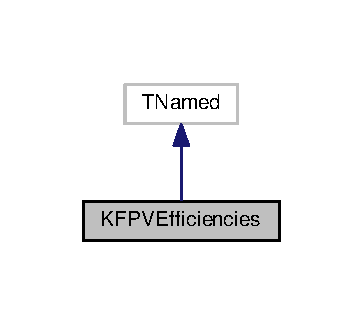
\includegraphics[width=174pt]{classKFPVEfficiencies__inherit__graph}
\end{center}
\end{figure}


Collaboration diagram for K\+F\+P\+V\+Efficiencies\+:
\nopagebreak
\begin{figure}[H]
\begin{center}
\leavevmode
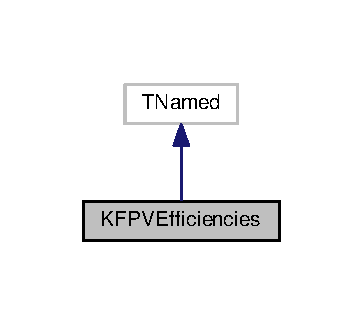
\includegraphics[width=174pt]{classKFPVEfficiencies__coll__graph}
\end{center}
\end{figure}
\subsection*{Public Member Functions}
\begin{DoxyCompactItemize}
\item 
virtual void \hyperlink{classKFPVEfficiencies_a6c8fe247dd32832b70f999da9620acb1}{Add\+Counter} (T\+String shortname, T\+String name)
\item 
\hyperlink{classKFPVEfficiencies}{K\+F\+P\+V\+Efficiencies} \& \hyperlink{classKFPVEfficiencies_ae3bf5a78152a2647602e4e8fc208e0cc}{operator+=} (\hyperlink{classKFPVEfficiencies}{K\+F\+P\+V\+Efficiencies} \&a)\hypertarget{classKFPVEfficiencies_ae3bf5a78152a2647602e4e8fc208e0cc}{}\label{classKFPVEfficiencies_ae3bf5a78152a2647602e4e8fc208e0cc}

\begin{DoxyCompactList}\small\item\em Operator to add efficiency table from object \char`\"{}a\char`\"{} to the current object. Returns the current object after addition. \end{DoxyCompactList}\item 
void \hyperlink{classKFPVEfficiencies_a70b97a29c9f82ee37c878727e8329984}{Calc\+Eff} ()\hypertarget{classKFPVEfficiencies_a70b97a29c9f82ee37c878727e8329984}{}\label{classKFPVEfficiencies_a70b97a29c9f82ee37c878727e8329984}

\begin{DoxyCompactList}\small\item\em Function to calculate efficiency after all counters are set. If the counters are modified the function should be called again. \end{DoxyCompactList}\item 
void \hyperlink{classKFPVEfficiencies_a331cde519b6ab92fbad094aeb682863b}{Inc} (bool is\+Reco, int n\+Clones, T\+String name)
\item 
void \hyperlink{classKFPVEfficiencies_aea0df6884f262e4dfebe3d07eb4c9b2e}{Inc\+Reco} (bool is\+Ghost, bool is\+Bg, T\+String name)
\item 
void \hyperlink{classKFPVEfficiencies_a0a56a067fb05669bdf7a74c8debbe0f7}{Print\+Eff} ()\hypertarget{classKFPVEfficiencies_a0a56a067fb05669bdf7a74c8debbe0f7}{}\label{classKFPVEfficiencies_a0a56a067fb05669bdf7a74c8debbe0f7}

\begin{DoxyCompactList}\small\item\em Prints the efficiency table on the screen. \end{DoxyCompactList}\item 
void \hyperlink{classKFPVEfficiencies_a70663999ca44fa5be5e92892940d2595}{Add\+From\+File} (T\+String file\+Name)\hypertarget{classKFPVEfficiencies_a70663999ca44fa5be5e92892940d2595}{}\label{classKFPVEfficiencies_a70663999ca44fa5be5e92892940d2595}

\begin{DoxyCompactList}\small\item\em Adds efficiency from the file with the name defined by \char`\"{}file\+Name\char`\"{} to the current objects. \end{DoxyCompactList}\end{DoxyCompactItemize}
\subsection*{Friends}
\begin{DoxyCompactItemize}
\item 
std\+::fstream \& \hyperlink{classKFPVEfficiencies_a8003529fc9ef679bed0c6c5732f13e6a}{operator$<$$<$} (std\+::fstream \&strm, \hyperlink{classKFPVEfficiencies}{K\+F\+P\+V\+Efficiencies} \&a)\hypertarget{classKFPVEfficiencies_a8003529fc9ef679bed0c6c5732f13e6a}{}\label{classKFPVEfficiencies_a8003529fc9ef679bed0c6c5732f13e6a}

\begin{DoxyCompactList}\small\item\em Operator to write efficiencies to file. \end{DoxyCompactList}\item 
std\+::fstream \& \hyperlink{classKFPVEfficiencies_a59a63eaec59e54dbeb5f96bbfb373c99}{operator$>$$>$} (std\+::fstream \&strm, \hyperlink{classKFPVEfficiencies}{K\+F\+P\+V\+Efficiencies} \&a)\hypertarget{classKFPVEfficiencies_a59a63eaec59e54dbeb5f96bbfb373c99}{}\label{classKFPVEfficiencies_a59a63eaec59e54dbeb5f96bbfb373c99}

\begin{DoxyCompactList}\small\item\em Operator to read efficiencies from file. \end{DoxyCompactList}\end{DoxyCompactItemize}


\subsection{Detailed Description}
Class to calculate efficiency of KF Particle Finder. 

\begin{DoxyAuthor}{Author}
M.\+Zyzak, I.\+Kisel 
\end{DoxyAuthor}
\begin{DoxyDate}{Date}
05.\+02.\+2019 
\end{DoxyDate}
\begin{DoxyVersion}{Version}
1.\+0
\end{DoxyVersion}
The class calculates reconstruction efficiency of the primary vertices.~\newline
Definitions\+:~\newline
background -\/ physics background, when daughter particle come from the secondary vertex;~\newline
ghost -\/ combinatorial background, tracks do not form a real vertex;~\newline
clone -\/ a vertex is reconstructed several times, for example, half of tracks form one group and another half form second group. 

\subsection{Member Function Documentation}
\index{K\+F\+P\+V\+Efficiencies@{K\+F\+P\+V\+Efficiencies}!Add\+Counter@{Add\+Counter}}
\index{Add\+Counter@{Add\+Counter}!K\+F\+P\+V\+Efficiencies@{K\+F\+P\+V\+Efficiencies}}
\subsubsection[{\texorpdfstring{Add\+Counter(\+T\+String shortname, T\+String name)}{AddCounter(TString shortname, TString name)}}]{\setlength{\rightskip}{0pt plus 5cm}virtual void K\+F\+P\+V\+Efficiencies\+::\+Add\+Counter (
\begin{DoxyParamCaption}
\item[{T\+String}]{shortname, }
\item[{T\+String}]{name}
\end{DoxyParamCaption}
)\hspace{0.3cm}{\ttfamily [inline]}, {\ttfamily [virtual]}}\hypertarget{classKFPVEfficiencies_a6c8fe247dd32832b70f999da9620acb1}{}\label{classKFPVEfficiencies_a6c8fe247dd32832b70f999da9620acb1}
Adds a counter with the name defined by \char`\"{}name\char`\"{} to all counter objects. For easiness of operation with counters, a shortname is assigned to each of them and the corresponding entry in the map indices is done. 
\begin{DoxyParams}[1]{Parameters}
\mbox{\tt in}  & {\em shortname} & -\/ a short name of the counter for fast and easy access to its index \\
\hline
\mbox{\tt in}  & {\em name} & -\/ name of the counter which is added to each counter object.\\
\hline
\end{DoxyParams}
\index{K\+F\+P\+V\+Efficiencies@{K\+F\+P\+V\+Efficiencies}!Inc@{Inc}}
\index{Inc@{Inc}!K\+F\+P\+V\+Efficiencies@{K\+F\+P\+V\+Efficiencies}}
\subsubsection[{\texorpdfstring{Inc(bool is\+Reco, int n\+Clones, T\+String name)}{Inc(bool isReco, int nClones, TString name)}}]{\setlength{\rightskip}{0pt plus 5cm}void K\+F\+P\+V\+Efficiencies\+::\+Inc (
\begin{DoxyParamCaption}
\item[{bool}]{is\+Reco, }
\item[{int}]{n\+Clones, }
\item[{T\+String}]{name}
\end{DoxyParamCaption}
)\hspace{0.3cm}{\ttfamily [inline]}}\hypertarget{classKFPVEfficiencies_a331cde519b6ab92fbad094aeb682863b}{}\label{classKFPVEfficiencies_a331cde519b6ab92fbad094aeb682863b}
Increases counters by one, if the corresponding boolean variable is \char`\"{}true\char`\"{}. MC counter is increased in any case. 
\begin{DoxyParams}[1]{Parameters}
\mbox{\tt in}  & {\em is\+Reco} & -\/ \char`\"{}true\char`\"{} if vertex is reconstructed \\
\hline
\mbox{\tt in}  & {\em n\+Clones} & -\/ number of double reconstructed vertices for the given MC vertex, will be added to the \char`\"{}clone\char`\"{} counters \\
\hline
\mbox{\tt in}  & {\em name} & -\/ \char`\"{}shortname\char`\"{} of the set of counters, which should be increased\\
\hline
\end{DoxyParams}
\index{K\+F\+P\+V\+Efficiencies@{K\+F\+P\+V\+Efficiencies}!Inc\+Reco@{Inc\+Reco}}
\index{Inc\+Reco@{Inc\+Reco}!K\+F\+P\+V\+Efficiencies@{K\+F\+P\+V\+Efficiencies}}
\subsubsection[{\texorpdfstring{Inc\+Reco(bool is\+Ghost, bool is\+Bg, T\+String name)}{IncReco(bool isGhost, bool isBg, TString name)}}]{\setlength{\rightskip}{0pt plus 5cm}void K\+F\+P\+V\+Efficiencies\+::\+Inc\+Reco (
\begin{DoxyParamCaption}
\item[{bool}]{is\+Ghost, }
\item[{bool}]{is\+Bg, }
\item[{T\+String}]{name}
\end{DoxyParamCaption}
)\hspace{0.3cm}{\ttfamily [inline]}}\hypertarget{classKFPVEfficiencies_aea0df6884f262e4dfebe3d07eb4c9b2e}{}\label{classKFPVEfficiencies_aea0df6884f262e4dfebe3d07eb4c9b2e}
Increases counters by one, if the corresponding boolean variable is \char`\"{}true\char`\"{}. 
\begin{DoxyParams}[1]{Parameters}
\mbox{\tt in}  & {\em is\+Ghost} & -\/ \char`\"{}true\char`\"{} if ghost is added \\
\hline
\mbox{\tt in}  & {\em is\+Bg} & -\/ \char`\"{}true\char`\"{} if physics background is added \\
\hline
\mbox{\tt in}  & {\em name} & -\/ \char`\"{}shortname\char`\"{} of the set of counters, which should be increased\\
\hline
\end{DoxyParams}


The documentation for this class was generated from the following file\+:\begin{DoxyCompactItemize}
\item 
/home/user/cbmdir/kfpf/\+K\+F\+Particle/\+K\+F\+Particle\+Performance/K\+F\+P\+V\+Efficiencies.\+h\end{DoxyCompactItemize}

\hypertarget{classKFPVertex}{}\section{K\+F\+P\+Vertex Class Reference}
\label{classKFPVertex}\index{K\+F\+P\+Vertex@{K\+F\+P\+Vertex}}


A scalar class for storage of the vertex in the cartesian parametrisation.  




{\ttfamily \#include $<$K\+F\+P\+Vertex.\+h$>$}

\subsection*{Public Member Functions}
\begin{DoxyCompactItemize}
\item 
float \hyperlink{classKFPVertex_a5a15225422c34336de1f89773182d389}{GetX} () const \hypertarget{classKFPVertex_a5a15225422c34336de1f89773182d389}{}\label{classKFPVertex_a5a15225422c34336de1f89773182d389}

\begin{DoxyCompactList}\small\item\em Returns X coordinate of the vertex. \end{DoxyCompactList}\item 
float \hyperlink{classKFPVertex_acdd00e757d57875e949329239894c78d}{GetY} () const \hypertarget{classKFPVertex_acdd00e757d57875e949329239894c78d}{}\label{classKFPVertex_acdd00e757d57875e949329239894c78d}

\begin{DoxyCompactList}\small\item\em Returns Y coordinate of the vertex. \end{DoxyCompactList}\item 
float \hyperlink{classKFPVertex_ae30ff55889db2e51bdfef446c730c7dd}{GetZ} () const \hypertarget{classKFPVertex_ae30ff55889db2e51bdfef446c730c7dd}{}\label{classKFPVertex_ae30ff55889db2e51bdfef446c730c7dd}

\begin{DoxyCompactList}\small\item\em Returns Z coordinate of the vertex. \end{DoxyCompactList}\item 
void \hyperlink{classKFPVertex_a32d248f48c1b29dc867a4133e835ae5c}{Get\+X\+YZ} (float $\ast$position) const 
\item 
void \hyperlink{classKFPVertex_afe5ec985311fa968cb673e6c6fea19b9}{Get\+X\+YZ} (double $\ast$position) const 
\item 
void \hyperlink{classKFPVertex_a53026f57dd31dc2e3f43783b89c84eea}{Get\+Covariance\+Matrix} (float $\ast$covmatrix) const 
\item 
void \hyperlink{classKFPVertex_a252f921b95faba943598230924c1ea6e}{Get\+Covariance\+Matrix} (double $\ast$covmatrix) const 
\item 
float \hyperlink{classKFPVertex_a2418610813ce90a9e8ab2eab946d5e57}{Get\+Chi2per\+N\+DF} () const \hypertarget{classKFPVertex_a2418610813ce90a9e8ab2eab946d5e57}{}\label{classKFPVertex_a2418610813ce90a9e8ab2eab946d5e57}

\begin{DoxyCompactList}\small\item\em Returns Chi2/\+N\+DF of the vertex, N\+DF is a number of degrees of freedom. \end{DoxyCompactList}\item 
float \hyperlink{classKFPVertex_a172744bf6e2a9a3bd4c5bfb2420acf77}{Get\+Chi2} () const \hypertarget{classKFPVertex_a172744bf6e2a9a3bd4c5bfb2420acf77}{}\label{classKFPVertex_a172744bf6e2a9a3bd4c5bfb2420acf77}

\begin{DoxyCompactList}\small\item\em Returns Chi2 of the vertex fit. \end{DoxyCompactList}\item 
int \hyperlink{classKFPVertex_a51e1f8df396bb4b05e5eb41d070b4a36}{Get\+N\+DF} () const \hypertarget{classKFPVertex_a51e1f8df396bb4b05e5eb41d070b4a36}{}\label{classKFPVertex_a51e1f8df396bb4b05e5eb41d070b4a36}

\begin{DoxyCompactList}\small\item\em Returns number of degrees of freedom of the vertex. \end{DoxyCompactList}\item 
int \hyperlink{classKFPVertex_a321dd26ba4bd5f3d62448df30585d326}{Get\+N\+Contributors} () const \hypertarget{classKFPVertex_a321dd26ba4bd5f3d62448df30585d326}{}\label{classKFPVertex_a321dd26ba4bd5f3d62448df30585d326}

\begin{DoxyCompactList}\small\item\em Returns number of tracks which were used for construction of the vertex. \end{DoxyCompactList}\item 
float \hyperlink{classKFPVertex_a9838b2b30d2b861522511abcb7179af4}{Get\+Parameter} (int i) const 
\begin{DoxyCompactList}\small\item\em Returns parameter \char`\"{}i\char`\"{} of the vertex. \end{DoxyCompactList}\item 
float \hyperlink{classKFPVertex_a871292a16c518a101587eb6afd034f4c}{Get\+Covariance} (int i) const 
\begin{DoxyCompactList}\small\item\em Returns element of the covariance matrix \char`\"{}i\char`\"{} of the vertex. \end{DoxyCompactList}\item 
void \hyperlink{classKFPVertex_a83b2d67398746613e079f20134209e22}{Set\+X\+YZ} (float $\ast$position)
\item 
void \hyperlink{classKFPVertex_a2f58a966b373d4ca82c99d3c0e063e61}{Set\+X\+YZ} (float x, float y, float z)
\item 
void \hyperlink{classKFPVertex_ac737d17f674d5beb4fd0598e5599a110}{SetX} (float x)\hypertarget{classKFPVertex_ac737d17f674d5beb4fd0598e5599a110}{}\label{classKFPVertex_ac737d17f674d5beb4fd0598e5599a110}

\begin{DoxyCompactList}\small\item\em Sets X coordinate of the vertex. \end{DoxyCompactList}\item 
void \hyperlink{classKFPVertex_a34d56e65dd85b71fe87e6557d28eeef1}{SetY} (float y)\hypertarget{classKFPVertex_a34d56e65dd85b71fe87e6557d28eeef1}{}\label{classKFPVertex_a34d56e65dd85b71fe87e6557d28eeef1}

\begin{DoxyCompactList}\small\item\em Sets Y coordinate of the vertex. \end{DoxyCompactList}\item 
void \hyperlink{classKFPVertex_a65646df4853da48bd589bf2337f33f54}{SetZ} (float z)\hypertarget{classKFPVertex_a65646df4853da48bd589bf2337f33f54}{}\label{classKFPVertex_a65646df4853da48bd589bf2337f33f54}

\begin{DoxyCompactList}\small\item\em Sets Z coordinate of the vertex. \end{DoxyCompactList}\item 
void \hyperlink{classKFPVertex_a6e29b8eb79de8f15cfd06c55a5c986e5}{Set\+Chi2} (float chi)\hypertarget{classKFPVertex_a6e29b8eb79de8f15cfd06c55a5c986e5}{}\label{classKFPVertex_a6e29b8eb79de8f15cfd06c55a5c986e5}

\begin{DoxyCompactList}\small\item\em Sets Chi2 of the vertex. \end{DoxyCompactList}\item 
void \hyperlink{classKFPVertex_a9e2bb0acbfc334ed211e629b73949531}{Set\+N\+DF} (int ndf)\hypertarget{classKFPVertex_a9e2bb0acbfc334ed211e629b73949531}{}\label{classKFPVertex_a9e2bb0acbfc334ed211e629b73949531}

\begin{DoxyCompactList}\small\item\em Sets number of degrees of freedom of the vertex. \end{DoxyCompactList}\item 
void \hyperlink{classKFPVertex_ae2f6ae77d3b159a19466e78892787684}{Set\+N\+Contributors} (int nc)\hypertarget{classKFPVertex_ae2f6ae77d3b159a19466e78892787684}{}\label{classKFPVertex_ae2f6ae77d3b159a19466e78892787684}

\begin{DoxyCompactList}\small\item\em Sets number of tracks which were used for construction of the vertex. \end{DoxyCompactList}\item 
void \hyperlink{classKFPVertex_acf653f4e9125ff6cfc16f51de2385b0c}{Set\+Covariance\+Matrix} (float $\ast$C)
\item 
void \hyperlink{classKFPVertex_a6f8f798968e437398172fab4e6a6e46b}{Set\+Covariance\+Matrix} (float C00, float C10, float C11, float C20, float C21, float C22)
\end{DoxyCompactItemize}


\subsection{Detailed Description}
A scalar class for storage of the vertex in the cartesian parametrisation. 

\begin{DoxyAuthor}{Author}
M.\+Zyzak, I.\+Kisel 
\end{DoxyAuthor}
\begin{DoxyDate}{Date}
05.\+02.\+2019 
\end{DoxyDate}
\begin{DoxyVersion}{Version}
1.\+0
\end{DoxyVersion}
A vertex is described with the state vector \{ X, Y, Z \} and the corresponding covariance matrix. Also contains chi2 of the fit, corresponding number of degrees of freedom, and number of tracks which were used to construct current vertex. The class is used to provide an external vertex through the interfaces to the KF Particle package. 

\subsection{Member Function Documentation}
\index{K\+F\+P\+Vertex@{K\+F\+P\+Vertex}!Get\+Covariance@{Get\+Covariance}}
\index{Get\+Covariance@{Get\+Covariance}!K\+F\+P\+Vertex@{K\+F\+P\+Vertex}}
\subsubsection[{\texorpdfstring{Get\+Covariance(int i) const }{GetCovariance(int i) const }}]{\setlength{\rightskip}{0pt plus 5cm}float K\+F\+P\+Vertex\+::\+Get\+Covariance (
\begin{DoxyParamCaption}
\item[{int}]{i}
\end{DoxyParamCaption}
) const\hspace{0.3cm}{\ttfamily [inline]}}\hypertarget{classKFPVertex_a871292a16c518a101587eb6afd034f4c}{}\label{classKFPVertex_a871292a16c518a101587eb6afd034f4c}


Returns element of the covariance matrix \char`\"{}i\char`\"{} of the vertex. 


\begin{DoxyParams}[1]{Parameters}
\mbox{\tt in}  & {\em i} & -\/ index of the element to be returned \\
\hline
\end{DoxyParams}
\index{K\+F\+P\+Vertex@{K\+F\+P\+Vertex}!Get\+Covariance\+Matrix@{Get\+Covariance\+Matrix}}
\index{Get\+Covariance\+Matrix@{Get\+Covariance\+Matrix}!K\+F\+P\+Vertex@{K\+F\+P\+Vertex}}
\subsubsection[{\texorpdfstring{Get\+Covariance\+Matrix(float $\ast$covmatrix) const }{GetCovarianceMatrix(float *covmatrix) const }}]{\setlength{\rightskip}{0pt plus 5cm}void K\+F\+P\+Vertex\+::\+Get\+Covariance\+Matrix (
\begin{DoxyParamCaption}
\item[{float $\ast$}]{covmatrix}
\end{DoxyParamCaption}
) const\hspace{0.3cm}{\ttfamily [inline]}}\hypertarget{classKFPVertex_a53026f57dd31dc2e3f43783b89c84eea}{}\label{classKFPVertex_a53026f57dd31dc2e3f43783b89c84eea}
Copies the covariance matrix of the vertex to the array of floats. 
\begin{DoxyParams}[1]{Parameters}
\mbox{\tt out}  & {\em covmatrix\mbox{[}6\mbox{]}} & -\/ the output array, where the covariance matrix is copied\\
\hline
\end{DoxyParams}
\index{K\+F\+P\+Vertex@{K\+F\+P\+Vertex}!Get\+Covariance\+Matrix@{Get\+Covariance\+Matrix}}
\index{Get\+Covariance\+Matrix@{Get\+Covariance\+Matrix}!K\+F\+P\+Vertex@{K\+F\+P\+Vertex}}
\subsubsection[{\texorpdfstring{Get\+Covariance\+Matrix(double $\ast$covmatrix) const }{GetCovarianceMatrix(double *covmatrix) const }}]{\setlength{\rightskip}{0pt plus 5cm}void K\+F\+P\+Vertex\+::\+Get\+Covariance\+Matrix (
\begin{DoxyParamCaption}
\item[{double $\ast$}]{covmatrix}
\end{DoxyParamCaption}
) const\hspace{0.3cm}{\ttfamily [inline]}}\hypertarget{classKFPVertex_a252f921b95faba943598230924c1ea6e}{}\label{classKFPVertex_a252f921b95faba943598230924c1ea6e}
Copies the covariance matrix of the vertex to the array of doubles. 
\begin{DoxyParams}[1]{Parameters}
\mbox{\tt out}  & {\em covmatrix\mbox{[}6\mbox{]}} & -\/ the output array, where the covariance matrix is copied\\
\hline
\end{DoxyParams}
\index{K\+F\+P\+Vertex@{K\+F\+P\+Vertex}!Get\+Parameter@{Get\+Parameter}}
\index{Get\+Parameter@{Get\+Parameter}!K\+F\+P\+Vertex@{K\+F\+P\+Vertex}}
\subsubsection[{\texorpdfstring{Get\+Parameter(int i) const }{GetParameter(int i) const }}]{\setlength{\rightskip}{0pt plus 5cm}float K\+F\+P\+Vertex\+::\+Get\+Parameter (
\begin{DoxyParamCaption}
\item[{int}]{i}
\end{DoxyParamCaption}
) const\hspace{0.3cm}{\ttfamily [inline]}}\hypertarget{classKFPVertex_a9838b2b30d2b861522511abcb7179af4}{}\label{classKFPVertex_a9838b2b30d2b861522511abcb7179af4}


Returns parameter \char`\"{}i\char`\"{} of the vertex. 


\begin{DoxyParams}[1]{Parameters}
\mbox{\tt in}  & {\em i} & -\/ index of the parameter to be returned \\
\hline
\end{DoxyParams}
\index{K\+F\+P\+Vertex@{K\+F\+P\+Vertex}!Get\+X\+YZ@{Get\+X\+YZ}}
\index{Get\+X\+YZ@{Get\+X\+YZ}!K\+F\+P\+Vertex@{K\+F\+P\+Vertex}}
\subsubsection[{\texorpdfstring{Get\+X\+Y\+Z(float $\ast$position) const }{GetXYZ(float *position) const }}]{\setlength{\rightskip}{0pt plus 5cm}void K\+F\+P\+Vertex\+::\+Get\+X\+YZ (
\begin{DoxyParamCaption}
\item[{float $\ast$}]{position}
\end{DoxyParamCaption}
) const\hspace{0.3cm}{\ttfamily [inline]}}\hypertarget{classKFPVertex_a32d248f48c1b29dc867a4133e835ae5c}{}\label{classKFPVertex_a32d248f48c1b29dc867a4133e835ae5c}
Copies position of the vertex to the output array of floats. 
\begin{DoxyParams}[1]{Parameters}
\mbox{\tt out}  & {\em position} & -\/ the output array with the position of the vertex \\
\hline
\end{DoxyParams}
\index{K\+F\+P\+Vertex@{K\+F\+P\+Vertex}!Get\+X\+YZ@{Get\+X\+YZ}}
\index{Get\+X\+YZ@{Get\+X\+YZ}!K\+F\+P\+Vertex@{K\+F\+P\+Vertex}}
\subsubsection[{\texorpdfstring{Get\+X\+Y\+Z(double $\ast$position) const }{GetXYZ(double *position) const }}]{\setlength{\rightskip}{0pt plus 5cm}void K\+F\+P\+Vertex\+::\+Get\+X\+YZ (
\begin{DoxyParamCaption}
\item[{double $\ast$}]{position}
\end{DoxyParamCaption}
) const\hspace{0.3cm}{\ttfamily [inline]}}\hypertarget{classKFPVertex_afe5ec985311fa968cb673e6c6fea19b9}{}\label{classKFPVertex_afe5ec985311fa968cb673e6c6fea19b9}
Copies position of the vertex to the output array of doubles. 
\begin{DoxyParams}[1]{Parameters}
\mbox{\tt out}  & {\em position} & -\/ the output array with the position of the vertex \\
\hline
\end{DoxyParams}
\index{K\+F\+P\+Vertex@{K\+F\+P\+Vertex}!Set\+Covariance\+Matrix@{Set\+Covariance\+Matrix}}
\index{Set\+Covariance\+Matrix@{Set\+Covariance\+Matrix}!K\+F\+P\+Vertex@{K\+F\+P\+Vertex}}
\subsubsection[{\texorpdfstring{Set\+Covariance\+Matrix(float $\ast$\+C)}{SetCovarianceMatrix(float *C)}}]{\setlength{\rightskip}{0pt plus 5cm}void K\+F\+P\+Vertex\+::\+Set\+Covariance\+Matrix (
\begin{DoxyParamCaption}
\item[{float $\ast$}]{C}
\end{DoxyParamCaption}
)\hspace{0.3cm}{\ttfamily [inline]}}\hypertarget{classKFPVertex_acf653f4e9125ff6cfc16f51de2385b0c}{}\label{classKFPVertex_acf653f4e9125ff6cfc16f51de2385b0c}
Sets the covariance matrix from the input array of floats. 
\begin{DoxyParams}[1]{Parameters}
\mbox{\tt in}  & {\em C\mbox{[}6\mbox{]}} & -\/ array with the input elements of the covariance matrix stored in the lower triangular form\\
\hline
\end{DoxyParams}
\index{K\+F\+P\+Vertex@{K\+F\+P\+Vertex}!Set\+Covariance\+Matrix@{Set\+Covariance\+Matrix}}
\index{Set\+Covariance\+Matrix@{Set\+Covariance\+Matrix}!K\+F\+P\+Vertex@{K\+F\+P\+Vertex}}
\subsubsection[{\texorpdfstring{Set\+Covariance\+Matrix(float C00, float C10, float C11, float C20, float C21, float C22)}{SetCovarianceMatrix(float C00, float C10, float C11, float C20, float C21, float C22)}}]{\setlength{\rightskip}{0pt plus 5cm}void K\+F\+P\+Vertex\+::\+Set\+Covariance\+Matrix (
\begin{DoxyParamCaption}
\item[{float}]{C00, }
\item[{float}]{C10, }
\item[{float}]{C11, }
\item[{float}]{C20, }
\item[{float}]{C21, }
\item[{float}]{C22}
\end{DoxyParamCaption}
)\hspace{0.3cm}{\ttfamily [inline]}}\hypertarget{classKFPVertex_a6f8f798968e437398172fab4e6a6e46b}{}\label{classKFPVertex_a6f8f798968e437398172fab4e6a6e46b}
Sets the covariance matrix from the input array of floats. 
\begin{DoxyParams}[1]{Parameters}
\mbox{\tt in}  & {\em C00} & -\/ Cxx \\
\hline
\mbox{\tt in}  & {\em C10} & -\/ Cxy = Cyx \\
\hline
\mbox{\tt in}  & {\em C11} & -\/ Cyy \\
\hline
\mbox{\tt in}  & {\em C20} & -\/ Cxz = Czx \\
\hline
\mbox{\tt in}  & {\em C21} & -\/ Cyz = Czy \\
\hline
\mbox{\tt in}  & {\em C22} & -\/ Czz\\
\hline
\end{DoxyParams}
\index{K\+F\+P\+Vertex@{K\+F\+P\+Vertex}!Set\+X\+YZ@{Set\+X\+YZ}}
\index{Set\+X\+YZ@{Set\+X\+YZ}!K\+F\+P\+Vertex@{K\+F\+P\+Vertex}}
\subsubsection[{\texorpdfstring{Set\+X\+Y\+Z(float $\ast$position)}{SetXYZ(float *position)}}]{\setlength{\rightskip}{0pt plus 5cm}void K\+F\+P\+Vertex\+::\+Set\+X\+YZ (
\begin{DoxyParamCaption}
\item[{float $\ast$}]{position}
\end{DoxyParamCaption}
)\hspace{0.3cm}{\ttfamily [inline]}}\hypertarget{classKFPVertex_a83b2d67398746613e079f20134209e22}{}\label{classKFPVertex_a83b2d67398746613e079f20134209e22}
Sets position \{ X, Y, Z \} of the vertex from the input array of doubles. 
\begin{DoxyParams}[1]{Parameters}
\mbox{\tt in}  & {\em position} & -\/ input array with the vertex parameters \\
\hline
\end{DoxyParams}
\index{K\+F\+P\+Vertex@{K\+F\+P\+Vertex}!Set\+X\+YZ@{Set\+X\+YZ}}
\index{Set\+X\+YZ@{Set\+X\+YZ}!K\+F\+P\+Vertex@{K\+F\+P\+Vertex}}
\subsubsection[{\texorpdfstring{Set\+X\+Y\+Z(float x, float y, float z)}{SetXYZ(float x, float y, float z)}}]{\setlength{\rightskip}{0pt plus 5cm}void K\+F\+P\+Vertex\+::\+Set\+X\+YZ (
\begin{DoxyParamCaption}
\item[{float}]{x, }
\item[{float}]{y, }
\item[{float}]{z}
\end{DoxyParamCaption}
)\hspace{0.3cm}{\ttfamily [inline]}}\hypertarget{classKFPVertex_a2f58a966b373d4ca82c99d3c0e063e61}{}\label{classKFPVertex_a2f58a966b373d4ca82c99d3c0e063e61}
Sets position \{ X, Y, Z \} of the vertex. 
\begin{DoxyParams}[1]{Parameters}
\mbox{\tt in}  & {\em x} & -\/ X coordinate to be set \\
\hline
\mbox{\tt in}  & {\em y} & -\/ Y coordinate to be set \\
\hline
\mbox{\tt in}  & {\em z} & -\/ Z coordinate to be set \\
\hline
\end{DoxyParams}


The documentation for this class was generated from the following files\+:\begin{DoxyCompactItemize}
\item 
/home/user/cbmdir/kfpf/\+K\+F\+Particle/\+K\+F\+Particle/K\+F\+P\+Vertex.\+h\item 
/home/user/cbmdir/kfpf/\+K\+F\+Particle/\+K\+F\+Particle/K\+F\+P\+Vertex.\+cxx\end{DoxyCompactItemize}

\hypertarget{classKFVertex}{}\section{K\+F\+Vertex Class Reference}
\label{classKFVertex}\index{K\+F\+Vertex@{K\+F\+Vertex}}


Mathematics for reconstruction of primary vertices based on \hyperlink{classKFParticle}{K\+F\+Particle}.  




{\ttfamily \#include $<$K\+F\+Vertex.\+h$>$}



Inheritance diagram for K\+F\+Vertex\+:\nopagebreak
\begin{figure}[H]
\begin{center}
\leavevmode
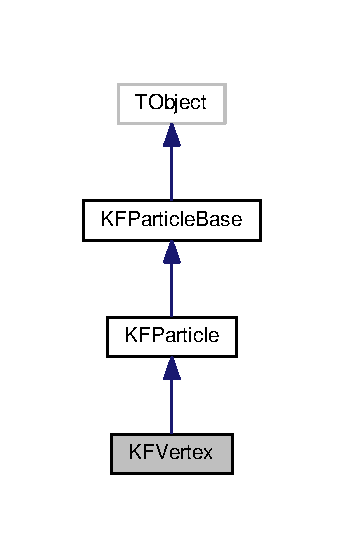
\includegraphics[width=165pt]{classKFVertex__inherit__graph}
\end{center}
\end{figure}


Collaboration diagram for K\+F\+Vertex\+:\nopagebreak
\begin{figure}[H]
\begin{center}
\leavevmode
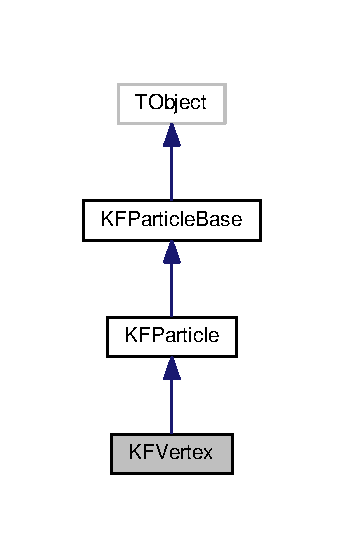
\includegraphics[width=165pt]{classKFVertex__coll__graph}
\end{center}
\end{figure}
\subsection*{Public Member Functions}
\begin{DoxyCompactItemize}
\item 
\hyperlink{classKFVertex_ab591c46e3f20b9f4c1d39207d7127e59}{K\+F\+Vertex} (const \hyperlink{classKFParticle}{K\+F\+Particle} \&particle)\hypertarget{classKFVertex_ab591c46e3f20b9f4c1d39207d7127e59}{}\label{classKFVertex_ab591c46e3f20b9f4c1d39207d7127e59}

\begin{DoxyCompactList}\small\item\em Vertex is constructed from the current position of a given particle. \end{DoxyCompactList}\item 
\hyperlink{classKFVertex_add291171f94e133f9a197659d395eb7b}{K\+F\+Vertex} (const \hyperlink{classKFPVertex}{K\+F\+P\+Vertex} \&vertex)
\item 
Int\+\_\+t \hyperlink{classKFVertex_a0a51761dbb09cf89357b1a19cf2df139}{Get\+N\+Contributors} () const \hypertarget{classKFVertex_a0a51761dbb09cf89357b1a19cf2df139}{}\label{classKFVertex_a0a51761dbb09cf89357b1a19cf2df139}

\begin{DoxyCompactList}\small\item\em Returns number of particles used for construction of the vertex. \end{DoxyCompactList}\item 
void \hyperlink{classKFVertex_a33c09d3c2321086ff9564199425d0918}{operator+=} (const \hyperlink{classKFParticle}{K\+F\+Particle} \&Daughter)\hypertarget{classKFVertex_a33c09d3c2321086ff9564199425d0918}{}\label{classKFVertex_a33c09d3c2321086ff9564199425d0918}

\begin{DoxyCompactList}\small\item\em Adds particle to a vertex. \end{DoxyCompactList}\item 
\hyperlink{classKFVertex}{K\+F\+Vertex} \hyperlink{classKFVertex_aa7bf314d94f6d9b5ba7a734bd0e7db1c}{operator-\/} (const \hyperlink{classKFParticle}{K\+F\+Particle} \&Daughter) const \hypertarget{classKFVertex_aa7bf314d94f6d9b5ba7a734bd0e7db1c}{}\label{classKFVertex_aa7bf314d94f6d9b5ba7a734bd0e7db1c}

\begin{DoxyCompactList}\small\item\em Subtracts particle from a vertex, returns temporary object. Initial vertex stays untouched. \end{DoxyCompactList}\item 
void \hyperlink{classKFVertex_aa196e7fe7d77847e7684e26d158bc16c}{operator-\/=} (const \hyperlink{classKFParticle}{K\+F\+Particle} \&Daughter)\hypertarget{classKFVertex_aa196e7fe7d77847e7684e26d158bc16c}{}\label{classKFVertex_aa196e7fe7d77847e7684e26d158bc16c}

\begin{DoxyCompactList}\small\item\em Subtracts particle from a current vertex. \end{DoxyCompactList}\item 
void \hyperlink{classKFVertex_a7b38221467e21270dd68cc3d7928393c}{Set\+Beam\+Constraint} (float \hyperlink{classKFParticleBase_af624ef17e57f675476a2a0e597ce2983}{X}, float \hyperlink{classKFParticleBase_ad7d7e1a209955c43efac37d6136ac406}{Y}, float \hyperlink{classKFParticleBase_a96e631c939d83ff67c82701ed8255200}{Z}, float ErrX, float ErrY, float ErrZ)
\item 
void \hyperlink{classKFVertex_a5e50ebe906e13c95e6bde55668a35565}{Set\+Beam\+Constraint\+Off} ()
\item 
void \hyperlink{classKFVertex_a0398208d64532d964a2c6c4c061c349c}{Construct\+Primary\+Vertex} (const \hyperlink{classKFParticle}{K\+F\+Particle} $\ast$v\+Daughters\mbox{[}$\,$\mbox{]}, int n\+Daughters, Bool\+\_\+t vtx\+Flag\mbox{[}$\,$\mbox{]}, float Chi\+Cut=3.\+5)
\end{DoxyCompactItemize}
\subsection*{Protected Attributes}
\begin{DoxyCompactItemize}
\item 
Bool\+\_\+t \hyperlink{classKFVertex_a5da11170d128a3adf9a0f2f672694b9e}{f\+Is\+Constrained}\hypertarget{classKFVertex_a5da11170d128a3adf9a0f2f672694b9e}{}\label{classKFVertex_a5da11170d128a3adf9a0f2f672694b9e}

\begin{DoxyCompactList}\small\item\em Flag showing if the the beam constraint is set. \end{DoxyCompactList}\end{DoxyCompactItemize}
\subsection*{Additional Inherited Members}


\subsection{Detailed Description}
Mathematics for reconstruction of primary vertices based on \hyperlink{classKFParticle}{K\+F\+Particle}. 

\begin{DoxyAuthor}{Author}
S.\+Gorbunov, I.\+Kisel, M.\+Zyzak 
\end{DoxyAuthor}
\begin{DoxyDate}{Date}
05.\+02.\+2019 
\end{DoxyDate}
\begin{DoxyVersion}{Version}
1.\+0
\end{DoxyVersion}
The class is inherited from \hyperlink{classKFParticle}{K\+F\+Particle}, adds functionality for reconstruction of primary vertices. 

\subsection{Constructor \& Destructor Documentation}
\index{K\+F\+Vertex@{K\+F\+Vertex}!K\+F\+Vertex@{K\+F\+Vertex}}
\index{K\+F\+Vertex@{K\+F\+Vertex}!K\+F\+Vertex@{K\+F\+Vertex}}
\subsubsection[{\texorpdfstring{K\+F\+Vertex(const K\+F\+P\+Vertex \&vertex)}{KFVertex(const KFPVertex &vertex)}}]{\setlength{\rightskip}{0pt plus 5cm}K\+F\+Vertex\+::\+K\+F\+Vertex (
\begin{DoxyParamCaption}
\item[{const {\bf K\+F\+P\+Vertex} \&}]{vertex}
\end{DoxyParamCaption}
)}\hypertarget{classKFVertex_add291171f94e133f9a197659d395eb7b}{}\label{classKFVertex_add291171f94e133f9a197659d395eb7b}
Constructor from \hyperlink{classKFPVertex}{K\+F\+P\+Vertex}. 

\subsection{Member Function Documentation}
\index{K\+F\+Vertex@{K\+F\+Vertex}!Construct\+Primary\+Vertex@{Construct\+Primary\+Vertex}}
\index{Construct\+Primary\+Vertex@{Construct\+Primary\+Vertex}!K\+F\+Vertex@{K\+F\+Vertex}}
\subsubsection[{\texorpdfstring{Construct\+Primary\+Vertex(const K\+F\+Particle $\ast$v\+Daughters[], int n\+Daughters, Bool\+\_\+t vtx\+Flag[], float Chi\+Cut=3.\+5)}{ConstructPrimaryVertex(const KFParticle *vDaughters[], int nDaughters, Bool_t vtxFlag[], float ChiCut=3.5)}}]{\setlength{\rightskip}{0pt plus 5cm}void K\+F\+Vertex\+::\+Construct\+Primary\+Vertex (
\begin{DoxyParamCaption}
\item[{const {\bf K\+F\+Particle} $\ast$}]{v\+Daughters\mbox{[}$\,$\mbox{]}, }
\item[{int}]{n\+Daughters, }
\item[{Bool\+\_\+t}]{vtx\+Flag\mbox{[}$\,$\mbox{]}, }
\item[{float}]{Chi\+Cut = {\ttfamily 3.5}}
\end{DoxyParamCaption}
)}\hypertarget{classKFVertex_a0398208d64532d964a2c6c4c061c349c}{}\label{classKFVertex_a0398208d64532d964a2c6c4c061c349c}
Reconstructs the primary vertex from a set of particles. Reconstruction is parformed in three steps\+:~\newline
1) vertex seed is constructed from all particles; ~\newline
2) if particle deviates more then on the \char`\"{}\+Chi\+Cut\char`\"{} it is rejected; ~\newline
3) the final vertex is constructed from the set of remaining particles.~\newline
Rejected particles are marked with \char`\"{}false\char`\"{} in the output array of flags. 
\begin{DoxyParams}[1]{Parameters}
\mbox{\tt in}  & {\em v\+Daughters} & -\/ input array of pointers to the particles \\
\hline
\mbox{\tt in}  & {\em n\+Daughters} & -\/ number of particles in the input array \\
\hline
\mbox{\tt out}  & {\em vtx\+Flag} & -\/ array of flags showing if particle was used in the vertex fit, if yes -\/ set to \char`\"{}true\char`\"{} \\
\hline
\mbox{\tt in}  & {\em Chi\+Cut} & -\/ cut on the chi2-\/deviation of the particle from the created seed, by default the cut is set to 3.\+5\\
\hline
\end{DoxyParams}
\index{K\+F\+Vertex@{K\+F\+Vertex}!Set\+Beam\+Constraint@{Set\+Beam\+Constraint}}
\index{Set\+Beam\+Constraint@{Set\+Beam\+Constraint}!K\+F\+Vertex@{K\+F\+Vertex}}
\subsubsection[{\texorpdfstring{Set\+Beam\+Constraint(float X, float Y, float Z, float Err\+X, float Err\+Y, float Err\+Z)}{SetBeamConstraint(float X, float Y, float Z, float ErrX, float ErrY, float ErrZ)}}]{\setlength{\rightskip}{0pt plus 5cm}void K\+F\+Vertex\+::\+Set\+Beam\+Constraint (
\begin{DoxyParamCaption}
\item[{float}]{X, }
\item[{float}]{Y, }
\item[{float}]{Z, }
\item[{float}]{ErrX, }
\item[{float}]{ErrY, }
\item[{float}]{ErrZ}
\end{DoxyParamCaption}
)}\hypertarget{classKFVertex_a7b38221467e21270dd68cc3d7928393c}{}\label{classKFVertex_a7b38221467e21270dd68cc3d7928393c}
Sets a soft beam constraint on the vertex position. 
\begin{DoxyParams}[1]{Parameters}
\mbox{\tt in}  & {\em x,y,z} & -\/ coordinates of the constraint \\
\hline
\mbox{\tt in}  & {\em errX,errY,errZ} & -\/ corresponding errors\\
\hline
\end{DoxyParams}
\index{K\+F\+Vertex@{K\+F\+Vertex}!Set\+Beam\+Constraint\+Off@{Set\+Beam\+Constraint\+Off}}
\index{Set\+Beam\+Constraint\+Off@{Set\+Beam\+Constraint\+Off}!K\+F\+Vertex@{K\+F\+Vertex}}
\subsubsection[{\texorpdfstring{Set\+Beam\+Constraint\+Off()}{SetBeamConstraintOff()}}]{\setlength{\rightskip}{0pt plus 5cm}void K\+F\+Vertex\+::\+Set\+Beam\+Constraint\+Off (
\begin{DoxyParamCaption}
{}
\end{DoxyParamCaption}
)}\hypertarget{classKFVertex_a5e50ebe906e13c95e6bde55668a35565}{}\label{classKFVertex_a5e50ebe906e13c95e6bde55668a35565}
Switches off the constraint. Should be called before \hyperlink{classKFVertex_a0398208d64532d964a2c6c4c061c349c}{K\+F\+Vertex\+::\+Construct\+Primary\+Vertex()} 

The documentation for this class was generated from the following files\+:\begin{DoxyCompactItemize}
\item 
/home/user/cbmdir/kfpf/\+K\+F\+Particle/\+K\+F\+Particle/K\+F\+Vertex.\+h\item 
/home/user/cbmdir/kfpf/\+K\+F\+Particle/\+K\+F\+Particle/K\+F\+Vertex.\+cxx\end{DoxyCompactItemize}

\hypertarget{classOutputContainer}{}\section{Output\+Container Class Reference}
\label{classOutputContainer}\index{Output\+Container@{Output\+Container}}


Container with output information about reconstructed particles and geometrical decay parameters (quantities to be cut in order to select particles)  




{\ttfamily \#include $<$Output\+Container.\+h$>$}



Collaboration diagram for Output\+Container\+:
\nopagebreak
\begin{figure}[H]
\begin{center}
\leavevmode
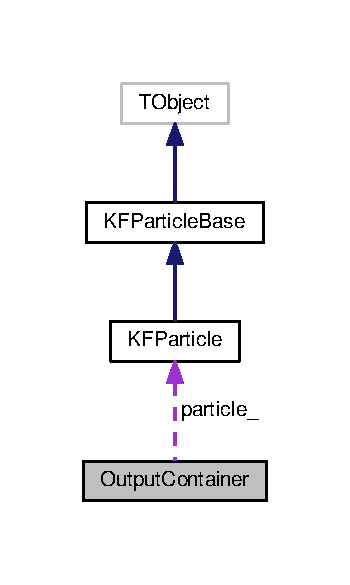
\includegraphics[width=168pt]{classOutputContainer__coll__graph}
\end{center}
\end{figure}
\subsection*{Public Member Functions}
\begin{DoxyCompactItemize}
\item 
void {\bfseries Set\+Chi2\+Prim\+Pos} (float value)\hypertarget{classOutputContainer_ac4d391c8d0e0829b7fe98139d69d1c34}{}\label{classOutputContainer_ac4d391c8d0e0829b7fe98139d69d1c34}

\item 
void {\bfseries Set\+Chi2\+Prim\+Neg} (float value)\hypertarget{classOutputContainer_a7aa4aed0887a86310051de07d69b6e3d}{}\label{classOutputContainer_a7aa4aed0887a86310051de07d69b6e3d}

\item 
void {\bfseries Set\+Distance} (float value)\hypertarget{classOutputContainer_a099e2cd16afcf680eaaff61d5b4bb53f}{}\label{classOutputContainer_a099e2cd16afcf680eaaff61d5b4bb53f}

\item 
void {\bfseries Set\+Cosine\+Daughter\+Pos} (float value)\hypertarget{classOutputContainer_aed510ed8aee7697d492d1ecf74fc5712}{}\label{classOutputContainer_aed510ed8aee7697d492d1ecf74fc5712}

\item 
void {\bfseries Set\+Cosine\+Daughter\+Neg} (float value)\hypertarget{classOutputContainer_a993a441de2b692e0de01356d91a0778c}{}\label{classOutputContainer_a993a441de2b692e0de01356d91a0778c}

\item 
void {\bfseries Set\+Chi2\+Geo} (float value)\hypertarget{classOutputContainer_a8d9a1efd7061a91e5f3378ba76d32907}{}\label{classOutputContainer_a8d9a1efd7061a91e5f3378ba76d32907}

\item 
void {\bfseries SetL} (float value)\hypertarget{classOutputContainer_a62c277b1b9e522d2f1d2e794ae391fd7}{}\label{classOutputContainer_a62c277b1b9e522d2f1d2e794ae391fd7}

\item 
void {\bfseries Set\+LdL} (float value)\hypertarget{classOutputContainer_a26c4eb14351d27e738c93ef545db5926}{}\label{classOutputContainer_a26c4eb14351d27e738c93ef545db5926}

\item 
void {\bfseries Set\+Is\+From\+PV} (int value)\hypertarget{classOutputContainer_a05c849ca8032917d4b70bd751b2bf9ef}{}\label{classOutputContainer_a05c849ca8032917d4b70bd751b2bf9ef}

\item 
void {\bfseries Set\+Cosine\+Topo} (float value)\hypertarget{classOutputContainer_a02b55dd31093252161c534de71081f08}{}\label{classOutputContainer_a02b55dd31093252161c534de71081f08}

\item 
void {\bfseries Set\+Sigma\+Mass\+Ratio} (float value)\hypertarget{classOutputContainer_a40aac1b715ddfae22116cf90063a5820}{}\label{classOutputContainer_a40aac1b715ddfae22116cf90063a5820}

\item 
void {\bfseries Set\+Chi2\+Topo} (float value)\hypertarget{classOutputContainer_aee3f737f8c982731e74dbfff6095fb9b}{}\label{classOutputContainer_aee3f737f8c982731e74dbfff6095fb9b}

\item 
void {\bfseries Set\+Particle} (\hyperlink{classKFParticle}{K\+F\+Particle} particle)\hypertarget{classOutputContainer_ae18ea1acbb871cc3fb57e59203641c56}{}\label{classOutputContainer_ae18ea1acbb871cc3fb57e59203641c56}

\item 
float {\bfseries Get\+Chi2\+Prim\+Pos} () const \hypertarget{classOutputContainer_a8b209257655e51302cf819344d76fd0e}{}\label{classOutputContainer_a8b209257655e51302cf819344d76fd0e}

\item 
float {\bfseries Get\+Chi2\+Prim\+Neg} () const \hypertarget{classOutputContainer_a15f9ed3f9e5f9f1ac20136ae4bb93410}{}\label{classOutputContainer_a15f9ed3f9e5f9f1ac20136ae4bb93410}

\item 
float {\bfseries Get\+Distance} () const \hypertarget{classOutputContainer_a4840fce251a629d4a3d16cf1387e75c1}{}\label{classOutputContainer_a4840fce251a629d4a3d16cf1387e75c1}

\item 
float {\bfseries Get\+Cosine\+Daughter\+Pos} () const \hypertarget{classOutputContainer_a775de6574434538d5808c570032b0dbe}{}\label{classOutputContainer_a775de6574434538d5808c570032b0dbe}

\item 
float {\bfseries Get\+Cosine\+Daughter\+Neg} () const \hypertarget{classOutputContainer_a2753890d24860c5007ae4887f4f2b9f8}{}\label{classOutputContainer_a2753890d24860c5007ae4887f4f2b9f8}

\item 
float {\bfseries Get\+Chi2\+Geo} () const \hypertarget{classOutputContainer_aeb5adf6ee71b602d42dd22bbf102701d}{}\label{classOutputContainer_aeb5adf6ee71b602d42dd22bbf102701d}

\item 
float {\bfseries GetL} () const \hypertarget{classOutputContainer_a2704034d20699d8ab82b35ed05d01582}{}\label{classOutputContainer_a2704034d20699d8ab82b35ed05d01582}

\item 
float {\bfseries Get\+LdL} () const \hypertarget{classOutputContainer_a1792d2a3d2227ab581cb0ab6f236d163}{}\label{classOutputContainer_a1792d2a3d2227ab581cb0ab6f236d163}

\item 
int {\bfseries Get\+Is\+From\+PV} () const \hypertarget{classOutputContainer_a675cc15e5d6fc530586d932c14bf33e3}{}\label{classOutputContainer_a675cc15e5d6fc530586d932c14bf33e3}

\item 
float {\bfseries Get\+Cosine\+Topo} () const \hypertarget{classOutputContainer_a640c56874891f7151a31186cd4ddc3ab}{}\label{classOutputContainer_a640c56874891f7151a31186cd4ddc3ab}

\item 
float {\bfseries Get\+Sigma\+Mass\+Ratio} () const \hypertarget{classOutputContainer_abd4758713cbbdaa67504818649a3bdad}{}\label{classOutputContainer_abd4758713cbbdaa67504818649a3bdad}

\item 
float {\bfseries Get\+Chi2\+Topo} () const \hypertarget{classOutputContainer_aecff1d4324266c05fcaf73807ca83201}{}\label{classOutputContainer_aecff1d4324266c05fcaf73807ca83201}

\item 
const \hyperlink{classKFParticle}{K\+F\+Particle} \& {\bfseries Get\+Particle} () const \hypertarget{classOutputContainer_a840a5cb5a08d726f22e8118b8306ac4f}{}\label{classOutputContainer_a840a5cb5a08d726f22e8118b8306ac4f}

\end{DoxyCompactItemize}
\subsection*{Protected Attributes}
\begin{DoxyCompactItemize}
\item 
float \hyperlink{classOutputContainer_aa382f97a717ece6c6d6ed6d34a4662d5}{chi2\+\_\+prim\+\_\+pos\+\_\+} \{-\/1.\}\hypertarget{classOutputContainer_aa382f97a717ece6c6d6ed6d34a4662d5}{}\label{classOutputContainer_aa382f97a717ece6c6d6ed6d34a4662d5}

\begin{DoxyCompactList}\small\item\em $\chi^2$ of the positive track to the primary vertex (PV) \end{DoxyCompactList}\item 
float \hyperlink{classOutputContainer_a20fe4406dabdd8400eb854476893d50e}{chi2\+\_\+prim\+\_\+neg\+\_\+} \{-\/1.\}\hypertarget{classOutputContainer_a20fe4406dabdd8400eb854476893d50e}{}\label{classOutputContainer_a20fe4406dabdd8400eb854476893d50e}

\begin{DoxyCompactList}\small\item\em $\chi^2$ of the negative track to the PV \end{DoxyCompactList}\item 
float \hyperlink{classOutputContainer_a118c01c668f399160b03505dc72e2681}{distance\+\_\+} \{-\/1.\}\hypertarget{classOutputContainer_a118c01c668f399160b03505dc72e2681}{}\label{classOutputContainer_a118c01c668f399160b03505dc72e2681}

\begin{DoxyCompactList}\small\item\em Distance between daughter tracks in their closest approach. \end{DoxyCompactList}\item 
float \hyperlink{classOutputContainer_a0f5852926f15520eb364bdc2d38adbfe}{cosine\+\_\+daughter\+\_\+pos\+\_\+} \{-\/1.\}\hypertarget{classOutputContainer_a0f5852926f15520eb364bdc2d38adbfe}{}\label{classOutputContainer_a0f5852926f15520eb364bdc2d38adbfe}

\begin{DoxyCompactList}\small\item\em Cosine of the angle between positive daughter\textquotesingle{}s and mother\textquotesingle{}s momenta. \end{DoxyCompactList}\item 
float \hyperlink{classOutputContainer_af95f6a86c75f89708db4ec1e13ab527f}{cosine\+\_\+daughter\+\_\+neg\+\_\+} \{-\/1.\}\hypertarget{classOutputContainer_af95f6a86c75f89708db4ec1e13ab527f}{}\label{classOutputContainer_af95f6a86c75f89708db4ec1e13ab527f}

\begin{DoxyCompactList}\small\item\em Cosine of the angle between negative daughter\textquotesingle{}s and mother\textquotesingle{}s momenta. \end{DoxyCompactList}\item 
float \hyperlink{classOutputContainer_a1a639d77c7f3241acfc6211ff4c7f866}{chi2\+\_\+geo\+\_\+} \{-\/1.\}\hypertarget{classOutputContainer_a1a639d77c7f3241acfc6211ff4c7f866}{}\label{classOutputContainer_a1a639d77c7f3241acfc6211ff4c7f866}

\begin{DoxyCompactList}\small\item\em $\chi^2$ of daughters\textquotesingle{} tracks in their closest approach \end{DoxyCompactList}\item 
float \hyperlink{classOutputContainer_a691e1165f6e4b13ae933288e5284a2be}{l\+\_\+} \{-\/1.\}\hypertarget{classOutputContainer_a691e1165f6e4b13ae933288e5284a2be}{}\label{classOutputContainer_a691e1165f6e4b13ae933288e5284a2be}

\begin{DoxyCompactList}\small\item\em Distance between primary and secondary vertices. \end{DoxyCompactList}\item 
float \hyperlink{classOutputContainer_a21261aa31314676d64bb84fe4760d78b}{ldl\+\_\+} \{-\/1.\}\hypertarget{classOutputContainer_a21261aa31314676d64bb84fe4760d78b}{}\label{classOutputContainer_a21261aa31314676d64bb84fe4760d78b}

\begin{DoxyCompactList}\small\item\em Distance between primary and secondary vertices divided by error. \end{DoxyCompactList}\item 
int \hyperlink{classOutputContainer_a26034944a5f067f0ec550988bdb63c63}{is\+\_\+from\+\_\+pv\+\_\+} \{-\/1\}\hypertarget{classOutputContainer_a26034944a5f067f0ec550988bdb63c63}{}\label{classOutputContainer_a26034944a5f067f0ec550988bdb63c63}

\begin{DoxyCompactList}\small\item\em Flag variable whether mother particle comes from the PV (1-\/yes, 0-\/no) \end{DoxyCompactList}\item 
float \hyperlink{classOutputContainer_a7acf0c1066c807cefa9b90e5615a3045}{cosine\+\_\+topo\+\_\+} \{-\/1.\}\hypertarget{classOutputContainer_a7acf0c1066c807cefa9b90e5615a3045}{}\label{classOutputContainer_a7acf0c1066c807cefa9b90e5615a3045}

\begin{DoxyCompactList}\small\item\em Cosine of the angle between reconstructed mother\textquotesingle{}s momentum and mother\textquotesingle{}s radius vector beginning in the PV. \end{DoxyCompactList}\item 
float \hyperlink{classOutputContainer_afc1805a303c017ada1732f968f81cc73}{sigma\+\_\+mass\+\_\+ratio\+\_\+} \{-\/1.\}\hypertarget{classOutputContainer_afc1805a303c017ada1732f968f81cc73}{}\label{classOutputContainer_afc1805a303c017ada1732f968f81cc73}

\begin{DoxyCompactList}\small\item\em Difference between invariant and real mother\textquotesingle{}s mass divided by the error (not used now) \end{DoxyCompactList}\item 
float \hyperlink{classOutputContainer_a6e63c6cb3fc549d988e1f62940cc467c}{chi2\+\_\+topo\+\_\+} \{-\/1.\}\hypertarget{classOutputContainer_a6e63c6cb3fc549d988e1f62940cc467c}{}\label{classOutputContainer_a6e63c6cb3fc549d988e1f62940cc467c}

\begin{DoxyCompactList}\small\item\em $\chi^2$ of the mother\textquotesingle{}s track to the PV \end{DoxyCompactList}\item 
\hyperlink{classKFParticle}{K\+F\+Particle} {\bfseries particle\+\_\+}\hypertarget{classOutputContainer_acbde4c7ae583ef6e2c244ae298efb797}{}\label{classOutputContainer_acbde4c7ae583ef6e2c244ae298efb797}

\end{DoxyCompactItemize}


\subsection{Detailed Description}
Container with output information about reconstructed particles and geometrical decay parameters (quantities to be cut in order to select particles) 

\begin{DoxyAuthor}{Authors}
Oleksii Lubynets, Viktor Klochkov, Ilya Selyuzhenkov
\end{DoxyAuthor}
Each particle candidate is characterized with set of geometrical decay parameters. Depending on the value of each parameter the candidate is saved or rejected. In order to save the reconstructed particle, the \hyperlink{classKFParticle}{K\+F\+Particle} object is used. It contains all information about the particle (mass, momentum etc), and access to this information is possible via \hyperlink{classKFParticle}{K\+F\+Particle} methods. 

The documentation for this class was generated from the following file\+:\begin{DoxyCompactItemize}
\item 
/home/user/cbmdir/kfpf/\+K\+F\+Particle/\+Interface/Output\+Container.\+h\end{DoxyCompactItemize}

\hypertarget{structParticleInfo}{}\section{Particle\+Info Class Reference}
\label{structParticleInfo}\index{Particle\+Info@{Particle\+Info}}


Helper structure to clean particle spectra by competition of P\+DG hypothesis.  


\subsection*{Public Member Functions}
\begin{DoxyCompactItemize}
\item 
\hyperlink{structParticleInfo_a7cd2f8ebf8a81acf75abbb185542ca90}{Particle\+Info} (int index, float mass\+Distance)\hypertarget{structParticleInfo_a7cd2f8ebf8a81acf75abbb185542ca90}{}\label{structParticleInfo_a7cd2f8ebf8a81acf75abbb185542ca90}

\begin{DoxyCompactList}\small\item\em Constructor with all parameters initialised by user. \end{DoxyCompactList}\end{DoxyCompactItemize}
\subsection*{Static Public Member Functions}
\begin{DoxyCompactItemize}
\item 
static bool \hyperlink{structParticleInfo_ac6b16e53301a12af77466c927e13f703}{compare} (const \hyperlink{structParticleInfo}{Particle\+Info} \&a, const \hyperlink{structParticleInfo}{Particle\+Info} \&b)\hypertarget{structParticleInfo_ac6b16e53301a12af77466c927e13f703}{}\label{structParticleInfo_ac6b16e53301a12af77466c927e13f703}

\begin{DoxyCompactList}\small\item\em Sorting function, returns true if the mass difference of \char`\"{}a\char`\"{} is smaller then of \char`\"{}b\char`\"{}. The array is sorted according to the smallest difference. \end{DoxyCompactList}\end{DoxyCompactItemize}
\subsection*{Public Attributes}
\begin{DoxyCompactItemize}
\item 
int \hyperlink{structParticleInfo_ad769e2f55c7c497f18006bd9789d66bd}{f\+Particle\+Index}\hypertarget{structParticleInfo_ad769e2f55c7c497f18006bd9789d66bd}{}\label{structParticleInfo_ad769e2f55c7c497f18006bd9789d66bd}

\begin{DoxyCompactList}\small\item\em Index in the array of the particle candidates. \end{DoxyCompactList}\item 
float \hyperlink{structParticleInfo_af54646ed2dd661f250c556d41769e3c9}{f\+Mass\+Distance}\hypertarget{structParticleInfo_af54646ed2dd661f250c556d41769e3c9}{}\label{structParticleInfo_af54646ed2dd661f250c556d41769e3c9}

\begin{DoxyCompactList}\small\item\em difference between the mass of the candidate and the table mass normalised to the width of the peak. \end{DoxyCompactList}\end{DoxyCompactItemize}


\subsection{Detailed Description}
Helper structure to clean particle spectra by competition of P\+DG hypothesis. 

\begin{DoxyAuthor}{Author}
I.\+Kisel, M.\+Zyzak 
\end{DoxyAuthor}
\begin{DoxyDate}{Date}
05.\+02.\+2019 
\end{DoxyDate}
\begin{DoxyVersion}{Version}
1.\+0
\end{DoxyVersion}
The structure contains index of the particle and difference in sigmas between the mass of the particle candidate and the table mass of the corresponding P\+DG hypothesis. Is used to sort the array with particle candidates according to the smallest difference. Then only the best candidate is stored. 

The documentation for this class was generated from the following file\+:\begin{DoxyCompactItemize}
\item 
/home/user/cbmdir/kfpf/\+K\+F\+Particle/\+K\+F\+Particle/K\+F\+Particle\+Topo\+Reconstructor.\+cxx\end{DoxyCompactItemize}

\hypertarget{structKFPSimdAllocator_1_1rebind}{}\section{K\+F\+P\+Simd\+Allocator$<$ T $>$\+:\+:rebind$<$ U $>$ Class Template Reference}
\label{structKFPSimdAllocator_1_1rebind}\index{K\+F\+P\+Simd\+Allocator$<$ T $>$\+::rebind$<$ U $>$@{K\+F\+P\+Simd\+Allocator$<$ T $>$\+::rebind$<$ U $>$}}


Rebind allocator to type U of the S\+I\+MD allocator.  




{\ttfamily \#include $<$K\+F\+P\+Simd\+Allocator.\+h$>$}

\subsection*{Public Types}
\begin{DoxyCompactItemize}
\item 
typedef \hyperlink{classKFPSimdAllocator}{K\+F\+P\+Simd\+Allocator}$<$ U $>$ {\bfseries other}\hypertarget{structKFPSimdAllocator_1_1rebind_ae576c48609ee2c4681e86f795557fc9f}{}\label{structKFPSimdAllocator_1_1rebind_ae576c48609ee2c4681e86f795557fc9f}

\end{DoxyCompactItemize}


\subsection{Detailed Description}
\subsubsection*{template$<$class T$>$\\*
template$<$class U$>$\\*
class K\+F\+P\+Simd\+Allocator$<$ T $>$\+::rebind$<$ U $>$}

Rebind allocator to type U of the S\+I\+MD allocator. 

\begin{DoxyAuthor}{Author}
M.\+Zyzak, I.\+Kisel 
\end{DoxyAuthor}
\begin{DoxyDate}{Date}
05.\+02.\+2019 
\end{DoxyDate}
\begin{DoxyVersion}{Version}
1.\+0 
\end{DoxyVersion}


The documentation for this class was generated from the following file\+:\begin{DoxyCompactItemize}
\item 
/home/user/cbmdir/kfpf/\+K\+F\+Particle/\+K\+F\+Particle/K\+F\+P\+Simd\+Allocator.\+h\end{DoxyCompactItemize}

\hypertarget{classSimpleFinder}{}\section{Simple\+Finder Class Reference}
\label{classSimpleFinder}\index{Simple\+Finder@{Simple\+Finder}}


Collaboration diagram for Simple\+Finder\+:
\nopagebreak
\begin{figure}[H]
\begin{center}
\leavevmode
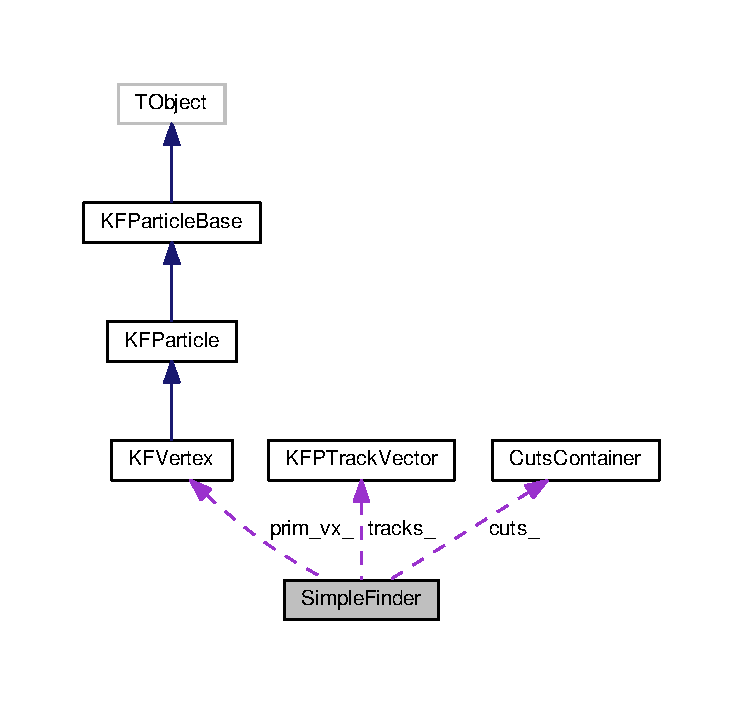
\includegraphics[width=350pt]{classSimpleFinder__coll__graph}
\end{center}
\end{figure}
\subsection*{Public Member Functions}
\begin{DoxyCompactItemize}
\item 
void {\bfseries Init} (const \hyperlink{classKFPTrackVector}{K\+F\+P\+Track\+Vector} \&tracks, const \hyperlink{classKFVertex}{K\+F\+Vertex} \&pv)\hypertarget{classSimpleFinder_ab882be29eaf3e80f7f754b3a8682dc31}{}\label{classSimpleFinder_ab882be29eaf3e80f7f754b3a8682dc31}

\item 
void {\bfseries Sort\+Tracks} ()\hypertarget{classSimpleFinder_aae81d5b2382f10072b91307af30ba4a2}{}\label{classSimpleFinder_aae81d5b2382f10072b91307af30ba4a2}

\item 
void {\bfseries Find\+Particles} ()\hypertarget{classSimpleFinder_a319d1c4da78badd59a538b9839bb2632}{}\label{classSimpleFinder_a319d1c4da78badd59a538b9839bb2632}

\item 
const \hyperlink{classKFPTrackVector}{K\+F\+P\+Track\+Vector} $\ast$ {\bfseries Get\+Tracks} () const \hypertarget{classSimpleFinder_aa1974407925dcb83efad1c68f40fe888}{}\label{classSimpleFinder_aa1974407925dcb83efad1c68f40fe888}

\item 
const std\+::vector$<$ float $>$ \& {\bfseries Get\+Mass} () const \hypertarget{classSimpleFinder_a381a4edacf6f8196a7298846f2f6f0ce}{}\label{classSimpleFinder_a381a4edacf6f8196a7298846f2f6f0ce}

\item 
const std\+::vector$<$ \hyperlink{classOutputContainer}{Output\+Container} $>$ \& {\bfseries Get\+Lambdas} () const \hypertarget{classSimpleFinder_afad8fd09c999b7aea6097fb0797c860b}{}\label{classSimpleFinder_afad8fd09c999b7aea6097fb0797c860b}

\item 
void {\bfseries Set\+Cuts} (const \hyperlink{classCutsContainer}{Cuts\+Container} \&cuts)\hypertarget{classSimpleFinder_a48534300d76d38ae2aa9f1f70dc92d4e}{}\label{classSimpleFinder_a48534300d76d38ae2aa9f1f70dc92d4e}

\item 
const \hyperlink{classCutsContainer}{Cuts\+Container} \& {\bfseries Get\+Cuts} () const \hypertarget{classSimpleFinder_aaedbd2a273aabbe3a45e00613a7d87d8}{}\label{classSimpleFinder_aaedbd2a273aabbe3a45e00613a7d87d8}

\end{DoxyCompactItemize}
\subsection*{Protected Member Functions}
\begin{DoxyCompactItemize}
\item 
float \hyperlink{classSimpleFinder_aba9d34b1412abc495838a6c5c99b997b}{Calculate\+Chi\+To\+Primary\+Vertex} (const \hyperlink{classKFPTrack}{K\+F\+P\+Track} \&track, const int pid) const \hypertarget{classSimpleFinder_aba9d34b1412abc495838a6c5c99b997b}{}\label{classSimpleFinder_aba9d34b1412abc495838a6c5c99b997b}

\begin{DoxyCompactList}\small\item\em Calculates $\chi^2$ of the track to the primary vertex (PV) \end{DoxyCompactList}\item 
void \hyperlink{classSimpleFinder_a6f67c15111fa7a4c19144acef48f7877}{Calculate\+Params\+In\+P\+CA} (const \hyperlink{classKFPTrack}{K\+F\+P\+Track} \&track1, const int pid1, const \hyperlink{classKFPTrack}{K\+F\+P\+Track} \&track2, const int pid2, std\+::array$<$ float, 8 $>$ \&pars1, std\+::array$<$ float, 8 $>$ \&pars2) const \hypertarget{classSimpleFinder_a6f67c15111fa7a4c19144acef48f7877}{}\label{classSimpleFinder_a6f67c15111fa7a4c19144acef48f7877}

\begin{DoxyCompactList}\small\item\em Recalculates daughters tracks\textquotesingle{} parameters in the point of their closest approach. \end{DoxyCompactList}\item 
float \hyperlink{classSimpleFinder_ab2ae6ae5184a0343e9256bf2a57fa3f4}{Calculate\+Distance\+Between\+Particles} (const std\+::array$<$ float, 8 $>$ \&pars1, const std\+::array$<$ float, 8 $>$ \&pars2) const \hypertarget{classSimpleFinder_ab2ae6ae5184a0343e9256bf2a57fa3f4}{}\label{classSimpleFinder_ab2ae6ae5184a0343e9256bf2a57fa3f4}

\begin{DoxyCompactList}\small\item\em Calculates the distance between daughter tracks in their closest approach. \end{DoxyCompactList}\item 
float \hyperlink{classSimpleFinder_adf804cbf61f06440529c38f703182030}{Calculate\+Cos\+Momentum\+Sum} (const std\+::array$<$ float, 8 $>$ \&pars1, const std\+::array$<$ float, 8 $>$ \&pars2) const \hypertarget{classSimpleFinder_adf804cbf61f06440529c38f703182030}{}\label{classSimpleFinder_adf804cbf61f06440529c38f703182030}

\begin{DoxyCompactList}\small\item\em Calculates the cosine of the angle between daughter\textquotesingle{}s and mother\textquotesingle{}s momenta. \end{DoxyCompactList}\item 
\hyperlink{classKFParticleSIMD}{K\+F\+Particle\+S\+I\+MD} \hyperlink{classSimpleFinder_a10ef8ed683c90625963c3185e5399771}{Construct\+Mother} (const \hyperlink{classKFPTrack}{K\+F\+P\+Track} \&track1, const int pid1, const \hyperlink{classKFPTrack}{K\+F\+P\+Track} \&track2, const int pid2) const \hypertarget{classSimpleFinder_a10ef8ed683c90625963c3185e5399771}{}\label{classSimpleFinder_a10ef8ed683c90625963c3185e5399771}

\begin{DoxyCompactList}\small\item\em Creates mother particle as the \hyperlink{classKFParticleSIMD}{K\+F\+Particle\+S\+I\+MD} object. \end{DoxyCompactList}\item 
float \hyperlink{classSimpleFinder_ab174fa409931711f1e2cc650b73922fb}{Calculate\+Chi2\+Geo} (const \hyperlink{classKFParticleSIMD}{K\+F\+Particle\+S\+I\+MD} mother) const \hypertarget{classSimpleFinder_ab174fa409931711f1e2cc650b73922fb}{}\label{classSimpleFinder_ab174fa409931711f1e2cc650b73922fb}

\begin{DoxyCompactList}\small\item\em Calculates $\chi^2$ of daughters\textquotesingle{} tracks in their closest approach. \end{DoxyCompactList}\item 
void \hyperlink{classSimpleFinder_a3cad4e43c94a2a57960ab867eb4207e0}{Calculate\+Mother\+Properties} (const \hyperlink{classKFParticleSIMD}{K\+F\+Particle\+S\+I\+MD} mother, float \&l, float \&ldl, int \&is\+From\+PV) const \hypertarget{classSimpleFinder_a3cad4e43c94a2a57960ab867eb4207e0}{}\label{classSimpleFinder_a3cad4e43c94a2a57960ab867eb4207e0}

\begin{DoxyCompactList}\small\item\em Calculates distance between primary and secondary vertices with error and determines whether mother comes from the PV. \end{DoxyCompactList}\item 
float \hyperlink{classSimpleFinder_a874a6c11539d459f53e86c364c0f2892}{Calculate\+Cos\+Topo} (const \hyperlink{classKFParticleSIMD}{K\+F\+Particle\+S\+I\+MD} mother) const \hypertarget{classSimpleFinder_a874a6c11539d459f53e86c364c0f2892}{}\label{classSimpleFinder_a874a6c11539d459f53e86c364c0f2892}

\begin{DoxyCompactList}\small\item\em Calculates cosine of the angle between reconstructed mother\textquotesingle{}s momentum and mother\textquotesingle{}s radius vector beginning in the PV. \end{DoxyCompactList}\item 
float \hyperlink{classSimpleFinder_a8f5b04879c31465d5ef061f43bc5a74a}{Calculate\+Chi2\+Topo} (const \hyperlink{classKFParticleSIMD}{K\+F\+Particle\+S\+I\+MD} mother) const \hypertarget{classSimpleFinder_a8f5b04879c31465d5ef061f43bc5a74a}{}\label{classSimpleFinder_a8f5b04879c31465d5ef061f43bc5a74a}

\begin{DoxyCompactList}\small\item\em Calculates $\chi^2$ of the mother\textquotesingle{}s track to the PV. \end{DoxyCompactList}\item 
void \hyperlink{classSimpleFinder_af48bcd80810a3c514379ebd68f88f83c}{Save\+Particle} (\hyperlink{classOutputContainer}{Output\+Container} Lambda)\hypertarget{classSimpleFinder_af48bcd80810a3c514379ebd68f88f83c}{}\label{classSimpleFinder_af48bcd80810a3c514379ebd68f88f83c}

\begin{DoxyCompactList}\small\item\em Saves selected particle with set of geometrical decay parameters. \end{DoxyCompactList}\end{DoxyCompactItemize}
\subsection*{Protected Attributes}
\begin{DoxyCompactItemize}
\item 
\hyperlink{classKFPTrackVector}{K\+F\+P\+Track\+Vector} {\bfseries tracks\+\_\+}\hypertarget{classSimpleFinder_a224eaba7c5a7830b730d15ae29e44088}{}\label{classSimpleFinder_a224eaba7c5a7830b730d15ae29e44088}

\item 
\hyperlink{classKFVertex}{K\+F\+Vertex} {\bfseries prim\+\_\+vx\+\_\+}\hypertarget{classSimpleFinder_aac6ae91fb844a0f67ffc31fe4ad09993}{}\label{classSimpleFinder_aac6ae91fb844a0f67ffc31fe4ad09993}

\item 
std\+::array$<$ std\+::vector$<$ int $>$, k\+Number\+Of\+Track\+Types $>$ {\bfseries tr\+Index\+\_\+}\hypertarget{classSimpleFinder_a290194488ca3d915194d9e5cc7169863}{}\label{classSimpleFinder_a290194488ca3d915194d9e5cc7169863}

\item 
\hyperlink{classCutsContainer}{Cuts\+Container} {\bfseries cuts\+\_\+}\hypertarget{classSimpleFinder_a7c2a911d99f8e634e47a68593d57291c}{}\label{classSimpleFinder_a7c2a911d99f8e634e47a68593d57291c}

\item 
float {\bfseries mass\+\_\+}\hypertarget{classSimpleFinder_aaa7bb0079c554838652b89905f1f0684}{}\label{classSimpleFinder_aaa7bb0079c554838652b89905f1f0684}

\item 
std\+::vector$<$ float $>$ {\bfseries vec\+\_\+mass\+\_\+}\hypertarget{classSimpleFinder_a1a259ed53902aefa2616e122114f7ef0}{}\label{classSimpleFinder_a1a259ed53902aefa2616e122114f7ef0}

\item 
std\+::vector$<$ \hyperlink{classOutputContainer}{Output\+Container} $>$ {\bfseries vec\+\_\+lambda\+\_\+}\hypertarget{classSimpleFinder_a80c1c67985d99f3ff0f68b9773fb7aa9}{}\label{classSimpleFinder_a80c1c67985d99f3ff0f68b9773fb7aa9}

\end{DoxyCompactItemize}


The documentation for this class was generated from the following files\+:\begin{DoxyCompactItemize}
\item 
/home/user/cbmdir/kfpf/\+K\+F\+Particle/\+K\+F\+Simple/Simple\+Finder.\+h\item 
/home/user/cbmdir/kfpf/\+K\+F\+Particle/\+K\+F\+Simple/Simple\+Finder.\+cxx\end{DoxyCompactItemize}

%--- End generated contents ---

% Index
\backmatter
\newpage
\phantomsection
\clearemptydoublepage
\addcontentsline{toc}{chapter}{Index}
\printindex

\end{document}
